

 \documentclass[a4paper]{asimbook}

   \usepackage{a4wide}
   \usepackage{makeidx}
   \usepackage{fancyhdr}
   \usepackage{graphicx}
   \usepackage{multicol}
   \usepackage{float}
   \usepackage{textcomp}
   \usepackage{alltt}
   \usepackage{times}
   \ifx\pdfoutput\undefined
     \usepackage[ps2pdf,pagebackref=true,colorlinks=true,linkcolor=blue]{hyperref}
     \usepackage{pspicture}
   \else
     \usepackage[pdftex,pagebackref=true,colorlinks=true,linkcolor=blue]{hyperref}
   \fi
   \usepackage{doxygen}

   \makeindex
   \setcounter{tocdepth}{1}
   \renewcommand{\footrulewidth}{0.4pt}
   \raggedbottom


 \begin{document}

   \begin{titlepage}
     \vspace*{7cm}
     \begin{center}
     {\Large Hurricane Reference Manual\\[1ex]\large 3.\+0 }\\
     \vspace*{1cm}
     {\large Generated by Doxygen 1.8.14}\\
     \vspace*{0.5cm}
     {\small Thu Nov 12 2020 13:58:48}\\
     \end{center}
   \end{titlepage}

   \clearemptydoublepage
   \pagenumbering{roman}

   \tableofcontents
   \clearemptydoublepage

   \pagenumbering{arabic}
\chapter{Hurricane Documentation}
\label{index}\hypertarget{index}{}Additionnal documents\+:
\begin{DoxyItemize}
\item \mbox{\hyperlink{group__grpSynthHierarchy}{Synthetic Class Hierarchy}} 
\end{DoxyItemize}
\chapter{Module Index}
\section{Modules}
Here is a list of all modules\+:\begin{DoxyCompactList}
\item \contentsline{section}{Synthetic Class Hierarchy}{\pageref{group__grpSynthHierarchy}}{}
\item \contentsline{section}{Global Routing Loading}{\pageref{group__LoadGlobalRouting}}{}
\item Generalities{\ttfamily  \mbox{[}external\mbox{]}}\item J\+S\+ON Support{\ttfamily  \mbox{[}external\mbox{]}}\item Db\+U/\+Unit description{\ttfamily  \mbox{[}external\mbox{]}}\item Graphics{\ttfamily  \mbox{[}external\mbox{]}}\end{DoxyCompactList}

\chapter{Namespace Index}
\subsection{Namespace List}
Here is a list of all documented namespaces with brief descriptions\+:\begin{DoxyCompactList}
\item\contentsline{section}{\mbox{\hyperlink{namespaceanonymous__namespace_02AutoSegment_8cpp_03}{anonymous\+\_\+namespace\{\+Auto\+Segment.\+cpp\}}} }{\pageref{namespaceanonymous__namespace_02AutoSegment_8cpp_03}}{}
\item\contentsline{section}{\mbox{\hyperlink{namespaceanonymous__namespace_02ChipTools_8cpp_03}{anonymous\+\_\+namespace\{\+Chip\+Tools.\+cpp\}}} }{\pageref{namespaceanonymous__namespace_02ChipTools_8cpp_03}}{}
\item\contentsline{section}{\mbox{\hyperlink{namespaceanonymous__namespace_02GCell_8cpp_03}{anonymous\+\_\+namespace\{\+G\+Cell.\+cpp\}}} }{\pageref{namespaceanonymous__namespace_02GCell_8cpp_03}}{}
\item\contentsline{section}{\mbox{\hyperlink{namespaceanonymous__namespace_02KatabaticEngine_8cpp_03}{anonymous\+\_\+namespace\{\+Katabatic\+Engine.\+cpp\}}} }{\pageref{namespaceanonymous__namespace_02KatabaticEngine_8cpp_03}}{}
\item\contentsline{section}{\mbox{\hyperlink{namespaceanonymous__namespace_02LoadGrByNet_8cpp_03}{anonymous\+\_\+namespace\{\+Load\+Gr\+By\+Net.\+cpp\}}} }{\pageref{namespaceanonymous__namespace_02LoadGrByNet_8cpp_03}}{}
\item\contentsline{section}{\mbox{\hyperlink{namespaceanonymous__namespace_02Manipulator_8cpp_03}{anonymous\+\_\+namespace\{\+Manipulator.\+cpp\}}} }{\pageref{namespaceanonymous__namespace_02Manipulator_8cpp_03}}{}
\item\contentsline{section}{\mbox{\hyperlink{namespaceanonymous__namespace_02NegociateWindow_8cpp_03}{anonymous\+\_\+namespace\{\+Negociate\+Window.\+cpp\}}} }{\pageref{namespaceanonymous__namespace_02NegociateWindow_8cpp_03}}{}
\item\contentsline{section}{\mbox{\hyperlink{namespaceanonymous__namespace_02RoutingPlane_8cpp_03}{anonymous\+\_\+namespace\{\+Routing\+Plane.\+cpp\}}} }{\pageref{namespaceanonymous__namespace_02RoutingPlane_8cpp_03}}{}
\item\contentsline{section}{\mbox{\hyperlink{namespaceanonymous__namespace_02SegmentFsm_8cpp_03}{anonymous\+\_\+namespace\{\+Segment\+Fsm.\+cpp\}}} }{\pageref{namespaceanonymous__namespace_02SegmentFsm_8cpp_03}}{}
\item\contentsline{section}{\mbox{\hyperlink{namespaceanonymous__namespace_02Session_8cpp_03}{anonymous\+\_\+namespace\{\+Session.\+cpp\}}} }{\pageref{namespaceanonymous__namespace_02Session_8cpp_03}}{}
\item\contentsline{section}{\mbox{\hyperlink{namespaceanonymous__namespace_02Track_8cpp_03}{anonymous\+\_\+namespace\{\+Track.\+cpp\}}} }{\pageref{namespaceanonymous__namespace_02Track_8cpp_03}}{}
\item\contentsline{section}{\mbox{\hyperlink{namespaceanonymous__namespace_02TrackElement_8cpp_03}{anonymous\+\_\+namespace\{\+Track\+Element.\+cpp\}}} }{\pageref{namespaceanonymous__namespace_02TrackElement_8cpp_03}}{}
\item\contentsline{section}{\mbox{\hyperlink{namespaceKite}{Kite}} \\*The namespace dedicated to \mbox{\hyperlink{namespaceKite}{Kite}} }{\pageref{namespaceKite}}{}
\end{DoxyCompactList}

\chapter{Hierarchical Index}
\doxysection{Class Hierarchy}
This inheritance list is sorted roughly, but not completely, alphabetically\+:\begin{DoxyCompactList}
\item \contentsline{section}{Hurricane\+::Box}{\pageref{classHurricane_1_1Box}}{}
\item \contentsline{section}{Hurricane\+::Collection$<$ Type $>$}{\pageref{classHurricane_1_1Collection}}{}
\begin{DoxyCompactList}
\item \contentsline{section}{Hurricane\+::Generic\+Collection$<$ Type $>$}{\pageref{classHurricane_1_1GenericCollection}}{}
\item \contentsline{section}{Hurricane\+::Sub\+Set\+Collection$<$ Type $>$}{\pageref{classHurricane_1_1SubSetCollection}}{}
\end{DoxyCompactList}
\item \contentsline{section}{Hurricane\+::Collection$<$ Cell $\ast$ $>$}{\pageref{classHurricane_1_1Collection}}{}
\item \contentsline{section}{Hurricane\+::Collection$<$ Element $>$}{\pageref{classHurricane_1_1Collection}}{}
\begin{DoxyCompactList}
\item \contentsline{section}{Hurricane\+::Generic\+Collection$<$ Element $>$}{\pageref{classHurricane_1_1GenericCollection}}{}
\item \contentsline{section}{Hurricane\+::List\+Collection$<$ Element $>$}{\pageref{classHurricane_1_1ListCollection}}{}
\item \contentsline{section}{Hurricane\+::Map\+Collection$<$ Key, Element, Compare $>$}{\pageref{classHurricane_1_1MapCollection}}{}
\item \contentsline{section}{Hurricane\+::Set\+Collection$<$ Element, Compare $>$}{\pageref{classHurricane_1_1SetCollection}}{}
\item \contentsline{section}{Hurricane\+::Vector\+Collection$<$ Element $>$}{\pageref{classHurricane_1_1VectorCollection}}{}
\end{DoxyCompactList}
\item \contentsline{section}{Hurricane\+::Collection$<$ Sub\+Type $>$}{\pageref{classHurricane_1_1Collection}}{}
\begin{DoxyCompactList}
\item \contentsline{section}{Hurricane\+::Sub\+Type\+Collection$<$ Type, Sub\+Type $>$}{\pageref{classHurricane_1_1SubTypeCollection}}{}
\end{DoxyCompactList}
\item \contentsline{section}{Compare\+By\+Id}{\pageref{classEntity_1_1CompareById}}{}
\item \contentsline{section}{Hurricane\+::DBo}{\pageref{classHurricane_1_1DBo}}{}
\begin{DoxyCompactList}
\item \contentsline{section}{Hurricane\+::Data\+Base}{\pageref{classHurricane_1_1DataBase}}{}
\item \contentsline{section}{Hurricane\+::Entity}{\pageref{classHurricane_1_1Entity}}{}
\begin{DoxyCompactList}
\item \contentsline{section}{Hurricane\+::Cell}{\pageref{classHurricane_1_1Cell}}{}
\item \contentsline{section}{Hurricane\+::Go}{\pageref{classHurricane_1_1Go}}{}
\begin{DoxyCompactList}
\item \contentsline{section}{Hurricane\+::Component}{\pageref{classHurricane_1_1Component}}{}
\begin{DoxyCompactList}
\item \contentsline{section}{Hurricane\+::Contact}{\pageref{classHurricane_1_1Contact}}{}
\begin{DoxyCompactList}
\item \contentsline{section}{Hurricane\+::Pin}{\pageref{classHurricane_1_1Pin}}{}
\end{DoxyCompactList}
\item \contentsline{section}{Hurricane\+::Diagonal}{\pageref{classHurricane_1_1Diagonal}}{}
\item \contentsline{section}{Hurricane\+::Pad}{\pageref{classHurricane_1_1Pad}}{}
\item \contentsline{section}{Hurricane\+::Plug}{\pageref{classHurricane_1_1Plug}}{}
\item \contentsline{section}{Hurricane\+::Polygon}{\pageref{classHurricane_1_1Polygon}}{}
\item \contentsline{section}{Hurricane\+::Routing\+Pad}{\pageref{classHurricane_1_1RoutingPad}}{}
\item \contentsline{section}{Hurricane\+::Segment}{\pageref{classHurricane_1_1Segment}}{}
\begin{DoxyCompactList}
\item \contentsline{section}{Hurricane\+::Horizontal}{\pageref{classHurricane_1_1Horizontal}}{}
\item \contentsline{section}{Hurricane\+::Vertical}{\pageref{classHurricane_1_1Vertical}}{}
\end{DoxyCompactList}
\end{DoxyCompactList}
\item \contentsline{section}{Hurricane\+::Instance}{\pageref{classHurricane_1_1Instance}}{}
\item \contentsline{section}{Hurricane\+::Rubber}{\pageref{classHurricane_1_1Rubber}}{}
\end{DoxyCompactList}
\item \contentsline{section}{Hurricane\+::Net}{\pageref{classHurricane_1_1Net}}{}
\end{DoxyCompactList}
\item \contentsline{section}{Hurricane\+::Layer}{\pageref{classHurricane_1_1Layer}}{}
\begin{DoxyCompactList}
\item \contentsline{section}{Hurricane\+::Basic\+Layer}{\pageref{classHurricane_1_1BasicLayer}}{}
\item \contentsline{section}{Hurricane\+::Contact\+Layer}{\pageref{classHurricane_1_1ContactLayer}}{}
\item \contentsline{section}{Hurricane\+::Diffusion\+Layer}{\pageref{classHurricane_1_1DiffusionLayer}}{}
\item \contentsline{section}{Hurricane\+::Regular\+Layer}{\pageref{classHurricane_1_1RegularLayer}}{}
\item \contentsline{section}{Hurricane\+::Transistor\+Layer}{\pageref{classHurricane_1_1TransistorLayer}}{}
\item \contentsline{section}{Hurricane\+::Via\+Layer}{\pageref{classHurricane_1_1ViaLayer}}{}
\end{DoxyCompactList}
\item \contentsline{section}{Hurricane\+::Library}{\pageref{classHurricane_1_1Library}}{}
\item \contentsline{section}{Hurricane\+::Quark}{\pageref{classHurricane_1_1Quark}}{}
\item \contentsline{section}{Hurricane\+::Technology}{\pageref{classHurricane_1_1Technology}}{}
\end{DoxyCompactList}
\item \contentsline{section}{Hurricane\+::DbU}{\pageref{classHurricane_1_1DbU}}{}
\item \contentsline{section}{Hurricane\+::Debug\+Session}{\pageref{classHurricane_1_1DebugSession}}{}
\item \contentsline{section}{Hurricane\+::Net\+::Direction}{\pageref{classHurricane_1_1Net_1_1Direction}}{}
\item \contentsline{section}{Hurricane\+::Exception}{\pageref{classHurricane_1_1Exception}}{}
\begin{DoxyCompactList}
\item \contentsline{section}{Hurricane\+::Error}{\pageref{classHurricane_1_1Error}}{}
\item \contentsline{section}{Hurricane\+::Interruption}{\pageref{classHurricane_1_1Interruption}}{}
\item \contentsline{section}{Hurricane\+::Warning}{\pageref{classHurricane_1_1Warning}}{}
\end{DoxyCompactList}
\item \contentsline{section}{Hurricane\+::Filter$<$ Type $>$}{\pageref{classHurricane_1_1Filter}}{}
\begin{DoxyCompactList}
\item \contentsline{section}{Hurricane\+::Generic\+Filter$<$ Type $>$}{\pageref{classHurricane_1_1GenericFilter}}{}
\item \contentsline{section}{Hurricane\+::Not\+Filter$<$ Type $>$}{\pageref{classHurricane_1_1NotFilter}}{}
\end{DoxyCompactList}
\item \contentsline{section}{Hurricane\+::Hook}{\pageref{classHurricane_1_1Hook}}{}
\begin{DoxyCompactList}
\item \contentsline{section}{Hurricane\+::Component\+::Body\+Hook}{\pageref{classHurricane_1_1Component_1_1BodyHook}}{}
\item \contentsline{section}{Hurricane\+::Contact\+::Anchor\+Hook}{\pageref{classHurricane_1_1Contact_1_1AnchorHook}}{}
\item \contentsline{section}{Hurricane\+::Segment\+::Source\+Hook}{\pageref{classHurricane_1_1Segment_1_1SourceHook}}{}
\item \contentsline{section}{Hurricane\+::Segment\+::Target\+Hook}{\pageref{classHurricane_1_1Segment_1_1TargetHook}}{}
\end{DoxyCompactList}
\item \contentsline{section}{Hurricane\+::Hyper\+Net}{\pageref{classHurricane_1_1HyperNet}}{}
\item \contentsline{section}{Hurricane\+::Initializer$<$ T $>$}{\pageref{classHurricane_1_1Initializer}}{}
\item \contentsline{section}{Hurricane\+::Interval}{\pageref{classHurricane_1_1Interval}}{}
\item \contentsline{section}{Hurricane\+::Json\+Object}{\pageref{classHurricane_1_1JsonObject}}{}
\item \contentsline{section}{Hurricane\+::Json\+Stack}{\pageref{classHurricane_1_1JsonStack}}{}
\item \contentsline{section}{Hurricane\+::Locator$<$ Type $>$}{\pageref{classHurricane_1_1Locator}}{}
\begin{DoxyCompactList}
\item \contentsline{section}{Hurricane\+::Generic\+Locator$<$ Type $>$}{\pageref{classHurricane_1_1GenericLocator}}{}
\end{DoxyCompactList}
\item \contentsline{section}{Hurricane\+::Locator$<$ Cell $\ast$ $>$}{\pageref{classHurricane_1_1Locator}}{}
\item \contentsline{section}{Hurricane\+::Locator$<$ Element $>$}{\pageref{classHurricane_1_1Locator}}{}
\begin{DoxyCompactList}
\item \contentsline{section}{Hurricane\+::Generic\+Locator$<$ Element $>$}{\pageref{classHurricane_1_1GenericLocator}}{}
\end{DoxyCompactList}
\item \contentsline{section}{Hurricane\+::Locator$<$ El\+Type $>$}{\pageref{classHurricane_1_1Locator}}{}
\item \contentsline{section}{Hurricane\+::Locator$<$ Hurricane\+::DBo $\ast$ $>$}{\pageref{classHurricane_1_1Locator}}{}
\item \contentsline{section}{Hurricane\+::Locator$<$ Hurricane\+::Instance $\ast$ $>$}{\pageref{classHurricane_1_1Locator}}{}
\item \contentsline{section}{Hurricane\+::Locator$<$ Sub\+Type $>$}{\pageref{classHurricane_1_1Locator}}{}
\item \contentsline{section}{Hurricane\+::Basic\+Layer\+::Material}{\pageref{classHurricane_1_1BasicLayer_1_1Material}}{}
\item \contentsline{section}{Hurricane\+::Name}{\pageref{classHurricane_1_1Name}}{}
\item \contentsline{section}{Hurricane\+::Occurrence}{\pageref{classHurricane_1_1Occurrence}}{}
\item \contentsline{section}{Hurricane\+::Transformation\+::Orientation}{\pageref{classHurricane_1_1Transformation_1_1Orientation}}{}
\item \contentsline{section}{Hurricane\+::Path}{\pageref{classHurricane_1_1Path}}{}
\item \contentsline{section}{Hurricane\+::Physical\+Rule}{\pageref{classHurricane_1_1PhysicalRule}}{}
\item \contentsline{section}{Hurricane\+::Instance\+::Placement\+Status}{\pageref{classHurricane_1_1Instance_1_1PlacementStatus}}{}
\item \contentsline{section}{Hurricane\+::Point}{\pageref{classHurricane_1_1Point}}{}
\item \contentsline{section}{Hurricane\+::Property}{\pageref{classHurricane_1_1Property}}{}
\begin{DoxyCompactList}
\item \contentsline{section}{Hurricane\+::Private\+Property}{\pageref{classHurricane_1_1PrivateProperty}}{}
\begin{DoxyCompactList}
\item \contentsline{section}{Hurricane\+::Standard\+Private\+Property$<$ Value, Json\+State $>$}{\pageref{classHurricane_1_1StandardPrivateProperty}}{}
\item \contentsline{section}{Isobar\+::Py\+Holder\+Property}{\pageref{classIsobar_1_1PyHolderProperty}}{}
\end{DoxyCompactList}
\item \contentsline{section}{Hurricane\+::Shared\+Property}{\pageref{classHurricane_1_1SharedProperty}}{}
\begin{DoxyCompactList}
\item \contentsline{section}{Hurricane\+::Relation}{\pageref{classHurricane_1_1Relation}}{}
\begin{DoxyCompactList}
\item \contentsline{section}{Hurricane\+::Standard\+Relation}{\pageref{classHurricane_1_1StandardRelation}}{}
\end{DoxyCompactList}
\item \contentsline{section}{Hurricane\+::Standard\+Shared\+Property$<$ Value $>$}{\pageref{classHurricane_1_1StandardSharedProperty}}{}
\item \contentsline{section}{Hurricane\+::Update\+Session}{\pageref{classHurricane_1_1UpdateSession}}{}
\end{DoxyCompactList}
\end{DoxyCompactList}
\item \contentsline{section}{Isobar\+::Py\+Attributes\+Holder}{\pageref{structIsobar_1_1PyAttributesHolder}}{}
\item \contentsline{section}{Isobar\+::Python\+Attributes}{\pageref{classIsobar_1_1PythonAttributes}}{}
\item \contentsline{section}{Hurricane\+::Quad\+Tree}{\pageref{classHurricane_1_1QuadTree}}{}
\item \contentsline{section}{Hurricane\+::Query}{\pageref{classHurricane_1_1Query}}{}
\item \contentsline{section}{Hurricane\+::Slice}{\pageref{classHurricane_1_1Slice}}{}
\item \contentsline{section}{Hurricane\+::Tabulation}{\pageref{classHurricane_1_1Tabulation}}{}
\item \contentsline{section}{Hurricane\+::Transformation}{\pageref{classHurricane_1_1Transformation}}{}
\item \contentsline{section}{tstream}{\pageref{clasststream}}{}
\item \contentsline{section}{Hurricane\+::Net\+::Type}{\pageref{classHurricane_1_1Net_1_1Type}}{}
\end{DoxyCompactList}

\chapter{Class Index}
\doxysection{Class List}
Here are the classes, structs, unions and interfaces with brief descriptions\+:\begin{DoxyCompactList}
\item\contentsline{section}{\mbox{\hyperlink{classpython_1_1capacitormatrix_1_1CapacitorStack}{Capacitor\+Stack}} \\*Draws the layout of a compact capacitor or a matrix of adjacent identical capacitors }{\pageref{classpython_1_1capacitormatrix_1_1CapacitorStack}}{}
\item\contentsline{section}{\mbox{\hyperlink{classpython_1_1capacitorunit_1_1CapacitorUnit}{Capacitor\+Unit}} \\*Draws a capacitor of type Poly-\/\+Poly or Metal-\/\+Metal in 350 nm AMS CMOS technology }{\pageref{classpython_1_1capacitorunit_1_1CapacitorUnit}}{}
\item\contentsline{section}{\mbox{\hyperlink{classpython_1_1capacitorrouted_1_1RoutMatchedCapacitor}{Rout\+Matched\+Capacitor}} \\*Routs two matched capacitors, C1 and C2, drawn in a capacitor matrix }{\pageref{classpython_1_1capacitorrouted_1_1RoutMatchedCapacitor}}{}
\item\contentsline{section}{\mbox{\hyperlink{classpython_1_1stack_1_1Stack}{Stack}} \\*Draw a \mbox{\hyperlink{classpython_1_1stack_1_1Stack}{Stack}} of Transistors }{\pageref{classpython_1_1stack_1_1Stack}}{}
\item\contentsline{section}{\mbox{\hyperlink{classpython_1_1capacitorvrtracks_1_1VerticalRoutingTracks}{Vertical\+Routing\+Tracks}} \\*Route two matched capacitors, C1 and C2, drawn in a capacitor matrix }{\pageref{classpython_1_1capacitorvrtracks_1_1VerticalRoutingTracks}}{}
\end{DoxyCompactList}

\chapter{Module Documentation}
\hypertarget{group__Generalities}{}\doxysection{Generalities}
\label{group__Generalities}\index{Generalities@{Generalities}}


The supporting paraphernalia.  


The supporting paraphernalia. 

\hypertarget{group__Generalities_secGeneralitiesIntro}{}\doxysubsection{Introduction}\label{group__Generalities_secGeneralitiesIntro}
When documenting a given class, only member functions introducted by this class are documented, inherited ones are not repeated. This is made easier by the presence of the inheritance sub-\/tree containing the described object type.

In the same way, some opetators or global functions are defined for all object types though they don\textquotesingle{}t derive from a common base class. Those operators and generic functions will be described below.

terminology In the following, we will describe operators and functions applying to objects of different types. Therefore we will name \char`\"{}\+Object\char`\"{} any of those types.\hypertarget{group__Generalities_secGeneralitiesNammingConventions}{}\doxysubsection{Namming conventions}\label{group__Generalities_secGeneralitiesNammingConventions}
The name of \char`\"{}\+C macros\char`\"{} are written with lower case letters and underscores (examples \+: {\bfseries{is\+\_\+a}}, {\bfseries{for\+\_\+each\+\_\+cell}} or {\bfseries{end\+\_\+for}}) while the name of generic functions and member functions never use the underscore and always start with an Upper case letter (examples \+: {\bfseries{Get\+Unit}}, {\bfseries{Get\+Master\+Cell}}, {\bfseries{Is\+Called\+By}}).

\begin{DoxyRemark}{Remarks}
When examining {\ttfamily }.h include files for more detailed information you will find member functions which start with an underscore. {\bfseries{While being \char`\"{}public\char`\"{} those functions must never be called upon}}. In principle, only here\textquotesingle{}after documented functions should be used by the application programmer.
\end{DoxyRemark}
\hypertarget{group__Generalities_secGeneralitiesGetString}{}\doxysubsection{Get\+String}\label{group__Generalities_secGeneralitiesGetString}

\begin{DoxyCode}{0}
\DoxyCodeLine{\textcolor{keywordtype}{string} GetString(\textcolor{keyword}{const} Object\& \textcolor{keywordtype}{object});}
\DoxyCodeLine{\textcolor{keywordtype}{string} GetString(\textcolor{keyword}{const} Object* \textcolor{keywordtype}{object});}

\end{DoxyCode}
 Thoses generic function allows you to get into a string an explicit description of any kind of \mbox{\hyperlink{namespaceHurricane}{Hurricane}} object pointer or reference. 
\begin{DoxyCode}{0}
\DoxyCodeLine{ostream\& operator<< (ostream\& stream, \textcolor{keyword}{const} Object\& \textcolor{keywordtype}{object});}
\DoxyCodeLine{ostream\& operator<< (ostream\& stream, \textcolor{keyword}{const} Object* \textcolor{keywordtype}{object});}

\end{DoxyCode}
 All \mbox{\hyperlink{namespaceHurricane}{Hurricane}} objects have printing operators for a reference or a pointer. Those printing operators use the generic function Hurricane\+::\+Get\+String() previously studied.\hypertarget{group__Generalities_secGeneralitiesPredicates}{}\doxysubsection{Predicates}\label{group__Generalities_secGeneralitiesPredicates}
The {\ttfamily bool} {\ttfamily is\+\_\+a$<$\+Type$\ast$$>$(object)} function.

For any kind of \mbox{\hyperlink{namespaceHurricane}{Hurricane}} object pertaining to a class with at least one \char`\"{}virtual\char`\"{} member, it is possible to determine if this object is a type or a sub-\/type of {\ttfamily $<$type$>$} as shown in the following example\+: 
\begin{DoxyCode}{0}
\DoxyCodeLine{DataBase* dataBase = GetDataBase();}
\DoxyCodeLine{ }
\DoxyCodeLine{Library* library = Library::Create(dataBase, \textcolor{stringliteral}{"{}std"{}});}
\DoxyCodeLine{ }
\DoxyCodeLine{Cell* cell = Cell::Create(library, \textcolor{stringliteral}{"{}nand"{}});}
\DoxyCodeLine{ }
\DoxyCodeLine{\textcolor{keywordflow}{if} (is\_a<Cell*>(cell)) \{}
\DoxyCodeLine{   \textcolor{comment}{// will inevitably go through here}}
\DoxyCodeLine{\}}
\DoxyCodeLine{ }
\DoxyCodeLine{\textcolor{keywordflow}{if} (is\_a<Entity*>(cell)) \{}
\DoxyCodeLine{   \textcolor{comment}{// will go through here also because Cell derives from Entity}}
\DoxyCodeLine{\}}
\DoxyCodeLine{ }
\DoxyCodeLine{\textcolor{keywordflow}{if} (is\_a<Library*>(cell)) \{}
\DoxyCodeLine{   \textcolor{comment}{// will never go through here because Cell doesn't derive from Library}}
\DoxyCodeLine{\}}

\end{DoxyCode}
\hypertarget{group__Generalities_secGeneralitiesInheritance}{}\doxysubsection{Inheritance}\label{group__Generalities_secGeneralitiesInheritance}
All classes deriving directly from a base class define a new type named {\bfseries{Inherit}} which represents this base class. {\bfseries{This one is unique because \mbox{\hyperlink{namespaceHurricane}{Hurricane}} doesn\textquotesingle{}t use multiple inheritance}}. This type is important because it allows to call upon the methods of the base class without knowing its name as shown in the following example\+: 
\begin{DoxyCode}{0}
\DoxyCodeLine{\textcolor{keywordtype}{void} MyObject::Draw() const}
\DoxyCodeLine{\textcolor{comment}{// ************************}}
\DoxyCodeLine{\{}
\DoxyCodeLine{   Inherit::Draw();}
\DoxyCodeLine{ }
\DoxyCodeLine{   DrawParticularities();}
\DoxyCodeLine{\}}

\end{DoxyCode}
\hypertarget{group__Generalities_secGeneralitiesTraceUtilities}{}\doxysubsection{Trace utilities}\label{group__Generalities_secGeneralitiesTraceUtilities}
The library provides some usefull utilities for generating trace printings with a natural indentation allowing better understanding of the processing sequences\+:


\begin{DoxyItemize}
\item {\bfseries{Hurricane\+::in\+\_\+trace}} 
\item {\bfseries{Hurricane\+::trace\+\_\+on}} 
\item {\bfseries{Hurricane\+::trace\+\_\+off}} 
\item {\bfseries{Hurricane\+::trace\+\_\+in}} 
\item {\bfseries{Hurricane\+::trace\+\_\+out}} 
\item {\bfseries{Hurricane\+::trace}} 
\end{DoxyItemize}


\begin{DoxyCode}{0}
\DoxyCodeLine{\textcolor{keywordtype}{void} MyFunction(MyData* data)}
\DoxyCodeLine{\textcolor{comment}{// **************************}}
\DoxyCodeLine{\{}
\DoxyCodeLine{   trace << \textcolor{stringliteral}{"{}entering in MyFunction with "{}} << data << endl;}
\DoxyCodeLine{   trace\_in();}
\DoxyCodeLine{ }
\DoxyCodeLine{   ...}
\DoxyCodeLine{ }
\DoxyCodeLine{   trace << \textcolor{stringliteral}{"{}exiting of MyFunction"{}} << endl;}
\DoxyCodeLine{   trace\_out();}
\DoxyCodeLine{\}}

\end{DoxyCode}
 \begin{DoxyRemark}{Remarks}
Debugger enthousiastic users will probably ignore this trace capability which presents the annoying need to be inserted into the code... For myself, I do prefer those facilities...
\end{DoxyRemark}
\hypertarget{group__Generalities_secGeneralitiesRemarks}{}\doxysubsection{Remarks}\label{group__Generalities_secGeneralitiesRemarks}
Many other global and generic functions exist. Each one will be studied within the description of the classes which create or specialize them (example\+: {\bfseries{Hurricane\+::\+Get\+Unit}} will be introduced with the Unit class and {\bfseries{Hurricane\+::\+Get\+Collection}} with the \mbox{\hyperlink{classHurricane_1_1Collection}{Collection}} class). 
\hypertarget{group__JsonSupport}{}\doxysection{JSON Support}
\label{group__JsonSupport}\index{JSON Support@{JSON Support}}


JSON Import/\+Export of the \mbox{\hyperlink{classHurricane_1_1DataBase}{Data\+Base}}.  


\doxysubsection*{Classes}
\begin{DoxyCompactItemize}
\item 
class \mbox{\hyperlink{classHurricane_1_1JsonObject}{Hurricane\+::\+Json\+Object}}
\begin{DoxyCompactList}\small\item\em Support for JSON export. \end{DoxyCompactList}\item 
class \mbox{\hyperlink{classHurricane_1_1JsonStack}{Hurricane\+::\+Json\+Stack}}
\begin{DoxyCompactList}\small\item\em JSON Parser Stack. \end{DoxyCompactList}\end{DoxyCompactItemize}


\doxysubsection{Detailed Description}
JSON Import/\+Export of the \mbox{\hyperlink{classHurricane_1_1DataBase}{Data\+Base}}. 

\hypertarget{group__JsonSupport_secJsonSupportIntro}{}\doxysubsection{Introduction}\label{group__JsonSupport_secJsonSupportIntro}
One key feature of the \mbox{\hyperlink{namespaceHurricane}{Hurricane}} \mbox{\hyperlink{classHurricane_1_1DataBase}{Data\+Base}} is it\textquotesingle{}s hierarchical managment. But unfortunatly the simple approach of saving a design \mbox{\hyperlink{classHurricane_1_1Cell}{Cell}} by \mbox{\hyperlink{classHurricane_1_1Cell}{Cell}}, hierarchical level by hierarchical level makes it very difficult to save the trans-\/hierarchical informations (mainly is the occurrences)

One solution is to save the design and all it\textquotesingle{}s levels, down and including the standard cells. With all the levels saved, we then can add the occurrences and all the attached trans-\/hierarchical informations. We call that comprehensive saving of a design, a {\itshape design blob}.

Instead of creating one more ad-\/hoc format, we just dump the \mbox{\hyperlink{classHurricane_1_1DataBase}{Data\+Base}} objects in a mirror like way in JSON format.

As it is a textual format, the generated files are larges. So the files are compressed through {\ttfamily gzip}.\hypertarget{group__JsonSupport_secJsonSemantic}{}\doxysubsection{JSON Additional Semantic}\label{group__JsonSupport_secJsonSemantic}
To ease the work of the parser, some semantic has been added to the JSON objects representing a \mbox{\hyperlink{namespaceHurricane}{Hurricane}} \mbox{\hyperlink{classHurricane_1_1DataBase}{Data\+Base}}.
\begin{DoxyEnumerate}
\item The first key/value pair must have the key {\ttfamily \char`\"{}@typename\char`\"{}} and give the kind of \mbox{\hyperlink{classHurricane_1_1JsonObject}{Json\+Object}} associated. The value is the string returned by {\ttfamily \mbox{\hyperlink{classHurricane_1_1JsonObject_a947e1c3f8dbae63bb2d086b5b827a2a5}{Json\+Object\+::get\+Type\+Name()}}}.
\item Attributes keys must start by a {\ttfamily \textquotesingle{}\+\_\+\textquotesingle{}} character. (yes, I know, the C++ convention has changed and it should be put at the end).
\item Collections or containers must be put {\itshape after} all the scalar attributes and their keys must start by a {\ttfamily \textquotesingle{}+\textquotesingle{}} character.
\end{DoxyEnumerate}


\begin{DoxyCode}{0}
\DoxyCodeLine{\{}
\DoxyCodeLine{  "{}@typename"{}: "{}Cell"{},}
\DoxyCodeLine{  "{}\_id"{}: 3,}
\DoxyCodeLine{  "{}\_library"{}: "{}RootLibrary.AllianceFramework.sxlib"{},}
\DoxyCodeLine{  "{}\_name"{}: "{}o3\_x2"{},}
\DoxyCodeLine{  "{}\_abutmentBox"{}: \{}
\DoxyCodeLine{    "{}@typename"{}: "{}Box"{},}
\DoxyCodeLine{    "{}\_xMin"{}: 0,}
\DoxyCodeLine{    "{}\_yMin"{}: 0,}
\DoxyCodeLine{    "{}\_xMax"{}: 72000,}
\DoxyCodeLine{    "{}\_yMax"{}: 120000}
\DoxyCodeLine{  \},}
\DoxyCodeLine{  "{}+instanceMap"{}: [],}
\DoxyCodeLine{  "{}+netMap"{}: [}
\DoxyCodeLine{  ],}
\DoxyCodeLine{\}}

\end{DoxyCode}
\hypertarget{group__JsonSupport_secJsonDriver}{}\doxysubsection{JSON Driver Support}\label{group__JsonSupport_secJsonDriver}
The driver is implemented through overloads (template and non-\/template) of the {\ttfamily json\+Writer()} function. For the template overload to work, even for non-\/\+Hurricane classes, it is defined outside the \mbox{\hyperlink{namespaceHurricane}{Hurricane}} namespace.

For POD types, four overloads of {\ttfamily json\+Writer()} are defined\+:


\begin{DoxyCode}{0}
\DoxyCodeLine{\textcolor{keywordtype}{void}  jsonWrite ( JsonWriter* w, \textcolor{keyword}{const} \textcolor{keywordtype}{int}* v );}
\DoxyCodeLine{\textcolor{keywordtype}{void}  jsonWrite ( JsonWriter* w,       \textcolor{keywordtype}{int}  v );}
\DoxyCodeLine{\textcolor{keywordtype}{void}  jsonWrite ( JsonWriter* w, \textcolor{keyword}{const} std::string\& key, \textcolor{keyword}{const} \textcolor{keywordtype}{int}* value )}
\DoxyCodeLine{\textcolor{keywordtype}{void}  jsonWrite ( JsonWriter* w, \textcolor{keyword}{const} std::string\& key,       \textcolor{keywordtype}{int}  value )}

\end{DoxyCode}


The first two writes the object (here\+: {\ttfamily int}) \char`\"{}as is\char`\"{} while the two later writes a pair key/object.

For other class/object that needs to be writen in the JSON file, they must provide a {\ttfamily to\+Json()} function. It doesn\textquotesingle{}t even need to be virtual. For \mbox{\hyperlink{classHurricane_1_1Point}{Point}}\+:


\begin{DoxyCode}{0}
\DoxyCodeLine{\textcolor{keywordtype}{void}  Point::toJson ( JsonWriter* w )\textcolor{keyword}{ const}}
\DoxyCodeLine{\textcolor{keyword}{}\{}
\DoxyCodeLine{  w-\/>startObject();}
\DoxyCodeLine{  jsonWrite( w, \textcolor{stringliteral}{"{}@typename"{}}, \textcolor{stringliteral}{"{}Point"{}} );}
\DoxyCodeLine{  jsonWrite( w, \textcolor{stringliteral}{"{}\_x"{}}, getX() );}
\DoxyCodeLine{  jsonWrite( w, \textcolor{stringliteral}{"{}\_y"{}}, getY() );}
\DoxyCodeLine{  w-\/>endObject();}
\DoxyCodeLine{\}}

\end{DoxyCode}


This function allows three templates of {\ttfamily json\+Write()} to be used with an object of class \mbox{\hyperlink{classHurricane_1_1Point}{Point}}\+:


\begin{DoxyCode}{0}
\DoxyCodeLine{\textcolor{keyword}{template}<\textcolor{keyword}{typename} C>}
\DoxyCodeLine{\textcolor{keywordtype}{void}  jsonWrite ( JsonWriter* w, \textcolor{keyword}{const} C* \textcolor{keywordtype}{object} );}
\DoxyCodeLine{}
\DoxyCodeLine{\textcolor{keyword}{template}<\textcolor{keyword}{typename} C>}
\DoxyCodeLine{\textcolor{keywordtype}{void}  jsonWrite ( JsonWriter* w, \textcolor{keyword}{const} std::string\& key, C* \textcolor{keywordtype}{object} );}
\DoxyCodeLine{}
\DoxyCodeLine{\textcolor{keyword}{template}<\textcolor{keyword}{typename} C>}
\DoxyCodeLine{\textcolor{keywordtype}{void}  jsonWrite ( JsonWriter* w, \textcolor{keyword}{const} std::string\& key, \textcolor{keyword}{const} C* \textcolor{keywordtype}{object} );}

\end{DoxyCode}


Note that through those three overloads we only provides support for pointers to object. The driving mechanism is designed in such a way that passing arguments by value is not supported for non-\/\+POD types. Trying to do so will result in an unsupported message inside the generated JSON file.\hypertarget{group__JsonSupport_secJsonDriverDBo}{}\doxysubsubsection{DBos Special Case}\label{group__JsonSupport_secJsonDriverDBo}
For \mbox{\hyperlink{classHurricane_1_1DBo}{DBo}} objects, a complete parallel hierarchy of Json\+Objects mimicking the one of DBos has been implemented. The {\ttfamily to\+Json()} function is implemented in the \mbox{\hyperlink{classHurricane_1_1DBo}{DBo}} base object, and the derived classes must implement the following virtual functions\+:


\begin{DoxyCode}{0}
\DoxyCodeLine{\textcolor{keyword}{class }DBo \{}
\DoxyCodeLine{  \textcolor{keyword}{public}:}
\DoxyCodeLine{    \textcolor{keyword}{virtual} \textcolor{keywordtype}{void}  \_toJson            ( JsonWriter* ) \textcolor{keyword}{const};}
\DoxyCodeLine{    \textcolor{keyword}{virtual} \textcolor{keywordtype}{void}  \_toJsonCollections ( JsonWriter* ) \textcolor{keyword}{const};}
\DoxyCodeLine{    \textcolor{keyword}{virtual} \textcolor{keywordtype}{void}  \_toJsonSignature   ( JsonWriter* ) \textcolor{keyword}{const};}
\DoxyCodeLine{            \textcolor{keywordtype}{void}  toJson             ( JsonWriter* ) \textcolor{keyword}{const};}
\DoxyCodeLine{            \textcolor{keywordtype}{void}  toJsonSignature    ( JsonWriter* ) \textcolor{keyword}{const};}

\end{DoxyCode}


The JSON driver functions is splitted in two parts\+:
\begin{DoxyItemize}
\item {\ttfamily \+\_\+to\+Json()} must drive the scalar attributes.
\item {\ttfamily \+\_\+to\+Json\+Collections()} must drive the various collections or containers. This is to ensure that all the scalars attributes are put before the collections, event through inheritance.
\end{DoxyItemize}

The additionnal {\ttfamily to\+Json\+Signature()} method provide the signature for an \mbox{\hyperlink{classHurricane_1_1Entity}{Entity}} which is used by an occurrence. The signature of an occurrence is needed when we create a JSON for a \mbox{\hyperlink{classHurricane_1_1Cell}{Cell}} only. In that case we cannot directly save the transhierarchical informations, so we need a way to characterize the deep \mbox{\hyperlink{classHurricane_1_1Entity}{Entity}} (which is not part of the saved \mbox{\hyperlink{classHurricane_1_1Cell}{Cell}}). Most of the time, the signature is the scalar attributes of the occurrenced object, it is far from foolproof, but it will do for now.\hypertarget{group__JsonSupport_secJsonParser}{}\doxysubsection{JSON Parser Support}\label{group__JsonSupport_secJsonParser}
To enable JSON parsing support for an object, say \mbox{\hyperlink{classHurricane_1_1Point}{Point}}, an associated {\ttfamily Json\+Point} class must be created. This class must be derived (directly or not) from \mbox{\hyperlink{classHurricane_1_1JsonObject}{Json\+Object}}. It must implement one static functions and four methods, as shown below.


\begin{DoxyCode}{0}
\DoxyCodeLine{\textcolor{keyword}{class }JsonPoint : \textcolor{keyword}{public} JsonObject \{}
\DoxyCodeLine{  \textcolor{keyword}{public}:}
\DoxyCodeLine{    \textcolor{keyword}{static}  \textcolor{keywordtype}{void}       initialize ();}
\DoxyCodeLine{                       JsonPoint  (\textcolor{keywordtype}{unsigned} \textcolor{keywordtype}{long} flags);}
\DoxyCodeLine{    \textcolor{keyword}{virtual} \textcolor{keywordtype}{string}     getTypeName() \textcolor{keyword}{const};}
\DoxyCodeLine{    \textcolor{keyword}{virtual} JsonPoint* clone      (\textcolor{keywordtype}{unsigned} \textcolor{keywordtype}{long} flags) \textcolor{keyword}{const};}
\DoxyCodeLine{    \textcolor{keyword}{virtual} \textcolor{keywordtype}{void}       toData     (JsonStack\&);}
\DoxyCodeLine{\};}

\end{DoxyCode}


The {\ttfamily initialize()} static function must be present in concrete class only. It is used to register the Json object into the parser during the static initialization of the program.


\begin{DoxyCode}{0}
\DoxyCodeLine{\textcolor{preprocessor}{\#include "{}hurricane/Initializer.h"{}}}
\DoxyCodeLine{\textcolor{preprocessor}{\#include "{}hurricane/Point.h"{}}}
\DoxyCodeLine{}
\DoxyCodeLine{Initializer<JsonPoint>  jsonPointInit ( 0 );}
\DoxyCodeLine{}
\DoxyCodeLine{\textcolor{keywordtype}{void}  JsonPoint::initialize ()}
\DoxyCodeLine{\{ JsonTypes::registerType( \textcolor{keyword}{new} JsonPoint (JsonWriter::RegisterMode) ); \}}

\end{DoxyCode}


The constructor has to declare requirements, attributes, and collections needed to build the \mbox{\hyperlink{classHurricane_1_1DataBase}{Data\+Base}} object. Note the the requirements are not part of the objects but only needed to build it.


\begin{DoxyCode}{0}
\DoxyCodeLine{JsonPoint::JsonPoint ( \textcolor{keywordtype}{unsigned} \textcolor{keywordtype}{long} flags )}
\DoxyCodeLine{  : JsonObject(flags)}
\DoxyCodeLine{\{}
\DoxyCodeLine{  add( \textcolor{stringliteral}{"{}\_x"{}}, \textcolor{keyword}{typeid}(int64\_t) );}
\DoxyCodeLine{  add( \textcolor{stringliteral}{"{}\_y"{}}, \textcolor{keyword}{typeid}(int64\_t) );}
\DoxyCodeLine{\}}

\end{DoxyCode}


The {\ttfamily get\+Type\+Name()} virtual function must return the typename used for the {\ttfamily \char`\"{}@typename\char`\"{}} key in the JSON file. Most of the time it\textquotesingle{}s the same name as the object itself, but not always.


\begin{DoxyCode}{0}
\DoxyCodeLine{\textcolor{keywordtype}{string} JsonPoint::getTypeName ()\textcolor{keyword}{ const}}
\DoxyCodeLine{\textcolor{keyword}{}\{ \textcolor{keywordflow}{return} \textcolor{stringliteral}{"{}Point"{}}; \}}

\end{DoxyCode}


The {\ttfamily clone()} virtual function must return a brand new Json object of the same type. The datas of the orignal object {\bfseries{must}} not be copied. The cloning is about the class type, not the contents.


\begin{DoxyCode}{0}
\DoxyCodeLine{JsonPoint* JsonPoint::clone ( \textcolor{keywordtype}{unsigned} \textcolor{keywordtype}{long} flags )\textcolor{keyword}{ const}}
\DoxyCodeLine{\textcolor{keyword}{}\{ \textcolor{keywordflow}{return} \textcolor{keyword}{new} JsonPoint ( flags ); \}}

\end{DoxyCode}


The {\ttfamily to\+Data()} virtual function actually gather the attributes to recreate the \mbox{\hyperlink{classHurricane_1_1DataBase}{Data\+Base}} object. It needs the parser stack to pull the attributes and to push the created object.


\begin{DoxyCode}{0}
\DoxyCodeLine{\textcolor{keywordtype}{void} JsonPoint::toData ( JsonStack\& stack )}
\DoxyCodeLine{\{}
\DoxyCodeLine{  check( stack, \textcolor{stringliteral}{"{}JsonPoint::toData"{}} );}
\DoxyCodeLine{  Point point ( \mbox{\hyperlink{classHurricane_1_1DbU_aec69d65ec1651c2feea24c5931f4580b}{DbU::fromDb}}(get<int64\_t>(stack,\textcolor{stringliteral}{"{}\_x"{}}))}
\DoxyCodeLine{              , \mbox{\hyperlink{classHurricane_1_1DbU_aec69d65ec1651c2feea24c5931f4580b}{DbU::fromDb}}(get<int64\_t>(stack,\textcolor{stringliteral}{"{}\_y"{}})) );}
\DoxyCodeLine{  update( stack, point );}
\DoxyCodeLine{\}}

\end{DoxyCode}
\hypertarget{group__JsonSupport_secJsonArray}{}\doxysubsubsection{JSON Array}\label{group__JsonSupport_secJsonArray}
JSON array are not translated into containers of any kind. They are simply ignored (from the stack point of view). Objects in array comes from a great variety of containers including \mbox{\hyperlink{classHurricane_1_1Collection}{Hurricane\+::\+Collection}}, in almost all cases, their very constructors are responsibles for inserting the object in the relevant container/collection. So there is no need to build a mechanism to keep track of all the objects in an array through a temporary container.

The corollary is that an object in an array must be able to extract the relevant context information from the stack. Say, if we are in an array of components, they must belong to a \mbox{\hyperlink{classHurricane_1_1Net}{Net}}, which must be present in the stack with a key \char`\"{}.\+Net\char`\"{}.\hypertarget{group__JsonSupport_secJsonStack}{}\doxysubsubsection{Parser Stack}\label{group__JsonSupport_secJsonStack}
While performing the parsing, the parser maintain a stack (\mbox{\hyperlink{classHurricane_1_1JsonStack}{Json\+Stack}}) containing\+:
\begin{DoxyItemize}
\item The stack of attributes translateds, but not consumeds by the parser and the objects currently openeds (that is, which parsing is not completed). This stack contains POD or \mbox{\hyperlink{namespaceHurricane}{Hurricane}} objects (value or pointer). It is a vector of pair {\ttfamily }(key,value) where the {\itshape key} is either the attribute name ({\ttfamily \+\_\+bounding\+Box}, {\ttfamily \+\_\+x\+Min}, {\ttfamily \+\_\+master\+Cell}, ...) or the class name ({\ttfamily }.\mbox{\hyperlink{classHurricane_1_1Net}{Net}}, {\ttfamily }.\mbox{\hyperlink{classHurricane_1_1Cell}{Cell}}, ...).
\item The stack of JSON objects currently openeds, thoses objects are all derived classes of \mbox{\hyperlink{classHurricane_1_1JsonObject}{Json\+Object}}.
\item A stack of currently opened DBo$\ast$. This stack is somewhat redundant with the first, but is needed because {\ttfamily boost\+::any\+\_\+cast$<$$>$} is not able to perform dynamic conversions. You have to know the exact for the conversion to work. Here, everything is DBo$\ast$, so the problem do not arises.
\end{DoxyItemize}\hypertarget{group__JsonSupport_secJsonCycle}{}\doxysubsubsection{Json\+Object Life Cycle}\label{group__JsonSupport_secJsonCycle}

\begin{DoxyCode}{0}
\DoxyCodeLine{\{                          \# JsonDummy()  (1).}
\DoxyCodeLine{  "{}\_typename"{}: "{}Net"{},      \# JsonNet()  CTOR (2).}
\DoxyCodeLine{  "{}\_id"{}: 14622,}
\DoxyCodeLine{  "{}\_name"{}: "{}saccu(0)"{},}
\DoxyCodeLine{  "{}\_isGlobal"{}: false,}
\DoxyCodeLine{  "{}\_isExternal"{}: false,}
\DoxyCodeLine{  "{}\_isAutomatic"{}: false,}
\DoxyCodeLine{  "{}\_type"{}: "{}LOGICAL"{},}
\DoxyCodeLine{  "{}\_direction"{}: "{}-\/-\/-\/-\/ (UNDEFINED)"{},}
\DoxyCodeLine{  "{}+aliases"{}: [],          \# JsonNet::toData()  (3).}
\DoxyCodeLine{  "{}+componentSet"{}: [}
\DoxyCodeLine{    \{}
\DoxyCodeLine{      "{}@typename"{}: "{}RoutingPad"{},}
\DoxyCodeLine{      "{}\_id"{}: 27410,}
\DoxyCodeLine{      "{}\_bodyHook"{}: "{}Contact::AnchorHook.46566"{},}
\DoxyCodeLine{      "{}\_occurrence"{}: \{}
\DoxyCodeLine{        "{}@typename"{}: "{}Occurrence"{},}
\DoxyCodeLine{        "{}\_path"{}: "{}14720.14976"{},}
\DoxyCodeLine{        "{}\_entity"{}: 3888}
\DoxyCodeLine{      \},}
\DoxyCodeLine{      "{}+propertySet"{}: []}
\DoxyCodeLine{    \},}
\DoxyCodeLine{    \{}
\DoxyCodeLine{      "{}@typename"{}: "{}RoutingPad"{},}
\DoxyCodeLine{      "{}\_id"{}: 27409,}
\DoxyCodeLine{      "{}\_bodyHook"{}: "{}Contact::AnchorHook.46574"{},}
\DoxyCodeLine{      "{}\_occurrence"{}: \{}
\DoxyCodeLine{        "{}@typename"{}: "{}Occurrence"{},}
\DoxyCodeLine{        "{}\_path"{}: "{}14654.18564"{},}
\DoxyCodeLine{        "{}\_entity"{}: 4529}
\DoxyCodeLine{      \},}
\DoxyCodeLine{      "{}+propertySet"{}: []}
\DoxyCodeLine{    \}}
\DoxyCodeLine{  \}}
\DoxyCodeLine{\}                          \# \string~JsonNet()  DTOR (4). }

\end{DoxyCode}


At {\ttfamily }(1) , before {\ttfamily \+\_\+typename} is encountered, we know that a new object is about to be created, but do not know what is type will be. So we push on top of the stack a {\ttfamily Json\+Dummy}.

At {\ttfamily }(2) , the {\ttfamily \+\_\+typename} allows us to create the right kind of \mbox{\hyperlink{classHurricane_1_1JsonObject}{Json\+Object}}, which will {\itshape replace} the {\ttfamily Json\+Dummy} on top of the stack.

At {\ttfamily }(3) , a first non-\/\+POD attribute of Json\+Net is encountered. This triggers the call to {\ttfamily \mbox{\hyperlink{classHurricane_1_1JsonObject_a57a845ca64ac8912b35c4dbf75723af6}{Json\+Object\+::to\+Data()}}}, which creates the \mbox{\hyperlink{namespaceHurricane}{Hurricane}} object \mbox{\hyperlink{classHurricane_1_1Net}{Net}}, and put it back on the attribute stack with the key {\ttfamily \char`\"{}.\+Net\char`\"{}} (because it is {\itshape not} an attribute).

At {\ttfamily }(4) , the Json parser knows that the current \mbox{\hyperlink{classHurricane_1_1JsonObject}{Json\+Object}} is finished, so it removes Json\+Net from the stack and destroy it.

So, if you need to perform specific post-\/processing that can only take place {\ttfamily after} the object and all it\textquotesingle{}s sub-\/objects has been fully parsed, you may do it in the destructor of the \mbox{\hyperlink{classHurricane_1_1JsonObject}{Json\+Object}}. For example, this technique is used to rebuild the rings of a \mbox{\hyperlink{classHurricane_1_1Net}{Net}}. 
\hypertarget{group__grpSynthHierarchy}{}\subsection{Synthetic Hierarchy (A\+PI)}
\label{group__grpSynthHierarchy}\index{Synthetic Hierarchy (\+A\+P\+I)@{Synthetic Hierarchy (\+A\+P\+I)}}


Simplificated class hierarchy.  


Simplificated class hierarchy. 

 
\hypertarget{group__DbUGroup}{}\doxysection{Db\+U/\+Unit description}
\label{group__DbUGroup}\index{DbU/Unit description@{DbU/Unit description}}


Fixed point numbers management.  


\doxysubsection*{Classes}
\begin{DoxyCompactItemize}
\item 
class \mbox{\hyperlink{classHurricane_1_1DbU}{Hurricane\+::\+DbU}}
\begin{DoxyCompactList}\small\item\em \mbox{\hyperlink{classHurricane_1_1DataBase}{Data\+Base}} Unit managment ({\bfseries{API}}). \end{DoxyCompactList}\end{DoxyCompactItemize}


\doxysubsection{Detailed Description}
Fixed point numbers management. 

\hypertarget{group__DbUGroup_secDbUIntro}{}\doxysubsection{Introduction}\label{group__DbUGroup_secDbUIntro}
The \mbox{\hyperlink{classHurricane_1_1DbU}{DbU}} class provides the \mbox{\hyperlink{classHurricane_1_1DbU_a4fbfa3e8c89347af76c9628ea06c4146}{Db\+U\+::\+Unit}} type for modelling geometric length, that is abscissas, ordinates, widths, offsets and a set of functions to convert \mbox{\hyperlink{classHurricane_1_1DbU_a4fbfa3e8c89347af76c9628ea06c4146}{Db\+U\+::\+Unit}} to and from external coordinates.

\begin{DoxyRemark}{Remarks}
The \mbox{\hyperlink{classHurricane_1_1DbU}{DbU}} class contains only static methods, and is not meant to be instanciated. The working type is \mbox{\hyperlink{classHurricane_1_1DbU_a4fbfa3e8c89347af76c9628ea06c4146}{Db\+U\+::\+Unit}}.
\end{DoxyRemark}
The \mbox{\hyperlink{classHurricane_1_1DbU}{DbU}} class manage three king of length \+: 
\begin{DoxyItemize}
\item {\bfseries{\mbox{\hyperlink{classHurricane_1_1DbU_a4fbfa3e8c89347af76c9628ea06c4146}{Db\+U\+::\+Unit}}}} \+: the working type. It is currently associated to a long integer and a precision/resolution. This way all numbers are bound to the same precision (unlike floating point numbers) preventing rounding errors. 
\item {\bfseries{Real}} length \+: length, expressed in steps of founder grid. We have the straight relation ship \+: grid = unit $\ast$ resolution 
\item {\bfseries{Symbolic}} length \+: length, expressed in lambdas. A lambda is an even multiple of the founder grid step. lambda = grid / lambda\+Per\+Grid 
\end{DoxyItemize}\hypertarget{group__DbUGroup_secDbUPrecision}{}\doxysubsection{Precision}\label{group__DbUGroup_secDbUPrecision}
It is possible to choose (once for all) the precision with which unit values are stored.

This precision represents the maximal number of decimal digits allowed (it applies globally to all units). Therefore for a precision of 3, the unit will represent a value of 0.\+001 and the founder grid value 23.\+54 will be represented by a unit equal to 23540.

Related functions \+: 
\begin{DoxyItemize}
\item {\bfseries{\mbox{\hyperlink{classHurricane_1_1DbU_a6169efbdd9b3d54a0bd8467c8f957fda}{Db\+U\+::get\+Precision()}}}} 
\item {\bfseries{\mbox{\hyperlink{classHurricane_1_1DbU_a8756c9f0a32af5f601cd150e73b02c03}{Db\+U\+::get\+Maximal\+Precision()}}}} 
\item {\bfseries{\mbox{\hyperlink{classHurricane_1_1DbU_ace9a8644e7e80dcaed2a8a95deeb1622}{Db\+U\+::set\+Precision()}}}} 
\end{DoxyItemize}\hypertarget{group__DbUGroup_secDbUResolution}{}\doxysubsection{Resolution}\label{group__DbUGroup_secDbUResolution}
The resolution is associated to the precision. Indeed it represents the external value associated to the smallest unit, that is the value returned by get\+Grid(\+Unit\+::db(1)).

Related functions \+: {\bfseries{\mbox{\hyperlink{classHurricane_1_1DbU_a120a60b09b344d01c583567a1e489d9e}{Db\+U\+::get\+Resolution()}}}}\hypertarget{group__DbUGroup_secDbUGridsPerLamba}{}\doxysubsection{Grids per Lambda ratio}\label{group__DbUGroup_secDbUGridsPerLamba}
Set the ratio between grids and lambdas. This must be an even integer. Once sets, musn\textquotesingle{}t be changed.

Related functions \+: 
\begin{DoxyItemize}
\item {\bfseries{\mbox{\hyperlink{classHurricane_1_1DbU_ac93f9ba2a09105227e34bd05bcb1500c}{Db\+U\+::set\+Grids\+Per\+Lambda()}}}} 
\item {\bfseries{\mbox{\hyperlink{classHurricane_1_1DbU_a9a0359adbfafc356326f5c6adf57ff04}{Db\+U\+::get\+Grids\+Per\+Lambda()}}}} 
\end{DoxyItemize}\hypertarget{group__DbUGroup_secDbUGrid}{}\doxysubsection{Grid}\label{group__DbUGroup_secDbUGrid}
Thoses function are closely related to editors. They allow to restrict to positions on a grid. We support three kind of grid, real, symbolic and user defined.


\begin{DoxyItemize}
\item {\bfseries{\mbox{\hyperlink{classHurricane_1_1DbU_a09e46fcca6aaca94851adfa196e10170}{Db\+U\+::get\+Real\+Snap\+Grid\+Step}}}} 
\item {\bfseries{\mbox{\hyperlink{classHurricane_1_1DbU_a8746e486f153aa37ee469c1604eba5c0}{Db\+U\+::get\+On\+Real\+Snap\+Grid}}}} 
\item {\bfseries{\mbox{\hyperlink{classHurricane_1_1DbU_a202cc3aa3364c2224647a29dde047fae}{Db\+U\+::set\+Real\+Snap\+Grid\+Step}}}} 
\item {\bfseries{\mbox{\hyperlink{classHurricane_1_1DbU_a687a9134729b107c42fb7f69596c4c3b}{Db\+U\+::get\+Symbolic\+Snap\+Grid\+Step}}}} 
\item {\bfseries{\mbox{\hyperlink{classHurricane_1_1DbU_ad1b0c0f3680093cf5a63d901312c925d}{Db\+U\+::get\+On\+Symbolic\+Snap\+Grid}}}} 
\item {\bfseries{\mbox{\hyperlink{classHurricane_1_1DbU_a9ccd423c8f268ef54770f4663e6c9304}{Db\+U\+::set\+Symbolic\+Snap\+Grid\+Step}}}} 
\item {\bfseries{\mbox{\hyperlink{classHurricane_1_1DbU_a87323d9038656dceabffc37d45de408a}{Db\+U\+::get\+On\+Custom\+Grid}}}} 
\item {\bfseries{\mbox{\hyperlink{classHurricane_1_1DbU_a9419025221579f4277475c65655be3dc}{Db\+U\+::get\+On\+Physical\+Grid}}}} 
\end{DoxyItemize}\hypertarget{group__DbUGroup_secDbUTranslators}{}\doxysubsection{Translators}\label{group__DbUGroup_secDbUTranslators}
Translate a \mbox{\hyperlink{classHurricane_1_1DbU_a4fbfa3e8c89347af76c9628ea06c4146}{Db\+U\+::\+Unit}} into grid or lambda length \+: 
\begin{DoxyItemize}
\item {\bfseries{long \mbox{\hyperlink{classHurricane_1_1DbU_aec07c6e7ae2a2a6f54e2a16b32c8bf26}{Db\+U\+::to\+Db}} (\mbox{\hyperlink{classHurricane_1_1DbU_a4fbfa3e8c89347af76c9628ea06c4146}{Db\+U\+::\+Unit}} u)}} 
\item {\bfseries{double \mbox{\hyperlink{classHurricane_1_1DbU_a318d673386c9424e07c12efd598c730d}{Db\+U\+::to\+Grid}} (\mbox{\hyperlink{classHurricane_1_1DbU_a4fbfa3e8c89347af76c9628ea06c4146}{Db\+U\+::\+Unit}} u)}} 
\item {\bfseries{double \mbox{\hyperlink{classHurricane_1_1DbU_a4923a9a443871282ad7d331be2a2a5d4}{Db\+U\+::to\+Lambda}} (\mbox{\hyperlink{classHurricane_1_1DbU_a4fbfa3e8c89347af76c9628ea06c4146}{Db\+U\+::\+Unit}} u)}} 
\item {\bfseries{double \mbox{\hyperlink{classHurricane_1_1DbU_ab901e9d5c12e878728178f113def6c45}{Db\+U\+::to\+Physical}} (\mbox{\hyperlink{classHurricane_1_1DbU_a4fbfa3e8c89347af76c9628ea06c4146}{Db\+U\+::\+Unit}} u, Unit\+Power p)}} 
\end{DoxyItemize}

Translate a lambda length into a \mbox{\hyperlink{classHurricane_1_1DbU_a4fbfa3e8c89347af76c9628ea06c4146}{Db\+U\+::\+Unit}} \+: 
\begin{DoxyItemize}
\item {\bfseries{\mbox{\hyperlink{classHurricane_1_1DbU_a4fbfa3e8c89347af76c9628ea06c4146}{Db\+U\+::\+Unit}} \mbox{\hyperlink{classHurricane_1_1DbU_aec69d65ec1651c2feea24c5931f4580b}{Db\+U\+::from\+Db}} (long v)}} 
\item {\bfseries{\mbox{\hyperlink{classHurricane_1_1DbU_a4fbfa3e8c89347af76c9628ea06c4146}{Db\+U\+::\+Unit}} \mbox{\hyperlink{classHurricane_1_1DbU_a367e1d1b5ac1df076745550cba8a83c1}{Db\+U\+::from\+Grid}} (double v)}} 
\item {\bfseries{\mbox{\hyperlink{classHurricane_1_1DbU_a4fbfa3e8c89347af76c9628ea06c4146}{Db\+U\+::\+Unit}} \mbox{\hyperlink{classHurricane_1_1DbU_a4b570755b19ea9ff0f2f258a221bd935}{Db\+U\+::from\+Lambda}} (double v)}} 
\item {\bfseries{\mbox{\hyperlink{classHurricane_1_1DbU_a4fbfa3e8c89347af76c9628ea06c4146}{Db\+U\+::\+Unit}} \mbox{\hyperlink{classHurricane_1_1DbU_a11d4dbd9134a19bda35cbacde1cb2769}{Db\+U\+::from\+Physical}} (double v, Unit\+Power p)}} 
\end{DoxyItemize}
\chapter{Namespace Documentation}
\hypertarget{namespaceHurricane}{}\doxysection{Hurricane Namespace Reference}
\label{namespaceHurricane}\index{Hurricane@{Hurricane}}


The namespace dedicated to \mbox{\hyperlink{namespaceHurricane}{Hurricane}}.  


\doxysubsection*{Classes}
\begin{DoxyCompactItemize}
\item 
class \mbox{\hyperlink{classHurricane_1_1DebugSession}{Debug\+Session}}
\begin{DoxyCompactList}\small\item\em Enable/\+Disable trace information ({\ttfamily API}). \end{DoxyCompactList}\item 
class \mbox{\hyperlink{classHurricane_1_1Initializer}{Initializer}}
\begin{DoxyCompactList}\small\item\em Register a static initialization function. \end{DoxyCompactList}\item 
class \mbox{\hyperlink{classHurricane_1_1JsonObject}{Json\+Object}}
\begin{DoxyCompactList}\small\item\em Support for JSON export. \end{DoxyCompactList}\item 
class \mbox{\hyperlink{classHurricane_1_1JsonStack}{Json\+Stack}}
\begin{DoxyCompactList}\small\item\em JSON Parser Stack. \end{DoxyCompactList}\item 
class \mbox{\hyperlink{classHurricane_1_1Exception}{Exception}}
\begin{DoxyCompactList}\small\item\em \mbox{\hyperlink{classHurricane_1_1Exception}{Exception}} description ({\bfseries{API}}) \end{DoxyCompactList}\item 
class \mbox{\hyperlink{classHurricane_1_1Error}{Error}}
\begin{DoxyCompactList}\small\item\em \mbox{\hyperlink{classHurricane_1_1Error}{Error}} description ({\bfseries{API}}) \end{DoxyCompactList}\item 
class \mbox{\hyperlink{classHurricane_1_1Warning}{Warning}}
\begin{DoxyCompactList}\small\item\em \mbox{\hyperlink{classHurricane_1_1Warning}{Warning}} description ({\bfseries{API}}) \end{DoxyCompactList}\item 
class \mbox{\hyperlink{classHurricane_1_1Interruption}{Interruption}}
\begin{DoxyCompactList}\small\item\em \mbox{\hyperlink{classHurricane_1_1Interruption}{Interruption}} description ({\bfseries{API}}) \end{DoxyCompactList}\item 
class \mbox{\hyperlink{classHurricane_1_1GenericCollection}{Generic\+Collection}}
\begin{DoxyCompactList}\small\item\em Generic \mbox{\hyperlink{classHurricane_1_1Collection}{Collection}} auto-\/pointer. \end{DoxyCompactList}\item 
class \mbox{\hyperlink{classHurricane_1_1SubTypeCollection}{Sub\+Type\+Collection}}
\begin{DoxyCompactList}\small\item\em Applies a Type \mbox{\hyperlink{classHurricane_1_1Filter}{Filter}} to a \mbox{\hyperlink{classHurricane_1_1Collection}{Collection}}. \end{DoxyCompactList}\item 
class \mbox{\hyperlink{classHurricane_1_1SubSetCollection}{Sub\+Set\+Collection}}
\begin{DoxyCompactList}\small\item\em Applies a \mbox{\hyperlink{classHurricane_1_1Filter}{Filter}} to a \mbox{\hyperlink{classHurricane_1_1Collection}{Collection}}. \end{DoxyCompactList}\item 
class \mbox{\hyperlink{classHurricane_1_1Collection}{Collection}}
\begin{DoxyCompactList}\small\item\em \mbox{\hyperlink{classHurricane_1_1Collection}{Collection}} description ({\bfseries{API}}) \end{DoxyCompactList}\item 
class \mbox{\hyperlink{classHurricane_1_1ListCollection}{List\+Collection}}
\begin{DoxyCompactList}\small\item\em \mbox{\hyperlink{namespaceHurricane}{Hurricane}} \mbox{\hyperlink{classHurricane_1_1Collection}{Collection}} wrapper around a std\+::list. \end{DoxyCompactList}\item 
class \mbox{\hyperlink{classHurricane_1_1MapCollection}{Map\+Collection}}
\begin{DoxyCompactList}\small\item\em \mbox{\hyperlink{namespaceHurricane}{Hurricane}} \mbox{\hyperlink{classHurricane_1_1Collection}{Collection}} wrapper around a std\+::map. \end{DoxyCompactList}\item 
class \mbox{\hyperlink{classHurricane_1_1SetCollection}{Set\+Collection}}
\begin{DoxyCompactList}\small\item\em \mbox{\hyperlink{namespaceHurricane}{Hurricane}} \mbox{\hyperlink{classHurricane_1_1Collection}{Collection}} wrapper around a std\+::set. \end{DoxyCompactList}\item 
class \mbox{\hyperlink{classHurricane_1_1VectorCollection}{Vector\+Collection}}
\begin{DoxyCompactList}\small\item\em \mbox{\hyperlink{namespaceHurricane}{Hurricane}} \mbox{\hyperlink{classHurricane_1_1Collection}{Collection}} wrapper around a std\+::vector. \end{DoxyCompactList}\item 
class \mbox{\hyperlink{classHurricane_1_1Locator}{Locator}}
\begin{DoxyCompactList}\small\item\em \mbox{\hyperlink{classHurricane_1_1Locator}{Locator}} description ({\bfseries{API}}) \end{DoxyCompactList}\item 
class \mbox{\hyperlink{classHurricane_1_1GenericLocator}{Generic\+Locator}}
\begin{DoxyCompactList}\small\item\em Generic \mbox{\hyperlink{classHurricane_1_1Locator}{Locator}} auto-\/pointer. \end{DoxyCompactList}\item 
class \mbox{\hyperlink{classHurricane_1_1GenericFilter}{Generic\+Filter}}
\begin{DoxyCompactList}\small\item\em Generic \mbox{\hyperlink{classHurricane_1_1Filter}{Filter}} auto-\/pointer. \end{DoxyCompactList}\item 
class \mbox{\hyperlink{classHurricane_1_1NotFilter}{Not\+Filter}}
\begin{DoxyCompactList}\small\item\em \mbox{\hyperlink{classHurricane_1_1Filter}{Filter}} negation. \end{DoxyCompactList}\item 
class \mbox{\hyperlink{classHurricane_1_1Filter}{Filter}}
\begin{DoxyCompactList}\small\item\em \mbox{\hyperlink{classHurricane_1_1Filter}{Filter}} description ({\bfseries{API}}) \end{DoxyCompactList}\item 
class \mbox{\hyperlink{classHurricane_1_1Relation}{Relation}}
\begin{DoxyCompactList}\small\item\em \mbox{\hyperlink{classHurricane_1_1Relation}{Relation}} description ({\bfseries{API}}) \end{DoxyCompactList}\item 
class \mbox{\hyperlink{classHurricane_1_1StandardRelation}{Standard\+Relation}}
\begin{DoxyCompactList}\small\item\em \mbox{\hyperlink{classHurricane_1_1StandardRelation}{Standard\+Relation}} description ({\bfseries{API}}) \end{DoxyCompactList}\item 
class \mbox{\hyperlink{classHurricane_1_1Tabulation}{Tabulation}}
\begin{DoxyCompactList}\small\item\em \mbox{\hyperlink{classHurricane_1_1Tabulation}{Tabulation}} description ({\bfseries{API}}) \end{DoxyCompactList}\item 
class \mbox{\hyperlink{classHurricane_1_1DbU}{DbU}}
\begin{DoxyCompactList}\small\item\em \mbox{\hyperlink{classHurricane_1_1DataBase}{Data\+Base}} Unit managment ({\bfseries{API}}). \end{DoxyCompactList}\item 
class \mbox{\hyperlink{classHurricane_1_1Point}{Point}}
\begin{DoxyCompactList}\small\item\em \mbox{\hyperlink{classHurricane_1_1Point}{Point}} description ({\bfseries{API}}) \end{DoxyCompactList}\item 
class \mbox{\hyperlink{classHurricane_1_1Box}{Box}}
\begin{DoxyCompactList}\small\item\em \mbox{\hyperlink{classHurricane_1_1Box}{Box}} description ({\bfseries{API}}) \end{DoxyCompactList}\item 
class \mbox{\hyperlink{classHurricane_1_1Interval}{Interval}}
\begin{DoxyCompactList}\small\item\em \mbox{\hyperlink{classHurricane_1_1Interval}{Interval}} description ({\bfseries{API}}) \end{DoxyCompactList}\item 
class \mbox{\hyperlink{classHurricane_1_1Transformation}{Transformation}}
\begin{DoxyCompactList}\small\item\em \mbox{\hyperlink{classHurricane_1_1Transformation}{Transformation}} description ({\bfseries{API}}) \end{DoxyCompactList}\item 
class \mbox{\hyperlink{classHurricane_1_1Name}{Name}}
\begin{DoxyCompactList}\small\item\em \mbox{\hyperlink{classHurricane_1_1Name}{Name}} description ({\bfseries{API}}) \end{DoxyCompactList}\item 
class \mbox{\hyperlink{classHurricane_1_1DBo}{DBo}}
\begin{DoxyCompactList}\small\item\em \mbox{\hyperlink{classHurricane_1_1DataBase}{Data\+Base}} object root class ({\bfseries{API}}). \end{DoxyCompactList}\item 
class \mbox{\hyperlink{classHurricane_1_1DataBase}{Data\+Base}}
\begin{DoxyCompactList}\small\item\em The whole \mbox{\hyperlink{classHurricane_1_1DataBase}{Data\+Base}} ({\bfseries{API}}). \end{DoxyCompactList}\item 
class \mbox{\hyperlink{classHurricane_1_1PhysicalRule}{Physical\+Rule}}
\begin{DoxyCompactList}\small\item\em Define a rule for the technology ({\bfseries{API}}). \end{DoxyCompactList}\item 
class \mbox{\hyperlink{classHurricane_1_1Technology}{Technology}}
\begin{DoxyCompactList}\small\item\em Technological rules description ({\bfseries{API}}). \end{DoxyCompactList}\item 
class \mbox{\hyperlink{classHurricane_1_1Layer}{Layer}}
\begin{DoxyCompactList}\small\item\em \mbox{\hyperlink{classHurricane_1_1Layer}{Layer}} description ({\bfseries{API}}) \end{DoxyCompactList}\item 
class \mbox{\hyperlink{classHurricane_1_1BasicLayer}{Basic\+Layer}}
\begin{DoxyCompactList}\small\item\em \mbox{\hyperlink{classHurricane_1_1BasicLayer}{Basic\+Layer}} description ({\bfseries{API}}) \end{DoxyCompactList}\item 
class \mbox{\hyperlink{classHurricane_1_1RegularLayer}{Regular\+Layer}}
\begin{DoxyCompactList}\small\item\em \mbox{\hyperlink{classHurricane_1_1RegularLayer}{Regular\+Layer}} description ({\bfseries{API}}) \end{DoxyCompactList}\item 
class \mbox{\hyperlink{classHurricane_1_1ViaLayer}{Via\+Layer}}
\begin{DoxyCompactList}\small\item\em \mbox{\hyperlink{classHurricane_1_1ViaLayer}{Via\+Layer}} description ({\bfseries{API}}) \end{DoxyCompactList}\item 
class \mbox{\hyperlink{classHurricane_1_1ContactLayer}{Contact\+Layer}}
\begin{DoxyCompactList}\small\item\em \mbox{\hyperlink{classHurricane_1_1ContactLayer}{Contact\+Layer}} description ({\bfseries{API}}) \end{DoxyCompactList}\item 
class \mbox{\hyperlink{classHurricane_1_1DiffusionLayer}{Diffusion\+Layer}}
\begin{DoxyCompactList}\small\item\em \mbox{\hyperlink{classHurricane_1_1DiffusionLayer}{Diffusion\+Layer}} description ({\bfseries{API}}) \end{DoxyCompactList}\item 
class \mbox{\hyperlink{classHurricane_1_1TransistorLayer}{Transistor\+Layer}}
\begin{DoxyCompactList}\small\item\em \mbox{\hyperlink{classHurricane_1_1TransistorLayer}{Transistor\+Layer}} description ({\bfseries{API}}) \end{DoxyCompactList}\item 
class \mbox{\hyperlink{classHurricane_1_1Library}{Library}}
\begin{DoxyCompactList}\small\item\em \mbox{\hyperlink{classHurricane_1_1Library}{Library}} description ({\bfseries{API}}) \end{DoxyCompactList}\item 
class \mbox{\hyperlink{classHurricane_1_1Entity}{Entity}}
\begin{DoxyCompactList}\small\item\em Occurrenceable objects root class ({\bfseries{API}}). \end{DoxyCompactList}\item 
class \mbox{\hyperlink{classHurricane_1_1Cell}{Cell}}
\begin{DoxyCompactList}\small\item\em The model ({\bfseries{API}}). \end{DoxyCompactList}\item 
class \mbox{\hyperlink{classHurricane_1_1Net}{Net}}
\begin{DoxyCompactList}\small\item\em \mbox{\hyperlink{classHurricane_1_1Net}{Net}} description ({\bfseries{API}}) \end{DoxyCompactList}\item 
class \mbox{\hyperlink{classHurricane_1_1HyperNet}{Hyper\+Net}}
\begin{DoxyCompactList}\small\item\em \mbox{\hyperlink{classHurricane_1_1HyperNet}{Hyper\+Net}} description ({\bfseries{API}}) \end{DoxyCompactList}\item 
class \mbox{\hyperlink{classHurricane_1_1Go}{Go}}
\begin{DoxyCompactList}\small\item\em \mbox{\hyperlink{classHurricane_1_1Go}{Go}} description ({\bfseries{API}}) \end{DoxyCompactList}\item 
class \mbox{\hyperlink{classHurricane_1_1Instance}{Instance}}
\begin{DoxyCompactList}\small\item\em \mbox{\hyperlink{classHurricane_1_1Instance}{Instance}} description ({\bfseries{API}}) \end{DoxyCompactList}\item 
class \mbox{\hyperlink{classHurricane_1_1Component}{Component}}
\begin{DoxyCompactList}\small\item\em \mbox{\hyperlink{classHurricane_1_1Component}{Component}} description ({\bfseries{API}}) \end{DoxyCompactList}\item 
class \mbox{\hyperlink{classHurricane_1_1Plug}{Plug}}
\begin{DoxyCompactList}\small\item\em \mbox{\hyperlink{classHurricane_1_1Plug}{Plug}} description ({\bfseries{API}}) \end{DoxyCompactList}\item 
class \mbox{\hyperlink{classHurricane_1_1Contact}{Contact}}
\begin{DoxyCompactList}\small\item\em \mbox{\hyperlink{classHurricane_1_1Contact}{Contact}} description ({\bfseries{API}}) \end{DoxyCompactList}\item 
class \mbox{\hyperlink{classHurricane_1_1Pin}{Pin}}
\begin{DoxyCompactList}\small\item\em \mbox{\hyperlink{classHurricane_1_1Pin}{Pin}} description ({\bfseries{API}}) \end{DoxyCompactList}\item 
class \mbox{\hyperlink{classHurricane_1_1Segment}{Segment}}
\begin{DoxyCompactList}\small\item\em \mbox{\hyperlink{classHurricane_1_1Segment}{Segment}} description ({\bfseries{API}}) \end{DoxyCompactList}\item 
class \mbox{\hyperlink{classHurricane_1_1Vertical}{Vertical}}
\begin{DoxyCompactList}\small\item\em \mbox{\hyperlink{classHurricane_1_1Vertical}{Vertical}} description ({\bfseries{API}}) \end{DoxyCompactList}\item 
class \mbox{\hyperlink{classHurricane_1_1Horizontal}{Horizontal}}
\begin{DoxyCompactList}\small\item\em \mbox{\hyperlink{classHurricane_1_1Horizontal}{Horizontal}} description ({\bfseries{API}}) \end{DoxyCompactList}\item 
class \mbox{\hyperlink{classHurricane_1_1Pad}{Pad}}
\begin{DoxyCompactList}\small\item\em \mbox{\hyperlink{classHurricane_1_1Pad}{Pad}} description ({\bfseries{API}}) \end{DoxyCompactList}\item 
class \mbox{\hyperlink{classHurricane_1_1Polygon}{Polygon}}
\begin{DoxyCompactList}\small\item\em \mbox{\hyperlink{classHurricane_1_1Polygon}{Polygon}} description ({\bfseries{API}}) \end{DoxyCompactList}\item 
class \mbox{\hyperlink{classHurricane_1_1Diagonal}{Diagonal}}
\begin{DoxyCompactList}\small\item\em \mbox{\hyperlink{classHurricane_1_1Diagonal}{Diagonal}} description ({\bfseries{API}}) \end{DoxyCompactList}\item 
class \mbox{\hyperlink{classHurricane_1_1Rubber}{Rubber}}
\begin{DoxyCompactList}\small\item\em \mbox{\hyperlink{classHurricane_1_1Rubber}{Rubber}} description ({\bfseries{API}}) \end{DoxyCompactList}\item 
class \mbox{\hyperlink{classHurricane_1_1RoutingPad}{Routing\+Pad}}
\begin{DoxyCompactList}\small\item\em \mbox{\hyperlink{classHurricane_1_1RoutingPad}{Routing\+Pad}} description ({\bfseries{API}}) \end{DoxyCompactList}\item 
class \mbox{\hyperlink{classHurricane_1_1Quark}{Quark}}
\begin{DoxyCompactList}\small\item\em \mbox{\hyperlink{classHurricane_1_1Quark}{Quark}} description ({\bfseries{API}}) \end{DoxyCompactList}\item 
class \mbox{\hyperlink{classHurricane_1_1Property}{Property}}
\begin{DoxyCompactList}\small\item\em \mbox{\hyperlink{classHurricane_1_1Property}{Property}} description ({\bfseries{API}}) \end{DoxyCompactList}\item 
class \mbox{\hyperlink{classHurricane_1_1PrivateProperty}{Private\+Property}}
\begin{DoxyCompactList}\small\item\em \mbox{\hyperlink{classHurricane_1_1PrivateProperty}{Private\+Property}} description ({\bfseries{API}}) \end{DoxyCompactList}\item 
class \mbox{\hyperlink{classHurricane_1_1StandardPrivateProperty}{Standard\+Private\+Property}}
\begin{DoxyCompactList}\small\item\em \mbox{\hyperlink{classHurricane_1_1StandardPrivateProperty}{Standard\+Private\+Property}} description ({\bfseries{API}}) \end{DoxyCompactList}\item 
class \mbox{\hyperlink{classHurricane_1_1SharedProperty}{Shared\+Property}}
\begin{DoxyCompactList}\small\item\em \mbox{\hyperlink{classHurricane_1_1SharedProperty}{Shared\+Property}} description ({\bfseries{API}}) \end{DoxyCompactList}\item 
class \mbox{\hyperlink{classHurricane_1_1StandardSharedProperty}{Standard\+Shared\+Property}}
\begin{DoxyCompactList}\small\item\em \mbox{\hyperlink{classHurricane_1_1StandardSharedProperty}{Standard\+Shared\+Property}} description ({\bfseries{API}}) \end{DoxyCompactList}\item 
class \mbox{\hyperlink{classHurricane_1_1Hook}{Hook}}
\begin{DoxyCompactList}\small\item\em \mbox{\hyperlink{classHurricane_1_1Hook}{Hook}} description ({\bfseries{API}}) \end{DoxyCompactList}\item 
class \mbox{\hyperlink{classHurricane_1_1Path}{Path}}
\begin{DoxyCompactList}\small\item\em \mbox{\hyperlink{classHurricane_1_1Path}{Path}} description ({\bfseries{API}}) \end{DoxyCompactList}\item 
class \mbox{\hyperlink{classHurricane_1_1Occurrence}{Occurrence}}
\begin{DoxyCompactList}\small\item\em \mbox{\hyperlink{classHurricane_1_1Occurrence}{Occurrence}} description ({\bfseries{API}}) \end{DoxyCompactList}\item 
class \mbox{\hyperlink{classHurricane_1_1QuadTree}{Quad\+Tree}}
\begin{DoxyCompactList}\small\item\em \mbox{\hyperlink{classHurricane_1_1QuadTree}{Quad\+Tree}} description ({\bfseries{API}}) \end{DoxyCompactList}\item 
class \mbox{\hyperlink{classHurricane_1_1Slice}{Slice}}
\begin{DoxyCompactList}\small\item\em \mbox{\hyperlink{classHurricane_1_1Slice}{Slice}} description ({\bfseries{API}}) \end{DoxyCompactList}\item 
class \mbox{\hyperlink{classHurricane_1_1Query}{Query}}
\begin{DoxyCompactList}\small\item\em \mbox{\hyperlink{classHurricane_1_1Query}{Query}} description ({\bfseries{API}}) \end{DoxyCompactList}\item 
class \mbox{\hyperlink{classHurricane_1_1UpdateSession}{Update\+Session}}
\begin{DoxyCompactList}\small\item\em \mbox{\hyperlink{classHurricane_1_1UpdateSession}{Update\+Session}} description ({\bfseries{API}}) \end{DoxyCompactList}\end{DoxyCompactItemize}
\doxysubsection*{Typedefs}
\begin{DoxyCompactItemize}
\item 
typedef \mbox{\hyperlink{classHurricane_1_1GenericCollection}{Generic\+Collection}}$<$ \mbox{\hyperlink{classHurricane_1_1Cell}{Cell}} $\ast$ $>$ \mbox{\hyperlink{namespaceHurricane_a8b4ab14b26f36f43d83a50294410b44a}{Cells}}
\item 
typedef \mbox{\hyperlink{classHurricane_1_1GenericLocator}{Generic\+Locator}}$<$ \mbox{\hyperlink{classHurricane_1_1Cell}{Cell}} $\ast$ $>$ \mbox{\hyperlink{namespaceHurricane_abd99adab3b5944a4d1ace3d0b0b34f57}{Cell\+Locator}}
\item 
typedef \mbox{\hyperlink{classHurricane_1_1GenericFilter}{Generic\+Filter}}$<$ \mbox{\hyperlink{classHurricane_1_1Cell}{Cell}} $\ast$ $>$ \mbox{\hyperlink{namespaceHurricane_addb0e9cd376680ecea4966516694b799}{Cell\+Filter}}
\end{DoxyCompactItemize}
\begin{Indent}\textbf{ DBo Collection}\par
\begin{DoxyCompactItemize}
\item 
typedef \mbox{\hyperlink{classHurricane_1_1GenericCollection}{Generic\+Collection}}$<$ \mbox{\hyperlink{classHurricane_1_1DBo}{DBo}} $\ast$ $>$ \mbox{\hyperlink{namespaceHurricane_a0aa3882e095f9d425c253223d1c0793d}{DBos}}
\item 
typedef \mbox{\hyperlink{classHurricane_1_1GenericLocator}{Generic\+Locator}}$<$ \mbox{\hyperlink{classHurricane_1_1DBo}{DBo}} $\ast$ $>$ \mbox{\hyperlink{namespaceHurricane_a7d70ef7ad837859e453171feb692535c}{DBo\+Locator}}
\item 
typedef \mbox{\hyperlink{classHurricane_1_1GenericFilter}{Generic\+Filter}}$<$ \mbox{\hyperlink{classHurricane_1_1DBo}{DBo}} $\ast$ $>$ \mbox{\hyperlink{namespaceHurricane_a2af87173f0c45c5dc1f504d3ea2317d9}{DBo\+Filter}}
\end{DoxyCompactItemize}
\end{Indent}
\begin{Indent}\textbf{ Layer Collection}\par
\begin{DoxyCompactItemize}
\item 
typedef \mbox{\hyperlink{classHurricane_1_1GenericCollection}{Generic\+Collection}}$<$ \mbox{\hyperlink{classHurricane_1_1Layer}{Layer}} $\ast$ $>$ \mbox{\hyperlink{namespaceHurricane_a7b7200a36ab7ce8a157ddbe78b625f38}{Layers}}
\item 
typedef \mbox{\hyperlink{classHurricane_1_1GenericLocator}{Generic\+Locator}}$<$ \mbox{\hyperlink{classHurricane_1_1Layer}{Layer}} $\ast$ $>$ \mbox{\hyperlink{namespaceHurricane_a91a93ea29be3e6658d72f9bee0da8c7b}{Layer\+Locator}}
\item 
typedef \mbox{\hyperlink{classHurricane_1_1GenericFilter}{Generic\+Filter}}$<$ \mbox{\hyperlink{classHurricane_1_1Layer}{Layer}} $\ast$ $>$ \mbox{\hyperlink{namespaceHurricane_a150e0e72c5c5609e0feb3311fa5bc127}{Layer\+Filter}}
\end{DoxyCompactItemize}
\end{Indent}
\begin{Indent}\textbf{ Library Collection}\par
\begin{DoxyCompactItemize}
\item 
typedef \mbox{\hyperlink{classHurricane_1_1GenericCollection}{Generic\+Collection}}$<$ \mbox{\hyperlink{classHurricane_1_1Library}{Library}} $\ast$ $>$ \mbox{\hyperlink{namespaceHurricane_a2868a53bbb0507710460ff02fab77cad}{Libraries}}
\item 
typedef \mbox{\hyperlink{classHurricane_1_1GenericLocator}{Generic\+Locator}}$<$ \mbox{\hyperlink{classHurricane_1_1Library}{Library}} $\ast$ $>$ \mbox{\hyperlink{namespaceHurricane_a0477ab8ee799bb25ce9521ac16dbb6b9}{Library\+Locator}}
\item 
typedef \mbox{\hyperlink{classHurricane_1_1GenericFilter}{Generic\+Filter}}$<$ \mbox{\hyperlink{classHurricane_1_1Library}{Library}} $\ast$ $>$ \mbox{\hyperlink{namespaceHurricane_a72d63f6bfd54feac2663e60430fd443d}{Library\+Filter}}
\end{DoxyCompactItemize}
\end{Indent}
\begin{Indent}\textbf{ Entity Collection}\par
\begin{DoxyCompactItemize}
\item 
typedef \mbox{\hyperlink{classHurricane_1_1GenericCollection}{Generic\+Collection}}$<$ \mbox{\hyperlink{classHurricane_1_1Entity}{Entity}} $\ast$ $>$ \mbox{\hyperlink{namespaceHurricane_af50ef2888fd2a5b58b0de14cdfaabc56}{Entities}}
\item 
typedef \mbox{\hyperlink{classHurricane_1_1GenericLocator}{Generic\+Locator}}$<$ \mbox{\hyperlink{classHurricane_1_1Entity}{Entity}} $\ast$ $>$ \mbox{\hyperlink{namespaceHurricane_ad3f039057bc40adfd993d83ace24fb83}{Entity\+Locator}}
\item 
typedef \mbox{\hyperlink{classHurricane_1_1GenericFilter}{Generic\+Filter}}$<$ \mbox{\hyperlink{classHurricane_1_1Entity}{Entity}} $\ast$ $>$ \mbox{\hyperlink{namespaceHurricane_af0fe741a1ef28dedcb26bf979b1dea5c}{Entity\+Filter}}
\end{DoxyCompactItemize}
\end{Indent}
\begin{Indent}\textbf{ Net Collection}\par
\begin{DoxyCompactItemize}
\item 
typedef \mbox{\hyperlink{classHurricane_1_1GenericCollection}{Generic\+Collection}}$<$ \mbox{\hyperlink{classHurricane_1_1Net}{Net}} $\ast$ $>$ \mbox{\hyperlink{namespaceHurricane_a3404a8b17130a1824f4a281704b04df7}{Nets}}
\item 
typedef \mbox{\hyperlink{classHurricane_1_1GenericLocator}{Generic\+Locator}}$<$ \mbox{\hyperlink{classHurricane_1_1Net}{Net}} $\ast$ $>$ \mbox{\hyperlink{namespaceHurricane_a2911512d442f8332c3cd3a135332cc02}{Net\+Locator}}
\item 
typedef \mbox{\hyperlink{classHurricane_1_1GenericFilter}{Generic\+Filter}}$<$ \mbox{\hyperlink{classHurricane_1_1Net}{Net}} $\ast$ $>$ \mbox{\hyperlink{namespaceHurricane_a0dfd2c5b40325a919d139091312732e9}{Net\+Filter}}
\end{DoxyCompactItemize}
\end{Indent}
\begin{Indent}\textbf{ Go Collection}\par
\begin{DoxyCompactItemize}
\item 
typedef \mbox{\hyperlink{classHurricane_1_1GenericCollection}{Generic\+Collection}}$<$ \mbox{\hyperlink{classHurricane_1_1Go}{Go}} $\ast$ $>$ \mbox{\hyperlink{namespaceHurricane_a4456a34f3bc6766d471c3064ace19759}{Gos}}
\item 
typedef \mbox{\hyperlink{classHurricane_1_1GenericLocator}{Generic\+Locator}}$<$ \mbox{\hyperlink{classHurricane_1_1Go}{Go}} $\ast$ $>$ \mbox{\hyperlink{namespaceHurricane_ab7d66a25194b15d7646c93bcc1b15fc8}{Go\+Locator}}
\item 
typedef \mbox{\hyperlink{classHurricane_1_1GenericFilter}{Generic\+Filter}}$<$ \mbox{\hyperlink{classHurricane_1_1Go}{Go}} $\ast$ $>$ \mbox{\hyperlink{namespaceHurricane_a372aada7b76742fd900d0bb2c5398e0c}{Go\+Filter}}
\end{DoxyCompactItemize}
\end{Indent}
\begin{Indent}\textbf{ Instance Collection}\par
\begin{DoxyCompactItemize}
\item 
typedef \mbox{\hyperlink{classHurricane_1_1GenericCollection}{Generic\+Collection}}$<$ \mbox{\hyperlink{classHurricane_1_1Instance}{Instance}} $\ast$ $>$ \mbox{\hyperlink{namespaceHurricane_ac9436b03a2926f34ad6863deae2baadc}{Instances}}
\item 
typedef \mbox{\hyperlink{classHurricane_1_1GenericLocator}{Generic\+Locator}}$<$ \mbox{\hyperlink{classHurricane_1_1Instance}{Instance}} $\ast$ $>$ \mbox{\hyperlink{namespaceHurricane_af4f7fa4dc3a2d3bdcec6f375dc5a21bc}{Instance\+Locator}}
\item 
typedef \mbox{\hyperlink{classHurricane_1_1GenericFilter}{Generic\+Filter}}$<$ \mbox{\hyperlink{classHurricane_1_1Instance}{Instance}} $\ast$ $>$ \mbox{\hyperlink{namespaceHurricane_a889ec1441e1876d9addf89dfab32e772}{Instance\+Filter}}
\end{DoxyCompactItemize}
\end{Indent}
\begin{Indent}\textbf{ Component Collection}\par
\begin{DoxyCompactItemize}
\item 
typedef \mbox{\hyperlink{classHurricane_1_1GenericCollection}{Generic\+Collection}}$<$ \mbox{\hyperlink{classHurricane_1_1Component}{Component}} $\ast$ $>$ \mbox{\hyperlink{namespaceHurricane_a7d26d99aeb5dd6d70d51bd35d2473e72}{Components}}
\item 
typedef \mbox{\hyperlink{classHurricane_1_1GenericLocator}{Generic\+Locator}}$<$ \mbox{\hyperlink{classHurricane_1_1Component}{Component}} $\ast$ $>$ \mbox{\hyperlink{namespaceHurricane_ad72b1998a4ff6e68326469dec9887f4d}{Component\+Locator}}
\item 
typedef \mbox{\hyperlink{classHurricane_1_1GenericFilter}{Generic\+Filter}}$<$ \mbox{\hyperlink{classHurricane_1_1Component}{Component}} $\ast$ $>$ \mbox{\hyperlink{namespaceHurricane_acbfacb3aada84aa054e587817f204e90}{Component\+Filter}}
\end{DoxyCompactItemize}
\end{Indent}
\begin{Indent}\textbf{ Plug Collection}\par
\begin{DoxyCompactItemize}
\item 
typedef \mbox{\hyperlink{classHurricane_1_1GenericCollection}{Generic\+Collection}}$<$ \mbox{\hyperlink{classHurricane_1_1Plug}{Plug}} $\ast$ $>$ \mbox{\hyperlink{namespaceHurricane_ac8335d2057483ee7a935c15a9460c64f}{Plugs}}
\item 
typedef \mbox{\hyperlink{classHurricane_1_1GenericLocator}{Generic\+Locator}}$<$ \mbox{\hyperlink{classHurricane_1_1Plug}{Plug}} $\ast$ $>$ \mbox{\hyperlink{namespaceHurricane_a99a5e89f593de242e24a24b632b0534e}{Plug\+Locator}}
\item 
typedef \mbox{\hyperlink{classHurricane_1_1GenericFilter}{Generic\+Filter}}$<$ \mbox{\hyperlink{classHurricane_1_1Plug}{Plug}} $\ast$ $>$ \mbox{\hyperlink{namespaceHurricane_ad6b0bd4bdff4c52e6163b9f54e3e5c92}{Plug\+Filter}}
\end{DoxyCompactItemize}
\end{Indent}
\begin{Indent}\textbf{ Contact Collection}\par
\begin{DoxyCompactItemize}
\item 
typedef \mbox{\hyperlink{classHurricane_1_1GenericCollection}{Generic\+Collection}}$<$ \mbox{\hyperlink{classHurricane_1_1Contact}{Contact}} $\ast$ $>$ \mbox{\hyperlink{namespaceHurricane_a1e6a8ab09f688509bd727b3fee02d0d2}{Contacts}}
\item 
typedef \mbox{\hyperlink{classHurricane_1_1GenericLocator}{Generic\+Locator}}$<$ \mbox{\hyperlink{classHurricane_1_1Contact}{Contact}} $\ast$ $>$ \mbox{\hyperlink{namespaceHurricane_a244811a7f36de747884f0c1ab1cc1025}{Contact\+Locator}}
\item 
typedef \mbox{\hyperlink{classHurricane_1_1GenericFilter}{Generic\+Filter}}$<$ \mbox{\hyperlink{classHurricane_1_1Contact}{Contact}} $\ast$ $>$ \mbox{\hyperlink{namespaceHurricane_a57f79232601d8739370debec00f89740}{Contact\+Filter}}
\end{DoxyCompactItemize}
\end{Indent}
\begin{Indent}\textbf{ Segment Collection}\par
\begin{DoxyCompactItemize}
\item 
typedef \mbox{\hyperlink{classHurricane_1_1GenericCollection}{Generic\+Collection}}$<$ \mbox{\hyperlink{classHurricane_1_1Segment}{Segment}} $\ast$ $>$ \mbox{\hyperlink{namespaceHurricane_a30748fa53a81cb597d4a13d651238716}{Segments}}
\item 
typedef \mbox{\hyperlink{classHurricane_1_1GenericLocator}{Generic\+Locator}}$<$ \mbox{\hyperlink{classHurricane_1_1Segment}{Segment}} $\ast$ $>$ \mbox{\hyperlink{namespaceHurricane_a37c8302c278e8c1c60c6ffc0222ec4c8}{Segment\+Locator}}
\item 
typedef \mbox{\hyperlink{classHurricane_1_1GenericFilter}{Generic\+Filter}}$<$ \mbox{\hyperlink{classHurricane_1_1Segment}{Segment}} $\ast$ $>$ \mbox{\hyperlink{namespaceHurricane_a891c4a2d614e158d183dada8b0ab1747}{Segment\+Filter}}
\end{DoxyCompactItemize}
\end{Indent}
\begin{Indent}\textbf{ Vertical Collection}\par
\begin{DoxyCompactItemize}
\item 
typedef \mbox{\hyperlink{classHurricane_1_1GenericCollection}{Generic\+Collection}}$<$ \mbox{\hyperlink{classHurricane_1_1Vertical}{Vertical}} $\ast$ $>$ \mbox{\hyperlink{namespaceHurricane_a146e2d3d34b4035aff422f12e85345b9}{Verticals}}
\item 
typedef \mbox{\hyperlink{classHurricane_1_1GenericLocator}{Generic\+Locator}}$<$ \mbox{\hyperlink{classHurricane_1_1Vertical}{Vertical}} $\ast$ $>$ \mbox{\hyperlink{namespaceHurricane_a0b7ececb547a716d7d509210a271aae4}{Vertical\+Locator}}
\item 
typedef \mbox{\hyperlink{classHurricane_1_1GenericFilter}{Generic\+Filter}}$<$ \mbox{\hyperlink{classHurricane_1_1Vertical}{Vertical}} $\ast$ $>$ \mbox{\hyperlink{namespaceHurricane_a3ac8462f707e425944df83c57835b13d}{Vertical\+Filter}}
\end{DoxyCompactItemize}
\end{Indent}
\begin{Indent}\textbf{ Horizontal Collection}\par
\begin{DoxyCompactItemize}
\item 
typedef \mbox{\hyperlink{classHurricane_1_1GenericCollection}{Generic\+Collection}}$<$ \mbox{\hyperlink{classHurricane_1_1Horizontal}{Horizontal}} $\ast$ $>$ \mbox{\hyperlink{namespaceHurricane_a721e644c7d97f2f66049ab062140b855}{Horizontals}}
\item 
typedef \mbox{\hyperlink{classHurricane_1_1GenericLocator}{Generic\+Locator}}$<$ \mbox{\hyperlink{classHurricane_1_1Horizontal}{Horizontal}} $\ast$ $>$ \mbox{\hyperlink{namespaceHurricane_a7f4e07165be3dfcec8786e88370bdb67}{Horizontal\+Locator}}
\item 
typedef \mbox{\hyperlink{classHurricane_1_1GenericFilter}{Generic\+Filter}}$<$ \mbox{\hyperlink{classHurricane_1_1Horizontal}{Horizontal}} $\ast$ $>$ \mbox{\hyperlink{namespaceHurricane_a56eb48037c2e1295fafe761bf179bf01}{Horizontal\+Filter}}
\end{DoxyCompactItemize}
\end{Indent}
\begin{Indent}\textbf{ Pad Collection}\par
\begin{DoxyCompactItemize}
\item 
typedef \mbox{\hyperlink{classHurricane_1_1GenericCollection}{Generic\+Collection}}$<$ \mbox{\hyperlink{classHurricane_1_1Pad}{Pad}} $\ast$ $>$ \mbox{\hyperlink{namespaceHurricane_abd1f433c44d8b515e1b8a8810aea1610}{Pads}}
\item 
typedef \mbox{\hyperlink{classHurricane_1_1GenericLocator}{Generic\+Locator}}$<$ \mbox{\hyperlink{classHurricane_1_1Pad}{Pad}} $\ast$ $>$ \mbox{\hyperlink{namespaceHurricane_a733c2eb75cde14a8b6a2e62edfbd2792}{Pad\+Locator}}
\item 
typedef \mbox{\hyperlink{classHurricane_1_1GenericFilter}{Generic\+Filter}}$<$ \mbox{\hyperlink{classHurricane_1_1Pad}{Pad}} $\ast$ $>$ \mbox{\hyperlink{namespaceHurricane_aeff6d8148675fc30f366906bfc652c25}{Pad\+Filter}}
\end{DoxyCompactItemize}
\end{Indent}
\begin{Indent}\textbf{ Rubber Collection}\par
\begin{DoxyCompactItemize}
\item 
typedef \mbox{\hyperlink{classHurricane_1_1GenericCollection}{Generic\+Collection}}$<$ \mbox{\hyperlink{classHurricane_1_1Rubber}{Rubber}} $\ast$ $>$ \mbox{\hyperlink{namespaceHurricane_af8923abd57508cc44931a00d61b564ad}{Rubbers}}
\item 
typedef \mbox{\hyperlink{classHurricane_1_1GenericLocator}{Generic\+Locator}}$<$ \mbox{\hyperlink{classHurricane_1_1Rubber}{Rubber}} $\ast$ $>$ \mbox{\hyperlink{namespaceHurricane_ae4f27278e942109c3c47ad1b741f9df3}{Rubber\+Locator}}
\item 
typedef \mbox{\hyperlink{classHurricane_1_1GenericFilter}{Generic\+Filter}}$<$ \mbox{\hyperlink{classHurricane_1_1Rubber}{Rubber}} $\ast$ $>$ \mbox{\hyperlink{namespaceHurricane_ae331d428a7e324593e4a47dac023b7f0}{Rubber\+Filter}}
\end{DoxyCompactItemize}
\end{Indent}
\begin{Indent}\textbf{ Property Collection}\par
\begin{DoxyCompactItemize}
\item 
typedef \mbox{\hyperlink{classHurricane_1_1GenericCollection}{Generic\+Collection}}$<$ \mbox{\hyperlink{classHurricane_1_1Property}{Property}} $\ast$ $>$ \mbox{\hyperlink{namespaceHurricane_afd7bca6dad4be54b7c03b0463e6c0004}{Properties}}
\item 
typedef \mbox{\hyperlink{classHurricane_1_1GenericLocator}{Generic\+Locator}}$<$ \mbox{\hyperlink{classHurricane_1_1Property}{Property}} $\ast$ $>$ \mbox{\hyperlink{namespaceHurricane_a91d71616b5784225dfd4296487e49c07}{Property\+Locator}}
\item 
typedef \mbox{\hyperlink{classHurricane_1_1GenericFilter}{Generic\+Filter}}$<$ \mbox{\hyperlink{classHurricane_1_1Property}{Property}} $\ast$ $>$ \mbox{\hyperlink{namespaceHurricane_a9e98e66d188d506145a5e92045691777}{Property\+Filter}}
\end{DoxyCompactItemize}
\end{Indent}
\begin{Indent}\textbf{ Hook Collection}\par
\begin{DoxyCompactItemize}
\item 
typedef \mbox{\hyperlink{classHurricane_1_1GenericCollection}{Generic\+Collection}}$<$ \mbox{\hyperlink{classHurricane_1_1Hook}{Hook}} $\ast$ $>$ \mbox{\hyperlink{namespaceHurricane_a9dcd9b74dc5e2b51bec7a13c25807e02}{Hooks}}
\item 
typedef \mbox{\hyperlink{classHurricane_1_1GenericLocator}{Generic\+Locator}}$<$ \mbox{\hyperlink{classHurricane_1_1Hook}{Hook}} $\ast$ $>$ \mbox{\hyperlink{namespaceHurricane_aca3a5babe6265eb9f140112d8e8b79e6}{Hook\+Locator}}
\item 
typedef \mbox{\hyperlink{classHurricane_1_1GenericFilter}{Generic\+Filter}}$<$ \mbox{\hyperlink{classHurricane_1_1Hook}{Hook}} $\ast$ $>$ \mbox{\hyperlink{namespaceHurricane_a9287de05984b91e55592a77e8d394324}{Hook\+Filter}}
\end{DoxyCompactItemize}
\end{Indent}
\begin{Indent}\textbf{ Path Collection}\par
\begin{DoxyCompactItemize}
\item 
typedef \mbox{\hyperlink{classHurricane_1_1GenericCollection}{Generic\+Collection}}$<$ \mbox{\hyperlink{classHurricane_1_1Path}{Path}} $>$ \mbox{\hyperlink{namespaceHurricane_a77e8a0f11b7d0d65a47a592f7bdfd061}{Pathes}}
\item 
typedef \mbox{\hyperlink{classHurricane_1_1GenericLocator}{Generic\+Locator}}$<$ \mbox{\hyperlink{classHurricane_1_1Path}{Path}} $>$ \mbox{\hyperlink{namespaceHurricane_a4077fe144cc9efa686ec63667b7dd9bf}{Path\+Locator}}
\item 
typedef \mbox{\hyperlink{classHurricane_1_1GenericFilter}{Generic\+Filter}}$<$ \mbox{\hyperlink{classHurricane_1_1Path}{Path}} $>$ \mbox{\hyperlink{namespaceHurricane_af42ed7a6acaba43b9d5f30b789105bc1}{Path\+Filter}}
\end{DoxyCompactItemize}
\end{Indent}
\begin{Indent}\textbf{ Occurrence Collection}\par
\begin{DoxyCompactItemize}
\item 
typedef \mbox{\hyperlink{classHurricane_1_1GenericCollection}{Generic\+Collection}}$<$ \mbox{\hyperlink{classHurricane_1_1Occurrence}{Occurrence}} $>$ \mbox{\hyperlink{namespaceHurricane_a1912927c128eee859af62dbe4cbe0a6b}{Occurrences}}
\item 
typedef \mbox{\hyperlink{classHurricane_1_1GenericLocator}{Generic\+Locator}}$<$ \mbox{\hyperlink{classHurricane_1_1Occurrence}{Occurrence}} $>$ \mbox{\hyperlink{namespaceHurricane_aa3f9cf43b9c8f3050da0a2549bb3d64d}{Occurrence\+Locator}}
\item 
typedef \mbox{\hyperlink{classHurricane_1_1GenericFilter}{Generic\+Filter}}$<$ \mbox{\hyperlink{classHurricane_1_1Occurrence}{Occurrence}} $>$ \mbox{\hyperlink{namespaceHurricane_a4d74662402bde091565f52b77e261560}{Occurrence\+Filter}}
\end{DoxyCompactItemize}
\end{Indent}
\begin{Indent}\textbf{ Slice Collection}\par
\begin{DoxyCompactItemize}
\item 
typedef \mbox{\hyperlink{classHurricane_1_1GenericCollection}{Generic\+Collection}}$<$ \mbox{\hyperlink{classHurricane_1_1Slice}{Slice}} $\ast$ $>$ \mbox{\hyperlink{namespaceHurricane_aa4a7e8a563c5687621eb5e57ade1706a}{Slices}}
\item 
typedef \mbox{\hyperlink{classHurricane_1_1GenericLocator}{Generic\+Locator}}$<$ \mbox{\hyperlink{classHurricane_1_1Slice}{Slice}} $\ast$ $>$ \mbox{\hyperlink{namespaceHurricane_a5c3b720aae3437342e9d6c57729dc895}{Slice\+Locator}}
\item 
typedef \mbox{\hyperlink{classHurricane_1_1GenericFilter}{Generic\+Filter}}$<$ \mbox{\hyperlink{classHurricane_1_1Slice}{Slice}} $\ast$ $>$ \mbox{\hyperlink{namespaceHurricane_a80703f9d02b235f3291fabbf53f86d4e}{Slice\+Filter}}
\end{DoxyCompactItemize}
\end{Indent}
\doxysubsection*{Functions}
\begin{DoxyCompactItemize}
\item 
string \mbox{\hyperlink{namespaceHurricane_a93af87d1b7b19294382ba6dae51d0363}{demangle}} (const char $\ast$symbol)
\item 
string \mbox{\hyperlink{namespaceHurricane_ae4be209e8a3f2227b0c7a22246817c6f}{demangle}} (const type\+\_\+info \&info)
\end{DoxyCompactItemize}


\doxysubsection{Detailed Description}
The namespace dedicated to \mbox{\hyperlink{namespaceHurricane}{Hurricane}}. 

Contains Almost Everything.

Almost everything is inside the \mbox{\hyperlink{namespaceHurricane}{Hurricane}} namespace. 

\doxysubsection{Typedef Documentation}
\mbox{\Hypertarget{namespaceHurricane_a0aa3882e095f9d425c253223d1c0793d}\label{namespaceHurricane_a0aa3882e095f9d425c253223d1c0793d}} 
\index{Hurricane@{Hurricane}!DBos@{DBos}}
\index{DBos@{DBos}!Hurricane@{Hurricane}}
\doxysubsubsection{\texorpdfstring{DBos}{DBos}}
{\footnotesize\ttfamily typedef \mbox{\hyperlink{classHurricane_1_1GenericCollection}{Generic\+Collection}}$<$ \mbox{\hyperlink{classHurricane_1_1DBo}{DBo}} $\ast$ $>$ \mbox{\hyperlink{namespaceHurricane_a0aa3882e095f9d425c253223d1c0793d}{Hurricane\+::\+DBos}}}

Generic collection representing a set of data base objects. \mbox{\Hypertarget{namespaceHurricane_a7d70ef7ad837859e453171feb692535c}\label{namespaceHurricane_a7d70ef7ad837859e453171feb692535c}} 
\index{Hurricane@{Hurricane}!DBoLocator@{DBoLocator}}
\index{DBoLocator@{DBoLocator}!Hurricane@{Hurricane}}
\doxysubsubsection{\texorpdfstring{DBoLocator}{DBoLocator}}
{\footnotesize\ttfamily typedef \mbox{\hyperlink{classHurricane_1_1GenericLocator}{Generic\+Locator}}$<$ \mbox{\hyperlink{classHurricane_1_1DBo}{DBo}} $\ast$ $>$ \mbox{\hyperlink{namespaceHurricane_a7d70ef7ad837859e453171feb692535c}{Hurricane\+::\+DBo\+Locator}}}

Generic locator for visiting a data base objects \mbox{\hyperlink{classHurricane_1_1Collection}{Collection}}. \mbox{\Hypertarget{namespaceHurricane_a2af87173f0c45c5dc1f504d3ea2317d9}\label{namespaceHurricane_a2af87173f0c45c5dc1f504d3ea2317d9}} 
\index{Hurricane@{Hurricane}!DBoFilter@{DBoFilter}}
\index{DBoFilter@{DBoFilter}!Hurricane@{Hurricane}}
\doxysubsubsection{\texorpdfstring{DBoFilter}{DBoFilter}}
{\footnotesize\ttfamily typedef \mbox{\hyperlink{classHurricane_1_1GenericFilter}{Generic\+Filter}}$<$ \mbox{\hyperlink{classHurricane_1_1DBo}{DBo}} $\ast$ $>$ \mbox{\hyperlink{namespaceHurricane_a2af87173f0c45c5dc1f504d3ea2317d9}{Hurricane\+::\+DBo\+Filter}}}

\mbox{\hyperlink{classHurricane_1_1Filter}{Filter}} to selecting a subset of data base objects matching some criteria. \mbox{\Hypertarget{namespaceHurricane_a7b7200a36ab7ce8a157ddbe78b625f38}\label{namespaceHurricane_a7b7200a36ab7ce8a157ddbe78b625f38}} 
\index{Hurricane@{Hurricane}!Layers@{Layers}}
\index{Layers@{Layers}!Hurricane@{Hurricane}}
\doxysubsubsection{\texorpdfstring{Layers}{Layers}}
{\footnotesize\ttfamily \mbox{\hyperlink{namespaceHurricane_a7b7200a36ab7ce8a157ddbe78b625f38}{Hurricane\+::\+Layers}}}

Generic collection representing a set of layers. \mbox{\Hypertarget{namespaceHurricane_a91a93ea29be3e6658d72f9bee0da8c7b}\label{namespaceHurricane_a91a93ea29be3e6658d72f9bee0da8c7b}} 
\index{Hurricane@{Hurricane}!LayerLocator@{LayerLocator}}
\index{LayerLocator@{LayerLocator}!Hurricane@{Hurricane}}
\doxysubsubsection{\texorpdfstring{LayerLocator}{LayerLocator}}
{\footnotesize\ttfamily \mbox{\hyperlink{namespaceHurricane_a91a93ea29be3e6658d72f9bee0da8c7b}{Hurricane\+::\+Layer\+Locator}}}

Generic locator for traversing a collection of layers. \mbox{\Hypertarget{namespaceHurricane_a150e0e72c5c5609e0feb3311fa5bc127}\label{namespaceHurricane_a150e0e72c5c5609e0feb3311fa5bc127}} 
\index{Hurricane@{Hurricane}!LayerFilter@{LayerFilter}}
\index{LayerFilter@{LayerFilter}!Hurricane@{Hurricane}}
\doxysubsubsection{\texorpdfstring{LayerFilter}{LayerFilter}}
{\footnotesize\ttfamily \mbox{\hyperlink{namespaceHurricane_a150e0e72c5c5609e0feb3311fa5bc127}{Hurricane\+::\+Layer\+Filter}}}

Generic filter allowing to select a subset of layers matching some criteria. \mbox{\Hypertarget{namespaceHurricane_a2868a53bbb0507710460ff02fab77cad}\label{namespaceHurricane_a2868a53bbb0507710460ff02fab77cad}} 
\index{Hurricane@{Hurricane}!Libraries@{Libraries}}
\index{Libraries@{Libraries}!Hurricane@{Hurricane}}
\doxysubsubsection{\texorpdfstring{Libraries}{Libraries}}
{\footnotesize\ttfamily \mbox{\hyperlink{namespaceHurricane_a2868a53bbb0507710460ff02fab77cad}{Hurricane\+::\+Libraries}}}

Generic collection representing a set of libraries. \mbox{\Hypertarget{namespaceHurricane_a0477ab8ee799bb25ce9521ac16dbb6b9}\label{namespaceHurricane_a0477ab8ee799bb25ce9521ac16dbb6b9}} 
\index{Hurricane@{Hurricane}!LibraryLocator@{LibraryLocator}}
\index{LibraryLocator@{LibraryLocator}!Hurricane@{Hurricane}}
\doxysubsubsection{\texorpdfstring{LibraryLocator}{LibraryLocator}}
{\footnotesize\ttfamily \mbox{\hyperlink{namespaceHurricane_a0477ab8ee799bb25ce9521ac16dbb6b9}{Hurricane\+::\+Library\+Locator}}}

Generic locator for traversing a collection of libraries. \mbox{\Hypertarget{namespaceHurricane_a72d63f6bfd54feac2663e60430fd443d}\label{namespaceHurricane_a72d63f6bfd54feac2663e60430fd443d}} 
\index{Hurricane@{Hurricane}!LibraryFilter@{LibraryFilter}}
\index{LibraryFilter@{LibraryFilter}!Hurricane@{Hurricane}}
\doxysubsubsection{\texorpdfstring{LibraryFilter}{LibraryFilter}}
{\footnotesize\ttfamily \mbox{\hyperlink{namespaceHurricane_a72d63f6bfd54feac2663e60430fd443d}{Hurricane\+::\+Library\+Filter}}}

Generic filter allowing to select a subset of libraries matching some criteria. \mbox{\Hypertarget{namespaceHurricane_af50ef2888fd2a5b58b0de14cdfaabc56}\label{namespaceHurricane_af50ef2888fd2a5b58b0de14cdfaabc56}} 
\index{Hurricane@{Hurricane}!Entities@{Entities}}
\index{Entities@{Entities}!Hurricane@{Hurricane}}
\doxysubsubsection{\texorpdfstring{Entities}{Entities}}
{\footnotesize\ttfamily typedef \mbox{\hyperlink{classHurricane_1_1GenericCollection}{Generic\+Collection}}$<$ \mbox{\hyperlink{classHurricane_1_1Entity}{Entity}} $\ast$ $>$ \mbox{\hyperlink{namespaceHurricane_af50ef2888fd2a5b58b0de14cdfaabc56}{Hurricane\+::\+Entities}}}

Generic collection representing a set of data base objects. \mbox{\Hypertarget{namespaceHurricane_ad3f039057bc40adfd993d83ace24fb83}\label{namespaceHurricane_ad3f039057bc40adfd993d83ace24fb83}} 
\index{Hurricane@{Hurricane}!EntityLocator@{EntityLocator}}
\index{EntityLocator@{EntityLocator}!Hurricane@{Hurricane}}
\doxysubsubsection{\texorpdfstring{EntityLocator}{EntityLocator}}
{\footnotesize\ttfamily typedef \mbox{\hyperlink{classHurricane_1_1GenericLocator}{Generic\+Locator}}$<$ \mbox{\hyperlink{classHurricane_1_1Entity}{Entity}} $\ast$ $>$ \mbox{\hyperlink{namespaceHurricane_ad3f039057bc40adfd993d83ace24fb83}{Hurricane\+::\+Entity\+Locator}}}

Generic locator for visiting a data base objects \mbox{\hyperlink{classHurricane_1_1Collection}{Collection}}. \mbox{\Hypertarget{namespaceHurricane_af0fe741a1ef28dedcb26bf979b1dea5c}\label{namespaceHurricane_af0fe741a1ef28dedcb26bf979b1dea5c}} 
\index{Hurricane@{Hurricane}!EntityFilter@{EntityFilter}}
\index{EntityFilter@{EntityFilter}!Hurricane@{Hurricane}}
\doxysubsubsection{\texorpdfstring{EntityFilter}{EntityFilter}}
{\footnotesize\ttfamily typedef \mbox{\hyperlink{classHurricane_1_1GenericFilter}{Generic\+Filter}}$<$ \mbox{\hyperlink{classHurricane_1_1Entity}{Entity}} $\ast$ $>$ \mbox{\hyperlink{namespaceHurricane_af0fe741a1ef28dedcb26bf979b1dea5c}{Hurricane\+::\+Entity\+Filter}}}

\mbox{\hyperlink{classHurricane_1_1Filter}{Filter}} to selecting a subset of data base objects matching some criteria. \mbox{\Hypertarget{namespaceHurricane_a8b4ab14b26f36f43d83a50294410b44a}\label{namespaceHurricane_a8b4ab14b26f36f43d83a50294410b44a}} 
\index{Hurricane@{Hurricane}!Cells@{Cells}}
\index{Cells@{Cells}!Hurricane@{Hurricane}}
\doxysubsubsection{\texorpdfstring{Cells}{Cells}}
{\footnotesize\ttfamily typedef \mbox{\hyperlink{classHurricane_1_1GenericCollection}{Generic\+Collection}}$<$ \mbox{\hyperlink{classHurricane_1_1Cell}{Cell}} $\ast$ $>$ \mbox{\hyperlink{namespaceHurricane_a8b4ab14b26f36f43d83a50294410b44a}{Hurricane\+::\+Cells}}}

Generic collection representing a set of cell objects. \mbox{\Hypertarget{namespaceHurricane_abd99adab3b5944a4d1ace3d0b0b34f57}\label{namespaceHurricane_abd99adab3b5944a4d1ace3d0b0b34f57}} 
\index{Hurricane@{Hurricane}!CellLocator@{CellLocator}}
\index{CellLocator@{CellLocator}!Hurricane@{Hurricane}}
\doxysubsubsection{\texorpdfstring{CellLocator}{CellLocator}}
{\footnotesize\ttfamily typedef \mbox{\hyperlink{classHurricane_1_1GenericLocator}{Generic\+Locator}}$<$ \mbox{\hyperlink{classHurricane_1_1Cell}{Cell}} $\ast$ $>$ \mbox{\hyperlink{namespaceHurricane_abd99adab3b5944a4d1ace3d0b0b34f57}{Hurricane\+::\+Cell\+Locator}}}

Generic locator for visiting a cell objects \mbox{\hyperlink{classHurricane_1_1Collection}{Collection}}. \mbox{\Hypertarget{namespaceHurricane_addb0e9cd376680ecea4966516694b799}\label{namespaceHurricane_addb0e9cd376680ecea4966516694b799}} 
\index{Hurricane@{Hurricane}!CellFilter@{CellFilter}}
\index{CellFilter@{CellFilter}!Hurricane@{Hurricane}}
\doxysubsubsection{\texorpdfstring{CellFilter}{CellFilter}}
{\footnotesize\ttfamily typedef \mbox{\hyperlink{classHurricane_1_1GenericFilter}{Generic\+Filter}}$<$ \mbox{\hyperlink{classHurricane_1_1Cell}{Cell}} $\ast$ $>$ \mbox{\hyperlink{namespaceHurricane_addb0e9cd376680ecea4966516694b799}{Hurricane\+::\+Cell\+Filter}}}

\mbox{\hyperlink{classHurricane_1_1Filter}{Filter}} to selecting a subset of cell objects matching some criteria. \mbox{\Hypertarget{namespaceHurricane_a3404a8b17130a1824f4a281704b04df7}\label{namespaceHurricane_a3404a8b17130a1824f4a281704b04df7}} 
\index{Hurricane@{Hurricane}!Nets@{Nets}}
\index{Nets@{Nets}!Hurricane@{Hurricane}}
\doxysubsubsection{\texorpdfstring{Nets}{Nets}}
{\footnotesize\ttfamily \mbox{\hyperlink{namespaceHurricane_a3404a8b17130a1824f4a281704b04df7}{Hurricane\+::\+Nets}}}

Generic collection representing a set of nets. \mbox{\Hypertarget{namespaceHurricane_a2911512d442f8332c3cd3a135332cc02}\label{namespaceHurricane_a2911512d442f8332c3cd3a135332cc02}} 
\index{Hurricane@{Hurricane}!NetLocator@{NetLocator}}
\index{NetLocator@{NetLocator}!Hurricane@{Hurricane}}
\doxysubsubsection{\texorpdfstring{NetLocator}{NetLocator}}
{\footnotesize\ttfamily \mbox{\hyperlink{namespaceHurricane_a2911512d442f8332c3cd3a135332cc02}{Hurricane\+::\+Net\+Locator}}}

Generic locator for traversing a collection of nets. \mbox{\Hypertarget{namespaceHurricane_a0dfd2c5b40325a919d139091312732e9}\label{namespaceHurricane_a0dfd2c5b40325a919d139091312732e9}} 
\index{Hurricane@{Hurricane}!NetFilter@{NetFilter}}
\index{NetFilter@{NetFilter}!Hurricane@{Hurricane}}
\doxysubsubsection{\texorpdfstring{NetFilter}{NetFilter}}
{\footnotesize\ttfamily \mbox{\hyperlink{namespaceHurricane_a0dfd2c5b40325a919d139091312732e9}{Hurricane\+::\+Net\+Filter}}}

Generic filter allowing to select a subset of nets matching some criteria. \mbox{\Hypertarget{namespaceHurricane_a4456a34f3bc6766d471c3064ace19759}\label{namespaceHurricane_a4456a34f3bc6766d471c3064ace19759}} 
\index{Hurricane@{Hurricane}!Gos@{Gos}}
\index{Gos@{Gos}!Hurricane@{Hurricane}}
\doxysubsubsection{\texorpdfstring{Gos}{Gos}}
{\footnotesize\ttfamily \mbox{\hyperlink{namespaceHurricane_a4456a34f3bc6766d471c3064ace19759}{Hurricane\+::\+Gos}}}

Generic collection representing a set of graphic objects. \mbox{\Hypertarget{namespaceHurricane_ab7d66a25194b15d7646c93bcc1b15fc8}\label{namespaceHurricane_ab7d66a25194b15d7646c93bcc1b15fc8}} 
\index{Hurricane@{Hurricane}!GoLocator@{GoLocator}}
\index{GoLocator@{GoLocator}!Hurricane@{Hurricane}}
\doxysubsubsection{\texorpdfstring{GoLocator}{GoLocator}}
{\footnotesize\ttfamily \mbox{\hyperlink{namespaceHurricane_ab7d66a25194b15d7646c93bcc1b15fc8}{Hurricane\+::\+Go\+Locator}}}

Generic locator for visiting a collection of graphic objects. \mbox{\Hypertarget{namespaceHurricane_a372aada7b76742fd900d0bb2c5398e0c}\label{namespaceHurricane_a372aada7b76742fd900d0bb2c5398e0c}} 
\index{Hurricane@{Hurricane}!GoFilter@{GoFilter}}
\index{GoFilter@{GoFilter}!Hurricane@{Hurricane}}
\doxysubsubsection{\texorpdfstring{GoFilter}{GoFilter}}
{\footnotesize\ttfamily \mbox{\hyperlink{namespaceHurricane_a372aada7b76742fd900d0bb2c5398e0c}{Hurricane\+::\+Go\+Filter}}}

\mbox{\hyperlink{classHurricane_1_1Filter}{Filter}} to selecting a subset of graphic objects matching some criteria. \mbox{\Hypertarget{namespaceHurricane_ac9436b03a2926f34ad6863deae2baadc}\label{namespaceHurricane_ac9436b03a2926f34ad6863deae2baadc}} 
\index{Hurricane@{Hurricane}!Instances@{Instances}}
\index{Instances@{Instances}!Hurricane@{Hurricane}}
\doxysubsubsection{\texorpdfstring{Instances}{Instances}}
{\footnotesize\ttfamily \mbox{\hyperlink{namespaceHurricane_ac9436b03a2926f34ad6863deae2baadc}{Hurricane\+::\+Instances}}}

Generic collection representing a set of instances. \mbox{\Hypertarget{namespaceHurricane_af4f7fa4dc3a2d3bdcec6f375dc5a21bc}\label{namespaceHurricane_af4f7fa4dc3a2d3bdcec6f375dc5a21bc}} 
\index{Hurricane@{Hurricane}!InstanceLocator@{InstanceLocator}}
\index{InstanceLocator@{InstanceLocator}!Hurricane@{Hurricane}}
\doxysubsubsection{\texorpdfstring{InstanceLocator}{InstanceLocator}}
{\footnotesize\ttfamily \mbox{\hyperlink{namespaceHurricane_af4f7fa4dc3a2d3bdcec6f375dc5a21bc}{Hurricane\+::\+Instance\+Locator}}}

Generic locator for traversing a collection of instances. \mbox{\Hypertarget{namespaceHurricane_a889ec1441e1876d9addf89dfab32e772}\label{namespaceHurricane_a889ec1441e1876d9addf89dfab32e772}} 
\index{Hurricane@{Hurricane}!InstanceFilter@{InstanceFilter}}
\index{InstanceFilter@{InstanceFilter}!Hurricane@{Hurricane}}
\doxysubsubsection{\texorpdfstring{InstanceFilter}{InstanceFilter}}
{\footnotesize\ttfamily \mbox{\hyperlink{namespaceHurricane_a889ec1441e1876d9addf89dfab32e772}{Hurricane\+::\+Instance\+Filter}}}

Generic filter allowing to select a subset of instances matching some criteria. \mbox{\Hypertarget{namespaceHurricane_a7d26d99aeb5dd6d70d51bd35d2473e72}\label{namespaceHurricane_a7d26d99aeb5dd6d70d51bd35d2473e72}} 
\index{Hurricane@{Hurricane}!Components@{Components}}
\index{Components@{Components}!Hurricane@{Hurricane}}
\doxysubsubsection{\texorpdfstring{Components}{Components}}
{\footnotesize\ttfamily \mbox{\hyperlink{namespaceHurricane_a7d26d99aeb5dd6d70d51bd35d2473e72}{Hurricane\+::\+Components}}}

Generic collection representing a set of components. \mbox{\Hypertarget{namespaceHurricane_ad72b1998a4ff6e68326469dec9887f4d}\label{namespaceHurricane_ad72b1998a4ff6e68326469dec9887f4d}} 
\index{Hurricane@{Hurricane}!ComponentLocator@{ComponentLocator}}
\index{ComponentLocator@{ComponentLocator}!Hurricane@{Hurricane}}
\doxysubsubsection{\texorpdfstring{ComponentLocator}{ComponentLocator}}
{\footnotesize\ttfamily \mbox{\hyperlink{namespaceHurricane_ad72b1998a4ff6e68326469dec9887f4d}{Hurricane\+::\+Component\+Locator}}}

Generic locator for traversing a collection of components. \mbox{\Hypertarget{namespaceHurricane_acbfacb3aada84aa054e587817f204e90}\label{namespaceHurricane_acbfacb3aada84aa054e587817f204e90}} 
\index{Hurricane@{Hurricane}!ComponentFilter@{ComponentFilter}}
\index{ComponentFilter@{ComponentFilter}!Hurricane@{Hurricane}}
\doxysubsubsection{\texorpdfstring{ComponentFilter}{ComponentFilter}}
{\footnotesize\ttfamily \mbox{\hyperlink{namespaceHurricane_acbfacb3aada84aa054e587817f204e90}{Hurricane\+::\+Component\+Filter}}}

Generic filter for selecting a subset of components matching some criteria. \mbox{\Hypertarget{namespaceHurricane_ac8335d2057483ee7a935c15a9460c64f}\label{namespaceHurricane_ac8335d2057483ee7a935c15a9460c64f}} 
\index{Hurricane@{Hurricane}!Plugs@{Plugs}}
\index{Plugs@{Plugs}!Hurricane@{Hurricane}}
\doxysubsubsection{\texorpdfstring{Plugs}{Plugs}}
{\footnotesize\ttfamily \mbox{\hyperlink{namespaceHurricane_ac8335d2057483ee7a935c15a9460c64f}{Hurricane\+::\+Plugs}}}

Generic collection representing a set of plugs. \mbox{\Hypertarget{namespaceHurricane_a99a5e89f593de242e24a24b632b0534e}\label{namespaceHurricane_a99a5e89f593de242e24a24b632b0534e}} 
\index{Hurricane@{Hurricane}!PlugLocator@{PlugLocator}}
\index{PlugLocator@{PlugLocator}!Hurricane@{Hurricane}}
\doxysubsubsection{\texorpdfstring{PlugLocator}{PlugLocator}}
{\footnotesize\ttfamily \mbox{\hyperlink{namespaceHurricane_a99a5e89f593de242e24a24b632b0534e}{Hurricane\+::\+Plug\+Locator}}}

Generic locator for traversing a collection of plugs. \mbox{\Hypertarget{namespaceHurricane_ad6b0bd4bdff4c52e6163b9f54e3e5c92}\label{namespaceHurricane_ad6b0bd4bdff4c52e6163b9f54e3e5c92}} 
\index{Hurricane@{Hurricane}!PlugFilter@{PlugFilter}}
\index{PlugFilter@{PlugFilter}!Hurricane@{Hurricane}}
\doxysubsubsection{\texorpdfstring{PlugFilter}{PlugFilter}}
{\footnotesize\ttfamily \mbox{\hyperlink{namespaceHurricane_ad6b0bd4bdff4c52e6163b9f54e3e5c92}{Hurricane\+::\+Plug\+Filter}}}

Generic filter allowing to select a subset of plugs matching some criteria. \mbox{\Hypertarget{namespaceHurricane_a1e6a8ab09f688509bd727b3fee02d0d2}\label{namespaceHurricane_a1e6a8ab09f688509bd727b3fee02d0d2}} 
\index{Hurricane@{Hurricane}!Contacts@{Contacts}}
\index{Contacts@{Contacts}!Hurricane@{Hurricane}}
\doxysubsubsection{\texorpdfstring{Contacts}{Contacts}}
{\footnotesize\ttfamily \mbox{\hyperlink{namespaceHurricane_a1e6a8ab09f688509bd727b3fee02d0d2}{Hurricane\+::\+Contacts}}}

Generic collection representing a set of contacts. \mbox{\Hypertarget{namespaceHurricane_a244811a7f36de747884f0c1ab1cc1025}\label{namespaceHurricane_a244811a7f36de747884f0c1ab1cc1025}} 
\index{Hurricane@{Hurricane}!ContactLocator@{ContactLocator}}
\index{ContactLocator@{ContactLocator}!Hurricane@{Hurricane}}
\doxysubsubsection{\texorpdfstring{ContactLocator}{ContactLocator}}
{\footnotesize\ttfamily \mbox{\hyperlink{namespaceHurricane_a244811a7f36de747884f0c1ab1cc1025}{Hurricane\+::\+Contact\+Locator}}}

Generic locator for traversing a collection of contacts. \mbox{\Hypertarget{namespaceHurricane_a57f79232601d8739370debec00f89740}\label{namespaceHurricane_a57f79232601d8739370debec00f89740}} 
\index{Hurricane@{Hurricane}!ContactFilter@{ContactFilter}}
\index{ContactFilter@{ContactFilter}!Hurricane@{Hurricane}}
\doxysubsubsection{\texorpdfstring{ContactFilter}{ContactFilter}}
{\footnotesize\ttfamily \mbox{\hyperlink{namespaceHurricane_a57f79232601d8739370debec00f89740}{Hurricane\+::\+Contact\+Filter}}}

Generic filter allowing to select a subset of contacts matching some criteria. \mbox{\Hypertarget{namespaceHurricane_a30748fa53a81cb597d4a13d651238716}\label{namespaceHurricane_a30748fa53a81cb597d4a13d651238716}} 
\index{Hurricane@{Hurricane}!Segments@{Segments}}
\index{Segments@{Segments}!Hurricane@{Hurricane}}
\doxysubsubsection{\texorpdfstring{Segments}{Segments}}
{\footnotesize\ttfamily \mbox{\hyperlink{namespaceHurricane_a30748fa53a81cb597d4a13d651238716}{Hurricane\+::\+Segments}}}

Generic collection representing a set of segments. \mbox{\Hypertarget{namespaceHurricane_a37c8302c278e8c1c60c6ffc0222ec4c8}\label{namespaceHurricane_a37c8302c278e8c1c60c6ffc0222ec4c8}} 
\index{Hurricane@{Hurricane}!SegmentLocator@{SegmentLocator}}
\index{SegmentLocator@{SegmentLocator}!Hurricane@{Hurricane}}
\doxysubsubsection{\texorpdfstring{SegmentLocator}{SegmentLocator}}
{\footnotesize\ttfamily \mbox{\hyperlink{namespaceHurricane_a37c8302c278e8c1c60c6ffc0222ec4c8}{Hurricane\+::\+Segment\+Locator}}}

Generic locator for traversing a collection of segments. \mbox{\Hypertarget{namespaceHurricane_a891c4a2d614e158d183dada8b0ab1747}\label{namespaceHurricane_a891c4a2d614e158d183dada8b0ab1747}} 
\index{Hurricane@{Hurricane}!SegmentFilter@{SegmentFilter}}
\index{SegmentFilter@{SegmentFilter}!Hurricane@{Hurricane}}
\doxysubsubsection{\texorpdfstring{SegmentFilter}{SegmentFilter}}
{\footnotesize\ttfamily \mbox{\hyperlink{namespaceHurricane_a891c4a2d614e158d183dada8b0ab1747}{Hurricane\+::\+Segment\+Filter}}}

Generic filter allowing to select a subset of segments matching some criteria. \mbox{\Hypertarget{namespaceHurricane_a146e2d3d34b4035aff422f12e85345b9}\label{namespaceHurricane_a146e2d3d34b4035aff422f12e85345b9}} 
\index{Hurricane@{Hurricane}!Verticals@{Verticals}}
\index{Verticals@{Verticals}!Hurricane@{Hurricane}}
\doxysubsubsection{\texorpdfstring{Verticals}{Verticals}}
{\footnotesize\ttfamily \mbox{\hyperlink{namespaceHurricane_a146e2d3d34b4035aff422f12e85345b9}{Hurricane\+::\+Verticals}}}

Generic collection representing a set of vertical segments. \mbox{\Hypertarget{namespaceHurricane_a0b7ececb547a716d7d509210a271aae4}\label{namespaceHurricane_a0b7ececb547a716d7d509210a271aae4}} 
\index{Hurricane@{Hurricane}!VerticalLocator@{VerticalLocator}}
\index{VerticalLocator@{VerticalLocator}!Hurricane@{Hurricane}}
\doxysubsubsection{\texorpdfstring{VerticalLocator}{VerticalLocator}}
{\footnotesize\ttfamily \mbox{\hyperlink{namespaceHurricane_a0b7ececb547a716d7d509210a271aae4}{Hurricane\+::\+Vertical\+Locator}}}

Generic locator for traversing a collection of vertical segments. \mbox{\Hypertarget{namespaceHurricane_a3ac8462f707e425944df83c57835b13d}\label{namespaceHurricane_a3ac8462f707e425944df83c57835b13d}} 
\index{Hurricane@{Hurricane}!VerticalFilter@{VerticalFilter}}
\index{VerticalFilter@{VerticalFilter}!Hurricane@{Hurricane}}
\doxysubsubsection{\texorpdfstring{VerticalFilter}{VerticalFilter}}
{\footnotesize\ttfamily \mbox{\hyperlink{namespaceHurricane_a3ac8462f707e425944df83c57835b13d}{Hurricane\+::\+Vertical\+Filter}}}

Generic filter allowing to select a subset of verticals matching some criteria. \mbox{\Hypertarget{namespaceHurricane_a721e644c7d97f2f66049ab062140b855}\label{namespaceHurricane_a721e644c7d97f2f66049ab062140b855}} 
\index{Hurricane@{Hurricane}!Horizontals@{Horizontals}}
\index{Horizontals@{Horizontals}!Hurricane@{Hurricane}}
\doxysubsubsection{\texorpdfstring{Horizontals}{Horizontals}}
{\footnotesize\ttfamily \mbox{\hyperlink{namespaceHurricane_a721e644c7d97f2f66049ab062140b855}{Hurricane\+::\+Horizontals}}}

Generic collection representing a set of horizontal segments. \mbox{\Hypertarget{namespaceHurricane_a7f4e07165be3dfcec8786e88370bdb67}\label{namespaceHurricane_a7f4e07165be3dfcec8786e88370bdb67}} 
\index{Hurricane@{Hurricane}!HorizontalLocator@{HorizontalLocator}}
\index{HorizontalLocator@{HorizontalLocator}!Hurricane@{Hurricane}}
\doxysubsubsection{\texorpdfstring{HorizontalLocator}{HorizontalLocator}}
{\footnotesize\ttfamily \mbox{\hyperlink{namespaceHurricane_a7f4e07165be3dfcec8786e88370bdb67}{Hurricane\+::\+Horizontal\+Locator}}}

Generic locator for traversing a collection of horizontal segments. \mbox{\Hypertarget{namespaceHurricane_a56eb48037c2e1295fafe761bf179bf01}\label{namespaceHurricane_a56eb48037c2e1295fafe761bf179bf01}} 
\index{Hurricane@{Hurricane}!HorizontalFilter@{HorizontalFilter}}
\index{HorizontalFilter@{HorizontalFilter}!Hurricane@{Hurricane}}
\doxysubsubsection{\texorpdfstring{HorizontalFilter}{HorizontalFilter}}
{\footnotesize\ttfamily \mbox{\hyperlink{namespaceHurricane_a56eb48037c2e1295fafe761bf179bf01}{Hurricane\+::\+Horizontal\+Filter}}}

Generic filter allowing to select a subset of horizontals matching some criteria. \mbox{\Hypertarget{namespaceHurricane_abd1f433c44d8b515e1b8a8810aea1610}\label{namespaceHurricane_abd1f433c44d8b515e1b8a8810aea1610}} 
\index{Hurricane@{Hurricane}!Pads@{Pads}}
\index{Pads@{Pads}!Hurricane@{Hurricane}}
\doxysubsubsection{\texorpdfstring{Pads}{Pads}}
{\footnotesize\ttfamily \mbox{\hyperlink{namespaceHurricane_abd1f433c44d8b515e1b8a8810aea1610}{Hurricane\+::\+Pads}}}

Generic collection representing a set of pads. \mbox{\Hypertarget{namespaceHurricane_a733c2eb75cde14a8b6a2e62edfbd2792}\label{namespaceHurricane_a733c2eb75cde14a8b6a2e62edfbd2792}} 
\index{Hurricane@{Hurricane}!PadLocator@{PadLocator}}
\index{PadLocator@{PadLocator}!Hurricane@{Hurricane}}
\doxysubsubsection{\texorpdfstring{PadLocator}{PadLocator}}
{\footnotesize\ttfamily \mbox{\hyperlink{namespaceHurricane_a733c2eb75cde14a8b6a2e62edfbd2792}{Hurricane\+::\+Pad\+Locator}}}

Generic locator for traversing a collection of pads. \mbox{\Hypertarget{namespaceHurricane_aeff6d8148675fc30f366906bfc652c25}\label{namespaceHurricane_aeff6d8148675fc30f366906bfc652c25}} 
\index{Hurricane@{Hurricane}!PadFilter@{PadFilter}}
\index{PadFilter@{PadFilter}!Hurricane@{Hurricane}}
\doxysubsubsection{\texorpdfstring{PadFilter}{PadFilter}}
{\footnotesize\ttfamily \mbox{\hyperlink{namespaceHurricane_aeff6d8148675fc30f366906bfc652c25}{Hurricane\+::\+Pad\+Filter}}}

Generic filter allowing to select a subset of pads matching some criteria. \mbox{\Hypertarget{namespaceHurricane_af8923abd57508cc44931a00d61b564ad}\label{namespaceHurricane_af8923abd57508cc44931a00d61b564ad}} 
\index{Hurricane@{Hurricane}!Rubbers@{Rubbers}}
\index{Rubbers@{Rubbers}!Hurricane@{Hurricane}}
\doxysubsubsection{\texorpdfstring{Rubbers}{Rubbers}}
{\footnotesize\ttfamily \mbox{\hyperlink{namespaceHurricane_af8923abd57508cc44931a00d61b564ad}{Hurricane\+::\+Rubbers}}}

Generic collection representing a set of rubbers. \mbox{\Hypertarget{namespaceHurricane_ae4f27278e942109c3c47ad1b741f9df3}\label{namespaceHurricane_ae4f27278e942109c3c47ad1b741f9df3}} 
\index{Hurricane@{Hurricane}!RubberLocator@{RubberLocator}}
\index{RubberLocator@{RubberLocator}!Hurricane@{Hurricane}}
\doxysubsubsection{\texorpdfstring{RubberLocator}{RubberLocator}}
{\footnotesize\ttfamily \mbox{\hyperlink{namespaceHurricane_ae4f27278e942109c3c47ad1b741f9df3}{Hurricane\+::\+Rubber\+Locator}}}

Generic locator for traversing a collection of rubbers. \mbox{\Hypertarget{namespaceHurricane_ae331d428a7e324593e4a47dac023b7f0}\label{namespaceHurricane_ae331d428a7e324593e4a47dac023b7f0}} 
\index{Hurricane@{Hurricane}!RubberFilter@{RubberFilter}}
\index{RubberFilter@{RubberFilter}!Hurricane@{Hurricane}}
\doxysubsubsection{\texorpdfstring{RubberFilter}{RubberFilter}}
{\footnotesize\ttfamily \mbox{\hyperlink{namespaceHurricane_ae331d428a7e324593e4a47dac023b7f0}{Hurricane\+::\+Rubber\+Filter}}}

Generic filter allowing to select a subset of rubbers matching some criteria. \mbox{\Hypertarget{namespaceHurricane_afd7bca6dad4be54b7c03b0463e6c0004}\label{namespaceHurricane_afd7bca6dad4be54b7c03b0463e6c0004}} 
\index{Hurricane@{Hurricane}!Properties@{Properties}}
\index{Properties@{Properties}!Hurricane@{Hurricane}}
\doxysubsubsection{\texorpdfstring{Properties}{Properties}}
{\footnotesize\ttfamily \mbox{\hyperlink{namespaceHurricane_afd7bca6dad4be54b7c03b0463e6c0004}{Hurricane\+::\+Properties}}}

Generic collection representing a set of properties. \mbox{\Hypertarget{namespaceHurricane_a91d71616b5784225dfd4296487e49c07}\label{namespaceHurricane_a91d71616b5784225dfd4296487e49c07}} 
\index{Hurricane@{Hurricane}!PropertyLocator@{PropertyLocator}}
\index{PropertyLocator@{PropertyLocator}!Hurricane@{Hurricane}}
\doxysubsubsection{\texorpdfstring{PropertyLocator}{PropertyLocator}}
{\footnotesize\ttfamily \mbox{\hyperlink{namespaceHurricane_a91d71616b5784225dfd4296487e49c07}{Hurricane\+::\+Property\+Locator}}}

Generic locator for visiting a property collection. \mbox{\Hypertarget{namespaceHurricane_a9e98e66d188d506145a5e92045691777}\label{namespaceHurricane_a9e98e66d188d506145a5e92045691777}} 
\index{Hurricane@{Hurricane}!PropertyFilter@{PropertyFilter}}
\index{PropertyFilter@{PropertyFilter}!Hurricane@{Hurricane}}
\doxysubsubsection{\texorpdfstring{PropertyFilter}{PropertyFilter}}
{\footnotesize\ttfamily \mbox{\hyperlink{namespaceHurricane_a9e98e66d188d506145a5e92045691777}{Hurricane\+::\+Property\+Filter}}}

\mbox{\hyperlink{classHurricane_1_1Filter}{Filter}} to selecting a subset of properties matching some criteria. \mbox{\Hypertarget{namespaceHurricane_a9dcd9b74dc5e2b51bec7a13c25807e02}\label{namespaceHurricane_a9dcd9b74dc5e2b51bec7a13c25807e02}} 
\index{Hurricane@{Hurricane}!Hooks@{Hooks}}
\index{Hooks@{Hooks}!Hurricane@{Hurricane}}
\doxysubsubsection{\texorpdfstring{Hooks}{Hooks}}
{\footnotesize\ttfamily \mbox{\hyperlink{namespaceHurricane_a9dcd9b74dc5e2b51bec7a13c25807e02}{Hurricane\+::\+Hooks}}}

\mbox{\hyperlink{classHurricane_1_1Collection}{Collection}} representing a set of hooks. \mbox{\Hypertarget{namespaceHurricane_aca3a5babe6265eb9f140112d8e8b79e6}\label{namespaceHurricane_aca3a5babe6265eb9f140112d8e8b79e6}} 
\index{Hurricane@{Hurricane}!HookLocator@{HookLocator}}
\index{HookLocator@{HookLocator}!Hurricane@{Hurricane}}
\doxysubsubsection{\texorpdfstring{HookLocator}{HookLocator}}
{\footnotesize\ttfamily \mbox{\hyperlink{namespaceHurricane_aca3a5babe6265eb9f140112d8e8b79e6}{Hurricane\+::\+Hook\+Locator}}}

\mbox{\hyperlink{classHurricane_1_1Locator}{Locator}} for traversing a collection of hooks. \mbox{\Hypertarget{namespaceHurricane_a9287de05984b91e55592a77e8d394324}\label{namespaceHurricane_a9287de05984b91e55592a77e8d394324}} 
\index{Hurricane@{Hurricane}!HookFilter@{HookFilter}}
\index{HookFilter@{HookFilter}!Hurricane@{Hurricane}}
\doxysubsubsection{\texorpdfstring{HookFilter}{HookFilter}}
{\footnotesize\ttfamily \mbox{\hyperlink{namespaceHurricane_a9287de05984b91e55592a77e8d394324}{Hurricane\+::\+Hook\+Filter}}}

Fiter for selecting a sub-\/set of hooks matching a given criteria. \mbox{\Hypertarget{namespaceHurricane_a77e8a0f11b7d0d65a47a592f7bdfd061}\label{namespaceHurricane_a77e8a0f11b7d0d65a47a592f7bdfd061}} 
\index{Hurricane@{Hurricane}!Pathes@{Pathes}}
\index{Pathes@{Pathes}!Hurricane@{Hurricane}}
\doxysubsubsection{\texorpdfstring{Pathes}{Pathes}}
{\footnotesize\ttfamily \mbox{\hyperlink{namespaceHurricane_a77e8a0f11b7d0d65a47a592f7bdfd061}{Hurricane\+::\+Pathes}}}

\mbox{\hyperlink{classHurricane_1_1Collection}{Collection}} representing a set of pathes. \mbox{\Hypertarget{namespaceHurricane_a4077fe144cc9efa686ec63667b7dd9bf}\label{namespaceHurricane_a4077fe144cc9efa686ec63667b7dd9bf}} 
\index{Hurricane@{Hurricane}!PathLocator@{PathLocator}}
\index{PathLocator@{PathLocator}!Hurricane@{Hurricane}}
\doxysubsubsection{\texorpdfstring{PathLocator}{PathLocator}}
{\footnotesize\ttfamily \mbox{\hyperlink{namespaceHurricane_a4077fe144cc9efa686ec63667b7dd9bf}{Hurricane\+::\+Path\+Locator}}}

\mbox{\hyperlink{classHurricane_1_1Locator}{Locator}} for traversing a collection of pathes. \mbox{\Hypertarget{namespaceHurricane_af42ed7a6acaba43b9d5f30b789105bc1}\label{namespaceHurricane_af42ed7a6acaba43b9d5f30b789105bc1}} 
\index{Hurricane@{Hurricane}!PathFilter@{PathFilter}}
\index{PathFilter@{PathFilter}!Hurricane@{Hurricane}}
\doxysubsubsection{\texorpdfstring{PathFilter}{PathFilter}}
{\footnotesize\ttfamily \mbox{\hyperlink{namespaceHurricane_af42ed7a6acaba43b9d5f30b789105bc1}{Hurricane\+::\+Path\+Filter}}}

\mbox{\hyperlink{classHurricane_1_1Filter}{Filter}} for selecting a subset of pathes matching some criteria. \mbox{\Hypertarget{namespaceHurricane_a1912927c128eee859af62dbe4cbe0a6b}\label{namespaceHurricane_a1912927c128eee859af62dbe4cbe0a6b}} 
\index{Hurricane@{Hurricane}!Occurrences@{Occurrences}}
\index{Occurrences@{Occurrences}!Hurricane@{Hurricane}}
\doxysubsubsection{\texorpdfstring{Occurrences}{Occurrences}}
{\footnotesize\ttfamily \mbox{\hyperlink{namespaceHurricane_a1912927c128eee859af62dbe4cbe0a6b}{Hurricane\+::\+Occurrences}}}

\mbox{\hyperlink{classHurricane_1_1Collection}{Collection}} representing a set of occurrences. \mbox{\Hypertarget{namespaceHurricane_aa3f9cf43b9c8f3050da0a2549bb3d64d}\label{namespaceHurricane_aa3f9cf43b9c8f3050da0a2549bb3d64d}} 
\index{Hurricane@{Hurricane}!OccurrenceLocator@{OccurrenceLocator}}
\index{OccurrenceLocator@{OccurrenceLocator}!Hurricane@{Hurricane}}
\doxysubsubsection{\texorpdfstring{OccurrenceLocator}{OccurrenceLocator}}
{\footnotesize\ttfamily \mbox{\hyperlink{namespaceHurricane_aa3f9cf43b9c8f3050da0a2549bb3d64d}{Hurricane\+::\+Occurrence\+Locator}}}

\mbox{\hyperlink{classHurricane_1_1Locator}{Locator}} for traversing a set of occurrences. \mbox{\Hypertarget{namespaceHurricane_a4d74662402bde091565f52b77e261560}\label{namespaceHurricane_a4d74662402bde091565f52b77e261560}} 
\index{Hurricane@{Hurricane}!OccurrenceFilter@{OccurrenceFilter}}
\index{OccurrenceFilter@{OccurrenceFilter}!Hurricane@{Hurricane}}
\doxysubsubsection{\texorpdfstring{OccurrenceFilter}{OccurrenceFilter}}
{\footnotesize\ttfamily \mbox{\hyperlink{namespaceHurricane_a4d74662402bde091565f52b77e261560}{Hurricane\+::\+Occurrence\+Filter}}}

\mbox{\hyperlink{classHurricane_1_1Filter}{Filter}} for selecting a subset of occurrences matching some criteria. \mbox{\Hypertarget{namespaceHurricane_aa4a7e8a563c5687621eb5e57ade1706a}\label{namespaceHurricane_aa4a7e8a563c5687621eb5e57ade1706a}} 
\index{Hurricane@{Hurricane}!Slices@{Slices}}
\index{Slices@{Slices}!Hurricane@{Hurricane}}
\doxysubsubsection{\texorpdfstring{Slices}{Slices}}
{\footnotesize\ttfamily \mbox{\hyperlink{namespaceHurricane_aa4a7e8a563c5687621eb5e57ade1706a}{Hurricane\+::\+Slices}}}

\mbox{\hyperlink{classHurricane_1_1Collection}{Collection}} representing a set of slices. \mbox{\Hypertarget{namespaceHurricane_a5c3b720aae3437342e9d6c57729dc895}\label{namespaceHurricane_a5c3b720aae3437342e9d6c57729dc895}} 
\index{Hurricane@{Hurricane}!SliceLocator@{SliceLocator}}
\index{SliceLocator@{SliceLocator}!Hurricane@{Hurricane}}
\doxysubsubsection{\texorpdfstring{SliceLocator}{SliceLocator}}
{\footnotesize\ttfamily \mbox{\hyperlink{namespaceHurricane_a5c3b720aae3437342e9d6c57729dc895}{Hurricane\+::\+Slice\+Locator}}}

\mbox{\hyperlink{classHurricane_1_1Locator}{Locator}} for traversing a collection of slices. \mbox{\Hypertarget{namespaceHurricane_a80703f9d02b235f3291fabbf53f86d4e}\label{namespaceHurricane_a80703f9d02b235f3291fabbf53f86d4e}} 
\index{Hurricane@{Hurricane}!SliceFilter@{SliceFilter}}
\index{SliceFilter@{SliceFilter}!Hurricane@{Hurricane}}
\doxysubsubsection{\texorpdfstring{SliceFilter}{SliceFilter}}
{\footnotesize\ttfamily \mbox{\hyperlink{namespaceHurricane_a80703f9d02b235f3291fabbf53f86d4e}{Hurricane\+::\+Slice\+Filter}}}

\mbox{\hyperlink{classHurricane_1_1Filter}{Filter}} for selecting a subset of slices which match a given criteria. 

\doxysubsection{Function Documentation}
\mbox{\Hypertarget{namespaceHurricane_a93af87d1b7b19294382ba6dae51d0363}\label{namespaceHurricane_a93af87d1b7b19294382ba6dae51d0363}} 
\index{Hurricane@{Hurricane}!demangle@{demangle}}
\index{demangle@{demangle}!Hurricane@{Hurricane}}
\doxysubsubsection{\texorpdfstring{demangle()}{demangle()}\hspace{0.1cm}{\footnotesize\ttfamily [1/2]}}
{\footnotesize\ttfamily string Hurricane\+::demangle (\begin{DoxyParamCaption}\item[{const char $\ast$}]{symbol }\end{DoxyParamCaption})}

Translate (demangle) a symbol from C++ ({\ttfamily gnu-\/v3}) internal format into a human readable {\ttfamily string}. 

Referenced by Hurricane\+::\+Json\+Stack\+::as(), demangle(), Hurricane\+::\+Json\+Stack\+::push\+\_\+back(), and Hurricane\+::\+Json\+Stack\+::rhas().

\mbox{\Hypertarget{namespaceHurricane_ae4be209e8a3f2227b0c7a22246817c6f}\label{namespaceHurricane_ae4be209e8a3f2227b0c7a22246817c6f}} 
\index{Hurricane@{Hurricane}!demangle@{demangle}}
\index{demangle@{demangle}!Hurricane@{Hurricane}}
\doxysubsubsection{\texorpdfstring{demangle()}{demangle()}\hspace{0.1cm}{\footnotesize\ttfamily [2/2]}}
{\footnotesize\ttfamily string Hurricane\+::demangle (\begin{DoxyParamCaption}\item[{const type\+\_\+info \&}]{info }\end{DoxyParamCaption})\hspace{0.3cm}{\ttfamily [inline]}}


\begin{DoxyParams}{Parameters}
{\em info} & a type\+\_\+info structure as returned by {\ttfamily typeid()}.\\
\hline
\end{DoxyParams}
Translate (demangle) a symbol from C++ ({\ttfamily gnu-\/v3}) internal format into a human readable {\ttfamily string}. 

References demangle().


\chapter{Class Documentation}
\hypertarget{classHurricane_1_1Contact_1_1AnchorHook}{}\doxysection{Hurricane\+::Contact\+::Anchor\+Hook Class Reference}
\label{classHurricane_1_1Contact_1_1AnchorHook}\index{Hurricane::Contact::AnchorHook@{Hurricane::Contact::AnchorHook}}


Inheritance diagram for Hurricane\+::Contact\+::Anchor\+Hook\+:\nopagebreak
\begin{figure}[H]
\begin{center}
\leavevmode
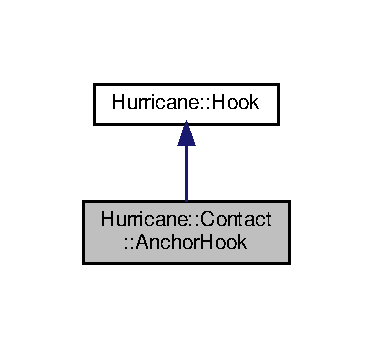
\includegraphics[width=179pt]{classHurricane_1_1Contact_1_1AnchorHook__inherit__graph}
\end{center}
\end{figure}
\doxysubsection*{Additional Inherited Members}


\doxysubsection{Detailed Description}
With contacts, a new type of \mbox{\hyperlink{classHurricane_1_1Hook}{Hook}} appears \+: the {\bfseries{\mbox{\hyperlink{classHurricane_1_1Contact_1_1AnchorHook}{Anchor\+Hook}}}}, which allows to attach a contact upon an other component, on which it is said to be \char`\"{}anchored\char`\"{}. It becomes then a \char`\"{}relative contact\char`\"{} with respect of the coordinates of this component. The \mbox{\hyperlink{classHurricane_1_1Contact_1_1AnchorHook}{Anchor\+Hook}} is always a slave hook.

\begin{DoxyRemark}{Remarks}
A contact has two attributes {\ttfamily $<$Dx$>$} and {\ttfamily $<$Dy$>$} which represent the relative coordinates of the contact with respect to the coordinates of the component on which it is anchored (through this \mbox{\hyperlink{classHurricane_1_1Contact_1_1AnchorHook}{Anchor\+Hook}}). When it is not anchored, those coordinates becomes relative to the origin of the cell, which means they are absolute. 
\end{DoxyRemark}


The documentation for this class was generated from the following file\+:\begin{DoxyCompactItemize}
\item 
Contact.\+h\end{DoxyCompactItemize}

\hypertarget{classHurricane_1_1BasicLayer}{}\doxysection{Hurricane\+::Basic\+Layer Class Reference}
\label{classHurricane_1_1BasicLayer}\index{Hurricane::BasicLayer@{Hurricane::BasicLayer}}


\mbox{\hyperlink{classHurricane_1_1BasicLayer}{Basic\+Layer}} description ({\bfseries{API}})  




Inheritance diagram for Hurricane\+::Basic\+Layer\+:\nopagebreak
\begin{figure}[H]
\begin{center}
\leavevmode
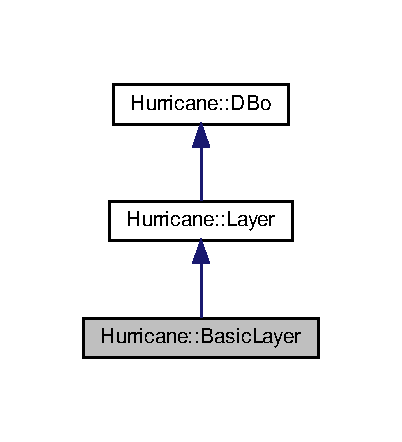
\includegraphics[width=193pt]{classHurricane_1_1BasicLayer__inherit__graph}
\end{center}
\end{figure}
\doxysubsection*{Classes}
\begin{DoxyCompactItemize}
\item 
class \mbox{\hyperlink{classHurricane_1_1BasicLayer_1_1Material}{Material}}
\end{DoxyCompactItemize}
\doxysubsection*{Public Member Functions}
\begin{DoxyCompactItemize}
\item 
const \mbox{\hyperlink{classHurricane_1_1BasicLayer_1_1Material}{Material}} \& \mbox{\hyperlink{classHurricane_1_1BasicLayer_aeb7fd37db4ecf8e56e1992d6350fac58}{get\+Material}} () const
\item 
const \mbox{\hyperlink{classHurricane_1_1Name}{Name}} \& \mbox{\hyperlink{classHurricane_1_1BasicLayer_aaae9fcd776eb83407b4566614eafc41f}{get\+Real\+Name}} () const
\item 
void \mbox{\hyperlink{classHurricane_1_1BasicLayer_a766c6dc1120de2066b15411861f5d4f8}{set\+Blockage\+Layer}} (\mbox{\hyperlink{classHurricane_1_1BasicLayer}{Basic\+Layer}} $\ast$layer)
\item 
void \mbox{\hyperlink{classHurricane_1_1BasicLayer_aa5aa1e1079c14d7e9c05799d14e726af}{set\+Real\+Name}} (const char $\ast$real\+Name)
\end{DoxyCompactItemize}
\doxysubsection*{Static Public Member Functions}
\begin{DoxyCompactItemize}
\item 
static \mbox{\hyperlink{classHurricane_1_1BasicLayer}{Basic\+Layer}} $\ast$ \mbox{\hyperlink{classHurricane_1_1BasicLayer_aecdcb9bef9b3c1c2bcb6d4513e1ca657}{create}} (\mbox{\hyperlink{classHurricane_1_1Technology}{Technology}} $\ast$technology, const \mbox{\hyperlink{classHurricane_1_1Name}{Name}} \&name, const \mbox{\hyperlink{classHurricane_1_1BasicLayer_1_1Material}{Material}} \&material, unsigned gds2\+Layer=0, unsigned gds2\+Datatype=0, const \mbox{\hyperlink{classHurricane_1_1DbU_a4fbfa3e8c89347af76c9628ea06c4146}{Db\+U\+::\+Unit}} \&minimal\+Size=0, const \mbox{\hyperlink{classHurricane_1_1DbU_a4fbfa3e8c89347af76c9628ea06c4146}{Db\+U\+::\+Unit}} \&minimal\+Spacing=0)
\end{DoxyCompactItemize}
\doxysubsection*{Additional Inherited Members}


\doxysubsection{Detailed Description}
\mbox{\hyperlink{classHurricane_1_1BasicLayer}{Basic\+Layer}} description ({\bfseries{API}}) 

For a more complete description of the Layers object, please refer to \mbox{\hyperlink{classHurricane_1_1Layer_secLayerIntro}{Layer Introduction}}.

For purpose of Basic\+Layers, also see \mbox{\hyperlink{classHurricane_1_1BasicLayer_1_1Material}{Basic\+Layer\+::\+Material}}. 

\doxysubsection{Member Function Documentation}
\mbox{\Hypertarget{classHurricane_1_1BasicLayer_aecdcb9bef9b3c1c2bcb6d4513e1ca657}\label{classHurricane_1_1BasicLayer_aecdcb9bef9b3c1c2bcb6d4513e1ca657}} 
\index{Hurricane::BasicLayer@{Hurricane::BasicLayer}!create@{create}}
\index{create@{create}!Hurricane::BasicLayer@{Hurricane::BasicLayer}}
\doxysubsubsection{\texorpdfstring{create()}{create()}}
{\footnotesize\ttfamily \mbox{\hyperlink{classHurricane_1_1BasicLayer}{Basic\+Layer}} $\ast$ Hurricane\+::\+Basic\+Layer\+::create (\begin{DoxyParamCaption}\item[{\mbox{\hyperlink{classHurricane_1_1Technology}{Technology}} $\ast$}]{technology,  }\item[{const \mbox{\hyperlink{classHurricane_1_1Name}{Name}} \&}]{name,  }\item[{const \mbox{\hyperlink{classHurricane_1_1BasicLayer_1_1Material}{Material}} \&}]{material,  }\item[{unsigned}]{gds2\+Layer = {\ttfamily 0},  }\item[{unsigned}]{gds2\+Datatype = {\ttfamily 0},  }\item[{const \mbox{\hyperlink{classHurricane_1_1DbU_a4fbfa3e8c89347af76c9628ea06c4146}{Db\+U\+::\+Unit}} \&}]{minimal\+Size = {\ttfamily 0},  }\item[{const \mbox{\hyperlink{classHurricane_1_1DbU_a4fbfa3e8c89347af76c9628ea06c4146}{Db\+U\+::\+Unit}} \&}]{minimal\+Spacing = {\ttfamily 0} }\end{DoxyParamCaption})\hspace{0.3cm}{\ttfamily [static]}}

creates and returns a new basic layer named {\ttfamily $<$name$>$}, of type {\ttfamily $<$material$>$} for the given technology (some geometrical characteristics can also be specified).

\begin{DoxyParagraph}{Caution\+: Throws an exception if the technology is null, if the name is }
empty, if a layer of same name already exists or if we overflow the capacity of the bit field associated to the layer mask.
\end{DoxyParagraph}
\begin{DoxyRemark}{Remarks}
The extract number is a kind of logic number. In example the CP layer which represent a poly layer should have the same extract number as the CPG layer which represent a poly layer used to realize the transistor gates. While extractions process, layers which have the same extract number are considered as equivalents. A null value indicates that the extraction should ignore this layer. 
\end{DoxyRemark}
\mbox{\Hypertarget{classHurricane_1_1BasicLayer_aeb7fd37db4ecf8e56e1992d6350fac58}\label{classHurricane_1_1BasicLayer_aeb7fd37db4ecf8e56e1992d6350fac58}} 
\index{Hurricane::BasicLayer@{Hurricane::BasicLayer}!getMaterial@{getMaterial}}
\index{getMaterial@{getMaterial}!Hurricane::BasicLayer@{Hurricane::BasicLayer}}
\doxysubsubsection{\texorpdfstring{getMaterial()}{getMaterial()}}
{\footnotesize\ttfamily const Basic\+Layer\+::\+Type \& Hurricane\+::\+Basic\+Layer\+::get\+Material (\begin{DoxyParamCaption}{ }\end{DoxyParamCaption}) const\hspace{0.3cm}{\ttfamily [inline]}}

{\bfseries{Returns\+:}} the basic layer material. \mbox{\Hypertarget{classHurricane_1_1BasicLayer_aaae9fcd776eb83407b4566614eafc41f}\label{classHurricane_1_1BasicLayer_aaae9fcd776eb83407b4566614eafc41f}} 
\index{Hurricane::BasicLayer@{Hurricane::BasicLayer}!getRealName@{getRealName}}
\index{getRealName@{getRealName}!Hurricane::BasicLayer@{Hurricane::BasicLayer}}
\doxysubsubsection{\texorpdfstring{getRealName()}{getRealName()}}
{\footnotesize\ttfamily const \mbox{\hyperlink{classHurricane_1_1Name}{Name}} \& Hurricane\+::\+Basic\+Layer\+::get\+Real\+Name (\begin{DoxyParamCaption}{ }\end{DoxyParamCaption}) const\hspace{0.3cm}{\ttfamily [inline]}}

{\bfseries{Returns\+:}} the real (process) layer name, for GDS. \mbox{\Hypertarget{classHurricane_1_1BasicLayer_a766c6dc1120de2066b15411861f5d4f8}\label{classHurricane_1_1BasicLayer_a766c6dc1120de2066b15411861f5d4f8}} 
\index{Hurricane::BasicLayer@{Hurricane::BasicLayer}!setBlockageLayer@{setBlockageLayer}}
\index{setBlockageLayer@{setBlockageLayer}!Hurricane::BasicLayer@{Hurricane::BasicLayer}}
\doxysubsubsection{\texorpdfstring{setBlockageLayer()}{setBlockageLayer()}}
{\footnotesize\ttfamily void Hurricane\+::\+Basic\+Layer\+::set\+Blockage\+Layer (\begin{DoxyParamCaption}\item[{\mbox{\hyperlink{classHurricane_1_1BasicLayer}{Basic\+Layer}} $\ast$}]{layer }\end{DoxyParamCaption})\hspace{0.3cm}{\ttfamily [inline]}}

Associate a blockage layer to this one. This is only meaningful for routing layers (\mbox{\hyperlink{classHurricane_1_1RegularLayer}{Regular\+Layer}}). \mbox{\Hypertarget{classHurricane_1_1BasicLayer_aa5aa1e1079c14d7e9c05799d14e726af}\label{classHurricane_1_1BasicLayer_aa5aa1e1079c14d7e9c05799d14e726af}} 
\index{Hurricane::BasicLayer@{Hurricane::BasicLayer}!setRealName@{setRealName}}
\index{setRealName@{setRealName}!Hurricane::BasicLayer@{Hurricane::BasicLayer}}
\doxysubsubsection{\texorpdfstring{setRealName()}{setRealName()}}
{\footnotesize\ttfamily void Hurricane\+::\+Basic\+Layer\+::set\+Real\+Name (\begin{DoxyParamCaption}\item[{const char $\ast$}]{real\+Name }\end{DoxyParamCaption})\hspace{0.3cm}{\ttfamily [inline]}}

Set the real (process) layer name, for GDS. 

The documentation for this class was generated from the following files\+:\begin{DoxyCompactItemize}
\item 
Basic\+Layer.\+h\item 
Basic\+Layer.\+dox\end{DoxyCompactItemize}

\hypertarget{classHurricane_1_1Component_1_1BodyHook}{}\doxysection{Hurricane\+::Component\+::Body\+Hook Class Reference}
\label{classHurricane_1_1Component_1_1BodyHook}\index{Hurricane::Component::BodyHook@{Hurricane::Component::BodyHook}}


Inheritance diagram for Hurricane\+::Component\+::Body\+Hook\+:\nopagebreak
\begin{figure}[H]
\begin{center}
\leavevmode
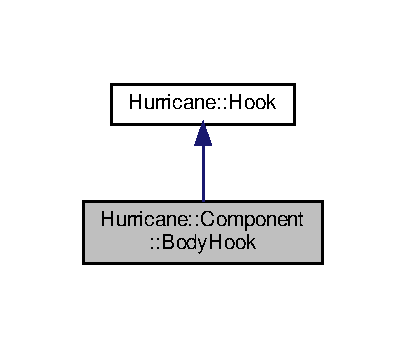
\includegraphics[width=195pt]{classHurricane_1_1Component_1_1BodyHook__inherit__graph}
\end{center}
\end{figure}
\doxysubsection*{Additional Inherited Members}


\doxysubsection{Detailed Description}
With the components, appears a new \mbox{\hyperlink{classHurricane_1_1Hook}{Hook}} type \+: The {\bfseries{\mbox{\hyperlink{classHurricane_1_1Component_1_1BodyHook}{Body\+Hook}}}}, which represents the body of the component inside which it is nested (it is always a {\bfseries{\char`\"{}master\char`\"{}}} hook). 

The documentation for this class was generated from the following file\+:\begin{DoxyCompactItemize}
\item 
Component.\+h\end{DoxyCompactItemize}

\hypertarget{classHurricane_1_1Box}{}\doxysection{Hurricane\+::Box Class Reference}
\label{classHurricane_1_1Box}\index{Hurricane::Box@{Hurricane::Box}}


\mbox{\hyperlink{classHurricane_1_1Box}{Box}} description ({\bfseries{API}})  


\doxysubsection*{Public Member Functions}
\begin{DoxyCompactItemize}
\item 
\mbox{\hyperlink{classHurricane_1_1Box_a445dd24bf83759bb47fc483fc7da024f}{Box}} ()
\item 
\mbox{\hyperlink{classHurricane_1_1Box_af53adb323e9e89eef4e96da9efc33fe9}{Box}} (const \mbox{\hyperlink{classHurricane_1_1DbU_a4fbfa3e8c89347af76c9628ea06c4146}{Db\+U\+::\+Unit}} \&x, const \mbox{\hyperlink{classHurricane_1_1DbU_a4fbfa3e8c89347af76c9628ea06c4146}{Db\+U\+::\+Unit}} \&y)
\item 
\mbox{\hyperlink{classHurricane_1_1Box_a2f2aa57fa9486b508fca2a060648d04a}{Box}} (const \mbox{\hyperlink{classHurricane_1_1Point}{Point}} \&point)
\item 
\mbox{\hyperlink{classHurricane_1_1Box_a101cd5a10d6cf229ccedccbb5417ed55}{Box}} (const \mbox{\hyperlink{classHurricane_1_1DbU_a4fbfa3e8c89347af76c9628ea06c4146}{Db\+U\+::\+Unit}} \&x1, const \mbox{\hyperlink{classHurricane_1_1DbU_a4fbfa3e8c89347af76c9628ea06c4146}{Db\+U\+::\+Unit}} \&y1, const \mbox{\hyperlink{classHurricane_1_1DbU_a4fbfa3e8c89347af76c9628ea06c4146}{Db\+U\+::\+Unit}} \&x2, const \mbox{\hyperlink{classHurricane_1_1DbU_a4fbfa3e8c89347af76c9628ea06c4146}{Db\+U\+::\+Unit}} \&y2)
\item 
\mbox{\hyperlink{classHurricane_1_1Box_a47f434b4dbda6af14a354722f66a47da}{Box}} (const \mbox{\hyperlink{classHurricane_1_1Point}{Point}} \&point1, const \mbox{\hyperlink{classHurricane_1_1Point}{Point}} \&point2)
\item 
\mbox{\hyperlink{classHurricane_1_1Box_af9a7605270bf1ebb38723fba5b9d9236}{Box}} (const \mbox{\hyperlink{classHurricane_1_1Box}{Box}} \&box)
\item 
\mbox{\hyperlink{classHurricane_1_1Box}{Box}} \& \mbox{\hyperlink{classHurricane_1_1Box_a01abf59b3d3e99e694a7d4789f1bb978}{operator=}} (const \mbox{\hyperlink{classHurricane_1_1Box}{Box}} \&box)
\item 
bool \mbox{\hyperlink{classHurricane_1_1Box_a2a363ad0fdfda5a2f56b1b62a8665703}{operator==}} (const \mbox{\hyperlink{classHurricane_1_1Box}{Box}} \&box) const
\item 
bool \mbox{\hyperlink{classHurricane_1_1Box_a77a0e8c424c246973c455ce8e3ada8fb}{operator!=}} (const \mbox{\hyperlink{classHurricane_1_1Box}{Box}} \&box) const
\item 
const \mbox{\hyperlink{classHurricane_1_1DbU_a4fbfa3e8c89347af76c9628ea06c4146}{Db\+U\+::\+Unit}} \& \mbox{\hyperlink{classHurricane_1_1Box_ad5122ef7dda8a58c1dacddb57cd4ccfb}{get\+XMin}} () const
\item 
const \mbox{\hyperlink{classHurricane_1_1DbU_a4fbfa3e8c89347af76c9628ea06c4146}{Db\+U\+::\+Unit}} \& \mbox{\hyperlink{classHurricane_1_1Box_a542c383466845aeca0e32f51b77c7439}{get\+YMin}} () const
\item 
const \mbox{\hyperlink{classHurricane_1_1DbU_a4fbfa3e8c89347af76c9628ea06c4146}{Db\+U\+::\+Unit}} \& \mbox{\hyperlink{classHurricane_1_1Box_a77b9db757080544fcede3e670cee8c5c}{get\+XMax}} () const
\item 
const \mbox{\hyperlink{classHurricane_1_1DbU_a4fbfa3e8c89347af76c9628ea06c4146}{Db\+U\+::\+Unit}} \& \mbox{\hyperlink{classHurricane_1_1Box_a06e1a86a06dacfca6d3403c16affc7e8}{get\+YMax}} () const
\item 
\mbox{\hyperlink{classHurricane_1_1DbU_a4fbfa3e8c89347af76c9628ea06c4146}{Db\+U\+::\+Unit}} \mbox{\hyperlink{classHurricane_1_1Box_a95f35cd33966aad61bb43662306ccf98}{get\+XCenter}} () const
\item 
\mbox{\hyperlink{classHurricane_1_1DbU_a4fbfa3e8c89347af76c9628ea06c4146}{Db\+U\+::\+Unit}} \mbox{\hyperlink{classHurricane_1_1Box_a659820726e3862a70158b6f5b7644da0}{get\+YCenter}} () const
\item 
\mbox{\hyperlink{classHurricane_1_1Point}{Point}} \mbox{\hyperlink{classHurricane_1_1Box_ac18c8725989166d1b101de29531e4f6e}{get\+Center}} () const
\item 
\mbox{\hyperlink{classHurricane_1_1DbU_a4fbfa3e8c89347af76c9628ea06c4146}{Db\+U\+::\+Unit}} \mbox{\hyperlink{classHurricane_1_1Box_ae2cc9cf0b17e6443a88b475bbd36e4c9}{get\+Width}} () const
\item 
\mbox{\hyperlink{classHurricane_1_1DbU_a4fbfa3e8c89347af76c9628ea06c4146}{Db\+U\+::\+Unit}} \mbox{\hyperlink{classHurricane_1_1Box_a8aa689ad799e4c78bfefb0328e7d9081}{get\+Half\+Width}} () const
\item 
\mbox{\hyperlink{classHurricane_1_1DbU_a4fbfa3e8c89347af76c9628ea06c4146}{Db\+U\+::\+Unit}} \mbox{\hyperlink{classHurricane_1_1Box_a7b15b9488d49da1fc666c0383fb213ab}{get\+Height}} () const
\item 
\mbox{\hyperlink{classHurricane_1_1DbU_a4fbfa3e8c89347af76c9628ea06c4146}{Db\+U\+::\+Unit}} \mbox{\hyperlink{classHurricane_1_1Box_a5c94554a78398c4a5c7dedd024926abb}{get\+Half\+Height}} () const
\item 
\mbox{\hyperlink{classHurricane_1_1Box}{Box}} \mbox{\hyperlink{classHurricane_1_1Box_a2670058f109dfae32d284db249e533bc}{get\+Union}} (const \mbox{\hyperlink{classHurricane_1_1Box}{Box}} \&box) const
\item 
\mbox{\hyperlink{classHurricane_1_1Box}{Box}} \mbox{\hyperlink{classHurricane_1_1Box_a610f9c63bc5636ef304f4768215ffb12}{get\+Intersection}} (const \mbox{\hyperlink{classHurricane_1_1Box}{Box}} \&box) const
\item 
bool \mbox{\hyperlink{classHurricane_1_1Box_af8b269603b5c173891a484214ca50266}{is\+Empty}} () const
\item 
bool \mbox{\hyperlink{classHurricane_1_1Box_a0df4d580a3dc1eb23d839c0f53cdee8b}{is\+Flat}} () const
\item 
bool \mbox{\hyperlink{classHurricane_1_1Box_a3d073c5bc3d0ea1b4f21937e36be001f}{is\+Ponctual}} () const
\item 
bool \mbox{\hyperlink{classHurricane_1_1Box_ae18dd30ffbf0b75714ece480f21e2898}{contains}} (const \mbox{\hyperlink{classHurricane_1_1DbU_a4fbfa3e8c89347af76c9628ea06c4146}{Db\+U\+::\+Unit}} \&x, const \mbox{\hyperlink{classHurricane_1_1DbU_a4fbfa3e8c89347af76c9628ea06c4146}{Db\+U\+::\+Unit}} \&y) const
\item 
bool \mbox{\hyperlink{classHurricane_1_1Box_a19ad23904fbfe2afb3683affeb2cac7e}{contains}} (const \mbox{\hyperlink{classHurricane_1_1Point}{Point}} \&point) const
\item 
bool \mbox{\hyperlink{classHurricane_1_1Box_ac567c569f23643e58867afee80f6920a}{contains}} (const \mbox{\hyperlink{classHurricane_1_1Box}{Box}} \&box) const
\item 
bool \mbox{\hyperlink{classHurricane_1_1Box_ae76b57bf6399b29021813da8d3f306ec}{intersect}} (const \mbox{\hyperlink{classHurricane_1_1Box}{Box}} \&box) const
\item 
bool \mbox{\hyperlink{classHurricane_1_1Box_a70d832443d97cb40ec7cb4f0f959a977}{is\+Constrained\+By}} (const \mbox{\hyperlink{classHurricane_1_1Box}{Box}} \&box) const
\item 
\mbox{\hyperlink{classHurricane_1_1Box}{Box}} \& \mbox{\hyperlink{classHurricane_1_1Box_a0717b1b105f65f8284c9b4e36df3a766}{make\+Empty}} ()
\item 
\mbox{\hyperlink{classHurricane_1_1Box}{Box}} \& \mbox{\hyperlink{classHurricane_1_1Box_a90207e7ca8044a6afc72674cc6ae366e}{inflate}} (const \mbox{\hyperlink{classHurricane_1_1DbU_a4fbfa3e8c89347af76c9628ea06c4146}{Db\+U\+::\+Unit}} \&d)
\item 
\mbox{\hyperlink{classHurricane_1_1Box}{Box}} \& \mbox{\hyperlink{classHurricane_1_1Box_a6b97ea9d54fbf4dae52459073cdf4b5f}{inflate}} (const \mbox{\hyperlink{classHurricane_1_1DbU_a4fbfa3e8c89347af76c9628ea06c4146}{Db\+U\+::\+Unit}} \&dx, const \mbox{\hyperlink{classHurricane_1_1DbU_a4fbfa3e8c89347af76c9628ea06c4146}{Db\+U\+::\+Unit}} \&dy)
\item 
\mbox{\hyperlink{classHurricane_1_1Box}{Box}} \& \mbox{\hyperlink{classHurricane_1_1Box_afd1baf9f272878a87c2525f0fa2eab71}{inflate}} (const \mbox{\hyperlink{classHurricane_1_1DbU_a4fbfa3e8c89347af76c9628ea06c4146}{Db\+U\+::\+Unit}} \&dx\+Min, const \mbox{\hyperlink{classHurricane_1_1DbU_a4fbfa3e8c89347af76c9628ea06c4146}{Db\+U\+::\+Unit}} \&dy\+Min, const \mbox{\hyperlink{classHurricane_1_1DbU_a4fbfa3e8c89347af76c9628ea06c4146}{Db\+U\+::\+Unit}} \&dx\+Max, const \mbox{\hyperlink{classHurricane_1_1DbU_a4fbfa3e8c89347af76c9628ea06c4146}{Db\+U\+::\+Unit}} \&dy\+Max)
\item 
\mbox{\hyperlink{classHurricane_1_1Box}{Box}} \& \mbox{\hyperlink{classHurricane_1_1Box_ab77fe56f9350f06cc872bbb4f83835da}{merge}} (const \mbox{\hyperlink{classHurricane_1_1DbU_a4fbfa3e8c89347af76c9628ea06c4146}{Db\+U\+::\+Unit}} \&x, const \mbox{\hyperlink{classHurricane_1_1DbU_a4fbfa3e8c89347af76c9628ea06c4146}{Db\+U\+::\+Unit}} \&y)
\item 
\mbox{\hyperlink{classHurricane_1_1Box}{Box}} \& \mbox{\hyperlink{classHurricane_1_1Box_af1f7dfe8984c2d26fbca78b21358ee2b}{merge}} (const \mbox{\hyperlink{classHurricane_1_1Point}{Point}} \&point)
\item 
\mbox{\hyperlink{classHurricane_1_1Box}{Box}} \& \mbox{\hyperlink{classHurricane_1_1Box_ad97e73e91dd36404eb0dde9d44ff2fd7}{merge}} (const \mbox{\hyperlink{classHurricane_1_1DbU_a4fbfa3e8c89347af76c9628ea06c4146}{Db\+U\+::\+Unit}} \&x1, const \mbox{\hyperlink{classHurricane_1_1DbU_a4fbfa3e8c89347af76c9628ea06c4146}{Db\+U\+::\+Unit}} \&y1, const \mbox{\hyperlink{classHurricane_1_1DbU_a4fbfa3e8c89347af76c9628ea06c4146}{Db\+U\+::\+Unit}} \&x2, const \mbox{\hyperlink{classHurricane_1_1DbU_a4fbfa3e8c89347af76c9628ea06c4146}{Db\+U\+::\+Unit}} \&y2)
\item 
\mbox{\hyperlink{classHurricane_1_1Box}{Box}} \& \mbox{\hyperlink{classHurricane_1_1Box_a0bdfa52a3f5f6639680ba7dbc52c21d7}{merge}} (const \mbox{\hyperlink{classHurricane_1_1Box}{Box}} \&box)
\item 
\mbox{\hyperlink{classHurricane_1_1Box}{Box}} \& \mbox{\hyperlink{classHurricane_1_1Box_aa689be4b37c83412f3dc95fc23c82156}{translate}} (const \mbox{\hyperlink{classHurricane_1_1DbU_a4fbfa3e8c89347af76c9628ea06c4146}{Db\+U\+::\+Unit}} \&dx, const \mbox{\hyperlink{classHurricane_1_1DbU_a4fbfa3e8c89347af76c9628ea06c4146}{Db\+U\+::\+Unit}} \&dy)
\end{DoxyCompactItemize}


\doxysubsection{Detailed Description}
\mbox{\hyperlink{classHurricane_1_1Box}{Box}} description ({\bfseries{API}}) 

\hypertarget{classHurricane_1_1Box_secBoxIntro}{}\doxysubsection{Introduction}\label{classHurricane_1_1Box_secBoxIntro}
Those objects represent rectangular boxes. They are defined by the values {\bfseries{XMin}}, {\bfseries{YMin}}, {\bfseries{XMax}} and {\bfseries{YMax}} which are representatives only when the box is not empty. A box is considered empty whenever it is not initialized or when it doesn\textquotesingle{}t represent a real area like the intersection of two disjoint boxes.\hypertarget{classHurricane_1_1Box_secBoxModifierRemark}{}\doxysubsection{Remark on Modifiers}\label{classHurricane_1_1Box_secBoxModifierRemark}
All the function described in the modifiers section returns a reference on the modified box, providing so the capability to apply to it a new modification as illustrated in the following example \+: 
\begin{DoxyCode}{0}
\DoxyCodeLine{\mbox{\hyperlink{classHurricane_1_1Box_a445dd24bf83759bb47fc483fc7da024f}{Box}} box1(0, 0, 100, 100);}
\DoxyCodeLine{\mbox{\hyperlink{classHurricane_1_1Box_a445dd24bf83759bb47fc483fc7da024f}{Box}} box2(20, 20, 50, 150;}
\DoxyCodeLine{ }
\DoxyCodeLine{\textcolor{keywordflow}{if} (box1.inflate(3).merge(box2.translate(10, 10).inflate(-\/1, 1)).contains(20, 20)) \{}
\DoxyCodeLine{   \textcolor{comment}{// do we reach here ? that is the question !}}
\DoxyCodeLine{\}}

\end{DoxyCode}
 

\doxysubsection{Constructor \& Destructor Documentation}
\mbox{\Hypertarget{classHurricane_1_1Box_a445dd24bf83759bb47fc483fc7da024f}\label{classHurricane_1_1Box_a445dd24bf83759bb47fc483fc7da024f}} 
\index{Hurricane::Box@{Hurricane::Box}!Box@{Box}}
\index{Box@{Box}!Hurricane::Box@{Hurricane::Box}}
\doxysubsubsection{\texorpdfstring{Box()}{Box()}\hspace{0.1cm}{\footnotesize\ttfamily [1/6]}}
{\footnotesize\ttfamily Hurricane\+::\+Box\+::\+Box (\begin{DoxyParamCaption}{ }\end{DoxyParamCaption})}

Default constructor \+: the returned box is empty. \mbox{\Hypertarget{classHurricane_1_1Box_af53adb323e9e89eef4e96da9efc33fe9}\label{classHurricane_1_1Box_af53adb323e9e89eef4e96da9efc33fe9}} 
\index{Hurricane::Box@{Hurricane::Box}!Box@{Box}}
\index{Box@{Box}!Hurricane::Box@{Hurricane::Box}}
\doxysubsubsection{\texorpdfstring{Box()}{Box()}\hspace{0.1cm}{\footnotesize\ttfamily [2/6]}}
{\footnotesize\ttfamily Hurricane\+::\+Box\+::\+Box (\begin{DoxyParamCaption}\item[{const \mbox{\hyperlink{classHurricane_1_1DbU_a4fbfa3e8c89347af76c9628ea06c4146}{Db\+U\+::\+Unit}} \&}]{x,  }\item[{const \mbox{\hyperlink{classHurricane_1_1DbU_a4fbfa3e8c89347af76c9628ea06c4146}{Db\+U\+::\+Unit}} \&}]{y }\end{DoxyParamCaption})}

Builds a box of null size centered on the point defined by {\ttfamily $<$x$>$} and {\ttfamily $<$y$>$}. \mbox{\Hypertarget{classHurricane_1_1Box_a2f2aa57fa9486b508fca2a060648d04a}\label{classHurricane_1_1Box_a2f2aa57fa9486b508fca2a060648d04a}} 
\index{Hurricane::Box@{Hurricane::Box}!Box@{Box}}
\index{Box@{Box}!Hurricane::Box@{Hurricane::Box}}
\doxysubsubsection{\texorpdfstring{Box()}{Box()}\hspace{0.1cm}{\footnotesize\ttfamily [3/6]}}
{\footnotesize\ttfamily Hurricane\+::\+Box\+::\+Box (\begin{DoxyParamCaption}\item[{const \mbox{\hyperlink{classHurricane_1_1Point}{Point}} \&}]{point }\end{DoxyParamCaption})}

Builds a box of null size centered on the point. \mbox{\Hypertarget{classHurricane_1_1Box_a101cd5a10d6cf229ccedccbb5417ed55}\label{classHurricane_1_1Box_a101cd5a10d6cf229ccedccbb5417ed55}} 
\index{Hurricane::Box@{Hurricane::Box}!Box@{Box}}
\index{Box@{Box}!Hurricane::Box@{Hurricane::Box}}
\doxysubsubsection{\texorpdfstring{Box()}{Box()}\hspace{0.1cm}{\footnotesize\ttfamily [4/6]}}
{\footnotesize\ttfamily Hurricane\+::\+Box\+::\+Box (\begin{DoxyParamCaption}\item[{const \mbox{\hyperlink{classHurricane_1_1DbU_a4fbfa3e8c89347af76c9628ea06c4146}{Db\+U\+::\+Unit}} \&}]{x1,  }\item[{const \mbox{\hyperlink{classHurricane_1_1DbU_a4fbfa3e8c89347af76c9628ea06c4146}{Db\+U\+::\+Unit}} \&}]{y1,  }\item[{const \mbox{\hyperlink{classHurricane_1_1DbU_a4fbfa3e8c89347af76c9628ea06c4146}{Db\+U\+::\+Unit}} \&}]{x2,  }\item[{const \mbox{\hyperlink{classHurricane_1_1DbU_a4fbfa3e8c89347af76c9628ea06c4146}{Db\+U\+::\+Unit}} \&}]{y2 }\end{DoxyParamCaption})}

Builds the minimal box enclosing the two points defined by the coordinates {\ttfamily $<$x1$>$}, {\ttfamily $<$y1$>$} and {\ttfamily $<$x2$>$}, {\ttfamily $<$y2$>$}. \mbox{\Hypertarget{classHurricane_1_1Box_a47f434b4dbda6af14a354722f66a47da}\label{classHurricane_1_1Box_a47f434b4dbda6af14a354722f66a47da}} 
\index{Hurricane::Box@{Hurricane::Box}!Box@{Box}}
\index{Box@{Box}!Hurricane::Box@{Hurricane::Box}}
\doxysubsubsection{\texorpdfstring{Box()}{Box()}\hspace{0.1cm}{\footnotesize\ttfamily [5/6]}}
{\footnotesize\ttfamily Hurricane\+::\+Box\+::\+Box (\begin{DoxyParamCaption}\item[{const \mbox{\hyperlink{classHurricane_1_1Point}{Point}} \&}]{point1,  }\item[{const \mbox{\hyperlink{classHurricane_1_1Point}{Point}} \&}]{point2 }\end{DoxyParamCaption})}

Builds the minimal box enclosing the two points. \mbox{\Hypertarget{classHurricane_1_1Box_af9a7605270bf1ebb38723fba5b9d9236}\label{classHurricane_1_1Box_af9a7605270bf1ebb38723fba5b9d9236}} 
\index{Hurricane::Box@{Hurricane::Box}!Box@{Box}}
\index{Box@{Box}!Hurricane::Box@{Hurricane::Box}}
\doxysubsubsection{\texorpdfstring{Box()}{Box()}\hspace{0.1cm}{\footnotesize\ttfamily [6/6]}}
{\footnotesize\ttfamily Hurricane\+::\+Box\+::\+Box (\begin{DoxyParamCaption}\item[{const \mbox{\hyperlink{classHurricane_1_1Box}{Box}} \&}]{box }\end{DoxyParamCaption})}

Copy constructor. 

\doxysubsection{Member Function Documentation}
\mbox{\Hypertarget{classHurricane_1_1Box_a01abf59b3d3e99e694a7d4789f1bb978}\label{classHurricane_1_1Box_a01abf59b3d3e99e694a7d4789f1bb978}} 
\index{Hurricane::Box@{Hurricane::Box}!operator=@{operator=}}
\index{operator=@{operator=}!Hurricane::Box@{Hurricane::Box}}
\doxysubsubsection{\texorpdfstring{operator=()}{operator=()}}
{\footnotesize\ttfamily \mbox{\hyperlink{classHurricane_1_1Box}{Box}} \& Hurricane\+::\+Box\+::operator= (\begin{DoxyParamCaption}\item[{const \mbox{\hyperlink{classHurricane_1_1Box}{Box}} \&}]{box }\end{DoxyParamCaption})}

Assignment operator. \mbox{\Hypertarget{classHurricane_1_1Box_a2a363ad0fdfda5a2f56b1b62a8665703}\label{classHurricane_1_1Box_a2a363ad0fdfda5a2f56b1b62a8665703}} 
\index{Hurricane::Box@{Hurricane::Box}!operator==@{operator==}}
\index{operator==@{operator==}!Hurricane::Box@{Hurricane::Box}}
\doxysubsubsection{\texorpdfstring{operator==()}{operator==()}}
{\footnotesize\ttfamily bool Hurricane\+::\+Box\+::operator== (\begin{DoxyParamCaption}\item[{const \mbox{\hyperlink{classHurricane_1_1Box}{Box}} \&}]{box }\end{DoxyParamCaption}) const}

Equality operator.

\begin{DoxyRemark}{Remarks}
Two empty boxes are always different. 
\end{DoxyRemark}
\mbox{\Hypertarget{classHurricane_1_1Box_a77a0e8c424c246973c455ce8e3ada8fb}\label{classHurricane_1_1Box_a77a0e8c424c246973c455ce8e3ada8fb}} 
\index{Hurricane::Box@{Hurricane::Box}!operator"!=@{operator"!=}}
\index{operator"!=@{operator"!=}!Hurricane::Box@{Hurricane::Box}}
\doxysubsubsection{\texorpdfstring{operator"!=()}{operator!=()}}
{\footnotesize\ttfamily bool Hurricane\+::\+Box\+::operator!= (\begin{DoxyParamCaption}\item[{const \mbox{\hyperlink{classHurricane_1_1Box}{Box}} \&}]{box }\end{DoxyParamCaption}) const}

Difference operator. \mbox{\Hypertarget{classHurricane_1_1Box_ad5122ef7dda8a58c1dacddb57cd4ccfb}\label{classHurricane_1_1Box_ad5122ef7dda8a58c1dacddb57cd4ccfb}} 
\index{Hurricane::Box@{Hurricane::Box}!getXMin@{getXMin}}
\index{getXMin@{getXMin}!Hurricane::Box@{Hurricane::Box}}
\doxysubsubsection{\texorpdfstring{getXMin()}{getXMin()}}
{\footnotesize\ttfamily const \mbox{\hyperlink{classHurricane_1_1DbU_a4fbfa3e8c89347af76c9628ea06c4146}{Db\+U\+::\+Unit}} \& Hurricane\+::\+Box\+::get\+XMin (\begin{DoxyParamCaption}{ }\end{DoxyParamCaption}) const\hspace{0.3cm}{\ttfamily [inline]}}

{\bfseries{Returns\+:}} the XMin value \+: meaningful only for a non empty box. \mbox{\Hypertarget{classHurricane_1_1Box_a542c383466845aeca0e32f51b77c7439}\label{classHurricane_1_1Box_a542c383466845aeca0e32f51b77c7439}} 
\index{Hurricane::Box@{Hurricane::Box}!getYMin@{getYMin}}
\index{getYMin@{getYMin}!Hurricane::Box@{Hurricane::Box}}
\doxysubsubsection{\texorpdfstring{getYMin()}{getYMin()}}
{\footnotesize\ttfamily const \mbox{\hyperlink{classHurricane_1_1DbU_a4fbfa3e8c89347af76c9628ea06c4146}{Db\+U\+::\+Unit}} \& Hurricane\+::\+Box\+::get\+YMin (\begin{DoxyParamCaption}{ }\end{DoxyParamCaption}) const\hspace{0.3cm}{\ttfamily [inline]}}

{\bfseries{Returns\+:}} the YMin value \+: meaningful only for a non empty box. \mbox{\Hypertarget{classHurricane_1_1Box_a77b9db757080544fcede3e670cee8c5c}\label{classHurricane_1_1Box_a77b9db757080544fcede3e670cee8c5c}} 
\index{Hurricane::Box@{Hurricane::Box}!getXMax@{getXMax}}
\index{getXMax@{getXMax}!Hurricane::Box@{Hurricane::Box}}
\doxysubsubsection{\texorpdfstring{getXMax()}{getXMax()}}
{\footnotesize\ttfamily const \mbox{\hyperlink{classHurricane_1_1DbU_a4fbfa3e8c89347af76c9628ea06c4146}{Db\+U\+::\+Unit}} \& Hurricane\+::\+Box\+::get\+XMax (\begin{DoxyParamCaption}{ }\end{DoxyParamCaption}) const\hspace{0.3cm}{\ttfamily [inline]}}

{\bfseries{Returns\+:}} the XMax value \+: meaningful only for a non empty box. \mbox{\Hypertarget{classHurricane_1_1Box_a06e1a86a06dacfca6d3403c16affc7e8}\label{classHurricane_1_1Box_a06e1a86a06dacfca6d3403c16affc7e8}} 
\index{Hurricane::Box@{Hurricane::Box}!getYMax@{getYMax}}
\index{getYMax@{getYMax}!Hurricane::Box@{Hurricane::Box}}
\doxysubsubsection{\texorpdfstring{getYMax()}{getYMax()}}
{\footnotesize\ttfamily const \mbox{\hyperlink{classHurricane_1_1DbU_a4fbfa3e8c89347af76c9628ea06c4146}{Db\+U\+::\+Unit}} \& Hurricane\+::\+Box\+::get\+YMax (\begin{DoxyParamCaption}{ }\end{DoxyParamCaption}) const\hspace{0.3cm}{\ttfamily [inline]}}

{\bfseries{Returns\+:}} the YMax value \+: meaningful only for a non empty box. \mbox{\Hypertarget{classHurricane_1_1Box_a95f35cd33966aad61bb43662306ccf98}\label{classHurricane_1_1Box_a95f35cd33966aad61bb43662306ccf98}} 
\index{Hurricane::Box@{Hurricane::Box}!getXCenter@{getXCenter}}
\index{getXCenter@{getXCenter}!Hurricane::Box@{Hurricane::Box}}
\doxysubsubsection{\texorpdfstring{getXCenter()}{getXCenter()}}
{\footnotesize\ttfamily \mbox{\hyperlink{classHurricane_1_1DbU_a4fbfa3e8c89347af76c9628ea06c4146}{Db\+U\+::\+Unit}} Hurricane\+::\+Box\+::get\+XCenter (\begin{DoxyParamCaption}{ }\end{DoxyParamCaption}) const\hspace{0.3cm}{\ttfamily [inline]}}

{\bfseries{Returns\+:}} the abscissa of the box center \+: meaningful only for a non empty box. 

Referenced by get\+Center().

\mbox{\Hypertarget{classHurricane_1_1Box_a659820726e3862a70158b6f5b7644da0}\label{classHurricane_1_1Box_a659820726e3862a70158b6f5b7644da0}} 
\index{Hurricane::Box@{Hurricane::Box}!getYCenter@{getYCenter}}
\index{getYCenter@{getYCenter}!Hurricane::Box@{Hurricane::Box}}
\doxysubsubsection{\texorpdfstring{getYCenter()}{getYCenter()}}
{\footnotesize\ttfamily \mbox{\hyperlink{classHurricane_1_1DbU_a4fbfa3e8c89347af76c9628ea06c4146}{Db\+U\+::\+Unit}} Hurricane\+::\+Box\+::get\+YCenter (\begin{DoxyParamCaption}{ }\end{DoxyParamCaption}) const\hspace{0.3cm}{\ttfamily [inline]}}

{\bfseries{Returns\+:}} the ordinate of the box center \+: meaningful only for a non empty box. 

Referenced by get\+Center().

\mbox{\Hypertarget{classHurricane_1_1Box_ac18c8725989166d1b101de29531e4f6e}\label{classHurricane_1_1Box_ac18c8725989166d1b101de29531e4f6e}} 
\index{Hurricane::Box@{Hurricane::Box}!getCenter@{getCenter}}
\index{getCenter@{getCenter}!Hurricane::Box@{Hurricane::Box}}
\doxysubsubsection{\texorpdfstring{getCenter()}{getCenter()}}
{\footnotesize\ttfamily \mbox{\hyperlink{classHurricane_1_1Point}{Point}} Hurricane\+::\+Box\+::get\+Center (\begin{DoxyParamCaption}{ }\end{DoxyParamCaption}) const\hspace{0.3cm}{\ttfamily [inline]}}

{\bfseries{Returns\+:}} the box center point \+: meaningful only for a non empty box. 

References get\+XCenter(), and get\+YCenter().

\mbox{\Hypertarget{classHurricane_1_1Box_ae2cc9cf0b17e6443a88b475bbd36e4c9}\label{classHurricane_1_1Box_ae2cc9cf0b17e6443a88b475bbd36e4c9}} 
\index{Hurricane::Box@{Hurricane::Box}!getWidth@{getWidth}}
\index{getWidth@{getWidth}!Hurricane::Box@{Hurricane::Box}}
\doxysubsubsection{\texorpdfstring{getWidth()}{getWidth()}}
{\footnotesize\ttfamily \mbox{\hyperlink{classHurricane_1_1DbU_a4fbfa3e8c89347af76c9628ea06c4146}{Db\+U\+::\+Unit}} Hurricane\+::\+Box\+::get\+Width (\begin{DoxyParamCaption}{ }\end{DoxyParamCaption}) const\hspace{0.3cm}{\ttfamily [inline]}}

{\bfseries{Returns\+:}} the box width \+: meaningful only for a non empty box. 

Referenced by get\+Half\+Width().

\mbox{\Hypertarget{classHurricane_1_1Box_a8aa689ad799e4c78bfefb0328e7d9081}\label{classHurricane_1_1Box_a8aa689ad799e4c78bfefb0328e7d9081}} 
\index{Hurricane::Box@{Hurricane::Box}!getHalfWidth@{getHalfWidth}}
\index{getHalfWidth@{getHalfWidth}!Hurricane::Box@{Hurricane::Box}}
\doxysubsubsection{\texorpdfstring{getHalfWidth()}{getHalfWidth()}}
{\footnotesize\ttfamily \mbox{\hyperlink{classHurricane_1_1DbU_a4fbfa3e8c89347af76c9628ea06c4146}{Db\+U\+::\+Unit}} Hurricane\+::\+Box\+::get\+Half\+Width (\begin{DoxyParamCaption}{ }\end{DoxyParamCaption}) const\hspace{0.3cm}{\ttfamily [inline]}}

{\bfseries{Returns\+:}} the half box width \+: meaningful only for a non empty box. 

References get\+Width().

\mbox{\Hypertarget{classHurricane_1_1Box_a7b15b9488d49da1fc666c0383fb213ab}\label{classHurricane_1_1Box_a7b15b9488d49da1fc666c0383fb213ab}} 
\index{Hurricane::Box@{Hurricane::Box}!getHeight@{getHeight}}
\index{getHeight@{getHeight}!Hurricane::Box@{Hurricane::Box}}
\doxysubsubsection{\texorpdfstring{getHeight()}{getHeight()}}
{\footnotesize\ttfamily \mbox{\hyperlink{classHurricane_1_1DbU_a4fbfa3e8c89347af76c9628ea06c4146}{Db\+U\+::\+Unit}} Hurricane\+::\+Box\+::get\+Height (\begin{DoxyParamCaption}{ }\end{DoxyParamCaption}) const\hspace{0.3cm}{\ttfamily [inline]}}

{\bfseries{Returns\+:}} the box height \+: meaningful only for a non empty box. 

Referenced by get\+Half\+Height().

\mbox{\Hypertarget{classHurricane_1_1Box_a5c94554a78398c4a5c7dedd024926abb}\label{classHurricane_1_1Box_a5c94554a78398c4a5c7dedd024926abb}} 
\index{Hurricane::Box@{Hurricane::Box}!getHalfHeight@{getHalfHeight}}
\index{getHalfHeight@{getHalfHeight}!Hurricane::Box@{Hurricane::Box}}
\doxysubsubsection{\texorpdfstring{getHalfHeight()}{getHalfHeight()}}
{\footnotesize\ttfamily \mbox{\hyperlink{classHurricane_1_1DbU_a4fbfa3e8c89347af76c9628ea06c4146}{Db\+U\+::\+Unit}} Hurricane\+::\+Box\+::get\+Half\+Height (\begin{DoxyParamCaption}{ }\end{DoxyParamCaption}) const\hspace{0.3cm}{\ttfamily [inline]}}

{\bfseries{Returns\+:}} the half box height \+: meaningful only for a non empty box. 

References get\+Height().

\mbox{\Hypertarget{classHurricane_1_1Box_a2670058f109dfae32d284db249e533bc}\label{classHurricane_1_1Box_a2670058f109dfae32d284db249e533bc}} 
\index{Hurricane::Box@{Hurricane::Box}!getUnion@{getUnion}}
\index{getUnion@{getUnion}!Hurricane::Box@{Hurricane::Box}}
\doxysubsubsection{\texorpdfstring{getUnion()}{getUnion()}}
{\footnotesize\ttfamily \mbox{\hyperlink{classHurricane_1_1Box}{Box}} Hurricane\+::\+Box\+::get\+Union (\begin{DoxyParamCaption}\item[{const \mbox{\hyperlink{classHurricane_1_1Box}{Box}} \&}]{box }\end{DoxyParamCaption}) const}

{\bfseries{Returns\+:}} the smallest enclosing box containing the boxes {\ttfamily $<$this$>$} and {\ttfamily $<$box$>$}. The returned box may be empty if both are. \mbox{\Hypertarget{classHurricane_1_1Box_a610f9c63bc5636ef304f4768215ffb12}\label{classHurricane_1_1Box_a610f9c63bc5636ef304f4768215ffb12}} 
\index{Hurricane::Box@{Hurricane::Box}!getIntersection@{getIntersection}}
\index{getIntersection@{getIntersection}!Hurricane::Box@{Hurricane::Box}}
\doxysubsubsection{\texorpdfstring{getIntersection()}{getIntersection()}}
{\footnotesize\ttfamily \mbox{\hyperlink{classHurricane_1_1Box}{Box}} Hurricane\+::\+Box\+::get\+Intersection (\begin{DoxyParamCaption}\item[{const \mbox{\hyperlink{classHurricane_1_1Box}{Box}} \&}]{box }\end{DoxyParamCaption}) const}

{\bfseries{Returns\+:}} box representing the overlapping area. This box is empty if either one of the two boxes is empty or if they are disjoint. \mbox{\Hypertarget{classHurricane_1_1Box_af8b269603b5c173891a484214ca50266}\label{classHurricane_1_1Box_af8b269603b5c173891a484214ca50266}} 
\index{Hurricane::Box@{Hurricane::Box}!isEmpty@{isEmpty}}
\index{isEmpty@{isEmpty}!Hurricane::Box@{Hurricane::Box}}
\doxysubsubsection{\texorpdfstring{isEmpty()}{isEmpty()}}
{\footnotesize\ttfamily bool Hurricane\+::\+Box\+::is\+Empty (\begin{DoxyParamCaption}{ }\end{DoxyParamCaption}) const}

{\bfseries{Returns\+:}} {\bfseries{true}} if the box is empty, else {\bfseries{false}}. \mbox{\Hypertarget{classHurricane_1_1Box_a0df4d580a3dc1eb23d839c0f53cdee8b}\label{classHurricane_1_1Box_a0df4d580a3dc1eb23d839c0f53cdee8b}} 
\index{Hurricane::Box@{Hurricane::Box}!isFlat@{isFlat}}
\index{isFlat@{isFlat}!Hurricane::Box@{Hurricane::Box}}
\doxysubsubsection{\texorpdfstring{isFlat()}{isFlat()}}
{\footnotesize\ttfamily bool Hurricane\+::\+Box\+::is\+Flat (\begin{DoxyParamCaption}{ }\end{DoxyParamCaption}) const}

{\bfseries{Returns\+:}} {\bfseries{true}} if the box is non void and if we have either ((XMin==XMax) an (YMin$<$YMax)) or ((XMin$<$XMax) and (YMin==YMax)). \mbox{\Hypertarget{classHurricane_1_1Box_a3d073c5bc3d0ea1b4f21937e36be001f}\label{classHurricane_1_1Box_a3d073c5bc3d0ea1b4f21937e36be001f}} 
\index{Hurricane::Box@{Hurricane::Box}!isPonctual@{isPonctual}}
\index{isPonctual@{isPonctual}!Hurricane::Box@{Hurricane::Box}}
\doxysubsubsection{\texorpdfstring{isPonctual()}{isPonctual()}}
{\footnotesize\ttfamily bool Hurricane\+::\+Box\+::is\+Ponctual (\begin{DoxyParamCaption}{ }\end{DoxyParamCaption}) const}

{\bfseries{Returns\+:}} {\bfseries{true}} if the box is reduced to a point, else {\bfseries{false}}. \mbox{\Hypertarget{classHurricane_1_1Box_ae18dd30ffbf0b75714ece480f21e2898}\label{classHurricane_1_1Box_ae18dd30ffbf0b75714ece480f21e2898}} 
\index{Hurricane::Box@{Hurricane::Box}!contains@{contains}}
\index{contains@{contains}!Hurricane::Box@{Hurricane::Box}}
\doxysubsubsection{\texorpdfstring{contains()}{contains()}\hspace{0.1cm}{\footnotesize\ttfamily [1/3]}}
{\footnotesize\ttfamily bool Hurricane\+::\+Box\+::contains (\begin{DoxyParamCaption}\item[{const \mbox{\hyperlink{classHurricane_1_1DbU_a4fbfa3e8c89347af76c9628ea06c4146}{Db\+U\+::\+Unit}} \&}]{x,  }\item[{const \mbox{\hyperlink{classHurricane_1_1DbU_a4fbfa3e8c89347af76c9628ea06c4146}{Db\+U\+::\+Unit}} \&}]{y }\end{DoxyParamCaption}) const}

{\bfseries{Returns\+:}} {\bfseries{true}} if the box is non empty and contains the point defined by the coordinates {\ttfamily $<$x$>$}, {\ttfamily $<$y$>$} else {\bfseries{false}}. \mbox{\Hypertarget{classHurricane_1_1Box_a19ad23904fbfe2afb3683affeb2cac7e}\label{classHurricane_1_1Box_a19ad23904fbfe2afb3683affeb2cac7e}} 
\index{Hurricane::Box@{Hurricane::Box}!contains@{contains}}
\index{contains@{contains}!Hurricane::Box@{Hurricane::Box}}
\doxysubsubsection{\texorpdfstring{contains()}{contains()}\hspace{0.1cm}{\footnotesize\ttfamily [2/3]}}
{\footnotesize\ttfamily bool Hurricane\+::\+Box\+::contains (\begin{DoxyParamCaption}\item[{const \mbox{\hyperlink{classHurricane_1_1Point}{Point}} \&}]{point }\end{DoxyParamCaption}) const}

{\bfseries{Returns\+:}} {\bfseries{true}} if the box is non empty and contains the point {\ttfamily $<$point$>$}, else {\bfseries{false}}. \mbox{\Hypertarget{classHurricane_1_1Box_ac567c569f23643e58867afee80f6920a}\label{classHurricane_1_1Box_ac567c569f23643e58867afee80f6920a}} 
\index{Hurricane::Box@{Hurricane::Box}!contains@{contains}}
\index{contains@{contains}!Hurricane::Box@{Hurricane::Box}}
\doxysubsubsection{\texorpdfstring{contains()}{contains()}\hspace{0.1cm}{\footnotesize\ttfamily [3/3]}}
{\footnotesize\ttfamily bool Hurricane\+::\+Box\+::contains (\begin{DoxyParamCaption}\item[{const \mbox{\hyperlink{classHurricane_1_1Box}{Box}} \&}]{box }\end{DoxyParamCaption}) const}

{\bfseries{Returns\+:}} {\bfseries{true}} if the two boxes are non empty and if the box {\ttfamily $<$this$>$} contains the box {\ttfamily $<$box$>$}, else {\bfseries{false}}. \mbox{\Hypertarget{classHurricane_1_1Box_ae76b57bf6399b29021813da8d3f306ec}\label{classHurricane_1_1Box_ae76b57bf6399b29021813da8d3f306ec}} 
\index{Hurricane::Box@{Hurricane::Box}!intersect@{intersect}}
\index{intersect@{intersect}!Hurricane::Box@{Hurricane::Box}}
\doxysubsubsection{\texorpdfstring{intersect()}{intersect()}}
{\footnotesize\ttfamily bool Hurricane\+::\+Box\+::intersect (\begin{DoxyParamCaption}\item[{const \mbox{\hyperlink{classHurricane_1_1Box}{Box}} \&}]{box }\end{DoxyParamCaption}) const}

{\bfseries{Returns\+:}} {\bfseries{true}} if the two boxes are non empty and if they overlap, else {\bfseries{false}}. \mbox{\Hypertarget{classHurricane_1_1Box_a70d832443d97cb40ec7cb4f0f959a977}\label{classHurricane_1_1Box_a70d832443d97cb40ec7cb4f0f959a977}} 
\index{Hurricane::Box@{Hurricane::Box}!isConstrainedBy@{isConstrainedBy}}
\index{isConstrainedBy@{isConstrainedBy}!Hurricane::Box@{Hurricane::Box}}
\doxysubsubsection{\texorpdfstring{isConstrainedBy()}{isConstrainedBy()}}
{\footnotesize\ttfamily bool Hurricane\+::\+Box\+::is\+Constrained\+By (\begin{DoxyParamCaption}\item[{const \mbox{\hyperlink{classHurricane_1_1Box}{Box}} \&}]{box }\end{DoxyParamCaption}) const}

{\bfseries{Returns\+:}} {\bfseries{true}} if the two boxes are non empty, if the box {\ttfamily $<$this$>$} contains the box {\ttfamily $<$box$>$} and if those two boxes have at least a common border side, else {\bfseries{false}}. \mbox{\Hypertarget{classHurricane_1_1Box_a0717b1b105f65f8284c9b4e36df3a766}\label{classHurricane_1_1Box_a0717b1b105f65f8284c9b4e36df3a766}} 
\index{Hurricane::Box@{Hurricane::Box}!makeEmpty@{makeEmpty}}
\index{makeEmpty@{makeEmpty}!Hurricane::Box@{Hurricane::Box}}
\doxysubsubsection{\texorpdfstring{makeEmpty()}{makeEmpty()}}
{\footnotesize\ttfamily \mbox{\hyperlink{classHurricane_1_1Box}{Box}} \& Hurricane\+::\+Box\+::make\+Empty (\begin{DoxyParamCaption}{ }\end{DoxyParamCaption})}

Transforms the box into an empty one. \mbox{\Hypertarget{classHurricane_1_1Box_a90207e7ca8044a6afc72674cc6ae366e}\label{classHurricane_1_1Box_a90207e7ca8044a6afc72674cc6ae366e}} 
\index{Hurricane::Box@{Hurricane::Box}!inflate@{inflate}}
\index{inflate@{inflate}!Hurricane::Box@{Hurricane::Box}}
\doxysubsubsection{\texorpdfstring{inflate()}{inflate()}\hspace{0.1cm}{\footnotesize\ttfamily [1/3]}}
{\footnotesize\ttfamily \mbox{\hyperlink{classHurricane_1_1Box}{Box}} \& Hurricane\+::\+Box\+::inflate (\begin{DoxyParamCaption}\item[{const \mbox{\hyperlink{classHurricane_1_1DbU_a4fbfa3e8c89347af76c9628ea06c4146}{Db\+U\+::\+Unit}} \&}]{d }\end{DoxyParamCaption})}

Expands (or contracts) the box, if not empty, in each direction of the quantity {\ttfamily $<$d$>$}. This quantity might be negative enough to transform it into an empty box. \mbox{\Hypertarget{classHurricane_1_1Box_a6b97ea9d54fbf4dae52459073cdf4b5f}\label{classHurricane_1_1Box_a6b97ea9d54fbf4dae52459073cdf4b5f}} 
\index{Hurricane::Box@{Hurricane::Box}!inflate@{inflate}}
\index{inflate@{inflate}!Hurricane::Box@{Hurricane::Box}}
\doxysubsubsection{\texorpdfstring{inflate()}{inflate()}\hspace{0.1cm}{\footnotesize\ttfamily [2/3]}}
{\footnotesize\ttfamily \mbox{\hyperlink{classHurricane_1_1Box}{Box}} \& Hurricane\+::\+Box\+::inflate (\begin{DoxyParamCaption}\item[{const \mbox{\hyperlink{classHurricane_1_1DbU_a4fbfa3e8c89347af76c9628ea06c4146}{Db\+U\+::\+Unit}} \&}]{dx,  }\item[{const \mbox{\hyperlink{classHurricane_1_1DbU_a4fbfa3e8c89347af76c9628ea06c4146}{Db\+U\+::\+Unit}} \&}]{dy }\end{DoxyParamCaption})}

Expands (or contracts) the box, if not empty, horizontaly of the quantity {\ttfamily $<$dx$>$} and vertically of the quatity {\ttfamily $<$dy$>$}. Those quantities might be negative enough to transform it into an empty box. \mbox{\Hypertarget{classHurricane_1_1Box_afd1baf9f272878a87c2525f0fa2eab71}\label{classHurricane_1_1Box_afd1baf9f272878a87c2525f0fa2eab71}} 
\index{Hurricane::Box@{Hurricane::Box}!inflate@{inflate}}
\index{inflate@{inflate}!Hurricane::Box@{Hurricane::Box}}
\doxysubsubsection{\texorpdfstring{inflate()}{inflate()}\hspace{0.1cm}{\footnotesize\ttfamily [3/3]}}
{\footnotesize\ttfamily \mbox{\hyperlink{classHurricane_1_1Box}{Box}} \& Hurricane\+::\+Box\+::inflate (\begin{DoxyParamCaption}\item[{const \mbox{\hyperlink{classHurricane_1_1DbU_a4fbfa3e8c89347af76c9628ea06c4146}{Db\+U\+::\+Unit}} \&}]{dx\+Min,  }\item[{const \mbox{\hyperlink{classHurricane_1_1DbU_a4fbfa3e8c89347af76c9628ea06c4146}{Db\+U\+::\+Unit}} \&}]{dy\+Min,  }\item[{const \mbox{\hyperlink{classHurricane_1_1DbU_a4fbfa3e8c89347af76c9628ea06c4146}{Db\+U\+::\+Unit}} \&}]{dx\+Max,  }\item[{const \mbox{\hyperlink{classHurricane_1_1DbU_a4fbfa3e8c89347af76c9628ea06c4146}{Db\+U\+::\+Unit}} \&}]{dy\+Max }\end{DoxyParamCaption})}

Expands (or contracts) the box, if not empty, on the left of the quantity {\ttfamily $<$dx\+Min$>$}, on the bottom of the quantity {\ttfamily $<$dy\+Min$>$}, on the right of the quantity {\ttfamily $<$dx\+Max$>$} and on the top of the quantity {\ttfamily $<$dy\+Max$>$}. Those quantities might be negative enough to transform it into an empty box. \mbox{\Hypertarget{classHurricane_1_1Box_ab77fe56f9350f06cc872bbb4f83835da}\label{classHurricane_1_1Box_ab77fe56f9350f06cc872bbb4f83835da}} 
\index{Hurricane::Box@{Hurricane::Box}!merge@{merge}}
\index{merge@{merge}!Hurricane::Box@{Hurricane::Box}}
\doxysubsubsection{\texorpdfstring{merge()}{merge()}\hspace{0.1cm}{\footnotesize\ttfamily [1/4]}}
{\footnotesize\ttfamily \mbox{\hyperlink{classHurricane_1_1Box}{Box}} \& Hurricane\+::\+Box\+::merge (\begin{DoxyParamCaption}\item[{const \mbox{\hyperlink{classHurricane_1_1DbU_a4fbfa3e8c89347af76c9628ea06c4146}{Db\+U\+::\+Unit}} \&}]{x,  }\item[{const \mbox{\hyperlink{classHurricane_1_1DbU_a4fbfa3e8c89347af76c9628ea06c4146}{Db\+U\+::\+Unit}} \&}]{y }\end{DoxyParamCaption})}

Expands the box in order that it encloses the point defined by coordinates {\ttfamily $<$x$>$} and {\ttfamily $<$y$>$}. If the box was initially empty it becomes reduced to the enclosed point. \mbox{\Hypertarget{classHurricane_1_1Box_af1f7dfe8984c2d26fbca78b21358ee2b}\label{classHurricane_1_1Box_af1f7dfe8984c2d26fbca78b21358ee2b}} 
\index{Hurricane::Box@{Hurricane::Box}!merge@{merge}}
\index{merge@{merge}!Hurricane::Box@{Hurricane::Box}}
\doxysubsubsection{\texorpdfstring{merge()}{merge()}\hspace{0.1cm}{\footnotesize\ttfamily [2/4]}}
{\footnotesize\ttfamily \mbox{\hyperlink{classHurricane_1_1Box}{Box}} \& Hurricane\+::\+Box\+::merge (\begin{DoxyParamCaption}\item[{const \mbox{\hyperlink{classHurricane_1_1Point}{Point}} \&}]{point }\end{DoxyParamCaption})}

Expands the box in order that it encloses the point {\ttfamily $<$point$>$}. If the box was initially empty it becomes reduced to the enclosed point. \mbox{\Hypertarget{classHurricane_1_1Box_ad97e73e91dd36404eb0dde9d44ff2fd7}\label{classHurricane_1_1Box_ad97e73e91dd36404eb0dde9d44ff2fd7}} 
\index{Hurricane::Box@{Hurricane::Box}!merge@{merge}}
\index{merge@{merge}!Hurricane::Box@{Hurricane::Box}}
\doxysubsubsection{\texorpdfstring{merge()}{merge()}\hspace{0.1cm}{\footnotesize\ttfamily [3/4]}}
{\footnotesize\ttfamily \mbox{\hyperlink{classHurricane_1_1Box}{Box}} \& Hurricane\+::\+Box\+::merge (\begin{DoxyParamCaption}\item[{const \mbox{\hyperlink{classHurricane_1_1DbU_a4fbfa3e8c89347af76c9628ea06c4146}{Db\+U\+::\+Unit}} \&}]{x1,  }\item[{const \mbox{\hyperlink{classHurricane_1_1DbU_a4fbfa3e8c89347af76c9628ea06c4146}{Db\+U\+::\+Unit}} \&}]{y1,  }\item[{const \mbox{\hyperlink{classHurricane_1_1DbU_a4fbfa3e8c89347af76c9628ea06c4146}{Db\+U\+::\+Unit}} \&}]{x2,  }\item[{const \mbox{\hyperlink{classHurricane_1_1DbU_a4fbfa3e8c89347af76c9628ea06c4146}{Db\+U\+::\+Unit}} \&}]{y2 }\end{DoxyParamCaption})}

Expands the box in order that it encloses the points defined by coordinates {\ttfamily $<$x1$>$}, {\ttfamily $<$y1$>$} and {\ttfamily $<$x2$>$}, {\ttfamily $<$y2$>$}. \mbox{\Hypertarget{classHurricane_1_1Box_a0bdfa52a3f5f6639680ba7dbc52c21d7}\label{classHurricane_1_1Box_a0bdfa52a3f5f6639680ba7dbc52c21d7}} 
\index{Hurricane::Box@{Hurricane::Box}!merge@{merge}}
\index{merge@{merge}!Hurricane::Box@{Hurricane::Box}}
\doxysubsubsection{\texorpdfstring{merge()}{merge()}\hspace{0.1cm}{\footnotesize\ttfamily [4/4]}}
{\footnotesize\ttfamily \mbox{\hyperlink{classHurricane_1_1Box}{Box}} \& Hurricane\+::\+Box\+::merge (\begin{DoxyParamCaption}\item[{const \mbox{\hyperlink{classHurricane_1_1Box}{Box}} \&}]{box }\end{DoxyParamCaption})}

Expands the box in order that it encloses, if not empty, the box {\ttfamily $<$box$>$}. If the box {\ttfamily $<$this$>$} was initially empty it becomes reduced to the enclosed box. \mbox{\Hypertarget{classHurricane_1_1Box_aa689be4b37c83412f3dc95fc23c82156}\label{classHurricane_1_1Box_aa689be4b37c83412f3dc95fc23c82156}} 
\index{Hurricane::Box@{Hurricane::Box}!translate@{translate}}
\index{translate@{translate}!Hurricane::Box@{Hurricane::Box}}
\doxysubsubsection{\texorpdfstring{translate()}{translate()}}
{\footnotesize\ttfamily \mbox{\hyperlink{classHurricane_1_1Box}{Box}} \& Hurricane\+::\+Box\+::translate (\begin{DoxyParamCaption}\item[{const \mbox{\hyperlink{classHurricane_1_1DbU_a4fbfa3e8c89347af76c9628ea06c4146}{Db\+U\+::\+Unit}} \&}]{dx,  }\item[{const \mbox{\hyperlink{classHurricane_1_1DbU_a4fbfa3e8c89347af76c9628ea06c4146}{Db\+U\+::\+Unit}} \&}]{dy }\end{DoxyParamCaption})}

translates the box, if not empty, of the quantities {\ttfamily $<$dx$>$} and {\ttfamily $<$dy$>$}. 

The documentation for this class was generated from the following files\+:\begin{DoxyCompactItemize}
\item 
Box.\+h\item 
Box.\+dox\end{DoxyCompactItemize}

\hypertarget{classHurricane_1_1Cell}{}\section{Hurricane\+:\+:Cell Class Reference}
\label{classHurricane_1_1Cell}\index{Hurricane\+::\+Cell@{Hurricane\+::\+Cell}}


The model ({\bfseries A\+PI}).  




Inheritance diagram for Hurricane\+:\+:Cell\+:\nopagebreak
\begin{figure}[H]
\begin{center}
\leavevmode
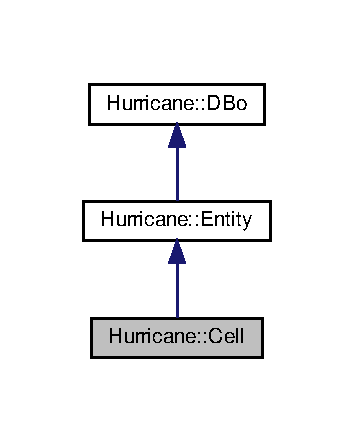
\includegraphics[width=178pt]{classHurricane_1_1Cell__inherit__graph}
\end{center}
\end{figure}
\subsection*{Public Member Functions}
\begin{DoxyCompactItemize}
\item 
\mbox{\hyperlink{classHurricane_1_1Library}{Library}} $\ast$ \mbox{\hyperlink{classHurricane_1_1Cell_aa84b97773160a28d3dd69df1e261eecf}{get\+Library}} () const
\item 
const \mbox{\hyperlink{classHurricane_1_1Name}{Name}} \& \mbox{\hyperlink{classHurricane_1_1Cell_a01cd4bba972d484496fd297648b8fa0c}{get\+Name}} () const
\item 
\mbox{\hyperlink{classHurricane_1_1Instance}{Instance}} $\ast$ \mbox{\hyperlink{classHurricane_1_1Cell_abaf178b24734de37cf0ac31918c096ac}{get\+Instance}} (const \mbox{\hyperlink{classHurricane_1_1Name}{Name}} \&name) const
\item 
\mbox{\hyperlink{namespaceHurricane_ac9436b03a2926f34ad6863deae2baadc}{Instances}} \mbox{\hyperlink{classHurricane_1_1Cell_aa85b3992431b672827167c5d9cb622f2}{get\+Instances}} () const
\item 
\mbox{\hyperlink{namespaceHurricane_ac9436b03a2926f34ad6863deae2baadc}{Instances}} \mbox{\hyperlink{classHurricane_1_1Cell_a3af933175d318b205d94adaf92ba0499}{get\+Instances\+Under}} (const \mbox{\hyperlink{classHurricane_1_1Box}{Box}} \&area, \mbox{\hyperlink{group__DbUGroup_ga4fbfa3e8c89347af76c9628ea06c4146}{Db\+U\+::\+Unit}} threshold=0) const
\item 
\mbox{\hyperlink{namespaceHurricane_ac9436b03a2926f34ad6863deae2baadc}{Instances}} \mbox{\hyperlink{classHurricane_1_1Cell_a7e51bee5db73dd44f788e591a5c175c8}{get\+Slave\+Instances}} () const
\item 
\mbox{\hyperlink{classHurricane_1_1Net}{Net}} $\ast$ \mbox{\hyperlink{classHurricane_1_1Cell_a63cb19881279b5af0a4e7dae707ef1bd}{get\+Net}} (const \mbox{\hyperlink{classHurricane_1_1Name}{Name}} \&name) const
\item 
\mbox{\hyperlink{namespaceHurricane_a3404a8b17130a1824f4a281704b04df7}{Nets}} \mbox{\hyperlink{classHurricane_1_1Cell_a8b4728abe83e9ec21d7bee1154218279}{get\+Nets}} () const
\item 
\mbox{\hyperlink{namespaceHurricane_a3404a8b17130a1824f4a281704b04df7}{Nets}} \mbox{\hyperlink{classHurricane_1_1Cell_a1512722d821edc18ff38e673862cd108}{get\+Global\+Nets}} () const
\item 
\mbox{\hyperlink{namespaceHurricane_a3404a8b17130a1824f4a281704b04df7}{Nets}} \mbox{\hyperlink{classHurricane_1_1Cell_aa80f3345db8c1395fa04a50737208793}{get\+External\+Nets}} () const
\item 
\mbox{\hyperlink{namespaceHurricane_a3404a8b17130a1824f4a281704b04df7}{Nets}} \mbox{\hyperlink{classHurricane_1_1Cell_a0da980d28ad60334da94a3966338f873}{get\+Internal\+Nets}} () const
\item 
\mbox{\hyperlink{namespaceHurricane_a3404a8b17130a1824f4a281704b04df7}{Nets}} \mbox{\hyperlink{classHurricane_1_1Cell_a306f28990f9fd4ccee0e9e8ebecf98fc}{get\+Clock\+Nets}} () const
\item 
\mbox{\hyperlink{namespaceHurricane_a3404a8b17130a1824f4a281704b04df7}{Nets}} \mbox{\hyperlink{classHurricane_1_1Cell_ac51c8f16de7a4af86feead9f1aecf494}{get\+Supply\+Nets}} () const
\item 
\mbox{\hyperlink{classHurricane_1_1Slice}{Slice}} $\ast$ \mbox{\hyperlink{classHurricane_1_1Cell_ac438b5b6b8dbcd868d6bf0deeb469444}{get\+Slice}} (const \mbox{\hyperlink{classHurricane_1_1Layer}{Layer}} $\ast$layer) const
\item 
\mbox{\hyperlink{namespaceHurricane_aa4a7e8a563c5687621eb5e57ade1706a}{Slices}} \mbox{\hyperlink{classHurricane_1_1Cell_aba933a81e3cacfc05b7bd1660e2a933a}{get\+Slices}} (const \mbox{\hyperlink{classHurricane_1_1Layer_af5277c670637bd5d910237e7afe01a91}{Layer\+::\+Mask}} \&mask=$\sim$0) const
\item 
\mbox{\hyperlink{namespaceHurricane_af8923abd57508cc44931a00d61b564ad}{Rubbers}} \mbox{\hyperlink{classHurricane_1_1Cell_a56395a189898d5ae2a869d5a5d5dfdbe}{get\+Rubbers}} () const
\item 
\mbox{\hyperlink{namespaceHurricane_af8923abd57508cc44931a00d61b564ad}{Rubbers}} \mbox{\hyperlink{classHurricane_1_1Cell_a58c6e24401d15f375547ad95b5c2c27c}{get\+Rubbers\+Under}} (const \mbox{\hyperlink{classHurricane_1_1Box}{Box}} \&area) const
\item 
\mbox{\hyperlink{namespaceHurricane_a7d26d99aeb5dd6d70d51bd35d2473e72}{Components}} \mbox{\hyperlink{classHurricane_1_1Cell_a14cb1b1f27e75d4af5b34a9a5956d818}{get\+Components}} (const \mbox{\hyperlink{classHurricane_1_1Layer_af5277c670637bd5d910237e7afe01a91}{Layer\+::\+Mask}} \&mask=$\sim$0) const
\item 
\mbox{\hyperlink{namespaceHurricane_a7d26d99aeb5dd6d70d51bd35d2473e72}{Components}} \mbox{\hyperlink{classHurricane_1_1Cell_a0a3c54d755ab36fe74bd032dfd43b53a}{get\+Components\+Under}} (const \mbox{\hyperlink{classHurricane_1_1Box}{Box}} \&area, const \mbox{\hyperlink{classHurricane_1_1Layer_af5277c670637bd5d910237e7afe01a91}{Layer\+::\+Mask}} \&mask=$\sim$0) const
\item 
\mbox{\hyperlink{namespaceHurricane_a1912927c128eee859af62dbe4cbe0a6b}{Occurrences}} \mbox{\hyperlink{classHurricane_1_1Cell_ab5bbab0a59106855d61deb94805e6115}{get\+Occurrences}} (unsigned search\+Depth=std\+::numeric\+\_\+limits$<$ unsigned int $>$\+::max()) const
\item 
\mbox{\hyperlink{namespaceHurricane_a1912927c128eee859af62dbe4cbe0a6b}{Occurrences}} \mbox{\hyperlink{classHurricane_1_1Cell_a7fb09c8e350923c47ce4c4407bdb00ce}{get\+Occurrences\+Under}} (const \mbox{\hyperlink{classHurricane_1_1Box}{Box}} \&area, unsigned search\+Depth=std\+::numeric\+\_\+limits$<$ unsigned int $>$\+::max()) const
\item 
\mbox{\hyperlink{namespaceHurricane_a1912927c128eee859af62dbe4cbe0a6b}{Occurrences}} \mbox{\hyperlink{classHurricane_1_1Cell_a30b71d9a35ff4e0b59b98ef515f26fc0}{get\+Terminal\+Instance\+Occurrences}} () const
\item 
\mbox{\hyperlink{namespaceHurricane_a1912927c128eee859af62dbe4cbe0a6b}{Occurrences}} \mbox{\hyperlink{classHurricane_1_1Cell_a6f559f7dab6e4afc0b60eba064c5e474}{get\+Terminal\+Netlist\+Instance\+Occurrences}} (const \mbox{\hyperlink{classHurricane_1_1Instance}{Instance}} $\ast$top\+Instance=N\+U\+LL) const
\item 
\mbox{\hyperlink{namespaceHurricane_a1912927c128eee859af62dbe4cbe0a6b}{Occurrences}} \mbox{\hyperlink{classHurricane_1_1Cell_a9e7a0536ec1efb23be2764068a85b6a7}{get\+Non\+Terminal\+Netlist\+Instance\+Occurrences}} (const \mbox{\hyperlink{classHurricane_1_1Instance}{Instance}} $\ast$top\+Instance=N\+U\+LL) const
\item 
const \mbox{\hyperlink{classHurricane_1_1Box}{Box}} \& \mbox{\hyperlink{classHurricane_1_1Cell_a142360ca7b3c1c637894f5b9a2cac069}{get\+Abutment\+Box}} () const
\item 
bool \mbox{\hyperlink{classHurricane_1_1Cell_a239354e1b4ad9b751abf5a064e43b0e6}{is\+Called\+By}} (\mbox{\hyperlink{classHurricane_1_1Cell}{Cell}} $\ast$cell) const
\item 
bool \mbox{\hyperlink{classHurricane_1_1Cell_aac4e9218b7806f3a0f2d5a55f00abd69}{is\+Terminal}} () const
\item 
bool \mbox{\hyperlink{classHurricane_1_1Cell_a6fe2b5a80d4b344733416b25ea559497}{is\+Terminal\+Netlist}} () const
\item 
bool \mbox{\hyperlink{classHurricane_1_1Cell_a6c2f2fd9f6f6e0578937a90c0c37a507}{is\+Unique}} () const
\item 
bool \mbox{\hyperlink{classHurricane_1_1Cell_a86c21867e9ce896eae72fd2999ce8a2d}{is\+Uniquified}} () const
\item 
bool \mbox{\hyperlink{classHurricane_1_1Cell_a0220dbbbe730e6874f7620135e9c10f6}{is\+Uniquify\+Master}} () const
\item 
void \mbox{\hyperlink{classHurricane_1_1Cell_ad2c9face922062664110c66ee205eab2}{set\+Name}} (const \mbox{\hyperlink{classHurricane_1_1Name}{Name}} \&name)
\item 
void \mbox{\hyperlink{classHurricane_1_1Cell_ab1949e2b708f0bd2d215ab90cfe864e0}{set\+Abutment\+Box}} (const \mbox{\hyperlink{classHurricane_1_1Box}{Box}} \&abutment\+Box)
\item 
void \mbox{\hyperlink{classHurricane_1_1Cell_a15958b25e911e8f5543557b6deea5618}{set\+Terminal\+Netlist}} (bool \mbox{\hyperlink{classHurricane_1_1Cell_a6fe2b5a80d4b344733416b25ea559497}{is\+Terminal\+Netlist}})
\item 
void \mbox{\hyperlink{classHurricane_1_1Cell_affefc597317063857f4904d4b16d5d4f}{materialize}} ()
\item 
void \mbox{\hyperlink{classHurricane_1_1Cell_a40c9ba4e3fc76b0c4bc58af8dcaddf53}{unmaterialize}} ()
\item 
\mbox{\hyperlink{classHurricane_1_1Cell}{Cell}} $\ast$ \mbox{\hyperlink{classHurricane_1_1Cell_a092f53c7f517ecc70d9ba375296c5d5b}{get\+Clone}} ()
\item 
void \mbox{\hyperlink{classHurricane_1_1Cell_aa113c121813342b6304f3e7fddbc8565}{uniquify}} (unsigned int depth=std\+::numeric\+\_\+limits$<$ unsigned int $>$\+::max())
\end{DoxyCompactItemize}
\subsection*{Static Public Member Functions}
\begin{DoxyCompactItemize}
\item 
static \mbox{\hyperlink{classHurricane_1_1Cell}{Cell}} $\ast$ \mbox{\hyperlink{classHurricane_1_1Cell_ad803afb3e52bea3bf3d520e353b162e0}{create}} (\mbox{\hyperlink{classHurricane_1_1Library}{Library}} $\ast$library, const \mbox{\hyperlink{classHurricane_1_1Name}{Name}} \&name)
\end{DoxyCompactItemize}


\subsection{Detailed Description}
The model ({\bfseries A\+PI}). 

\hypertarget{classHurricane_1_1Cell_secCellHierarchy}{}\subsection{Layout vs. Netlist Cell Hierarchy}\label{classHurricane_1_1Cell_secCellHierarchy}
The \mbox{\hyperlink{classHurricane_1_1Cell}{Cell}} / \mbox{\hyperlink{classHurricane_1_1Instance}{Instance}} hierarchy can be walkthrough in two different modes\+: 
\begin{DoxyItemize}
\item {\bfseries The Layout Mode}, in this mode the walktrough will be done over all the instances levels. This mode is used for the following collections\+: 
\begin{DoxyItemize}
\item \mbox{\hyperlink{classHurricane_1_1Cell_a30b71d9a35ff4e0b59b98ef515f26fc0}{Cell\+::get\+Terminal\+Instance\+Occurrences()}}. 
\end{DoxyItemize}


\item {\bfseries The Netlist Mode}, in this mode the walktrough will stop at instances flagged as Cell\+::\+Flags\+::\+Terminal\+Instance. The netlist hierarchy will be a subset of the layout one. Or, conversely, some level of layout hirearchy can have no netlist equivalent. This mode is used for the following collections\+:


\begin{DoxyItemize}
\item \mbox{\hyperlink{classHurricane_1_1Cell_a6f559f7dab6e4afc0b60eba064c5e474}{Cell\+::get\+Terminal\+Netlist\+Instance\+Occurrences()}}. 
\item \mbox{\hyperlink{classHurricane_1_1Cell_a9e7a0536ec1efb23be2764068a85b6a7}{Cell\+::get\+Non\+Terminal\+Netlist\+Instance\+Occurrences()}}. 
\end{DoxyItemize}
\end{DoxyItemize}

\subsection{Member Function Documentation}
\mbox{\Hypertarget{classHurricane_1_1Cell_ad803afb3e52bea3bf3d520e353b162e0}\label{classHurricane_1_1Cell_ad803afb3e52bea3bf3d520e353b162e0}} 
\index{Hurricane\+::\+Cell@{Hurricane\+::\+Cell}!create@{create}}
\index{create@{create}!Hurricane\+::\+Cell@{Hurricane\+::\+Cell}}
\subsubsection{\texorpdfstring{create()}{create()}}
{\footnotesize\ttfamily \mbox{\hyperlink{classHurricane_1_1Cell}{Cell}} $\ast$ Hurricane\+::\+Cell\+::create (\begin{DoxyParamCaption}\item[{\mbox{\hyperlink{classHurricane_1_1Library}{Library}} $\ast$}]{library,  }\item[{const \mbox{\hyperlink{classHurricane_1_1Name}{Name}} \&}]{name }\end{DoxyParamCaption})\hspace{0.3cm}{\ttfamily [static]}}

creates and returns a new \mbox{\hyperlink{classHurricane_1_1Cell}{Cell}} named {\itshape name} for the \mbox{\hyperlink{classHurricane_1_1Library}{Library}} {\itshape library}.

\begin{DoxyParagraph}{Caution\+: Throws an exception if the Library is null, if the Name is}
empty or if a cell with same name already exists in the \mbox{\hyperlink{classHurricane_1_1Library}{Library}}. 
\end{DoxyParagraph}
\mbox{\Hypertarget{classHurricane_1_1Cell_aa84b97773160a28d3dd69df1e261eecf}\label{classHurricane_1_1Cell_aa84b97773160a28d3dd69df1e261eecf}} 
\index{Hurricane\+::\+Cell@{Hurricane\+::\+Cell}!get\+Library@{get\+Library}}
\index{get\+Library@{get\+Library}!Hurricane\+::\+Cell@{Hurricane\+::\+Cell}}
\subsubsection{\texorpdfstring{get\+Library()}{getLibrary()}}
{\footnotesize\ttfamily \mbox{\hyperlink{classHurricane_1_1Library}{Library}} $\ast$ Hurricane\+::\+Cell\+::get\+Library (\begin{DoxyParamCaption}{ }\end{DoxyParamCaption}) const\hspace{0.3cm}{\ttfamily [inline]}}

Returns the \mbox{\hyperlink{classHurricane_1_1Library}{Library}} owning the \mbox{\hyperlink{classHurricane_1_1Cell}{Cell}}. \mbox{\Hypertarget{classHurricane_1_1Cell_a01cd4bba972d484496fd297648b8fa0c}\label{classHurricane_1_1Cell_a01cd4bba972d484496fd297648b8fa0c}} 
\index{Hurricane\+::\+Cell@{Hurricane\+::\+Cell}!get\+Name@{get\+Name}}
\index{get\+Name@{get\+Name}!Hurricane\+::\+Cell@{Hurricane\+::\+Cell}}
\subsubsection{\texorpdfstring{get\+Name()}{getName()}}
{\footnotesize\ttfamily const \mbox{\hyperlink{classHurricane_1_1Name}{Name}} \& Hurricane\+::\+Cell\+::get\+Name (\begin{DoxyParamCaption}{ }\end{DoxyParamCaption}) const\hspace{0.3cm}{\ttfamily [inline]}}

Returns the \mbox{\hyperlink{classHurricane_1_1Name}{Name}} of the \mbox{\hyperlink{classHurricane_1_1Cell}{Cell}}. \mbox{\Hypertarget{classHurricane_1_1Cell_abaf178b24734de37cf0ac31918c096ac}\label{classHurricane_1_1Cell_abaf178b24734de37cf0ac31918c096ac}} 
\index{Hurricane\+::\+Cell@{Hurricane\+::\+Cell}!get\+Instance@{get\+Instance}}
\index{get\+Instance@{get\+Instance}!Hurricane\+::\+Cell@{Hurricane\+::\+Cell}}
\subsubsection{\texorpdfstring{get\+Instance()}{getInstance()}}
{\footnotesize\ttfamily \mbox{\hyperlink{classHurricane_1_1Instance}{Instance}} $\ast$ Hurricane\+::\+Cell\+::get\+Instance (\begin{DoxyParamCaption}\item[{const \mbox{\hyperlink{classHurricane_1_1Name}{Name}} \&}]{name }\end{DoxyParamCaption}) const\hspace{0.3cm}{\ttfamily [inline]}}

Returns the \mbox{\hyperlink{classHurricane_1_1Instance}{Instance}} of name {\itshape name} if it exists, else {\ttfamily N\+U\+LL}. \mbox{\Hypertarget{classHurricane_1_1Cell_aa85b3992431b672827167c5d9cb622f2}\label{classHurricane_1_1Cell_aa85b3992431b672827167c5d9cb622f2}} 
\index{Hurricane\+::\+Cell@{Hurricane\+::\+Cell}!get\+Instances@{get\+Instances}}
\index{get\+Instances@{get\+Instances}!Hurricane\+::\+Cell@{Hurricane\+::\+Cell}}
\subsubsection{\texorpdfstring{get\+Instances()}{getInstances()}}
{\footnotesize\ttfamily \mbox{\hyperlink{namespaceHurricane_ac9436b03a2926f34ad6863deae2baadc}{Instances}} Hurricane\+::\+Cell\+::get\+Instances (\begin{DoxyParamCaption}{ }\end{DoxyParamCaption}) const\hspace{0.3cm}{\ttfamily [inline]}}

Returns the \mbox{\hyperlink{classHurricane_1_1Collection}{Collection}} of all instances called by the \mbox{\hyperlink{classHurricane_1_1Cell}{Cell}}. \mbox{\Hypertarget{classHurricane_1_1Cell_a3af933175d318b205d94adaf92ba0499}\label{classHurricane_1_1Cell_a3af933175d318b205d94adaf92ba0499}} 
\index{Hurricane\+::\+Cell@{Hurricane\+::\+Cell}!get\+Instances\+Under@{get\+Instances\+Under}}
\index{get\+Instances\+Under@{get\+Instances\+Under}!Hurricane\+::\+Cell@{Hurricane\+::\+Cell}}
\subsubsection{\texorpdfstring{get\+Instances\+Under()}{getInstancesUnder()}}
{\footnotesize\ttfamily \mbox{\hyperlink{namespaceHurricane_ac9436b03a2926f34ad6863deae2baadc}{Instances}} Hurricane\+::\+Cell\+::get\+Instances\+Under (\begin{DoxyParamCaption}\item[{const \mbox{\hyperlink{classHurricane_1_1Box}{Box}} \&}]{area,  }\item[{\mbox{\hyperlink{group__DbUGroup_ga4fbfa3e8c89347af76c9628ea06c4146}{Db\+U\+::\+Unit}}}]{threshold = {\ttfamily 0} }\end{DoxyParamCaption}) const}

Returns the collection of all instances of the \mbox{\hyperlink{classHurricane_1_1Cell}{Cell}} intersecting the given rectangular {\itshape area}. \mbox{\Hypertarget{classHurricane_1_1Cell_a7e51bee5db73dd44f788e591a5c175c8}\label{classHurricane_1_1Cell_a7e51bee5db73dd44f788e591a5c175c8}} 
\index{Hurricane\+::\+Cell@{Hurricane\+::\+Cell}!get\+Slave\+Instances@{get\+Slave\+Instances}}
\index{get\+Slave\+Instances@{get\+Slave\+Instances}!Hurricane\+::\+Cell@{Hurricane\+::\+Cell}}
\subsubsection{\texorpdfstring{get\+Slave\+Instances()}{getSlaveInstances()}}
{\footnotesize\ttfamily \mbox{\hyperlink{namespaceHurricane_ac9436b03a2926f34ad6863deae2baadc}{Instances}} Hurricane\+::\+Cell\+::get\+Slave\+Instances (\begin{DoxyParamCaption}{ }\end{DoxyParamCaption}) const}

Returns the \mbox{\hyperlink{classHurricane_1_1Collection}{Collection}} of instances whose master is this \mbox{\hyperlink{classHurricane_1_1Cell}{Cell}}. \mbox{\Hypertarget{classHurricane_1_1Cell_a63cb19881279b5af0a4e7dae707ef1bd}\label{classHurricane_1_1Cell_a63cb19881279b5af0a4e7dae707ef1bd}} 
\index{Hurricane\+::\+Cell@{Hurricane\+::\+Cell}!get\+Net@{get\+Net}}
\index{get\+Net@{get\+Net}!Hurricane\+::\+Cell@{Hurricane\+::\+Cell}}
\subsubsection{\texorpdfstring{get\+Net()}{getNet()}}
{\footnotesize\ttfamily \mbox{\hyperlink{classHurricane_1_1Net}{Net}} $\ast$ Hurricane\+::\+Cell\+::get\+Net (\begin{DoxyParamCaption}\item[{const \mbox{\hyperlink{classHurricane_1_1Name}{Name}} \&}]{name }\end{DoxyParamCaption}) const}

Returns the \mbox{\hyperlink{classHurricane_1_1Net}{Net}} of name {\itshape name} if it exists, else {\ttfamily N\+U\+LL}. \mbox{\Hypertarget{classHurricane_1_1Cell_a8b4728abe83e9ec21d7bee1154218279}\label{classHurricane_1_1Cell_a8b4728abe83e9ec21d7bee1154218279}} 
\index{Hurricane\+::\+Cell@{Hurricane\+::\+Cell}!get\+Nets@{get\+Nets}}
\index{get\+Nets@{get\+Nets}!Hurricane\+::\+Cell@{Hurricane\+::\+Cell}}
\subsubsection{\texorpdfstring{get\+Nets()}{getNets()}}
{\footnotesize\ttfamily \mbox{\hyperlink{namespaceHurricane_a3404a8b17130a1824f4a281704b04df7}{Nets}} Hurricane\+::\+Cell\+::get\+Nets (\begin{DoxyParamCaption}{ }\end{DoxyParamCaption}) const\hspace{0.3cm}{\ttfamily [inline]}}

Returns the \mbox{\hyperlink{classHurricane_1_1Collection}{Collection}} of all nets of the \mbox{\hyperlink{classHurricane_1_1Cell}{Cell}}. \mbox{\Hypertarget{classHurricane_1_1Cell_a1512722d821edc18ff38e673862cd108}\label{classHurricane_1_1Cell_a1512722d821edc18ff38e673862cd108}} 
\index{Hurricane\+::\+Cell@{Hurricane\+::\+Cell}!get\+Global\+Nets@{get\+Global\+Nets}}
\index{get\+Global\+Nets@{get\+Global\+Nets}!Hurricane\+::\+Cell@{Hurricane\+::\+Cell}}
\subsubsection{\texorpdfstring{get\+Global\+Nets()}{getGlobalNets()}}
{\footnotesize\ttfamily \mbox{\hyperlink{namespaceHurricane_a3404a8b17130a1824f4a281704b04df7}{Nets}} Hurricane\+::\+Cell\+::get\+Global\+Nets (\begin{DoxyParamCaption}{ }\end{DoxyParamCaption}) const}

Returns the \mbox{\hyperlink{classHurricane_1_1Collection}{Collection}} of all global nets of the \mbox{\hyperlink{classHurricane_1_1Cell}{Cell}}. \mbox{\Hypertarget{classHurricane_1_1Cell_aa80f3345db8c1395fa04a50737208793}\label{classHurricane_1_1Cell_aa80f3345db8c1395fa04a50737208793}} 
\index{Hurricane\+::\+Cell@{Hurricane\+::\+Cell}!get\+External\+Nets@{get\+External\+Nets}}
\index{get\+External\+Nets@{get\+External\+Nets}!Hurricane\+::\+Cell@{Hurricane\+::\+Cell}}
\subsubsection{\texorpdfstring{get\+External\+Nets()}{getExternalNets()}}
{\footnotesize\ttfamily \mbox{\hyperlink{namespaceHurricane_a3404a8b17130a1824f4a281704b04df7}{Nets}} Hurricane\+::\+Cell\+::get\+External\+Nets (\begin{DoxyParamCaption}{ }\end{DoxyParamCaption}) const}

Returns the \mbox{\hyperlink{classHurricane_1_1Collection}{Collection}} of all external nets of the \mbox{\hyperlink{classHurricane_1_1Cell}{Cell}}. \mbox{\Hypertarget{classHurricane_1_1Cell_a0da980d28ad60334da94a3966338f873}\label{classHurricane_1_1Cell_a0da980d28ad60334da94a3966338f873}} 
\index{Hurricane\+::\+Cell@{Hurricane\+::\+Cell}!get\+Internal\+Nets@{get\+Internal\+Nets}}
\index{get\+Internal\+Nets@{get\+Internal\+Nets}!Hurricane\+::\+Cell@{Hurricane\+::\+Cell}}
\subsubsection{\texorpdfstring{get\+Internal\+Nets()}{getInternalNets()}}
{\footnotesize\ttfamily \mbox{\hyperlink{namespaceHurricane_a3404a8b17130a1824f4a281704b04df7}{Nets}} Hurricane\+::\+Cell\+::get\+Internal\+Nets (\begin{DoxyParamCaption}{ }\end{DoxyParamCaption}) const}

Returns the \mbox{\hyperlink{classHurricane_1_1Collection}{Collection}} of all internal nets of the \mbox{\hyperlink{classHurricane_1_1Cell}{Cell}}. \mbox{\Hypertarget{classHurricane_1_1Cell_a306f28990f9fd4ccee0e9e8ebecf98fc}\label{classHurricane_1_1Cell_a306f28990f9fd4ccee0e9e8ebecf98fc}} 
\index{Hurricane\+::\+Cell@{Hurricane\+::\+Cell}!get\+Clock\+Nets@{get\+Clock\+Nets}}
\index{get\+Clock\+Nets@{get\+Clock\+Nets}!Hurricane\+::\+Cell@{Hurricane\+::\+Cell}}
\subsubsection{\texorpdfstring{get\+Clock\+Nets()}{getClockNets()}}
{\footnotesize\ttfamily \mbox{\hyperlink{namespaceHurricane_a3404a8b17130a1824f4a281704b04df7}{Nets}} Hurricane\+::\+Cell\+::get\+Clock\+Nets (\begin{DoxyParamCaption}{ }\end{DoxyParamCaption}) const}

Returns the \mbox{\hyperlink{classHurricane_1_1Collection}{Collection}} of all clock nets of the \mbox{\hyperlink{classHurricane_1_1Cell}{Cell}}. \mbox{\Hypertarget{classHurricane_1_1Cell_ac51c8f16de7a4af86feead9f1aecf494}\label{classHurricane_1_1Cell_ac51c8f16de7a4af86feead9f1aecf494}} 
\index{Hurricane\+::\+Cell@{Hurricane\+::\+Cell}!get\+Supply\+Nets@{get\+Supply\+Nets}}
\index{get\+Supply\+Nets@{get\+Supply\+Nets}!Hurricane\+::\+Cell@{Hurricane\+::\+Cell}}
\subsubsection{\texorpdfstring{get\+Supply\+Nets()}{getSupplyNets()}}
{\footnotesize\ttfamily \mbox{\hyperlink{namespaceHurricane_a3404a8b17130a1824f4a281704b04df7}{Nets}} Hurricane\+::\+Cell\+::get\+Supply\+Nets (\begin{DoxyParamCaption}{ }\end{DoxyParamCaption}) const}

Returns the \mbox{\hyperlink{classHurricane_1_1Collection}{Collection}} of all supply nets of the \mbox{\hyperlink{classHurricane_1_1Cell}{Cell}}. \mbox{\Hypertarget{classHurricane_1_1Cell_ac438b5b6b8dbcd868d6bf0deeb469444}\label{classHurricane_1_1Cell_ac438b5b6b8dbcd868d6bf0deeb469444}} 
\index{Hurricane\+::\+Cell@{Hurricane\+::\+Cell}!get\+Slice@{get\+Slice}}
\index{get\+Slice@{get\+Slice}!Hurricane\+::\+Cell@{Hurricane\+::\+Cell}}
\subsubsection{\texorpdfstring{get\+Slice()}{getSlice()}}
{\footnotesize\ttfamily \mbox{\hyperlink{classHurricane_1_1Slice}{Slice}} $\ast$ Hurricane\+::\+Cell\+::get\+Slice (\begin{DoxyParamCaption}\item[{const \mbox{\hyperlink{classHurricane_1_1Layer}{Layer}} $\ast$}]{layer }\end{DoxyParamCaption}) const\hspace{0.3cm}{\ttfamily [inline]}}

Returns the \mbox{\hyperlink{classHurricane_1_1Slice}{Slice}} associated with the \mbox{\hyperlink{classHurricane_1_1Layer}{Layer}} {\itshape layer} if it exists, else {\ttfamily N\+U\+LL}. \mbox{\Hypertarget{classHurricane_1_1Cell_aba933a81e3cacfc05b7bd1660e2a933a}\label{classHurricane_1_1Cell_aba933a81e3cacfc05b7bd1660e2a933a}} 
\index{Hurricane\+::\+Cell@{Hurricane\+::\+Cell}!get\+Slices@{get\+Slices}}
\index{get\+Slices@{get\+Slices}!Hurricane\+::\+Cell@{Hurricane\+::\+Cell}}
\subsubsection{\texorpdfstring{get\+Slices()}{getSlices()}}
{\footnotesize\ttfamily \mbox{\hyperlink{namespaceHurricane_aa4a7e8a563c5687621eb5e57ade1706a}{Slices}} Hurricane\+::\+Cell\+::get\+Slices (\begin{DoxyParamCaption}\item[{const \mbox{\hyperlink{classHurricane_1_1Layer_af5277c670637bd5d910237e7afe01a91}{Layer\+::\+Mask}} \&}]{mask = {\ttfamily $\sim$0} }\end{DoxyParamCaption}) const}

Returns the \mbox{\hyperlink{classHurricane_1_1Collection}{Collection}} of slices of a \mbox{\hyperlink{classHurricane_1_1Cell}{Cell}}. \mbox{\Hypertarget{classHurricane_1_1Cell_a56395a189898d5ae2a869d5a5d5dfdbe}\label{classHurricane_1_1Cell_a56395a189898d5ae2a869d5a5d5dfdbe}} 
\index{Hurricane\+::\+Cell@{Hurricane\+::\+Cell}!get\+Rubbers@{get\+Rubbers}}
\index{get\+Rubbers@{get\+Rubbers}!Hurricane\+::\+Cell@{Hurricane\+::\+Cell}}
\subsubsection{\texorpdfstring{get\+Rubbers()}{getRubbers()}}
{\footnotesize\ttfamily \mbox{\hyperlink{namespaceHurricane_af8923abd57508cc44931a00d61b564ad}{Rubbers}} Hurricane\+::\+Cell\+::get\+Rubbers (\begin{DoxyParamCaption}{ }\end{DoxyParamCaption}) const}

Returns the \mbox{\hyperlink{classHurricane_1_1Collection}{Collection}} of all Rubbers of a \mbox{\hyperlink{classHurricane_1_1Cell}{Cell}}. \mbox{\Hypertarget{classHurricane_1_1Cell_a58c6e24401d15f375547ad95b5c2c27c}\label{classHurricane_1_1Cell_a58c6e24401d15f375547ad95b5c2c27c}} 
\index{Hurricane\+::\+Cell@{Hurricane\+::\+Cell}!get\+Rubbers\+Under@{get\+Rubbers\+Under}}
\index{get\+Rubbers\+Under@{get\+Rubbers\+Under}!Hurricane\+::\+Cell@{Hurricane\+::\+Cell}}
\subsubsection{\texorpdfstring{get\+Rubbers\+Under()}{getRubbersUnder()}}
{\footnotesize\ttfamily \mbox{\hyperlink{namespaceHurricane_af8923abd57508cc44931a00d61b564ad}{Rubbers}} Hurricane\+::\+Cell\+::get\+Rubbers\+Under (\begin{DoxyParamCaption}\item[{const \mbox{\hyperlink{classHurricane_1_1Box}{Box}} \&}]{area }\end{DoxyParamCaption}) const}

Returns the collection of all Rubbers of the \mbox{\hyperlink{classHurricane_1_1Cell}{Cell}} intersecting the given rectangular {\itshape area}.

\begin{DoxyParagraph}{Caution\+: Only currently materialized rubbers are taken into account}
in this collection. 
\end{DoxyParagraph}
\mbox{\Hypertarget{classHurricane_1_1Cell_a14cb1b1f27e75d4af5b34a9a5956d818}\label{classHurricane_1_1Cell_a14cb1b1f27e75d4af5b34a9a5956d818}} 
\index{Hurricane\+::\+Cell@{Hurricane\+::\+Cell}!get\+Components@{get\+Components}}
\index{get\+Components@{get\+Components}!Hurricane\+::\+Cell@{Hurricane\+::\+Cell}}
\subsubsection{\texorpdfstring{get\+Components()}{getComponents()}}
{\footnotesize\ttfamily \mbox{\hyperlink{namespaceHurricane_a7d26d99aeb5dd6d70d51bd35d2473e72}{Components}} Hurricane\+::\+Cell\+::get\+Components (\begin{DoxyParamCaption}\item[{const \mbox{\hyperlink{classHurricane_1_1Layer_af5277c670637bd5d910237e7afe01a91}{Layer\+::\+Mask}} \&}]{mask = {\ttfamily $\sim$0} }\end{DoxyParamCaption}) const}

Returns the \mbox{\hyperlink{classHurricane_1_1Collection}{Collection}} of all Components of the \mbox{\hyperlink{classHurricane_1_1Cell}{Cell}}. \mbox{\Hypertarget{classHurricane_1_1Cell_a0a3c54d755ab36fe74bd032dfd43b53a}\label{classHurricane_1_1Cell_a0a3c54d755ab36fe74bd032dfd43b53a}} 
\index{Hurricane\+::\+Cell@{Hurricane\+::\+Cell}!get\+Components\+Under@{get\+Components\+Under}}
\index{get\+Components\+Under@{get\+Components\+Under}!Hurricane\+::\+Cell@{Hurricane\+::\+Cell}}
\subsubsection{\texorpdfstring{get\+Components\+Under()}{getComponentsUnder()}}
{\footnotesize\ttfamily \mbox{\hyperlink{namespaceHurricane_a7d26d99aeb5dd6d70d51bd35d2473e72}{Components}} Hurricane\+::\+Cell\+::get\+Components\+Under (\begin{DoxyParamCaption}\item[{const \mbox{\hyperlink{classHurricane_1_1Box}{Box}} \&}]{area,  }\item[{const \mbox{\hyperlink{classHurricane_1_1Layer_af5277c670637bd5d910237e7afe01a91}{Layer\+::\+Mask}} \&}]{mask = {\ttfamily $\sim$0} }\end{DoxyParamCaption}) const}

Returns the collection of all Components of the \mbox{\hyperlink{classHurricane_1_1Cell}{Cell}} intersecting the given rectangular {\itshape area}.

\begin{DoxyParagraph}{Caution\+: Only currently materialized Components are taken into account}
in this collection. 
\end{DoxyParagraph}
\mbox{\Hypertarget{classHurricane_1_1Cell_ab5bbab0a59106855d61deb94805e6115}\label{classHurricane_1_1Cell_ab5bbab0a59106855d61deb94805e6115}} 
\index{Hurricane\+::\+Cell@{Hurricane\+::\+Cell}!get\+Occurrences@{get\+Occurrences}}
\index{get\+Occurrences@{get\+Occurrences}!Hurricane\+::\+Cell@{Hurricane\+::\+Cell}}
\subsubsection{\texorpdfstring{get\+Occurrences()}{getOccurrences()}}
{\footnotesize\ttfamily \mbox{\hyperlink{namespaceHurricane_a1912927c128eee859af62dbe4cbe0a6b}{Occurrences}} Hurricane\+::\+Cell\+::get\+Occurrences (\begin{DoxyParamCaption}\item[{unsigned}]{search\+Depth = {\ttfamily std\+:\+:numeric\+\_\+limits$<$unsigned~int$>$\+:\+:max()} }\end{DoxyParamCaption}) const}

Returns the \mbox{\hyperlink{classHurricane_1_1Collection}{Collection}} of all Occurrences belonging to this \mbox{\hyperlink{classHurricane_1_1Cell}{Cell}}.

\begin{DoxyRemark}{Remarks}
The search depth is decremented each time a hirearchical level is crossed. The search ends when depth becomes null (the value {\ttfamily I\+N\+F\+I\+N\+I\+TE} is equal to {\ttfamily }(unsigned)-\/1) . 
\end{DoxyRemark}
\mbox{\Hypertarget{classHurricane_1_1Cell_a7fb09c8e350923c47ce4c4407bdb00ce}\label{classHurricane_1_1Cell_a7fb09c8e350923c47ce4c4407bdb00ce}} 
\index{Hurricane\+::\+Cell@{Hurricane\+::\+Cell}!get\+Occurrences\+Under@{get\+Occurrences\+Under}}
\index{get\+Occurrences\+Under@{get\+Occurrences\+Under}!Hurricane\+::\+Cell@{Hurricane\+::\+Cell}}
\subsubsection{\texorpdfstring{get\+Occurrences\+Under()}{getOccurrencesUnder()}}
{\footnotesize\ttfamily \mbox{\hyperlink{namespaceHurricane_a1912927c128eee859af62dbe4cbe0a6b}{Occurrences}} Hurricane\+::\+Cell\+::get\+Occurrences\+Under (\begin{DoxyParamCaption}\item[{const \mbox{\hyperlink{classHurricane_1_1Box}{Box}} \&}]{area,  }\item[{unsigned}]{search\+Depth = {\ttfamily std\+:\+:numeric\+\_\+limits$<$unsigned~int$>$\+:\+:max()} }\end{DoxyParamCaption}) const}

Returns the \mbox{\hyperlink{classHurricane_1_1Collection}{Collection}} of all Occurrences belonging to this \mbox{\hyperlink{classHurricane_1_1Cell}{Cell}} and intersecting the given rectangular area.

\begin{DoxyRemark}{Remarks}
The search depth is decremented each time a hirearchical level is crossed. The search ends when depth becomes null (the value {\ttfamily I\+N\+F\+I\+N\+I\+TE} is equal to {\ttfamily }(unsigned)-\/1) .
\end{DoxyRemark}
\begin{DoxyParagraph}{Caution\+: Only occurences corresponding to currently materialized}
entities are taken into account in this \mbox{\hyperlink{classHurricane_1_1Collection}{Collection}}. 
\end{DoxyParagraph}
\mbox{\Hypertarget{classHurricane_1_1Cell_a30b71d9a35ff4e0b59b98ef515f26fc0}\label{classHurricane_1_1Cell_a30b71d9a35ff4e0b59b98ef515f26fc0}} 
\index{Hurricane\+::\+Cell@{Hurricane\+::\+Cell}!get\+Terminal\+Instance\+Occurrences@{get\+Terminal\+Instance\+Occurrences}}
\index{get\+Terminal\+Instance\+Occurrences@{get\+Terminal\+Instance\+Occurrences}!Hurricane\+::\+Cell@{Hurricane\+::\+Cell}}
\subsubsection{\texorpdfstring{get\+Terminal\+Instance\+Occurrences()}{getTerminalInstanceOccurrences()}}
{\footnotesize\ttfamily \mbox{\hyperlink{namespaceHurricane_a1912927c128eee859af62dbe4cbe0a6b}{Occurrences}} Hurricane\+::\+Cell\+::get\+Terminal\+Instance\+Occurrences (\begin{DoxyParamCaption}{ }\end{DoxyParamCaption}) const}

Returns the trans-\/hierarchical \mbox{\hyperlink{classHurricane_1_1Collection}{Collection}} of all instance Occurrences that are layout terminal cells (leaves). \mbox{\Hypertarget{classHurricane_1_1Cell_a6f559f7dab6e4afc0b60eba064c5e474}\label{classHurricane_1_1Cell_a6f559f7dab6e4afc0b60eba064c5e474}} 
\index{Hurricane\+::\+Cell@{Hurricane\+::\+Cell}!get\+Terminal\+Netlist\+Instance\+Occurrences@{get\+Terminal\+Netlist\+Instance\+Occurrences}}
\index{get\+Terminal\+Netlist\+Instance\+Occurrences@{get\+Terminal\+Netlist\+Instance\+Occurrences}!Hurricane\+::\+Cell@{Hurricane\+::\+Cell}}
\subsubsection{\texorpdfstring{get\+Terminal\+Netlist\+Instance\+Occurrences()}{getTerminalNetlistInstanceOccurrences()}}
{\footnotesize\ttfamily \mbox{\hyperlink{namespaceHurricane_a1912927c128eee859af62dbe4cbe0a6b}{Occurrences}} Hurricane\+::\+Cell\+::get\+Terminal\+Netlist\+Instance\+Occurrences (\begin{DoxyParamCaption}\item[{const \mbox{\hyperlink{classHurricane_1_1Instance}{Instance}} $\ast$}]{top\+Instance = {\ttfamily NULL} }\end{DoxyParamCaption}) const}

Returns the trans-\/hierarchical \mbox{\hyperlink{classHurricane_1_1Collection}{Collection}} of all instance Occurrences that are leaf cells. With the {\ttfamily top\+Instance} argument we can restrict the collection to leafs of that instance (of the current \mbox{\hyperlink{classHurricane_1_1Cell}{Cell}}) only. \mbox{\Hypertarget{classHurricane_1_1Cell_a9e7a0536ec1efb23be2764068a85b6a7}\label{classHurricane_1_1Cell_a9e7a0536ec1efb23be2764068a85b6a7}} 
\index{Hurricane\+::\+Cell@{Hurricane\+::\+Cell}!get\+Non\+Terminal\+Netlist\+Instance\+Occurrences@{get\+Non\+Terminal\+Netlist\+Instance\+Occurrences}}
\index{get\+Non\+Terminal\+Netlist\+Instance\+Occurrences@{get\+Non\+Terminal\+Netlist\+Instance\+Occurrences}!Hurricane\+::\+Cell@{Hurricane\+::\+Cell}}
\subsubsection{\texorpdfstring{get\+Non\+Terminal\+Netlist\+Instance\+Occurrences()}{getNonTerminalNetlistInstanceOccurrences()}}
{\footnotesize\ttfamily \mbox{\hyperlink{namespaceHurricane_a1912927c128eee859af62dbe4cbe0a6b}{Occurrences}} Hurricane\+::\+Cell\+::get\+Non\+Terminal\+Netlist\+Instance\+Occurrences (\begin{DoxyParamCaption}\item[{const \mbox{\hyperlink{classHurricane_1_1Instance}{Instance}} $\ast$}]{top\+Instance = {\ttfamily NULL} }\end{DoxyParamCaption}) const}

Returns the trans-\/hierarchical \mbox{\hyperlink{classHurricane_1_1Collection}{Collection}} of all instance Occurrences that are {\bfseries not} leaf cells. With the {\ttfamily top\+Instance} argument we can restrict the collection to non-\/leafs of that instance (of the current \mbox{\hyperlink{classHurricane_1_1Cell}{Cell}}) only. \mbox{\Hypertarget{classHurricane_1_1Cell_a142360ca7b3c1c637894f5b9a2cac069}\label{classHurricane_1_1Cell_a142360ca7b3c1c637894f5b9a2cac069}} 
\index{Hurricane\+::\+Cell@{Hurricane\+::\+Cell}!get\+Abutment\+Box@{get\+Abutment\+Box}}
\index{get\+Abutment\+Box@{get\+Abutment\+Box}!Hurricane\+::\+Cell@{Hurricane\+::\+Cell}}
\subsubsection{\texorpdfstring{get\+Abutment\+Box()}{getAbutmentBox()}}
{\footnotesize\ttfamily \mbox{\hyperlink{classHurricane_1_1Box}{Box}} Hurricane\+::\+Cell\+::get\+Abutment\+Box (\begin{DoxyParamCaption}{ }\end{DoxyParamCaption}) const\hspace{0.3cm}{\ttfamily [inline]}}

Returns Returns the abutment box of the cell (which is defined by the designer unlike the bounding box which is managed dynamically). \mbox{\Hypertarget{classHurricane_1_1Cell_a239354e1b4ad9b751abf5a064e43b0e6}\label{classHurricane_1_1Cell_a239354e1b4ad9b751abf5a064e43b0e6}} 
\index{Hurricane\+::\+Cell@{Hurricane\+::\+Cell}!is\+Called\+By@{is\+Called\+By}}
\index{is\+Called\+By@{is\+Called\+By}!Hurricane\+::\+Cell@{Hurricane\+::\+Cell}}
\subsubsection{\texorpdfstring{is\+Called\+By()}{isCalledBy()}}
{\footnotesize\ttfamily bool Hurricane\+::\+Cell\+::is\+Called\+By (\begin{DoxyParamCaption}\item[{\mbox{\hyperlink{classHurricane_1_1Cell}{Cell}} $\ast$}]{cell }\end{DoxyParamCaption}) const}

Returns {\bfseries true} if the cell {\ttfamily this} is directly or indirectly called by the \mbox{\hyperlink{classHurricane_1_1Cell}{Cell}} {\itshape cell}. This functions allows to check that there is no cyclic instance calls of cells (it is by default, automatically called when creating an instance). \mbox{\Hypertarget{classHurricane_1_1Cell_aac4e9218b7806f3a0f2d5a55f00abd69}\label{classHurricane_1_1Cell_aac4e9218b7806f3a0f2d5a55f00abd69}} 
\index{Hurricane\+::\+Cell@{Hurricane\+::\+Cell}!is\+Terminal@{is\+Terminal}}
\index{is\+Terminal@{is\+Terminal}!Hurricane\+::\+Cell@{Hurricane\+::\+Cell}}
\subsubsection{\texorpdfstring{is\+Terminal()}{isTerminal()}}
{\footnotesize\ttfamily bool Hurricane\+::\+Cell\+::is\+Terminal (\begin{DoxyParamCaption}{ }\end{DoxyParamCaption}) const\hspace{0.3cm}{\ttfamily [inline]}}

Returns {\bfseries true} if the cell contains no instances. This is a layout leaf cell. \mbox{\Hypertarget{classHurricane_1_1Cell_a6fe2b5a80d4b344733416b25ea559497}\label{classHurricane_1_1Cell_a6fe2b5a80d4b344733416b25ea559497}} 
\index{Hurricane\+::\+Cell@{Hurricane\+::\+Cell}!is\+Terminal\+Netlist@{is\+Terminal\+Netlist}}
\index{is\+Terminal\+Netlist@{is\+Terminal\+Netlist}!Hurricane\+::\+Cell@{Hurricane\+::\+Cell}}
\subsubsection{\texorpdfstring{is\+Terminal\+Netlist()}{isTerminalNetlist()}}
{\footnotesize\ttfamily bool Hurricane\+::\+Cell\+::is\+Terminal\+Netlist (\begin{DoxyParamCaption}{ }\end{DoxyParamCaption}) const\hspace{0.3cm}{\ttfamily [inline]}}

Returns {\bfseries true} if the \mbox{\hyperlink{classHurricane_1_1Cell}{Cell}} is marked as terminal for the {\itshape netlist} hierarchy. A terminal {\itshape netlist} cell may, however contains further level of physical (layout) instances. This is a state that can be set or unset. 

Referenced by set\+Terminal\+Netlist().

\mbox{\Hypertarget{classHurricane_1_1Cell_a6c2f2fd9f6f6e0578937a90c0c37a507}\label{classHurricane_1_1Cell_a6c2f2fd9f6f6e0578937a90c0c37a507}} 
\index{Hurricane\+::\+Cell@{Hurricane\+::\+Cell}!is\+Unique@{is\+Unique}}
\index{is\+Unique@{is\+Unique}!Hurricane\+::\+Cell@{Hurricane\+::\+Cell}}
\subsubsection{\texorpdfstring{is\+Unique()}{isUnique()}}
{\footnotesize\ttfamily bool Hurricane\+::\+Cell\+::is\+Unique (\begin{DoxyParamCaption}{ }\end{DoxyParamCaption}) const}

Returns {\bfseries true} if the \mbox{\hyperlink{classHurricane_1_1Cell}{Cell}} has one or less instances, regardless of it\textquotesingle{}s uniquification state. \mbox{\Hypertarget{classHurricane_1_1Cell_a86c21867e9ce896eae72fd2999ce8a2d}\label{classHurricane_1_1Cell_a86c21867e9ce896eae72fd2999ce8a2d}} 
\index{Hurricane\+::\+Cell@{Hurricane\+::\+Cell}!is\+Uniquified@{is\+Uniquified}}
\index{is\+Uniquified@{is\+Uniquified}!Hurricane\+::\+Cell@{Hurricane\+::\+Cell}}
\subsubsection{\texorpdfstring{is\+Uniquified()}{isUniquified()}}
{\footnotesize\ttfamily bool Hurricane\+::\+Cell\+::is\+Uniquified (\begin{DoxyParamCaption}{ }\end{DoxyParamCaption}) const}

Returns {\bfseries true} if this \mbox{\hyperlink{classHurricane_1_1Cell}{Cell}} is the result of an uniquification {\bfseries and} is not the reference (the original) \mbox{\hyperlink{classHurricane_1_1Cell}{Cell}}. \mbox{\Hypertarget{classHurricane_1_1Cell_a0220dbbbe730e6874f7620135e9c10f6}\label{classHurricane_1_1Cell_a0220dbbbe730e6874f7620135e9c10f6}} 
\index{Hurricane\+::\+Cell@{Hurricane\+::\+Cell}!is\+Uniquify\+Master@{is\+Uniquify\+Master}}
\index{is\+Uniquify\+Master@{is\+Uniquify\+Master}!Hurricane\+::\+Cell@{Hurricane\+::\+Cell}}
\subsubsection{\texorpdfstring{is\+Uniquify\+Master()}{isUniquifyMaster()}}
{\footnotesize\ttfamily bool Hurricane\+::\+Cell\+::is\+Uniquify\+Master (\begin{DoxyParamCaption}{ }\end{DoxyParamCaption}) const}

Returns {\bfseries true} if the \mbox{\hyperlink{classHurricane_1_1Cell}{Cell}} has been uniquified and this is the original \mbox{\hyperlink{classHurricane_1_1Cell}{Cell}}. The original \mbox{\hyperlink{classHurricane_1_1Cell}{Cell}} can have both normal instances and uniquified instances. \mbox{\Hypertarget{classHurricane_1_1Cell_ad2c9face922062664110c66ee205eab2}\label{classHurricane_1_1Cell_ad2c9face922062664110c66ee205eab2}} 
\index{Hurricane\+::\+Cell@{Hurricane\+::\+Cell}!set\+Name@{set\+Name}}
\index{set\+Name@{set\+Name}!Hurricane\+::\+Cell@{Hurricane\+::\+Cell}}
\subsubsection{\texorpdfstring{set\+Name()}{setName()}}
{\footnotesize\ttfamily void Hurricane\+::\+Cell\+::set\+Name (\begin{DoxyParamCaption}\item[{const \mbox{\hyperlink{classHurricane_1_1Name}{Name}} \&}]{name }\end{DoxyParamCaption})}

Allows to change the \mbox{\hyperlink{classHurricane_1_1Cell}{Cell}} \mbox{\hyperlink{classHurricane_1_1Name}{Name}}.

\begin{DoxyRemark}{Remarks}
Throws an exception if the new {\itshape name} is empty or if the \mbox{\hyperlink{classHurricane_1_1Library}{Library}} owning the \mbox{\hyperlink{classHurricane_1_1Cell}{Cell}} has already a \mbox{\hyperlink{classHurricane_1_1Cell}{Cell}} with the same name. 
\end{DoxyRemark}
\mbox{\Hypertarget{classHurricane_1_1Cell_ab1949e2b708f0bd2d215ab90cfe864e0}\label{classHurricane_1_1Cell_ab1949e2b708f0bd2d215ab90cfe864e0}} 
\index{Hurricane\+::\+Cell@{Hurricane\+::\+Cell}!set\+Abutment\+Box@{set\+Abutment\+Box}}
\index{set\+Abutment\+Box@{set\+Abutment\+Box}!Hurricane\+::\+Cell@{Hurricane\+::\+Cell}}
\subsubsection{\texorpdfstring{set\+Abutment\+Box()}{setAbutmentBox()}}
{\footnotesize\ttfamily void Hurricane\+::\+Cell\+::set\+Abutment\+Box (\begin{DoxyParamCaption}\item[{const \mbox{\hyperlink{classHurricane_1_1Box}{Box}} \&}]{abutment\+Box }\end{DoxyParamCaption})}

sets \mbox{\hyperlink{classHurricane_1_1Cell}{Cell}} abutment box.

\begin{DoxyRemark}{Remarks}
At the \mbox{\hyperlink{classHurricane_1_1Cell}{Cell}} creation the abutment box is empty. This one must be set through this function. It is possible also, once fixed, to reset it to empty (undefined) by passing an empty \mbox{\hyperlink{classHurricane_1_1Box}{Box}} as argument. 
\end{DoxyRemark}
\mbox{\Hypertarget{classHurricane_1_1Cell_a15958b25e911e8f5543557b6deea5618}\label{classHurricane_1_1Cell_a15958b25e911e8f5543557b6deea5618}} 
\index{Hurricane\+::\+Cell@{Hurricane\+::\+Cell}!set\+Terminal\+Netlist@{set\+Terminal\+Netlist}}
\index{set\+Terminal\+Netlist@{set\+Terminal\+Netlist}!Hurricane\+::\+Cell@{Hurricane\+::\+Cell}}
\subsubsection{\texorpdfstring{set\+Terminal\+Netlist()}{setTerminalNetlist()}}
{\footnotesize\ttfamily void Hurricane\+::\+Cell\+::set\+Terminal\+Netlist (\begin{DoxyParamCaption}\item[{bool}]{state }\end{DoxyParamCaption})\hspace{0.3cm}{\ttfamily [inline]}}

sets \mbox{\hyperlink{classHurricane_1_1Cell}{Cell}} {\itshape netlist} terminal status to {\itshape state}. 

References is\+Terminal\+Netlist().

\mbox{\Hypertarget{classHurricane_1_1Cell_affefc597317063857f4904d4b16d5d4f}\label{classHurricane_1_1Cell_affefc597317063857f4904d4b16d5d4f}} 
\index{Hurricane\+::\+Cell@{Hurricane\+::\+Cell}!materialize@{materialize}}
\index{materialize@{materialize}!Hurricane\+::\+Cell@{Hurricane\+::\+Cell}}
\subsubsection{\texorpdfstring{materialize()}{materialize()}}
{\footnotesize\ttfamily void Hurricane\+::\+Cell\+::materialize (\begin{DoxyParamCaption}{ }\end{DoxyParamCaption})}

materializes all components of all the nets of the \mbox{\hyperlink{classHurricane_1_1Cell}{Cell}}. \mbox{\Hypertarget{classHurricane_1_1Cell_a40c9ba4e3fc76b0c4bc58af8dcaddf53}\label{classHurricane_1_1Cell_a40c9ba4e3fc76b0c4bc58af8dcaddf53}} 
\index{Hurricane\+::\+Cell@{Hurricane\+::\+Cell}!unmaterialize@{unmaterialize}}
\index{unmaterialize@{unmaterialize}!Hurricane\+::\+Cell@{Hurricane\+::\+Cell}}
\subsubsection{\texorpdfstring{unmaterialize()}{unmaterialize()}}
{\footnotesize\ttfamily void Hurricane\+::\+Cell\+::unmaterialize (\begin{DoxyParamCaption}{ }\end{DoxyParamCaption})}

De-\/materializes all components of all the nets of the \mbox{\hyperlink{classHurricane_1_1Cell}{Cell}}. \mbox{\Hypertarget{classHurricane_1_1Cell_a092f53c7f517ecc70d9ba375296c5d5b}\label{classHurricane_1_1Cell_a092f53c7f517ecc70d9ba375296c5d5b}} 
\index{Hurricane\+::\+Cell@{Hurricane\+::\+Cell}!get\+Clone@{get\+Clone}}
\index{get\+Clone@{get\+Clone}!Hurricane\+::\+Cell@{Hurricane\+::\+Cell}}
\subsubsection{\texorpdfstring{get\+Clone()}{getClone()}}
{\footnotesize\ttfamily \mbox{\hyperlink{classHurricane_1_1Cell}{Cell}} $\ast$ Hurricane\+::\+Cell\+::get\+Clone (\begin{DoxyParamCaption}{ }\end{DoxyParamCaption})}

Build a duplicate of the \mbox{\hyperlink{classHurricane_1_1Cell}{Cell}}. The database keep track of all the duplicate of one original \mbox{\hyperlink{classHurricane_1_1Cell}{Cell}}. The name of a duplicate is generated by appending {\ttfamily \textquotesingle{}\+\_\+u\+XX\textquotesingle{}} where {\ttfamily \textquotesingle{}XX\textquotesingle{}} is the number of the duplicate.

Only logical information (netlist) and instance\textquotesingle{}s placements gets duplicated. {\itshape No physical components will be duplicated.} \mbox{\Hypertarget{classHurricane_1_1Cell_aa113c121813342b6304f3e7fddbc8565}\label{classHurricane_1_1Cell_aa113c121813342b6304f3e7fddbc8565}} 
\index{Hurricane\+::\+Cell@{Hurricane\+::\+Cell}!uniquify@{uniquify}}
\index{uniquify@{uniquify}!Hurricane\+::\+Cell@{Hurricane\+::\+Cell}}
\subsubsection{\texorpdfstring{uniquify()}{uniquify()}}
{\footnotesize\ttfamily void Hurricane\+::\+Cell\+::uniquify (\begin{DoxyParamCaption}\item[{unsigned int}]{depth = {\ttfamily std\+:\+:numeric\+\_\+limits$<$unsigned~int$>$\+:\+:max()} }\end{DoxyParamCaption})}


\begin{DoxyParams}{Parameters}
{\em depth} & Recursively perform the uniquification until that hierarchical depth.\\
\hline
\end{DoxyParams}
Multiple instances of a same model are modificated so that each instance has it\textquotesingle{}s own {\itshape unique} copy of the model.

This is equivalent to a flatten operation, but without destroying the intermediate level of hierarchy. Only the {\bfseries netlist} and instance\textquotesingle{}s placements gets duplicated. {\itshape No physical components will be duplicated.}

\begin{DoxySeeAlso}{See also}
\mbox{\hyperlink{classHurricane_1_1Cell_a092f53c7f517ecc70d9ba375296c5d5b}{Cell\+::get\+Clone()}}, \mbox{\hyperlink{classHurricane_1_1Instance_adf28fcd01f6ff89c5435e83482f66d4c}{Instance\+::uniquify()}}. 
\end{DoxySeeAlso}


The documentation for this class was generated from the following files\+:\begin{DoxyCompactItemize}
\item 
Cell.\+h\item 
Cell.\+dox\end{DoxyCompactItemize}

\hypertarget{classHurricane_1_1Collection}{}\doxysection{Hurricane\+::Collection$<$ Type $>$ Class Template Reference}
\label{classHurricane_1_1Collection}\index{Hurricane::Collection$<$ Type $>$@{Hurricane::Collection$<$ Type $>$}}


\mbox{\hyperlink{classHurricane_1_1Collection}{Collection}} description ({\bfseries{API}})  




Inheritance diagram for Hurricane\+::Collection$<$ Type $>$\+:\nopagebreak
\begin{figure}[H]
\begin{center}
\leavevmode
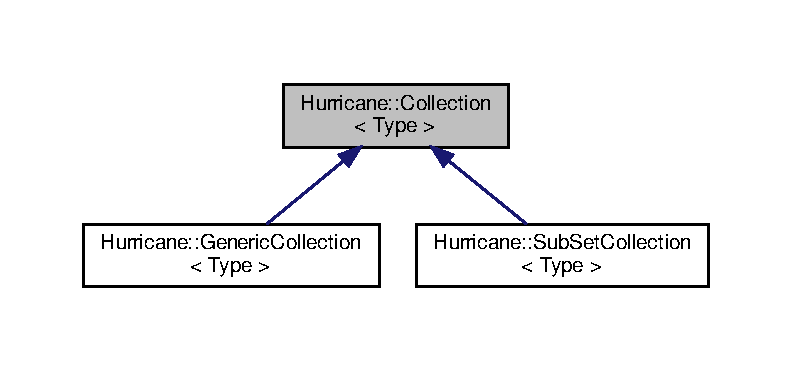
\includegraphics[width=350pt]{classHurricane_1_1Collection__inherit__graph}
\end{center}
\end{figure}
\doxysubsection*{Public Member Functions}
\begin{DoxyCompactItemize}
\item 
virtual \mbox{\hyperlink{classHurricane_1_1Collection_aafcf8e05658e245b2a762baa7a59f281}{$\sim$\+Collection}} ()
\item 
virtual \mbox{\hyperlink{classHurricane_1_1Collection}{Collection}}$<$ Type $>$ $\ast$ \mbox{\hyperlink{classHurricane_1_1Collection_ac75b91d3952b36e14f21174958523924}{get\+Clone}} () const =0
\item 
virtual \mbox{\hyperlink{classHurricane_1_1Locator}{Locator}}$<$ Type $>$ $\ast$ \mbox{\hyperlink{classHurricane_1_1Collection_a48fd1a0a2b6d2530a87e22ba65aa3152}{get\+Locator}} () const =0
\item 
virtual unsigned \mbox{\hyperlink{classHurricane_1_1Collection_a1292aabe88c9aadfdfe21dabddb62c19}{get\+Size}} () const
\item 
Type \mbox{\hyperlink{classHurricane_1_1Collection_a846a042646e02a0f77d2ce0f6190288a}{get\+First}} () const
\item 
\mbox{\hyperlink{classHurricane_1_1GenericCollection}{Generic\+Collection}}$<$ Type $>$ \mbox{\hyperlink{classHurricane_1_1Collection_aa32ea7249d57ee05e3c71dcde8106832}{get\+Sub\+Set}} (const \mbox{\hyperlink{classHurricane_1_1Filter}{Filter}}$<$ Type $>$ \&filter) const
\item 
{\footnotesize template$<$class Sub\+Type $>$ }\\\mbox{\hyperlink{classHurricane_1_1GenericCollection}{Generic\+Collection}}$<$ Sub\+Type $>$ \mbox{\hyperlink{classHurricane_1_1Collection_a91d986e21395d4021d927e06f204ab6c}{get\+Sub\+Set}} () const
\item 
{\footnotesize template$<$class Sub\+Type $>$ }\\\mbox{\hyperlink{classHurricane_1_1GenericCollection}{Generic\+Collection}}$<$ Sub\+Type $>$ \mbox{\hyperlink{classHurricane_1_1Collection_a673afd14782da82ad03a68366ae1f09b}{get\+Sub\+Set}} (const \mbox{\hyperlink{classHurricane_1_1Filter}{Filter}}$<$ Sub\+Type $>$ \&filter) const
\end{DoxyCompactItemize}


\doxysubsection{Detailed Description}
\subsubsection*{template$<$class Type$>$\newline
class Hurricane\+::\+Collection$<$ Type $>$}

\mbox{\hyperlink{classHurricane_1_1Collection}{Collection}} description ({\bfseries{API}}) 

\hypertarget{classHurricane_1_1Collection_secCollectionIntro}{}\doxysubsection{Introduction}\label{classHurricane_1_1Collection_secCollectionIntro}
Collections introduce the concept of set of elements.

Strictly speaking collections are not containers (in the STL way) but indeed set descriptors. For example, the set of instances called by a cell, which are located within a given rectangular area, will be a subtype of \mbox{\hyperlink{classHurricane_1_1Collection}{Collection}}$<$Instance$\ast$$>$ whose first attribute will be a pointer to the cell and a second attribute the rectangular area.

Main characteristics of Collections\+: 
\begin{DoxyItemize}
\item Collections {\bfseries{do not own}} their elements (they remains when the \mbox{\hyperlink{classHurricane_1_1Collection}{Collection}} is deleted). 
\item They can only be iterated {\itshape forward}. Once an element is consumed you cannot go back to it. You must restart the collection walktrough instead. 
\item Collections are very light objects which are built, copied or destroyed very rapidly. 
\end{DoxyItemize}\hypertarget{classHurricane_1_1Collection_secIterator}{}\doxysubsection{STL Iterator Support}\label{classHurricane_1_1Collection_secIterator}
The Collections now provides a basic iterator support to allow the C++11 {\ttfamily for} contruct\+: 
\begin{DoxyCode}{0}
\DoxyCodeLine{Cell* cell = ...; \textcolor{comment}{// Get a Cell from somewhere.}}
\DoxyCodeLine{}
\DoxyCodeLine{\textcolor{keywordflow}{for}( Net* inet : cell-\/>getNets() ) \{}
\DoxyCodeLine{  cout << \textcolor{stringliteral}{"{}This is "{}} << inet;}
\DoxyCodeLine{  \textcolor{keywordflow}{if} (inet-\/>isExternal())}
\DoxyCodeLine{    cout << \textcolor{stringliteral}{"{} [external net]."{}};}
\DoxyCodeLine{  cout << endl;}
\DoxyCodeLine{\}}

\end{DoxyCode}
 Although the {\ttfamily for\+Each} macro is still retained for backward compatibility, it is advisable to use the C++11 way.\hypertarget{classHurricane_1_1Collection_secForEachMacro}{}\doxysubsection{The for\+Each Macro (obsoleted)}\label{classHurricane_1_1Collection_secForEachMacro}
Collections are to be used in conjunction with the {\ttfamily for\+Each} macro which allows to easily iterate over the elements. Iteration is done through a simplistic iterator which have overload for the {\ttfamily operator$\ast$()} and {\ttfamily operator-\/$>$()}

The {\ttfamily for\+Each} macro takes three arguments\+: \begin{center} \tabulinesep=1mm
\begin{longtabu}spread 0pt [c]{*{2}{|X[-1]}|}
\hline
\multicolumn{2}{|l|}{\cellcolor{\tableheadbgcolor}\textbf{ {\ttfamily for\+Each(type,iterator,collection)} }}\\\cline{1-2}
\endfirsthead
\hline
\endfoot
\hline
\multicolumn{2}{|l|}{\cellcolor{\tableheadbgcolor}\textbf{ {\ttfamily for\+Each(type,iterator,collection)} }}\\\cline{1-2}
\endhead
{\ttfamily type} &Element\textquotesingle{}s type of the collection. \\\cline{1-2}
{\ttfamily iterator} &\mbox{\hyperlink{classHurricane_1_1Name}{Name}} of the iterator\textquotesingle{}s variable. \\\cline{1-2}
{\ttfamily collection} &An appropriate collection to iterate over, that is, built over {\ttfamily type} elements. \\\cline{1-2}
\end{longtabu}
\end{center} 

To use the for\+Each macro outside the \mbox{\hyperlink{namespaceHurricane}{Hurricane}} namespace, the following statement is necessary\+: 
\begin{DoxyCode}{0}
\DoxyCodeLine{\textcolor{keyword}{using} Hurricane::ForEachIterator}

\end{DoxyCode}
 Here is a small example of a loop\+: 
\begin{DoxyCode}{0}
\DoxyCodeLine{\textcolor{keyword}{using} Hurricane::ForEachIterator;}
\DoxyCodeLine{}
\DoxyCodeLine{Cell* cell = ...; \textcolor{comment}{// Get a Cell from somewhere.}}
\DoxyCodeLine{}
\DoxyCodeLine{forEach( Net*, inet, cell-\/>getNets() ) \{}
\DoxyCodeLine{  cout << \textcolor{stringliteral}{"{}This is "{}} << (*inet);}
\DoxyCodeLine{  \textcolor{keywordflow}{if} (inet-\/>isExternal())}
\DoxyCodeLine{    cout << \textcolor{stringliteral}{"{} [external net]."{}};}
\DoxyCodeLine{  cout << endl;}
\DoxyCodeLine{\}}

\end{DoxyCode}
\hypertarget{classHurricane_1_1Collection_secGenericgetCollection}{}\doxysubsection{The Generic get\+Collection}\label{classHurricane_1_1Collection_secGenericgetCollection}
The collections provide the generic {\ttfamily get\+Collection()} function which allows to convert its argument into a generic collection. It has no specific interest for \mbox{\hyperlink{namespaceHurricane}{Hurricane}} collections, but this function is overloaded for STL containers.

This allows to handle a STL containers like a normal collection as shown in the following example\+: 
\begin{DoxyCode}{0}
\DoxyCodeLine{set<Instance*> instanceSet;}
\DoxyCodeLine{ }
\DoxyCodeLine{\textcolor{comment}{// here we fill the set with the desired instances... }}
\DoxyCodeLine{ }
\DoxyCodeLine{forEach(Instance*, iinstance, getCollection(instanceSet)) \{}
\DoxyCodeLine{   \textcolor{comment}{// process here each instance of the set}}
\DoxyCodeLine{   \textcolor{comment}{// (the elements are visited according to the set ordering)}}
\DoxyCodeLine{\}}

\end{DoxyCode}


\begin{DoxyRemark}{Remarks}
This approach is a little bit less efficient than the use of STL iterators, not much indeed, but has the advantage to be homogeneous with the remaining code (recall\+: the created collection doesn\textquotesingle{}t make a copy of the STL container and its creation time is negligible).
\end{DoxyRemark}
\begin{DoxyParagraph}{Caution\+: The returned collection is valid whenever the STL container }
is valid. Then you should not do the following\+: 
\begin{DoxyCode}{0}
\DoxyCodeLine{GenericCollection<Instance*> getInstances(...)}
\DoxyCodeLine{\{}
\DoxyCodeLine{   set<Instance*> instanceSet;}
\DoxyCodeLine{ }
\DoxyCodeLine{   \textcolor{comment}{// we fill the container with the appropriate instances}}
\DoxyCodeLine{ }
\DoxyCodeLine{   \textcolor{keywordflow}{return} getCollection(instanceSet); \textcolor{comment}{// instanceSet deleted after return}}
\DoxyCodeLine{\}}

\end{DoxyCode}

\end{DoxyParagraph}
The same will occur anyway if you do\+: 
\begin{DoxyCode}{0}
\DoxyCodeLine{Cell* cell = ...; \textcolor{comment}{// we get the cell}}
\DoxyCodeLine{ }
\DoxyCodeLine{\mbox{\hyperlink{namespaceHurricane_a3404a8b17130a1824f4a281704b04df7}{Nets}} nets = cell-\/>getNets();}
\DoxyCodeLine{ }
\DoxyCodeLine{cell-\/>destroy();}
\DoxyCodeLine{ }
\DoxyCodeLine{forEach(Net*, inet, nets) \{}
\DoxyCodeLine{   ...}
\DoxyCodeLine{\}}

\end{DoxyCode}
\hypertarget{classHurricane_1_1Collection_secCollectionLocators}{}\doxysubsection{Locators}\label{classHurricane_1_1Collection_secCollectionLocators}
Each type of collection provides an associated \mbox{\hyperlink{classHurricane_1_1Locator}{Locator}} for tracing through the corresponding set of elements.

Each locator moves efficiently through the data structure without building (in the form of a list or any other container type) the set of elements defined by the collection (it may however use a stack (or something else) to manage recursive traces).

The elements are therefore visited in the order with which they are internally stored. No assumptions must be made about this ordering. However, collections representing an STL container are visited in the same order than the container\textquotesingle{}s one.

If you need to visit the objects in a given order, you must first fill a STL container\+: either a vector to be sorted accordingly or a set with the given sort criteria (see the Fill method below). 

\doxysubsection{Constructor \& Destructor Documentation}
\mbox{\Hypertarget{classHurricane_1_1Collection_aafcf8e05658e245b2a762baa7a59f281}\label{classHurricane_1_1Collection_aafcf8e05658e245b2a762baa7a59f281}} 
\index{Hurricane::Collection$<$ Type $>$@{Hurricane::Collection$<$ Type $>$}!````~Collection@{$\sim$Collection}}
\index{````~Collection@{$\sim$Collection}!Hurricane::Collection$<$ Type $>$@{Hurricane::Collection$<$ Type $>$}}
\doxysubsubsection{\texorpdfstring{$\sim$Collection()}{~Collection()}}
{\footnotesize\ttfamily template$<$class Type $>$ \\
\mbox{\hyperlink{classHurricane_1_1Collection}{Hurricane\+::\+Collection}}$<$ Type $>$\+::$\sim$\mbox{\hyperlink{classHurricane_1_1Collection}{Collection}}$<$ Type $>$ (\begin{DoxyParamCaption}{ }\end{DoxyParamCaption})\hspace{0.3cm}{\ttfamily [inline]}, {\ttfamily [virtual]}}

Destroys the collection but doesn\textquotesingle{}t acts on elements refered by this collection. 

\doxysubsection{Member Function Documentation}
\mbox{\Hypertarget{classHurricane_1_1Collection_ac75b91d3952b36e14f21174958523924}\label{classHurricane_1_1Collection_ac75b91d3952b36e14f21174958523924}} 
\index{Hurricane::Collection$<$ Type $>$@{Hurricane::Collection$<$ Type $>$}!getClone@{getClone}}
\index{getClone@{getClone}!Hurricane::Collection$<$ Type $>$@{Hurricane::Collection$<$ Type $>$}}
\doxysubsubsection{\texorpdfstring{getClone()}{getClone()}}
{\footnotesize\ttfamily template$<$class Type $>$ \\
\mbox{\hyperlink{classHurricane_1_1Collection}{Collection}}$<$ Type $>$ $\ast$ \mbox{\hyperlink{classHurricane_1_1Collection}{Hurricane\+::\+Collection}}$<$ Type $>$\+::get\+Clone (\begin{DoxyParamCaption}{ }\end{DoxyParamCaption}) const\hspace{0.3cm}{\ttfamily [pure virtual]}}

Allocates and returns a clone (copy) of the collection (whatever be its type).

\begin{DoxyRemark}{Remarks}
In principle there is no need to use this function. However, if you do so, don\textquotesingle{}t forget to delete the clone after use. It is indeed much easier to use generic collections which do that for you, as we will see later. 
\end{DoxyRemark}
\mbox{\Hypertarget{classHurricane_1_1Collection_a48fd1a0a2b6d2530a87e22ba65aa3152}\label{classHurricane_1_1Collection_a48fd1a0a2b6d2530a87e22ba65aa3152}} 
\index{Hurricane::Collection$<$ Type $>$@{Hurricane::Collection$<$ Type $>$}!getLocator@{getLocator}}
\index{getLocator@{getLocator}!Hurricane::Collection$<$ Type $>$@{Hurricane::Collection$<$ Type $>$}}
\doxysubsubsection{\texorpdfstring{getLocator()}{getLocator()}}
{\footnotesize\ttfamily template$<$class Type $>$ \\
\mbox{\hyperlink{classHurricane_1_1Locator}{Locator}}$<$ Type $>$ $\ast$ \mbox{\hyperlink{classHurricane_1_1Collection}{Hurricane\+::\+Collection}}$<$ Type $>$\+::get\+Locator (\begin{DoxyParamCaption}{ }\end{DoxyParamCaption}) const\hspace{0.3cm}{\ttfamily [pure virtual]}}

Allocates and returns a locator adapted to visit the elements of the collection.

\begin{DoxyRemark}{Remarks}
In principle there is no need to use this function. Use preferably the macro {\bfseries{for\+\_\+each}} described below. However, if you do so, don\textquotesingle{}t forget to delete this locator after use, else use generic locators, which do that for you, as we will see later. 
\end{DoxyRemark}


Referenced by Hurricane\+::\+Collection$<$ Type $>$\+::get\+First(), and Hurricane\+::\+Collection$<$ Type $>$\+::get\+Size().

\mbox{\Hypertarget{classHurricane_1_1Collection_a1292aabe88c9aadfdfe21dabddb62c19}\label{classHurricane_1_1Collection_a1292aabe88c9aadfdfe21dabddb62c19}} 
\index{Hurricane::Collection$<$ Type $>$@{Hurricane::Collection$<$ Type $>$}!getSize@{getSize}}
\index{getSize@{getSize}!Hurricane::Collection$<$ Type $>$@{Hurricane::Collection$<$ Type $>$}}
\doxysubsubsection{\texorpdfstring{getSize()}{getSize()}}
{\footnotesize\ttfamily template$<$class Type $>$ \\
unsigned \mbox{\hyperlink{classHurricane_1_1Collection}{Hurricane\+::\+Collection}}$<$ Type $>$\+::get\+Size (\begin{DoxyParamCaption}{ }\end{DoxyParamCaption}) const\hspace{0.3cm}{\ttfamily [inline]}, {\ttfamily [virtual]}}

{\bfseries{Returns\+:}} the number of objects identified within the collection.

\begin{DoxyRemark}{Remarks}
Very fast in some cases, but may need to visit the collection in most ones. 
\end{DoxyRemark}


References Hurricane\+::\+Collection$<$ Type $>$\+::get\+Locator().

\mbox{\Hypertarget{classHurricane_1_1Collection_a846a042646e02a0f77d2ce0f6190288a}\label{classHurricane_1_1Collection_a846a042646e02a0f77d2ce0f6190288a}} 
\index{Hurricane::Collection$<$ Type $>$@{Hurricane::Collection$<$ Type $>$}!getFirst@{getFirst}}
\index{getFirst@{getFirst}!Hurricane::Collection$<$ Type $>$@{Hurricane::Collection$<$ Type $>$}}
\doxysubsubsection{\texorpdfstring{getFirst()}{getFirst()}}
{\footnotesize\ttfamily template$<$class Type $>$ \\
Type \mbox{\hyperlink{classHurricane_1_1Collection}{Hurricane\+::\+Collection}}$<$ Type $>$\+::get\+First (\begin{DoxyParamCaption}{ }\end{DoxyParamCaption}) const\hspace{0.3cm}{\ttfamily [inline]}}

{\bfseries{Returns\+:}} the first element of the collection.

\begin{DoxyRemark}{Remarks}
The result is meaningful only when the collection is non empty. 
\end{DoxyRemark}


References Hurricane\+::\+Collection$<$ Type $>$\+::get\+Locator().

\mbox{\Hypertarget{classHurricane_1_1Collection_aa32ea7249d57ee05e3c71dcde8106832}\label{classHurricane_1_1Collection_aa32ea7249d57ee05e3c71dcde8106832}} 
\index{Hurricane::Collection$<$ Type $>$@{Hurricane::Collection$<$ Type $>$}!getSubSet@{getSubSet}}
\index{getSubSet@{getSubSet}!Hurricane::Collection$<$ Type $>$@{Hurricane::Collection$<$ Type $>$}}
\doxysubsubsection{\texorpdfstring{getSubSet()}{getSubSet()}\hspace{0.1cm}{\footnotesize\ttfamily [1/3]}}
{\footnotesize\ttfamily template$<$class Type $>$ \\
\mbox{\hyperlink{classHurricane_1_1GenericCollection}{Generic\+Collection}}$<$ Type $>$ \mbox{\hyperlink{classHurricane_1_1Collection}{Hurricane\+::\+Collection}}$<$ Type $>$\+::get\+Sub\+Set (\begin{DoxyParamCaption}\item[{const \mbox{\hyperlink{classHurricane_1_1Filter}{Filter}}$<$ Type $>$ \&}]{filter }\end{DoxyParamCaption}) const\hspace{0.3cm}{\ttfamily [inline]}}

{\bfseries{Returns\+:}} the collection representing the subset of elements accepted by the filter. 
\begin{DoxyCode}{0}
\DoxyCodeLine{\mbox{\hyperlink{namespaceHurricane_a3404a8b17130a1824f4a281704b04df7}{Nets}} \mbox{\hyperlink{classHurricane_1_1Cell_aa80f3345db8c1395fa04a50737208793}{Cell::getExternalNets}}()\textcolor{keyword}{ const}}
\DoxyCodeLine{\textcolor{keyword}{}\{}
\DoxyCodeLine{   \textcolor{keywordflow}{return} getNets().\mbox{\hyperlink{classHurricane_1_1Collection_aa32ea7249d57ee05e3c71dcde8106832}{getSubSet}}(\mbox{\hyperlink{classHurricane_1_1Net_a3af91a80e219e37e70229e61dfd385da}{Net::getIsExternalFilter}}());}
\DoxyCodeLine{\}}

\end{DoxyCode}
 \mbox{\Hypertarget{classHurricane_1_1Collection_a91d986e21395d4021d927e06f204ab6c}\label{classHurricane_1_1Collection_a91d986e21395d4021d927e06f204ab6c}} 
\index{Hurricane::Collection$<$ Type $>$@{Hurricane::Collection$<$ Type $>$}!getSubSet@{getSubSet}}
\index{getSubSet@{getSubSet}!Hurricane::Collection$<$ Type $>$@{Hurricane::Collection$<$ Type $>$}}
\doxysubsubsection{\texorpdfstring{getSubSet()}{getSubSet()}\hspace{0.1cm}{\footnotesize\ttfamily [2/3]}}
{\footnotesize\ttfamily template$<$class Type $>$ \\
template$<$class Sub\+Type $>$ \\
\mbox{\hyperlink{classHurricane_1_1GenericCollection}{Generic\+Collection}}$<$ Sub\+Type $>$ \mbox{\hyperlink{classHurricane_1_1Collection}{Hurricane\+::\+Collection}}$<$ Type $>$\+::get\+Sub\+Set$<$ Sub\+Type $>$ (\begin{DoxyParamCaption}{ }\end{DoxyParamCaption}) const\hspace{0.3cm}{\ttfamily [inline]}}

{\bfseries{Returns\+:}} the collection corresponding to the subset of elements of type {\ttfamily $<$Sub\+Type$>$}.

\begin{DoxyRemark}{Remarks}
The returned collection is a collection of objects of type {\bfseries{Sub\+Type}} and not of type {\bfseries{Type}}.
\end{DoxyRemark}

\begin{DoxyCode}{0}
\DoxyCodeLine{\mbox{\hyperlink{namespaceHurricane_a1e6a8ab09f688509bd727b3fee02d0d2}{Contacts}} \mbox{\hyperlink{classHurricane_1_1Net_a9c397596fe9ecbf674712c72e0b9010c}{Net::getContacts}}()\textcolor{keyword}{ const}}
\DoxyCodeLine{\textcolor{keyword}{}\{}
\DoxyCodeLine{   \textcolor{keywordflow}{return} getComponents().\mbox{\hyperlink{classHurricane_1_1Collection_aa32ea7249d57ee05e3c71dcde8106832}{getSubSet}}<Contact*>();}
\DoxyCodeLine{\}}

\end{DoxyCode}
 \mbox{\Hypertarget{classHurricane_1_1Collection_a673afd14782da82ad03a68366ae1f09b}\label{classHurricane_1_1Collection_a673afd14782da82ad03a68366ae1f09b}} 
\index{Hurricane::Collection$<$ Type $>$@{Hurricane::Collection$<$ Type $>$}!getSubSet@{getSubSet}}
\index{getSubSet@{getSubSet}!Hurricane::Collection$<$ Type $>$@{Hurricane::Collection$<$ Type $>$}}
\doxysubsubsection{\texorpdfstring{getSubSet()}{getSubSet()}\hspace{0.1cm}{\footnotesize\ttfamily [3/3]}}
{\footnotesize\ttfamily template$<$class Type $>$ \\
template$<$class Sub\+Type $>$ \\
\mbox{\hyperlink{classHurricane_1_1GenericCollection}{Generic\+Collection}}$<$ Sub\+Type $>$ \mbox{\hyperlink{classHurricane_1_1Collection}{Hurricane\+::\+Collection}}$<$ Type $>$\+::get\+Sub\+Set$<$ Sub\+Type $>$ (\begin{DoxyParamCaption}\item[{const \mbox{\hyperlink{classHurricane_1_1Filter}{Filter}}$<$ Sub\+Type $>$ \&}]{filter }\end{DoxyParamCaption}) const\hspace{0.3cm}{\ttfamily [inline]}}

{\bfseries{Returns\+:}} the collection representing the subset of elements of type {\ttfamily $<$Sub\+Type$>$} accepted by the filter.

\begin{DoxyRemark}{Remarks}
The returned collection is a collection of elements of type {\bfseries{Sub\+Type}} and not of type {\bfseries{Type}} and the filter must be a filter of elements of type {\bfseries{Sub\+Type}}.
\end{DoxyRemark}
\begin{DoxyParagraph}{Sample\+:\textbackslash{}n Filter Hurricane\+::Segment according to their Layer.}

\begin{DoxyCode}{0}
\DoxyCodeLine{\textcolor{keyword}{class }IsOnLayer : \textcolor{keyword}{public} Filter<Segment*> \{}
\DoxyCodeLine{   \textcolor{keyword}{public}:}
\DoxyCodeLine{      Layer* \_layer;}
\DoxyCodeLine{   \textcolor{keyword}{public}:}
\DoxyCodeLine{      IsOnLayer(Layer* layer)}
\DoxyCodeLine{        : \_layer(layer)}
\DoxyCodeLine{      \{}
\DoxyCodeLine{         \textcolor{keywordflow}{if} (!\_layer) \textcolor{keywordflow}{throw} Error(\textcolor{stringliteral}{"{}Can't create IsOnLayer filter : null layer"{}});}
\DoxyCodeLine{      \};}
\DoxyCodeLine{ }
\DoxyCodeLine{      IsOnLayer(\textcolor{keyword}{const} IsOnLayer\& isOnLayer)}
\DoxyCodeLine{        : \_layer(isOnLayer.\_layer)}
\DoxyCodeLine{      \{ \};}
\DoxyCodeLine{ }
\DoxyCodeLine{      IsOnLayer\& operator=(\textcolor{keyword}{const} IsOnLayer\& isOnLayer)}
\DoxyCodeLine{      \{}
\DoxyCodeLine{         \_layer = isOnLayer.\_layer;}
\DoxyCodeLine{         \textcolor{keywordflow}{return} *\textcolor{keyword}{this};}
\DoxyCodeLine{      \};}
\DoxyCodeLine{ }
\DoxyCodeLine{      \textcolor{keyword}{virtual} Filter<Net*>* \mbox{\hyperlink{classHurricane_1_1Collection_ac75b91d3952b36e14f21174958523924}{getClone}}()\textcolor{keyword}{ const}}
\DoxyCodeLine{\textcolor{keyword}{      }\{}
\DoxyCodeLine{         \textcolor{keywordflow}{return} \textcolor{keyword}{new} IsOnLayer(*\textcolor{keyword}{this});}
\DoxyCodeLine{      \};}
\DoxyCodeLine{ }
\DoxyCodeLine{      \textcolor{keyword}{virtual} \textcolor{keywordtype}{bool} Accept(Segment* segment)\textcolor{keyword}{ const}}
\DoxyCodeLine{\textcolor{keyword}{      }\{}
\DoxyCodeLine{         \textcolor{keywordflow}{return} (segmentgetLayer() == \_layer);}
\DoxyCodeLine{      \};}
\DoxyCodeLine{\};}

\end{DoxyCode}

\end{DoxyParagraph}
And somewher later\+: 
\begin{DoxyCode}{0}
\DoxyCodeLine{Layer* metal = getDataBase()-\/>getTechnology()-\/>getLayer(\textcolor{stringliteral}{"{}metal"{}});}
\DoxyCodeLine{ }
\DoxyCodeLine{\mbox{\hyperlink{namespaceHurricane_a30748fa53a81cb597d4a13d651238716}{Segments}} segments = net-\/>getComponents()-\/>getSubSet<Segment*>(IsOnLayer(metal));}
\DoxyCodeLine{ }
\DoxyCodeLine{\textcolor{comment}{// segments represents here the subset of net components}}
\DoxyCodeLine{\textcolor{comment}{// which are of type Segment and located on layer metal}}

\end{DoxyCode}
 

The documentation for this class was generated from the following files\+:\begin{DoxyCompactItemize}
\item 
Collection.\+h\item 
Collection.\+dox\end{DoxyCompactItemize}

\hypertarget{classEntity_1_1CompareById}{}\doxysection{Compare\+By\+Id Class Reference}
\label{classEntity_1_1CompareById}\index{CompareById@{CompareById}}


Entity comparison criterion for STL container.  




\doxysubsection{Detailed Description}
Entity comparison criterion for STL container. 

This class is a functor to be used in STL containers of {\ttfamily Entity$\ast$} whenever determinism is required (as an alternative to the object\textquotesingle{}s pointer). If a {\ttfamily NULL} pointer is passed as argument, it\textquotesingle{}s {\ttfamily id} is computed as zero, it is a failsafe and should be avoided.


\begin{DoxyCode}{0}
\DoxyCodeLine{\textcolor{keyword}{typedef}  std::map<Net*,SomeValue,Entity::CompareById>  NetMap;}
\DoxyCodeLine{}
\DoxyCodeLine{NetMap  netMap;}
\DoxyCodeLine{forEach( Net*, inet, cell-\/>getNets() ) \{}
\DoxyCodeLine{  netMap.insert( std::make\_pair(*inet,computeSomeValue(*inet)) );}
\DoxyCodeLine{\}}
\DoxyCodeLine{}
\DoxyCodeLine{\textcolor{keywordflow}{for} ( NetMap::iterator imap=netMap.begin() ; imap!=netMap.end() ; ++imap ) \{}
\DoxyCodeLine{  \textcolor{comment}{// Show the Net ordering}}
\DoxyCodeLine{  cout << (*imap).first-\/>getId() << \textcolor{stringliteral}{"{}:"{}} << (*imap).first << endl;}
\DoxyCodeLine{  \textcolor{comment}{// Do something}}
\DoxyCodeLine{  \textcolor{comment}{// ...}}
\DoxyCodeLine{\}}

\end{DoxyCode}
 

The documentation for this class was generated from the following file\+:\begin{DoxyCompactItemize}
\item 
Entity.\+dox\end{DoxyCompactItemize}

\hypertarget{classHurricane_1_1Component}{}\doxysection{Hurricane\+::Component Class Reference}
\label{classHurricane_1_1Component}\index{Hurricane::Component@{Hurricane::Component}}


\mbox{\hyperlink{classHurricane_1_1Component}{Component}} description ({\bfseries{API}})  




Inheritance diagram for Hurricane\+::Component\+:\nopagebreak
\begin{figure}[H]
\begin{center}
\leavevmode
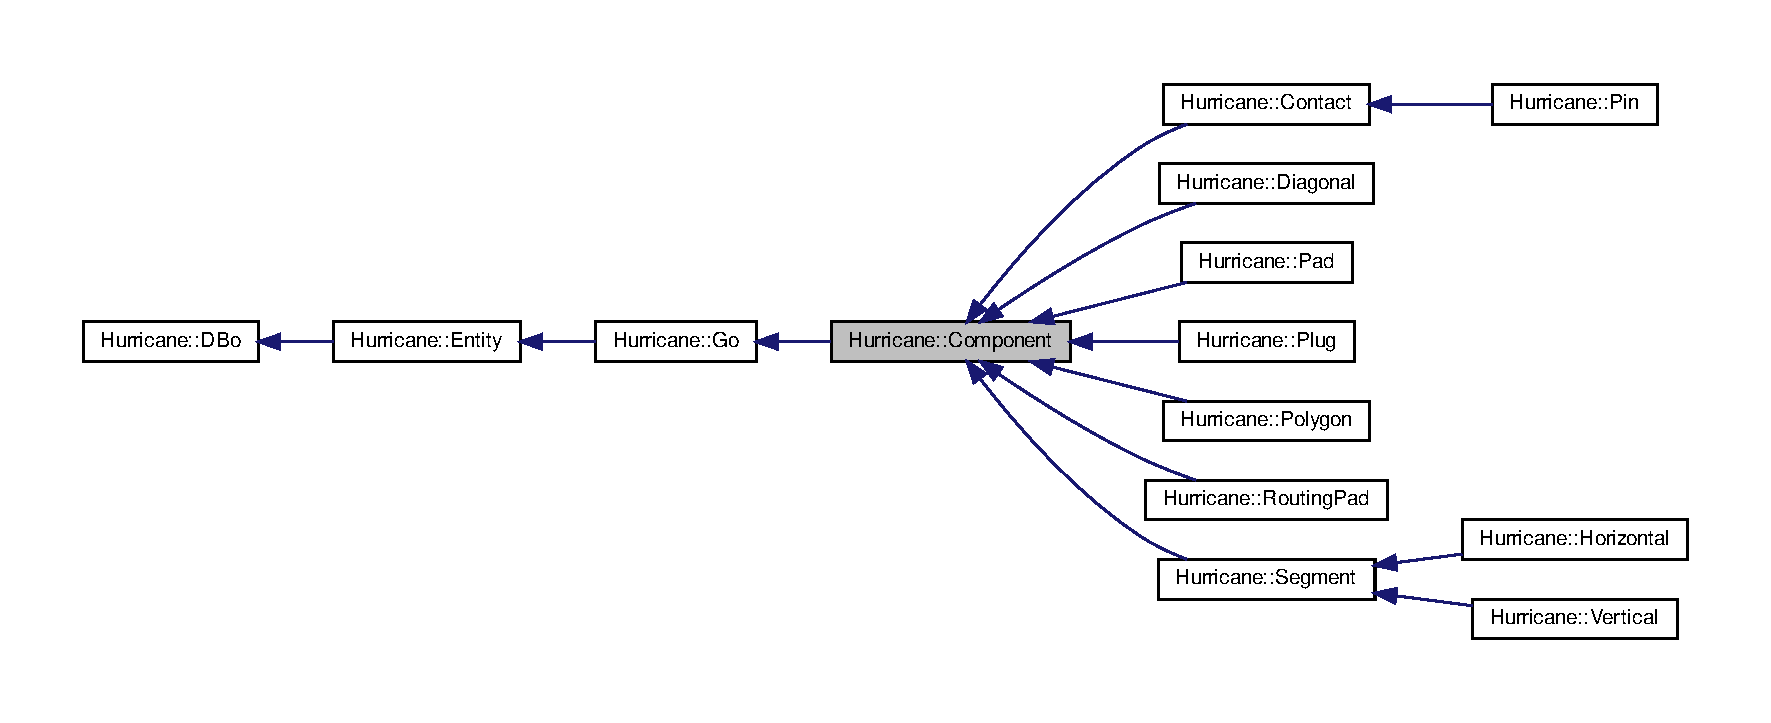
\includegraphics[width=350pt]{classHurricane_1_1Component__inherit__graph}
\end{center}
\end{figure}
\doxysubsection*{Classes}
\begin{DoxyCompactItemize}
\item 
class \mbox{\hyperlink{classHurricane_1_1Component_1_1BodyHook}{Body\+Hook}}
\end{DoxyCompactItemize}
\doxysubsection*{Public Types}
\begin{DoxyCompactItemize}
\item 
typedef \mbox{\hyperlink{classHurricane_1_1Go}{Go}} \mbox{\hyperlink{classHurricane_1_1Component_a3911e94f9d220eb809d349b1181034e3}{Inherit}}
\end{DoxyCompactItemize}
\doxysubsection*{Public Member Functions}
\begin{DoxyCompactItemize}
\item 
\mbox{\hyperlink{classHurricane_1_1Net}{Net}} $\ast$ \mbox{\hyperlink{classHurricane_1_1Component_a1556ef77d6b89bfc17698d52ebde9791}{get\+Net}} () const
\item 
\mbox{\hyperlink{classHurricane_1_1Rubber}{Rubber}} $\ast$ \mbox{\hyperlink{classHurricane_1_1Component_ab701515debfdf1bf4142d4d917aaab1d}{get\+Rubber}} () const
\item 
\mbox{\hyperlink{classHurricane_1_1Hook}{Hook}} $\ast$ \mbox{\hyperlink{classHurricane_1_1Component_a19f06d7cad163bab3b97a13f4736c9d1}{get\+Body\+Hook}} ()
\item 
virtual \mbox{\hyperlink{namespaceHurricane_a9dcd9b74dc5e2b51bec7a13c25807e02}{Hooks}} \mbox{\hyperlink{classHurricane_1_1Component_a1fc513b9465b2b8c22f41d56bf775594}{get\+Hooks}} () const
\item 
virtual \mbox{\hyperlink{classHurricane_1_1DbU_a4fbfa3e8c89347af76c9628ea06c4146}{Db\+U\+::\+Unit}} \mbox{\hyperlink{classHurricane_1_1Component_a0f8299ed73705fd4fbf56589dcc7e074}{getX}} () const =0
\item 
virtual \mbox{\hyperlink{classHurricane_1_1DbU_a4fbfa3e8c89347af76c9628ea06c4146}{Db\+U\+::\+Unit}} \mbox{\hyperlink{classHurricane_1_1Component_a727da3f127c3a7a0a09468219f98c3e6}{getY}} () const =0
\item 
virtual \mbox{\hyperlink{classHurricane_1_1Point}{Point}} \mbox{\hyperlink{classHurricane_1_1Component_aa4e9a47c89fe701670ca34355195d519}{get\+Position}} () const
\item 
virtual const \mbox{\hyperlink{classHurricane_1_1Layer}{Layer}} $\ast$ \mbox{\hyperlink{classHurricane_1_1Component_ab451ef19059e6e5bbb77ae391d02a039}{get\+Layer}} () const =0
\item 
virtual \mbox{\hyperlink{classHurricane_1_1Box}{Box}} \mbox{\hyperlink{classHurricane_1_1Component_aabb87b9ef71f71cea681a03a6213f616}{get\+Bounding\+Box}} (const \mbox{\hyperlink{classHurricane_1_1BasicLayer}{Basic\+Layer}} $\ast$) const =0
\item 
\mbox{\hyperlink{namespaceHurricane_a7d26d99aeb5dd6d70d51bd35d2473e72}{Components}} \mbox{\hyperlink{classHurricane_1_1Component_a4acf996c03b0b94a186fad653ba578a6}{get\+Connex\+Components}} () const
\item 
\mbox{\hyperlink{namespaceHurricane_a7d26d99aeb5dd6d70d51bd35d2473e72}{Components}} \mbox{\hyperlink{classHurricane_1_1Component_af6d6b7c6b3cb18754cfa02bc5fb1e754}{get\+Slave\+Components}} () const
\end{DoxyCompactItemize}
\doxysubsection*{Static Public Member Functions}
\begin{DoxyCompactItemize}
\item 
static \mbox{\hyperlink{namespaceHurricane_acbfacb3aada84aa054e587817f204e90}{Component\+Filter}} \mbox{\hyperlink{classHurricane_1_1Component_a8680f2756892366db8642bfcfd7ce097}{get\+Is\+Under\+Filter}} (const \mbox{\hyperlink{classHurricane_1_1Box}{Box}} \&area)
\end{DoxyCompactItemize}


\doxysubsection{Detailed Description}
\mbox{\hyperlink{classHurricane_1_1Component}{Component}} description ({\bfseries{API}}) 

\hypertarget{classHurricane_1_1Component_secComponentIntro}{}\doxysubsection{Introduction}\label{classHurricane_1_1Component_secComponentIntro}
Components are the abstract objects representing the category of net components (segments, contacts, pads, plugs,...). Each component knows its net, its layer and has a \char`\"{}body\char`\"{}.\hypertarget{classHurricane_1_1Component_secComponentConceptOfLocation}{}\doxysubsection{Concept of Location}\label{classHurricane_1_1Component_secComponentConceptOfLocation}
Some components (for instance the segments) bear on contacts or other segments, more precisely they bear an extremity (the origin or the extremity), possibly through an offset on other components. The real location of the concerned part is therefore relative to the location of the component on which this part bears.

For that purpose each components must be able to return a location from which a relative calculations can be done. The methods {\bfseries{\mbox{\hyperlink{classHurricane_1_1Component_a0f8299ed73705fd4fbf56589dcc7e074}{get\+X()}}}} and {\bfseries{\mbox{\hyperlink{classHurricane_1_1Component_a727da3f127c3a7a0a09468219f98c3e6}{get\+Y()}}}} provide this information and must be overloaded for each sub-\/type of component in oder to get the desired effect.

\begin{DoxyRemark}{Remarks}
The fact that a null value is systematically returned by one of this methods means that the locations are computed relative to a null value, which is equivalent to say they are absolute values (see for instance the \mbox{\hyperlink{classHurricane_1_1Horizontal}{Horizontal}} segment whose \mbox{\hyperlink{classHurricane_1_1Component_a0f8299ed73705fd4fbf56589dcc7e074}{get\+X()}} returns always null, while \mbox{\hyperlink{classHurricane_1_1Component_a727da3f127c3a7a0a09468219f98c3e6}{get\+Y()}} return the ordinate of its axis).
\end{DoxyRemark}
\hypertarget{classHurricane_1_1Component_secComponentDestruction}{}\doxysubsection{Destruction}\label{classHurricane_1_1Component_secComponentDestruction}
When a component is destroyed, all components which are anchored on its body (through the body hook) are also destroyed. This may recursively propagate to other components anchored on the body of those last ones.

Rings are reorganized such that the connectivity remains invariant.\hypertarget{classHurricane_1_1Component_secComponentPredefinedFilters}{}\doxysubsection{Predefined filters}\label{classHurricane_1_1Component_secComponentPredefinedFilters}
{\bfseries{\mbox{\hyperlink{classHurricane_1_1Component_a8680f2756892366db8642bfcfd7ce097}{Component\+::get\+Is\+Under\+Filter}}}} 

\doxysubsection{Member Typedef Documentation}
\mbox{\Hypertarget{classHurricane_1_1Component_a3911e94f9d220eb809d349b1181034e3}\label{classHurricane_1_1Component_a3911e94f9d220eb809d349b1181034e3}} 
\index{Hurricane::Component@{Hurricane::Component}!Inherit@{Inherit}}
\index{Inherit@{Inherit}!Hurricane::Component@{Hurricane::Component}}
\doxysubsubsection{\texorpdfstring{Inherit}{Inherit}}
{\footnotesize\ttfamily \mbox{\hyperlink{classHurricane_1_1Component_a3911e94f9d220eb809d349b1181034e3}{Hurricane\+::\+Component\+::\+Inherit}}}

Useful for calling upon methods of the base class without knowing it. 

\doxysubsection{Member Function Documentation}
\mbox{\Hypertarget{classHurricane_1_1Component_a1556ef77d6b89bfc17698d52ebde9791}\label{classHurricane_1_1Component_a1556ef77d6b89bfc17698d52ebde9791}} 
\index{Hurricane::Component@{Hurricane::Component}!getNet@{getNet}}
\index{getNet@{getNet}!Hurricane::Component@{Hurricane::Component}}
\doxysubsubsection{\texorpdfstring{getNet()}{getNet()}}
{\footnotesize\ttfamily \mbox{\hyperlink{classHurricane_1_1Net}{Net}} $\ast$ Hurricane\+::\+Component\+::get\+Net (\begin{DoxyParamCaption}{ }\end{DoxyParamCaption}) const\hspace{0.3cm}{\ttfamily [inline]}}

{\bfseries{Returns\+:}} the net owning the component. 

Referenced by Hurricane\+::\+Plug\+::is\+Connected().

\mbox{\Hypertarget{classHurricane_1_1Component_ab701515debfdf1bf4142d4d917aaab1d}\label{classHurricane_1_1Component_ab701515debfdf1bf4142d4d917aaab1d}} 
\index{Hurricane::Component@{Hurricane::Component}!getRubber@{getRubber}}
\index{getRubber@{getRubber}!Hurricane::Component@{Hurricane::Component}}
\doxysubsubsection{\texorpdfstring{getRubber()}{getRubber()}}
{\footnotesize\ttfamily \mbox{\hyperlink{classHurricane_1_1Rubber}{Rubber}} $\ast$ Hurricane\+::\+Component\+::get\+Rubber (\begin{DoxyParamCaption}{ }\end{DoxyParamCaption}) const\hspace{0.3cm}{\ttfamily [inline]}}

{\bfseries{Returns\+:}} the rubber associated to the component (may be NULL). \mbox{\Hypertarget{classHurricane_1_1Component_a19f06d7cad163bab3b97a13f4736c9d1}\label{classHurricane_1_1Component_a19f06d7cad163bab3b97a13f4736c9d1}} 
\index{Hurricane::Component@{Hurricane::Component}!getBodyHook@{getBodyHook}}
\index{getBodyHook@{getBodyHook}!Hurricane::Component@{Hurricane::Component}}
\doxysubsubsection{\texorpdfstring{getBodyHook()}{getBodyHook()}}
{\footnotesize\ttfamily Net\+::\+Body\+Hook $\ast$ Hurricane\+::\+Component\+::get\+Body\+Hook (\begin{DoxyParamCaption}{ }\end{DoxyParamCaption})\hspace{0.3cm}{\ttfamily [inline]}}

{\bfseries{Returns\+:}} the hook representing the component body. \mbox{\Hypertarget{classHurricane_1_1Component_a1fc513b9465b2b8c22f41d56bf775594}\label{classHurricane_1_1Component_a1fc513b9465b2b8c22f41d56bf775594}} 
\index{Hurricane::Component@{Hurricane::Component}!getHooks@{getHooks}}
\index{getHooks@{getHooks}!Hurricane::Component@{Hurricane::Component}}
\doxysubsubsection{\texorpdfstring{getHooks()}{getHooks()}}
{\footnotesize\ttfamily \mbox{\hyperlink{namespaceHurricane_a9dcd9b74dc5e2b51bec7a13c25807e02}{Hooks}} Hurricane\+::\+Component\+::get\+Hooks (\begin{DoxyParamCaption}{ }\end{DoxyParamCaption}) const\hspace{0.3cm}{\ttfamily [virtual]}}

{\bfseries{Returns\+:}} the collection of component hooks, that is the collection of nested hooks within the component, each of them representing a part of the component. \mbox{\Hypertarget{classHurricane_1_1Component_a0f8299ed73705fd4fbf56589dcc7e074}\label{classHurricane_1_1Component_a0f8299ed73705fd4fbf56589dcc7e074}} 
\index{Hurricane::Component@{Hurricane::Component}!getX@{getX}}
\index{getX@{getX}!Hurricane::Component@{Hurricane::Component}}
\doxysubsubsection{\texorpdfstring{getX()}{getX()}}
{\footnotesize\ttfamily Unit Hurricane\+::\+Component\+::getX (\begin{DoxyParamCaption}{ }\end{DoxyParamCaption}) const\hspace{0.3cm}{\ttfamily [pure virtual]}}

{\bfseries{Returns\+:}} the abscissa of the component\textquotesingle{}s body. This abscissa is a reference base for the components anchored, through an offset, on the component\textquotesingle{}s body. 

Implemented in \mbox{\hyperlink{classHurricane_1_1RoutingPad_a5c9c00c648bd0d24e1a8b0876ab442df}{Hurricane\+::\+Routing\+Pad}}.



Referenced by get\+Position().

\mbox{\Hypertarget{classHurricane_1_1Component_a727da3f127c3a7a0a09468219f98c3e6}\label{classHurricane_1_1Component_a727da3f127c3a7a0a09468219f98c3e6}} 
\index{Hurricane::Component@{Hurricane::Component}!getY@{getY}}
\index{getY@{getY}!Hurricane::Component@{Hurricane::Component}}
\doxysubsubsection{\texorpdfstring{getY()}{getY()}}
{\footnotesize\ttfamily Unit Hurricane\+::\+Component\+::getY (\begin{DoxyParamCaption}{ }\end{DoxyParamCaption}) const\hspace{0.3cm}{\ttfamily [pure virtual]}}

{\bfseries{Returns\+:}} the ordinate of the component\textquotesingle{}s body. This ordinate is a reference base for the components anchored, through an offset, on the component\textquotesingle{}s body. 

Implemented in \mbox{\hyperlink{classHurricane_1_1RoutingPad_aede4c04a7f893b1e5478b164b6eaae2d}{Hurricane\+::\+Routing\+Pad}}.



Referenced by get\+Position().

\mbox{\Hypertarget{classHurricane_1_1Component_aa4e9a47c89fe701670ca34355195d519}\label{classHurricane_1_1Component_aa4e9a47c89fe701670ca34355195d519}} 
\index{Hurricane::Component@{Hurricane::Component}!getPosition@{getPosition}}
\index{getPosition@{getPosition}!Hurricane::Component@{Hurricane::Component}}
\doxysubsubsection{\texorpdfstring{getPosition()}{getPosition()}}
{\footnotesize\ttfamily \mbox{\hyperlink{classHurricane_1_1Point}{Point}} Hurricane\+::\+Component\+::get\+Position (\begin{DoxyParamCaption}{ }\end{DoxyParamCaption}) const\hspace{0.3cm}{\ttfamily [inline]}, {\ttfamily [virtual]}}

{\bfseries{Returns\+:}} the location of the component\textquotesingle{}s body.

This method returns, in principle, a point built from the two previous methods. As far as some similar calculations are done in both methods, it is wise to redefine the method as shown below for the \mbox{\hyperlink{classHurricane_1_1Contact}{Contact}} \+: 
\begin{DoxyCode}{0}
\DoxyCodeLine{\mbox{\hyperlink{classHurricane_1_1DbU_a4fbfa3e8c89347af76c9628ea06c4146}{DbU::Unit}} Contact::getX()\textcolor{keyword}{ const}}
\DoxyCodeLine{\textcolor{keyword}{}\{}
\DoxyCodeLine{  Component* anchor = getAnchor();}
\DoxyCodeLine{  \textcolor{keywordflow}{return} (not anchor) ? \_dx : anchor-\/>getX() + \_dx;}
\DoxyCodeLine{\}}
\DoxyCodeLine{ }
\DoxyCodeLine{}
\DoxyCodeLine{\mbox{\hyperlink{classHurricane_1_1DbU_a4fbfa3e8c89347af76c9628ea06c4146}{DbU::Unit}} Contact::getY()\textcolor{keyword}{ const}}
\DoxyCodeLine{\textcolor{keyword}{}\{}
\DoxyCodeLine{  Component* anchor = getAnchor();}
\DoxyCodeLine{  \textcolor{keywordflow}{return} (not anchor) ? \_dy : anchor-\/>getY() + \_dy;}
\DoxyCodeLine{\}}
\DoxyCodeLine{ }
\DoxyCodeLine{}
\DoxyCodeLine{Point Contact::getPosition()\textcolor{keyword}{ const}}
\DoxyCodeLine{\textcolor{keyword}{}\{}
\DoxyCodeLine{  Component* anchor = getAnchor();}
\DoxyCodeLine{  \textcolor{keywordflow}{return} (not anchor) ? Point(\_dx, \_dy)}
\DoxyCodeLine{                      : anchor-\/>\mbox{\hyperlink{classHurricane_1_1Component_aa4e9a47c89fe701670ca34355195d519}{getPosition}}().Translate(\_dx, \_dy);}
\DoxyCodeLine{\}}

\end{DoxyCode}


Indeed, contacts can possibly bear on other components through an offset defined by two attributes \+\_\+dx and \+\_\+dy. In order to compute the abscissa of a contact the component on which it bears must be found. This component named the {\bfseries{anchor}} is returned by the call to get\+Anchor(). If the component has no anchor, its coordinates are considered as absolute and the attribute \+\_\+dx gives directly its abscissa.

The method get\+Anchor() must loop through a ring in order to find the contact anchor. By overloading the function \mbox{\hyperlink{classHurricane_1_1Component_aa4e9a47c89fe701670ca34355195d519}{get\+Position()}}, only one loop will be needed. Furtermore we call directly anchor-\/$>$\mbox{\hyperlink{classHurricane_1_1Component_aa4e9a47c89fe701670ca34355195d519}{get\+Position()}} and not both anchor-\/$>$\mbox{\hyperlink{classHurricane_1_1Component_a0f8299ed73705fd4fbf56589dcc7e074}{get\+X()}} and anchor-\/$>$\mbox{\hyperlink{classHurricane_1_1Component_a727da3f127c3a7a0a09468219f98c3e6}{get\+Y()}}, this will be faster (this anchor may be anchored itself on an other component). 

References get\+X(), and get\+Y().

\mbox{\Hypertarget{classHurricane_1_1Component_ab451ef19059e6e5bbb77ae391d02a039}\label{classHurricane_1_1Component_ab451ef19059e6e5bbb77ae391d02a039}} 
\index{Hurricane::Component@{Hurricane::Component}!getLayer@{getLayer}}
\index{getLayer@{getLayer}!Hurricane::Component@{Hurricane::Component}}
\doxysubsubsection{\texorpdfstring{getLayer()}{getLayer()}}
{\footnotesize\ttfamily \mbox{\hyperlink{classHurricane_1_1Layer}{Layer}} $\ast$ Hurricane\+::\+Component\+::get\+Layer (\begin{DoxyParamCaption}{ }\end{DoxyParamCaption}) const\hspace{0.3cm}{\ttfamily [pure virtual]}}

{\bfseries{Returns\+:}} the layer on which the component is located (may return NULL for some component types like the plugs). 

Implemented in \mbox{\hyperlink{classHurricane_1_1RoutingPad_a7f1e300e4148556fa223e623738d79d4}{Hurricane\+::\+Routing\+Pad}}.

\mbox{\Hypertarget{classHurricane_1_1Component_aabb87b9ef71f71cea681a03a6213f616}\label{classHurricane_1_1Component_aabb87b9ef71f71cea681a03a6213f616}} 
\index{Hurricane::Component@{Hurricane::Component}!getBoundingBox@{getBoundingBox}}
\index{getBoundingBox@{getBoundingBox}!Hurricane::Component@{Hurricane::Component}}
\doxysubsubsection{\texorpdfstring{getBoundingBox()}{getBoundingBox()}}
{\footnotesize\ttfamily \mbox{\hyperlink{classHurricane_1_1Box}{Box}} Hurricane\+::\+Component\+::get\+Bounding\+Box (\begin{DoxyParamCaption}\item[{const \mbox{\hyperlink{classHurricane_1_1BasicLayer}{Basic\+Layer}} $\ast$}]{basic\+Layer }\end{DoxyParamCaption}) const\hspace{0.3cm}{\ttfamily [pure virtual]}}

{\bfseries{Returns\+:}} the envelope of the component for the {\ttfamily $<$basic\+Layer$>$}, that is the smallest box enclosing all layout elements located on the specified basic layer.

{\bfseries{Returns\+:}} an empty box for objects which are not physical layout ones (i.\+e. plugs) or for those which have no layout on the specified basic layer. \mbox{\Hypertarget{classHurricane_1_1Component_a4acf996c03b0b94a186fad653ba578a6}\label{classHurricane_1_1Component_a4acf996c03b0b94a186fad653ba578a6}} 
\index{Hurricane::Component@{Hurricane::Component}!getConnexComponents@{getConnexComponents}}
\index{getConnexComponents@{getConnexComponents}!Hurricane::Component@{Hurricane::Component}}
\doxysubsubsection{\texorpdfstring{getConnexComponents()}{getConnexComponents()}}
{\footnotesize\ttfamily \mbox{\hyperlink{namespaceHurricane_a7d26d99aeb5dd6d70d51bd35d2473e72}{Components}} Hurricane\+::\+Component\+::get\+Connex\+Components (\begin{DoxyParamCaption}{ }\end{DoxyParamCaption}) const}

{\bfseries{Returns\+:}} the collection of \char`\"{}connex components\char`\"{} to the component {\ttfamily $<$this$>$} (which includes at least this one).

\begin{DoxyRemark}{Remarks}
A componnent is said {\bfseries{connex}} to an other one if it is attached directly or indirectly through hyper-\/hooks, that is if there exist a sequence of components whose parts (extremities or body) are either sharing the same anchor or anchored one upon the other.
\end{DoxyRemark}
If the layout elements are correctly assembled and on the proper layers, this \char`\"{}connex components collection\char`\"{} represents an geometrically and electrically connected subset of layout elements

On the other hand, if layout anchored objects don\textquotesingle{}t overlap on the same conducting layers (either by a wrong contact layer or by an offset which forbids layout intersection) electrical continuity will not be ensured. \mbox{\Hypertarget{classHurricane_1_1Component_af6d6b7c6b3cb18754cfa02bc5fb1e754}\label{classHurricane_1_1Component_af6d6b7c6b3cb18754cfa02bc5fb1e754}} 
\index{Hurricane::Component@{Hurricane::Component}!getSlaveComponents@{getSlaveComponents}}
\index{getSlaveComponents@{getSlaveComponents}!Hurricane::Component@{Hurricane::Component}}
\doxysubsubsection{\texorpdfstring{getSlaveComponents()}{getSlaveComponents()}}
{\footnotesize\ttfamily \mbox{\hyperlink{namespaceHurricane_a7d26d99aeb5dd6d70d51bd35d2473e72}{Components}} Hurricane\+::\+Component\+::get\+Slave\+Components (\begin{DoxyParamCaption}{ }\end{DoxyParamCaption}) const}

{\bfseries{Returns\+:}} the collection of components whose existence depends directly or indirectly of the existence of the component {\ttfamily $<$this$>$} (a segment can\textquotesingle{}t survive to the destruction of a contact on which it is anchored). \mbox{\Hypertarget{classHurricane_1_1Component_a8680f2756892366db8642bfcfd7ce097}\label{classHurricane_1_1Component_a8680f2756892366db8642bfcfd7ce097}} 
\index{Hurricane::Component@{Hurricane::Component}!getIsUnderFilter@{getIsUnderFilter}}
\index{getIsUnderFilter@{getIsUnderFilter}!Hurricane::Component@{Hurricane::Component}}
\doxysubsubsection{\texorpdfstring{getIsUnderFilter()}{getIsUnderFilter()}}
{\footnotesize\ttfamily \mbox{\hyperlink{namespaceHurricane_acbfacb3aada84aa054e587817f204e90}{Component\+Filter}} Hurricane\+::\+Component\+::get\+Is\+Under\+Filter (\begin{DoxyParamCaption}\item[{const \mbox{\hyperlink{classHurricane_1_1Box}{Box}} \&}]{area }\end{DoxyParamCaption})\hspace{0.3cm}{\ttfamily [static]}}

{\bfseries{Returns\+:}} the filter allowing to select only components which intersect the rectangular {\ttfamily $<$area$>$}. 

The documentation for this class was generated from the following files\+:\begin{DoxyCompactItemize}
\item 
Component.\+h\item 
Component.\+dox\end{DoxyCompactItemize}

\hypertarget{classHurricane_1_1Contact}{}\section{Hurricane\+:\+:Contact Class Reference}
\label{classHurricane_1_1Contact}\index{Hurricane\+::\+Contact@{Hurricane\+::\+Contact}}


\mbox{\hyperlink{classHurricane_1_1Contact}{Contact}} description ({\bfseries A\+PI})  




Inheritance diagram for Hurricane\+:\+:Contact\+:\nopagebreak
\begin{figure}[H]
\begin{center}
\leavevmode
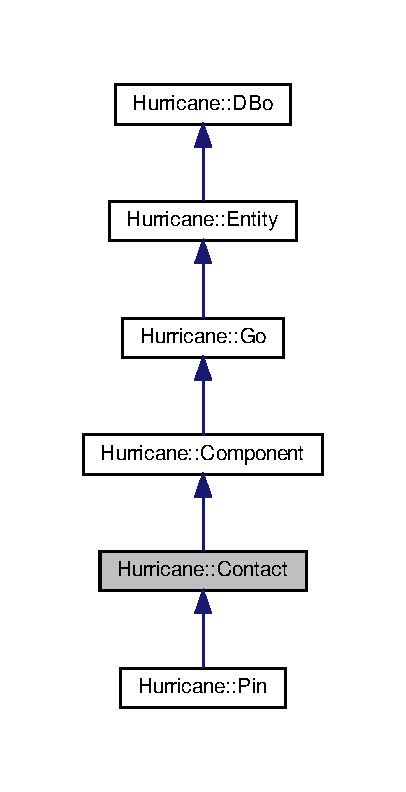
\includegraphics[width=206pt]{classHurricane_1_1Contact__inherit__graph}
\end{center}
\end{figure}
\subsection*{Classes}
\begin{DoxyCompactItemize}
\item 
class \mbox{\hyperlink{classHurricane_1_1Contact_1_1AnchorHook}{Anchor\+Hook}}
\end{DoxyCompactItemize}
\subsection*{Public Types}
\begin{DoxyCompactItemize}
\item 
typedef \mbox{\hyperlink{classHurricane_1_1Component}{Component}} \mbox{\hyperlink{classHurricane_1_1Contact_a422f15bba0561d8499c001fb8cbe6b67}{Inherit}}
\end{DoxyCompactItemize}
\subsection*{Public Member Functions}
\begin{DoxyCompactItemize}
\item 
\mbox{\hyperlink{classHurricane_1_1Hook}{Hook}} $\ast$ \mbox{\hyperlink{classHurricane_1_1Contact_a300306b006397377bc9a54ea783c1150}{get\+Anchor\+Hook}} ()
\item 
\mbox{\hyperlink{classHurricane_1_1Component}{Component}} $\ast$ \mbox{\hyperlink{classHurricane_1_1Contact_ab0b327b306bf7ebda634f59d8d0cfd8f}{get\+Anchor}} () const
\item 
\mbox{\hyperlink{group__DbUGroup_ga4fbfa3e8c89347af76c9628ea06c4146}{Db\+U\+::\+Unit}} \mbox{\hyperlink{classHurricane_1_1Contact_a8a5c4475668b6c6730ed5265e5447553}{get\+Dx}} () const
\item 
\mbox{\hyperlink{group__DbUGroup_ga4fbfa3e8c89347af76c9628ea06c4146}{Db\+U\+::\+Unit}} \mbox{\hyperlink{classHurricane_1_1Contact_af674c59fcaf1f5214d54a558fe30e41a}{get\+Dy}} () const
\item 
\mbox{\hyperlink{group__DbUGroup_ga4fbfa3e8c89347af76c9628ea06c4146}{Db\+U\+::\+Unit}} \mbox{\hyperlink{classHurricane_1_1Contact_a794ce7c3aa5ffe894c1231f7c5ac3c52}{get\+Width}} () const
\item 
\mbox{\hyperlink{group__DbUGroup_ga4fbfa3e8c89347af76c9628ea06c4146}{Db\+U\+::\+Unit}} \mbox{\hyperlink{classHurricane_1_1Contact_a4a5136f4e8299435e50db7da28172ca1}{get\+Half\+Width}} () const
\item 
\mbox{\hyperlink{group__DbUGroup_ga4fbfa3e8c89347af76c9628ea06c4146}{Db\+U\+::\+Unit}} \mbox{\hyperlink{classHurricane_1_1Contact_a07a4ecc7ea2479e2d63f5f31d9325dde}{get\+Height}} () const
\item 
\mbox{\hyperlink{group__DbUGroup_ga4fbfa3e8c89347af76c9628ea06c4146}{Db\+U\+::\+Unit}} \mbox{\hyperlink{classHurricane_1_1Contact_aebd3ff8e1368617ab750b20ae9ffb59b}{get\+Half\+Height}} () const
\item 
void \mbox{\hyperlink{classHurricane_1_1Contact_aec627634d5b6cfc5079a02b1b518b50e}{set\+Layer}} (const \mbox{\hyperlink{classHurricane_1_1Layer}{Layer}} $\ast$)
\item 
void \mbox{\hyperlink{classHurricane_1_1Contact_a08d14ce6cdf3696e472f4a621b936afe}{set\+Width}} (\mbox{\hyperlink{group__DbUGroup_ga4fbfa3e8c89347af76c9628ea06c4146}{Db\+U\+::\+Unit}})
\item 
void \mbox{\hyperlink{classHurricane_1_1Contact_a6480b6a75cc098d3227f27080a2cb42b}{set\+Height}} (\mbox{\hyperlink{group__DbUGroup_ga4fbfa3e8c89347af76c9628ea06c4146}{Db\+U\+::\+Unit}})
\item 
void \mbox{\hyperlink{classHurricane_1_1Contact_a1bded13596d448c6bb9c93271fffe5fd}{set\+Sizes}} (\mbox{\hyperlink{group__DbUGroup_ga4fbfa3e8c89347af76c9628ea06c4146}{Db\+U\+::\+Unit}} width, \mbox{\hyperlink{group__DbUGroup_ga4fbfa3e8c89347af76c9628ea06c4146}{Db\+U\+::\+Unit}} height)
\item 
void \mbox{\hyperlink{classHurricane_1_1Contact_a5b2338675993259feabb641fd9a1996e}{setX}} (\mbox{\hyperlink{group__DbUGroup_ga4fbfa3e8c89347af76c9628ea06c4146}{Db\+U\+::\+Unit}})
\item 
void \mbox{\hyperlink{classHurricane_1_1Contact_a232a49a5dd180e9ff8dfb2bd2a67f2cd}{setY}} (\mbox{\hyperlink{group__DbUGroup_ga4fbfa3e8c89347af76c9628ea06c4146}{Db\+U\+::\+Unit}})
\item 
void \mbox{\hyperlink{classHurricane_1_1Contact_ae44d4d7655428705f13dca34c7167690}{set\+Position}} (\mbox{\hyperlink{group__DbUGroup_ga4fbfa3e8c89347af76c9628ea06c4146}{Db\+U\+::\+Unit}} x, \mbox{\hyperlink{group__DbUGroup_ga4fbfa3e8c89347af76c9628ea06c4146}{Db\+U\+::\+Unit}} y)
\item 
void \mbox{\hyperlink{classHurricane_1_1Contact_aedcc63fe54538939c03fe81a16b0bae0}{set\+Position}} (const \mbox{\hyperlink{classHurricane_1_1Point}{Point}} \&)
\item 
void \mbox{\hyperlink{classHurricane_1_1Contact_a82f29c6b48b0c5a51fe3c1678d71876c}{set\+Dx}} (\mbox{\hyperlink{group__DbUGroup_ga4fbfa3e8c89347af76c9628ea06c4146}{Db\+U\+::\+Unit}})
\item 
void \mbox{\hyperlink{classHurricane_1_1Contact_ac5dadc06ae38c1ff287f031864f58850}{set\+Dy}} (\mbox{\hyperlink{group__DbUGroup_ga4fbfa3e8c89347af76c9628ea06c4146}{Db\+U\+::\+Unit}})
\item 
void \mbox{\hyperlink{classHurricane_1_1Contact_a5c8cb75debcbe10aedc092e2089a975c}{set\+Offset}} (\mbox{\hyperlink{group__DbUGroup_ga4fbfa3e8c89347af76c9628ea06c4146}{Db\+U\+::\+Unit}} dx, \mbox{\hyperlink{group__DbUGroup_ga4fbfa3e8c89347af76c9628ea06c4146}{Db\+U\+::\+Unit}} dy)
\end{DoxyCompactItemize}
\subsection*{Static Public Member Functions}
\begin{DoxyCompactItemize}
\item 
static \mbox{\hyperlink{classHurricane_1_1Contact}{Contact}} $\ast$ \mbox{\hyperlink{classHurricane_1_1Contact_ab66989c2dce4d398f1f7647aca50d983}{create}} (\mbox{\hyperlink{classHurricane_1_1Net}{Net}} $\ast$net, const \mbox{\hyperlink{classHurricane_1_1Layer}{Layer}} $\ast$layer, \mbox{\hyperlink{group__DbUGroup_ga4fbfa3e8c89347af76c9628ea06c4146}{Db\+U\+::\+Unit}} x, \mbox{\hyperlink{group__DbUGroup_ga4fbfa3e8c89347af76c9628ea06c4146}{Db\+U\+::\+Unit}} y, \mbox{\hyperlink{group__DbUGroup_ga4fbfa3e8c89347af76c9628ea06c4146}{Db\+U\+::\+Unit}} width=0, \mbox{\hyperlink{group__DbUGroup_ga4fbfa3e8c89347af76c9628ea06c4146}{Db\+U\+::\+Unit}} height=0)
\item 
static \mbox{\hyperlink{classHurricane_1_1Contact}{Contact}} $\ast$ \mbox{\hyperlink{classHurricane_1_1Contact_a2e555edb8984b599c391f16db105c1f5}{create}} (\mbox{\hyperlink{classHurricane_1_1Component}{Component}} $\ast$anchor, const \mbox{\hyperlink{classHurricane_1_1Layer}{Layer}} $\ast$layer, \mbox{\hyperlink{group__DbUGroup_ga4fbfa3e8c89347af76c9628ea06c4146}{Db\+U\+::\+Unit}} dx, \mbox{\hyperlink{group__DbUGroup_ga4fbfa3e8c89347af76c9628ea06c4146}{Db\+U\+::\+Unit}} dy, \mbox{\hyperlink{group__DbUGroup_ga4fbfa3e8c89347af76c9628ea06c4146}{Db\+U\+::\+Unit}} width=0, \mbox{\hyperlink{group__DbUGroup_ga4fbfa3e8c89347af76c9628ea06c4146}{Db\+U\+::\+Unit}} height=0)
\end{DoxyCompactItemize}


\subsection{Detailed Description}
\mbox{\hyperlink{classHurricane_1_1Contact}{Contact}} description ({\bfseries A\+PI}) 

\hypertarget{classHurricane_1_1Contact_secContactIntro}{}\subsection{Introduction}\label{classHurricane_1_1Contact_secContactIntro}
Contacts are objects representing contact points within a net. A contact may have a null size, be a single layer contact or a multi-\/layer contact (i.\+e. a V\+IA). 

\subsection{Member Typedef Documentation}
\mbox{\Hypertarget{classHurricane_1_1Contact_a422f15bba0561d8499c001fb8cbe6b67}\label{classHurricane_1_1Contact_a422f15bba0561d8499c001fb8cbe6b67}} 
\index{Hurricane\+::\+Contact@{Hurricane\+::\+Contact}!Inherit@{Inherit}}
\index{Inherit@{Inherit}!Hurricane\+::\+Contact@{Hurricane\+::\+Contact}}
\subsubsection{\texorpdfstring{Inherit}{Inherit}}
{\footnotesize\ttfamily \mbox{\hyperlink{classHurricane_1_1Contact_a422f15bba0561d8499c001fb8cbe6b67}{Hurricane\+::\+Contact\+::\+Inherit}}}

Useful for calling upon methods of the base class without knowing it. 

\subsection{Member Function Documentation}
\mbox{\Hypertarget{classHurricane_1_1Contact_ab66989c2dce4d398f1f7647aca50d983}\label{classHurricane_1_1Contact_ab66989c2dce4d398f1f7647aca50d983}} 
\index{Hurricane\+::\+Contact@{Hurricane\+::\+Contact}!create@{create}}
\index{create@{create}!Hurricane\+::\+Contact@{Hurricane\+::\+Contact}}
\subsubsection{\texorpdfstring{create()}{create()}\hspace{0.1cm}{\footnotesize\ttfamily [1/2]}}
{\footnotesize\ttfamily \mbox{\hyperlink{classHurricane_1_1Contact}{Contact}} $\ast$ Hurricane\+::\+Contact\+::create (\begin{DoxyParamCaption}\item[{\mbox{\hyperlink{classHurricane_1_1Net}{Net}} $\ast$}]{net,  }\item[{const \mbox{\hyperlink{classHurricane_1_1Layer}{Layer}} $\ast$}]{layer,  }\item[{\mbox{\hyperlink{group__DbUGroup_ga4fbfa3e8c89347af76c9628ea06c4146}{Db\+U\+::\+Unit}}}]{x,  }\item[{\mbox{\hyperlink{group__DbUGroup_ga4fbfa3e8c89347af76c9628ea06c4146}{Db\+U\+::\+Unit}}}]{y,  }\item[{\mbox{\hyperlink{group__DbUGroup_ga4fbfa3e8c89347af76c9628ea06c4146}{Db\+U\+::\+Unit}}}]{width = {\ttfamily 0},  }\item[{\mbox{\hyperlink{group__DbUGroup_ga4fbfa3e8c89347af76c9628ea06c4146}{Db\+U\+::\+Unit}}}]{height = {\ttfamily 0} }\end{DoxyParamCaption})\hspace{0.3cm}{\ttfamily [static]}}

creates and returns a new contact belonging to the net {\ttfamily $<$net$>$}, on the layer {\ttfamily $<$layer$>$}, of size {\ttfamily $<$width$>$} and {\ttfamily $<$height$>$} and located at the absolute coordinates {\ttfamily $<$x$>$} and {\ttfamily $<$y$>$}.

\begin{DoxyParagraph}{Caution\+: Throws an exception if the layer or the net is null. }

\end{DoxyParagraph}
\mbox{\Hypertarget{classHurricane_1_1Contact_a2e555edb8984b599c391f16db105c1f5}\label{classHurricane_1_1Contact_a2e555edb8984b599c391f16db105c1f5}} 
\index{Hurricane\+::\+Contact@{Hurricane\+::\+Contact}!create@{create}}
\index{create@{create}!Hurricane\+::\+Contact@{Hurricane\+::\+Contact}}
\subsubsection{\texorpdfstring{create()}{create()}\hspace{0.1cm}{\footnotesize\ttfamily [2/2]}}
{\footnotesize\ttfamily \mbox{\hyperlink{classHurricane_1_1Contact}{Contact}} $\ast$ Hurricane\+::\+Contact\+::create (\begin{DoxyParamCaption}\item[{\mbox{\hyperlink{classHurricane_1_1Component}{Component}} $\ast$}]{anchor,  }\item[{const \mbox{\hyperlink{classHurricane_1_1Layer}{Layer}} $\ast$}]{layer,  }\item[{\mbox{\hyperlink{group__DbUGroup_ga4fbfa3e8c89347af76c9628ea06c4146}{Db\+U\+::\+Unit}}}]{dx,  }\item[{\mbox{\hyperlink{group__DbUGroup_ga4fbfa3e8c89347af76c9628ea06c4146}{Db\+U\+::\+Unit}}}]{dy,  }\item[{\mbox{\hyperlink{group__DbUGroup_ga4fbfa3e8c89347af76c9628ea06c4146}{Db\+U\+::\+Unit}}}]{width = {\ttfamily 0},  }\item[{\mbox{\hyperlink{group__DbUGroup_ga4fbfa3e8c89347af76c9628ea06c4146}{Db\+U\+::\+Unit}}}]{height = {\ttfamily 0} }\end{DoxyParamCaption})\hspace{0.3cm}{\ttfamily [static]}}

creates and returns a new contact on the layer {\ttfamily $<$layer$>$}, of size {\ttfamily $<$width$>$} and {\ttfamily $<$height$>$} attached upon the component {\ttfamily $<$anchor$>$} through an offset defined by {\ttfamily $<$dx$>$} et {\ttfamily $<$dy$>$}.

\begin{DoxyParagraph}{Caution\+: Throws an exception if the layer or the anchor is null or if }
the anchor is an unconnected plug.
\end{DoxyParagraph}
\begin{DoxyRemark}{Remarks}
The new contact belongs to the anchor\textquotesingle{}s net. 
\end{DoxyRemark}
\mbox{\Hypertarget{classHurricane_1_1Contact_a300306b006397377bc9a54ea783c1150}\label{classHurricane_1_1Contact_a300306b006397377bc9a54ea783c1150}} 
\index{Hurricane\+::\+Contact@{Hurricane\+::\+Contact}!get\+Anchor\+Hook@{get\+Anchor\+Hook}}
\index{get\+Anchor\+Hook@{get\+Anchor\+Hook}!Hurricane\+::\+Contact@{Hurricane\+::\+Contact}}
\subsubsection{\texorpdfstring{get\+Anchor\+Hook()}{getAnchorHook()}}
{\footnotesize\ttfamily \mbox{\hyperlink{classHurricane_1_1Contact_1_1AnchorHook}{Contact\+::\+Anchor\+Hook}} $\ast$ Hurricane\+::\+Contact\+::get\+Anchor\+Hook (\begin{DoxyParamCaption}{ }\end{DoxyParamCaption})\hspace{0.3cm}{\ttfamily [inline]}}

{\bfseries Returns\+:} the hook through which the contact can be attached upon an anchor. \mbox{\Hypertarget{classHurricane_1_1Contact_ab0b327b306bf7ebda634f59d8d0cfd8f}\label{classHurricane_1_1Contact_ab0b327b306bf7ebda634f59d8d0cfd8f}} 
\index{Hurricane\+::\+Contact@{Hurricane\+::\+Contact}!get\+Anchor@{get\+Anchor}}
\index{get\+Anchor@{get\+Anchor}!Hurricane\+::\+Contact@{Hurricane\+::\+Contact}}
\subsubsection{\texorpdfstring{get\+Anchor()}{getAnchor()}}
{\footnotesize\ttfamily \mbox{\hyperlink{classHurricane_1_1Component}{Component}} $\ast$ Hurricane\+::\+Contact\+::get\+Anchor (\begin{DoxyParamCaption}{ }\end{DoxyParamCaption}) const}

The anchor hook of the contact being a slave one, it may have a master hook representing the body of the anchor on which it is attached. This method returns the owner of this master hook if it exists else N\+U\+LL (either the contact is an absolute one (its anchor hook is not inserted in a ring) or this ring doesn\textquotesingle{}t contain a master hook (lowly probable, transitory)). \mbox{\Hypertarget{classHurricane_1_1Contact_a8a5c4475668b6c6730ed5265e5447553}\label{classHurricane_1_1Contact_a8a5c4475668b6c6730ed5265e5447553}} 
\index{Hurricane\+::\+Contact@{Hurricane\+::\+Contact}!get\+Dx@{get\+Dx}}
\index{get\+Dx@{get\+Dx}!Hurricane\+::\+Contact@{Hurricane\+::\+Contact}}
\subsubsection{\texorpdfstring{get\+Dx()}{getDx()}}
{\footnotesize\ttfamily \mbox{\hyperlink{group__DbUGroup_ga4fbfa3e8c89347af76c9628ea06c4146}{Db\+U\+::\+Unit}} Hurricane\+::\+Contact\+::get\+Dx (\begin{DoxyParamCaption}{ }\end{DoxyParamCaption}) const\hspace{0.3cm}{\ttfamily [inline]}}

{\bfseries Returns\+:} the relative abscissa of the contact.

\begin{DoxyRemark}{Remarks}
If you want to get the absolute one use the member function get\+X() defined at the \mbox{\hyperlink{classHurricane_1_1Component}{Component}} level. 
\end{DoxyRemark}
\mbox{\Hypertarget{classHurricane_1_1Contact_af674c59fcaf1f5214d54a558fe30e41a}\label{classHurricane_1_1Contact_af674c59fcaf1f5214d54a558fe30e41a}} 
\index{Hurricane\+::\+Contact@{Hurricane\+::\+Contact}!get\+Dy@{get\+Dy}}
\index{get\+Dy@{get\+Dy}!Hurricane\+::\+Contact@{Hurricane\+::\+Contact}}
\subsubsection{\texorpdfstring{get\+Dy()}{getDy()}}
{\footnotesize\ttfamily \mbox{\hyperlink{group__DbUGroup_ga4fbfa3e8c89347af76c9628ea06c4146}{Db\+U\+::\+Unit}} Hurricane\+::\+Contact\+::get\+Dy (\begin{DoxyParamCaption}{ }\end{DoxyParamCaption}) const\hspace{0.3cm}{\ttfamily [inline]}}

{\bfseries Returns\+:} the relative ordinate of the contact.

\begin{DoxyRemark}{Remarks}
If you want to get the absolute one use the member function get\+Y() defined at the \mbox{\hyperlink{classHurricane_1_1Component}{Component}} level. 
\end{DoxyRemark}
\mbox{\Hypertarget{classHurricane_1_1Contact_a794ce7c3aa5ffe894c1231f7c5ac3c52}\label{classHurricane_1_1Contact_a794ce7c3aa5ffe894c1231f7c5ac3c52}} 
\index{Hurricane\+::\+Contact@{Hurricane\+::\+Contact}!get\+Width@{get\+Width}}
\index{get\+Width@{get\+Width}!Hurricane\+::\+Contact@{Hurricane\+::\+Contact}}
\subsubsection{\texorpdfstring{get\+Width()}{getWidth()}}
{\footnotesize\ttfamily \mbox{\hyperlink{group__DbUGroup_ga4fbfa3e8c89347af76c9628ea06c4146}{Db\+U\+::\+Unit}} Hurricane\+::\+Contact\+::get\+Width (\begin{DoxyParamCaption}{ }\end{DoxyParamCaption}) const\hspace{0.3cm}{\ttfamily [inline]}}

{\bfseries Returns\+:} the contact width. \mbox{\Hypertarget{classHurricane_1_1Contact_a4a5136f4e8299435e50db7da28172ca1}\label{classHurricane_1_1Contact_a4a5136f4e8299435e50db7da28172ca1}} 
\index{Hurricane\+::\+Contact@{Hurricane\+::\+Contact}!get\+Half\+Width@{get\+Half\+Width}}
\index{get\+Half\+Width@{get\+Half\+Width}!Hurricane\+::\+Contact@{Hurricane\+::\+Contact}}
\subsubsection{\texorpdfstring{get\+Half\+Width()}{getHalfWidth()}}
{\footnotesize\ttfamily \mbox{\hyperlink{group__DbUGroup_ga4fbfa3e8c89347af76c9628ea06c4146}{Db\+U\+::\+Unit}} Hurricane\+::\+Contact\+::get\+Half\+Width (\begin{DoxyParamCaption}{ }\end{DoxyParamCaption}) const\hspace{0.3cm}{\ttfamily [inline]}}

{\bfseries Returns\+:} the contact half width. \mbox{\Hypertarget{classHurricane_1_1Contact_a07a4ecc7ea2479e2d63f5f31d9325dde}\label{classHurricane_1_1Contact_a07a4ecc7ea2479e2d63f5f31d9325dde}} 
\index{Hurricane\+::\+Contact@{Hurricane\+::\+Contact}!get\+Height@{get\+Height}}
\index{get\+Height@{get\+Height}!Hurricane\+::\+Contact@{Hurricane\+::\+Contact}}
\subsubsection{\texorpdfstring{get\+Height()}{getHeight()}}
{\footnotesize\ttfamily \mbox{\hyperlink{group__DbUGroup_ga4fbfa3e8c89347af76c9628ea06c4146}{Db\+U\+::\+Unit}} Hurricane\+::\+Contact\+::get\+Height (\begin{DoxyParamCaption}{ }\end{DoxyParamCaption}) const\hspace{0.3cm}{\ttfamily [inline]}}

{\bfseries Returns\+:} the contact height. \mbox{\Hypertarget{classHurricane_1_1Contact_aebd3ff8e1368617ab750b20ae9ffb59b}\label{classHurricane_1_1Contact_aebd3ff8e1368617ab750b20ae9ffb59b}} 
\index{Hurricane\+::\+Contact@{Hurricane\+::\+Contact}!get\+Half\+Height@{get\+Half\+Height}}
\index{get\+Half\+Height@{get\+Half\+Height}!Hurricane\+::\+Contact@{Hurricane\+::\+Contact}}
\subsubsection{\texorpdfstring{get\+Half\+Height()}{getHalfHeight()}}
{\footnotesize\ttfamily \mbox{\hyperlink{group__DbUGroup_ga4fbfa3e8c89347af76c9628ea06c4146}{Db\+U\+::\+Unit}} Hurricane\+::\+Contact\+::get\+Half\+Height (\begin{DoxyParamCaption}{ }\end{DoxyParamCaption}) const\hspace{0.3cm}{\ttfamily [inline]}}

{\bfseries Returns\+:} the contact half height. \mbox{\Hypertarget{classHurricane_1_1Contact_aec627634d5b6cfc5079a02b1b518b50e}\label{classHurricane_1_1Contact_aec627634d5b6cfc5079a02b1b518b50e}} 
\index{Hurricane\+::\+Contact@{Hurricane\+::\+Contact}!set\+Layer@{set\+Layer}}
\index{set\+Layer@{set\+Layer}!Hurricane\+::\+Contact@{Hurricane\+::\+Contact}}
\subsubsection{\texorpdfstring{set\+Layer()}{setLayer()}}
{\footnotesize\ttfamily void Hurricane\+::\+Contact\+::set\+Layer (\begin{DoxyParamCaption}\item[{const \mbox{\hyperlink{classHurricane_1_1Layer}{Layer}} $\ast$}]{layer }\end{DoxyParamCaption})}

sets the contact layer. \mbox{\Hypertarget{classHurricane_1_1Contact_a08d14ce6cdf3696e472f4a621b936afe}\label{classHurricane_1_1Contact_a08d14ce6cdf3696e472f4a621b936afe}} 
\index{Hurricane\+::\+Contact@{Hurricane\+::\+Contact}!set\+Width@{set\+Width}}
\index{set\+Width@{set\+Width}!Hurricane\+::\+Contact@{Hurricane\+::\+Contact}}
\subsubsection{\texorpdfstring{set\+Width()}{setWidth()}}
{\footnotesize\ttfamily void Hurricane\+::\+Contact\+::set\+Width (\begin{DoxyParamCaption}\item[{\mbox{\hyperlink{group__DbUGroup_ga4fbfa3e8c89347af76c9628ea06c4146}{Db\+U\+::\+Unit}}}]{width }\end{DoxyParamCaption})}

sets the contact width. \mbox{\Hypertarget{classHurricane_1_1Contact_a6480b6a75cc098d3227f27080a2cb42b}\label{classHurricane_1_1Contact_a6480b6a75cc098d3227f27080a2cb42b}} 
\index{Hurricane\+::\+Contact@{Hurricane\+::\+Contact}!set\+Height@{set\+Height}}
\index{set\+Height@{set\+Height}!Hurricane\+::\+Contact@{Hurricane\+::\+Contact}}
\subsubsection{\texorpdfstring{set\+Height()}{setHeight()}}
{\footnotesize\ttfamily void Hurricane\+::\+Contact\+::set\+Height (\begin{DoxyParamCaption}\item[{\mbox{\hyperlink{group__DbUGroup_ga4fbfa3e8c89347af76c9628ea06c4146}{Db\+U\+::\+Unit}}}]{height }\end{DoxyParamCaption})}

sets the contact height. \mbox{\Hypertarget{classHurricane_1_1Contact_a1bded13596d448c6bb9c93271fffe5fd}\label{classHurricane_1_1Contact_a1bded13596d448c6bb9c93271fffe5fd}} 
\index{Hurricane\+::\+Contact@{Hurricane\+::\+Contact}!set\+Sizes@{set\+Sizes}}
\index{set\+Sizes@{set\+Sizes}!Hurricane\+::\+Contact@{Hurricane\+::\+Contact}}
\subsubsection{\texorpdfstring{set\+Sizes()}{setSizes()}}
{\footnotesize\ttfamily void Hurricane\+::\+Contact\+::set\+Sizes (\begin{DoxyParamCaption}\item[{\mbox{\hyperlink{group__DbUGroup_ga4fbfa3e8c89347af76c9628ea06c4146}{Db\+U\+::\+Unit}}}]{width,  }\item[{\mbox{\hyperlink{group__DbUGroup_ga4fbfa3e8c89347af76c9628ea06c4146}{Db\+U\+::\+Unit}}}]{height }\end{DoxyParamCaption})}

sets both contact width and height. \mbox{\Hypertarget{classHurricane_1_1Contact_a5b2338675993259feabb641fd9a1996e}\label{classHurricane_1_1Contact_a5b2338675993259feabb641fd9a1996e}} 
\index{Hurricane\+::\+Contact@{Hurricane\+::\+Contact}!setX@{setX}}
\index{setX@{setX}!Hurricane\+::\+Contact@{Hurricane\+::\+Contact}}
\subsubsection{\texorpdfstring{set\+X()}{setX()}}
{\footnotesize\ttfamily void Hurricane\+::\+Contact\+::setX (\begin{DoxyParamCaption}\item[{\mbox{\hyperlink{group__DbUGroup_ga4fbfa3e8c89347af76c9628ea06c4146}{Db\+U\+::\+Unit}}}]{x }\end{DoxyParamCaption})}

Allows to change the absolute abscissa of the contact (if it has a location relative to an other component, only relative position to this last is accordingly changed). \mbox{\Hypertarget{classHurricane_1_1Contact_a232a49a5dd180e9ff8dfb2bd2a67f2cd}\label{classHurricane_1_1Contact_a232a49a5dd180e9ff8dfb2bd2a67f2cd}} 
\index{Hurricane\+::\+Contact@{Hurricane\+::\+Contact}!setY@{setY}}
\index{setY@{setY}!Hurricane\+::\+Contact@{Hurricane\+::\+Contact}}
\subsubsection{\texorpdfstring{set\+Y()}{setY()}}
{\footnotesize\ttfamily void Hurricane\+::\+Contact\+::setY (\begin{DoxyParamCaption}\item[{\mbox{\hyperlink{group__DbUGroup_ga4fbfa3e8c89347af76c9628ea06c4146}{Db\+U\+::\+Unit}}}]{y }\end{DoxyParamCaption})}

Allows to change the absolute ordinate of the contact (if it has a location relative to an other component, only relative position to this last is accordingly changed). \mbox{\Hypertarget{classHurricane_1_1Contact_ae44d4d7655428705f13dca34c7167690}\label{classHurricane_1_1Contact_ae44d4d7655428705f13dca34c7167690}} 
\index{Hurricane\+::\+Contact@{Hurricane\+::\+Contact}!set\+Position@{set\+Position}}
\index{set\+Position@{set\+Position}!Hurricane\+::\+Contact@{Hurricane\+::\+Contact}}
\subsubsection{\texorpdfstring{set\+Position()}{setPosition()}\hspace{0.1cm}{\footnotesize\ttfamily [1/2]}}
{\footnotesize\ttfamily void Hurricane\+::\+Contact\+::set\+Position (\begin{DoxyParamCaption}\item[{\mbox{\hyperlink{group__DbUGroup_ga4fbfa3e8c89347af76c9628ea06c4146}{Db\+U\+::\+Unit}}}]{x,  }\item[{\mbox{\hyperlink{group__DbUGroup_ga4fbfa3e8c89347af76c9628ea06c4146}{Db\+U\+::\+Unit}}}]{y }\end{DoxyParamCaption})}

No description. \mbox{\Hypertarget{classHurricane_1_1Contact_aedcc63fe54538939c03fe81a16b0bae0}\label{classHurricane_1_1Contact_aedcc63fe54538939c03fe81a16b0bae0}} 
\index{Hurricane\+::\+Contact@{Hurricane\+::\+Contact}!set\+Position@{set\+Position}}
\index{set\+Position@{set\+Position}!Hurricane\+::\+Contact@{Hurricane\+::\+Contact}}
\subsubsection{\texorpdfstring{set\+Position()}{setPosition()}\hspace{0.1cm}{\footnotesize\ttfamily [2/2]}}
{\footnotesize\ttfamily void Hurricane\+::\+Contact\+::set\+Position (\begin{DoxyParamCaption}\item[{const \mbox{\hyperlink{classHurricane_1_1Point}{Point}} \&}]{position }\end{DoxyParamCaption})}

Allows to change the absolute location of the contact (if it has a location relative to an other component, only relative position to this last is accordingly changed). \mbox{\Hypertarget{classHurricane_1_1Contact_a82f29c6b48b0c5a51fe3c1678d71876c}\label{classHurricane_1_1Contact_a82f29c6b48b0c5a51fe3c1678d71876c}} 
\index{Hurricane\+::\+Contact@{Hurricane\+::\+Contact}!set\+Dx@{set\+Dx}}
\index{set\+Dx@{set\+Dx}!Hurricane\+::\+Contact@{Hurricane\+::\+Contact}}
\subsubsection{\texorpdfstring{set\+Dx()}{setDx()}}
{\footnotesize\ttfamily void Hurricane\+::\+Contact\+::set\+Dx (\begin{DoxyParamCaption}\item[{\mbox{\hyperlink{group__DbUGroup_ga4fbfa3e8c89347af76c9628ea06c4146}{Db\+U\+::\+Unit}}}]{dx }\end{DoxyParamCaption})}

Allows to change the horizontal offset of the contact.

\begin{DoxyRemark}{Remarks}
If the contact is absolute, this amounts to change its absolute abscissa. 
\end{DoxyRemark}
\mbox{\Hypertarget{classHurricane_1_1Contact_ac5dadc06ae38c1ff287f031864f58850}\label{classHurricane_1_1Contact_ac5dadc06ae38c1ff287f031864f58850}} 
\index{Hurricane\+::\+Contact@{Hurricane\+::\+Contact}!set\+Dy@{set\+Dy}}
\index{set\+Dy@{set\+Dy}!Hurricane\+::\+Contact@{Hurricane\+::\+Contact}}
\subsubsection{\texorpdfstring{set\+Dy()}{setDy()}}
{\footnotesize\ttfamily void Hurricane\+::\+Contact\+::set\+Dy (\begin{DoxyParamCaption}\item[{\mbox{\hyperlink{group__DbUGroup_ga4fbfa3e8c89347af76c9628ea06c4146}{Db\+U\+::\+Unit}}}]{dy }\end{DoxyParamCaption})}

Allows to change the vertical offset of the contact.

\begin{DoxyRemark}{Remarks}
If the contact is absolute, this amounts to change its absolute ordinate. 
\end{DoxyRemark}
\mbox{\Hypertarget{classHurricane_1_1Contact_a5c8cb75debcbe10aedc092e2089a975c}\label{classHurricane_1_1Contact_a5c8cb75debcbe10aedc092e2089a975c}} 
\index{Hurricane\+::\+Contact@{Hurricane\+::\+Contact}!set\+Offset@{set\+Offset}}
\index{set\+Offset@{set\+Offset}!Hurricane\+::\+Contact@{Hurricane\+::\+Contact}}
\subsubsection{\texorpdfstring{set\+Offset()}{setOffset()}}
{\footnotesize\ttfamily void Hurricane\+::\+Contact\+::set\+Offset (\begin{DoxyParamCaption}\item[{\mbox{\hyperlink{group__DbUGroup_ga4fbfa3e8c89347af76c9628ea06c4146}{Db\+U\+::\+Unit}}}]{dx,  }\item[{\mbox{\hyperlink{group__DbUGroup_ga4fbfa3e8c89347af76c9628ea06c4146}{Db\+U\+::\+Unit}}}]{dy }\end{DoxyParamCaption})}

Allows to change the offset of the contact.

\begin{DoxyRemark}{Remarks}
If the contact is absolute, this amounts to change its absolute location. 
\end{DoxyRemark}


The documentation for this class was generated from the following files\+:\begin{DoxyCompactItemize}
\item 
Contact.\+h\item 
Contact.\+dox\end{DoxyCompactItemize}

\hypertarget{classHurricane_1_1ContactLayer}{}\doxysection{Hurricane\+::Contact\+Layer Class Reference}
\label{classHurricane_1_1ContactLayer}\index{Hurricane::ContactLayer@{Hurricane::ContactLayer}}


\mbox{\hyperlink{classHurricane_1_1ContactLayer}{Contact\+Layer}} description ({\bfseries{API}})  




Inheritance diagram for Hurricane\+::Contact\+Layer\+:\nopagebreak
\begin{figure}[H]
\begin{center}
\leavevmode
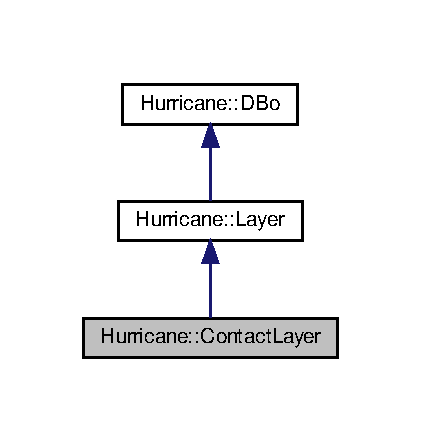
\includegraphics[width=202pt]{classHurricane_1_1ContactLayer__inherit__graph}
\end{center}
\end{figure}
\doxysubsection*{Static Public Member Functions}
\begin{DoxyCompactItemize}
\item 
static \mbox{\hyperlink{classHurricane_1_1ContactLayer}{Contact\+Layer}} $\ast$ \mbox{\hyperlink{classHurricane_1_1ContactLayer_ab5f2e78865e0311fcabf25e1aa94bf09}{create}} (\mbox{\hyperlink{classHurricane_1_1Technology}{Technology}} $\ast$technology, const \mbox{\hyperlink{classHurricane_1_1Name}{Name}} \&name, \mbox{\hyperlink{classHurricane_1_1BasicLayer}{Basic\+Layer}} $\ast$metal\+Layer, \mbox{\hyperlink{classHurricane_1_1BasicLayer}{Basic\+Layer}} $\ast$cut\+Layer, \mbox{\hyperlink{classHurricane_1_1BasicLayer}{Basic\+Layer}} $\ast$active\+Layer, \mbox{\hyperlink{classHurricane_1_1BasicLayer}{Basic\+Layer}} $\ast$diffusion\+Layer, \mbox{\hyperlink{classHurricane_1_1BasicLayer}{Basic\+Layer}} $\ast$well\+Layer)
\end{DoxyCompactItemize}
\doxysubsection*{Additional Inherited Members}


\doxysubsection{Detailed Description}
\mbox{\hyperlink{classHurricane_1_1ContactLayer}{Contact\+Layer}} description ({\bfseries{API}}) 

For a more complete description of the Layers objects, please refer to \mbox{\hyperlink{classHurricane_1_1Layer_secLayerIntro}{Layer Introduction}}.

\mbox{\hyperlink{classHurricane_1_1ContactLayer}{Contact\+Layer}} is a symbolic layer that contains four layers (metal, cut, active, diffusion) plus an optional well layer. Use it to represent a contact from the first metal level toward an active layer.

The accessors functions\+: 
\begin{DoxyItemize}
\item \mbox{\hyperlink{classHurricane_1_1Layer_a5f7c43a29f3dd02a9ebccbcbf91d6727}{Contact\+Layer\+::get\+Top()}} 
\item \mbox{\hyperlink{classHurricane_1_1Layer_a4dab4552a219d2d900ed0b1245dc6580}{Contact\+Layer\+::get\+Bottom()}} 
\item \mbox{\hyperlink{classHurricane_1_1Layer_a69e76c09a56260169c4f5c145a35a47f}{Contact\+Layer\+::get\+Opposite()}} 
\end{DoxyItemize}Have no meaning here.

Only enclosure is used. Extention cap \& extention width are not used. 

\doxysubsection{Member Function Documentation}
\mbox{\Hypertarget{classHurricane_1_1ContactLayer_ab5f2e78865e0311fcabf25e1aa94bf09}\label{classHurricane_1_1ContactLayer_ab5f2e78865e0311fcabf25e1aa94bf09}} 
\index{Hurricane::ContactLayer@{Hurricane::ContactLayer}!create@{create}}
\index{create@{create}!Hurricane::ContactLayer@{Hurricane::ContactLayer}}
\doxysubsubsection{\texorpdfstring{create()}{create()}}
{\footnotesize\ttfamily \mbox{\hyperlink{classHurricane_1_1ContactLayer}{Contact\+Layer}} $\ast$ Hurricane\+::\+Contact\+Layer\+::create (\begin{DoxyParamCaption}\item[{\mbox{\hyperlink{classHurricane_1_1Technology}{Technology}} $\ast$}]{technology,  }\item[{const \mbox{\hyperlink{classHurricane_1_1Name}{Name}} \&}]{name,  }\item[{\mbox{\hyperlink{classHurricane_1_1BasicLayer}{Basic\+Layer}} $\ast$}]{metal\+Layer,  }\item[{\mbox{\hyperlink{classHurricane_1_1BasicLayer}{Basic\+Layer}} $\ast$}]{cut\+Layer,  }\item[{\mbox{\hyperlink{classHurricane_1_1BasicLayer}{Basic\+Layer}} $\ast$}]{active\+Layer,  }\item[{\mbox{\hyperlink{classHurricane_1_1BasicLayer}{Basic\+Layer}} $\ast$}]{diffusion\+Layer,  }\item[{\mbox{\hyperlink{classHurricane_1_1BasicLayer}{Basic\+Layer}} $\ast$}]{well\+Layer }\end{DoxyParamCaption})\hspace{0.3cm}{\ttfamily [static]}}

creates and returns a new contact layer named {\ttfamily $<$name$>$}, composed of metal, cut, active \& diffusion \mbox{\hyperlink{classHurricane_1_1BasicLayer}{Basic\+Layer}} and an optional WELL \mbox{\hyperlink{classHurricane_1_1BasicLayer}{Basic\+Layer}}. A NULL value indicates that no NWELL is used.

\begin{DoxyParagraph}{Caution\+: Throws an exception if the technology is null, if the name is }
empty, if a layer of same name already exists or if we overflow the capacity of the bit field associated to the layer mask. 
\end{DoxyParagraph}


The documentation for this class was generated from the following files\+:\begin{DoxyCompactItemize}
\item 
Contact\+Layer.\+h\item 
Contact\+Layer.\+dox\end{DoxyCompactItemize}

\hypertarget{classHurricane_1_1DataBase}{}\doxysection{Hurricane\+::Data\+Base Class Reference}
\label{classHurricane_1_1DataBase}\index{Hurricane::DataBase@{Hurricane::DataBase}}


The whole \mbox{\hyperlink{classHurricane_1_1DataBase}{Data\+Base}} ({\bfseries{API}}).  




Inheritance diagram for Hurricane\+::Data\+Base\+:\nopagebreak
\begin{figure}[H]
\begin{center}
\leavevmode
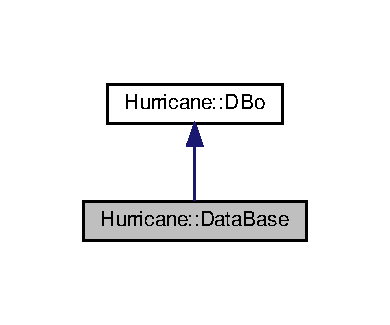
\includegraphics[width=187pt]{classHurricane_1_1DataBase__inherit__graph}
\end{center}
\end{figure}
\doxysubsection*{Public Member Functions}
\begin{DoxyCompactItemize}
\item 
\mbox{\hyperlink{classHurricane_1_1Technology}{Technology}} $\ast$ \mbox{\hyperlink{classHurricane_1_1DataBase_a144480c54b0f9fbda57622ad6767ab8a}{get\+Technology}} () const
\item 
\mbox{\hyperlink{classHurricane_1_1Library}{Library}} $\ast$ \mbox{\hyperlink{classHurricane_1_1DataBase_a4469391a3c5ae82caf090f1bdac4f29b}{get\+Root\+Library}} () const
\end{DoxyCompactItemize}
\doxysubsection*{Static Public Member Functions}
\begin{DoxyCompactItemize}
\item 
static \mbox{\hyperlink{classHurricane_1_1DataBase}{Data\+Base}} $\ast$ \mbox{\hyperlink{classHurricane_1_1DataBase_af0210f9bb13faf06e12eb135eeea9b06}{create}} ()
\item 
static \mbox{\hyperlink{classHurricane_1_1DataBase}{Data\+Base}} $\ast$ \mbox{\hyperlink{classHurricane_1_1DataBase_a53d0b9fcd06b73f3968c8f238f377a88}{get\+DB}} ()
\end{DoxyCompactItemize}


\doxysubsection{Detailed Description}
The whole \mbox{\hyperlink{classHurricane_1_1DataBase}{Data\+Base}} ({\bfseries{API}}). 

The unique purpose of this object is to handle, at any time, directly or indirectly, the whole set of currently allocated objects of the data base.

This is a singleton object, only one can exist at a given time.

The data base must be created explicitely (it is possible to derive a sub-\/type with specific additional attributes, or use properties to store them).

The Database object handles both the \mbox{\hyperlink{classHurricane_1_1Technology}{Technology}} and the root \mbox{\hyperlink{classHurricane_1_1Library}{Library}}.

\begin{DoxyParagraph}{Caution\+: Destroying the Data\+Base object destroys all data base objects.}

\end{DoxyParagraph}


\doxysubsection{Member Function Documentation}
\mbox{\Hypertarget{classHurricane_1_1DataBase_af0210f9bb13faf06e12eb135eeea9b06}\label{classHurricane_1_1DataBase_af0210f9bb13faf06e12eb135eeea9b06}} 
\index{Hurricane::DataBase@{Hurricane::DataBase}!create@{create}}
\index{create@{create}!Hurricane::DataBase@{Hurricane::DataBase}}
\doxysubsubsection{\texorpdfstring{create()}{create()}}
{\footnotesize\ttfamily \mbox{\hyperlink{classHurricane_1_1DataBase}{Data\+Base}} $\ast$ Hurricane\+::\+Data\+Base\+::create (\begin{DoxyParamCaption}{ }\end{DoxyParamCaption})\hspace{0.3cm}{\ttfamily [static]}}

creates and returns a pointer to a new \mbox{\hyperlink{classHurricane_1_1DataBase}{Data\+Base}}.

\begin{DoxyParagraph}{Caution\+: An exception is thrown if a Database already exists.}

\end{DoxyParagraph}
\mbox{\Hypertarget{classHurricane_1_1DataBase_a144480c54b0f9fbda57622ad6767ab8a}\label{classHurricane_1_1DataBase_a144480c54b0f9fbda57622ad6767ab8a}} 
\index{Hurricane::DataBase@{Hurricane::DataBase}!getTechnology@{getTechnology}}
\index{getTechnology@{getTechnology}!Hurricane::DataBase@{Hurricane::DataBase}}
\doxysubsubsection{\texorpdfstring{getTechnology()}{getTechnology()}}
{\footnotesize\ttfamily \mbox{\hyperlink{classHurricane_1_1Technology}{Technology}} $\ast$ Hurricane\+::\+Data\+Base\+::get\+Technology (\begin{DoxyParamCaption}{ }\end{DoxyParamCaption}) const\hspace{0.3cm}{\ttfamily [inline]}}

\begin{DoxyReturn}{Returns}
the \mbox{\hyperlink{classHurricane_1_1Technology}{Technology}} if it exists, else {\ttfamily NULL}. 
\end{DoxyReturn}
\mbox{\Hypertarget{classHurricane_1_1DataBase_a4469391a3c5ae82caf090f1bdac4f29b}\label{classHurricane_1_1DataBase_a4469391a3c5ae82caf090f1bdac4f29b}} 
\index{Hurricane::DataBase@{Hurricane::DataBase}!getRootLibrary@{getRootLibrary}}
\index{getRootLibrary@{getRootLibrary}!Hurricane::DataBase@{Hurricane::DataBase}}
\doxysubsubsection{\texorpdfstring{getRootLibrary()}{getRootLibrary()}}
{\footnotesize\ttfamily \mbox{\hyperlink{classHurricane_1_1Technology}{Technology}} $\ast$ Hurricane\+::\+Data\+Base\+::get\+Root\+Library (\begin{DoxyParamCaption}{ }\end{DoxyParamCaption}) const\hspace{0.3cm}{\ttfamily [inline]}}

\begin{DoxyReturn}{Returns}
the root \mbox{\hyperlink{classHurricane_1_1Library}{Library}} if it exists, else {\ttfamily NULL}. 
\end{DoxyReturn}
\mbox{\Hypertarget{classHurricane_1_1DataBase_a53d0b9fcd06b73f3968c8f238f377a88}\label{classHurricane_1_1DataBase_a53d0b9fcd06b73f3968c8f238f377a88}} 
\index{Hurricane::DataBase@{Hurricane::DataBase}!getDB@{getDB}}
\index{getDB@{getDB}!Hurricane::DataBase@{Hurricane::DataBase}}
\doxysubsubsection{\texorpdfstring{getDB()}{getDB()}}
{\footnotesize\ttfamily \mbox{\hyperlink{classHurricane_1_1DataBase}{Data\+Base}} $\ast$ Hurricane\+::\+Data\+Base\+::get\+DB (\begin{DoxyParamCaption}{ }\end{DoxyParamCaption})\hspace{0.3cm}{\ttfamily [static]}}

This static function returns the current \mbox{\hyperlink{classHurricane_1_1DataBase}{Data\+Base}}, if it has been created and not destroyed, else {\ttfamily NULL}. 

The documentation for this class was generated from the following files\+:\begin{DoxyCompactItemize}
\item 
Data\+Base.\+h\item 
Data\+Base.\+dox\end{DoxyCompactItemize}

\hypertarget{classHurricane_1_1DBo}{}\doxysection{Hurricane\+::DBo Class Reference}
\label{classHurricane_1_1DBo}\index{Hurricane::DBo@{Hurricane::DBo}}


\mbox{\hyperlink{classHurricane_1_1DataBase}{Data\+Base}} object root class ({\bfseries{API}}).  




Inheritance diagram for Hurricane\+::DBo\+:\nopagebreak
\begin{figure}[H]
\begin{center}
\leavevmode
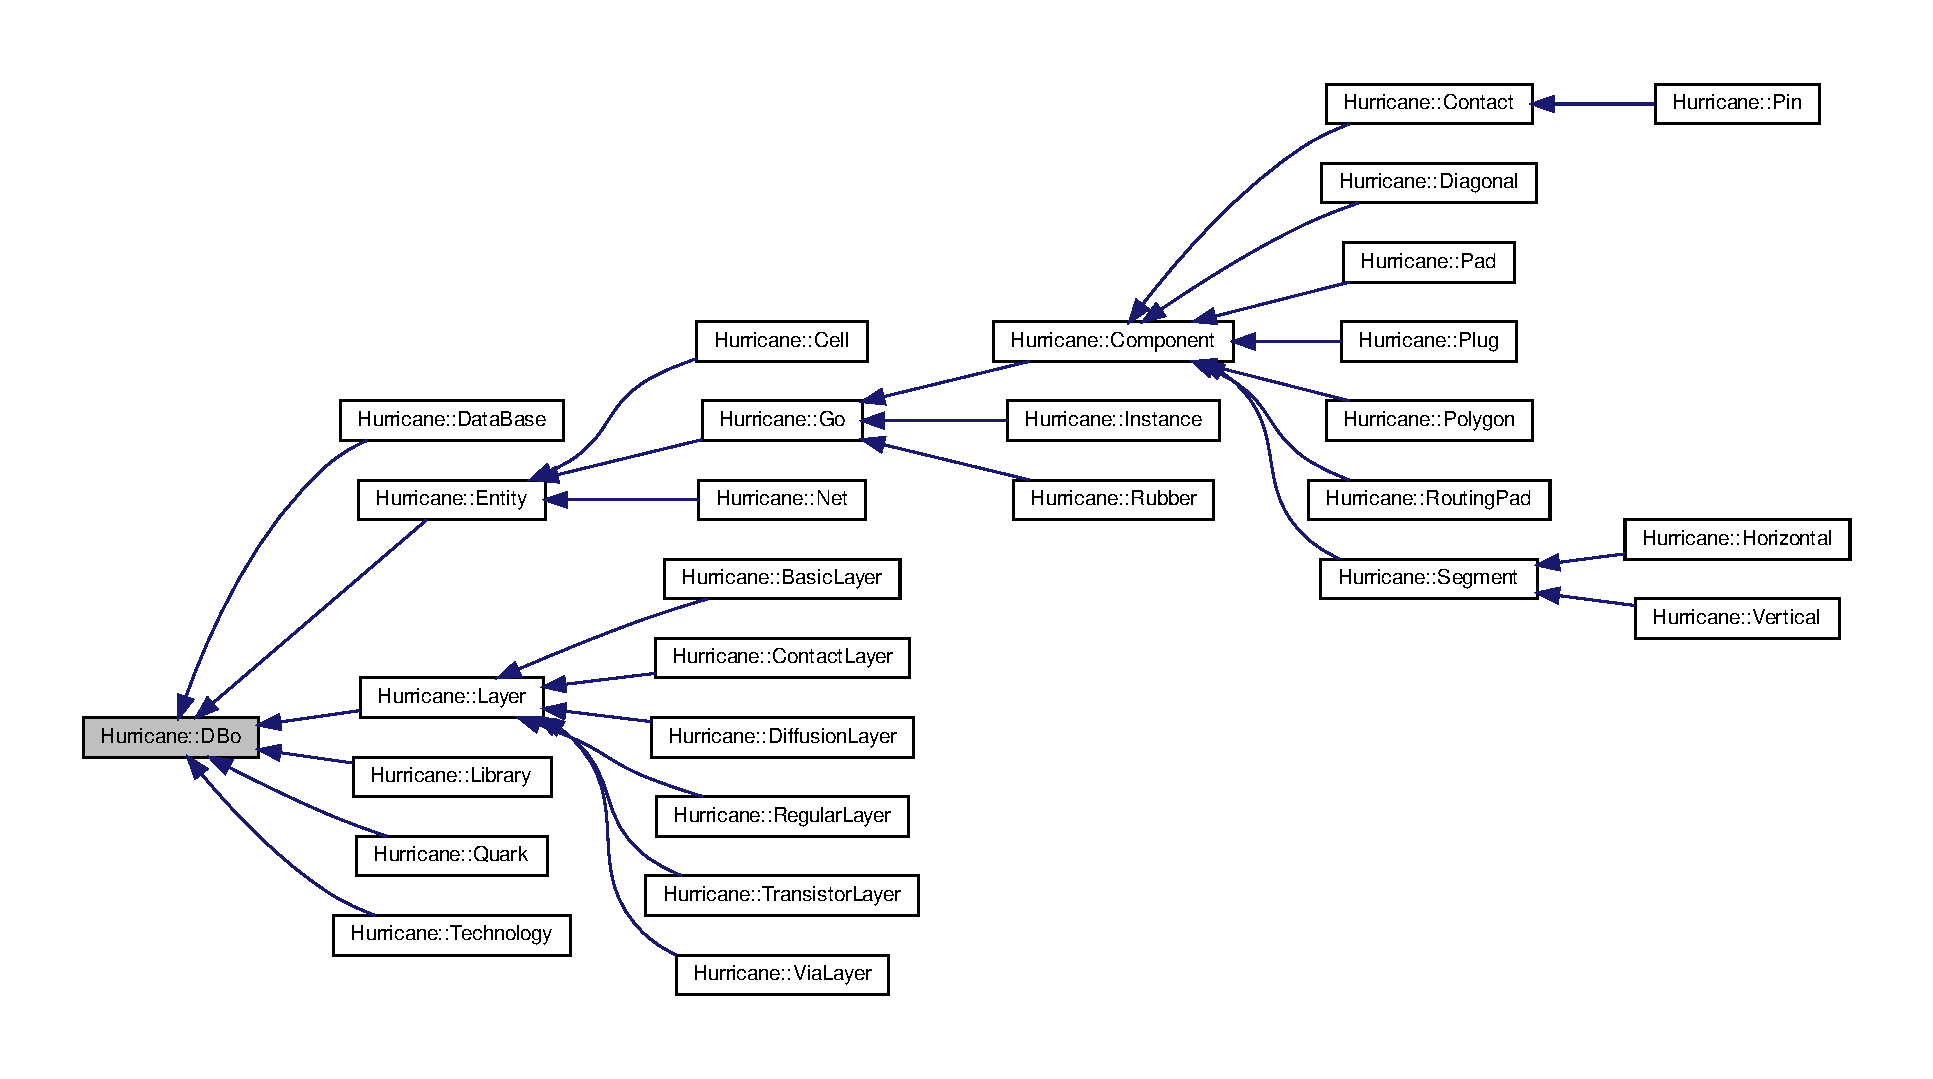
\includegraphics[width=350pt]{classHurricane_1_1DBo__inherit__graph}
\end{center}
\end{figure}
\doxysubsection*{Public Member Functions}
\begin{DoxyCompactItemize}
\item 
virtual void \mbox{\hyperlink{classHurricane_1_1DBo_a67febf5bf9c8b322674648688639728b}{destroy}} ()
\item 
\mbox{\hyperlink{classHurricane_1_1Property}{Property}} $\ast$ \mbox{\hyperlink{classHurricane_1_1DBo_a599f61978df51d1d4c351f6cbd02488d}{get\+Property}} (const \mbox{\hyperlink{classHurricane_1_1Name}{Name}} \&) const
\item 
\mbox{\hyperlink{namespaceHurricane_afd7bca6dad4be54b7c03b0463e6c0004}{Properties}} \mbox{\hyperlink{classHurricane_1_1DBo_aec46894a10e83abb54c495dc4d90f2d3}{get\+Properties}} () const
\item 
bool \mbox{\hyperlink{classHurricane_1_1DBo_a1563f094565030c77592ed82f9a9989b}{has\+Property}} () const
\item 
void \mbox{\hyperlink{classHurricane_1_1DBo_a8979674f11507cb4c7c5251b41ed72d5}{put}} (\mbox{\hyperlink{classHurricane_1_1Property}{Property}} $\ast$)
\item 
void \mbox{\hyperlink{classHurricane_1_1DBo_a7833a1f0b8c704930bdc00861e63cf5e}{remove}} (\mbox{\hyperlink{classHurricane_1_1Property}{Property}} $\ast$)
\item 
void \mbox{\hyperlink{classHurricane_1_1DBo_ac35fbb8303b1a78db5ca0fc831fb6a0c}{remove\+Property}} (const \mbox{\hyperlink{classHurricane_1_1Name}{Name}} \&)
\item 
void \mbox{\hyperlink{classHurricane_1_1DBo_a3e02f3d665cb0b2120df2fdfe9c3df4f}{clear\+Properties}} ()
\end{DoxyCompactItemize}


\doxysubsection{Detailed Description}
\mbox{\hyperlink{classHurricane_1_1DataBase}{Data\+Base}} object root class ({\bfseries{API}}). 

\hypertarget{classHurricane_1_1DBo_sDBoIntro}{}\doxysubsection{Introduction}\label{classHurricane_1_1DBo_sDBoIntro}
All data base objects must be created explicitely by using the provided creation functions and not by calling directly the new operator (which anyway is not provided).

On the same way, they must not be deleted with the delete operator but by calling the destruction function described below.

Those objects can\textquotesingle{}t, either, be duplicated \+: the copy constructor and the assignment operator are not available.

Properties can be attached to those objects (the principles driving the properties management are detailed in the \mbox{\hyperlink{classHurricane_1_1Property}{Property}} class).\hypertarget{classHurricane_1_1DBo_sDBoCreation}{}\doxysubsection{Creation process}\label{classHurricane_1_1DBo_sDBoCreation}
The data base objects are strongly linked between them and some relations can\textquotesingle{}t be set-\/up by the constructors themselves but must be established a posteriori. {\bfseries{Those objects must therefore be built by special functions which take care of that obscure work}}.

Indeed, let us imagine a {\bfseries{\mbox{\hyperlink{classHurricane_1_1Go}{Go}}}} type representing the category of graphic objects and two sub-\/classes {\bfseries{Rectangle}} and {\bfseries{Line}} having specific geometric attributes. For eficiency reasons those {\bfseries{\mbox{\hyperlink{classHurricane_1_1Go}{Go}}}} are stored in a fast access geometric data structure like a {\bfseries{\mbox{\hyperlink{classHurricane_1_1QuadTree}{Quad\+Tree}}}}. It would be ideal that the insertion of the {\bfseries{\mbox{\hyperlink{classHurricane_1_1Go}{Go}}}} within its {\bfseries{\mbox{\hyperlink{classHurricane_1_1QuadTree}{Quad\+Tree}}}} be automatic. This could be done in the {\bfseries{\mbox{\hyperlink{classHurricane_1_1Go}{Go}}}} constructor for instance. But, when this constructor is called upon (by the constructor of sub-\/classes) it is impossible to determine the bounding box of the object because all geometric characteristics are not yet assigned (making the insertion unfeasible).

A possible solution would be to do nothing within the {\bfseries{\mbox{\hyperlink{classHurricane_1_1Go}{Go}}}} constructor and let the work be done by the sub-\/classes constructors wich could call upon the right insertion function. This solution is neither smart nor consistent because an omission can happen. If a sub-\/type of {\bfseries{Line}} is created, the insertion being already done in the {\bfseries{Line}} constructor, it must not be re-\/done for the derived class. Conversely if a new type of {\bfseries{\mbox{\hyperlink{classHurricane_1_1Go}{Go}}}} is created, insertion processing must not be forgotten. Code omissions or duplications are bound to happen and the code is not homogeneous.

Therefore this insertion must be realized by the {\bfseries{\mbox{\hyperlink{classHurricane_1_1Go}{Go}}}}, but a posteriori, that is once the object has been fully built. In order to realize such an operation it must, once all derived classes constructors have been called, call upon a function {\bfseries{\+\_\+post\+Create}} which realizes the additional work and then return the pointer on the new objects (let us recall that all member functions which must not be called directly are prefixed by an underscore).

This process in two steps is realized by the {\bfseries{Create}} function which is provided for each type of instanciable object. The following example shows its implementation for a net \+: 
\begin{DoxyCode}{0}
\DoxyCodeLine{Net* Net::Create(Cell* cell, \textcolor{keyword}{const} Name\& name)}
\DoxyCodeLine{\{}
\DoxyCodeLine{   Net* net = \textcolor{keyword}{new} Net(cell, name);}
\DoxyCodeLine{ }
\DoxyCodeLine{   \textcolor{keywordflow}{if} (!net)}
\DoxyCodeLine{      \textcolor{keywordflow}{throw} Error(\textcolor{stringliteral}{"{}Can't create Net : allocation failed"{}});}
\DoxyCodeLine{ }
\DoxyCodeLine{   net-\/>\_postCreate();}
\DoxyCodeLine{ }
\DoxyCodeLine{   \textcolor{keywordflow}{return} net;}
\DoxyCodeLine{\}}

\end{DoxyCode}


Within this function, the net is created in a first time thanks to the constructor spawn by the new operator. If everything goes right the function {\bfseries{\+\_\+post\+Create}} is called upon the net. This one realizes the additional operations that the constructor couldn\textquotesingle{}t realize and then calls the functions {\bfseries{\+\_\+post\+Create}} upon the base classe. If everything goes right the net is returned, else an exception is thrown if something abnormal or illegal occurs (i.\+e. a net with the same name already exists). For the example of a {\bfseries{Line}} \+: the different called constructors will fully characterize the line, then the {\bfseries{\+\_\+post\+Create}} method on a line will do nothing else than call upon the {\bfseries{\+\_\+post\+Create}} method of the {\bfseries{go}} which will insert the line within the {\bfseries{\mbox{\hyperlink{classHurricane_1_1QuadTree}{Quad\+Tree}}}} (this is now feasible, the line geometry being fully characterized).\hypertarget{classHurricane_1_1DBo_sDBodestroy}{}\doxysubsection{Deletion process}\label{classHurricane_1_1DBo_sDBodestroy}
{\bfseries{The \mbox{\hyperlink{classHurricane_1_1DBo_a67febf5bf9c8b322674648688639728b}{destroy()}} member function \+:}}

Data base ojects can be destroyed only by calling upon this function and not by calling the C++ standard destructor (which indeed is not provided).

A process similar but opposite to the creation process is required. A function {\bfseries{\+\_\+pre\+Destroy}} must be called upon before the effective object destruction. As a matter of fact, if we take again the case of the {\bfseries{Line}} for example, the line must be removed from the {\bfseries{\mbox{\hyperlink{classHurricane_1_1QuadTree}{Quad\+Tree}}}} before the destruction of its geometric characteristics (inverse of the previous phenomenon). Therefore the destroy function is implemented that way \+: 
\begin{DoxyCode}{0}
\DoxyCodeLine{\textcolor{keywordtype}{void} \mbox{\hyperlink{classHurricane_1_1DBo_a67febf5bf9c8b322674648688639728b}{DBo::destroy}}()}
\DoxyCodeLine{\textcolor{comment}{// ***************}}
\DoxyCodeLine{\{}
\DoxyCodeLine{  \_preDestroy();}
\DoxyCodeLine{                }
\DoxyCodeLine{  \textcolor{keyword}{delete} \textcolor{keyword}{this};}
\DoxyCodeLine{\}}

\end{DoxyCode}
\hypertarget{classHurricane_1_1DBo_sDBoExtentions}{}\doxysubsection{Extentions}\label{classHurricane_1_1DBo_sDBoExtentions}
For any new sub-\/type of \mbox{\hyperlink{classHurricane_1_1DBo}{DBo}} you must adhere to the same protocol. That is provide the methods \+\_\+post\+Create and \+\_\+pre\+Destroy calling the methods \+\_\+post\+Create and \+\_\+pre\+Destroy of their base class. Furthermore you must provide when this class is instantiable a creation function (caution \+: only the creation function, if any, must be {\ttfamily public} (and {\ttfamily static}) the others must be {\ttfamily protected}).

Extracted from the .h of a new type of cell. 
\begin{DoxyCode}{0}
\DoxyCodeLine{\textcolor{keyword}{class }MyCell : \textcolor{keyword}{public} Cell \{}
\DoxyCodeLine{  \textcolor{keyword}{public}:  }
\DoxyCodeLine{    \textcolor{keyword}{typedef}  Cell  Inherit;}
\DoxyCodeLine{  \textcolor{keyword}{public}:}
\DoxyCodeLine{    \textcolor{comment}{// User-\/accessible creation method.}}
\DoxyCodeLine{    \textcolor{keyword}{static}  MyCell* Create      (Library* library, \textcolor{keyword}{const} Name\& name);}
\DoxyCodeLine{  \textcolor{keyword}{protected}:}
\DoxyCodeLine{    \textcolor{comment}{// Internally used constructors \& destructors. }}
\DoxyCodeLine{                    MyCell      (Library* library, \textcolor{keyword}{const} Name\& name);}
\DoxyCodeLine{    \textcolor{keyword}{virtual} \textcolor{keywordtype}{void}    \_postCreate ();}
\DoxyCodeLine{    \textcolor{keyword}{virtual} \textcolor{keywordtype}{void}    \_preDestroy ();}
\DoxyCodeLine{\};}

\end{DoxyCode}
 Extracted from the .cpp for this new type of cell. 
\begin{DoxyCode}{0}
\DoxyCodeLine{MyCell::MyCell(Library* library, \textcolor{keyword}{const} Name\&amp; name)}
\DoxyCodeLine{  : Inherit(library, name)}
\DoxyCodeLine{\{ \}}
\DoxyCodeLine{ }
\DoxyCodeLine{}
\DoxyCodeLine{MyCell* MyCell::Create(Library* library, \textcolor{keyword}{const} Name\& name)}
\DoxyCodeLine{\{}
\DoxyCodeLine{  MyCell* myCell = \textcolor{keyword}{new} MyCell(library, name);}
\DoxyCodeLine{ }
\DoxyCodeLine{  \textcolor{keywordflow}{if} (!myCell) \textcolor{keywordflow}{throw} Error(\textcolor{stringliteral}{"{}Can't create MyCell : allocation failed"{}});}
\DoxyCodeLine{ }
\DoxyCodeLine{  myCell-\/>\_postCreate(); \textcolor{comment}{// must not be forgotten!}}
\DoxyCodeLine{ }
\DoxyCodeLine{  \textcolor{keywordflow}{return} myCell;}
\DoxyCodeLine{\}}
\DoxyCodeLine{ }
\DoxyCodeLine{}
\DoxyCodeLine{\textcolor{keywordtype}{void}  MyCell::\_postCreate()}
\DoxyCodeLine{\{}
\DoxyCodeLine{   Inherit::\_postCreate(); \textcolor{comment}{// must not be forgotten!}}
\DoxyCodeLine{ }
\DoxyCodeLine{   \textcolor{comment}{// complete here the post creation}}
\DoxyCodeLine{\}}
\DoxyCodeLine{ }
\DoxyCodeLine{}
\DoxyCodeLine{\textcolor{keywordtype}{void}  MyCell::\_preDestroy()}
\DoxyCodeLine{\{}
\DoxyCodeLine{   Inherit::\_preDestroy(); \textcolor{comment}{// must not be forgotten!}}
\DoxyCodeLine{ }
\DoxyCodeLine{   \textcolor{comment}{// complete here the pre-\/deletion.}}
\DoxyCodeLine{\}}

\end{DoxyCode}


\begin{DoxyRemark}{Remarks}
The destructor, strictly speaking, is not defined because necessary operations are done within the method {\bfseries{\+\_\+pre\+Destroy}}. In the implementation of the class {\bfseries{My\+Cell}} we have only used the type {\bfseries{Inherit}} (and never {\bfseries{\mbox{\hyperlink{classHurricane_1_1Cell}{Cell}}}}). This opens the door to hierarchy changes without affecting the code already written.
\end{DoxyRemark}
\hypertarget{classHurricane_1_1DBo_sDBoRemark}{}\doxysubsection{Remark}\label{classHurricane_1_1DBo_sDBoRemark}
The construction and deletion process of property objects is the same. It is mandatory for any new type of property to adopt the same protocol. 

\doxysubsection{Member Function Documentation}
\mbox{\Hypertarget{classHurricane_1_1DBo_a67febf5bf9c8b322674648688639728b}\label{classHurricane_1_1DBo_a67febf5bf9c8b322674648688639728b}} 
\index{Hurricane::DBo@{Hurricane::DBo}!destroy@{destroy}}
\index{destroy@{destroy}!Hurricane::DBo@{Hurricane::DBo}}
\doxysubsubsection{\texorpdfstring{destroy()}{destroy()}}
{\footnotesize\ttfamily void Hurricane\+::\+DBo\+::destroy (\begin{DoxyParamCaption}{ }\end{DoxyParamCaption})\hspace{0.3cm}{\ttfamily [virtual]}}

The legal method to delete any \mbox{\hyperlink{classHurricane_1_1DBo}{DBo}} object (see \mbox{\hyperlink{classHurricane_1_1DBo_sDBodestroy}{Deletion process}}). \mbox{\Hypertarget{classHurricane_1_1DBo_a599f61978df51d1d4c351f6cbd02488d}\label{classHurricane_1_1DBo_a599f61978df51d1d4c351f6cbd02488d}} 
\index{Hurricane::DBo@{Hurricane::DBo}!getProperty@{getProperty}}
\index{getProperty@{getProperty}!Hurricane::DBo@{Hurricane::DBo}}
\doxysubsubsection{\texorpdfstring{getProperty()}{getProperty()}}
{\footnotesize\ttfamily \mbox{\hyperlink{classHurricane_1_1Property}{Property}} $\ast$ Hurricane\+::\+DBo\+::get\+Property (\begin{DoxyParamCaption}\item[{const \mbox{\hyperlink{classHurricane_1_1Name}{Name}} \&}]{name }\end{DoxyParamCaption}) const}


\begin{DoxyParams}{Parameters}
{\em name} & \mbox{\hyperlink{classHurricane_1_1Name}{Name}} of the \mbox{\hyperlink{classHurricane_1_1Property}{Property}} to return. \\
\hline
\end{DoxyParams}
\begin{DoxyReturn}{Returns}
The property of \mbox{\hyperlink{classHurricane_1_1Name}{Name}} {\itshape name} attached to the object, if it exists, else {\ttfamily NULL}.
\end{DoxyReturn}
\begin{DoxyRemark}{Remarks}
When writting what follows \+: 
\begin{DoxyCode}{0}
\DoxyCodeLine{forEach(DBo*, idbo, dbos) \{}
\DoxyCodeLine{  Property* \textcolor{keyword}{property} = idbo-\/>getProperty(\textcolor{stringliteral}{"{}width"{}});}
\DoxyCodeLine{  \textcolor{keywordflow}{if} (property) \{}
\DoxyCodeLine{    \textcolor{comment}{// do something}}
\DoxyCodeLine{  \}}
\DoxyCodeLine{\}}

\end{DoxyCode}

\end{DoxyRemark}
There is construction of a name (from a character string) for each visited dbo in order to find the property. It\textquotesingle{}s more efficient to write \+: 
\begin{DoxyCode}{0}
\DoxyCodeLine{Name width = \textcolor{stringliteral}{"{}width"{}};}
\DoxyCodeLine{forEach(DBo*, idbo, dbos) \{}
\DoxyCodeLine{  Property* \textcolor{keyword}{property} = idbo-\/>getProperty(width);}
\DoxyCodeLine{  \textcolor{keywordflow}{if} (property) \{}
\DoxyCodeLine{    \textcolor{comment}{// do something}}
\DoxyCodeLine{  \}}
\DoxyCodeLine{\}}

\end{DoxyCode}
 Or still better \+: 
\begin{DoxyCode}{0}
\DoxyCodeLine{\textcolor{keyword}{static} Name WIDTH = \textcolor{stringliteral}{"{}width"{}};}
\DoxyCodeLine{forEach(DBo*, idbo, dbos) \{}
\DoxyCodeLine{  Property* \textcolor{keyword}{property} = idbo-\/>getProperty(WIDTH);}
\DoxyCodeLine{  \textcolor{keywordflow}{if} (property) \{}
\DoxyCodeLine{    \textcolor{comment}{// do something}}
\DoxyCodeLine{  \}}
\DoxyCodeLine{\}}

\end{DoxyCode}
 This remark applies each time you handle names. \mbox{\Hypertarget{classHurricane_1_1DBo_aec46894a10e83abb54c495dc4d90f2d3}\label{classHurricane_1_1DBo_aec46894a10e83abb54c495dc4d90f2d3}} 
\index{Hurricane::DBo@{Hurricane::DBo}!getProperties@{getProperties}}
\index{getProperties@{getProperties}!Hurricane::DBo@{Hurricane::DBo}}
\doxysubsubsection{\texorpdfstring{getProperties()}{getProperties()}}
{\footnotesize\ttfamily Propertes Hurricane\+::\+DBo\+::get\+Properties (\begin{DoxyParamCaption}{ }\end{DoxyParamCaption}) const}

\begin{DoxyReturn}{Returns}
The property \mbox{\hyperlink{classHurricane_1_1Collection}{Collection}} associated to the object (possibly empty). 
\end{DoxyReturn}
\mbox{\Hypertarget{classHurricane_1_1DBo_a1563f094565030c77592ed82f9a9989b}\label{classHurricane_1_1DBo_a1563f094565030c77592ed82f9a9989b}} 
\index{Hurricane::DBo@{Hurricane::DBo}!hasProperty@{hasProperty}}
\index{hasProperty@{hasProperty}!Hurricane::DBo@{Hurricane::DBo}}
\doxysubsubsection{\texorpdfstring{hasProperty()}{hasProperty()}}
{\footnotesize\ttfamily bool Hurricane\+::\+DBo\+::has\+Property (\begin{DoxyParamCaption}{ }\end{DoxyParamCaption}) const\hspace{0.3cm}{\ttfamily [inline]}}

\begin{DoxyReturn}{Returns}
{\bfseries{true}} if the object has at least a property, else {\bfseries{false}}. 
\end{DoxyReturn}
\mbox{\Hypertarget{classHurricane_1_1DBo_a8979674f11507cb4c7c5251b41ed72d5}\label{classHurricane_1_1DBo_a8979674f11507cb4c7c5251b41ed72d5}} 
\index{Hurricane::DBo@{Hurricane::DBo}!put@{put}}
\index{put@{put}!Hurricane::DBo@{Hurricane::DBo}}
\doxysubsubsection{\texorpdfstring{put()}{put()}}
{\footnotesize\ttfamily void Hurricane\+::\+DBo\+::put (\begin{DoxyParamCaption}\item[{\mbox{\hyperlink{classHurricane_1_1Property}{Property}} $\ast$}]{property }\end{DoxyParamCaption})}

Adds the \mbox{\hyperlink{classHurricane_1_1Property}{Property}} {\itshape property} to the set of object properties. Properties being named, if an other one already exists in the set, with the same name, this last will be in a first step removed from the set.

\begin{DoxyRemark}{Remarks}
Does nothing if the \mbox{\hyperlink{classHurricane_1_1Property}{Property}} object is already attached to the object.
\end{DoxyRemark}
\begin{DoxyParagraph}{Caution\+: An exception is thrown if the Property pointer is {\ttfamily NULL}.}

\end{DoxyParagraph}
\mbox{\Hypertarget{classHurricane_1_1DBo_a7833a1f0b8c704930bdc00861e63cf5e}\label{classHurricane_1_1DBo_a7833a1f0b8c704930bdc00861e63cf5e}} 
\index{Hurricane::DBo@{Hurricane::DBo}!remove@{remove}}
\index{remove@{remove}!Hurricane::DBo@{Hurricane::DBo}}
\doxysubsubsection{\texorpdfstring{remove()}{remove()}}
{\footnotesize\ttfamily void Hurricane\+::\+DBo\+::remove (\begin{DoxyParamCaption}\item[{\mbox{\hyperlink{classHurricane_1_1Property}{Property}} $\ast$}]{property }\end{DoxyParamCaption})}

removes the property {\itshape property} from the set of object properties.

\begin{DoxyRemark}{Remarks}
Does nothing if the \mbox{\hyperlink{classHurricane_1_1Property}{Property}} object is not attached to the object.
\end{DoxyRemark}
\begin{DoxyParagraph}{Caution\+: An exception is thrown if the Property pointer is {\ttfamily NULL}.}

\end{DoxyParagraph}
\mbox{\Hypertarget{classHurricane_1_1DBo_ac35fbb8303b1a78db5ca0fc831fb6a0c}\label{classHurricane_1_1DBo_ac35fbb8303b1a78db5ca0fc831fb6a0c}} 
\index{Hurricane::DBo@{Hurricane::DBo}!removeProperty@{removeProperty}}
\index{removeProperty@{removeProperty}!Hurricane::DBo@{Hurricane::DBo}}
\doxysubsubsection{\texorpdfstring{removeProperty()}{removeProperty()}}
{\footnotesize\ttfamily void Hurricane\+::\+DBo\+::remove\+Property (\begin{DoxyParamCaption}\item[{const \mbox{\hyperlink{classHurricane_1_1Name}{Name}} \&}]{name }\end{DoxyParamCaption})}

removes the property of name {\itshape name} if it exists. \mbox{\Hypertarget{classHurricane_1_1DBo_a3e02f3d665cb0b2120df2fdfe9c3df4f}\label{classHurricane_1_1DBo_a3e02f3d665cb0b2120df2fdfe9c3df4f}} 
\index{Hurricane::DBo@{Hurricane::DBo}!clearProperties@{clearProperties}}
\index{clearProperties@{clearProperties}!Hurricane::DBo@{Hurricane::DBo}}
\doxysubsubsection{\texorpdfstring{clearProperties()}{clearProperties()}}
{\footnotesize\ttfamily void Hurricane\+::\+DBo\+::clear\+Properties (\begin{DoxyParamCaption}{ }\end{DoxyParamCaption})}

removes all properties attached to this object. 

The documentation for this class was generated from the following files\+:\begin{DoxyCompactItemize}
\item 
DBo.\+h\item 
DBo.\+dox\end{DoxyCompactItemize}

\hypertarget{classHurricane_1_1DbU}{}\doxysection{Hurricane\+::DbU Class Reference}
\label{classHurricane_1_1DbU}\index{Hurricane::DbU@{Hurricane::DbU}}


\mbox{\hyperlink{classHurricane_1_1DataBase}{Data\+Base}} Unit managment ({\bfseries{API}}).  


\doxysubsection*{Public Types}
\begin{DoxyCompactItemize}
\item 
enum \mbox{\hyperlink{classHurricane_1_1DbU_a6af6a5b8d113a661fea65b2bcb8b25c4}{String\+Mode}} \{ \newline
\mbox{\hyperlink{classHurricane_1_1DbU_a6af6a5b8d113a661fea65b2bcb8b25c4a1b91af5faf467afcb73dec10bc54f233}{Db}} = (1$<$$<$0)
, \newline
\mbox{\hyperlink{classHurricane_1_1DbU_a6af6a5b8d113a661fea65b2bcb8b25c4ac6b6574b2ef79ee4e44c6c00fe757c7c}{Grid}} = (1$<$$<$1)
, \newline
\mbox{\hyperlink{classHurricane_1_1DbU_a6af6a5b8d113a661fea65b2bcb8b25c4a16f8df0900c42b001f0a91475a1b93f8}{Symbolic}} = (1$<$$<$2)
, \newline
{\bfseries Physical} = (1$<$$<$3)
, \newline
{\bfseries Smart\+Truncate} = (1$<$$<$4)
 \}
\item 
typedef std\+::int64\+\_\+t \mbox{\hyperlink{classHurricane_1_1DbU_a4fbfa3e8c89347af76c9628ea06c4146}{Unit}}
\end{DoxyCompactItemize}
\doxysubsection*{Static Public Member Functions}
\begin{DoxyCompactItemize}
\item 
static \mbox{\hyperlink{classHurricane_1_1DbU_a4fbfa3e8c89347af76c9628ea06c4146}{Unit}} \mbox{\hyperlink{classHurricane_1_1DbU_aec69d65ec1651c2feea24c5931f4580b}{from\+Db}} (\mbox{\hyperlink{classHurricane_1_1DbU_a4fbfa3e8c89347af76c9628ea06c4146}{Unit}} value)
\item 
static \mbox{\hyperlink{classHurricane_1_1DbU_a4fbfa3e8c89347af76c9628ea06c4146}{Unit}} \mbox{\hyperlink{classHurricane_1_1DbU_a367e1d1b5ac1df076745550cba8a83c1}{from\+Grid}} (double value)
\item 
static \mbox{\hyperlink{classHurricane_1_1DbU_a4fbfa3e8c89347af76c9628ea06c4146}{Unit}} \mbox{\hyperlink{classHurricane_1_1DbU_a4b570755b19ea9ff0f2f258a221bd935}{from\+Lambda}} (double value)
\item 
static \mbox{\hyperlink{classHurricane_1_1DbU_a4fbfa3e8c89347af76c9628ea06c4146}{Unit}} \mbox{\hyperlink{classHurricane_1_1DbU_a11d4dbd9134a19bda35cbacde1cb2769}{from\+Physical}} (double value, \mbox{\hyperlink{classHurricane_1_1DbU_a50b5785bf4d75026c4c112caec3040a7}{Unit\+Power}} p)
\item 
static unsigned int \mbox{\hyperlink{classHurricane_1_1DbU_a6169efbdd9b3d54a0bd8467c8f957fda}{get\+Precision}} ()
\item 
static unsigned int \mbox{\hyperlink{classHurricane_1_1DbU_a8756c9f0a32af5f601cd150e73b02c03}{get\+Maximal\+Precision}} ()
\item 
static double \mbox{\hyperlink{classHurricane_1_1DbU_a120a60b09b344d01c583567a1e489d9e}{get\+Resolution}} ()
\item 
static void \mbox{\hyperlink{classHurricane_1_1DbU_ace9a8644e7e80dcaed2a8a95deeb1622}{set\+Precision}} (unsigned int precision, unsigned int flags=No\+Flags)
\item 
static void \mbox{\hyperlink{classHurricane_1_1DbU_ac93f9ba2a09105227e34bd05bcb1500c}{set\+Grids\+Per\+Lambda}} (double grids\+Per\+Lambda, unsigned int flags=No\+Flags)
\item 
static double \mbox{\hyperlink{classHurricane_1_1DbU_a9a0359adbfafc356326f5c6adf57ff04}{get\+Grids\+Per\+Lambda}} ()
\item 
static \mbox{\hyperlink{classHurricane_1_1DbU_a4fbfa3e8c89347af76c9628ea06c4146}{Db\+U\+::\+Unit}} \mbox{\hyperlink{classHurricane_1_1DbU_a09e46fcca6aaca94851adfa196e10170}{get\+Real\+Snap\+Grid\+Step}} ()
\item 
static \mbox{\hyperlink{classHurricane_1_1DbU_a4fbfa3e8c89347af76c9628ea06c4146}{Db\+U\+::\+Unit}} \mbox{\hyperlink{classHurricane_1_1DbU_a8746e486f153aa37ee469c1604eba5c0}{get\+On\+Real\+Snap\+Grid}} (\mbox{\hyperlink{classHurricane_1_1DbU_a4fbfa3e8c89347af76c9628ea06c4146}{Db\+U\+::\+Unit}} u, \mbox{\hyperlink{classHurricane_1_1DbU_a1082168d6f9956ebba22ab8bbec21637}{Snap\+Mode}} mode=\mbox{\hyperlink{classHurricane_1_1DbU_a1082168d6f9956ebba22ab8bbec21637a65e6f47eb16779b8974a80d6145a2db5}{Nearest}})
\item 
static void \mbox{\hyperlink{classHurricane_1_1DbU_a202cc3aa3364c2224647a29dde047fae}{set\+Real\+Snap\+Grid\+Step}} (\mbox{\hyperlink{classHurricane_1_1DbU_a4fbfa3e8c89347af76c9628ea06c4146}{Db\+U\+::\+Unit}} step)
\item 
static \mbox{\hyperlink{classHurricane_1_1DbU_a4fbfa3e8c89347af76c9628ea06c4146}{Db\+U\+::\+Unit}} \mbox{\hyperlink{classHurricane_1_1DbU_a687a9134729b107c42fb7f69596c4c3b}{get\+Symbolic\+Snap\+Grid\+Step}} ()
\item 
static \mbox{\hyperlink{classHurricane_1_1DbU_a4fbfa3e8c89347af76c9628ea06c4146}{Db\+U\+::\+Unit}} \mbox{\hyperlink{classHurricane_1_1DbU_ad1b0c0f3680093cf5a63d901312c925d}{get\+On\+Symbolic\+Snap\+Grid}} (\mbox{\hyperlink{classHurricane_1_1DbU_a4fbfa3e8c89347af76c9628ea06c4146}{Db\+U\+::\+Unit}} u, \mbox{\hyperlink{classHurricane_1_1DbU_a1082168d6f9956ebba22ab8bbec21637}{Snap\+Mode}} mode=\mbox{\hyperlink{classHurricane_1_1DbU_a1082168d6f9956ebba22ab8bbec21637a65e6f47eb16779b8974a80d6145a2db5}{Nearest}})
\item 
static void \mbox{\hyperlink{classHurricane_1_1DbU_a9ccd423c8f268ef54770f4663e6c9304}{set\+Symbolic\+Snap\+Grid\+Step}} (\mbox{\hyperlink{classHurricane_1_1DbU_a4fbfa3e8c89347af76c9628ea06c4146}{Db\+U\+::\+Unit}} step)
\item 
static \mbox{\hyperlink{classHurricane_1_1DbU_a4fbfa3e8c89347af76c9628ea06c4146}{Db\+U\+::\+Unit}} \mbox{\hyperlink{classHurricane_1_1DbU_a87323d9038656dceabffc37d45de408a}{get\+On\+Custom\+Grid}} (\mbox{\hyperlink{classHurricane_1_1DbU_a4fbfa3e8c89347af76c9628ea06c4146}{Db\+U\+::\+Unit}} u, \mbox{\hyperlink{classHurricane_1_1DbU_a4fbfa3e8c89347af76c9628ea06c4146}{Db\+U\+::\+Unit}} step, \mbox{\hyperlink{classHurricane_1_1DbU_a1082168d6f9956ebba22ab8bbec21637}{Snap\+Mode}} mode=\mbox{\hyperlink{classHurricane_1_1DbU_a1082168d6f9956ebba22ab8bbec21637a65e6f47eb16779b8974a80d6145a2db5}{Nearest}})
\item 
static \mbox{\hyperlink{classHurricane_1_1DbU_a4fbfa3e8c89347af76c9628ea06c4146}{Db\+U\+::\+Unit}} \mbox{\hyperlink{classHurricane_1_1DbU_a9419025221579f4277475c65655be3dc}{get\+On\+Physical\+Grid}} (\mbox{\hyperlink{classHurricane_1_1DbU_a4fbfa3e8c89347af76c9628ea06c4146}{Db\+U\+::\+Unit}} u, \mbox{\hyperlink{classHurricane_1_1DbU_a1082168d6f9956ebba22ab8bbec21637}{Snap\+Mode}} mode=\mbox{\hyperlink{classHurricane_1_1DbU_a1082168d6f9956ebba22ab8bbec21637a8ce92cf7ff7627c46baf85612f9ad847}{Superior}})
\item 
static \mbox{\hyperlink{classHurricane_1_1DbU_a4fbfa3e8c89347af76c9628ea06c4146}{Unit}} \mbox{\hyperlink{classHurricane_1_1DbU_aec07c6e7ae2a2a6f54e2a16b32c8bf26}{to\+Db}} (\mbox{\hyperlink{classHurricane_1_1DbU_a4fbfa3e8c89347af76c9628ea06c4146}{Unit}} u)
\item 
static double \mbox{\hyperlink{classHurricane_1_1DbU_a318d673386c9424e07c12efd598c730d}{to\+Grid}} (\mbox{\hyperlink{classHurricane_1_1DbU_a4fbfa3e8c89347af76c9628ea06c4146}{Unit}} u)
\item 
static double \mbox{\hyperlink{classHurricane_1_1DbU_a4923a9a443871282ad7d331be2a2a5d4}{to\+Lambda}} (\mbox{\hyperlink{classHurricane_1_1DbU_a4fbfa3e8c89347af76c9628ea06c4146}{Unit}} u)
\item 
static double \mbox{\hyperlink{classHurricane_1_1DbU_ab901e9d5c12e878728178f113def6c45}{to\+Physical}} (\mbox{\hyperlink{classHurricane_1_1DbU_a4fbfa3e8c89347af76c9628ea06c4146}{Unit}} u, \mbox{\hyperlink{classHurricane_1_1DbU_a50b5785bf4d75026c4c112caec3040a7}{Unit\+Power}} p)
\item 
static string \mbox{\hyperlink{classHurricane_1_1DbU_adc9c1a06b4296dbddcf711077113f4bd}{get\+Value\+String}} (\mbox{\hyperlink{classHurricane_1_1DbU_a4fbfa3e8c89347af76c9628ea06c4146}{Unit}} u, int mode=Smart\+Truncate)
\item 
static void \mbox{\hyperlink{classHurricane_1_1DbU_a89ab8f8326c54113336086663ecf1d25}{set\+String\+Mode}} (unsigned int mode, \mbox{\hyperlink{classHurricane_1_1DbU_a50b5785bf4d75026c4c112caec3040a7}{Unit\+Power}} p=\mbox{\hyperlink{classHurricane_1_1DbU_a50b5785bf4d75026c4c112caec3040a7a03e5923be5810db830626f2ca26319d6}{Nano}})
\end{DoxyCompactItemize}
\doxysubsection*{Obsoleteds}
\label{_amgrpf05125b8b6a468721054b36b1a1cfd62}%
 Due to their somewhat unclear naming convention, those functions have been renamed by the {\itshape to} / {\itshape from} variants. \begin{DoxyCompactItemize}
\item 
enum \mbox{\hyperlink{classHurricane_1_1DbU_a50b5785bf4d75026c4c112caec3040a7}{Unit\+Power}} \{ \newline
\mbox{\hyperlink{classHurricane_1_1DbU_a50b5785bf4d75026c4c112caec3040a7a3cf34ad82faf73a9b48dcb3a621d0557}{Pico}} = 1
, \newline
\mbox{\hyperlink{classHurricane_1_1DbU_a50b5785bf4d75026c4c112caec3040a7a03e5923be5810db830626f2ca26319d6}{Nano}}
, \newline
\mbox{\hyperlink{classHurricane_1_1DbU_a50b5785bf4d75026c4c112caec3040a7aa0481a3398a6cbb0a68a523146f0a7fb}{Micro}}
, \newline
\mbox{\hyperlink{classHurricane_1_1DbU_a50b5785bf4d75026c4c112caec3040a7aac2973886c68f16ee68a192154ea65be}{Milli}}
, \newline
\mbox{\hyperlink{classHurricane_1_1DbU_a50b5785bf4d75026c4c112caec3040a7ac5c524bb7247124f3dce7d1dbdc7d2c6}{Unity}}
, \newline
\mbox{\hyperlink{classHurricane_1_1DbU_a50b5785bf4d75026c4c112caec3040a7a7853e18601786b5c51a1bc9cfaf8bb74}{Kilo}}
 \}
\item 
enum \mbox{\hyperlink{classHurricane_1_1DbU_a1082168d6f9956ebba22ab8bbec21637}{Snap\+Mode}} \{ \newline
\mbox{\hyperlink{classHurricane_1_1DbU_a1082168d6f9956ebba22ab8bbec21637a888eae532f84c3f19b024e1830ef8cb3}{Inferior}} = 1
, \newline
\mbox{\hyperlink{classHurricane_1_1DbU_a1082168d6f9956ebba22ab8bbec21637a8ce92cf7ff7627c46baf85612f9ad847}{Superior}} = 2
, \newline
\mbox{\hyperlink{classHurricane_1_1DbU_a1082168d6f9956ebba22ab8bbec21637a65e6f47eb16779b8974a80d6145a2db5}{Nearest}} = 4
 \}
\item 
static \mbox{\hyperlink{classHurricane_1_1DbU_a4fbfa3e8c89347af76c9628ea06c4146}{Unit}} \mbox{\hyperlink{classHurricane_1_1DbU_acd77957381fb93fc4203bdca215e0b48}{db}} (\mbox{\hyperlink{classHurricane_1_1DbU_a4fbfa3e8c89347af76c9628ea06c4146}{Unit}} value)
\item 
static \mbox{\hyperlink{classHurricane_1_1DbU_a4fbfa3e8c89347af76c9628ea06c4146}{Unit}} \mbox{\hyperlink{classHurricane_1_1DbU_a1d4bac6e3b68c8cd44b345de3b425753}{grid}} (double value)
\item 
static \mbox{\hyperlink{classHurricane_1_1DbU_a4fbfa3e8c89347af76c9628ea06c4146}{Unit}} \mbox{\hyperlink{classHurricane_1_1DbU_aa1ba98acc939ff1c370c18544a5e0dce}{lambda}} (double value)
\item 
static \mbox{\hyperlink{classHurricane_1_1DbU_a4fbfa3e8c89347af76c9628ea06c4146}{Unit}} \mbox{\hyperlink{classHurricane_1_1DbU_a4233772b1b3e68f3ec723c7509ea87ff}{get\+Db}} (\mbox{\hyperlink{classHurricane_1_1DbU_a4fbfa3e8c89347af76c9628ea06c4146}{Unit}} u)
\item 
static double \mbox{\hyperlink{classHurricane_1_1DbU_ad4485d0d7b5fd7ae87b32f165155c0a2}{get\+Grid}} (\mbox{\hyperlink{classHurricane_1_1DbU_a4fbfa3e8c89347af76c9628ea06c4146}{Unit}} u)
\item 
static double \mbox{\hyperlink{classHurricane_1_1DbU_adea6b9a6e84243f70f3a5e2725b2c6d8}{get\+Lambda}} (\mbox{\hyperlink{classHurricane_1_1DbU_a4fbfa3e8c89347af76c9628ea06c4146}{Unit}} u)
\end{DoxyCompactItemize}


\doxysubsection{Detailed Description}
\mbox{\hyperlink{classHurricane_1_1DataBase}{Data\+Base}} Unit managment ({\bfseries{API}}). 

{\bfseries{Explanations about this class are here \mbox{\hyperlink{group__DbUGroup}{Db\+U/\+Unit description}}.}} 

\doxysubsection{Member Typedef Documentation}
\mbox{\Hypertarget{classHurricane_1_1DbU_a4fbfa3e8c89347af76c9628ea06c4146}\label{classHurricane_1_1DbU_a4fbfa3e8c89347af76c9628ea06c4146}} 
\index{Hurricane::DbU@{Hurricane::DbU}!Unit@{Unit}}
\index{Unit@{Unit}!Hurricane::DbU@{Hurricane::DbU}}
\doxysubsubsection{\texorpdfstring{Unit}{Unit}}
{\footnotesize\ttfamily long \mbox{\hyperlink{classHurricane_1_1DbU_a4fbfa3e8c89347af76c9628ea06c4146}{Hurricane\+::\+Db\+U\+::\+Unit}}}

The working \mbox{\hyperlink{classHurricane_1_1DataBase}{Data\+Base}} type for storing dimensions. 

\doxysubsection{Member Enumeration Documentation}
\mbox{\Hypertarget{classHurricane_1_1DbU_a50b5785bf4d75026c4c112caec3040a7}\label{classHurricane_1_1DbU_a50b5785bf4d75026c4c112caec3040a7}} 
\index{Hurricane::DbU@{Hurricane::DbU}!UnitPower@{UnitPower}}
\index{UnitPower@{UnitPower}!Hurricane::DbU@{Hurricane::DbU}}
\doxysubsubsection{\texorpdfstring{UnitPower}{UnitPower}}
{\footnotesize\ttfamily enum \mbox{\hyperlink{classHurricane_1_1DbU_a50b5785bf4d75026c4c112caec3040a7}{Hurricane\+::\+Db\+U\+::\+Unit\+Power}}}

This enumeration defines the power applicable to physical units. \begin{DoxyEnumFields}{Enumerator}
\raisebox{\heightof{T}}[0pt][0pt]{\index{Pico@{Pico}!Hurricane::DbU@{Hurricane::DbU}}\index{Hurricane::DbU@{Hurricane::DbU}!Pico@{Pico}}}\mbox{\Hypertarget{classHurricane_1_1DbU_a50b5785bf4d75026c4c112caec3040a7a3cf34ad82faf73a9b48dcb3a621d0557}\label{classHurricane_1_1DbU_a50b5785bf4d75026c4c112caec3040a7a3cf34ad82faf73a9b48dcb3a621d0557}} 
Pico&10e-\/12 \\
\hline

\raisebox{\heightof{T}}[0pt][0pt]{\index{Nano@{Nano}!Hurricane::DbU@{Hurricane::DbU}}\index{Hurricane::DbU@{Hurricane::DbU}!Nano@{Nano}}}\mbox{\Hypertarget{classHurricane_1_1DbU_a50b5785bf4d75026c4c112caec3040a7a03e5923be5810db830626f2ca26319d6}\label{classHurricane_1_1DbU_a50b5785bf4d75026c4c112caec3040a7a03e5923be5810db830626f2ca26319d6}} 
Nano&10e-\/9 \\
\hline

\raisebox{\heightof{T}}[0pt][0pt]{\index{Micro@{Micro}!Hurricane::DbU@{Hurricane::DbU}}\index{Hurricane::DbU@{Hurricane::DbU}!Micro@{Micro}}}\mbox{\Hypertarget{classHurricane_1_1DbU_a50b5785bf4d75026c4c112caec3040a7aa0481a3398a6cbb0a68a523146f0a7fb}\label{classHurricane_1_1DbU_a50b5785bf4d75026c4c112caec3040a7aa0481a3398a6cbb0a68a523146f0a7fb}} 
Micro&10e-\/6 \\
\hline

\raisebox{\heightof{T}}[0pt][0pt]{\index{Milli@{Milli}!Hurricane::DbU@{Hurricane::DbU}}\index{Hurricane::DbU@{Hurricane::DbU}!Milli@{Milli}}}\mbox{\Hypertarget{classHurricane_1_1DbU_a50b5785bf4d75026c4c112caec3040a7aac2973886c68f16ee68a192154ea65be}\label{classHurricane_1_1DbU_a50b5785bf4d75026c4c112caec3040a7aac2973886c68f16ee68a192154ea65be}} 
Milli&10e-\/3 \\
\hline

\raisebox{\heightof{T}}[0pt][0pt]{\index{Unity@{Unity}!Hurricane::DbU@{Hurricane::DbU}}\index{Hurricane::DbU@{Hurricane::DbU}!Unity@{Unity}}}\mbox{\Hypertarget{classHurricane_1_1DbU_a50b5785bf4d75026c4c112caec3040a7ac5c524bb7247124f3dce7d1dbdc7d2c6}\label{classHurricane_1_1DbU_a50b5785bf4d75026c4c112caec3040a7ac5c524bb7247124f3dce7d1dbdc7d2c6}} 
Unity&1 \\
\hline

\raisebox{\heightof{T}}[0pt][0pt]{\index{Kilo@{Kilo}!Hurricane::DbU@{Hurricane::DbU}}\index{Hurricane::DbU@{Hurricane::DbU}!Kilo@{Kilo}}}\mbox{\Hypertarget{classHurricane_1_1DbU_a50b5785bf4d75026c4c112caec3040a7a7853e18601786b5c51a1bc9cfaf8bb74}\label{classHurricane_1_1DbU_a50b5785bf4d75026c4c112caec3040a7a7853e18601786b5c51a1bc9cfaf8bb74}} 
Kilo&10e+3 \\
\hline

\end{DoxyEnumFields}
\mbox{\Hypertarget{classHurricane_1_1DbU_a6af6a5b8d113a661fea65b2bcb8b25c4}\label{classHurricane_1_1DbU_a6af6a5b8d113a661fea65b2bcb8b25c4}} 
\index{Hurricane::DbU@{Hurricane::DbU}!StringMode@{StringMode}}
\index{StringMode@{StringMode}!Hurricane::DbU@{Hurricane::DbU}}
\doxysubsubsection{\texorpdfstring{StringMode}{StringMode}}
{\footnotesize\ttfamily enum \mbox{\hyperlink{classHurricane_1_1DbU_a6af6a5b8d113a661fea65b2bcb8b25c4}{Hurricane\+::\+Db\+U\+::\+String\+Mode}}}

Select how units are to be printed by \mbox{\hyperlink{classHurricane_1_1DbU_adc9c1a06b4296dbddcf711077113f4bd}{get\+Value\+String()}}. \begin{DoxyEnumFields}{Enumerator}
\raisebox{\heightof{T}}[0pt][0pt]{\index{Db@{Db}!Hurricane::DbU@{Hurricane::DbU}}\index{Hurricane::DbU@{Hurricane::DbU}!Db@{Db}}}\mbox{\Hypertarget{classHurricane_1_1DbU_a6af6a5b8d113a661fea65b2bcb8b25c4a1b91af5faf467afcb73dec10bc54f233}\label{classHurricane_1_1DbU_a6af6a5b8d113a661fea65b2bcb8b25c4a1b91af5faf467afcb73dec10bc54f233}} 
Db&Units are printed \char`\"{}as is\char`\"{}, their true value as stored in the \mbox{\hyperlink{classHurricane_1_1DataBase}{Data\+Base}}. \\
\hline

\raisebox{\heightof{T}}[0pt][0pt]{\index{Grid@{Grid}!Hurricane::DbU@{Hurricane::DbU}}\index{Hurricane::DbU@{Hurricane::DbU}!Grid@{Grid}}}\mbox{\Hypertarget{classHurricane_1_1DbU_a6af6a5b8d113a661fea65b2bcb8b25c4ac6b6574b2ef79ee4e44c6c00fe757c7c}\label{classHurricane_1_1DbU_a6af6a5b8d113a661fea65b2bcb8b25c4ac6b6574b2ef79ee4e44c6c00fe757c7c}} 
Grid&Units are printed as founder grid steps. \\
\hline

\raisebox{\heightof{T}}[0pt][0pt]{\index{Symbolic@{Symbolic}!Hurricane::DbU@{Hurricane::DbU}}\index{Hurricane::DbU@{Hurricane::DbU}!Symbolic@{Symbolic}}}\mbox{\Hypertarget{classHurricane_1_1DbU_a6af6a5b8d113a661fea65b2bcb8b25c4a16f8df0900c42b001f0a91475a1b93f8}\label{classHurricane_1_1DbU_a6af6a5b8d113a661fea65b2bcb8b25c4a16f8df0900c42b001f0a91475a1b93f8}} 
Symbolic&Units are printed as symbolic (lambdas). \\
\hline

\end{DoxyEnumFields}
\mbox{\Hypertarget{classHurricane_1_1DbU_a1082168d6f9956ebba22ab8bbec21637}\label{classHurricane_1_1DbU_a1082168d6f9956ebba22ab8bbec21637}} 
\index{Hurricane::DbU@{Hurricane::DbU}!SnapMode@{SnapMode}}
\index{SnapMode@{SnapMode}!Hurricane::DbU@{Hurricane::DbU}}
\doxysubsubsection{\texorpdfstring{SnapMode}{SnapMode}}
{\footnotesize\ttfamily enum \mbox{\hyperlink{classHurricane_1_1DbU_a1082168d6f9956ebba22ab8bbec21637}{Hurricane\+::\+Db\+U\+::\+Snap\+Mode}}}

This enumeration defines the rounding applicable to the grid management functions. \begin{DoxyEnumFields}{Enumerator}
\raisebox{\heightof{T}}[0pt][0pt]{\index{Inferior@{Inferior}!Hurricane::DbU@{Hurricane::DbU}}\index{Hurricane::DbU@{Hurricane::DbU}!Inferior@{Inferior}}}\mbox{\Hypertarget{classHurricane_1_1DbU_a1082168d6f9956ebba22ab8bbec21637a888eae532f84c3f19b024e1830ef8cb3}\label{classHurricane_1_1DbU_a1082168d6f9956ebba22ab8bbec21637a888eae532f84c3f19b024e1830ef8cb3}} 
Inferior&Round to the inferior grid point. \\
\hline

\raisebox{\heightof{T}}[0pt][0pt]{\index{Superior@{Superior}!Hurricane::DbU@{Hurricane::DbU}}\index{Hurricane::DbU@{Hurricane::DbU}!Superior@{Superior}}}\mbox{\Hypertarget{classHurricane_1_1DbU_a1082168d6f9956ebba22ab8bbec21637a8ce92cf7ff7627c46baf85612f9ad847}\label{classHurricane_1_1DbU_a1082168d6f9956ebba22ab8bbec21637a8ce92cf7ff7627c46baf85612f9ad847}} 
Superior&Round to the superior grid point. \\
\hline

\raisebox{\heightof{T}}[0pt][0pt]{\index{Nearest@{Nearest}!Hurricane::DbU@{Hurricane::DbU}}\index{Hurricane::DbU@{Hurricane::DbU}!Nearest@{Nearest}}}\mbox{\Hypertarget{classHurricane_1_1DbU_a1082168d6f9956ebba22ab8bbec21637a65e6f47eb16779b8974a80d6145a2db5}\label{classHurricane_1_1DbU_a1082168d6f9956ebba22ab8bbec21637a65e6f47eb16779b8974a80d6145a2db5}} 
Nearest&Round nearest grid point, inferior or superior depending on the distance. \\
\hline

\end{DoxyEnumFields}


\doxysubsection{Member Function Documentation}
\mbox{\Hypertarget{classHurricane_1_1DbU_aec69d65ec1651c2feea24c5931f4580b}\label{classHurricane_1_1DbU_aec69d65ec1651c2feea24c5931f4580b}} 
\index{Hurricane::DbU@{Hurricane::DbU}!fromDb@{fromDb}}
\index{fromDb@{fromDb}!Hurricane::DbU@{Hurricane::DbU}}
\doxysubsubsection{\texorpdfstring{fromDb()}{fromDb()}}
{\footnotesize\ttfamily \mbox{\hyperlink{classHurricane_1_1DbU_a4fbfa3e8c89347af76c9628ea06c4146}{Db\+U\+::\+Unit}} Hurricane\+::\+Db\+U\+::from\+Db (\begin{DoxyParamCaption}\item[{\mbox{\hyperlink{classHurricane_1_1DbU_a4fbfa3e8c89347af76c9628ea06c4146}{Db\+U\+::\+Unit}}}]{value }\end{DoxyParamCaption})\hspace{0.3cm}{\ttfamily [inline]}, {\ttfamily [static]}}

{\bfseries{Returns\+:}} the unit corresponding to the value {\ttfamily $<$value$>$} according to the current precision. This function do nothing apart from a cast. 

Referenced by db().

\mbox{\Hypertarget{classHurricane_1_1DbU_a367e1d1b5ac1df076745550cba8a83c1}\label{classHurricane_1_1DbU_a367e1d1b5ac1df076745550cba8a83c1}} 
\index{Hurricane::DbU@{Hurricane::DbU}!fromGrid@{fromGrid}}
\index{fromGrid@{fromGrid}!Hurricane::DbU@{Hurricane::DbU}}
\doxysubsubsection{\texorpdfstring{fromGrid()}{fromGrid()}}
{\footnotesize\ttfamily \mbox{\hyperlink{classHurricane_1_1DbU_a4fbfa3e8c89347af76c9628ea06c4146}{Db\+U\+::\+Unit}} Hurricane\+::\+Db\+U\+::from\+Grid (\begin{DoxyParamCaption}\item[{double}]{value }\end{DoxyParamCaption})\hspace{0.3cm}{\ttfamily [inline]}, {\ttfamily [static]}}

{\bfseries{Returns\+:}} the unit corresponding to the {\itshape grid} value {\ttfamily $<$value$>$} according to the current precision. 

Referenced by from\+Lambda(), from\+Physical(), and grid().

\mbox{\Hypertarget{classHurricane_1_1DbU_a4b570755b19ea9ff0f2f258a221bd935}\label{classHurricane_1_1DbU_a4b570755b19ea9ff0f2f258a221bd935}} 
\index{Hurricane::DbU@{Hurricane::DbU}!fromLambda@{fromLambda}}
\index{fromLambda@{fromLambda}!Hurricane::DbU@{Hurricane::DbU}}
\doxysubsubsection{\texorpdfstring{fromLambda()}{fromLambda()}}
{\footnotesize\ttfamily \mbox{\hyperlink{classHurricane_1_1DbU_a4fbfa3e8c89347af76c9628ea06c4146}{Db\+U\+::\+Unit}} Hurricane\+::\+Db\+U\+::from\+Lambda (\begin{DoxyParamCaption}\item[{double}]{value }\end{DoxyParamCaption})\hspace{0.3cm}{\ttfamily [inline]}, {\ttfamily [static]}}

{\bfseries{Returns\+:}} the unit corresponding to the {\itshape symbolic} value {\ttfamily $<$value$>$} according to the current precision. 

References from\+Grid().



Referenced by lambda().

\mbox{\Hypertarget{classHurricane_1_1DbU_a11d4dbd9134a19bda35cbacde1cb2769}\label{classHurricane_1_1DbU_a11d4dbd9134a19bda35cbacde1cb2769}} 
\index{Hurricane::DbU@{Hurricane::DbU}!fromPhysical@{fromPhysical}}
\index{fromPhysical@{fromPhysical}!Hurricane::DbU@{Hurricane::DbU}}
\doxysubsubsection{\texorpdfstring{fromPhysical()}{fromPhysical()}}
{\footnotesize\ttfamily \mbox{\hyperlink{classHurricane_1_1DbU_a4fbfa3e8c89347af76c9628ea06c4146}{Db\+U\+::\+Unit}} Hurricane\+::\+Db\+U\+::from\+Physical (\begin{DoxyParamCaption}\item[{double}]{value,  }\item[{\mbox{\hyperlink{classHurricane_1_1DbU_a50b5785bf4d75026c4c112caec3040a7}{Unit\+Power}}}]{p }\end{DoxyParamCaption})\hspace{0.3cm}{\ttfamily [inline]}, {\ttfamily [static]}}

{\bfseries{Returns\+:}} the unit corresponding to the {\itshape physical} value {\ttfamily $<$value$>$} with power {\ttfamily p}, according to the current precision. 

References from\+Grid().

\mbox{\Hypertarget{classHurricane_1_1DbU_acd77957381fb93fc4203bdca215e0b48}\label{classHurricane_1_1DbU_acd77957381fb93fc4203bdca215e0b48}} 
\index{Hurricane::DbU@{Hurricane::DbU}!db@{db}}
\index{db@{db}!Hurricane::DbU@{Hurricane::DbU}}
\doxysubsubsection{\texorpdfstring{db()}{db()}}
{\footnotesize\ttfamily \mbox{\hyperlink{classHurricane_1_1DbU_a4fbfa3e8c89347af76c9628ea06c4146}{Db\+U\+::\+Unit}} Hurricane\+::\+Db\+U\+::db (\begin{DoxyParamCaption}\item[{\mbox{\hyperlink{classHurricane_1_1DbU_a4fbfa3e8c89347af76c9628ea06c4146}{Db\+U\+::\+Unit}}}]{value }\end{DoxyParamCaption})\hspace{0.3cm}{\ttfamily [inline]}, {\ttfamily [static]}}

{\bfseries{Returns\+:}} the unit corresponding to the value {\ttfamily $<$value$>$} according to the current precision. This function do nothing apart from a cast. 

References from\+Db().

\mbox{\Hypertarget{classHurricane_1_1DbU_a1d4bac6e3b68c8cd44b345de3b425753}\label{classHurricane_1_1DbU_a1d4bac6e3b68c8cd44b345de3b425753}} 
\index{Hurricane::DbU@{Hurricane::DbU}!grid@{grid}}
\index{grid@{grid}!Hurricane::DbU@{Hurricane::DbU}}
\doxysubsubsection{\texorpdfstring{grid()}{grid()}}
{\footnotesize\ttfamily \mbox{\hyperlink{classHurricane_1_1DbU_a4fbfa3e8c89347af76c9628ea06c4146}{Db\+U\+::\+Unit}} Hurricane\+::\+Db\+U\+::grid (\begin{DoxyParamCaption}\item[{double}]{value }\end{DoxyParamCaption})\hspace{0.3cm}{\ttfamily [inline]}, {\ttfamily [static]}}

{\bfseries{Returns\+:}} the unit corresponding to the {\itshape grid} value {\ttfamily $<$value$>$} according to the current precision. 

References from\+Grid().



Referenced by get\+On\+Physical\+Grid().

\mbox{\Hypertarget{classHurricane_1_1DbU_aa1ba98acc939ff1c370c18544a5e0dce}\label{classHurricane_1_1DbU_aa1ba98acc939ff1c370c18544a5e0dce}} 
\index{Hurricane::DbU@{Hurricane::DbU}!lambda@{lambda}}
\index{lambda@{lambda}!Hurricane::DbU@{Hurricane::DbU}}
\doxysubsubsection{\texorpdfstring{lambda()}{lambda()}}
{\footnotesize\ttfamily \mbox{\hyperlink{classHurricane_1_1DbU_a4fbfa3e8c89347af76c9628ea06c4146}{Db\+U\+::\+Unit}} Hurricane\+::\+Db\+U\+::lambda (\begin{DoxyParamCaption}\item[{double}]{value }\end{DoxyParamCaption})\hspace{0.3cm}{\ttfamily [inline]}, {\ttfamily [static]}}

{\bfseries{Returns\+:}} the unit corresponding to the {\itshape symbolic} value {\ttfamily $<$value$>$} according to the current precision. 

References from\+Lambda().

\mbox{\Hypertarget{classHurricane_1_1DbU_a6169efbdd9b3d54a0bd8467c8f957fda}\label{classHurricane_1_1DbU_a6169efbdd9b3d54a0bd8467c8f957fda}} 
\index{Hurricane::DbU@{Hurricane::DbU}!getPrecision@{getPrecision}}
\index{getPrecision@{getPrecision}!Hurricane::DbU@{Hurricane::DbU}}
\doxysubsubsection{\texorpdfstring{getPrecision()}{getPrecision()}}
{\footnotesize\ttfamily unsigned Hurricane\+::\+Db\+U\+::get\+Precision (\begin{DoxyParamCaption}{ }\end{DoxyParamCaption})\hspace{0.3cm}{\ttfamily [static]}}

{\bfseries{Returns\+:}} the current precision (whose default is fixed to 1). \mbox{\Hypertarget{classHurricane_1_1DbU_a8756c9f0a32af5f601cd150e73b02c03}\label{classHurricane_1_1DbU_a8756c9f0a32af5f601cd150e73b02c03}} 
\index{Hurricane::DbU@{Hurricane::DbU}!getMaximalPrecision@{getMaximalPrecision}}
\index{getMaximalPrecision@{getMaximalPrecision}!Hurricane::DbU@{Hurricane::DbU}}
\doxysubsubsection{\texorpdfstring{getMaximalPrecision()}{getMaximalPrecision()}}
{\footnotesize\ttfamily unsigned Hurricane\+::\+Db\+U\+::get\+Maximal\+Precision (\begin{DoxyParamCaption}{ }\end{DoxyParamCaption})\hspace{0.3cm}{\ttfamily [static]}}

{\bfseries{Returns\+:}} the maximal precision allowed (currently fixed to 3). \mbox{\Hypertarget{classHurricane_1_1DbU_a120a60b09b344d01c583567a1e489d9e}\label{classHurricane_1_1DbU_a120a60b09b344d01c583567a1e489d9e}} 
\index{Hurricane::DbU@{Hurricane::DbU}!getResolution@{getResolution}}
\index{getResolution@{getResolution}!Hurricane::DbU@{Hurricane::DbU}}
\doxysubsubsection{\texorpdfstring{getResolution()}{getResolution()}}
{\footnotesize\ttfamily double Hurricane\+::\+Db\+U\+::get\+Resolution (\begin{DoxyParamCaption}{ }\end{DoxyParamCaption})\hspace{0.3cm}{\ttfamily [static]}}

{\bfseries{Returns\+:}} the current resolution. \mbox{\Hypertarget{classHurricane_1_1DbU_ace9a8644e7e80dcaed2a8a95deeb1622}\label{classHurricane_1_1DbU_ace9a8644e7e80dcaed2a8a95deeb1622}} 
\index{Hurricane::DbU@{Hurricane::DbU}!setPrecision@{setPrecision}}
\index{setPrecision@{setPrecision}!Hurricane::DbU@{Hurricane::DbU}}
\doxysubsubsection{\texorpdfstring{setPrecision()}{setPrecision()}}
{\footnotesize\ttfamily void Hurricane\+::\+Db\+U\+::set\+Precision (\begin{DoxyParamCaption}\item[{unsigned int}]{precision,  }\item[{unsigned int}]{flags = {\ttfamily NoFlags} }\end{DoxyParamCaption})\hspace{0.3cm}{\ttfamily [static]}}

Allows to set the precision at a requested value. This must be done at the begining of the program (before the creation of the first unit) and not changed for the following (unless mandatory and for a temporary period because all existing units would be misinterpreted).

\begin{DoxyRemark}{Remarks}
This function throws an exception if the requested precision is greater than the maximal one. 
\end{DoxyRemark}
\mbox{\Hypertarget{classHurricane_1_1DbU_ac93f9ba2a09105227e34bd05bcb1500c}\label{classHurricane_1_1DbU_ac93f9ba2a09105227e34bd05bcb1500c}} 
\index{Hurricane::DbU@{Hurricane::DbU}!setGridsPerLambda@{setGridsPerLambda}}
\index{setGridsPerLambda@{setGridsPerLambda}!Hurricane::DbU@{Hurricane::DbU}}
\doxysubsubsection{\texorpdfstring{setGridsPerLambda()}{setGridsPerLambda()}}
{\footnotesize\ttfamily void Hurricane\+::\+Db\+U\+::set\+Grids\+Per\+Lambda (\begin{DoxyParamCaption}\item[{double}]{grids\+Per\+Lambda,  }\item[{unsigned int}]{flags = {\ttfamily NoFlags} }\end{DoxyParamCaption})\hspace{0.3cm}{\ttfamily [static]}}

{\bfseries{Returns\+:}} Sets how many founder grid steps makes one {\itshape lambda}. It must be an event integer otherwise an exception is thrown. \mbox{\Hypertarget{classHurricane_1_1DbU_a9a0359adbfafc356326f5c6adf57ff04}\label{classHurricane_1_1DbU_a9a0359adbfafc356326f5c6adf57ff04}} 
\index{Hurricane::DbU@{Hurricane::DbU}!getGridsPerLambda@{getGridsPerLambda}}
\index{getGridsPerLambda@{getGridsPerLambda}!Hurricane::DbU@{Hurricane::DbU}}
\doxysubsubsection{\texorpdfstring{getGridsPerLambda()}{getGridsPerLambda()}}
{\footnotesize\ttfamily double Hurricane\+::\+Db\+U\+::get\+Grids\+Per\+Lambda (\begin{DoxyParamCaption}{ }\end{DoxyParamCaption})\hspace{0.3cm}{\ttfamily [static]}}

{\bfseries{Returns\+:}} How many founder grid steps makes one {\itshape lambda}. \mbox{\Hypertarget{classHurricane_1_1DbU_a09e46fcca6aaca94851adfa196e10170}\label{classHurricane_1_1DbU_a09e46fcca6aaca94851adfa196e10170}} 
\index{Hurricane::DbU@{Hurricane::DbU}!getRealSnapGridStep@{getRealSnapGridStep}}
\index{getRealSnapGridStep@{getRealSnapGridStep}!Hurricane::DbU@{Hurricane::DbU}}
\doxysubsubsection{\texorpdfstring{getRealSnapGridStep()}{getRealSnapGridStep()}}
{\footnotesize\ttfamily \mbox{\hyperlink{classHurricane_1_1DbU_a4fbfa3e8c89347af76c9628ea06c4146}{Db\+U\+::\+Unit}} Hurricane\+::\+Db\+U\+::get\+Real\+Snap\+Grid\+Step (\begin{DoxyParamCaption}{ }\end{DoxyParamCaption})\hspace{0.3cm}{\ttfamily [static]}}

Get the real (founder) grid step. \mbox{\Hypertarget{classHurricane_1_1DbU_a8746e486f153aa37ee469c1604eba5c0}\label{classHurricane_1_1DbU_a8746e486f153aa37ee469c1604eba5c0}} 
\index{Hurricane::DbU@{Hurricane::DbU}!getOnRealSnapGrid@{getOnRealSnapGrid}}
\index{getOnRealSnapGrid@{getOnRealSnapGrid}!Hurricane::DbU@{Hurricane::DbU}}
\doxysubsubsection{\texorpdfstring{getOnRealSnapGrid()}{getOnRealSnapGrid()}}
{\footnotesize\ttfamily \mbox{\hyperlink{classHurricane_1_1DbU_a4fbfa3e8c89347af76c9628ea06c4146}{Db\+U\+::\+Unit}} Hurricane\+::\+Db\+U\+::get\+On\+Real\+Snap\+Grid (\begin{DoxyParamCaption}\item[{\mbox{\hyperlink{classHurricane_1_1DbU_a4fbfa3e8c89347af76c9628ea06c4146}{Db\+U\+::\+Unit}}}]{u,  }\item[{\mbox{\hyperlink{classHurricane_1_1DbU_a1082168d6f9956ebba22ab8bbec21637}{Db\+U\+::\+Snap\+Mode}}}]{mode = {\ttfamily \mbox{\hyperlink{classHurricane_1_1DbU_a1082168d6f9956ebba22ab8bbec21637a65e6f47eb16779b8974a80d6145a2db5}{Nearest}}} }\end{DoxyParamCaption})\hspace{0.3cm}{\ttfamily [static]}}

Get the snap point from the unit {\ttfamily u}, using the rounding mode {\ttfamily mode}. \mbox{\Hypertarget{classHurricane_1_1DbU_a202cc3aa3364c2224647a29dde047fae}\label{classHurricane_1_1DbU_a202cc3aa3364c2224647a29dde047fae}} 
\index{Hurricane::DbU@{Hurricane::DbU}!setRealSnapGridStep@{setRealSnapGridStep}}
\index{setRealSnapGridStep@{setRealSnapGridStep}!Hurricane::DbU@{Hurricane::DbU}}
\doxysubsubsection{\texorpdfstring{setRealSnapGridStep()}{setRealSnapGridStep()}}
{\footnotesize\ttfamily void Hurricane\+::\+Db\+U\+::set\+Real\+Snap\+Grid\+Step (\begin{DoxyParamCaption}\item[{\mbox{\hyperlink{classHurricane_1_1DbU_a4fbfa3e8c89347af76c9628ea06c4146}{Db\+U\+::\+Unit}}}]{step }\end{DoxyParamCaption})\hspace{0.3cm}{\ttfamily [inline]}, {\ttfamily [static]}}

Set the real (founder) grid step. \mbox{\Hypertarget{classHurricane_1_1DbU_a687a9134729b107c42fb7f69596c4c3b}\label{classHurricane_1_1DbU_a687a9134729b107c42fb7f69596c4c3b}} 
\index{Hurricane::DbU@{Hurricane::DbU}!getSymbolicSnapGridStep@{getSymbolicSnapGridStep}}
\index{getSymbolicSnapGridStep@{getSymbolicSnapGridStep}!Hurricane::DbU@{Hurricane::DbU}}
\doxysubsubsection{\texorpdfstring{getSymbolicSnapGridStep()}{getSymbolicSnapGridStep()}}
{\footnotesize\ttfamily \mbox{\hyperlink{classHurricane_1_1DbU_a4fbfa3e8c89347af76c9628ea06c4146}{Db\+U\+::\+Unit}} Hurricane\+::\+Db\+U\+::get\+Symbolic\+Snap\+Grid\+Step (\begin{DoxyParamCaption}{ }\end{DoxyParamCaption})\hspace{0.3cm}{\ttfamily [static]}}

Get the symbolic grid step. \mbox{\Hypertarget{classHurricane_1_1DbU_ad1b0c0f3680093cf5a63d901312c925d}\label{classHurricane_1_1DbU_ad1b0c0f3680093cf5a63d901312c925d}} 
\index{Hurricane::DbU@{Hurricane::DbU}!getOnSymbolicSnapGrid@{getOnSymbolicSnapGrid}}
\index{getOnSymbolicSnapGrid@{getOnSymbolicSnapGrid}!Hurricane::DbU@{Hurricane::DbU}}
\doxysubsubsection{\texorpdfstring{getOnSymbolicSnapGrid()}{getOnSymbolicSnapGrid()}}
{\footnotesize\ttfamily \mbox{\hyperlink{classHurricane_1_1DbU_a4fbfa3e8c89347af76c9628ea06c4146}{Db\+U\+::\+Unit}} Hurricane\+::\+Db\+U\+::get\+On\+Symbolic\+Snap\+Grid (\begin{DoxyParamCaption}\item[{\mbox{\hyperlink{classHurricane_1_1DbU_a4fbfa3e8c89347af76c9628ea06c4146}{Db\+U\+::\+Unit}}}]{u,  }\item[{\mbox{\hyperlink{classHurricane_1_1DbU_a1082168d6f9956ebba22ab8bbec21637}{Db\+U\+::\+Snap\+Mode}}}]{mode = {\ttfamily \mbox{\hyperlink{classHurricane_1_1DbU_a1082168d6f9956ebba22ab8bbec21637a65e6f47eb16779b8974a80d6145a2db5}{Nearest}}} }\end{DoxyParamCaption})\hspace{0.3cm}{\ttfamily [static]}}

Get the snap point from the unit {\ttfamily u}, using the rounding mode {\ttfamily mode}. \mbox{\Hypertarget{classHurricane_1_1DbU_a9ccd423c8f268ef54770f4663e6c9304}\label{classHurricane_1_1DbU_a9ccd423c8f268ef54770f4663e6c9304}} 
\index{Hurricane::DbU@{Hurricane::DbU}!setSymbolicSnapGridStep@{setSymbolicSnapGridStep}}
\index{setSymbolicSnapGridStep@{setSymbolicSnapGridStep}!Hurricane::DbU@{Hurricane::DbU}}
\doxysubsubsection{\texorpdfstring{setSymbolicSnapGridStep()}{setSymbolicSnapGridStep()}}
{\footnotesize\ttfamily void Hurricane\+::\+Db\+U\+::set\+Symbolic\+Snap\+Grid\+Step (\begin{DoxyParamCaption}\item[{\mbox{\hyperlink{classHurricane_1_1DbU_a4fbfa3e8c89347af76c9628ea06c4146}{Db\+U\+::\+Unit}}}]{step }\end{DoxyParamCaption})\hspace{0.3cm}{\ttfamily [inline]}, {\ttfamily [static]}}

Set the symbolic grid step. \mbox{\Hypertarget{classHurricane_1_1DbU_a87323d9038656dceabffc37d45de408a}\label{classHurricane_1_1DbU_a87323d9038656dceabffc37d45de408a}} 
\index{Hurricane::DbU@{Hurricane::DbU}!getOnCustomGrid@{getOnCustomGrid}}
\index{getOnCustomGrid@{getOnCustomGrid}!Hurricane::DbU@{Hurricane::DbU}}
\doxysubsubsection{\texorpdfstring{getOnCustomGrid()}{getOnCustomGrid()}}
{\footnotesize\ttfamily \mbox{\hyperlink{classHurricane_1_1DbU_a4fbfa3e8c89347af76c9628ea06c4146}{Db\+U\+::\+Unit}} Hurricane\+::\+Db\+U\+::get\+On\+Custom\+Grid (\begin{DoxyParamCaption}\item[{\mbox{\hyperlink{classHurricane_1_1DbU_a4fbfa3e8c89347af76c9628ea06c4146}{Db\+U\+::\+Unit}}}]{u,  }\item[{\mbox{\hyperlink{classHurricane_1_1DbU_a4fbfa3e8c89347af76c9628ea06c4146}{Db\+U\+::\+Unit}}}]{step,  }\item[{\mbox{\hyperlink{classHurricane_1_1DbU_a1082168d6f9956ebba22ab8bbec21637}{Db\+U\+::\+Snap\+Mode}}}]{mode = {\ttfamily \mbox{\hyperlink{classHurricane_1_1DbU_a1082168d6f9956ebba22ab8bbec21637a65e6f47eb16779b8974a80d6145a2db5}{Nearest}}} }\end{DoxyParamCaption})\hspace{0.3cm}{\ttfamily [static]}}

Get the snap point from the unit {\ttfamily u}, with grid step {\ttfamily step} using the rounding mode {\ttfamily mode}. 

Referenced by get\+On\+Physical\+Grid().

\mbox{\Hypertarget{classHurricane_1_1DbU_a9419025221579f4277475c65655be3dc}\label{classHurricane_1_1DbU_a9419025221579f4277475c65655be3dc}} 
\index{Hurricane::DbU@{Hurricane::DbU}!getOnPhysicalGrid@{getOnPhysicalGrid}}
\index{getOnPhysicalGrid@{getOnPhysicalGrid}!Hurricane::DbU@{Hurricane::DbU}}
\doxysubsubsection{\texorpdfstring{getOnPhysicalGrid()}{getOnPhysicalGrid()}}
{\footnotesize\ttfamily \mbox{\hyperlink{classHurricane_1_1DbU_a4fbfa3e8c89347af76c9628ea06c4146}{Db\+U\+::\+Unit}} Hurricane\+::\+Db\+U\+::get\+On\+Physical\+Grid (\begin{DoxyParamCaption}\item[{\mbox{\hyperlink{classHurricane_1_1DbU_a4fbfa3e8c89347af76c9628ea06c4146}{Db\+U\+::\+Unit}}}]{u,  }\item[{\mbox{\hyperlink{classHurricane_1_1DbU_a1082168d6f9956ebba22ab8bbec21637}{Db\+U\+::\+Snap\+Mode}}}]{mode = {\ttfamily \mbox{\hyperlink{classHurricane_1_1DbU_a1082168d6f9956ebba22ab8bbec21637a8ce92cf7ff7627c46baf85612f9ad847}{Superior}}} }\end{DoxyParamCaption})\hspace{0.3cm}{\ttfamily [inline]}, {\ttfamily [static]}}

Get the physical grid unit nearest to {\ttfamily u}, with {\ttfamily mode} rounding. using the rounding mode {\ttfamily mode}. 

References get\+On\+Custom\+Grid(), and grid().

\mbox{\Hypertarget{classHurricane_1_1DbU_aec07c6e7ae2a2a6f54e2a16b32c8bf26}\label{classHurricane_1_1DbU_aec07c6e7ae2a2a6f54e2a16b32c8bf26}} 
\index{Hurricane::DbU@{Hurricane::DbU}!toDb@{toDb}}
\index{toDb@{toDb}!Hurricane::DbU@{Hurricane::DbU}}
\doxysubsubsection{\texorpdfstring{toDb()}{toDb()}}
{\footnotesize\ttfamily long Hurricane\+::\+Db\+U\+::to\+Db (\begin{DoxyParamCaption}\item[{\mbox{\hyperlink{classHurricane_1_1DbU_a4fbfa3e8c89347af76c9628ea06c4146}{Db\+U\+::\+Unit}}}]{u }\end{DoxyParamCaption})\hspace{0.3cm}{\ttfamily [inline]}, {\ttfamily [static]}}

{\bfseries{Returns\+:}} the external value associated to the unit {\ttfamily $<$unit$>$} according to the current precision. This function do nothing apart from a type cast. 

Referenced by get\+Db().

\mbox{\Hypertarget{classHurricane_1_1DbU_a318d673386c9424e07c12efd598c730d}\label{classHurricane_1_1DbU_a318d673386c9424e07c12efd598c730d}} 
\index{Hurricane::DbU@{Hurricane::DbU}!toGrid@{toGrid}}
\index{toGrid@{toGrid}!Hurricane::DbU@{Hurricane::DbU}}
\doxysubsubsection{\texorpdfstring{toGrid()}{toGrid()}}
{\footnotesize\ttfamily double Hurricane\+::\+Db\+U\+::to\+Grid (\begin{DoxyParamCaption}\item[{\mbox{\hyperlink{classHurricane_1_1DbU_a4fbfa3e8c89347af76c9628ea06c4146}{Db\+U\+::\+Unit}}}]{u }\end{DoxyParamCaption})\hspace{0.3cm}{\ttfamily [inline]}, {\ttfamily [static]}}

{\bfseries{Returns\+:}} the value expressed as a number of founder grid steps associated to the unit {\ttfamily $<$unit$>$} according to the current precision. 

Referenced by get\+Grid(), and to\+Lambda().

\mbox{\Hypertarget{classHurricane_1_1DbU_a4923a9a443871282ad7d331be2a2a5d4}\label{classHurricane_1_1DbU_a4923a9a443871282ad7d331be2a2a5d4}} 
\index{Hurricane::DbU@{Hurricane::DbU}!toLambda@{toLambda}}
\index{toLambda@{toLambda}!Hurricane::DbU@{Hurricane::DbU}}
\doxysubsubsection{\texorpdfstring{toLambda()}{toLambda()}}
{\footnotesize\ttfamily double Hurricane\+::\+Db\+U\+::to\+Lambda (\begin{DoxyParamCaption}\item[{\mbox{\hyperlink{classHurricane_1_1DbU_a4fbfa3e8c89347af76c9628ea06c4146}{Db\+U\+::\+Unit}}}]{u }\end{DoxyParamCaption})\hspace{0.3cm}{\ttfamily [inline]}, {\ttfamily [static]}}

{\bfseries{Returns\+:}} the symbolic value (expressed as a number lambdas) associated to the unit {\ttfamily $<$unit$>$} according to the current precision. 

References to\+Grid().



Referenced by get\+Lambda().

\mbox{\Hypertarget{classHurricane_1_1DbU_ab901e9d5c12e878728178f113def6c45}\label{classHurricane_1_1DbU_ab901e9d5c12e878728178f113def6c45}} 
\index{Hurricane::DbU@{Hurricane::DbU}!toPhysical@{toPhysical}}
\index{toPhysical@{toPhysical}!Hurricane::DbU@{Hurricane::DbU}}
\doxysubsubsection{\texorpdfstring{toPhysical()}{toPhysical()}}
{\footnotesize\ttfamily double Hurricane\+::\+Db\+U\+::to\+Physical (\begin{DoxyParamCaption}\item[{\mbox{\hyperlink{classHurricane_1_1DbU_a4fbfa3e8c89347af76c9628ea06c4146}{Db\+U\+::\+Unit}}}]{u,  }\item[{\mbox{\hyperlink{classHurricane_1_1DbU_a50b5785bf4d75026c4c112caec3040a7}{Unit\+Power}}}]{p }\end{DoxyParamCaption})\hspace{0.3cm}{\ttfamily [inline]}, {\ttfamily [static]}}

{\bfseries{Returns\+:}} the physical value of {\ttfamily u}, expressed in the power {\ttfamily p}. \mbox{\Hypertarget{classHurricane_1_1DbU_a4233772b1b3e68f3ec723c7509ea87ff}\label{classHurricane_1_1DbU_a4233772b1b3e68f3ec723c7509ea87ff}} 
\index{Hurricane::DbU@{Hurricane::DbU}!getDb@{getDb}}
\index{getDb@{getDb}!Hurricane::DbU@{Hurricane::DbU}}
\doxysubsubsection{\texorpdfstring{getDb()}{getDb()}}
{\footnotesize\ttfamily long Hurricane\+::\+Db\+U\+::get\+Db (\begin{DoxyParamCaption}\item[{\mbox{\hyperlink{classHurricane_1_1DbU_a4fbfa3e8c89347af76c9628ea06c4146}{Db\+U\+::\+Unit}}}]{u }\end{DoxyParamCaption})\hspace{0.3cm}{\ttfamily [inline]}, {\ttfamily [static]}}

{\bfseries{Returns\+:}} the external value associated to the unit {\ttfamily $<$unit$>$} according to the current precision. This function do nothing apart from a type cast. 

References to\+Db().

\mbox{\Hypertarget{classHurricane_1_1DbU_ad4485d0d7b5fd7ae87b32f165155c0a2}\label{classHurricane_1_1DbU_ad4485d0d7b5fd7ae87b32f165155c0a2}} 
\index{Hurricane::DbU@{Hurricane::DbU}!getGrid@{getGrid}}
\index{getGrid@{getGrid}!Hurricane::DbU@{Hurricane::DbU}}
\doxysubsubsection{\texorpdfstring{getGrid()}{getGrid()}}
{\footnotesize\ttfamily double Hurricane\+::\+Db\+U\+::get\+Grid (\begin{DoxyParamCaption}\item[{\mbox{\hyperlink{classHurricane_1_1DbU_a4fbfa3e8c89347af76c9628ea06c4146}{Db\+U\+::\+Unit}}}]{u }\end{DoxyParamCaption})\hspace{0.3cm}{\ttfamily [inline]}, {\ttfamily [static]}}

{\bfseries{Returns\+:}} the value expressed as a number of founder grid steps associated to the unit {\ttfamily $<$unit$>$} according to the current precision. 

References to\+Grid().

\mbox{\Hypertarget{classHurricane_1_1DbU_adea6b9a6e84243f70f3a5e2725b2c6d8}\label{classHurricane_1_1DbU_adea6b9a6e84243f70f3a5e2725b2c6d8}} 
\index{Hurricane::DbU@{Hurricane::DbU}!getLambda@{getLambda}}
\index{getLambda@{getLambda}!Hurricane::DbU@{Hurricane::DbU}}
\doxysubsubsection{\texorpdfstring{getLambda()}{getLambda()}}
{\footnotesize\ttfamily double Hurricane\+::\+Db\+U\+::get\+Lambda (\begin{DoxyParamCaption}\item[{\mbox{\hyperlink{classHurricane_1_1DbU_a4fbfa3e8c89347af76c9628ea06c4146}{Db\+U\+::\+Unit}}}]{u }\end{DoxyParamCaption})\hspace{0.3cm}{\ttfamily [inline]}, {\ttfamily [static]}}

{\bfseries{Returns\+:}} the symbolic value (expressed as a number lambdas) associated to the unit {\ttfamily $<$unit$>$} according to the current precision. 

References to\+Lambda().

\mbox{\Hypertarget{classHurricane_1_1DbU_adc9c1a06b4296dbddcf711077113f4bd}\label{classHurricane_1_1DbU_adc9c1a06b4296dbddcf711077113f4bd}} 
\index{Hurricane::DbU@{Hurricane::DbU}!getValueString@{getValueString}}
\index{getValueString@{getValueString}!Hurricane::DbU@{Hurricane::DbU}}
\doxysubsubsection{\texorpdfstring{getValueString()}{getValueString()}}
{\footnotesize\ttfamily string Hurricane\+::\+Db\+U\+::get\+Value\+String (\begin{DoxyParamCaption}\item[{\mbox{\hyperlink{classHurricane_1_1DbU_a4fbfa3e8c89347af76c9628ea06c4146}{Unit}}}]{unit,  }\item[{int}]{mode = {\ttfamily SmartTruncate} }\end{DoxyParamCaption})\hspace{0.3cm}{\ttfamily [static]}}

\begin{DoxyReturn}{Returns}
A character string representing the external value of {\ttfamily $<$unit$>$}. The value is converted in the length according to \mbox{\hyperlink{classHurricane_1_1DbU_a89ab8f8326c54113336086663ecf1d25}{set\+String\+Mode()}}\+: database, grid or symbolic.
\end{DoxyReturn}
\begin{DoxyRemark}{Remarks}
This string is shorter than the one we could print from the external value because non needed decimals are not drawn (nor the point if value is integer). 
\end{DoxyRemark}
\mbox{\Hypertarget{classHurricane_1_1DbU_a89ab8f8326c54113336086663ecf1d25}\label{classHurricane_1_1DbU_a89ab8f8326c54113336086663ecf1d25}} 
\index{Hurricane::DbU@{Hurricane::DbU}!setStringMode@{setStringMode}}
\index{setStringMode@{setStringMode}!Hurricane::DbU@{Hurricane::DbU}}
\doxysubsubsection{\texorpdfstring{setStringMode()}{setStringMode()}}
{\footnotesize\ttfamily void Hurricane\+::\+Db\+U\+::set\+String\+Mode (\begin{DoxyParamCaption}\item[{unsigned int}]{mode,  }\item[{\mbox{\hyperlink{classHurricane_1_1DbU_a50b5785bf4d75026c4c112caec3040a7}{Unit\+Power}}}]{p = {\ttfamily \mbox{\hyperlink{classHurricane_1_1DbU_a50b5785bf4d75026c4c112caec3040a7a03e5923be5810db830626f2ca26319d6}{Nano}}} }\end{DoxyParamCaption})\hspace{0.3cm}{\ttfamily [static]}}

Sets in which length the units are to be displayed by \mbox{\hyperlink{classHurricane_1_1DbU_adc9c1a06b4296dbddcf711077113f4bd}{get\+Value\+String()}}. Avalaibles modes are \+: 

The documentation for this class was generated from the following files\+:\begin{DoxyCompactItemize}
\item 
Db\+U.\+h\item 
Db\+U.\+dox\end{DoxyCompactItemize}

\hypertarget{classHurricane_1_1DebugSession}{}\doxysection{Hurricane\+::Debug\+Session Class Reference}
\label{classHurricane_1_1DebugSession}\index{Hurricane::DebugSession@{Hurricane::DebugSession}}


Enable/\+Disable trace information ({\ttfamily API}).  


\doxysubsection*{Static Public Member Functions}
\begin{DoxyCompactItemize}
\item 
static bool \mbox{\hyperlink{classHurricane_1_1DebugSession_a0b008c0eb9a0337416465caf7431a81e}{is\+Traced}} (const void $\ast$symbol)
\item 
static void \mbox{\hyperlink{classHurricane_1_1DebugSession_aa7ee4a8517bc4a99c37f0a9ae26b9620}{add\+To\+Trace}} (const void $\ast$symbol)
\item 
static void \mbox{\hyperlink{classHurricane_1_1DebugSession_ab7f9fbef88775e509ae7b127e524b100}{add\+To\+Trace}} (const \mbox{\hyperlink{classHurricane_1_1Cell}{Cell}} $\ast$, const \mbox{\hyperlink{classHurricane_1_1Name}{Name}} \&)
\item 
static void \mbox{\hyperlink{classHurricane_1_1DebugSession_ac12865b68d1acfd85cd48d4d44d9c4fc}{open}} (int min\+Level, int max\+Level)
\item 
static void \mbox{\hyperlink{classHurricane_1_1DebugSession_a655f87fd8c8e20f287dea2a6d8fca556}{open}} (const void $\ast$symbol, int min\+Level, int max\+Level)
\item 
static void \mbox{\hyperlink{classHurricane_1_1DebugSession_ac880eca99eeec60c669c0696f495ac42}{close}} ()
\end{DoxyCompactItemize}


\doxysubsection{Detailed Description}
Enable/\+Disable trace information ({\ttfamily API}). 

\mbox{\hyperlink{classHurricane_1_1DebugSession}{Debug\+Session}} provide a way to control what and when text send through the cdebug stream is printed. cdebug display selectively the trace/debug messages between a {\ttfamily min\+Level} and a {\ttfamily max\+Level} \+: \[ minLevel \leq level < maxLevel \]

\mbox{\hyperlink{classHurricane_1_1DebugSession}{Debug\+Session}} manage a stack of {\ttfamily }(min,max) pairs so multiple session can be opened. On opening a new session the {\ttfamily }(min,max) pair is pushed on the top of the stack and define the active range of trace levels. On closing, the pair is removed from the top and the previous range became active again. Do not forget to match any opening with a closing.

In addition to the levels, a \mbox{\hyperlink{classHurricane_1_1DebugSession}{Debug\+Session}} also can be triggered by a {\itshape symbol} (i.\+e. a {\ttfamily }(void$\ast$) pointer). The \mbox{\hyperlink{classHurricane_1_1DebugSession}{Debug\+Session}} has contains a user managed table of symbols. When, in opening a session, you give a symbol, the session will actually changes the trace levels only if the symbol is in the internal table. Otherwise a session is still opened {\itshape but} it will keep the current trace levels. So, in any case the session must be closed.\hypertarget{classHurricane_1_1DebugSession_secTraceLevels}{}\doxysubsection{Trace Levels}\label{classHurricane_1_1DebugSession_secTraceLevels}
To avoid mixing messages between different parts of the software, the following allotments have been done\+:

\begin{center} 
\tabulinesep=1mm
\begin{longtabu}spread 0pt [c]{*{3}{|X[-1]}|}
\caption{Trace/\+Debug level allotments (provisional)}\label{_}\\
\hline
\multicolumn{3}{|l|}{\cellcolor{\tableheadbgcolor}\textbf{ {\bfseries{C++}} / Coriolis }}\\\cline{1-3}
\endfirsthead
\hline
\endfoot
\hline
\multicolumn{3}{|l|}{\cellcolor{\tableheadbgcolor}\textbf{ {\bfseries{C++}} / Coriolis }}\\\cline{1-3}
\endhead
\cellcolor{\tableheadbgcolor}\textbf{ {\bfseries{Tool/\+Library}} }&\cellcolor{\tableheadbgcolor}\textbf{ {\bfseries{Minimum}} }&\cellcolor{\tableheadbgcolor}\textbf{ {\bfseries{Maximum}} }\\\cline{1-3}
\mbox{\hyperlink{namespaceHurricane}{Hurricane}} &{\ttfamily 0} &{\ttfamily 19} \\\cline{1-3}
CRL Core &{\ttfamily 100} &{\ttfamily 110} \\\cline{1-3}
Anabatic &{\ttfamily 110} &{\ttfamily 120} \\\cline{1-3}
Etesian &{\ttfamily 120} &{\ttfamily 130} \\\cline{1-3}
Knik &{\ttfamily 130} &{\ttfamily 140} \\\cline{1-3}
Katabatic &{\ttfamily 140} &{\ttfamily 150} \\\cline{1-3}
Kite &{\ttfamily 150} &{\ttfamily 160} \\\cline{1-3}
Solstice &{\ttfamily 160} &{\ttfamily 170} \\\cline{1-3}
Equinox &{\ttfamily 170} &{\ttfamily 180} \\\cline{1-3}
Unicorn &{\ttfamily 180} &{\ttfamily 190} \\\cline{1-3}
\multicolumn{3}{|l|}{\cellcolor{\tableheadbgcolor}\textbf{ {\bfseries{C++}} / Analog }}\\\cline{1-3}
\cellcolor{\tableheadbgcolor}\textbf{ {\bfseries{Tool/\+Library}} }&\cellcolor{\tableheadbgcolor}\textbf{ {\bfseries{Minimum}} }&\cellcolor{\tableheadbgcolor}\textbf{ {\bfseries{Maximum}} }\\\cline{1-3}
Analog &{\ttfamily 500} &{\ttfamily 510} \\\cline{1-3}
oroshi &{\ttfamily 510} &{\ttfamily 520} \\\cline{1-3}
\multicolumn{3}{|l|}{\cellcolor{\tableheadbgcolor}\textbf{ {\bfseries{Python}} Wrappers / Coriolis }}\\\cline{1-3}
\cellcolor{\tableheadbgcolor}\textbf{ {\bfseries{Tool/\+Library}} }&\cellcolor{\tableheadbgcolor}\textbf{ {\bfseries{Minimum}} }&\cellcolor{\tableheadbgcolor}\textbf{ {\bfseries{Maximum}} }\\\cline{1-3}
Isobar &{\ttfamily 20} &{\ttfamily 30} \\\cline{1-3}
CRL Core/\+Python &{\ttfamily 30} &{\ttfamily 32} \\\cline{1-3}
Anabatic/\+Python &{\ttfamily 32} &{\ttfamily 34} \\\cline{1-3}
Etesian/\+Python &{\ttfamily 34} &{\ttfamily 36} \\\cline{1-3}
Knik/\+Python &{\ttfamily 36} &{\ttfamily 38} \\\cline{1-3}
Katabatic/\+Python &{\ttfamily 38} &{\ttfamily 40} \\\cline{1-3}
Kite/\+Python &{\ttfamily 40} &{\ttfamily 42} \\\cline{1-3}
Solstice/\+Python &{\ttfamily 42} &{\ttfamily 44} \\\cline{1-3}
Equinox/\+Python &{\ttfamily 44} &{\ttfamily 46} \\\cline{1-3}
Unicorn/\+Python &{\ttfamily 46} &{\ttfamily 48} \\\cline{1-3}
\multicolumn{3}{|l|}{\cellcolor{\tableheadbgcolor}\textbf{ {\bfseries{Python}} Wrappers / Analog }}\\\cline{1-3}
\cellcolor{\tableheadbgcolor}\textbf{ {\bfseries{Tool/\+Library}} }&\cellcolor{\tableheadbgcolor}\textbf{ {\bfseries{Minimum}} }&\cellcolor{\tableheadbgcolor}\textbf{ {\bfseries{Maximum}} }\\\cline{1-3}
Analog &{\ttfamily 48} &{\ttfamily 50} \\\cline{1-3}
oroshi/ÿthon &{\ttfamily 50} &{\ttfamily 51} \\\cline{1-3}
\multicolumn{3}{|l|}{\cellcolor{\tableheadbgcolor}\textbf{ {\bfseries{Special}} levels }}\\\cline{1-3}
Determinim check &{\ttfamily 9000} &{\ttfamily 9001} \\\cline{1-3}
JSON parsers/drivers&{\ttfamily 19} &{\ttfamily 20} \\\cline{1-3}
\end{longtabu}
\end{center}  

\doxysubsection{Member Function Documentation}
\mbox{\Hypertarget{classHurricane_1_1DebugSession_a0b008c0eb9a0337416465caf7431a81e}\label{classHurricane_1_1DebugSession_a0b008c0eb9a0337416465caf7431a81e}} 
\index{Hurricane::DebugSession@{Hurricane::DebugSession}!isTraced@{isTraced}}
\index{isTraced@{isTraced}!Hurricane::DebugSession@{Hurricane::DebugSession}}
\doxysubsubsection{\texorpdfstring{isTraced()}{isTraced()}}
{\footnotesize\ttfamily bool Hurricane\+::\+Debug\+Session\+::is\+Traced (\begin{DoxyParamCaption}\item[{const void $\ast$}]{symbol }\end{DoxyParamCaption})\hspace{0.3cm}{\ttfamily [inline]}, {\ttfamily [static]}}

\textbackslash{}\+Returns {\bfseries{true}} if the {\ttfamily symbol} is in the \mbox{\hyperlink{classHurricane_1_1DebugSession}{Debug\+Session}} symbol table. \mbox{\Hypertarget{classHurricane_1_1DebugSession_aa7ee4a8517bc4a99c37f0a9ae26b9620}\label{classHurricane_1_1DebugSession_aa7ee4a8517bc4a99c37f0a9ae26b9620}} 
\index{Hurricane::DebugSession@{Hurricane::DebugSession}!addToTrace@{addToTrace}}
\index{addToTrace@{addToTrace}!Hurricane::DebugSession@{Hurricane::DebugSession}}
\doxysubsubsection{\texorpdfstring{addToTrace()}{addToTrace()}\hspace{0.1cm}{\footnotesize\ttfamily [1/2]}}
{\footnotesize\ttfamily void Hurricane\+::\+Debug\+Session\+::add\+To\+Trace (\begin{DoxyParamCaption}\item[{const void $\ast$}]{symbol }\end{DoxyParamCaption})\hspace{0.3cm}{\ttfamily [inline]}, {\ttfamily [static]}}

Adds the {\ttfamily symbol} to the table of traced symbols. \mbox{\Hypertarget{classHurricane_1_1DebugSession_ab7f9fbef88775e509ae7b127e524b100}\label{classHurricane_1_1DebugSession_ab7f9fbef88775e509ae7b127e524b100}} 
\index{Hurricane::DebugSession@{Hurricane::DebugSession}!addToTrace@{addToTrace}}
\index{addToTrace@{addToTrace}!Hurricane::DebugSession@{Hurricane::DebugSession}}
\doxysubsubsection{\texorpdfstring{addToTrace()}{addToTrace()}\hspace{0.1cm}{\footnotesize\ttfamily [2/2]}}
{\footnotesize\ttfamily void Hurricane\+::\+Debug\+Session\+::add\+To\+Trace (\begin{DoxyParamCaption}\item[{const \mbox{\hyperlink{classHurricane_1_1Cell}{Cell}} $\ast$}]{cell,  }\item[{const \mbox{\hyperlink{classHurricane_1_1Name}{Name}} \&}]{name }\end{DoxyParamCaption})\hspace{0.3cm}{\ttfamily [inline]}, {\ttfamily [static]}}

Adds the \mbox{\hyperlink{classHurricane_1_1Net}{Net}} {\ttfamily name} from {\ttfamily \mbox{\hyperlink{classHurricane_1_1Cell}{Cell}}} to the table of traced symbols. \mbox{\Hypertarget{classHurricane_1_1DebugSession_ac12865b68d1acfd85cd48d4d44d9c4fc}\label{classHurricane_1_1DebugSession_ac12865b68d1acfd85cd48d4d44d9c4fc}} 
\index{Hurricane::DebugSession@{Hurricane::DebugSession}!open@{open}}
\index{open@{open}!Hurricane::DebugSession@{Hurricane::DebugSession}}
\doxysubsubsection{\texorpdfstring{open()}{open()}\hspace{0.1cm}{\footnotesize\ttfamily [1/2]}}
{\footnotesize\ttfamily void Hurricane\+::\+Debug\+Session\+::open (\begin{DoxyParamCaption}\item[{int}]{min\+Level,  }\item[{int}]{max\+Level }\end{DoxyParamCaption})\hspace{0.3cm}{\ttfamily [inline]}, {\ttfamily [static]}}


\begin{DoxyParams}{Parameters}
{\em min\+Level} & minimum debug/tracelevel ($>$=). \\
\hline
{\em max\+Level} & maximum debug/tracelevel ($<$).\\
\hline
\end{DoxyParams}
Change the current debug level to (min\+Level,max\+Level). The previous range is stacked and will be restored when this session will be closed. 

References tstream\+::get\+Max\+Level(), tstream\+::get\+Min\+Level(), tstream\+::set\+Max\+Level(), and tstream\+::set\+Min\+Level().

\mbox{\Hypertarget{classHurricane_1_1DebugSession_a655f87fd8c8e20f287dea2a6d8fca556}\label{classHurricane_1_1DebugSession_a655f87fd8c8e20f287dea2a6d8fca556}} 
\index{Hurricane::DebugSession@{Hurricane::DebugSession}!open@{open}}
\index{open@{open}!Hurricane::DebugSession@{Hurricane::DebugSession}}
\doxysubsubsection{\texorpdfstring{open()}{open()}\hspace{0.1cm}{\footnotesize\ttfamily [2/2]}}
{\footnotesize\ttfamily void Hurricane\+::\+Debug\+Session\+::open (\begin{DoxyParamCaption}\item[{const void $\ast$}]{symbol,  }\item[{int}]{min\+Level,  }\item[{int}]{max\+Level }\end{DoxyParamCaption})\hspace{0.3cm}{\ttfamily [inline]}, {\ttfamily [static]}}


\begin{DoxyParams}{Parameters}
{\em symbol} & symbol to match. \\
\hline
{\em min\+Level} & minimum debug/tracelevel ($>$=). \\
\hline
{\em max\+Level} & maximum debug/tracelevel ($<$).\\
\hline
\end{DoxyParams}
Change the current debug level to (min\+Level,max\+Level) only if {\ttfamily symbol} is traced. If the {\ttfamily symbol} is traced, then the new levels pair is stacked, otherwise the current level are stacked (we duplicate the top of the stack). This session, successful or not, must be closed as any other. 

References tstream\+::get\+Max\+Level(), tstream\+::get\+Min\+Level(), tstream\+::set\+Max\+Level(), and tstream\+::set\+Min\+Level().

\mbox{\Hypertarget{classHurricane_1_1DebugSession_ac880eca99eeec60c669c0696f495ac42}\label{classHurricane_1_1DebugSession_ac880eca99eeec60c669c0696f495ac42}} 
\index{Hurricane::DebugSession@{Hurricane::DebugSession}!close@{close}}
\index{close@{close}!Hurricane::DebugSession@{Hurricane::DebugSession}}
\doxysubsubsection{\texorpdfstring{close()}{close()}}
{\footnotesize\ttfamily void Hurricane\+::\+Debug\+Session\+::close (\begin{DoxyParamCaption}{ }\end{DoxyParamCaption})\hspace{0.3cm}{\ttfamily [inline]}, {\ttfamily [static]}}

Close a \mbox{\hyperlink{classHurricane_1_1DebugSession}{Debug\+Session}} and restore the previous trace levels. 

References tstream\+::set\+Max\+Level(), and tstream\+::set\+Min\+Level().



The documentation for this class was generated from the following files\+:\begin{DoxyCompactItemize}
\item 
Debug\+Session.\+h\item 
Debug\+Session.\+dox\end{DoxyCompactItemize}

\hypertarget{classHurricane_1_1Diagonal}{}\doxysection{Hurricane\+::Diagonal Class Reference}
\label{classHurricane_1_1Diagonal}\index{Hurricane::Diagonal@{Hurricane::Diagonal}}


\mbox{\hyperlink{classHurricane_1_1Diagonal}{Diagonal}} description ({\bfseries{API}})  




Inheritance diagram for Hurricane\+::Diagonal\+:\nopagebreak
\begin{figure}[H]
\begin{center}
\leavevmode
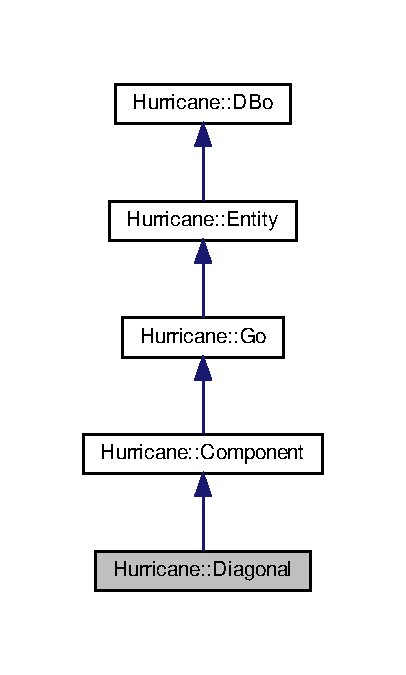
\includegraphics[width=195pt]{classHurricane_1_1Diagonal__inherit__graph}
\end{center}
\end{figure}
\doxysubsection*{Public Types}
\begin{DoxyCompactItemize}
\item 
typedef \mbox{\hyperlink{classHurricane_1_1Component}{Component}} \mbox{\hyperlink{classHurricane_1_1Diagonal_aef5120a04b3b4db78b118e8c5daade90}{Super}}
\end{DoxyCompactItemize}
\doxysubsection*{Static Public Member Functions}
\begin{DoxyCompactItemize}
\item 
static \mbox{\hyperlink{classHurricane_1_1Diagonal}{Diagonal}} $\ast$ \mbox{\hyperlink{classHurricane_1_1Diagonal_a83cd4332e78515e2c3745fd017e7441f}{create}} (\mbox{\hyperlink{classHurricane_1_1Net}{Net}} $\ast$, const \mbox{\hyperlink{classHurricane_1_1Layer}{Layer}} $\ast$, const \mbox{\hyperlink{classHurricane_1_1Point}{Point}} \&source, const \mbox{\hyperlink{classHurricane_1_1Point}{Point}} \&target, \mbox{\hyperlink{classHurricane_1_1DbU_a4fbfa3e8c89347af76c9628ea06c4146}{Db\+U\+::\+Unit}} width)
\end{DoxyCompactItemize}
\doxysubsection*{Additional Inherited Members}


\doxysubsection{Detailed Description}
\mbox{\hyperlink{classHurricane_1_1Diagonal}{Diagonal}} description ({\bfseries{API}}) 

\hypertarget{classHurricane_1_1Diagonal_secDiagonalIntro}{}\doxysubsection{Introduction}\label{classHurricane_1_1Diagonal_secDiagonalIntro}
Create 45° or 135° segments.

The minimal step length for the manhattanisation is set up with Db\+U\+::set\+Diagonal\+Step().

\begin{DoxyWarning}{Warning}
\mbox{\hyperlink{classHurricane_1_1Diagonal}{Diagonal}} objects {\bfseries{cannot}} be exported in symbolic layout. 
\end{DoxyWarning}


\doxysubsection{Member Typedef Documentation}
\mbox{\Hypertarget{classHurricane_1_1Diagonal_aef5120a04b3b4db78b118e8c5daade90}\label{classHurricane_1_1Diagonal_aef5120a04b3b4db78b118e8c5daade90}} 
\index{Hurricane::Diagonal@{Hurricane::Diagonal}!Super@{Super}}
\index{Super@{Super}!Hurricane::Diagonal@{Hurricane::Diagonal}}
\doxysubsubsection{\texorpdfstring{Super}{Super}}
{\footnotesize\ttfamily \mbox{\hyperlink{classHurricane_1_1Diagonal_aef5120a04b3b4db78b118e8c5daade90}{Hurricane\+::\+Diagonal\+::\+Super}}}

Useful for calling upon methods of the base class without knowing it. 

\doxysubsection{Member Function Documentation}
\mbox{\Hypertarget{classHurricane_1_1Diagonal_a83cd4332e78515e2c3745fd017e7441f}\label{classHurricane_1_1Diagonal_a83cd4332e78515e2c3745fd017e7441f}} 
\index{Hurricane::Diagonal@{Hurricane::Diagonal}!create@{create}}
\index{create@{create}!Hurricane::Diagonal@{Hurricane::Diagonal}}
\doxysubsubsection{\texorpdfstring{create()}{create()}}
{\footnotesize\ttfamily \mbox{\hyperlink{classHurricane_1_1Diagonal}{Diagonal}} $\ast$ Hurricane\+::\+Diagonal\+::create (\begin{DoxyParamCaption}\item[{\mbox{\hyperlink{classHurricane_1_1Net}{Net}} $\ast$}]{net,  }\item[{const \mbox{\hyperlink{classHurricane_1_1Layer}{Layer}} $\ast$}]{layer,  }\item[{const \mbox{\hyperlink{classHurricane_1_1Point}{Point}} \&}]{source,  }\item[{const \mbox{\hyperlink{classHurricane_1_1Point}{Point}} \&}]{target,  }\item[{\mbox{\hyperlink{classHurricane_1_1DbU_a4fbfa3e8c89347af76c9628ea06c4146}{Db\+U\+::\+Unit}}}]{width }\end{DoxyParamCaption})\hspace{0.3cm}{\ttfamily [static]}}

Create a diagonal segment of {\ttfamily layer} in {\ttfamily net}. 

The documentation for this class was generated from the following files\+:\begin{DoxyCompactItemize}
\item 
Diagonal.\+h\item 
Diagonal.\+dox\end{DoxyCompactItemize}

\hypertarget{classHurricane_1_1DiffusionLayer}{}\doxysection{Hurricane\+::Diffusion\+Layer Class Reference}
\label{classHurricane_1_1DiffusionLayer}\index{Hurricane::DiffusionLayer@{Hurricane::DiffusionLayer}}


\mbox{\hyperlink{classHurricane_1_1DiffusionLayer}{Diffusion\+Layer}} description ({\bfseries{API}})  




Inheritance diagram for Hurricane\+::Diffusion\+Layer\+:\nopagebreak
\begin{figure}[H]
\begin{center}
\leavevmode
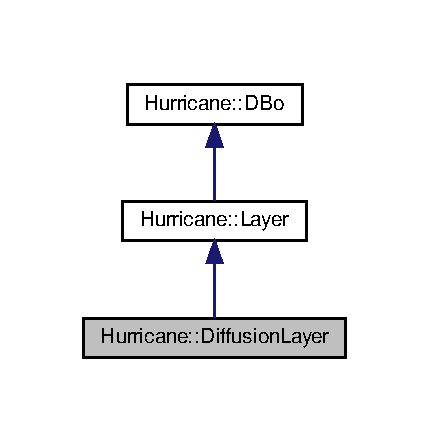
\includegraphics[width=206pt]{classHurricane_1_1DiffusionLayer__inherit__graph}
\end{center}
\end{figure}
\doxysubsection*{Static Public Member Functions}
\begin{DoxyCompactItemize}
\item 
static \mbox{\hyperlink{classHurricane_1_1DiffusionLayer}{Diffusion\+Layer}} $\ast$ \mbox{\hyperlink{classHurricane_1_1DiffusionLayer_a91b5f8a20b005c20b4b9b9080250939e}{create}} (\mbox{\hyperlink{classHurricane_1_1Technology}{Technology}} $\ast$technology, const \mbox{\hyperlink{classHurricane_1_1Name}{Name}} \&name, \mbox{\hyperlink{classHurricane_1_1BasicLayer}{Basic\+Layer}} $\ast$active\+Layer, \mbox{\hyperlink{classHurricane_1_1BasicLayer}{Basic\+Layer}} $\ast$diffusion\+Layer, \mbox{\hyperlink{classHurricane_1_1BasicLayer}{Basic\+Layer}} $\ast$well\+Layer)
\end{DoxyCompactItemize}
\doxysubsection*{Additional Inherited Members}


\doxysubsection{Detailed Description}
\mbox{\hyperlink{classHurricane_1_1DiffusionLayer}{Diffusion\+Layer}} description ({\bfseries{API}}) 

For a more complete description of the Layers objects, please refer to \mbox{\hyperlink{classHurricane_1_1Layer_secLayerIntro}{Layer Introduction}}.

\mbox{\hyperlink{classHurricane_1_1DiffusionLayer}{Diffusion\+Layer}} is a symbolic layer that contains two or three layers, an active layer, a diffusion layer and an optional WELL layer.

The accessors functions\+: 
\begin{DoxyItemize}
\item \mbox{\hyperlink{classHurricane_1_1Layer_a5f7c43a29f3dd02a9ebccbcbf91d6727}{Diffusion\+Layer\+::get\+Top()}} 
\item \mbox{\hyperlink{classHurricane_1_1Layer_a4dab4552a219d2d900ed0b1245dc6580}{Diffusion\+Layer\+::get\+Bottom()}} 
\item \mbox{\hyperlink{classHurricane_1_1Layer_a69e76c09a56260169c4f5c145a35a47f}{Diffusion\+Layer\+::get\+Opposite()}} 
\end{DoxyItemize}Have no meaning here.

Only extention cap \& extention width are used here. Enclosure is not used. 

\doxysubsection{Member Function Documentation}
\mbox{\Hypertarget{classHurricane_1_1DiffusionLayer_a91b5f8a20b005c20b4b9b9080250939e}\label{classHurricane_1_1DiffusionLayer_a91b5f8a20b005c20b4b9b9080250939e}} 
\index{Hurricane::DiffusionLayer@{Hurricane::DiffusionLayer}!create@{create}}
\index{create@{create}!Hurricane::DiffusionLayer@{Hurricane::DiffusionLayer}}
\doxysubsubsection{\texorpdfstring{create()}{create()}}
{\footnotesize\ttfamily \mbox{\hyperlink{classHurricane_1_1DiffusionLayer}{Diffusion\+Layer}} $\ast$ Hurricane\+::\+Diffusion\+Layer\+::create (\begin{DoxyParamCaption}\item[{\mbox{\hyperlink{classHurricane_1_1Technology}{Technology}} $\ast$}]{technology,  }\item[{const \mbox{\hyperlink{classHurricane_1_1Name}{Name}} \&}]{name,  }\item[{\mbox{\hyperlink{classHurricane_1_1BasicLayer}{Basic\+Layer}} $\ast$}]{active\+Layer,  }\item[{\mbox{\hyperlink{classHurricane_1_1BasicLayer}{Basic\+Layer}} $\ast$}]{diffusion\+Layer,  }\item[{\mbox{\hyperlink{classHurricane_1_1BasicLayer}{Basic\+Layer}} $\ast$}]{well\+Layer }\end{DoxyParamCaption})\hspace{0.3cm}{\ttfamily [static]}}

creates and returns a new diffusion layer named {\ttfamily $<$name$>$}, composed of active \& diffusion \mbox{\hyperlink{classHurricane_1_1BasicLayer}{Basic\+Layer}} and an optional WELL \mbox{\hyperlink{classHurricane_1_1BasicLayer}{Basic\+Layer}}. A NULL value indicates that no NWELL is used.

\begin{DoxyParagraph}{Caution\+: Throws an exception if the technology is null, if the name is }
empty, if a layer of same name already exists or if we overflow the capacity of the bit field associated to the layer mask. 
\end{DoxyParagraph}


The documentation for this class was generated from the following files\+:\begin{DoxyCompactItemize}
\item 
Diffusion\+Layer.\+h\item 
Diffusion\+Layer.\+dox\end{DoxyCompactItemize}

\hypertarget{classHurricane_1_1Net_1_1Direction}{}\doxysection{Hurricane\+::Net\+::Direction Class Reference}
\label{classHurricane_1_1Net_1_1Direction}\index{Hurricane::Net::Direction@{Hurricane::Net::Direction}}
\doxysubsection*{Public Types}
\begin{DoxyCompactItemize}
\item 
enum \mbox{\hyperlink{classHurricane_1_1Net_1_1Direction_a5b34d7c3ac52628861af3a46f781fae4}{Code}} \{ \newline
\mbox{\hyperlink{classHurricane_1_1Net_1_1Direction_a5b34d7c3ac52628861af3a46f781fae4a36971421023586a2b5b019f468d699ba}{Dir\+In}} = 0x0001
, \newline
\mbox{\hyperlink{classHurricane_1_1Net_1_1Direction_a5b34d7c3ac52628861af3a46f781fae4a1135f8c6a05d3801c43684bc195f66f0}{Dir\+Out}} = 0x0002
, \newline
\mbox{\hyperlink{classHurricane_1_1Net_1_1Direction_a5b34d7c3ac52628861af3a46f781fae4a368b35a5f289879ad5c6862dfebc1b96}{Dir\+Undefined}} = 0x0000
, \newline
\mbox{\hyperlink{classHurricane_1_1Net_1_1Direction_a5b34d7c3ac52628861af3a46f781fae4afa0b4523129378e11f6e9bdc72fba627}{Conn\+Tristate}} = 0x0100
, \newline
\mbox{\hyperlink{classHurricane_1_1Net_1_1Direction_a5b34d7c3ac52628861af3a46f781fae4a03861307a54d5204f34c74365aa58f04}{Conn\+Wired\+Or}} = 0x0200
, \newline
\mbox{\hyperlink{classHurricane_1_1Net_1_1Direction_a5b34d7c3ac52628861af3a46f781fae4ad15ab42a0127de740e1c2c05841c153a}{UNDEFINED}} = Dir\+Undefined
, \newline
\mbox{\hyperlink{classHurricane_1_1Net_1_1Direction_a5b34d7c3ac52628861af3a46f781fae4aae6e926e7787f90824a4ee961e6ddac1}{IN}} = Dir\+In
, \newline
\mbox{\hyperlink{classHurricane_1_1Net_1_1Direction_a5b34d7c3ac52628861af3a46f781fae4a2dac58452d767718df817bcf65906969}{OUT}} = Dir\+Out
, \newline
\mbox{\hyperlink{classHurricane_1_1Net_1_1Direction_a5b34d7c3ac52628861af3a46f781fae4aa88aea57d992b95a08c24716b5265afd}{INOUT}} = Dir\+In $\vert$ Dir\+Out
, \newline
\mbox{\hyperlink{classHurricane_1_1Net_1_1Direction_a5b34d7c3ac52628861af3a46f781fae4a71a487a8129c354630d5e989d3994c98}{TRISTATE}} = Dir\+Out $\vert$ Conn\+Tristate
, \newline
\mbox{\hyperlink{classHurricane_1_1Net_1_1Direction_a5b34d7c3ac52628861af3a46f781fae4ab8965ba57b68fc4b58c428fc4c8da397}{TRANSCV}} = Dir\+In $\vert$ Dir\+Out $\vert$ Conn\+Tristate
, \newline
\mbox{\hyperlink{classHurricane_1_1Net_1_1Direction_a5b34d7c3ac52628861af3a46f781fae4a1cc48f96bc28740eb7f0d7ba7e2b237c}{WOR\+\_\+\+OUT}} = Dir\+Out $\vert$ Conn\+Wired\+Or
, \newline
\mbox{\hyperlink{classHurricane_1_1Net_1_1Direction_a5b34d7c3ac52628861af3a46f781fae4a2fbc95d7882aab3453d5549493763c3c}{WOR\+\_\+\+INOUT}} = Dir\+In $\vert$ Dir\+Out $\vert$ Conn\+Wired\+Or
, \newline
{\bfseries Dir\+Mask} = Dir\+In $\vert$ Dir\+Out $\vert$ Dir\+Undefined
 \}
\end{DoxyCompactItemize}


\doxysubsection{Detailed Description}
Encapsulate the \mbox{\hyperlink{classHurricane_1_1Net_1_1Direction_a5b34d7c3ac52628861af3a46f781fae4}{Net\+::\+Direction\+::\+Code}} enumeration that defines the signal direction. This direction is meaningful for external nets only. 

\doxysubsection{Member Enumeration Documentation}
\mbox{\Hypertarget{classHurricane_1_1Net_1_1Direction_a5b34d7c3ac52628861af3a46f781fae4}\label{classHurricane_1_1Net_1_1Direction_a5b34d7c3ac52628861af3a46f781fae4}} 
\index{Hurricane::Net::Direction@{Hurricane::Net::Direction}!Code@{Code}}
\index{Code@{Code}!Hurricane::Net::Direction@{Hurricane::Net::Direction}}
\doxysubsubsection{\texorpdfstring{Code}{Code}}
{\footnotesize\ttfamily enum \mbox{\hyperlink{classHurricane_1_1Net_1_1Direction_a5b34d7c3ac52628861af3a46f781fae4}{Hurricane\+::\+Net\+::\+Direction\+::\+Code}}}

This enumeration defines the signal direction inside the \mbox{\hyperlink{classHurricane_1_1Net_1_1Direction}{Net\+::\+Direction}}. It is build upon two kind of atomic flags, one telling were the sources and sinks are located regarding the \mbox{\hyperlink{classHurricane_1_1Cell}{Cell}} and the other indicating the nature of the driver (normal, tristate, wired-\/or). \begin{DoxyEnumFields}{Enumerator}
\raisebox{\heightof{T}}[0pt][0pt]{\index{DirIn@{DirIn}!Hurricane::Net::Direction@{Hurricane::Net::Direction}}\index{Hurricane::Net::Direction@{Hurricane::Net::Direction}!DirIn@{DirIn}}}\mbox{\Hypertarget{classHurricane_1_1Net_1_1Direction_a5b34d7c3ac52628861af3a46f781fae4a36971421023586a2b5b019f468d699ba}\label{classHurricane_1_1Net_1_1Direction_a5b34d7c3ac52628861af3a46f781fae4a36971421023586a2b5b019f468d699ba}} 
Dir\+In&There is at least one sink on this net ({\itshape atomic}). \\
\hline

\raisebox{\heightof{T}}[0pt][0pt]{\index{DirOut@{DirOut}!Hurricane::Net::Direction@{Hurricane::Net::Direction}}\index{Hurricane::Net::Direction@{Hurricane::Net::Direction}!DirOut@{DirOut}}}\mbox{\Hypertarget{classHurricane_1_1Net_1_1Direction_a5b34d7c3ac52628861af3a46f781fae4a1135f8c6a05d3801c43684bc195f66f0}\label{classHurricane_1_1Net_1_1Direction_a5b34d7c3ac52628861af3a46f781fae4a1135f8c6a05d3801c43684bc195f66f0}} 
Dir\+Out&There is at least one source on this net ({\itshape atomic}). \\
\hline

\raisebox{\heightof{T}}[0pt][0pt]{\index{DirUndefined@{DirUndefined}!Hurricane::Net::Direction@{Hurricane::Net::Direction}}\index{Hurricane::Net::Direction@{Hurricane::Net::Direction}!DirUndefined@{DirUndefined}}}\mbox{\Hypertarget{classHurricane_1_1Net_1_1Direction_a5b34d7c3ac52628861af3a46f781fae4a368b35a5f289879ad5c6862dfebc1b96}\label{classHurricane_1_1Net_1_1Direction_a5b34d7c3ac52628861af3a46f781fae4a368b35a5f289879ad5c6862dfebc1b96}} 
Dir\+Undefined&Undefined direction ({\itshape atomic}). \\
\hline

\raisebox{\heightof{T}}[0pt][0pt]{\index{ConnTristate@{ConnTristate}!Hurricane::Net::Direction@{Hurricane::Net::Direction}}\index{Hurricane::Net::Direction@{Hurricane::Net::Direction}!ConnTristate@{ConnTristate}}}\mbox{\Hypertarget{classHurricane_1_1Net_1_1Direction_a5b34d7c3ac52628861af3a46f781fae4afa0b4523129378e11f6e9bdc72fba627}\label{classHurricane_1_1Net_1_1Direction_a5b34d7c3ac52628861af3a46f781fae4afa0b4523129378e11f6e9bdc72fba627}} 
Conn\+Tristate&The sources are {\bfseries{tristates}}, this a bus ({\itshape atomic}). \\
\hline

\raisebox{\heightof{T}}[0pt][0pt]{\index{ConnWiredOr@{ConnWiredOr}!Hurricane::Net::Direction@{Hurricane::Net::Direction}}\index{Hurricane::Net::Direction@{Hurricane::Net::Direction}!ConnWiredOr@{ConnWiredOr}}}\mbox{\Hypertarget{classHurricane_1_1Net_1_1Direction_a5b34d7c3ac52628861af3a46f781fae4a03861307a54d5204f34c74365aa58f04}\label{classHurricane_1_1Net_1_1Direction_a5b34d7c3ac52628861af3a46f781fae4a03861307a54d5204f34c74365aa58f04}} 
Conn\+Wired\+Or&The sources are {\bfseries{wired or}}, this a bus ({\itshape atomic}). \\
\hline

\raisebox{\heightof{T}}[0pt][0pt]{\index{UNDEFINED@{UNDEFINED}!Hurricane::Net::Direction@{Hurricane::Net::Direction}}\index{Hurricane::Net::Direction@{Hurricane::Net::Direction}!UNDEFINED@{UNDEFINED}}}\mbox{\Hypertarget{classHurricane_1_1Net_1_1Direction_a5b34d7c3ac52628861af3a46f781fae4ad15ab42a0127de740e1c2c05841c153a}\label{classHurricane_1_1Net_1_1Direction_a5b34d7c3ac52628861af3a46f781fae4ad15ab42a0127de740e1c2c05841c153a}} 
UNDEFINED&Undefined direction. \\
\hline

\raisebox{\heightof{T}}[0pt][0pt]{\index{IN@{IN}!Hurricane::Net::Direction@{Hurricane::Net::Direction}}\index{Hurricane::Net::Direction@{Hurricane::Net::Direction}!IN@{IN}}}\mbox{\Hypertarget{classHurricane_1_1Net_1_1Direction_a5b34d7c3ac52628861af3a46f781fae4aae6e926e7787f90824a4ee961e6ddac1}\label{classHurricane_1_1Net_1_1Direction_a5b34d7c3ac52628861af3a46f781fae4aae6e926e7787f90824a4ee961e6ddac1}} 
IN&There must be only sinks inside and a single permanent driver outside. \\
\hline

\raisebox{\heightof{T}}[0pt][0pt]{\index{OUT@{OUT}!Hurricane::Net::Direction@{Hurricane::Net::Direction}}\index{Hurricane::Net::Direction@{Hurricane::Net::Direction}!OUT@{OUT}}}\mbox{\Hypertarget{classHurricane_1_1Net_1_1Direction_a5b34d7c3ac52628861af3a46f781fae4a2dac58452d767718df817bcf65906969}\label{classHurricane_1_1Net_1_1Direction_a5b34d7c3ac52628861af3a46f781fae4a2dac58452d767718df817bcf65906969}} 
OUT&There must be no driver outside and a single permanent driver inside (and no sinks inside). \\
\hline

\raisebox{\heightof{T}}[0pt][0pt]{\index{INOUT@{INOUT}!Hurricane::Net::Direction@{Hurricane::Net::Direction}}\index{Hurricane::Net::Direction@{Hurricane::Net::Direction}!INOUT@{INOUT}}}\mbox{\Hypertarget{classHurricane_1_1Net_1_1Direction_a5b34d7c3ac52628861af3a46f781fae4aa88aea57d992b95a08c24716b5265afd}\label{classHurricane_1_1Net_1_1Direction_a5b34d7c3ac52628861af3a46f781fae4aa88aea57d992b95a08c24716b5265afd}} 
INOUT&There must be one permanent driver inside withs at least one sink inside. \\
\hline

\raisebox{\heightof{T}}[0pt][0pt]{\index{TRISTATE@{TRISTATE}!Hurricane::Net::Direction@{Hurricane::Net::Direction}}\index{Hurricane::Net::Direction@{Hurricane::Net::Direction}!TRISTATE@{TRISTATE}}}\mbox{\Hypertarget{classHurricane_1_1Net_1_1Direction_a5b34d7c3ac52628861af3a46f781fae4a71a487a8129c354630d5e989d3994c98}\label{classHurricane_1_1Net_1_1Direction_a5b34d7c3ac52628861af3a46f781fae4a71a487a8129c354630d5e989d3994c98}} 
TRISTATE&An OUT signal with a tristate driver (bus). \\
\hline

\raisebox{\heightof{T}}[0pt][0pt]{\index{TRANSCV@{TRANSCV}!Hurricane::Net::Direction@{Hurricane::Net::Direction}}\index{Hurricane::Net::Direction@{Hurricane::Net::Direction}!TRANSCV@{TRANSCV}}}\mbox{\Hypertarget{classHurricane_1_1Net_1_1Direction_a5b34d7c3ac52628861af3a46f781fae4ab8965ba57b68fc4b58c428fc4c8da397}\label{classHurricane_1_1Net_1_1Direction_a5b34d7c3ac52628861af3a46f781fae4ab8965ba57b68fc4b58c428fc4c8da397}} 
TRANSCV&An INOUT signal with a tristate driver (bus). \\
\hline

\raisebox{\heightof{T}}[0pt][0pt]{\index{WOR\_OUT@{WOR\_OUT}!Hurricane::Net::Direction@{Hurricane::Net::Direction}}\index{Hurricane::Net::Direction@{Hurricane::Net::Direction}!WOR\_OUT@{WOR\_OUT}}}\mbox{\Hypertarget{classHurricane_1_1Net_1_1Direction_a5b34d7c3ac52628861af3a46f781fae4a1cc48f96bc28740eb7f0d7ba7e2b237c}\label{classHurricane_1_1Net_1_1Direction_a5b34d7c3ac52628861af3a46f781fae4a1cc48f96bc28740eb7f0d7ba7e2b237c}} 
WOR\+\_\+\+OUT&An OUT signal with a wired-\/or driver (bus). \\
\hline

\raisebox{\heightof{T}}[0pt][0pt]{\index{WOR\_INOUT@{WOR\_INOUT}!Hurricane::Net::Direction@{Hurricane::Net::Direction}}\index{Hurricane::Net::Direction@{Hurricane::Net::Direction}!WOR\_INOUT@{WOR\_INOUT}}}\mbox{\Hypertarget{classHurricane_1_1Net_1_1Direction_a5b34d7c3ac52628861af3a46f781fae4a2fbc95d7882aab3453d5549493763c3c}\label{classHurricane_1_1Net_1_1Direction_a5b34d7c3ac52628861af3a46f781fae4a2fbc95d7882aab3453d5549493763c3c}} 
WOR\+\_\+\+INOUT&An INOUT signal with a wired-\/or driver (bus). \\
\hline

\end{DoxyEnumFields}


The documentation for this class was generated from the following files\+:\begin{DoxyCompactItemize}
\item 
Net.\+h\item 
Net.\+dox\end{DoxyCompactItemize}

\hypertarget{classHurricane_1_1Entity}{}\doxysection{Hurricane\+::Entity Class Reference}
\label{classHurricane_1_1Entity}\index{Hurricane::Entity@{Hurricane::Entity}}


Occurrenceable objects root class ({\bfseries{API}}).  




Inheritance diagram for Hurricane\+::Entity\+:\nopagebreak
\begin{figure}[H]
\begin{center}
\leavevmode
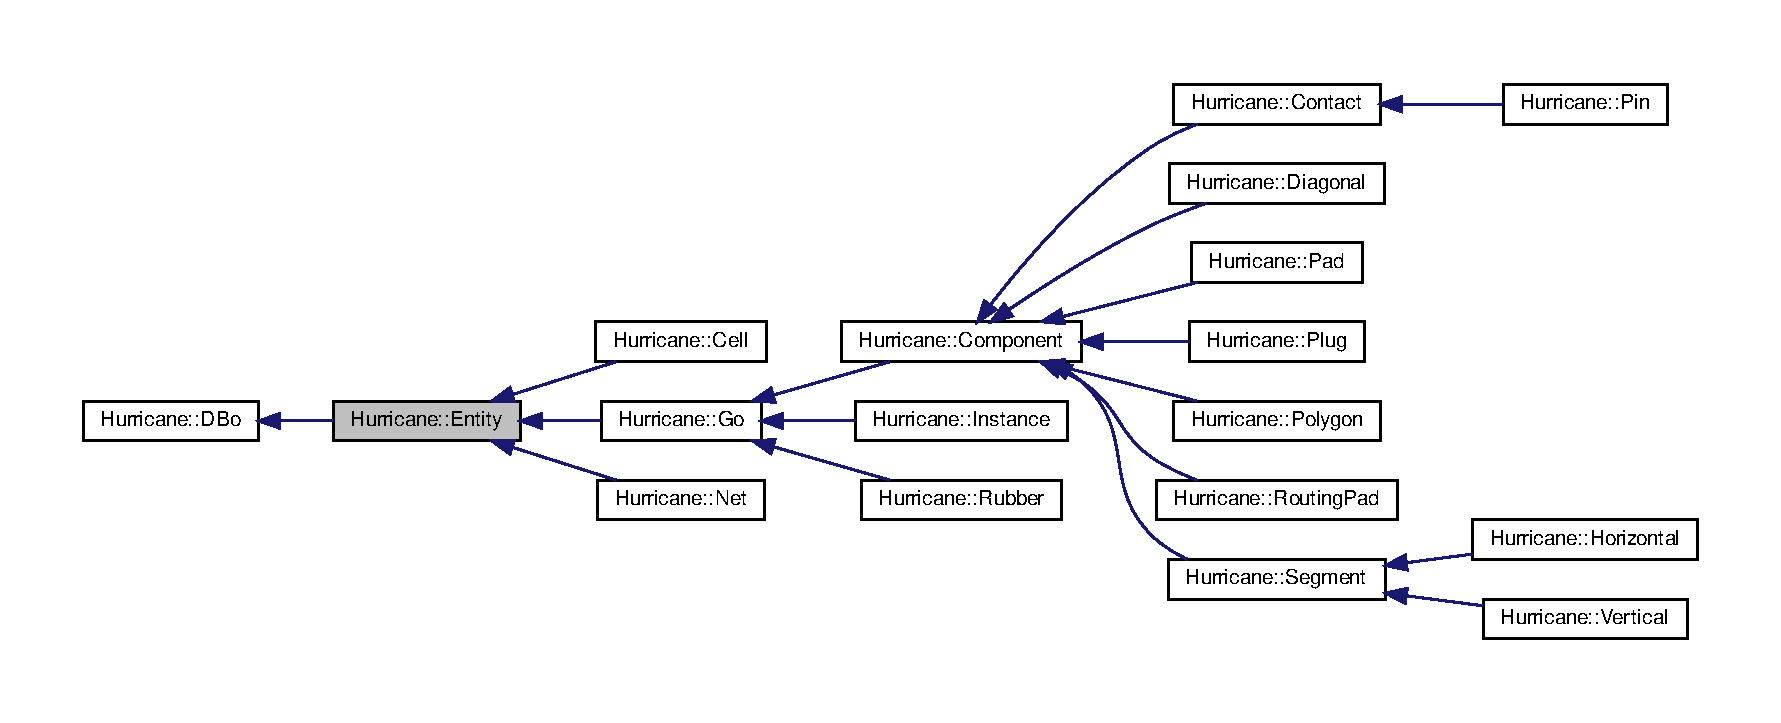
\includegraphics[width=350pt]{classHurricane_1_1Entity__inherit__graph}
\end{center}
\end{figure}
\doxysubsection*{Public Member Functions}
\begin{DoxyCompactItemize}
\item 
virtual \mbox{\hyperlink{classHurricane_1_1Cell}{Cell}} $\ast$ \mbox{\hyperlink{classHurricane_1_1Entity_a42bdf015f583be477cc54b48652b1007}{get\+Cell}} () const =0
\item 
virtual \mbox{\hyperlink{classHurricane_1_1Box}{Box}} \mbox{\hyperlink{classHurricane_1_1Entity_ad834f8ce33a08a13e2a88446696e63e7}{get\+Bounding\+Box}} () const =0
\end{DoxyCompactItemize}


\doxysubsection{Detailed Description}
Occurrenceable objects root class ({\bfseries{API}}). 

\hypertarget{classHurricane_1_1Entity_secEntityIntro}{}\doxysubsection{Introduction}\label{classHurricane_1_1Entity_secEntityIntro}
Entities are abstract objects representing the category of occurrenceable objects.\hypertarget{classHurricane_1_1Entity_secEntityId}{}\doxysubsection{Unique Identifier}\label{classHurricane_1_1Entity_secEntityId}
Each \mbox{\hyperlink{classHurricane_1_1Entity}{Entity}} is associated with a unique identifier (see Entity\+::get\+Id()). This identifier is used as a sorting key in the various Intrusive\+Map throughout \mbox{\hyperlink{namespaceHurricane}{Hurricane}} to ensure determinism. It came as a replacement of the object\textquotesingle{}s own address which is not suitable for this purpose.

For STL container, the \mbox{\hyperlink{classEntity_1_1CompareById}{Entity\+::\+Compare\+By\+Id}} functor is provided.

The identifier is generated from an ever incrementing counter on 32 bits or 64 bits, depending on the target system architecture. If the 32/64 bit capacity is reached an exception is thrown. 

\doxysubsection{Member Function Documentation}
\mbox{\Hypertarget{classHurricane_1_1Entity_a42bdf015f583be477cc54b48652b1007}\label{classHurricane_1_1Entity_a42bdf015f583be477cc54b48652b1007}} 
\index{Hurricane::Entity@{Hurricane::Entity}!getCell@{getCell}}
\index{getCell@{getCell}!Hurricane::Entity@{Hurricane::Entity}}
\doxysubsubsection{\texorpdfstring{getCell()}{getCell()}}
{\footnotesize\ttfamily \mbox{\hyperlink{classHurricane_1_1Cell}{Cell}} $\ast$ Hurricane\+::\+Entity\+::get\+Cell (\begin{DoxyParamCaption}{ }\end{DoxyParamCaption}) const\hspace{0.3cm}{\ttfamily [pure virtual]}}

{\bfseries{Returns\+:}} Returns the cell owning this entity (when the \mbox{\hyperlink{classHurricane_1_1Entity}{Entity}} is a \mbox{\hyperlink{classHurricane_1_1Cell}{Cell}}, the \mbox{\hyperlink{classHurricane_1_1Cell}{Cell}} itself is returned) \mbox{\Hypertarget{classHurricane_1_1Entity_ad834f8ce33a08a13e2a88446696e63e7}\label{classHurricane_1_1Entity_ad834f8ce33a08a13e2a88446696e63e7}} 
\index{Hurricane::Entity@{Hurricane::Entity}!getBoundingBox@{getBoundingBox}}
\index{getBoundingBox@{getBoundingBox}!Hurricane::Entity@{Hurricane::Entity}}
\doxysubsubsection{\texorpdfstring{getBoundingBox()}{getBoundingBox()}}
{\footnotesize\ttfamily \mbox{\hyperlink{classHurricane_1_1Box}{Box}} Hurricane\+::\+Entity\+::get\+Bounding\+Box (\begin{DoxyParamCaption}{ }\end{DoxyParamCaption}) const\hspace{0.3cm}{\ttfamily [pure virtual]}}

\begin{DoxyReturn}{Returns}
Returns the bounding box of the entity. It is defined as the smallest box enclosing the entity or its constituents.
\end{DoxyReturn}
\begin{DoxyRemark}{Remarks}
For the Plugs, which are not objects of the physical layout, the returned envelope is a \mbox{\hyperlink{classHurricane_1_1Box}{Box}} of null dimensions (ponctual) centered on the location of the master \mbox{\hyperlink{classHurricane_1_1Net}{Net}} of the \mbox{\hyperlink{classHurricane_1_1Plug}{Plug}}, to which has been applied the transformation associated to the \mbox{\hyperlink{classHurricane_1_1Instance}{Instance}} of the \mbox{\hyperlink{classHurricane_1_1Plug}{Plug}}. 
\end{DoxyRemark}


Implemented in \mbox{\hyperlink{classHurricane_1_1RoutingPad_a2cc2894b5e1c82b725dedcf1978dc773}{Hurricane\+::\+Routing\+Pad}}.



The documentation for this class was generated from the following files\+:\begin{DoxyCompactItemize}
\item 
Entity.\+h\item 
Entity.\+dox\end{DoxyCompactItemize}

\hypertarget{classHurricane_1_1Error}{}\doxysection{Hurricane\+::Error Class Reference}
\label{classHurricane_1_1Error}\index{Hurricane::Error@{Hurricane::Error}}


\mbox{\hyperlink{classHurricane_1_1Error}{Error}} description ({\bfseries{API}})  




Inheritance diagram for Hurricane\+::Error\+:\nopagebreak
\begin{figure}[H]
\begin{center}
\leavevmode
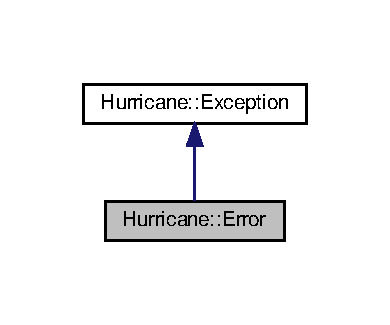
\includegraphics[width=187pt]{classHurricane_1_1Error__inherit__graph}
\end{center}
\end{figure}
\doxysubsection*{Public Member Functions}
\begin{DoxyCompactItemize}
\item 
\mbox{\hyperlink{classHurricane_1_1Error_ab58387c890740ed8082532c5342f2d03}{Error}} (const string \&reason)
\item 
\mbox{\hyperlink{classHurricane_1_1Error_a98f50dcce8258982d450e8f5f79cff38}{Error}} (const char $\ast$format,...)
\item 
\mbox{\hyperlink{classHurricane_1_1Error_a33e4d2a1ea71be6395dc2716b68378c8}{Error}} (int code, const string \&reason)
\item 
\mbox{\hyperlink{classHurricane_1_1Error_a32ccc14fe29d7d2a7b5fe66ee0a3845c}{Error}} (int code, const char $\ast$format,...)
\item 
\mbox{\hyperlink{classHurricane_1_1Error_a7d90d5f5727dab2a9cc0a6427fb2b084}{Error}} (const \mbox{\hyperlink{classHurricane_1_1Error}{Error}} \&error)
\item 
string \mbox{\hyperlink{classHurricane_1_1Error_a1a18927a2d4eb2b0b0acfc2908be7008}{get\+Reason}} () const
\item 
int \mbox{\hyperlink{classHurricane_1_1Error_a1ba11c6ba6eff9fdf2923520fe80a6b2}{get\+Code}} () const
\item 
string \mbox{\hyperlink{classHurricane_1_1Error_ab3b8bb521802f332340eaf0b37eb1dfc}{text\+Where}} () const
\item 
string \mbox{\hyperlink{classHurricane_1_1Error_afafcbeae105f75906c7c45024de41c18}{html\+Where}} () const
\end{DoxyCompactItemize}
\doxysubsection*{Additional Inherited Members}


\doxysubsection{Detailed Description}
\mbox{\hyperlink{classHurricane_1_1Error}{Error}} description ({\bfseries{API}}) 

\hypertarget{classHurricane_1_1Error_secErrorPrintingFormat}{}\doxysubsection{Printing format}\label{classHurricane_1_1Error_secErrorPrintingFormat}
Errors are printed with different formats wether the error code is null or not \+: text\+: So the following code \+: 
\begin{DoxyCode}{0}
\DoxyCodeLine{\textcolor{keywordflow}{try} \{}
\DoxyCodeLine{   \textcolor{keywordflow}{throw} \mbox{\hyperlink{classHurricane_1_1Error_ab58387c890740ed8082532c5342f2d03}{Error}}(\textcolor{stringliteral}{"{}Something strange"{}});}
\DoxyCodeLine{\}}
\DoxyCodeLine{\textcolor{keywordflow}{catch} \{Exception\& exception) \{}
\DoxyCodeLine{   cerr << exception.what() << endl;}
\DoxyCodeLine{\}}

\end{DoxyCode}
 Will produce the message \+: 
\begin{DoxyCode}{0}
\DoxyCodeLine{[ERROR] Something strange}

\end{DoxyCode}
 while the following code \+: 
\begin{DoxyCode}{0}
\DoxyCodeLine{\textcolor{keywordflow}{try} \{}
\DoxyCodeLine{   \textcolor{keywordflow}{throw} \mbox{\hyperlink{classHurricane_1_1Error_ab58387c890740ed8082532c5342f2d03}{Error}}(3, \textcolor{stringliteral}{"{}Can't create Net : null cell"{}});}
\DoxyCodeLine{\}}
\DoxyCodeLine{\textcolor{keywordflow}{catch} \{Exception\& exception) \{}
\DoxyCodeLine{   cerr << exception.what() << endl;}
\DoxyCodeLine{\}}

\end{DoxyCode}
 Will produce the message \+: 
\begin{DoxyCode}{0}
\DoxyCodeLine{[ERROR:3] Can\textcolor{stringliteral}{'t create Net : null cell}}

\end{DoxyCode}
 You can always print something different as shown in the following code \+: 
\begin{DoxyCode}{0}
\DoxyCodeLine{\textcolor{keywordflow}{try} \{}
\DoxyCodeLine{   \textcolor{keywordflow}{throw} \mbox{\hyperlink{classHurricane_1_1Error_ab58387c890740ed8082532c5342f2d03}{Error}}(3, \textcolor{stringliteral}{"{}Can't create Net : null cell"{}});}
\DoxyCodeLine{\}}
\DoxyCodeLine{\textcolor{keywordflow}{catch} \{\mbox{\hyperlink{classHurricane_1_1Error_ab58387c890740ed8082532c5342f2d03}{Error}}\& error) \{}
\DoxyCodeLine{   cerr << error.getReason() << \textcolor{stringliteral}{"{} (code "{}} << error.getCode() << \textcolor{stringliteral}{"{})"{}} << endl;}
\DoxyCodeLine{\}}
\DoxyCodeLine{\textcolor{keywordflow}{catch} \{Exception\& exception) \{}
\DoxyCodeLine{   cerr << exception.what() << endl;}
\DoxyCodeLine{\}}

\end{DoxyCode}
 Which will produce the message \+: 
\begin{DoxyCode}{0}
\DoxyCodeLine{Can\textcolor{stringliteral}{'t create Net : null cell (code 3)}}

\end{DoxyCode}
 

\doxysubsection{Constructor \& Destructor Documentation}
\mbox{\Hypertarget{classHurricane_1_1Error_ab58387c890740ed8082532c5342f2d03}\label{classHurricane_1_1Error_ab58387c890740ed8082532c5342f2d03}} 
\index{Hurricane::Error@{Hurricane::Error}!Error@{Error}}
\index{Error@{Error}!Hurricane::Error@{Hurricane::Error}}
\doxysubsubsection{\texorpdfstring{Error()}{Error()}\hspace{0.1cm}{\footnotesize\ttfamily [1/5]}}
{\footnotesize\ttfamily Hurricane\+::\+Error\+::\+Error (\begin{DoxyParamCaption}\item[{const string \&}]{reason }\end{DoxyParamCaption})}

Builds a error characterized by a reason (code defaults to zero). \mbox{\Hypertarget{classHurricane_1_1Error_a98f50dcce8258982d450e8f5f79cff38}\label{classHurricane_1_1Error_a98f50dcce8258982d450e8f5f79cff38}} 
\index{Hurricane::Error@{Hurricane::Error}!Error@{Error}}
\index{Error@{Error}!Hurricane::Error@{Hurricane::Error}}
\doxysubsubsection{\texorpdfstring{Error()}{Error()}\hspace{0.1cm}{\footnotesize\ttfamily [2/5]}}
{\footnotesize\ttfamily Hurricane\+::\+Error\+::\+Error (\begin{DoxyParamCaption}\item[{const char $\ast$}]{format,  }\item[{}]{... }\end{DoxyParamCaption})}

Builds a error characterized by a reason, using the {\ttfamily vararg} protocol and {\ttfamily printf} format (code defaults to zero). \mbox{\Hypertarget{classHurricane_1_1Error_a33e4d2a1ea71be6395dc2716b68378c8}\label{classHurricane_1_1Error_a33e4d2a1ea71be6395dc2716b68378c8}} 
\index{Hurricane::Error@{Hurricane::Error}!Error@{Error}}
\index{Error@{Error}!Hurricane::Error@{Hurricane::Error}}
\doxysubsubsection{\texorpdfstring{Error()}{Error()}\hspace{0.1cm}{\footnotesize\ttfamily [3/5]}}
{\footnotesize\ttfamily Hurricane\+::\+Error\+::\+Error (\begin{DoxyParamCaption}\item[{int}]{code,  }\item[{const string \&}]{reason }\end{DoxyParamCaption})}

Builds a error characterized by a reason and a code useful within a switch. \mbox{\Hypertarget{classHurricane_1_1Error_a32ccc14fe29d7d2a7b5fe66ee0a3845c}\label{classHurricane_1_1Error_a32ccc14fe29d7d2a7b5fe66ee0a3845c}} 
\index{Hurricane::Error@{Hurricane::Error}!Error@{Error}}
\index{Error@{Error}!Hurricane::Error@{Hurricane::Error}}
\doxysubsubsection{\texorpdfstring{Error()}{Error()}\hspace{0.1cm}{\footnotesize\ttfamily [4/5]}}
{\footnotesize\ttfamily Hurricane\+::\+Error\+::\+Error (\begin{DoxyParamCaption}\item[{int}]{code,  }\item[{const char $\ast$}]{format,  }\item[{}]{... }\end{DoxyParamCaption})}

Builds a error characterized by a reason and a code useful within a switch. The reason is supplied in a {\ttfamily printf} like fashion. \mbox{\Hypertarget{classHurricane_1_1Error_a7d90d5f5727dab2a9cc0a6427fb2b084}\label{classHurricane_1_1Error_a7d90d5f5727dab2a9cc0a6427fb2b084}} 
\index{Hurricane::Error@{Hurricane::Error}!Error@{Error}}
\index{Error@{Error}!Hurricane::Error@{Hurricane::Error}}
\doxysubsubsection{\texorpdfstring{Error()}{Error()}\hspace{0.1cm}{\footnotesize\ttfamily [5/5]}}
{\footnotesize\ttfamily Hurricane\+::\+Error\+::\+Error (\begin{DoxyParamCaption}\item[{const \mbox{\hyperlink{classHurricane_1_1Error}{Error}} \&}]{error }\end{DoxyParamCaption})}

Copy constructor. 

\doxysubsection{Member Function Documentation}
\mbox{\Hypertarget{classHurricane_1_1Error_a1a18927a2d4eb2b0b0acfc2908be7008}\label{classHurricane_1_1Error_a1a18927a2d4eb2b0b0acfc2908be7008}} 
\index{Hurricane::Error@{Hurricane::Error}!getReason@{getReason}}
\index{getReason@{getReason}!Hurricane::Error@{Hurricane::Error}}
\doxysubsubsection{\texorpdfstring{getReason()}{getReason()}}
{\footnotesize\ttfamily string Hurricane\+::\+Error\+::get\+Reason (\begin{DoxyParamCaption}{ }\end{DoxyParamCaption}) const\hspace{0.3cm}{\ttfamily [inline]}}

{\bfseries{Returns\+:}} the reason for which the error was thrown. \mbox{\Hypertarget{classHurricane_1_1Error_a1ba11c6ba6eff9fdf2923520fe80a6b2}\label{classHurricane_1_1Error_a1ba11c6ba6eff9fdf2923520fe80a6b2}} 
\index{Hurricane::Error@{Hurricane::Error}!getCode@{getCode}}
\index{getCode@{getCode}!Hurricane::Error@{Hurricane::Error}}
\doxysubsubsection{\texorpdfstring{getCode()}{getCode()}}
{\footnotesize\ttfamily int Hurricane\+::\+Error\+::get\+Code (\begin{DoxyParamCaption}{ }\end{DoxyParamCaption}) const\hspace{0.3cm}{\ttfamily [inline]}}

{\bfseries{Returns\+:}} the error code number. \mbox{\Hypertarget{classHurricane_1_1Error_ab3b8bb521802f332340eaf0b37eb1dfc}\label{classHurricane_1_1Error_ab3b8bb521802f332340eaf0b37eb1dfc}} 
\index{Hurricane::Error@{Hurricane::Error}!textWhere@{textWhere}}
\index{textWhere@{textWhere}!Hurricane::Error@{Hurricane::Error}}
\doxysubsubsection{\texorpdfstring{textWhere()}{textWhere()}}
{\footnotesize\ttfamily string Hurricane\+::\+Error\+::text\+Where (\begin{DoxyParamCaption}{ }\end{DoxyParamCaption}) const\hspace{0.3cm}{\ttfamily [inline]}}

{\bfseries{Returns\+:}} A stack trace, suitable for tty. \mbox{\Hypertarget{classHurricane_1_1Error_afafcbeae105f75906c7c45024de41c18}\label{classHurricane_1_1Error_afafcbeae105f75906c7c45024de41c18}} 
\index{Hurricane::Error@{Hurricane::Error}!htmlWhere@{htmlWhere}}
\index{htmlWhere@{htmlWhere}!Hurricane::Error@{Hurricane::Error}}
\doxysubsubsection{\texorpdfstring{htmlWhere()}{htmlWhere()}}
{\footnotesize\ttfamily string Hurricane\+::\+Error\+::html\+Where (\begin{DoxyParamCaption}{ }\end{DoxyParamCaption}) const\hspace{0.3cm}{\ttfamily [inline]}}

{\bfseries{Returns\+:}} A stack trace, suitable for HTML. 

The documentation for this class was generated from the following files\+:\begin{DoxyCompactItemize}
\item 
Error.\+h\item 
Error.\+dox\end{DoxyCompactItemize}

\hypertarget{classHurricane_1_1Exception}{}\doxysection{Hurricane\+::Exception Class Reference}
\label{classHurricane_1_1Exception}\index{Hurricane::Exception@{Hurricane::Exception}}


\mbox{\hyperlink{classHurricane_1_1Exception}{Exception}} description ({\bfseries{API}})  




Inheritance diagram for Hurricane\+::Exception\+:\nopagebreak
\begin{figure}[H]
\begin{center}
\leavevmode
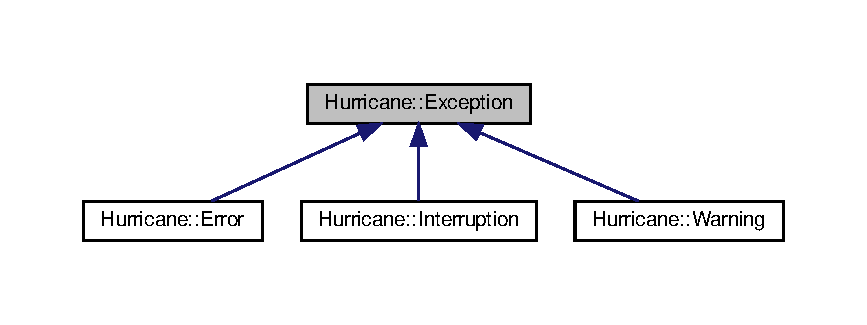
\includegraphics[width=350pt]{classHurricane_1_1Exception__inherit__graph}
\end{center}
\end{figure}
\doxysubsection*{Public Member Functions}
\begin{DoxyCompactItemize}
\item 
string \mbox{\hyperlink{classHurricane_1_1Exception_a6d8036af345628567494eeab9c8e2e3a}{what}} () const
\item 
string \mbox{\hyperlink{classHurricane_1_1Exception_a19b5d24e8f02bb99625a5206638c44e8}{text\+What}} () const
\item 
string \mbox{\hyperlink{classHurricane_1_1Exception_a2582e6c3acb236e24f48cb873f64e3e9}{html\+What}} () const
\end{DoxyCompactItemize}
\doxysubsection*{Static Public Member Functions}
\begin{DoxyCompactItemize}
\item 
static void \mbox{\hyperlink{classHurricane_1_1Exception_a1a57fbbc4b57a014558ba31d18ec9b62}{set\+Text\+Translator}} (const Text\+Translator \&translator)
\item 
static void \mbox{\hyperlink{classHurricane_1_1Exception_a0effe808df00f4efe10925131304b8d0}{set\+Html\+Translator}} (const Text\+Translator \&translator)
\end{DoxyCompactItemize}


\doxysubsection{Detailed Description}
\mbox{\hyperlink{classHurricane_1_1Exception}{Exception}} description ({\bfseries{API}}) 

\hypertarget{classHurricane_1_1Exception_secExceptionIntro}{}\doxysubsection{Introduction}\label{classHurricane_1_1Exception_secExceptionIntro}
The \mbox{\hyperlink{classHurricane_1_1Exception}{Exception}} class groups all exceptions thrown by functions from the API. This virtual class is only useful to catch exceptions originating from one of those functions.

\begin{DoxyRemark}{Remarks}
Copy construction is disabled.
\end{DoxyRemark}
\hypertarget{classHurricane_1_1Exception_secExceptionExample}{}\doxysubsection{Example}\label{classHurricane_1_1Exception_secExceptionExample}

\begin{DoxyCode}{0}
\DoxyCodeLine{\textcolor{keywordflow}{try} \{}
\DoxyCodeLine{   \textcolor{comment}{// do something}}
\DoxyCodeLine{\}}
\DoxyCodeLine{\textcolor{keywordflow}{catch} (Exception\& exception) \{}
\DoxyCodeLine{   \textcolor{comment}{// Go through here if the exception comes from a function of the API}}
\DoxyCodeLine{   cerr << exception.what() << endl;}
\DoxyCodeLine{   exit(1);}
\DoxyCodeLine{\}}
\DoxyCodeLine{\textcolor{keywordflow}{catch} (...) \{}
\DoxyCodeLine{   \textcolor{comment}{// Go through here for all other system exceptions}}
\DoxyCodeLine{   cerr << Error(\textcolor{stringliteral}{"{}abnormal termination"{}}) << endl;}
\DoxyCodeLine{   \textcolor{comment}{// We use the Error() in order to get the same kind of printing}}
\DoxyCodeLine{   exit(2);}
\DoxyCodeLine{\}}

\end{DoxyCode}
 

\doxysubsection{Member Function Documentation}
\mbox{\Hypertarget{classHurricane_1_1Exception_a6d8036af345628567494eeab9c8e2e3a}\label{classHurricane_1_1Exception_a6d8036af345628567494eeab9c8e2e3a}} 
\index{Hurricane::Exception@{Hurricane::Exception}!what@{what}}
\index{what@{what}!Hurricane::Exception@{Hurricane::Exception}}
\doxysubsubsection{\texorpdfstring{what()}{what()}}
{\footnotesize\ttfamily string Hurricane\+::\+Exception\+::what (\begin{DoxyParamCaption}{ }\end{DoxyParamCaption}) const\hspace{0.3cm}{\ttfamily [inline]}}

{\bfseries{Returns\+:}} an alias over the \mbox{\hyperlink{classHurricane_1_1Exception_a19b5d24e8f02bb99625a5206638c44e8}{text\+What()}} method for convenience. 

References text\+What().

\mbox{\Hypertarget{classHurricane_1_1Exception_a19b5d24e8f02bb99625a5206638c44e8}\label{classHurricane_1_1Exception_a19b5d24e8f02bb99625a5206638c44e8}} 
\index{Hurricane::Exception@{Hurricane::Exception}!textWhat@{textWhat}}
\index{textWhat@{textWhat}!Hurricane::Exception@{Hurricane::Exception}}
\doxysubsubsection{\texorpdfstring{textWhat()}{textWhat()}}
{\footnotesize\ttfamily string Hurricane\+::\+Exception\+::text\+What (\begin{DoxyParamCaption}{ }\end{DoxyParamCaption}) const\hspace{0.3cm}{\ttfamily [inline]}}

{\bfseries{Returns\+:}} an informative (hopefully) about what has caused the exception to occurs. Formatted for an output on a tty.

\begin{DoxySeeAlso}{See also}
\mbox{\hyperlink{classHurricane_1_1Exception_a1a57fbbc4b57a014558ba31d18ec9b62}{set\+Text\+Translator}} 
\end{DoxySeeAlso}


Referenced by what().

\mbox{\Hypertarget{classHurricane_1_1Exception_a2582e6c3acb236e24f48cb873f64e3e9}\label{classHurricane_1_1Exception_a2582e6c3acb236e24f48cb873f64e3e9}} 
\index{Hurricane::Exception@{Hurricane::Exception}!htmlWhat@{htmlWhat}}
\index{htmlWhat@{htmlWhat}!Hurricane::Exception@{Hurricane::Exception}}
\doxysubsubsection{\texorpdfstring{htmlWhat()}{htmlWhat()}}
{\footnotesize\ttfamily string Hurricane\+::\+Exception\+::html\+What (\begin{DoxyParamCaption}{ }\end{DoxyParamCaption}) const\hspace{0.3cm}{\ttfamily [inline]}}

{\bfseries{Returns\+:}} an informative (hopefully) about what has caused the exception to occurs. Formatted for an output on a HTML capable device.

\begin{DoxySeeAlso}{See also}
\mbox{\hyperlink{classHurricane_1_1Exception_a0effe808df00f4efe10925131304b8d0}{set\+Html\+Translator}} 
\end{DoxySeeAlso}
\mbox{\Hypertarget{classHurricane_1_1Exception_a1a57fbbc4b57a014558ba31d18ec9b62}\label{classHurricane_1_1Exception_a1a57fbbc4b57a014558ba31d18ec9b62}} 
\index{Hurricane::Exception@{Hurricane::Exception}!setTextTranslator@{setTextTranslator}}
\index{setTextTranslator@{setTextTranslator}!Hurricane::Exception@{Hurricane::Exception}}
\doxysubsubsection{\texorpdfstring{setTextTranslator()}{setTextTranslator()}}
{\footnotesize\ttfamily string Hurricane\+::\+Exception\+::set\+Text\+Translator (\begin{DoxyParamCaption}\item[{const Text\+Translator \&}]{translator }\end{DoxyParamCaption})\hspace{0.3cm}{\ttfamily [inline]}, {\ttfamily [static]}}

Set the translator used for text (tty) output. \mbox{\Hypertarget{classHurricane_1_1Exception_a0effe808df00f4efe10925131304b8d0}\label{classHurricane_1_1Exception_a0effe808df00f4efe10925131304b8d0}} 
\index{Hurricane::Exception@{Hurricane::Exception}!setHtmlTranslator@{setHtmlTranslator}}
\index{setHtmlTranslator@{setHtmlTranslator}!Hurricane::Exception@{Hurricane::Exception}}
\doxysubsubsection{\texorpdfstring{setHtmlTranslator()}{setHtmlTranslator()}}
{\footnotesize\ttfamily string Hurricane\+::\+Exception\+::set\+Html\+Translator (\begin{DoxyParamCaption}\item[{const Text\+Translator \&}]{translator }\end{DoxyParamCaption})\hspace{0.3cm}{\ttfamily [inline]}, {\ttfamily [static]}}

Set the translator used for HTML (hint\+: Qt manage simple HTML in text) output. 

The documentation for this class was generated from the following files\+:\begin{DoxyCompactItemize}
\item 
Exception.\+h\item 
Exception.\+dox\end{DoxyCompactItemize}

\hypertarget{classHurricane_1_1Filter}{}\doxysection{Hurricane\+::Filter$<$ Type $>$ Class Template Reference}
\label{classHurricane_1_1Filter}\index{Hurricane::Filter$<$ Type $>$@{Hurricane::Filter$<$ Type $>$}}


\mbox{\hyperlink{classHurricane_1_1Filter}{Filter}} description ({\bfseries{API}})  




Inheritance diagram for Hurricane\+::Filter$<$ Type $>$\+:\nopagebreak
\begin{figure}[H]
\begin{center}
\leavevmode
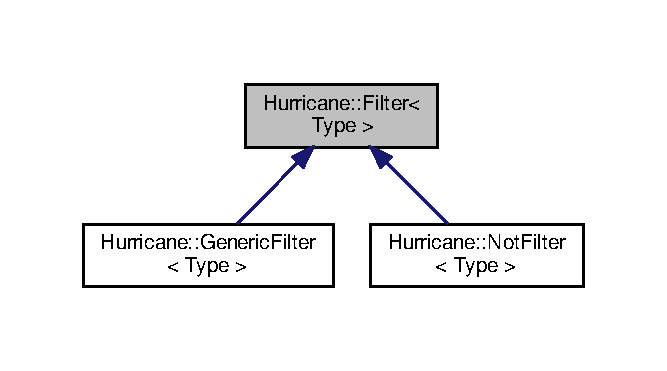
\includegraphics[width=320pt]{classHurricane_1_1Filter__inherit__graph}
\end{center}
\end{figure}
\doxysubsection*{Public Member Functions}
\begin{DoxyCompactItemize}
\item 
\mbox{\hyperlink{classHurricane_1_1GenericFilter}{Generic\+Filter}}$<$ Type $>$ \mbox{\hyperlink{classHurricane_1_1Filter_a90c1a8c4caf6c6018ff50f5b9754e061}{operator!}} () const
\item 
virtual \mbox{\hyperlink{classHurricane_1_1Filter}{Filter}}$<$ Type $>$ $\ast$ \mbox{\hyperlink{classHurricane_1_1Filter_a596cad421801115efbc5c541f8d29e0b}{get\+Clone}} () const =0
\item 
virtual bool \mbox{\hyperlink{classHurricane_1_1Filter_aeaa771f17950fe05273c471ccfffb7f7}{accept}} (Type type) const =0
\end{DoxyCompactItemize}


\doxysubsection{Detailed Description}
\subsubsection*{template$<$class Type$>$\newline
class Hurricane\+::\+Filter$<$ Type $>$}

\mbox{\hyperlink{classHurricane_1_1Filter}{Filter}} description ({\bfseries{API}}) 

\hypertarget{classHurricane_1_1Filter_secFilterIntro}{}\doxysubsection{Introduction}\label{classHurricane_1_1Filter_secFilterIntro}
A filter is a functional object which, used in conjunction with a collection, allows to get only the elements of this collection which meet some criteria.

This class is an abstract class which must be derived in order to get the appropriate behaviour.

You will have also to define the default constructor, the copy constructor, the assignment operator and overload the two following member functions \+:\hypertarget{classHurricane_1_1Filter_secFilterSimpleExample}{}\doxysubsection{Simple Example}\label{classHurricane_1_1Filter_secFilterSimpleExample}
Definition of the filter selecting external nets of a cell \+: 
\begin{DoxyCode}{0}
\DoxyCodeLine{\textcolor{keyword}{class }IsExternal : \textcolor{keyword}{public} Filter<Net*> \{}
\DoxyCodeLine{\textcolor{comment}{// ***********************************}}
\DoxyCodeLine{ }
\DoxyCodeLine{   \textcolor{keyword}{public}:}
\DoxyCodeLine{ }
\DoxyCodeLine{      IsExternal() \{\};}
\DoxyCodeLine{ }
\DoxyCodeLine{      IsExternal(\textcolor{keyword}{const} IsExternal\& isExternal) \{\};}
\DoxyCodeLine{ }
\DoxyCodeLine{      IsExternal\& operator=(\textcolor{keyword}{const} IsExternal\& isExternal) \{\textcolor{keywordflow}{return} *\textcolor{keyword}{this};\};}
\DoxyCodeLine{ }
\DoxyCodeLine{      \textcolor{keyword}{virtual} Filter<Net*>* \mbox{\hyperlink{classHurricane_1_1Filter_a596cad421801115efbc5c541f8d29e0b}{getClone}}()\textcolor{keyword}{ const }\{\textcolor{keywordflow}{return} \textcolor{keyword}{new} IsExternal(*\textcolor{keyword}{this});\};}
\DoxyCodeLine{ }
\DoxyCodeLine{      \textcolor{keyword}{virtual} \textcolor{keywordtype}{bool} \mbox{\hyperlink{classHurricane_1_1Filter_aeaa771f17950fe05273c471ccfffb7f7}{accept}}(Net* net)\textcolor{keyword}{ const }\{\textcolor{keywordflow}{return} net-\/>isExternal();\};}
\DoxyCodeLine{ }
\DoxyCodeLine{\};}

\end{DoxyCode}
 Implementation of the accessor {\bfseries{get\+External\+Nets}} for the cells \+: 
\begin{DoxyCode}{0}
\DoxyCodeLine{\mbox{\hyperlink{namespaceHurricane_a3404a8b17130a1824f4a281704b04df7}{Nets}} Cell::getExternalNet() const}
\DoxyCodeLine{\textcolor{comment}{// ******************************}}
\DoxyCodeLine{\{}
\DoxyCodeLine{   \textcolor{keywordflow}{return} getNets().getSubSet(IsExternal());}
\DoxyCodeLine{\}}

\end{DoxyCode}
 Similarly, the accessor {\bfseries{get\+Internal\+Nets}} can be implemented using the {\bfseries{!}} operator \+: 
\begin{DoxyCode}{0}
\DoxyCodeLine{\mbox{\hyperlink{namespaceHurricane_a3404a8b17130a1824f4a281704b04df7}{Nets}} \mbox{\hyperlink{classHurricane_1_1Cell_a0da980d28ad60334da94a3966338f873}{Cell::getInternalNets}}() const}
\DoxyCodeLine{\textcolor{comment}{// *******************************}}
\DoxyCodeLine{\{}
\DoxyCodeLine{   \textcolor{keywordflow}{return} getNets().\mbox{\hyperlink{classHurricane_1_1Collection_aa32ea7249d57ee05e3c71dcde8106832}{getSubSet}}(!IsExternal());}
\DoxyCodeLine{\}}

\end{DoxyCode}
\hypertarget{classHurricane_1_1Filter_secFilterComplexExample}{}\doxysubsection{Complex Example}\label{classHurricane_1_1Filter_secFilterComplexExample}
In order to implement previous examples we could have used filter with a simpler interface. Now the filters as they are defined open the door to much more complex processing.

As a matter of fact the function {\bfseries{accept}} receives only one argument which represents the element of the collection to be accepted or rejected.

Sometimes the filter must take into account other criteria. For example to print the external nets of a cell whose name start with a given character. Those additional criteria will then become attributes of the filter as shown in the following example \+:

\mbox{\hyperlink{classHurricane_1_1Filter}{Filter}} definition \+: 
\begin{DoxyCode}{0}
\DoxyCodeLine{\textcolor{keyword}{class }MyFilter : \textcolor{keyword}{public} Filter<Net*> \{}
\DoxyCodeLine{\textcolor{comment}{// *********************************}}
\DoxyCodeLine{ }
\DoxyCodeLine{   \textcolor{keyword}{public}:}
\DoxyCodeLine{ }
\DoxyCodeLine{      \textcolor{keywordtype}{char} \_c;}
\DoxyCodeLine{ }
\DoxyCodeLine{      MyFilter(\textcolor{keywordtype}{char} c) : \_c(c) \{\};}
\DoxyCodeLine{ }
\DoxyCodeLine{      MyFilter(\textcolor{keyword}{const} MyFilter\& myFilter) : \_c(myFilter.\_c) \{\};}
\DoxyCodeLine{ }
\DoxyCodeLine{      MyFilter\& operator=(\textcolor{keyword}{const} MyFilter\& myFilter)}
\DoxyCodeLine{      \{}
\DoxyCodeLine{         \_c = myFilter.\_c;}
\DoxyCodeLine{         \textcolor{keywordflow}{return} *\textcolor{keyword}{this};}
\DoxyCodeLine{      \};}
\DoxyCodeLine{ }
\DoxyCodeLine{      \textcolor{keyword}{virtual} Filter<Net*>* \mbox{\hyperlink{classHurricane_1_1Filter_a596cad421801115efbc5c541f8d29e0b}{getClone}}()\textcolor{keyword}{ const }\{\textcolor{keywordflow}{return} \textcolor{keyword}{new} MyFilter(*\textcolor{keyword}{this});\};}
\DoxyCodeLine{ }
\DoxyCodeLine{      \textcolor{keyword}{virtual} \textcolor{keywordtype}{bool} \mbox{\hyperlink{classHurricane_1_1Filter_aeaa771f17950fe05273c471ccfffb7f7}{accept}}(Net* net)\textcolor{keyword}{ const}}
\DoxyCodeLine{\textcolor{keyword}{      }\{}
\DoxyCodeLine{         \textcolor{keywordflow}{return} net-\/>isExternal() \&\& (net-\/>getName()[0] == \_c);}
\DoxyCodeLine{      \};}
\DoxyCodeLine{ }
\DoxyCodeLine{\};}

\end{DoxyCode}
 Afterwards do 
\begin{DoxyCode}{0}
\DoxyCodeLine{forEach(Net*, inet, cell-\/>getNets().getSubSet(MyFilter(\textcolor{charliteral}{'k'}))) \{}
\DoxyCodeLine{   assert(inet-\/>isExternal());}
\DoxyCodeLine{   assert(inet-\/>getName()[0] == \textcolor{charliteral}{'k'});}
\DoxyCodeLine{   cerr << \textcolor{stringliteral}{"{}net: "{}} << (*inet) << endl;}
\DoxyCodeLine{\}}

\end{DoxyCode}
 Although this example is not of great interest, it illustrates the way to proceed to create a complex filter. 

\doxysubsection{Member Function Documentation}
\mbox{\Hypertarget{classHurricane_1_1Filter_a90c1a8c4caf6c6018ff50f5b9754e061}\label{classHurricane_1_1Filter_a90c1a8c4caf6c6018ff50f5b9754e061}} 
\index{Hurricane::Filter$<$ Type $>$@{Hurricane::Filter$<$ Type $>$}!operator"!@{operator"!}}
\index{operator"!@{operator"!}!Hurricane::Filter$<$ Type $>$@{Hurricane::Filter$<$ Type $>$}}
\doxysubsubsection{\texorpdfstring{operator"!()}{operator!()}}
{\footnotesize\ttfamily template$<$class Type $>$ \\
\mbox{\hyperlink{classHurricane_1_1GenericFilter}{Generic\+Filter}}$<$ Type $>$ \mbox{\hyperlink{classHurricane_1_1Filter}{Hurricane\+::\+Filter}}$<$ Type $>$\+::operator! (\begin{DoxyParamCaption}{ }\end{DoxyParamCaption}) const\hspace{0.3cm}{\ttfamily [inline]}}

{\bfseries{Returns\+:}} the inverse filter of the filter {\ttfamily $<$this$>$} (accepted elements are those rejected and conversely). \mbox{\Hypertarget{classHurricane_1_1Filter_a596cad421801115efbc5c541f8d29e0b}\label{classHurricane_1_1Filter_a596cad421801115efbc5c541f8d29e0b}} 
\index{Hurricane::Filter$<$ Type $>$@{Hurricane::Filter$<$ Type $>$}!getClone@{getClone}}
\index{getClone@{getClone}!Hurricane::Filter$<$ Type $>$@{Hurricane::Filter$<$ Type $>$}}
\doxysubsubsection{\texorpdfstring{getClone()}{getClone()}}
{\footnotesize\ttfamily template$<$class Type $>$ \\
\mbox{\hyperlink{classHurricane_1_1Filter}{Filter}}$<$ Type $>$ $\ast$ \mbox{\hyperlink{classHurricane_1_1Filter}{Hurricane\+::\+Filter}}$<$ Type $>$\+::get\+Clone (\begin{DoxyParamCaption}{ }\end{DoxyParamCaption}) const\hspace{0.3cm}{\ttfamily [pure virtual]}}

\hypertarget{classHurricane_1_1Filter_secFilterRemarks}{}\doxysubsection{Remarks}\label{classHurricane_1_1Filter_secFilterRemarks}
It is wise to use filters only when it is trully necessary, that is to produce useful collections to be used extensively.

Indeed, for the previous example, preferably write it like this \+: 
\begin{DoxyCode}{0}
\DoxyCodeLine{forEach(Net*, inet, cell-\/>getNets()) \{}
\DoxyCodeLine{   \textcolor{keywordflow}{if} (inet-\/>isExternal() \&\& (inet-\/>getName()[0] == \textcolor{charliteral}{'k'}))}
\DoxyCodeLine{      cerr << \textcolor{stringliteral}{"{}net: "{}} << *net << endl;}
\DoxyCodeLine{\}}

\end{DoxyCode}
 or more simply \+: 
\begin{DoxyCode}{0}
\DoxyCodeLine{forEach(Net*, net, cell-\/>getExternalNets()) \{}
\DoxyCodeLine{   \textcolor{keywordflow}{if} (inet-\/>getName()[0] == \textcolor{charliteral}{'k'})}
\DoxyCodeLine{      cerr << \textcolor{stringliteral}{"{}net: "{}} << *inet << endl;}
\DoxyCodeLine{\}}

\end{DoxyCode}
 Filters are objects like any other \+: they can be passed as function arguments as shown below \+: 
\begin{DoxyCode}{0}
\DoxyCodeLine{\mbox{\hyperlink{namespaceHurricane_a3404a8b17130a1824f4a281704b04df7}{Nets}} \mbox{\hyperlink{classHurricane_1_1Cell_a8b4728abe83e9ec21d7bee1154218279}{Cell::getNets}}(\textcolor{keyword}{const} GenericFilter<Net*>\& filter) \textcolor{keyword}{const}}
\DoxyCodeLine{\textcolor{comment}{// ********************************************************}}
\DoxyCodeLine{\{}
\DoxyCodeLine{   \textcolor{keywordflow}{return} getNets().\mbox{\hyperlink{classHurricane_1_1Collection_aa32ea7249d57ee05e3c71dcde8106832}{getSubSet}}(filter);}
\DoxyCodeLine{\}}

\end{DoxyCode}
 As far as the type {\bfseries{Net\+Filter}} is defined as being a {\bfseries{\mbox{\hyperlink{classHurricane_1_1GenericFilter}{Generic\+Filter}}$<$Net$\ast$$>$}} the previous function can be written like this \+: 
\begin{DoxyCode}{0}
\DoxyCodeLine{\mbox{\hyperlink{namespaceHurricane_a3404a8b17130a1824f4a281704b04df7}{Nets}} \mbox{\hyperlink{classHurricane_1_1Cell_a8b4728abe83e9ec21d7bee1154218279}{Cell::getNets}}(\textcolor{keyword}{const} \mbox{\hyperlink{namespaceHurricane_a0dfd2c5b40325a919d139091312732e9}{NetFilter}}\& filter) \textcolor{keyword}{const}}
\DoxyCodeLine{\textcolor{comment}{// **********************************************}}
\DoxyCodeLine{\{}
\DoxyCodeLine{   \textcolor{keywordflow}{return} getNets().\mbox{\hyperlink{classHurricane_1_1Collection_aa32ea7249d57ee05e3c71dcde8106832}{getSubSet}}(filter);}
\DoxyCodeLine{\}}

\end{DoxyCode}


{\bfseries{Returns\+:}} a filter copy. \mbox{\Hypertarget{classHurricane_1_1Filter_aeaa771f17950fe05273c471ccfffb7f7}\label{classHurricane_1_1Filter_aeaa771f17950fe05273c471ccfffb7f7}} 
\index{Hurricane::Filter$<$ Type $>$@{Hurricane::Filter$<$ Type $>$}!accept@{accept}}
\index{accept@{accept}!Hurricane::Filter$<$ Type $>$@{Hurricane::Filter$<$ Type $>$}}
\doxysubsubsection{\texorpdfstring{accept()}{accept()}}
{\footnotesize\ttfamily template$<$class Type $>$ \\
bool \mbox{\hyperlink{classHurricane_1_1Filter}{Hurricane\+::\+Filter}}$<$ Type $>$\+::accept (\begin{DoxyParamCaption}\item[{Type}]{element }\end{DoxyParamCaption}) const\hspace{0.3cm}{\ttfamily [pure virtual]}}

This member function returns {\bfseries{true}} if the filter accepts the element else {\bfseries{false}}. 

The documentation for this class was generated from the following files\+:\begin{DoxyCompactItemize}
\item 
Filter.\+h\item 
Filter.\+dox\end{DoxyCompactItemize}

\hypertarget{classHurricane_1_1GenericCollection}{}\doxysection{Hurricane\+::Generic\+Collection$<$ Type $>$ Class Template Reference}
\label{classHurricane_1_1GenericCollection}\index{Hurricane::GenericCollection$<$ Type $>$@{Hurricane::GenericCollection$<$ Type $>$}}


Generic \mbox{\hyperlink{classHurricane_1_1Collection}{Collection}} auto-\/pointer.  




Inheritance diagram for Hurricane\+::Generic\+Collection$<$ Type $>$\+:\nopagebreak
\begin{figure}[H]
\begin{center}
\leavevmode
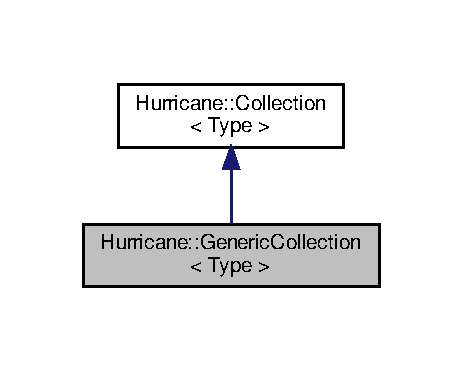
\includegraphics[width=222pt]{classHurricane_1_1GenericCollection__inherit__graph}
\end{center}
\end{figure}
\doxysubsection*{Public Member Functions}
\begin{Indent}\textbf{ Collection Collection}\par
{\em \hypertarget{Collection_8h_secCollectionUtilitarians}{}\doxysubsection{Utilitarians}\label{Collection_8h_secCollectionUtilitarians}
{\bfseries{Collection\+::\+Fill}} {\bfseries{Collection\+::\+Fill}} {\bfseries{Collection\+::\+Fill}} \begin{DoxyRemark}{Remarks}
The elements are added to the container in the order with which the collection is visited. So the same order will appear in a list or a vector, but for a set they will be inserted according to the set ordering method. 
\end{DoxyRemark}
}\begin{DoxyCompactItemize}
\item 
\mbox{\hyperlink{classHurricane_1_1GenericCollection_a177ca321f1b7761c8b000a59051ba9f9}{Generic\+Collection}} (const \mbox{\hyperlink{classHurricane_1_1Collection}{Collection}}$<$ Type $>$ \&collection)
\item 
\mbox{\hyperlink{classHurricane_1_1GenericCollection_a9b77dc014864c2248f31b9dfee242d25}{Generic\+Collection}} (const \mbox{\hyperlink{classHurricane_1_1GenericCollection}{Generic\+Collection}}$<$ Type $>$ \&generic\+Collection)
\item 
\mbox{\hyperlink{classHurricane_1_1GenericCollection_a8e4f70213efb85c0ba802b7de9c03b32}{Generic\+Collection}} (\mbox{\hyperlink{classHurricane_1_1Collection}{Collection}}$<$ Type $>$ $\ast$collection)
\end{DoxyCompactItemize}
\end{Indent}


\doxysubsection{Detailed Description}
\subsubsection*{template$<$class Type$>$\newline
class Hurricane\+::\+Generic\+Collection$<$ Type $>$}

Generic \mbox{\hyperlink{classHurricane_1_1Collection}{Collection}} auto-\/pointer. 

This class is an auto-\/pointer like wrapped around the raw collection. The database systematically returns collections wrapped inside \mbox{\hyperlink{classHurricane_1_1GenericCollection}{Generic\+Collection}}.

\begin{DoxyRemark}{Remarks}
The destruction of a \mbox{\hyperlink{classHurricane_1_1GenericCollection}{Generic\+Collection}} triggers the destruction of the raw collection. 
\end{DoxyRemark}


\doxysubsection{Constructor \& Destructor Documentation}
\mbox{\Hypertarget{classHurricane_1_1GenericCollection_a177ca321f1b7761c8b000a59051ba9f9}\label{classHurricane_1_1GenericCollection_a177ca321f1b7761c8b000a59051ba9f9}} 
\index{Hurricane::GenericCollection$<$ Type $>$@{Hurricane::GenericCollection$<$ Type $>$}!GenericCollection@{GenericCollection}}
\index{GenericCollection@{GenericCollection}!Hurricane::GenericCollection$<$ Type $>$@{Hurricane::GenericCollection$<$ Type $>$}}
\doxysubsubsection{\texorpdfstring{GenericCollection()}{GenericCollection()}\hspace{0.1cm}{\footnotesize\ttfamily [1/3]}}
{\footnotesize\ttfamily template$<$class Type $>$ \\
\mbox{\hyperlink{classHurricane_1_1GenericCollection}{Hurricane\+::\+Generic\+Collection}}$<$ Type $>$\+::\mbox{\hyperlink{classHurricane_1_1GenericCollection}{Generic\+Collection}} (\begin{DoxyParamCaption}\item[{const \mbox{\hyperlink{classHurricane_1_1Collection}{Collection}}$<$ Type $>$ \&}]{collection }\end{DoxyParamCaption})\hspace{0.3cm}{\ttfamily [inline]}}

Constructor from a raw \mbox{\hyperlink{classHurricane_1_1Collection}{Collection}}.

\begin{DoxyRemark}{Remarks}
This constructor build a {\itshape copy} of the raw collection. So the originating collection can be safely deleted. 
\end{DoxyRemark}
\mbox{\Hypertarget{classHurricane_1_1GenericCollection_a9b77dc014864c2248f31b9dfee242d25}\label{classHurricane_1_1GenericCollection_a9b77dc014864c2248f31b9dfee242d25}} 
\index{Hurricane::GenericCollection$<$ Type $>$@{Hurricane::GenericCollection$<$ Type $>$}!GenericCollection@{GenericCollection}}
\index{GenericCollection@{GenericCollection}!Hurricane::GenericCollection$<$ Type $>$@{Hurricane::GenericCollection$<$ Type $>$}}
\doxysubsubsection{\texorpdfstring{GenericCollection()}{GenericCollection()}\hspace{0.1cm}{\footnotesize\ttfamily [2/3]}}
{\footnotesize\ttfamily template$<$class Type $>$ \\
\mbox{\hyperlink{classHurricane_1_1GenericCollection}{Hurricane\+::\+Generic\+Collection}}$<$ Type $>$\+::\mbox{\hyperlink{classHurricane_1_1GenericCollection}{Generic\+Collection}} (\begin{DoxyParamCaption}\item[{const \mbox{\hyperlink{classHurricane_1_1GenericCollection}{Generic\+Collection}}$<$ Type $>$ \&}]{collection }\end{DoxyParamCaption})\hspace{0.3cm}{\ttfamily [inline]}}

Constructor from a raw \mbox{\hyperlink{classHurricane_1_1Collection}{Collection}}.

\begin{DoxyRemark}{Remarks}
This constructor build a {\itshape copy} of the raw collection. So the originating collection can be safely deleted. 
\end{DoxyRemark}
\mbox{\Hypertarget{classHurricane_1_1GenericCollection_a8e4f70213efb85c0ba802b7de9c03b32}\label{classHurricane_1_1GenericCollection_a8e4f70213efb85c0ba802b7de9c03b32}} 
\index{Hurricane::GenericCollection$<$ Type $>$@{Hurricane::GenericCollection$<$ Type $>$}!GenericCollection@{GenericCollection}}
\index{GenericCollection@{GenericCollection}!Hurricane::GenericCollection$<$ Type $>$@{Hurricane::GenericCollection$<$ Type $>$}}
\doxysubsubsection{\texorpdfstring{GenericCollection()}{GenericCollection()}\hspace{0.1cm}{\footnotesize\ttfamily [3/3]}}
{\footnotesize\ttfamily template$<$class Type $>$ \\
\mbox{\hyperlink{classHurricane_1_1GenericCollection}{Hurricane\+::\+Generic\+Collection}}$<$ Type $>$\+::\mbox{\hyperlink{classHurricane_1_1GenericCollection}{Generic\+Collection}} (\begin{DoxyParamCaption}\item[{\mbox{\hyperlink{classHurricane_1_1Collection}{Collection}}$<$ Type $>$ $\ast$}]{collection }\end{DoxyParamCaption})\hspace{0.3cm}{\ttfamily [inline]}}

Constructor from a raw \mbox{\hyperlink{classHurricane_1_1Collection}{Collection}}.

\begin{DoxyRemark}{Remarks}
This constructor do not build a copy of the raw collection. So the original raw collection must not be deleted. It\textquotesingle{}s deletion will occurs with the one of the \mbox{\hyperlink{classHurricane_1_1GenericCollection}{Generic\+Collection}}. 
\end{DoxyRemark}


The documentation for this class was generated from the following files\+:\begin{DoxyCompactItemize}
\item 
Collection.\+h\item 
Collection.\+dox\end{DoxyCompactItemize}

\hypertarget{classHurricane_1_1GenericFilter}{}\doxysection{Hurricane\+::Generic\+Filter$<$ Type $>$ Class Template Reference}
\label{classHurricane_1_1GenericFilter}\index{Hurricane::GenericFilter$<$ Type $>$@{Hurricane::GenericFilter$<$ Type $>$}}


Generic \mbox{\hyperlink{classHurricane_1_1Filter}{Filter}} auto-\/pointer.  




Inheritance diagram for Hurricane\+::Generic\+Filter$<$ Type $>$\+:\nopagebreak
\begin{figure}[H]
\begin{center}
\leavevmode
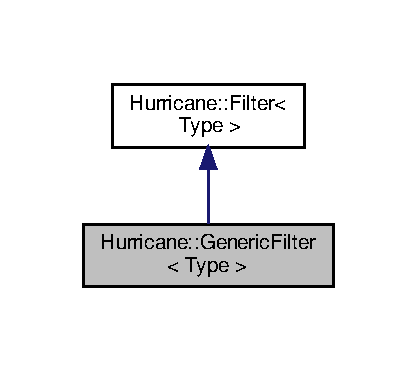
\includegraphics[width=200pt]{classHurricane_1_1GenericFilter__inherit__graph}
\end{center}
\end{figure}
\doxysubsection*{Public Member Functions}
\begin{DoxyCompactItemize}
\item 
\mbox{\hyperlink{classHurricane_1_1GenericFilter_a1aae208fe9937dd3a6f706ceb8b3b9b4}{Generic\+Filter}} (const \mbox{\hyperlink{classHurricane_1_1Filter}{Filter}}$<$ Type $>$ \&filter)
\item 
\mbox{\hyperlink{classHurricane_1_1GenericFilter_adf44866e7507f45dd0d612743f2d9a71}{Generic\+Filter}} (const \mbox{\hyperlink{classHurricane_1_1GenericFilter}{Generic\+Filter}}$<$ Type $>$ \&generic\+Filter)
\item 
\mbox{\hyperlink{classHurricane_1_1GenericFilter_aac847f0c0d6ee640c54847e374287fe1}{Generic\+Filter}} (\mbox{\hyperlink{classHurricane_1_1Filter}{Filter}}$<$ Type $>$ $\ast$filter)
\end{DoxyCompactItemize}


\doxysubsection{Detailed Description}
\subsubsection*{template$<$class Type$>$\newline
class Hurricane\+::\+Generic\+Filter$<$ Type $>$}

Generic \mbox{\hyperlink{classHurricane_1_1Filter}{Filter}} auto-\/pointer. 

This class is an auto-\/pointer like wrapped around the raw filter. The database systematically returns filters wrapped inside \mbox{\hyperlink{classHurricane_1_1GenericFilter}{Generic\+Filter}}.

\begin{DoxyRemark}{Remarks}
The destruction of a \mbox{\hyperlink{classHurricane_1_1GenericFilter}{Generic\+Filter}} triggers the destruction of the raw filter. 
\end{DoxyRemark}


\doxysubsection{Constructor \& Destructor Documentation}
\mbox{\Hypertarget{classHurricane_1_1GenericFilter_a1aae208fe9937dd3a6f706ceb8b3b9b4}\label{classHurricane_1_1GenericFilter_a1aae208fe9937dd3a6f706ceb8b3b9b4}} 
\index{Hurricane::GenericFilter$<$ Type $>$@{Hurricane::GenericFilter$<$ Type $>$}!GenericFilter@{GenericFilter}}
\index{GenericFilter@{GenericFilter}!Hurricane::GenericFilter$<$ Type $>$@{Hurricane::GenericFilter$<$ Type $>$}}
\doxysubsubsection{\texorpdfstring{GenericFilter()}{GenericFilter()}\hspace{0.1cm}{\footnotesize\ttfamily [1/3]}}
{\footnotesize\ttfamily template$<$class Type $>$ \\
\mbox{\hyperlink{classHurricane_1_1GenericFilter}{Hurricane\+::\+Generic\+Filter}}$<$ Type $>$\+::\mbox{\hyperlink{classHurricane_1_1GenericFilter}{Generic\+Filter}} (\begin{DoxyParamCaption}\item[{const \mbox{\hyperlink{classHurricane_1_1Filter}{Filter}}$<$ Type $>$ \&}]{filter }\end{DoxyParamCaption})\hspace{0.3cm}{\ttfamily [inline]}}

Constructor from a raw \mbox{\hyperlink{classHurricane_1_1Filter}{Filter}}.

\begin{DoxyRemark}{Remarks}
This constructor build a {\itshape copy} of the raw filter. So the originating filter can be safely deleted. 
\end{DoxyRemark}
\mbox{\Hypertarget{classHurricane_1_1GenericFilter_adf44866e7507f45dd0d612743f2d9a71}\label{classHurricane_1_1GenericFilter_adf44866e7507f45dd0d612743f2d9a71}} 
\index{Hurricane::GenericFilter$<$ Type $>$@{Hurricane::GenericFilter$<$ Type $>$}!GenericFilter@{GenericFilter}}
\index{GenericFilter@{GenericFilter}!Hurricane::GenericFilter$<$ Type $>$@{Hurricane::GenericFilter$<$ Type $>$}}
\doxysubsubsection{\texorpdfstring{GenericFilter()}{GenericFilter()}\hspace{0.1cm}{\footnotesize\ttfamily [2/3]}}
{\footnotesize\ttfamily template$<$class Type $>$ \\
\mbox{\hyperlink{classHurricane_1_1GenericFilter}{Hurricane\+::\+Generic\+Filter}}$<$ Type $>$\+::\mbox{\hyperlink{classHurricane_1_1GenericFilter}{Generic\+Filter}} (\begin{DoxyParamCaption}\item[{const \mbox{\hyperlink{classHurricane_1_1GenericFilter}{Generic\+Filter}}$<$ Type $>$ \&}]{filter }\end{DoxyParamCaption})\hspace{0.3cm}{\ttfamily [inline]}}

Constructor from a raw \mbox{\hyperlink{classHurricane_1_1Filter}{Filter}}.

\begin{DoxyRemark}{Remarks}
This constructor build a {\itshape copy} of the raw filter. So the originating filter can be safely deleted. 
\end{DoxyRemark}
\mbox{\Hypertarget{classHurricane_1_1GenericFilter_aac847f0c0d6ee640c54847e374287fe1}\label{classHurricane_1_1GenericFilter_aac847f0c0d6ee640c54847e374287fe1}} 
\index{Hurricane::GenericFilter$<$ Type $>$@{Hurricane::GenericFilter$<$ Type $>$}!GenericFilter@{GenericFilter}}
\index{GenericFilter@{GenericFilter}!Hurricane::GenericFilter$<$ Type $>$@{Hurricane::GenericFilter$<$ Type $>$}}
\doxysubsubsection{\texorpdfstring{GenericFilter()}{GenericFilter()}\hspace{0.1cm}{\footnotesize\ttfamily [3/3]}}
{\footnotesize\ttfamily template$<$class Type $>$ \\
\mbox{\hyperlink{classHurricane_1_1GenericFilter}{Hurricane\+::\+Generic\+Filter}}$<$ Type $>$\+::\mbox{\hyperlink{classHurricane_1_1GenericFilter}{Generic\+Filter}} (\begin{DoxyParamCaption}\item[{\mbox{\hyperlink{classHurricane_1_1Filter}{Filter}}$<$ Type $>$ $\ast$}]{filter }\end{DoxyParamCaption})\hspace{0.3cm}{\ttfamily [inline]}}

Constructor from a raw \mbox{\hyperlink{classHurricane_1_1Filter}{Filter}}.

\begin{DoxyRemark}{Remarks}
This constructor do not build a copy of the raw filter. So the original raw filter must not be deleted. It\textquotesingle{}s deletion will occurs with the one of the \mbox{\hyperlink{classHurricane_1_1GenericFilter}{Generic\+Filter}}. 
\end{DoxyRemark}


The documentation for this class was generated from the following files\+:\begin{DoxyCompactItemize}
\item 
Filter.\+h\item 
Filter.\+dox\end{DoxyCompactItemize}

\hypertarget{classHurricane_1_1GenericLocator}{}\doxysection{Hurricane\+::Generic\+Locator$<$ Type $>$ Class Template Reference}
\label{classHurricane_1_1GenericLocator}\index{Hurricane::GenericLocator$<$ Type $>$@{Hurricane::GenericLocator$<$ Type $>$}}


Generic \mbox{\hyperlink{classHurricane_1_1Locator}{Locator}} auto-\/pointer.  




Inheritance diagram for Hurricane\+::Generic\+Locator$<$ Type $>$\+:\nopagebreak
\begin{figure}[H]
\begin{center}
\leavevmode
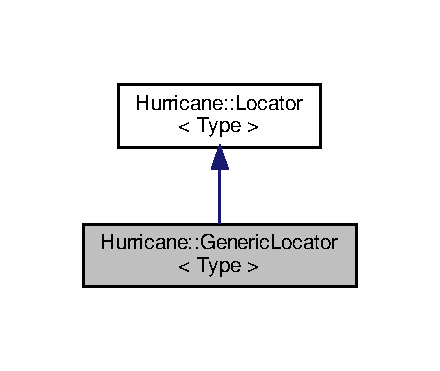
\includegraphics[width=211pt]{classHurricane_1_1GenericLocator__inherit__graph}
\end{center}
\end{figure}
\doxysubsection*{Public Member Functions}
\begin{DoxyCompactItemize}
\item 
\mbox{\hyperlink{classHurricane_1_1GenericLocator_a878eae335b3f60fc66ec6362d84c2b3e}{Generic\+Locator}} (const \mbox{\hyperlink{classHurricane_1_1Locator}{Locator}}$<$ Type $>$ \&locator)
\item 
\mbox{\hyperlink{classHurricane_1_1GenericLocator_aa314dea86573d1cee1d1eea8ac2ab49e}{Generic\+Locator}} (const \mbox{\hyperlink{classHurricane_1_1GenericLocator}{Generic\+Locator}} \&generic\+Locator)
\item 
\mbox{\hyperlink{classHurricane_1_1GenericLocator_a4706b6502b806f90f2374df76791a729}{Generic\+Locator}} (\mbox{\hyperlink{classHurricane_1_1Locator}{Locator}}$<$ Type $>$ $\ast$locator)
\end{DoxyCompactItemize}


\doxysubsection{Detailed Description}
\subsubsection*{template$<$class Type$>$\newline
class Hurricane\+::\+Generic\+Locator$<$ Type $>$}

Generic \mbox{\hyperlink{classHurricane_1_1Locator}{Locator}} auto-\/pointer. 

This class is an auto-\/pointer like wrapped around the raw locator.

\begin{DoxyRemark}{Remarks}
The destruction of a \mbox{\hyperlink{classHurricane_1_1GenericLocator}{Generic\+Locator}} triggers the destruction of the raw locator. 
\end{DoxyRemark}


\doxysubsection{Constructor \& Destructor Documentation}
\mbox{\Hypertarget{classHurricane_1_1GenericLocator_a878eae335b3f60fc66ec6362d84c2b3e}\label{classHurricane_1_1GenericLocator_a878eae335b3f60fc66ec6362d84c2b3e}} 
\index{Hurricane::GenericLocator$<$ Type $>$@{Hurricane::GenericLocator$<$ Type $>$}!GenericLocator@{GenericLocator}}
\index{GenericLocator@{GenericLocator}!Hurricane::GenericLocator$<$ Type $>$@{Hurricane::GenericLocator$<$ Type $>$}}
\doxysubsubsection{\texorpdfstring{GenericLocator()}{GenericLocator()}\hspace{0.1cm}{\footnotesize\ttfamily [1/3]}}
{\footnotesize\ttfamily template$<$class Type $>$ \\
\mbox{\hyperlink{classHurricane_1_1GenericLocator}{Hurricane\+::\+Generic\+Locator}}$<$ Type $>$\+::\mbox{\hyperlink{classHurricane_1_1GenericLocator}{Generic\+Locator}} (\begin{DoxyParamCaption}\item[{const \mbox{\hyperlink{classHurricane_1_1Locator}{Locator}}$<$ Type $>$ \&}]{locator }\end{DoxyParamCaption})\hspace{0.3cm}{\ttfamily [inline]}}

Constructor from a primary \mbox{\hyperlink{classHurricane_1_1Locator}{Locator}}.

\begin{DoxyRemark}{Remarks}
This constructor build a {\itshape copy} of the raw locator. So the originating locator can be safely deleted. 
\end{DoxyRemark}
\mbox{\Hypertarget{classHurricane_1_1GenericLocator_aa314dea86573d1cee1d1eea8ac2ab49e}\label{classHurricane_1_1GenericLocator_aa314dea86573d1cee1d1eea8ac2ab49e}} 
\index{Hurricane::GenericLocator$<$ Type $>$@{Hurricane::GenericLocator$<$ Type $>$}!GenericLocator@{GenericLocator}}
\index{GenericLocator@{GenericLocator}!Hurricane::GenericLocator$<$ Type $>$@{Hurricane::GenericLocator$<$ Type $>$}}
\doxysubsubsection{\texorpdfstring{GenericLocator()}{GenericLocator()}\hspace{0.1cm}{\footnotesize\ttfamily [2/3]}}
{\footnotesize\ttfamily template$<$class Type $>$ \\
\mbox{\hyperlink{classHurricane_1_1GenericLocator}{Hurricane\+::\+Generic\+Locator}}$<$ Type $>$\+::\mbox{\hyperlink{classHurricane_1_1GenericLocator}{Generic\+Locator}} (\begin{DoxyParamCaption}\item[{const \mbox{\hyperlink{classHurricane_1_1GenericLocator}{Generic\+Locator}}$<$ Type $>$ \&}]{generic\+Locator }\end{DoxyParamCaption})\hspace{0.3cm}{\ttfamily [inline]}}

Constructor from a primary \mbox{\hyperlink{classHurricane_1_1Locator}{Locator}} and a \mbox{\hyperlink{classHurricane_1_1Filter}{Filter}}.

\begin{DoxyRemark}{Remarks}
This constructor build a {\itshape copy} of the raw locator. So the originating locator can be safely deleted. 
\end{DoxyRemark}
\mbox{\Hypertarget{classHurricane_1_1GenericLocator_a4706b6502b806f90f2374df76791a729}\label{classHurricane_1_1GenericLocator_a4706b6502b806f90f2374df76791a729}} 
\index{Hurricane::GenericLocator$<$ Type $>$@{Hurricane::GenericLocator$<$ Type $>$}!GenericLocator@{GenericLocator}}
\index{GenericLocator@{GenericLocator}!Hurricane::GenericLocator$<$ Type $>$@{Hurricane::GenericLocator$<$ Type $>$}}
\doxysubsubsection{\texorpdfstring{GenericLocator()}{GenericLocator()}\hspace{0.1cm}{\footnotesize\ttfamily [3/3]}}
{\footnotesize\ttfamily template$<$class Type $>$ \\
\mbox{\hyperlink{classHurricane_1_1GenericLocator}{Hurricane\+::\+Generic\+Locator}}$<$ Type $>$\+::\mbox{\hyperlink{classHurricane_1_1GenericLocator}{Generic\+Locator}} (\begin{DoxyParamCaption}\item[{\mbox{\hyperlink{classHurricane_1_1Locator}{Locator}}$<$ Type $>$ $\ast$}]{locator }\end{DoxyParamCaption})\hspace{0.3cm}{\ttfamily [inline]}}

Constructor from a raw \mbox{\hyperlink{classHurricane_1_1Locator}{Locator}}.

\begin{DoxyRemark}{Remarks}
This constructor do not build a copy of the raw locator. So the original raw locator must not be deleted. It\textquotesingle{}s deletion will occurs with the one of the \mbox{\hyperlink{classHurricane_1_1GenericLocator}{Generic\+Locator}}. 
\end{DoxyRemark}


The documentation for this class was generated from the following files\+:\begin{DoxyCompactItemize}
\item 
Locator.\+h\item 
Locator.\+dox\end{DoxyCompactItemize}

\hypertarget{classHurricane_1_1Go}{}\section{Hurricane\+:\+:Go Class Reference}
\label{classHurricane_1_1Go}\index{Hurricane\+::\+Go@{Hurricane\+::\+Go}}


\mbox{\hyperlink{classHurricane_1_1Go}{Go}} description ({\bfseries A\+PI})  




Inheritance diagram for Hurricane\+:\+:Go\+:\nopagebreak
\begin{figure}[H]
\begin{center}
\leavevmode
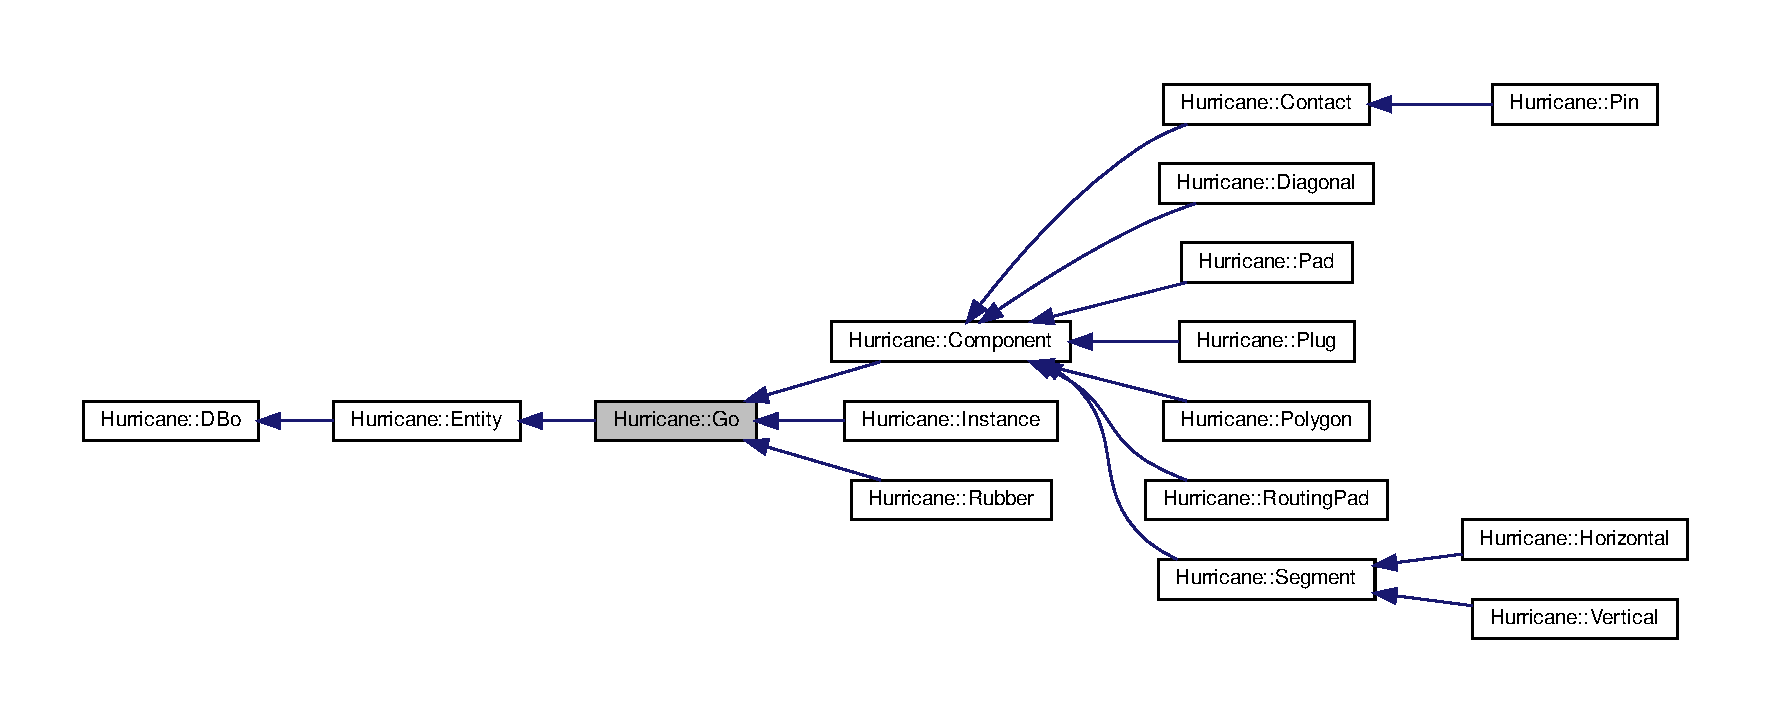
\includegraphics[width=350pt]{classHurricane_1_1Go__inherit__graph}
\end{center}
\end{figure}
\subsection*{Public Member Functions}
\begin{DoxyCompactItemize}
\item 
bool \mbox{\hyperlink{classHurricane_1_1Go_a0fd2574d3e2e0157230209acdc1b8aa6}{is\+Materialized}} () const
\item 
virtual void \mbox{\hyperlink{classHurricane_1_1Go_a8251eba8fabfca57f574921c6c85728f}{materialize}} ()=0
\item 
virtual void \mbox{\hyperlink{classHurricane_1_1Go_af79318dc9cbbed85aea1bb8f16eb9724}{unmaterialize}} ()=0
\item 
virtual void \mbox{\hyperlink{classHurricane_1_1Go_a5ee451e118fe8cace16989c0f3a6d855}{invalidate}} (bool propagate\+Flag=true)
\item 
virtual void \mbox{\hyperlink{classHurricane_1_1Go_a54c4351dbbf4045e1aa89f06bb893402}{translate}} (const \mbox{\hyperlink{group__DbUGroup_ga4fbfa3e8c89347af76c9628ea06c4146}{Db\+U\+::\+Unit}} \&dx, const \mbox{\hyperlink{group__DbUGroup_ga4fbfa3e8c89347af76c9628ea06c4146}{Db\+U\+::\+Unit}} \&dy)=0
\end{DoxyCompactItemize}
\subsection*{Static Public Member Functions}
\begin{DoxyCompactItemize}
\item 
static bool \mbox{\hyperlink{classHurricane_1_1Go_a1057be4198a7b64c32a2ac3c7d560014}{auto\+Materialization\+Is\+Disabled}} ()
\item 
static void \mbox{\hyperlink{classHurricane_1_1Go_ab0b1ca3c606247e1ebd7cab8fa828b04}{enable\+Auto\+Materialization}} ()
\item 
static void \mbox{\hyperlink{classHurricane_1_1Go_a0d49d22a3788e8001e58152e62b9f3cc}{disable\+Auto\+Materialization}} ()
\end{DoxyCompactItemize}


\subsection{Detailed Description}
\mbox{\hyperlink{classHurricane_1_1Go}{Go}} description ({\bfseries A\+PI}) 

\hypertarget{classHurricane_1_1Go_secGoIntro}{}\subsection{Introduction}\label{classHurricane_1_1Go_secGoIntro}
The Gos represent the category of graphical objects.

They are stored in a fast geometric access data structure \+: a quadtree (let us recall that the organization of each quadtree depends essentially of the geometrical envelope of those objects and of their number).\hypertarget{classHurricane_1_1Go_secGoMaterialization}{}\subsection{Materialization}\label{classHurricane_1_1Go_secGoMaterialization}
A graphical object can be materialized or not.

A graphical object is said materialized when it is effectively inserted into a quadtree. It has then a graphical appearance (it\textquotesingle{}s the least it can do) but also it will be taken into account within each collection which uses quadtrees in order to find its constituents (like the collection returned by the call cell-\/$>$Get\+Components\+Under(area) for instance).

On the other hand, non materialized graphic objects will neither be visible nor taken into account by those collections. This may be a significant advantage in some situations and a great drawback in others.

\begin{DoxyRemark}{Remarks}
{\bfseries Plugs are never materialized}.
\end{DoxyRemark}
\hypertarget{classHurricane_1_1Go_secGoUpdateSessions}{}\subsection{Update sessions}\label{classHurricane_1_1Go_secGoUpdateSessions}
The location of an object within its quadtree depends of its bounding box, if a modification of this one must occur for any reason, the object must be removed from the quadtree before doing the modification and re-\/inserted after, at the right place, according to its new bounding box.

Furthermore the change on an object may lead to changes on other ones. For instance the move of a contact will forcefully affect the components which are anchored on it, and so forth ...

Furthermore it may be interesting to apply many modifications at the same time, avoiding so intermediate or useless multiple updates (many changes on the same object but also on different objects lying in different unrelated cells).

type\+: In order to control this process we must operate in three steps

Open an update session. Do all the needed modifications. Close the update session.

type\+: Let us examine the following piece of code which illustrates that 
\begin{DoxyCode}
UpdateSession::open();
 
contact->setLayer(...);
contact->setSize(...);
contact->setPosition(...);
 
UpdateSession::close();
\end{DoxyCode}
 The call to the generic function {\bfseries Update\+Session\+::open()} allows to open a new update\+\_\+session.

The three following lines call upon functions which modify the contact and, for the last one, also the components which directly or indirectly bear on it.

At last the call to the generic function {\bfseries Update\+Session\+::close()} allows to close the last update session currently open.

type\+: What does really happen ?

The update sesion is a shared property which is put at its creation on the top of a F\+I\+FO stack. The last update cession placed on the top of this stack represents the current session.

When the object is modified \+: the method {\bfseries \mbox{\hyperlink{classHurricane_1_1Go_a5ee451e118fe8cace16989c0f3a6d855}{Go\+::invalidate()}}} which we will detail later is called upon. The purpose of this method is to de-\/materialize all materialized objects affected directly or indirectly by this modification and notify those objects to the current update session. Each of those objects then becomes an owner of this update session which is, let us recall it, a shared property.

Finally, when the current update session is closed, it is simply unstacked and destroyed. While being destroyed, it materializes again the objects which are still attached to it, that is those which were de-\/materialized within the modification phase (and only those ones) and which were not destroyed in between (invaluable contribution of the shared property).\hypertarget{classHurricane_1_1Go_secGoConstructionAndDestruction}{}\subsection{Construction and destruction}\label{classHurricane_1_1Go_secGoConstructionAndDestruction}
Graphic objects are, by default, automatically materialized at their creation (unless the plugs which are never materialized) and forcefully de-\/materialized at their destruction.

Nevertheless it is possible to inhibit temporarily the automatic materialization in some cases (like within the loading phase for instance) and to execute the materialization a posteriory and in a global way.\+This allows to avoid multiple updates of the quadtree. 

\subsection{Member Function Documentation}
\mbox{\Hypertarget{classHurricane_1_1Go_a1057be4198a7b64c32a2ac3c7d560014}\label{classHurricane_1_1Go_a1057be4198a7b64c32a2ac3c7d560014}} 
\index{Hurricane\+::\+Go@{Hurricane\+::\+Go}!auto\+Materialization\+Is\+Disabled@{auto\+Materialization\+Is\+Disabled}}
\index{auto\+Materialization\+Is\+Disabled@{auto\+Materialization\+Is\+Disabled}!Hurricane\+::\+Go@{Hurricane\+::\+Go}}
\subsubsection{\texorpdfstring{auto\+Materialization\+Is\+Disabled()}{autoMaterializationIsDisabled()}}
{\footnotesize\ttfamily bool Hurricane\+::\+Go\+::auto\+Materialization\+Is\+Disabled (\begin{DoxyParamCaption}{ }\end{DoxyParamCaption})\hspace{0.3cm}{\ttfamily [static]}}

{\bfseries Returns\+:} {\bfseries true} if the automatic materialization is disabled. \mbox{\Hypertarget{classHurricane_1_1Go_a0fd2574d3e2e0157230209acdc1b8aa6}\label{classHurricane_1_1Go_a0fd2574d3e2e0157230209acdc1b8aa6}} 
\index{Hurricane\+::\+Go@{Hurricane\+::\+Go}!is\+Materialized@{is\+Materialized}}
\index{is\+Materialized@{is\+Materialized}!Hurricane\+::\+Go@{Hurricane\+::\+Go}}
\subsubsection{\texorpdfstring{is\+Materialized()}{isMaterialized()}}
{\footnotesize\ttfamily bool Hurricane\+::\+Go\+::is\+Materialized (\begin{DoxyParamCaption}{ }\end{DoxyParamCaption}) const\hspace{0.3cm}{\ttfamily [inline]}}

{\bfseries Returns\+:} {\bfseries true} if the \mbox{\hyperlink{classHurricane_1_1Go}{Go}} is materialized, that is, inserted in the \mbox{\hyperlink{classHurricane_1_1QuadTree}{Quad\+Tree}}. \mbox{\Hypertarget{classHurricane_1_1Go_ab0b1ca3c606247e1ebd7cab8fa828b04}\label{classHurricane_1_1Go_ab0b1ca3c606247e1ebd7cab8fa828b04}} 
\index{Hurricane\+::\+Go@{Hurricane\+::\+Go}!enable\+Auto\+Materialization@{enable\+Auto\+Materialization}}
\index{enable\+Auto\+Materialization@{enable\+Auto\+Materialization}!Hurricane\+::\+Go@{Hurricane\+::\+Go}}
\subsubsection{\texorpdfstring{enable\+Auto\+Materialization()}{enableAutoMaterialization()}}
{\footnotesize\ttfamily void Hurricane\+::\+Go\+::enable\+Auto\+Materialization (\begin{DoxyParamCaption}{ }\end{DoxyParamCaption})\hspace{0.3cm}{\ttfamily [static]}}

\begin{DoxySeeAlso}{See also}
Go\+::\+Disable\+Auto\+Materialization(). 
\end{DoxySeeAlso}
\mbox{\Hypertarget{classHurricane_1_1Go_a0d49d22a3788e8001e58152e62b9f3cc}\label{classHurricane_1_1Go_a0d49d22a3788e8001e58152e62b9f3cc}} 
\index{Hurricane\+::\+Go@{Hurricane\+::\+Go}!disable\+Auto\+Materialization@{disable\+Auto\+Materialization}}
\index{disable\+Auto\+Materialization@{disable\+Auto\+Materialization}!Hurricane\+::\+Go@{Hurricane\+::\+Go}}
\subsubsection{\texorpdfstring{disable\+Auto\+Materialization()}{disableAutoMaterialization()}}
{\footnotesize\ttfamily void Hurricane\+::\+Go\+::disable\+Auto\+Materialization (\begin{DoxyParamCaption}{ }\end{DoxyParamCaption})\hspace{0.3cm}{\ttfamily [static]}}

Those two static member functions allows to inhibit or restore the automatic materialization of all graphic objects.

When the automatic materialization is inhibited, the postponed materialization of dematerialized objects has to be taken in charge explicitely by the developper (it will not be automatically done at the restore of the automatic mode).

The following sample code shows how to proceed \+: 
\begin{DoxyCode}
Cell* LoadCellFromFile ( ... )
\{
   Cell* cell = \mbox{\hyperlink{classHurricane_1_1Cell_ad803afb3e52bea3bf3d520e353b162e0}{Cell::create}}( ... );
 
   \textcolor{keywordtype}{bool} enabledFlag = not \mbox{\hyperlink{classHurricane_1_1Go_a1057be4198a7b64c32a2ac3c7d560014}{Go::autoMaterializationIsDisabled}}();
   \mbox{\hyperlink{classHurricane_1_1Go_a0d49d22a3788e8001e58152e62b9f3cc}{Go::disableAutoMaterialization}}(); \textcolor{comment}{// we force the mode}
 
   ... \textcolor{comment}{// we open the file and load the cell }
 
   \textcolor{keywordflow}{if} (enabledFlag) \textcolor{comment}{// we restore the initial state if needed}
     \mbox{\hyperlink{classHurricane_1_1Go_ab0b1ca3c606247e1ebd7cab8fa828b04}{Go::enableAutoMaterialization}}();
 
   cell->materialize(); \textcolor{comment}{// delayed materialization of cell content}
 
   \textcolor{keywordflow}{return} cell;
\}
\end{DoxyCode}
 \mbox{\Hypertarget{classHurricane_1_1Go_a8251eba8fabfca57f574921c6c85728f}\label{classHurricane_1_1Go_a8251eba8fabfca57f574921c6c85728f}} 
\index{Hurricane\+::\+Go@{Hurricane\+::\+Go}!materialize@{materialize}}
\index{materialize@{materialize}!Hurricane\+::\+Go@{Hurricane\+::\+Go}}
\subsubsection{\texorpdfstring{materialize()}{materialize()}}
{\footnotesize\ttfamily void Hurricane\+::\+Go\+::materialize (\begin{DoxyParamCaption}{ }\end{DoxyParamCaption})\hspace{0.3cm}{\ttfamily [pure virtual]}}

Triggers the materialization, that is, insert into the relevant \mbox{\hyperlink{classHurricane_1_1QuadTree}{Quad\+Tree}}. \mbox{\Hypertarget{classHurricane_1_1Go_af79318dc9cbbed85aea1bb8f16eb9724}\label{classHurricane_1_1Go_af79318dc9cbbed85aea1bb8f16eb9724}} 
\index{Hurricane\+::\+Go@{Hurricane\+::\+Go}!unmaterialize@{unmaterialize}}
\index{unmaterialize@{unmaterialize}!Hurricane\+::\+Go@{Hurricane\+::\+Go}}
\subsubsection{\texorpdfstring{unmaterialize()}{unmaterialize()}}
{\footnotesize\ttfamily void Hurricane\+::\+Go\+::unmaterialize (\begin{DoxyParamCaption}{ }\end{DoxyParamCaption})\hspace{0.3cm}{\ttfamily [pure virtual]}}

Withdrawn the \mbox{\hyperlink{classHurricane_1_1Go}{Go}} from it\textquotesingle{}s \mbox{\hyperlink{classHurricane_1_1QuadTree}{Quad\+Tree}}. \mbox{\Hypertarget{classHurricane_1_1Go_a5ee451e118fe8cace16989c0f3a6d855}\label{classHurricane_1_1Go_a5ee451e118fe8cace16989c0f3a6d855}} 
\index{Hurricane\+::\+Go@{Hurricane\+::\+Go}!invalidate@{invalidate}}
\index{invalidate@{invalidate}!Hurricane\+::\+Go@{Hurricane\+::\+Go}}
\subsubsection{\texorpdfstring{invalidate()}{invalidate()}}
{\footnotesize\ttfamily void Hurricane\+::\+Go\+::invalidate (\begin{DoxyParamCaption}\item[{bool}]{propagate\+Flag = {\ttfamily true} }\end{DoxyParamCaption})\hspace{0.3cm}{\ttfamily [virtual]}}

This method must be called before a change of the object geometry.

It is within this function that the object captures or not the current update session, which involves its future re-\/materialization when the time commes.

It is also within this function that all objects, whose geometry will be affected directly or indirectly by the object change, must be invalidated. The flag {\ttfamily $<$propagate\+Flag$>$} allows to limit the propagation in some cases (i.\+e. when the contact size changes, objects anchored on it are not affected and there is no need to invalidate them).

An already dematerialized object must not be taken in count in the current update session, but its propagation, if required, must be systematically executed.

\begin{DoxyParagraph}{Sample\+: We give as an example the implementation for the instances \+:}

\begin{DoxyCode}
\textcolor{keywordtype}{void} Instance::invalidate ( \textcolor{keywordtype}{bool} propagateFlag )
\{
  Inherit::invalidate(\textcolor{keyword}{false});
 
  \textcolor{keywordflow}{if} (propagateFlag) \{
    forEach(Plug*, iplug, GetConnectedPlugs()) \{
      iplug->invalidate(\textcolor{keyword}{true});
    \}
  \}
\}
\end{DoxyCode}
 
\begin{DoxyCode}
\textcolor{keywordtype}{void} Component::invalidate ( \textcolor{keywordtype}{bool} propagateFlag )
\{
  Inherit::invalidate(\textcolor{keyword}{false});
 
  \textcolor{keywordflow}{if} (propagateFlag) \{
    forEach(Component*, icomponent, GetSlaveComponents()) \{
      icomponent->invalidate(\textcolor{keyword}{false});
    \}
  \}
\}
\end{DoxyCode}
 
\begin{DoxyCode}
\textcolor{keywordtype}{void} \mbox{\hyperlink{classHurricane_1_1Contact_aec627634d5b6cfc5079a02b1b518b50e}{Contact::setLayer}} ( Layer* layer )
\{
  \textcolor{keywordflow}{if} (!layer) \textcolor{keywordflow}{throw} Error(\textcolor{stringliteral}{"Can't set layer : null layer"});
 
  \textcolor{keywordflow}{if} (layer != \_layer) \{
    \textcolor{comment}{// we do the change only if necessary}
    \mbox{\hyperlink{classHurricane_1_1Go_a5ee451e118fe8cace16989c0f3a6d855}{invalidate}}(\textcolor{keyword}{false}); \textcolor{comment}{// done before the modification}
 
    \_layer = layer;
  \}
\}
\end{DoxyCode}
 
\begin{DoxyCode}
\textcolor{keywordtype}{void} \mbox{\hyperlink{classHurricane_1_1Instance_a8890d2e1b2ba2542997454297e63512f}{Instance::setTransformation}}(\textcolor{keyword}{const} Transformation& transformation)
\{
  \textcolor{keywordflow}{if} (transformation != \_transformation) \{
    \textcolor{comment}{// we do the change only if necessary}
    \mbox{\hyperlink{classHurricane_1_1Go_a5ee451e118fe8cace16989c0f3a6d855}{invalidate}}(\textcolor{keyword}{true}); \textcolor{comment}{// done before the modification}

    \_transformation = transformation;
  \}
\}
\end{DoxyCode}
 
\end{DoxyParagraph}
\mbox{\Hypertarget{classHurricane_1_1Go_a54c4351dbbf4045e1aa89f06bb893402}\label{classHurricane_1_1Go_a54c4351dbbf4045e1aa89f06bb893402}} 
\index{Hurricane\+::\+Go@{Hurricane\+::\+Go}!translate@{translate}}
\index{translate@{translate}!Hurricane\+::\+Go@{Hurricane\+::\+Go}}
\subsubsection{\texorpdfstring{translate()}{translate()}}
{\footnotesize\ttfamily void Hurricane\+::\+Go\+::translate (\begin{DoxyParamCaption}\item[{const \mbox{\hyperlink{group__DbUGroup_ga4fbfa3e8c89347af76c9628ea06c4146}{Db\+U\+::\+Unit}} \&}]{dx,  }\item[{const \mbox{\hyperlink{group__DbUGroup_ga4fbfa3e8c89347af76c9628ea06c4146}{Db\+U\+::\+Unit}} \&}]{dy }\end{DoxyParamCaption})\hspace{0.3cm}{\ttfamily [pure virtual]}}

Translate the graphic object of the quantity {\ttfamily $<$dx$>$} and {\ttfamily $<$dy$>$}.

This virtual method should be specialized for a new kind of graphic object. 

Implemented in \mbox{\hyperlink{classHurricane_1_1RoutingPad_a41bf66ffda0c0ceaaebc67acd72d5b36}{Hurricane\+::\+Routing\+Pad}}.



The documentation for this class was generated from the following files\+:\begin{DoxyCompactItemize}
\item 
Go.\+h\item 
Go.\+dox\end{DoxyCompactItemize}

\hypertarget{classHurricane_1_1Hook}{}\doxysection{Hurricane\+::Hook Class Reference}
\label{classHurricane_1_1Hook}\index{Hurricane::Hook@{Hurricane::Hook}}


\mbox{\hyperlink{classHurricane_1_1Hook}{Hook}} description ({\bfseries{API}})  




Inheritance diagram for Hurricane\+::Hook\+:\nopagebreak
\begin{figure}[H]
\begin{center}
\leavevmode
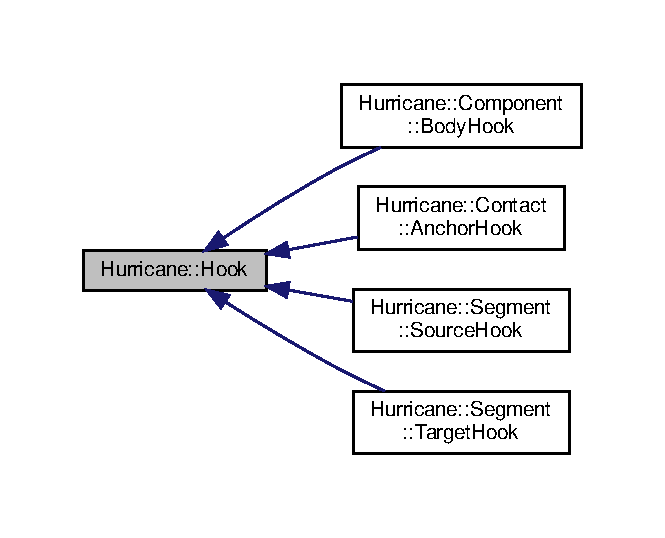
\includegraphics[width=319pt]{classHurricane_1_1Hook__inherit__graph}
\end{center}
\end{figure}
\doxysubsection*{Public Member Functions}
\begin{DoxyCompactItemize}
\item 
virtual \mbox{\hyperlink{classHurricane_1_1Component}{Component}} $\ast$ \mbox{\hyperlink{classHurricane_1_1Hook_ab420305aa59b8ff10d59678363de2511}{get\+Component}} () const =0
\item 
\mbox{\hyperlink{classHurricane_1_1Hook}{Hook}} $\ast$ \mbox{\hyperlink{classHurricane_1_1Hook_a03044fa995d6d784d6c441927ca8af04}{get\+Next\+Hook}} () const
\item 
\mbox{\hyperlink{classHurricane_1_1Hook}{Hook}} $\ast$ \mbox{\hyperlink{classHurricane_1_1Hook_ad69ebbbf3d64343aca23ca435f24c624}{get\+Previous\+Hook}} () const
\item 
\mbox{\hyperlink{classHurricane_1_1Hook}{Hook}} $\ast$ \mbox{\hyperlink{classHurricane_1_1Hook_af18e0531df4ed14b64cf058b780aee46}{get\+Master\+Hook}} () const
\item 
\mbox{\hyperlink{classHurricane_1_1Hook}{Hook}} $\ast$ \mbox{\hyperlink{classHurricane_1_1Hook_a0923a5a2d0a7ee0458876eed72008e46}{get\+Next\+Master\+Hook}} () const
\item 
\mbox{\hyperlink{classHurricane_1_1Hook}{Hook}} $\ast$ \mbox{\hyperlink{classHurricane_1_1Hook_a80bf5cdd4e81952064f1be94fe10188f}{get\+Previous\+Master\+Hook}} () const
\item 
\mbox{\hyperlink{namespaceHurricane_a9dcd9b74dc5e2b51bec7a13c25807e02}{Hooks}} \mbox{\hyperlink{classHurricane_1_1Hook_a2def96fbcd444bebc16e589357c2a779}{get\+Hooks}} () const
\item 
\mbox{\hyperlink{namespaceHurricane_a9dcd9b74dc5e2b51bec7a13c25807e02}{Hooks}} \mbox{\hyperlink{classHurricane_1_1Hook_ad3c977e4f253a18cf24dfe4a6fd24cb1}{get\+Slave\+Hooks}} () const
\item 
virtual bool \mbox{\hyperlink{classHurricane_1_1Hook_af0940eb0761f05df0b82c4198e22a01c}{is\+Master}} () const =0
\item 
bool \mbox{\hyperlink{classHurricane_1_1Hook_acd62c7de2c023a1013d5a728159d068d}{is\+Attached}} () const
\item 
\mbox{\hyperlink{classHurricane_1_1Hook}{Hook}} $\ast$ \mbox{\hyperlink{classHurricane_1_1Hook_a83f5beb5092e97947d24bd18adb33db1}{detach}} ()
\item 
\mbox{\hyperlink{classHurricane_1_1Hook}{Hook}} $\ast$ \mbox{\hyperlink{classHurricane_1_1Hook_aacc4dacd0d128b35fd15546bc6dde3c3}{attach}} (\mbox{\hyperlink{classHurricane_1_1Hook}{Hook}} $\ast$hook)
\item 
\mbox{\hyperlink{classHurricane_1_1Hook}{Hook}} $\ast$ \mbox{\hyperlink{classHurricane_1_1Hook_a7b98f0796a9080495472d574a23bcca0}{merge}} (\mbox{\hyperlink{classHurricane_1_1Hook}{Hook}} $\ast$hook)
\end{DoxyCompactItemize}


\doxysubsection{Detailed Description}
\mbox{\hyperlink{classHurricane_1_1Hook}{Hook}} description ({\bfseries{API}}) 

\hypertarget{classHurricane_1_1Hook_secHookIntro}{}\doxysubsection{Introduction}\label{classHurricane_1_1Hook_secHookIntro}
The hook is an object which is nested inside a component and which represents some specific part of this component (like its body, its origin or its extremity ...).

The \mbox{\hyperlink{classHurricane_1_1Hook}{Hook}} class is an abstract one, that means that for any new type of {\bfseries{part}} a new hook subclass must be derived. Each hook specialization will be described altogether with the component which includes it.

The \mbox{\hyperlink{classHurricane_1_1Component}{Component}} for instance introduces the concept of {\bfseries{Body\+Hook}} representing the body of the component (which can be assimilated to the component itself).\hypertarget{classHurricane_1_1Hook_secHookRings}{}\doxysubsection{Rings}\label{classHurricane_1_1Hook_secHookRings}
Hooks are assembled into a {\bfseries{ring}} (circular link) thanks to a special field pointing to the next hook within the ring.

This field is never NULL, by default it points to itself, generating a minimal ring.\hypertarget{classHurricane_1_1Hook_secHookMasterAndSlaveHookTypes}{}\doxysubsection{Master and Slave hook types}\label{classHurricane_1_1Hook_secHookMasterAndSlaveHookTypes}
There are two kinds of hooks \+: the {\bfseries{masters}} and the {\bfseries{slaves}}.

Rings are organized such that all slave hooks of a master hook are placed in the ring immediately before it (the ordering of slaves is not significant).

Therefore, to find the master of a given slave, it\textquotesingle{}s enough to follow the ring pointers, starting from the slave, until a master is found.\hypertarget{classHurricane_1_1Hook_secHookExplicitConnections}{}\doxysubsection{Explicit connections}\label{classHurricane_1_1Hook_secHookExplicitConnections}
This dependency between a slave and its master means that the part of the component represented by the slave is anchored on the part of the component represented by the master.

This dependence relationship is indeed an explicit connection.\hypertarget{classHurricane_1_1Hook_secHookImplicitConnections}{}\doxysubsection{Implicit connections}\label{classHurricane_1_1Hook_secHookImplicitConnections}
Within a ring many relationships master-\/slaves can cohabit.

This cohabitation has a specific meaning for the different masters of the ring. In fact, the ring must be considered as a connection request between the different masters of the ring.

In other words, this means that the different masters remains to be connected together, or more generaly stated, that the different connected subsets of components associated to those masters remains to be connected together.

The ordering of masters within a ring has no particular signification.\hypertarget{classHurricane_1_1Hook_secHookConceptsOfHyperhooksAndHyperrings}{}\doxysubsection{Concepts of Hyper\+Hooks and Hyper\+Rings}\label{classHurricane_1_1Hook_secHookConceptsOfHyperhooksAndHyperrings}
We can imagine the master-\/slaves relation as a kind of hyper-\/hook representing the associated sub-\/ring, and the ring containing multiple master-\/slaves relations as an hyper-\/ring made up of hyper-\/hooks needing to be connected.

Therefore there will be two different levels of ring processing functions depending on wether we handle hooks stricktly speaking or we handle hyper-\/hooks representing multiple master hooks.\hypertarget{classHurricane_1_1Hook_secHookConstructorAndDestructor}{}\doxysubsection{Constructor and Destructor}\label{classHurricane_1_1Hook_secHookConstructorAndDestructor}
There is no \mbox{\hyperlink{classHurricane_1_1Hook}{Hook}} constructor available because they are created by the components themselves.

On the same way, hooks disapear automatically with their owner. 

\doxysubsection{Member Function Documentation}
\mbox{\Hypertarget{classHurricane_1_1Hook_ab420305aa59b8ff10d59678363de2511}\label{classHurricane_1_1Hook_ab420305aa59b8ff10d59678363de2511}} 
\index{Hurricane::Hook@{Hurricane::Hook}!getComponent@{getComponent}}
\index{getComponent@{getComponent}!Hurricane::Hook@{Hurricane::Hook}}
\doxysubsubsection{\texorpdfstring{getComponent()}{getComponent()}}
{\footnotesize\ttfamily \mbox{\hyperlink{classHurricane_1_1Component}{Component}} $\ast$ Hurricane\+::\+Hook\+::get\+Component (\begin{DoxyParamCaption}{ }\end{DoxyParamCaption}) const\hspace{0.3cm}{\ttfamily [pure virtual]}}

{\bfseries{Returns\+:}} the component whose hook represents a part.

\begin{DoxyRemark}{Remarks}
The result is never NULL because hooks are byforce nested objects in their component. 
\end{DoxyRemark}
\mbox{\Hypertarget{classHurricane_1_1Hook_a03044fa995d6d784d6c441927ca8af04}\label{classHurricane_1_1Hook_a03044fa995d6d784d6c441927ca8af04}} 
\index{Hurricane::Hook@{Hurricane::Hook}!getNextHook@{getNextHook}}
\index{getNextHook@{getNextHook}!Hurricane::Hook@{Hurricane::Hook}}
\doxysubsubsection{\texorpdfstring{getNextHook()}{getNextHook()}}
{\footnotesize\ttfamily \mbox{\hyperlink{classHurricane_1_1Hook}{Hook}} $\ast$ Hurricane\+::\+Hook\+::get\+Next\+Hook (\begin{DoxyParamCaption}{ }\end{DoxyParamCaption}) const}

{\bfseries{Returns\+:}} the next hook within the ring.

\begin{DoxyRemark}{Remarks}
The result is never NULL because every hook has by construction its next one (which may be itself is the ring is empty). 
\end{DoxyRemark}
\mbox{\Hypertarget{classHurricane_1_1Hook_ad69ebbbf3d64343aca23ca435f24c624}\label{classHurricane_1_1Hook_ad69ebbbf3d64343aca23ca435f24c624}} 
\index{Hurricane::Hook@{Hurricane::Hook}!getPreviousHook@{getPreviousHook}}
\index{getPreviousHook@{getPreviousHook}!Hurricane::Hook@{Hurricane::Hook}}
\doxysubsubsection{\texorpdfstring{getPreviousHook()}{getPreviousHook()}}
{\footnotesize\ttfamily \mbox{\hyperlink{classHurricane_1_1Hook}{Hook}} $\ast$ Hurricane\+::\+Hook\+::get\+Previous\+Hook (\begin{DoxyParamCaption}{ }\end{DoxyParamCaption}) const}

{\bfseries{Returns\+:}} the previous hook within the ring.

\begin{DoxyRemark}{Remarks}
Less efficient than get\+Next\+Hook because it requires a complete ring loop. 
\end{DoxyRemark}
\mbox{\Hypertarget{classHurricane_1_1Hook_af18e0531df4ed14b64cf058b780aee46}\label{classHurricane_1_1Hook_af18e0531df4ed14b64cf058b780aee46}} 
\index{Hurricane::Hook@{Hurricane::Hook}!getMasterHook@{getMasterHook}}
\index{getMasterHook@{getMasterHook}!Hurricane::Hook@{Hurricane::Hook}}
\doxysubsubsection{\texorpdfstring{getMasterHook()}{getMasterHook()}}
{\footnotesize\ttfamily \mbox{\hyperlink{classHurricane_1_1Hook}{Hook}} $\ast$ Hurricane\+::\+Hook\+::get\+Master\+Hook (\begin{DoxyParamCaption}{ }\end{DoxyParamCaption}) const}

{\bfseries{Returns\+:}} the master of the relation master-\/slaves identified by the hook.

\begin{DoxyRemark}{Remarks}
May return itself if the hook is a master and return NULL if the hook is a slave and has no associated master. 
\end{DoxyRemark}
\mbox{\Hypertarget{classHurricane_1_1Hook_a0923a5a2d0a7ee0458876eed72008e46}\label{classHurricane_1_1Hook_a0923a5a2d0a7ee0458876eed72008e46}} 
\index{Hurricane::Hook@{Hurricane::Hook}!getNextMasterHook@{getNextMasterHook}}
\index{getNextMasterHook@{getNextMasterHook}!Hurricane::Hook@{Hurricane::Hook}}
\doxysubsubsection{\texorpdfstring{getNextMasterHook()}{getNextMasterHook()}}
{\footnotesize\ttfamily \mbox{\hyperlink{classHurricane_1_1Hook}{Hook}} $\ast$ Hurricane\+::\+Hook\+::get\+Next\+Master\+Hook (\begin{DoxyParamCaption}{ }\end{DoxyParamCaption}) const}

{\bfseries{Returns\+:}} the first master found when starting the search immediately after the given hook.

\begin{DoxyRemark}{Remarks}
May return NULL if there is no master within the ring or return the hook itself if it is a master and the only one in the ring. 
\end{DoxyRemark}
\mbox{\Hypertarget{classHurricane_1_1Hook_a80bf5cdd4e81952064f1be94fe10188f}\label{classHurricane_1_1Hook_a80bf5cdd4e81952064f1be94fe10188f}} 
\index{Hurricane::Hook@{Hurricane::Hook}!getPreviousMasterHook@{getPreviousMasterHook}}
\index{getPreviousMasterHook@{getPreviousMasterHook}!Hurricane::Hook@{Hurricane::Hook}}
\doxysubsubsection{\texorpdfstring{getPreviousMasterHook()}{getPreviousMasterHook()}}
{\footnotesize\ttfamily \mbox{\hyperlink{classHurricane_1_1Hook}{Hook}} $\ast$ Hurricane\+::\+Hook\+::get\+Previous\+Master\+Hook (\begin{DoxyParamCaption}{ }\end{DoxyParamCaption}) const}

{\bfseries{Returns\+:}} the first master found when starting a backwards search immediately before the given hook.

\begin{DoxyRemark}{Remarks}
May return NULL if there is no master within the ring or return the hook itself if it is a master and the only one in the ring.

Of course the search is done in the natural forward direction (else it would be trully inefficient). 
\end{DoxyRemark}
\mbox{\Hypertarget{classHurricane_1_1Hook_a2def96fbcd444bebc16e589357c2a779}\label{classHurricane_1_1Hook_a2def96fbcd444bebc16e589357c2a779}} 
\index{Hurricane::Hook@{Hurricane::Hook}!getHooks@{getHooks}}
\index{getHooks@{getHooks}!Hurricane::Hook@{Hurricane::Hook}}
\doxysubsubsection{\texorpdfstring{getHooks()}{getHooks()}}
{\footnotesize\ttfamily \mbox{\hyperlink{namespaceHurricane_a9dcd9b74dc5e2b51bec7a13c25807e02}{Hooks}} Hurricane\+::\+Hook\+::get\+Hooks (\begin{DoxyParamCaption}{ }\end{DoxyParamCaption}) const}

{\bfseries{Returns\+:}} the collection of hooks of the ring containing the given hook.

\begin{DoxyRemark}{Remarks}
Hooks are always visited in the natural order starting from the hook itself. 
\end{DoxyRemark}
\mbox{\Hypertarget{classHurricane_1_1Hook_ad3c977e4f253a18cf24dfe4a6fd24cb1}\label{classHurricane_1_1Hook_ad3c977e4f253a18cf24dfe4a6fd24cb1}} 
\index{Hurricane::Hook@{Hurricane::Hook}!getSlaveHooks@{getSlaveHooks}}
\index{getSlaveHooks@{getSlaveHooks}!Hurricane::Hook@{Hurricane::Hook}}
\doxysubsubsection{\texorpdfstring{getSlaveHooks()}{getSlaveHooks()}}
{\footnotesize\ttfamily \mbox{\hyperlink{namespaceHurricane_a9dcd9b74dc5e2b51bec7a13c25807e02}{Hooks}} Hurricane\+::\+Hook\+::get\+Slave\+Hooks (\begin{DoxyParamCaption}{ }\end{DoxyParamCaption}) const}

{\bfseries{Returns\+:}} the hook collection which are slaves of the given hook.

\begin{DoxyRemark}{Remarks}
This collection will be empty if the given hook is not a master or if it has no attached slaves.
\end{DoxyRemark}
When visiting the slaves of a master, those are accessed in the assembly order \+: the first one is the oldest inserted (they are accessed starting from the first slave found when starting a ring loop from the master itself).

The master is not included in this collection. \mbox{\Hypertarget{classHurricane_1_1Hook_af0940eb0761f05df0b82c4198e22a01c}\label{classHurricane_1_1Hook_af0940eb0761f05df0b82c4198e22a01c}} 
\index{Hurricane::Hook@{Hurricane::Hook}!isMaster@{isMaster}}
\index{isMaster@{isMaster}!Hurricane::Hook@{Hurricane::Hook}}
\doxysubsubsection{\texorpdfstring{isMaster()}{isMaster()}}
{\footnotesize\ttfamily bool Hurricane\+::\+Hook\+::is\+Master (\begin{DoxyParamCaption}{ }\end{DoxyParamCaption}) const\hspace{0.3cm}{\ttfamily [pure virtual]}}

{\bfseries{Returns\+:}} {\bfseries{true}} if the hook must be considered as a master, else {\bfseries{false}}.

\begin{DoxyRemark}{Remarks}
For any new kind of hook this predicate must be overloaded. 
\end{DoxyRemark}
\mbox{\Hypertarget{classHurricane_1_1Hook_acd62c7de2c023a1013d5a728159d068d}\label{classHurricane_1_1Hook_acd62c7de2c023a1013d5a728159d068d}} 
\index{Hurricane::Hook@{Hurricane::Hook}!isAttached@{isAttached}}
\index{isAttached@{isAttached}!Hurricane::Hook@{Hurricane::Hook}}
\doxysubsubsection{\texorpdfstring{isAttached()}{isAttached()}}
{\footnotesize\ttfamily bool Hurricane\+::\+Hook\+::is\+Attached (\begin{DoxyParamCaption}{ }\end{DoxyParamCaption}) const}

If the hook is a slave \+:

{\bfseries{Returns\+:}} {\bfseries{true}} if the hook has an associated master, else {\bfseries{false}}.

\begin{DoxyRemark}{Remarks}
You can\textquotesingle{}t find two slaves in the same ring without at least a master.
\end{DoxyRemark}
If the hook is a master \+:

Let us consider the hyper-\/ring made upon hyper-\/hooks. Then the function returns {\bfseries{true}} if the ring contains at least an other master else {\bfseries{false}}.

\begin{DoxyParagraph}{Caution\+: The meaning here is very different than for a slave hook! }

\end{DoxyParagraph}
\mbox{\Hypertarget{classHurricane_1_1Hook_a83f5beb5092e97947d24bd18adb33db1}\label{classHurricane_1_1Hook_a83f5beb5092e97947d24bd18adb33db1}} 
\index{Hurricane::Hook@{Hurricane::Hook}!detach@{detach}}
\index{detach@{detach}!Hurricane::Hook@{Hurricane::Hook}}
\doxysubsubsection{\texorpdfstring{detach()}{detach()}}
{\footnotesize\ttfamily \mbox{\hyperlink{classHurricane_1_1Hook}{Hook}} $\ast$ Hurricane\+::\+Hook\+::detach (\begin{DoxyParamCaption}{ }\end{DoxyParamCaption})}

If the hook is a slave \+:

detaches the hook from its ring and returns its old predecessor.

\begin{DoxyRemark}{Remarks}
Will return NULL if the hook is the only one in the ring.
\end{DoxyRemark}
If the hook is a master \+:

Let us consider the hyper-\/ring made upon hyper-\/hooks. Then, the function detaches the hyper-\/hook (the sub-\/ring made up of the master and its slaves, if any) from the hyper-\/ring and returns the old predecessor of the hyper-\/hook.

Within the detached hyper-\/hook, the relationship master hook
\begin{DoxyItemize}
\item slave hooks remains unaltered and forms a new ring.
\end{DoxyItemize}

\begin{DoxyRemark}{Remarks}
May return NULL if the hook is the only master of the ring.
\end{DoxyRemark}
The returned hook, if not NULL, is byforce a master. \mbox{\Hypertarget{classHurricane_1_1Hook_aacc4dacd0d128b35fd15546bc6dde3c3}\label{classHurricane_1_1Hook_aacc4dacd0d128b35fd15546bc6dde3c3}} 
\index{Hurricane::Hook@{Hurricane::Hook}!attach@{attach}}
\index{attach@{attach}!Hurricane::Hook@{Hurricane::Hook}}
\doxysubsubsection{\texorpdfstring{attach()}{attach()}}
{\footnotesize\ttfamily \mbox{\hyperlink{classHurricane_1_1Hook}{Hook}} $\ast$ Hurricane\+::\+Hook\+::attach (\begin{DoxyParamCaption}\item[{\mbox{\hyperlink{classHurricane_1_1Hook}{Hook}} $\ast$}]{master\+Hook }\end{DoxyParamCaption})}

If the hook (this) is a slave \+:

The function inserts the hook immediately before {\ttfamily $<$master\+Hook$>$} and returns this master\+Hook.

\begin{DoxyParagraph}{Caution\+: Might throw an exception if the hook already has a master or }
if {\ttfamily $<$master\+Hook$>$} is not a master hook.
\end{DoxyParagraph}
If the hook (this) is a master \+:

Let us consider the hyper-\/ring made upon hyper-\/hooks. Then, the function attaches the the hyper-\/hook (the sub-\/ring made up of this master hook and its slaves, if any) before the {\ttfamily $<$master\+Hook$>$} and returns this master\+Hook.

\begin{DoxyParagraph}{Caution\+: Might throw an exception if the hyper-\/hook is already }
attached within a ring including an other master or if {\ttfamily $<$master\+Hook$>$} is not a master hook. 
\end{DoxyParagraph}
\mbox{\Hypertarget{classHurricane_1_1Hook_a7b98f0796a9080495472d574a23bcca0}\label{classHurricane_1_1Hook_a7b98f0796a9080495472d574a23bcca0}} 
\index{Hurricane::Hook@{Hurricane::Hook}!merge@{merge}}
\index{merge@{merge}!Hurricane::Hook@{Hurricane::Hook}}
\doxysubsubsection{\texorpdfstring{merge()}{merge()}}
{\footnotesize\ttfamily \mbox{\hyperlink{classHurricane_1_1Hook}{Hook}} $\ast$ Hurricane\+::\+Hook\+::merge (\begin{DoxyParamCaption}\item[{\mbox{\hyperlink{classHurricane_1_1Hook}{Hook}} $\ast$}]{master\+Hook }\end{DoxyParamCaption})}

merges the rings represented by the two hooks which both must be masters, returns {\ttfamily $<$master\+Hook$>$}.

\begin{DoxyRemark}{Remarks}
Throws an exception if both hooks are not masters.
\end{DoxyRemark}
This function doesn\textquotesingle{}t change the two relatioships master-\/slaves but modifies the connection request between corresponding hyper-\/hooks. 

The documentation for this class was generated from the following files\+:\begin{DoxyCompactItemize}
\item 
Hook.\+h\item 
Hook.\+dox\end{DoxyCompactItemize}

\hypertarget{classHurricane_1_1Horizontal}{}\doxysection{Hurricane\+::Horizontal Class Reference}
\label{classHurricane_1_1Horizontal}\index{Hurricane::Horizontal@{Hurricane::Horizontal}}


\mbox{\hyperlink{classHurricane_1_1Horizontal}{Horizontal}} description ({\bfseries{API}})  




Inheritance diagram for Hurricane\+::Horizontal\+:\nopagebreak
\begin{figure}[H]
\begin{center}
\leavevmode
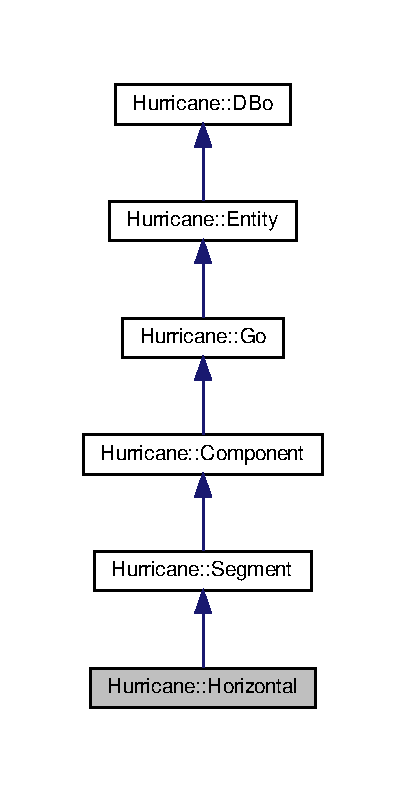
\includegraphics[width=195pt]{classHurricane_1_1Horizontal__inherit__graph}
\end{center}
\end{figure}
\doxysubsection*{Public Types}
\begin{DoxyCompactItemize}
\item 
typedef \mbox{\hyperlink{classHurricane_1_1Segment}{Segment}} \mbox{\hyperlink{classHurricane_1_1Horizontal_a43266e3530dc5872f4eabf16eba86bdb}{Inherit}}
\end{DoxyCompactItemize}
\doxysubsection*{Public Member Functions}
\begin{DoxyCompactItemize}
\item 
const \mbox{\hyperlink{classHurricane_1_1DbU_a4fbfa3e8c89347af76c9628ea06c4146}{Db\+U\+::\+Unit}} \& \mbox{\hyperlink{classHurricane_1_1Horizontal_a7fdafaa2a7e931413efb2c1fc021f4a8}{get\+Dx\+Source}} () const
\item 
const \mbox{\hyperlink{classHurricane_1_1DbU_a4fbfa3e8c89347af76c9628ea06c4146}{Db\+U\+::\+Unit}} \& \mbox{\hyperlink{classHurricane_1_1Horizontal_aab807785755e4229f215aee3f3b16941}{get\+Dx\+Target}} () const
\item 
void \mbox{\hyperlink{classHurricane_1_1Horizontal_a794aa68157beb2d04816a5f4e9160187}{setY}} (const \mbox{\hyperlink{classHurricane_1_1DbU_a4fbfa3e8c89347af76c9628ea06c4146}{Db\+U\+::\+Unit}} \&y)
\item 
void \mbox{\hyperlink{classHurricane_1_1Horizontal_a3d01a89cb24cdb29dda86ac9910c7530}{translate}} (const \mbox{\hyperlink{classHurricane_1_1DbU_a4fbfa3e8c89347af76c9628ea06c4146}{Db\+U\+::\+Unit}} \&dy)
\end{DoxyCompactItemize}
\doxysubsection*{Static Public Member Functions}
\begin{DoxyCompactItemize}
\item 
static \mbox{\hyperlink{classHurricane_1_1Horizontal}{Horizontal}} $\ast$ \mbox{\hyperlink{classHurricane_1_1Horizontal_a15f13508993b6c0219fb944fe1141c3f}{create}} (\mbox{\hyperlink{classHurricane_1_1Net}{Net}} $\ast$net, const \mbox{\hyperlink{classHurricane_1_1Layer}{Layer}} $\ast$layer, const \mbox{\hyperlink{classHurricane_1_1DbU_a4fbfa3e8c89347af76c9628ea06c4146}{Db\+U\+::\+Unit}} \&y, const \mbox{\hyperlink{classHurricane_1_1DbU_a4fbfa3e8c89347af76c9628ea06c4146}{Db\+U\+::\+Unit}} \&width=0, const \mbox{\hyperlink{classHurricane_1_1DbU_a4fbfa3e8c89347af76c9628ea06c4146}{Db\+U\+::\+Unit}} \&dx\+Source=0, const \mbox{\hyperlink{classHurricane_1_1DbU_a4fbfa3e8c89347af76c9628ea06c4146}{Db\+U\+::\+Unit}} \&dx\+Target=0)
\item 
static \mbox{\hyperlink{classHurricane_1_1Horizontal}{Horizontal}} $\ast$ \mbox{\hyperlink{classHurricane_1_1Horizontal_ac30e0cbdfdd1f2cb02f000380652daf7}{create}} (\mbox{\hyperlink{classHurricane_1_1Component}{Component}} $\ast$source, \mbox{\hyperlink{classHurricane_1_1Component}{Component}} $\ast$target, const \mbox{\hyperlink{classHurricane_1_1Layer}{Layer}} $\ast$layer, const \mbox{\hyperlink{classHurricane_1_1DbU_a4fbfa3e8c89347af76c9628ea06c4146}{Db\+U\+::\+Unit}} \&y, const \mbox{\hyperlink{classHurricane_1_1DbU_a4fbfa3e8c89347af76c9628ea06c4146}{Db\+U\+::\+Unit}} \&width=0, const \mbox{\hyperlink{classHurricane_1_1DbU_a4fbfa3e8c89347af76c9628ea06c4146}{Db\+U\+::\+Unit}} \&dx\+Source=0, const \mbox{\hyperlink{classHurricane_1_1DbU_a4fbfa3e8c89347af76c9628ea06c4146}{Db\+U\+::\+Unit}} \&dx\+Target=0)
\end{DoxyCompactItemize}


\doxysubsection{Detailed Description}
\mbox{\hyperlink{classHurricane_1_1Horizontal}{Horizontal}} description ({\bfseries{API}}) 

\hypertarget{classHurricane_1_1Horizontal_secHorizontalIntro}{}\doxysubsection{Introduction}\label{classHurricane_1_1Horizontal_secHorizontalIntro}
A horizontal has, in addition to inherited attributes, a specific one \+: its ordinate. The horizontal extend of the segment is defined by the \char`\"{}source\char`\"{} and \char`\"{}target\char`\"{} components on which it is anchored.

This ordinate allows, among other things, to anchor a horizontal segment extremity on a component (i.\+e. a contact) with a small vertical offset without the need to materialize it, because it is implicitely equal to the difference between the horizontal ordinate and the component ordinate. It allows also, and it not the least interesting feature, to anchor an extremity of a horizontal directly on a vertical segment (and conversely) without the need to create an intermediate contact (unless they are on different layers!). The ordinate of the implicit contact point is the one of the horizontal and the abscissa the one of the vertical). 

\doxysubsection{Member Typedef Documentation}
\mbox{\Hypertarget{classHurricane_1_1Horizontal_a43266e3530dc5872f4eabf16eba86bdb}\label{classHurricane_1_1Horizontal_a43266e3530dc5872f4eabf16eba86bdb}} 
\index{Hurricane::Horizontal@{Hurricane::Horizontal}!Inherit@{Inherit}}
\index{Inherit@{Inherit}!Hurricane::Horizontal@{Hurricane::Horizontal}}
\doxysubsubsection{\texorpdfstring{Inherit}{Inherit}}
{\footnotesize\ttfamily \mbox{\hyperlink{classHurricane_1_1Horizontal_a43266e3530dc5872f4eabf16eba86bdb}{Hurricane\+::\+Horizontal\+::\+Inherit}}}

Useful for calling upon methods of the base class without knowing it. 

\doxysubsection{Member Function Documentation}
\mbox{\Hypertarget{classHurricane_1_1Horizontal_a15f13508993b6c0219fb944fe1141c3f}\label{classHurricane_1_1Horizontal_a15f13508993b6c0219fb944fe1141c3f}} 
\index{Hurricane::Horizontal@{Hurricane::Horizontal}!create@{create}}
\index{create@{create}!Hurricane::Horizontal@{Hurricane::Horizontal}}
\doxysubsubsection{\texorpdfstring{create()}{create()}\hspace{0.1cm}{\footnotesize\ttfamily [1/2]}}
{\footnotesize\ttfamily \mbox{\hyperlink{classHurricane_1_1Horizontal}{Horizontal}} $\ast$ Hurricane\+::\+Horizontal\+::create (\begin{DoxyParamCaption}\item[{\mbox{\hyperlink{classHurricane_1_1Net}{Net}} $\ast$}]{net,  }\item[{const \mbox{\hyperlink{classHurricane_1_1Layer}{Layer}} $\ast$}]{layer,  }\item[{const \mbox{\hyperlink{classHurricane_1_1DbU_a4fbfa3e8c89347af76c9628ea06c4146}{Db\+U\+::\+Unit}} \&}]{y,  }\item[{const \mbox{\hyperlink{classHurricane_1_1DbU_a4fbfa3e8c89347af76c9628ea06c4146}{Db\+U\+::\+Unit}} \&}]{width = {\ttfamily 0},  }\item[{const \mbox{\hyperlink{classHurricane_1_1DbU_a4fbfa3e8c89347af76c9628ea06c4146}{Db\+U\+::\+Unit}} \&}]{dx\+Source = {\ttfamily 0},  }\item[{const \mbox{\hyperlink{classHurricane_1_1DbU_a4fbfa3e8c89347af76c9628ea06c4146}{Db\+U\+::\+Unit}} \&}]{dx\+Target = {\ttfamily 0} }\end{DoxyParamCaption})\hspace{0.3cm}{\ttfamily [static]}}

creates and returns an absolute horizontal segment with layer {\ttfamily $<$layer$>$}, located at ordinate {\ttfamily $<$y$>$} and of width {\ttfamily $<$width$>$}. The differents extremities abscissas are given by {\ttfamily $<$dx\+Source$>$} and {\ttfamily $<$dx\+Target$>$}.

\begin{DoxyParagraph}{Caution\+: Throws an exception if any of the net or layer pointers is }
null. 
\end{DoxyParagraph}
\mbox{\Hypertarget{classHurricane_1_1Horizontal_ac30e0cbdfdd1f2cb02f000380652daf7}\label{classHurricane_1_1Horizontal_ac30e0cbdfdd1f2cb02f000380652daf7}} 
\index{Hurricane::Horizontal@{Hurricane::Horizontal}!create@{create}}
\index{create@{create}!Hurricane::Horizontal@{Hurricane::Horizontal}}
\doxysubsubsection{\texorpdfstring{create()}{create()}\hspace{0.1cm}{\footnotesize\ttfamily [2/2]}}
{\footnotesize\ttfamily \mbox{\hyperlink{classHurricane_1_1Horizontal}{Horizontal}} $\ast$ Hurricane\+::\+Horizontal\+::create (\begin{DoxyParamCaption}\item[{\mbox{\hyperlink{classHurricane_1_1Component}{Component}} $\ast$}]{source,  }\item[{\mbox{\hyperlink{classHurricane_1_1Component}{Component}} $\ast$}]{target,  }\item[{const \mbox{\hyperlink{classHurricane_1_1Layer}{Layer}} $\ast$}]{layer,  }\item[{const \mbox{\hyperlink{classHurricane_1_1DbU_a4fbfa3e8c89347af76c9628ea06c4146}{Db\+U\+::\+Unit}} \&}]{y,  }\item[{const \mbox{\hyperlink{classHurricane_1_1DbU_a4fbfa3e8c89347af76c9628ea06c4146}{Db\+U\+::\+Unit}} \&}]{width = {\ttfamily 0},  }\item[{const \mbox{\hyperlink{classHurricane_1_1DbU_a4fbfa3e8c89347af76c9628ea06c4146}{Db\+U\+::\+Unit}} \&}]{dx\+Source = {\ttfamily 0},  }\item[{const \mbox{\hyperlink{classHurricane_1_1DbU_a4fbfa3e8c89347af76c9628ea06c4146}{Db\+U\+::\+Unit}} \&}]{dx\+Target = {\ttfamily 0} }\end{DoxyParamCaption})\hspace{0.3cm}{\ttfamily [static]}}

No description. \mbox{\Hypertarget{classHurricane_1_1Horizontal_a7fdafaa2a7e931413efb2c1fc021f4a8}\label{classHurricane_1_1Horizontal_a7fdafaa2a7e931413efb2c1fc021f4a8}} 
\index{Hurricane::Horizontal@{Hurricane::Horizontal}!getDxSource@{getDxSource}}
\index{getDxSource@{getDxSource}!Hurricane::Horizontal@{Hurricane::Horizontal}}
\doxysubsubsection{\texorpdfstring{getDxSource()}{getDxSource()}}
{\footnotesize\ttfamily const \mbox{\hyperlink{classHurricane_1_1DbU_a4fbfa3e8c89347af76c9628ea06c4146}{Db\+U\+::\+Unit}} \& Hurricane\+::\+Horizontal\+::get\+Dx\+Source (\begin{DoxyParamCaption}{ }\end{DoxyParamCaption}) const\hspace{0.3cm}{\ttfamily [inline]}}

{\bfseries{Returns\+:}} the relative source abscissa of the segment (may be absolute if the source extremity isn\textquotesingle{}t anchored).

\begin{DoxyRemark}{Remarks}
If you want to get the absolute one use the member function get\+Source\+Y() defined at the \mbox{\hyperlink{classHurricane_1_1Segment}{Segment}} level. 
\end{DoxyRemark}
\mbox{\Hypertarget{classHurricane_1_1Horizontal_aab807785755e4229f215aee3f3b16941}\label{classHurricane_1_1Horizontal_aab807785755e4229f215aee3f3b16941}} 
\index{Hurricane::Horizontal@{Hurricane::Horizontal}!getDxTarget@{getDxTarget}}
\index{getDxTarget@{getDxTarget}!Hurricane::Horizontal@{Hurricane::Horizontal}}
\doxysubsubsection{\texorpdfstring{getDxTarget()}{getDxTarget()}}
{\footnotesize\ttfamily const \mbox{\hyperlink{classHurricane_1_1DbU_a4fbfa3e8c89347af76c9628ea06c4146}{Db\+U\+::\+Unit}} \& Hurricane\+::\+Horizontal\+::get\+Dx\+Target (\begin{DoxyParamCaption}{ }\end{DoxyParamCaption}) const\hspace{0.3cm}{\ttfamily [inline]}}

{\bfseries{Returns\+:}} the relative target abscissa of the segment (may be absolute if the target extremity isn\textquotesingle{}t anchored).

\begin{DoxyRemark}{Remarks}
If you want to get the absolute one use the member function get\+Target\+Y() defined at the \mbox{\hyperlink{classHurricane_1_1Segment}{Segment}} level. 
\end{DoxyRemark}
\mbox{\Hypertarget{classHurricane_1_1Horizontal_a794aa68157beb2d04816a5f4e9160187}\label{classHurricane_1_1Horizontal_a794aa68157beb2d04816a5f4e9160187}} 
\index{Hurricane::Horizontal@{Hurricane::Horizontal}!setY@{setY}}
\index{setY@{setY}!Hurricane::Horizontal@{Hurricane::Horizontal}}
\doxysubsubsection{\texorpdfstring{setY()}{setY()}}
{\footnotesize\ttfamily void Hurricane\+::\+Horizontal\+::setY (\begin{DoxyParamCaption}\item[{const \mbox{\hyperlink{classHurricane_1_1DbU_a4fbfa3e8c89347af76c9628ea06c4146}{Db\+U\+::\+Unit}} \&}]{x }\end{DoxyParamCaption})}

sets the ordinate of the segment. \mbox{\Hypertarget{classHurricane_1_1Horizontal_a3d01a89cb24cdb29dda86ac9910c7530}\label{classHurricane_1_1Horizontal_a3d01a89cb24cdb29dda86ac9910c7530}} 
\index{Hurricane::Horizontal@{Hurricane::Horizontal}!translate@{translate}}
\index{translate@{translate}!Hurricane::Horizontal@{Hurricane::Horizontal}}
\doxysubsubsection{\texorpdfstring{translate()}{translate()}}
{\footnotesize\ttfamily void Hurricane\+::\+Horizontal\+::translate (\begin{DoxyParamCaption}\item[{const \mbox{\hyperlink{classHurricane_1_1DbU_a4fbfa3e8c89347af76c9628ea06c4146}{Db\+U\+::\+Unit}} \&}]{dy }\end{DoxyParamCaption})}

translate verticaly the horizontal segment of the quantity {\ttfamily $<$dy$>$}. 

The documentation for this class was generated from the following files\+:\begin{DoxyCompactItemize}
\item 
Horizontal.\+h\item 
Horizontal.\+dox\end{DoxyCompactItemize}

\hypertarget{classHurricane_1_1HyperNet}{}\doxysection{Hurricane\+::Hyper\+Net Class Reference}
\label{classHurricane_1_1HyperNet}\index{Hurricane::HyperNet@{Hurricane::HyperNet}}


\mbox{\hyperlink{classHurricane_1_1HyperNet}{Hyper\+Net}} description ({\bfseries{API}})  


\doxysubsection*{Public Member Functions}
\begin{DoxyCompactItemize}
\item 
\mbox{\hyperlink{classHurricane_1_1HyperNet_a30bdc04b4dece8bdef66361fe4469175}{Hyper\+Net}} (const \mbox{\hyperlink{classHurricane_1_1Occurrence}{Occurrence}} \&occurrence)
\item 
const \mbox{\hyperlink{classHurricane_1_1Occurrence}{Occurrence}} \& \mbox{\hyperlink{classHurricane_1_1HyperNet_a327eab6dda243836becde745bfc53efa}{get\+Net\+Occurrence}} () const
\item 
\mbox{\hyperlink{classHurricane_1_1Cell}{Cell}} $\ast$ \mbox{\hyperlink{classHurricane_1_1HyperNet_a5a818c5887d1d8dd2e0a59e8a57c02d7}{get\+Cell}} () const
\item 
\mbox{\hyperlink{namespaceHurricane_a1912927c128eee859af62dbe4cbe0a6b}{Occurrences}} \mbox{\hyperlink{classHurricane_1_1HyperNet_a02180e650b1f2e5b87bf4774a5799ebc}{get\+Net\+Occurrences}} (bool do\+Extraction=false, bool allow\+Interruption=false) const
\item 
\mbox{\hyperlink{namespaceHurricane_a1912927c128eee859af62dbe4cbe0a6b}{Occurrences}} \mbox{\hyperlink{classHurricane_1_1HyperNet_ab278267a5f1d91bd22bc7fe411b3cfb0}{get\+Net\+Occurrences\+Under}} (\mbox{\hyperlink{classHurricane_1_1Box}{Box}} area, bool do\+Extraction=false, bool allow\+Interruption=false) const
\end{DoxyCompactItemize}


\doxysubsection{Detailed Description}
\mbox{\hyperlink{classHurricane_1_1HyperNet}{Hyper\+Net}} description ({\bfseries{API}}) 

\hypertarget{classHurricane_1_1HyperNet_secHyperNetIntro}{}\doxysubsection{Introduction}\label{classHurricane_1_1HyperNet_secHyperNetIntro}
The \mbox{\hyperlink{classHurricane_1_1HyperNet}{Hyper\+Net}} is a part of the trans-\/hierarchical mechanism. An \mbox{\hyperlink{classHurricane_1_1HyperNet}{Hyper\+Net}} is build upon a \mbox{\hyperlink{classHurricane_1_1Net}{Net}} \mbox{\hyperlink{classHurricane_1_1Occurrence}{Occurrence}}, this occurrence is the root of a tree of \mbox{\hyperlink{classHurricane_1_1Net}{Net}} occurrences which represent the \mbox{\hyperlink{classHurricane_1_1Net}{Net}} as if flattened. The walkthroughs are provided as Collections.

In all the walkthrough, if {\ttfamily do\+Extraction} is set, a simple layout extraction is performed. Of course, it makes the walkthrough much slower. By default it\textquotesingle{}s disabled and the \mbox{\hyperlink{classHurricane_1_1Net}{Net}} occurrence tree is created only from the \mbox{\hyperlink{classHurricane_1_1Plug}{Plug}} information.

\begin{DoxyRemark}{Remarks}
The {\ttfamily allow\+Interuption} is deprecated and do nothing. 
\end{DoxyRemark}


\doxysubsection{Constructor \& Destructor Documentation}
\mbox{\Hypertarget{classHurricane_1_1HyperNet_a30bdc04b4dece8bdef66361fe4469175}\label{classHurricane_1_1HyperNet_a30bdc04b4dece8bdef66361fe4469175}} 
\index{Hurricane::HyperNet@{Hurricane::HyperNet}!HyperNet@{HyperNet}}
\index{HyperNet@{HyperNet}!Hurricane::HyperNet@{Hurricane::HyperNet}}
\doxysubsubsection{\texorpdfstring{HyperNet()}{HyperNet()}}
{\footnotesize\ttfamily Hurricane\+::\+Hyper\+Net\+::\+Hyper\+Net (\begin{DoxyParamCaption}\item[{const \mbox{\hyperlink{classHurricane_1_1Occurrence}{Occurrence}} \&}]{occurrence }\end{DoxyParamCaption})}

Build an \mbox{\hyperlink{classHurricane_1_1HyperNet}{Hyper\+Net}} from an \mbox{\hyperlink{classHurricane_1_1Occurrence}{Occurrence}} of \mbox{\hyperlink{classHurricane_1_1Net}{Net}}, \mbox{\hyperlink{classHurricane_1_1Rubber}{Rubber}} or \mbox{\hyperlink{classHurricane_1_1Component}{Component}}. That is, any \mbox{\hyperlink{classHurricane_1_1Entity}{Entity}} from which a \mbox{\hyperlink{classHurricane_1_1Net}{Net}} can be extracted. 

\doxysubsection{Member Function Documentation}
\mbox{\Hypertarget{classHurricane_1_1HyperNet_a327eab6dda243836becde745bfc53efa}\label{classHurricane_1_1HyperNet_a327eab6dda243836becde745bfc53efa}} 
\index{Hurricane::HyperNet@{Hurricane::HyperNet}!getNetOccurrence@{getNetOccurrence}}
\index{getNetOccurrence@{getNetOccurrence}!Hurricane::HyperNet@{Hurricane::HyperNet}}
\doxysubsubsection{\texorpdfstring{getNetOccurrence()}{getNetOccurrence()}}
{\footnotesize\ttfamily const \mbox{\hyperlink{classHurricane_1_1Occurrence}{Occurrence}} \& Hurricane\+::\+Hyper\+Net\+::get\+Net\+Occurrence (\begin{DoxyParamCaption}{ }\end{DoxyParamCaption}) const\hspace{0.3cm}{\ttfamily [inline]}}

\textbackslash{}sreturn The root \mbox{\hyperlink{classHurricane_1_1Net}{Net}} \mbox{\hyperlink{classHurricane_1_1Occurrence}{Occurrence}}. \mbox{\Hypertarget{classHurricane_1_1HyperNet_a5a818c5887d1d8dd2e0a59e8a57c02d7}\label{classHurricane_1_1HyperNet_a5a818c5887d1d8dd2e0a59e8a57c02d7}} 
\index{Hurricane::HyperNet@{Hurricane::HyperNet}!getCell@{getCell}}
\index{getCell@{getCell}!Hurricane::HyperNet@{Hurricane::HyperNet}}
\doxysubsubsection{\texorpdfstring{getCell()}{getCell()}}
{\footnotesize\ttfamily \mbox{\hyperlink{classHurricane_1_1Cell}{Cell}} $\ast$ Hurricane\+::\+Hyper\+Net\+::get\+Cell (\begin{DoxyParamCaption}{ }\end{DoxyParamCaption}) const\hspace{0.3cm}{\ttfamily [inline]}}

\textbackslash{}sreturn The \mbox{\hyperlink{classHurricane_1_1Cell}{Cell}} that own the net occurrence (the top \mbox{\hyperlink{classHurricane_1_1Cell}{Cell}}). 

References Hurricane\+::\+Occurrence\+::get\+Owner\+Cell().

\mbox{\Hypertarget{classHurricane_1_1HyperNet_a02180e650b1f2e5b87bf4774a5799ebc}\label{classHurricane_1_1HyperNet_a02180e650b1f2e5b87bf4774a5799ebc}} 
\index{Hurricane::HyperNet@{Hurricane::HyperNet}!getNetOccurrences@{getNetOccurrences}}
\index{getNetOccurrences@{getNetOccurrences}!Hurricane::HyperNet@{Hurricane::HyperNet}}
\doxysubsubsection{\texorpdfstring{getNetOccurrences()}{getNetOccurrences()}}
{\footnotesize\ttfamily \mbox{\hyperlink{namespaceHurricane_a1912927c128eee859af62dbe4cbe0a6b}{Occurrences}} Hurricane\+::\+Hyper\+Net\+::get\+Net\+Occurrences (\begin{DoxyParamCaption}\item[{bool}]{do\+Extraction = {\ttfamily false},  }\item[{bool}]{allow\+Interruption = {\ttfamily false} }\end{DoxyParamCaption}) const}


\begin{DoxyParams}{Parameters}
{\em do\+Extraction} & Perform a simple layout extraction. \\
\hline
{\em allow\+Interruption} & Allows the extraction process to be interrupted. \\
\hline
\end{DoxyParams}
\begin{DoxyReturn}{Returns}
The collection of all the \mbox{\hyperlink{classHurricane_1_1Net}{Net}} occurrences. 
\end{DoxyReturn}
\mbox{\Hypertarget{classHurricane_1_1HyperNet_ab278267a5f1d91bd22bc7fe411b3cfb0}\label{classHurricane_1_1HyperNet_ab278267a5f1d91bd22bc7fe411b3cfb0}} 
\index{Hurricane::HyperNet@{Hurricane::HyperNet}!getNetOccurrencesUnder@{getNetOccurrencesUnder}}
\index{getNetOccurrencesUnder@{getNetOccurrencesUnder}!Hurricane::HyperNet@{Hurricane::HyperNet}}
\doxysubsubsection{\texorpdfstring{getNetOccurrencesUnder()}{getNetOccurrencesUnder()}}
{\footnotesize\ttfamily \mbox{\hyperlink{namespaceHurricane_a1912927c128eee859af62dbe4cbe0a6b}{Occurrences}} Hurricane\+::\+Hyper\+Net\+::get\+Net\+Occurrences\+Under (\begin{DoxyParamCaption}\item[{\mbox{\hyperlink{classHurricane_1_1Box}{Box}}}]{area,  }\item[{bool}]{do\+Extraction = {\ttfamily false},  }\item[{bool}]{allow\+Interruption = {\ttfamily false} }\end{DoxyParamCaption}) const}


\begin{DoxyParams}{Parameters}
{\em area} & The area under which do the extraction. \\
\hline
{\em do\+Extraction} & Perform a layout extraction. \\
\hline
{\em allow\+Interruption} & Allows the extraction process to be interrupted. \\
\hline
\end{DoxyParams}
\begin{DoxyReturn}{Returns}
The collection of all the \mbox{\hyperlink{classHurricane_1_1Net}{Net}} occurrences under {\ttfamily area}. 
\end{DoxyReturn}


The documentation for this class was generated from the following files\+:\begin{DoxyCompactItemize}
\item 
Hyper\+Net.\+h\item 
Hyper\+Net.\+dox\end{DoxyCompactItemize}

\hypertarget{classHurricane_1_1Initializer}{}\doxysection{Hurricane\+::Initializer$<$ T $>$ Class Template Reference}
\label{classHurricane_1_1Initializer}\index{Hurricane::Initializer$<$ T $>$@{Hurricane::Initializer$<$ T $>$}}


Register a static initialization function.  


\doxysubsection*{Public Member Functions}
\begin{DoxyCompactItemize}
\item 
\mbox{\hyperlink{classHurricane_1_1Initializer_ab80fdb7c17aaf5bd3facdf3f0f9d12ae}{Initializer}} (unsigned int order)
\end{DoxyCompactItemize}


\doxysubsection{Detailed Description}
\subsubsection*{template$<$typename T$>$\newline
class Hurricane\+::\+Initializer$<$ T $>$}

Register a static initialization function. 

\hypertarget{classHurricane_1_1Initializer_secInitializerMechanism}{}\doxysubsection{Initializer Mechanism}\label{classHurricane_1_1Initializer_secInitializerMechanism}
In C++, there is currently no way to guarantee the order into which the static initialization (variables) in various modules will be done.

The \mbox{\hyperlink{classHurricane_1_1Initializer}{Initializer}} template class provide a way to perform a static initialization across multiple modules in an ordered fashion, thus solving potential dependency problems between initialisation. 

\doxysubsection{Constructor \& Destructor Documentation}
\mbox{\Hypertarget{classHurricane_1_1Initializer_ab80fdb7c17aaf5bd3facdf3f0f9d12ae}\label{classHurricane_1_1Initializer_ab80fdb7c17aaf5bd3facdf3f0f9d12ae}} 
\index{Hurricane::Initializer$<$ T $>$@{Hurricane::Initializer$<$ T $>$}!Initializer@{Initializer}}
\index{Initializer@{Initializer}!Hurricane::Initializer$<$ T $>$@{Hurricane::Initializer$<$ T $>$}}
\doxysubsubsection{\texorpdfstring{Initializer()}{Initializer()}}
{\footnotesize\ttfamily template$<$typename T $>$ \\
\mbox{\hyperlink{classHurricane_1_1Initializer}{Hurricane\+::\+Initializer}}$<$ T $>$\+::\mbox{\hyperlink{classHurricane_1_1Initializer}{Initializer}} (\begin{DoxyParamCaption}\item[{unsigned int}]{order }\end{DoxyParamCaption})\hspace{0.3cm}{\ttfamily [inline]}}

Register a static initializer for the template type {\ttfamily T}. \mbox{\hyperlink{classHurricane_1_1Initializer}{Initializer}} is a object that must be kept in a {\ttfamily static} variable in a compilation unit (i.\+e. a {\ttfamily }.cpp file).

The template type {\ttfamily T} (a class) must provide a static function named {\ttfamily initialize}, with exactly the following signature\+: {\ttfamily void T\+::initialize()}. 

The documentation for this class was generated from the following files\+:\begin{DoxyCompactItemize}
\item 
Initializer.\+h\item 
Initializer.\+dox\end{DoxyCompactItemize}

\hypertarget{classHurricane_1_1Instance}{}\doxysection{Hurricane\+::Instance Class Reference}
\label{classHurricane_1_1Instance}\index{Hurricane::Instance@{Hurricane::Instance}}


\mbox{\hyperlink{classHurricane_1_1Instance}{Instance}} description ({\bfseries{API}})  




Inheritance diagram for Hurricane\+::Instance\+:\nopagebreak
\begin{figure}[H]
\begin{center}
\leavevmode
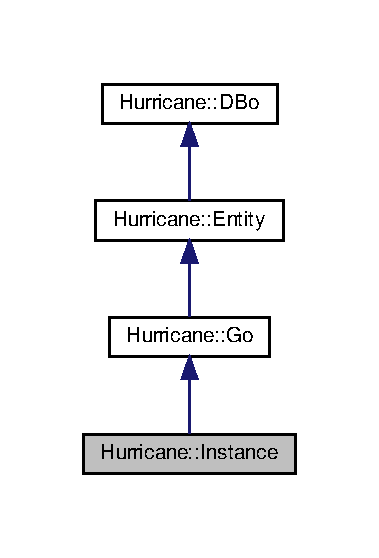
\includegraphics[width=182pt]{classHurricane_1_1Instance__inherit__graph}
\end{center}
\end{figure}
\doxysubsection*{Classes}
\begin{DoxyCompactItemize}
\item 
class \mbox{\hyperlink{classHurricane_1_1Instance_1_1PlacementStatus}{Placement\+Status}}
\begin{DoxyCompactList}\small\item\em \mbox{\hyperlink{classHurricane_1_1Instance}{Instance}} Placement Status ({\bfseries{API}}) \end{DoxyCompactList}\end{DoxyCompactItemize}
\doxysubsection*{Public Types}
\begin{DoxyCompactItemize}
\item 
typedef \mbox{\hyperlink{classHurricane_1_1Go}{Go}} \mbox{\hyperlink{classHurricane_1_1Instance_a227e1f98670e466328ca95fe45546590}{Inherit}}
\end{DoxyCompactItemize}
\doxysubsection*{Public Member Functions}
\begin{DoxyCompactItemize}
\item 
const \mbox{\hyperlink{classHurricane_1_1Name}{Name}} \& \mbox{\hyperlink{classHurricane_1_1Instance_aa48280b4d7127d283c89983cf7a42c23}{get\+Name}} () const
\item 
\mbox{\hyperlink{classHurricane_1_1Cell}{Cell}} $\ast$ \mbox{\hyperlink{classHurricane_1_1Instance_ad08a772e5e36582070cdc407cfcc1a64}{get\+Master\+Cell}} () const
\item 
const \mbox{\hyperlink{classHurricane_1_1Transformation}{Transformation}} \& \mbox{\hyperlink{classHurricane_1_1Instance_a5042051d648fd93548dc6c5e14782645}{get\+Transformation}} () const
\item 
\mbox{\hyperlink{classHurricane_1_1Plug}{Plug}} $\ast$ \mbox{\hyperlink{classHurricane_1_1Instance_a1afe07edc0374ddfb505b4973c902834}{get\+Plug}} (const \mbox{\hyperlink{classHurricane_1_1Net}{Net}} $\ast$master\+Net) const
\item 
\mbox{\hyperlink{namespaceHurricane_ac8335d2057483ee7a935c15a9460c64f}{Plugs}} \mbox{\hyperlink{classHurricane_1_1Instance_a5433b64eed99f9a099004490fae6d8f4}{get\+Plugs}} () const
\item 
\mbox{\hyperlink{namespaceHurricane_ac8335d2057483ee7a935c15a9460c64f}{Plugs}} \mbox{\hyperlink{classHurricane_1_1Instance_a18beeab0def83c20e25a710b30dd8ca9}{get\+Connected\+Plugs}} () const
\item 
\mbox{\hyperlink{namespaceHurricane_ac8335d2057483ee7a935c15a9460c64f}{Plugs}} \mbox{\hyperlink{classHurricane_1_1Instance_a9622b8b961f459469c275b3dafe1733c}{get\+Unconnected\+Plugs}} () const
\item 
\mbox{\hyperlink{classHurricane_1_1Path}{Path}} \mbox{\hyperlink{classHurricane_1_1Instance_a4d13f5b9294d0361b724b5824fd86378}{get\+Path}} (const \mbox{\hyperlink{classHurricane_1_1Path}{Path}} \&tail\+Path=\mbox{\hyperlink{classHurricane_1_1Path}{Path}}()) const
\item 
\mbox{\hyperlink{classHurricane_1_1Box}{Box}} \mbox{\hyperlink{classHurricane_1_1Instance_a29bedbd05939bf43757ef036bb506d01}{get\+Abutment\+Box}} () const
\item 
void \mbox{\hyperlink{classHurricane_1_1Instance_ae3b67792d1659f1a20c6533b8843b905}{set\+Name}} (const \mbox{\hyperlink{classHurricane_1_1Name}{Name}} \&name)
\item 
void \mbox{\hyperlink{classHurricane_1_1Instance_a8890d2e1b2ba2542997454297e63512f}{set\+Transformation}} (const \mbox{\hyperlink{classHurricane_1_1Transformation}{Transformation}} \&transformation)
\item 
void \mbox{\hyperlink{classHurricane_1_1Instance_a9f626fd058c21ffc2ed5bfee8d29a853}{set\+Master\+Cell}} (\mbox{\hyperlink{classHurricane_1_1Cell}{Cell}} $\ast$master\+Cell, bool secure\+Flag=true)
\item 
void \mbox{\hyperlink{classHurricane_1_1Instance_adf28fcd01f6ff89c5435e83482f66d4c}{uniquify}} ()
\item 
\mbox{\hyperlink{classHurricane_1_1Instance}{Instance}} $\ast$ \mbox{\hyperlink{classHurricane_1_1Instance_ac5e111eef5767762e00f21fcd7a35702}{get\+Clone}} (\mbox{\hyperlink{classHurricane_1_1Cell}{Cell}} $\ast$clone\+Cell) const
\end{DoxyCompactItemize}
\doxysubsection*{Static Public Member Functions}
\begin{DoxyCompactItemize}
\item 
static \mbox{\hyperlink{classHurricane_1_1Instance}{Instance}} $\ast$ \mbox{\hyperlink{classHurricane_1_1Instance_ae130b66536e4536ba8852fb79abfb89e}{create}} (\mbox{\hyperlink{classHurricane_1_1Cell}{Cell}} $\ast$cell, const \mbox{\hyperlink{classHurricane_1_1Name}{Name}} \&name, \mbox{\hyperlink{classHurricane_1_1Cell}{Cell}} $\ast$master\+Cell, bool secure\+Flag=true)
\item 
static \mbox{\hyperlink{classHurricane_1_1Instance}{Instance}} $\ast$ \mbox{\hyperlink{classHurricane_1_1Instance_ad5784305151e45c9d949a74bd85aaa36}{create}} (\mbox{\hyperlink{classHurricane_1_1Cell}{Cell}} $\ast$cell, const \mbox{\hyperlink{classHurricane_1_1Name}{Name}} \&name, \mbox{\hyperlink{classHurricane_1_1Cell}{Cell}} $\ast$master\+Cell, const \mbox{\hyperlink{classHurricane_1_1Transformation}{Transformation}} \&transformation, const \mbox{\hyperlink{classHurricane_1_1Instance_1_1PlacementStatus}{Placement\+Status}} \&placementstatus, bool secure\+Flag=true)
\item 
static \mbox{\hyperlink{namespaceHurricane_a889ec1441e1876d9addf89dfab32e772}{Instance\+Filter}} \mbox{\hyperlink{classHurricane_1_1Instance_ae2bc936dfecfaf70a0052959b4b2861e}{get\+Is\+Under\+Filter}} (const \mbox{\hyperlink{classHurricane_1_1Box}{Box}} \&area)
\end{DoxyCompactItemize}


\doxysubsection{Detailed Description}
\mbox{\hyperlink{classHurricane_1_1Instance}{Instance}} description ({\bfseries{API}}) 

\hypertarget{classHurricane_1_1Instance_secInstanceIntro}{}\doxysubsection{Introduction}\label{classHurricane_1_1Instance_secInstanceIntro}
Instances provide the capability to build hierarchical assemblies. An instance belongs to a cell (the \char`\"{}$<$b$>$owner                cell$<$/b$>$\char`\"{}) and references (calls) a model cell which we will call the \char`\"{}$<$b$>$mater cell$<$/b$>$\char`\"{}. Seen from the other hand, a cell may be the master cell of many instances belonging to other cells, this set of instances is named the \char`\"{}$<$b$>$slave                instances$<$/b$>$\char`\"{} of this cell (it is empty for the top most cell of a hierachical assembly, as well as for all cells from the library which are not instanciated in the current design).\hypertarget{classHurricane_1_1Instance_secInstancePlacement}{}\doxysubsection{Placement Status}\label{classHurricane_1_1Instance_secInstancePlacement}
See \mbox{\hyperlink{classHurricane_1_1Instance_1_1PlacementStatus}{Instance\+::\+Placement\+Status}} and \mbox{\hyperlink{classHurricane_1_1Instance_1_1PlacementStatus_af76cc0838783b3eb3a515eb3c3e0f7bf}{Instance\+::\+Placement\+Status\+::\+Code}}.

An \mbox{\hyperlink{classHurricane_1_1Instance}{Instance}} can have three kind of placement status\+:
\begin{DoxyItemize}
\item \mbox{\hyperlink{classHurricane_1_1Instance_1_1PlacementStatus_af76cc0838783b3eb3a515eb3c3e0f7bfa3e19a0a1b3e8c8fd860164df7f935216}{Instance\+::\+Placement\+Status\+::\+UNPLACED}} \+: the instance doesn\textquotesingle{}t have a meaningful position. It shouldn\textquotesingle{}t be materialized either. It\textquotesingle{}s position therfore shouldn\textquotesingle{}t be used.
\item \mbox{\hyperlink{classHurricane_1_1Instance_1_1PlacementStatus_af76cc0838783b3eb3a515eb3c3e0f7bfaf3589c11ecd7d5de63db24826b74d457}{Instance\+::\+Placement\+Status\+::\+PLACED}} \+: the instance has be placed manually or by an automated tool. It is movable.
\item \mbox{\hyperlink{classHurricane_1_1Instance_1_1PlacementStatus_af76cc0838783b3eb3a515eb3c3e0f7bfa47be8a40f04081635fe24485ae7c6bd7}{Instance\+::\+Placement\+Status\+::\+FIXED}} \+: the instance is placed and mustn\textquotesingle{}t be moved by automated tools. It can still be moved manually.
\end{DoxyItemize}\hypertarget{classHurricane_1_1Instance_secInstancePredefinedFilters}{}\doxysubsection{Predefined filters}\label{classHurricane_1_1Instance_secInstancePredefinedFilters}
{\bfseries{\mbox{\hyperlink{classHurricane_1_1Instance_ae2bc936dfecfaf70a0052959b4b2861e}{Hurricane\+::\+Instance\+::get\+Is\+Under\+Filter}}}}\hypertarget{classHurricane_1_1Instance_secInstanceDestroy}{}\doxysubsection{Instance Destruction}\label{classHurricane_1_1Instance_secInstanceDestroy}
When the \mbox{\hyperlink{classHurricane_1_1DBo_a67febf5bf9c8b322674648688639728b}{Instance\+::destroy()}} method is called, if the master \mbox{\hyperlink{classHurricane_1_1Cell}{Cell}} is uniquified, that is, is unique {\bfseries{and}} a copy of the reference \mbox{\hyperlink{classHurricane_1_1Cell}{Cell}}, it is destroyed as well. That state means that the master \mbox{\hyperlink{classHurricane_1_1Cell}{Cell}} has been created for the only purpose as to serve as a model for this peculiar \mbox{\hyperlink{classHurricane_1_1Instance}{Instance}}. It is then logical that it should be removed with it. 

\doxysubsection{Member Typedef Documentation}
\mbox{\Hypertarget{classHurricane_1_1Instance_a227e1f98670e466328ca95fe45546590}\label{classHurricane_1_1Instance_a227e1f98670e466328ca95fe45546590}} 
\index{Hurricane::Instance@{Hurricane::Instance}!Inherit@{Inherit}}
\index{Inherit@{Inherit}!Hurricane::Instance@{Hurricane::Instance}}
\doxysubsubsection{\texorpdfstring{Inherit}{Inherit}}
{\footnotesize\ttfamily \mbox{\hyperlink{classHurricane_1_1Instance_a227e1f98670e466328ca95fe45546590}{Hurricane\+::\+Instance\+::\+Inherit}}}

Useful for calling upon methods of the base class without knowing it. 

\doxysubsection{Member Function Documentation}
\mbox{\Hypertarget{classHurricane_1_1Instance_ae130b66536e4536ba8852fb79abfb89e}\label{classHurricane_1_1Instance_ae130b66536e4536ba8852fb79abfb89e}} 
\index{Hurricane::Instance@{Hurricane::Instance}!create@{create}}
\index{create@{create}!Hurricane::Instance@{Hurricane::Instance}}
\doxysubsubsection{\texorpdfstring{create()}{create()}\hspace{0.1cm}{\footnotesize\ttfamily [1/2]}}
{\footnotesize\ttfamily \mbox{\hyperlink{classHurricane_1_1Instance}{Instance}} $\ast$ Hurricane\+::\+Instance\+::create (\begin{DoxyParamCaption}\item[{\mbox{\hyperlink{classHurricane_1_1Cell}{Cell}} $\ast$}]{cell,  }\item[{const \mbox{\hyperlink{classHurricane_1_1Name}{Name}} \&}]{name,  }\item[{\mbox{\hyperlink{classHurricane_1_1Cell}{Cell}} $\ast$}]{master\+Cell,  }\item[{bool}]{secure\+Flag = {\ttfamily true} }\end{DoxyParamCaption})\hspace{0.3cm}{\ttfamily [static]}}

No description. \mbox{\Hypertarget{classHurricane_1_1Instance_ad5784305151e45c9d949a74bd85aaa36}\label{classHurricane_1_1Instance_ad5784305151e45c9d949a74bd85aaa36}} 
\index{Hurricane::Instance@{Hurricane::Instance}!create@{create}}
\index{create@{create}!Hurricane::Instance@{Hurricane::Instance}}
\doxysubsubsection{\texorpdfstring{create()}{create()}\hspace{0.1cm}{\footnotesize\ttfamily [2/2]}}
{\footnotesize\ttfamily \mbox{\hyperlink{classHurricane_1_1Instance}{Instance}} $\ast$ Hurricane\+::\+Instance\+::create (\begin{DoxyParamCaption}\item[{\mbox{\hyperlink{classHurricane_1_1Cell}{Cell}} $\ast$}]{cell,  }\item[{const \mbox{\hyperlink{classHurricane_1_1Name}{Name}} \&}]{name,  }\item[{\mbox{\hyperlink{classHurricane_1_1Cell}{Cell}} $\ast$}]{master\+Cell,  }\item[{const \mbox{\hyperlink{classHurricane_1_1Transformation}{Transformation}} \&}]{transformation,  }\item[{const \mbox{\hyperlink{classHurricane_1_1Instance_1_1PlacementStatus}{Placement\+Status}} \&}]{placementstatus,  }\item[{bool}]{secure\+Flag = {\ttfamily true} }\end{DoxyParamCaption})\hspace{0.3cm}{\ttfamily [static]}}

Create and return a pointer to a new instance of name {\ttfamily $<$name$>$} belonging to the cell {\ttfamily $<$cell$>$} and refering the cell {\ttfamily $<$master\+Cell$>$} through a transformation {\ttfamily $<$transformation$>$} if it is provided (else the identity transform is assumed).

\begin{DoxyParagraph}{Caution\+: Throws an exception if the cell {\ttfamily $<$cell$>$} is null, if the }
{\ttfamily $<$master\+Cell$>$} is null, if an instance of same name already exists or if a cyclic assembly is detected.
\end{DoxyParagraph}
\begin{DoxyRemark}{Remarks}
If the {\ttfamily $<$secure\+Flag$>$} is set to {\bfseries{false}} the verification of the lack of cyclic assembly is skipped (you save some cpu time, but at your own risks). 
\end{DoxyRemark}
\mbox{\Hypertarget{classHurricane_1_1Instance_aa48280b4d7127d283c89983cf7a42c23}\label{classHurricane_1_1Instance_aa48280b4d7127d283c89983cf7a42c23}} 
\index{Hurricane::Instance@{Hurricane::Instance}!getName@{getName}}
\index{getName@{getName}!Hurricane::Instance@{Hurricane::Instance}}
\doxysubsubsection{\texorpdfstring{getName()}{getName()}}
{\footnotesize\ttfamily const \mbox{\hyperlink{classHurricane_1_1Name}{Name}} \& Hurricane\+::\+Instance\+::get\+Name (\begin{DoxyParamCaption}{ }\end{DoxyParamCaption}) const\hspace{0.3cm}{\ttfamily [inline]}}

{\bfseries{Returns\+:}} the instance name. \mbox{\Hypertarget{classHurricane_1_1Instance_ad08a772e5e36582070cdc407cfcc1a64}\label{classHurricane_1_1Instance_ad08a772e5e36582070cdc407cfcc1a64}} 
\index{Hurricane::Instance@{Hurricane::Instance}!getMasterCell@{getMasterCell}}
\index{getMasterCell@{getMasterCell}!Hurricane::Instance@{Hurricane::Instance}}
\doxysubsubsection{\texorpdfstring{getMasterCell()}{getMasterCell()}}
{\footnotesize\ttfamily \mbox{\hyperlink{classHurricane_1_1Cell}{Cell}} $\ast$ Hurricane\+::\+Instance\+::get\+Master\+Cell (\begin{DoxyParamCaption}{ }\end{DoxyParamCaption}) const\hspace{0.3cm}{\ttfamily [inline]}}

{\bfseries{Returns\+:}} the cell model referenced by the instance. \mbox{\Hypertarget{classHurricane_1_1Instance_a5042051d648fd93548dc6c5e14782645}\label{classHurricane_1_1Instance_a5042051d648fd93548dc6c5e14782645}} 
\index{Hurricane::Instance@{Hurricane::Instance}!getTransformation@{getTransformation}}
\index{getTransformation@{getTransformation}!Hurricane::Instance@{Hurricane::Instance}}
\doxysubsubsection{\texorpdfstring{getTransformation()}{getTransformation()}}
{\footnotesize\ttfamily const \mbox{\hyperlink{classHurricane_1_1Transformation}{Transformation}} \& Hurricane\+::\+Instance\+::get\+Transformation (\begin{DoxyParamCaption}{ }\end{DoxyParamCaption}) const\hspace{0.3cm}{\ttfamily [inline]}}

{\bfseries{Returns\+:}} the transformation associated to the instance. \mbox{\Hypertarget{classHurricane_1_1Instance_a1afe07edc0374ddfb505b4973c902834}\label{classHurricane_1_1Instance_a1afe07edc0374ddfb505b4973c902834}} 
\index{Hurricane::Instance@{Hurricane::Instance}!getPlug@{getPlug}}
\index{getPlug@{getPlug}!Hurricane::Instance@{Hurricane::Instance}}
\doxysubsubsection{\texorpdfstring{getPlug()}{getPlug()}}
{\footnotesize\ttfamily \mbox{\hyperlink{classHurricane_1_1Plug}{Plug}} $\ast$ Hurricane\+::\+Instance\+::get\+Plug (\begin{DoxyParamCaption}\item[{const \mbox{\hyperlink{classHurricane_1_1Net}{Net}} $\ast$}]{master\+Net }\end{DoxyParamCaption}) const\hspace{0.3cm}{\ttfamily [inline]}}

{\bfseries{Returns\+:}} the plug associated to the {\ttfamily $<$master\+Net$>$} if it exists or else NULL (if the net is not external). \mbox{\Hypertarget{classHurricane_1_1Instance_a5433b64eed99f9a099004490fae6d8f4}\label{classHurricane_1_1Instance_a5433b64eed99f9a099004490fae6d8f4}} 
\index{Hurricane::Instance@{Hurricane::Instance}!getPlugs@{getPlugs}}
\index{getPlugs@{getPlugs}!Hurricane::Instance@{Hurricane::Instance}}
\doxysubsubsection{\texorpdfstring{getPlugs()}{getPlugs()}}
{\footnotesize\ttfamily \mbox{\hyperlink{namespaceHurricane_ac8335d2057483ee7a935c15a9460c64f}{Plugs}} Hurricane\+::\+Instance\+::get\+Plugs (\begin{DoxyParamCaption}{ }\end{DoxyParamCaption}) const\hspace{0.3cm}{\ttfamily [inline]}}

{\bfseries{Returns\+:}} the collection of instance plugs.

\begin{DoxyParagraph}{Important\+:\textbackslash{}n Each external net of the master cell of the instance has by }
construction an associated plug. This one may be connected or not to a net in the owner cell of the instance. 
\end{DoxyParagraph}
\mbox{\Hypertarget{classHurricane_1_1Instance_a18beeab0def83c20e25a710b30dd8ca9}\label{classHurricane_1_1Instance_a18beeab0def83c20e25a710b30dd8ca9}} 
\index{Hurricane::Instance@{Hurricane::Instance}!getConnectedPlugs@{getConnectedPlugs}}
\index{getConnectedPlugs@{getConnectedPlugs}!Hurricane::Instance@{Hurricane::Instance}}
\doxysubsubsection{\texorpdfstring{getConnectedPlugs()}{getConnectedPlugs()}}
{\footnotesize\ttfamily \mbox{\hyperlink{namespaceHurricane_ac8335d2057483ee7a935c15a9460c64f}{Plugs}} Hurricane\+::\+Instance\+::get\+Connected\+Plugs (\begin{DoxyParamCaption}{ }\end{DoxyParamCaption}) const}

{\bfseries{Returns\+:}} the collection of instance plugs which are effectively connected. \mbox{\Hypertarget{classHurricane_1_1Instance_a9622b8b961f459469c275b3dafe1733c}\label{classHurricane_1_1Instance_a9622b8b961f459469c275b3dafe1733c}} 
\index{Hurricane::Instance@{Hurricane::Instance}!getUnconnectedPlugs@{getUnconnectedPlugs}}
\index{getUnconnectedPlugs@{getUnconnectedPlugs}!Hurricane::Instance@{Hurricane::Instance}}
\doxysubsubsection{\texorpdfstring{getUnconnectedPlugs()}{getUnconnectedPlugs()}}
{\footnotesize\ttfamily \mbox{\hyperlink{namespaceHurricane_ac8335d2057483ee7a935c15a9460c64f}{Plugs}} Hurricane\+::\+Instance\+::get\+Unconnected\+Plugs (\begin{DoxyParamCaption}{ }\end{DoxyParamCaption}) const}

{\bfseries{Returns\+:}} the collection of instance plugs which are not connected. \mbox{\Hypertarget{classHurricane_1_1Instance_a4d13f5b9294d0361b724b5824fd86378}\label{classHurricane_1_1Instance_a4d13f5b9294d0361b724b5824fd86378}} 
\index{Hurricane::Instance@{Hurricane::Instance}!getPath@{getPath}}
\index{getPath@{getPath}!Hurricane::Instance@{Hurricane::Instance}}
\doxysubsubsection{\texorpdfstring{getPath()}{getPath()}}
{\footnotesize\ttfamily \mbox{\hyperlink{classHurricane_1_1Path}{Path}} Hurricane\+::\+Instance\+::get\+Path (\begin{DoxyParamCaption}\item[{const \mbox{\hyperlink{classHurricane_1_1Path}{Path}} \&}]{tail\+Path = {\ttfamily \mbox{\hyperlink{classHurricane_1_1Path}{Path}}()} }\end{DoxyParamCaption}) const}

{\bfseries{Returns\+:}} the path composed of the instance solely.

{\bfseries{Returns\+:}} the path resulting of the concatenation of the instance and the tail path (possibly empty).

\begin{DoxyParagraph}{Caution\+: An exception will be thrown if the tail path is not }
consistent with the instance (that is if the owner cell of the tail path is not the master cell of the instance). 
\end{DoxyParagraph}
\mbox{\Hypertarget{classHurricane_1_1Instance_a29bedbd05939bf43757ef036bb506d01}\label{classHurricane_1_1Instance_a29bedbd05939bf43757ef036bb506d01}} 
\index{Hurricane::Instance@{Hurricane::Instance}!getAbutmentBox@{getAbutmentBox}}
\index{getAbutmentBox@{getAbutmentBox}!Hurricane::Instance@{Hurricane::Instance}}
\doxysubsubsection{\texorpdfstring{getAbutmentBox()}{getAbutmentBox()}}
{\footnotesize\ttfamily \mbox{\hyperlink{classHurricane_1_1Box}{Box}} Hurricane\+::\+Instance\+::get\+Abutment\+Box (\begin{DoxyParamCaption}{ }\end{DoxyParamCaption}) const}

{\bfseries{Returns\+:}} the abutment box of the instance, that is the abutment box of the master cell to which has been applied the instance transformation. \mbox{\Hypertarget{classHurricane_1_1Instance_ae2bc936dfecfaf70a0052959b4b2861e}\label{classHurricane_1_1Instance_ae2bc936dfecfaf70a0052959b4b2861e}} 
\index{Hurricane::Instance@{Hurricane::Instance}!getIsUnderFilter@{getIsUnderFilter}}
\index{getIsUnderFilter@{getIsUnderFilter}!Hurricane::Instance@{Hurricane::Instance}}
\doxysubsubsection{\texorpdfstring{getIsUnderFilter()}{getIsUnderFilter()}}
{\footnotesize\ttfamily \mbox{\hyperlink{namespaceHurricane_a889ec1441e1876d9addf89dfab32e772}{Instance\+Filter}} Hurricane\+::\+Instance\+::get\+Is\+Under\+Filter (\begin{DoxyParamCaption}\item[{const \mbox{\hyperlink{classHurricane_1_1Box}{Box}} \&}]{area }\end{DoxyParamCaption})\hspace{0.3cm}{\ttfamily [static]}}

{\bfseries{Returns\+:}} the filter selecting instances which intersect the given area. \mbox{\Hypertarget{classHurricane_1_1Instance_ae3b67792d1659f1a20c6533b8843b905}\label{classHurricane_1_1Instance_ae3b67792d1659f1a20c6533b8843b905}} 
\index{Hurricane::Instance@{Hurricane::Instance}!setName@{setName}}
\index{setName@{setName}!Hurricane::Instance@{Hurricane::Instance}}
\doxysubsubsection{\texorpdfstring{setName()}{setName()}}
{\footnotesize\ttfamily void Hurricane\+::\+Instance\+::set\+Name (\begin{DoxyParamCaption}\item[{const \mbox{\hyperlink{classHurricane_1_1Name}{Name}} \&}]{name }\end{DoxyParamCaption})}

Allows to change the instance name.

\begin{DoxyRemark}{Remarks}
Throws an exception if the name is empty or if an instance with the same name exists in the owner cell. 
\end{DoxyRemark}
\mbox{\Hypertarget{classHurricane_1_1Instance_a8890d2e1b2ba2542997454297e63512f}\label{classHurricane_1_1Instance_a8890d2e1b2ba2542997454297e63512f}} 
\index{Hurricane::Instance@{Hurricane::Instance}!setTransformation@{setTransformation}}
\index{setTransformation@{setTransformation}!Hurricane::Instance@{Hurricane::Instance}}
\doxysubsubsection{\texorpdfstring{setTransformation()}{setTransformation()}}
{\footnotesize\ttfamily void Hurricane\+::\+Instance\+::set\+Transformation (\begin{DoxyParamCaption}\item[{const \mbox{\hyperlink{classHurricane_1_1Transformation}{Transformation}} \&}]{transformation }\end{DoxyParamCaption})}

Allows to modify the instance transformation. \mbox{\Hypertarget{classHurricane_1_1Instance_a9f626fd058c21ffc2ed5bfee8d29a853}\label{classHurricane_1_1Instance_a9f626fd058c21ffc2ed5bfee8d29a853}} 
\index{Hurricane::Instance@{Hurricane::Instance}!setMasterCell@{setMasterCell}}
\index{setMasterCell@{setMasterCell}!Hurricane::Instance@{Hurricane::Instance}}
\doxysubsubsection{\texorpdfstring{setMasterCell()}{setMasterCell()}}
{\footnotesize\ttfamily void Hurricane\+::\+Instance\+::set\+Master\+Cell (\begin{DoxyParamCaption}\item[{\mbox{\hyperlink{classHurricane_1_1Cell}{Cell}} $\ast$}]{master\+Cell,  }\item[{bool}]{secure\+Flag = {\ttfamily true} }\end{DoxyParamCaption})}

Allows to change the cell referenced by this instance.

\begin{DoxyParagraph}{Caution\+: Throws an exception if either the cell is null, a cyclic }
assembly is detected or the substitution can\textquotesingle{}t succeed.
\end{DoxyParagraph}
\begin{DoxyRemark}{Remarks}
If the {\ttfamily $<$secure\+Flag$>$} is set to {\bfseries{false}} the verification of the lack of cyclic assembly is skipped (you save some cpu time, but at your own risks).
\end{DoxyRemark}
\begin{DoxyParagraph}{Important\+:\textbackslash{}n In order to succeed with the substitution, it is necessary }
that for each connected plug, refering an external net of the old master cell, a net of same name can be found in the new master cell.
\end{DoxyParagraph}
The properties of the instance, of its existing plugs and of the different occurences of those ones are preserved. On the other hand, all the hierarchical pathes going through that instance and not ending on it, as well as all associated occurences, become obsolete. The properties attached to those occurences are therefore deleted. \mbox{\Hypertarget{classHurricane_1_1Instance_adf28fcd01f6ff89c5435e83482f66d4c}\label{classHurricane_1_1Instance_adf28fcd01f6ff89c5435e83482f66d4c}} 
\index{Hurricane::Instance@{Hurricane::Instance}!uniquify@{uniquify}}
\index{uniquify@{uniquify}!Hurricane::Instance@{Hurricane::Instance}}
\doxysubsubsection{\texorpdfstring{uniquify()}{uniquify()}}
{\footnotesize\ttfamily void Hurricane\+::\+Instance\+::uniquify (\begin{DoxyParamCaption}{ }\end{DoxyParamCaption})}

Replace the {\ttfamily } $<$master\+Cell$>$ of this instance by a cloned copy.

\begin{DoxySeeAlso}{See also}
\mbox{\hyperlink{classHurricane_1_1Cell_a092f53c7f517ecc70d9ba375296c5d5b}{Cell\+::get\+Clone()}}. 
\end{DoxySeeAlso}
\mbox{\Hypertarget{classHurricane_1_1Instance_ac5e111eef5767762e00f21fcd7a35702}\label{classHurricane_1_1Instance_ac5e111eef5767762e00f21fcd7a35702}} 
\index{Hurricane::Instance@{Hurricane::Instance}!getClone@{getClone}}
\index{getClone@{getClone}!Hurricane::Instance@{Hurricane::Instance}}
\doxysubsubsection{\texorpdfstring{getClone()}{getClone()}}
{\footnotesize\ttfamily \mbox{\hyperlink{classHurricane_1_1Instance}{Instance}} $\ast$ Hurricane\+::\+Instance\+::get\+Clone (\begin{DoxyParamCaption}\item[{\mbox{\hyperlink{classHurricane_1_1Cell}{Cell}} $\ast$}]{clone\+Cell }\end{DoxyParamCaption}) const}

Build a duplicate of instance ({\ttfamily } $<$this$>$) inside a cloned \mbox{\hyperlink{classHurricane_1_1Cell}{Cell}} {\ttfamily } $<$clone\+Cell$>$. The connections (\mbox{\hyperlink{classHurricane_1_1Plug}{Plug}}) on the copied instance are copied. That is, connected to \mbox{\hyperlink{classHurricane_1_1Net}{Net}} with identical names in {\ttfamily } $<$clone\+Cell$>$.

\begin{DoxyParagraph}{Important\+:\textbackslash{}n In {\ttfamily }, a copy (by name) of all the nets this instance}
is connected to must exits. 
\end{DoxyParagraph}


The documentation for this class was generated from the following files\+:\begin{DoxyCompactItemize}
\item 
Instance.\+h\item 
Instance.\+dox\end{DoxyCompactItemize}

\hypertarget{classHurricane_1_1Interruption}{}\doxysection{Hurricane\+::Interruption Class Reference}
\label{classHurricane_1_1Interruption}\index{Hurricane::Interruption@{Hurricane::Interruption}}


\mbox{\hyperlink{classHurricane_1_1Interruption}{Interruption}} description ({\bfseries{API}})  




Inheritance diagram for Hurricane\+::Interruption\+:\nopagebreak
\begin{figure}[H]
\begin{center}
\leavevmode
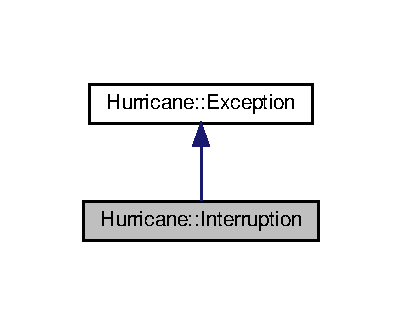
\includegraphics[width=193pt]{classHurricane_1_1Interruption__inherit__graph}
\end{center}
\end{figure}
\doxysubsection*{Public Types}
\begin{DoxyCompactItemize}
\item 
typedef \mbox{\hyperlink{classHurricane_1_1Exception}{Exception}} \mbox{\hyperlink{classHurricane_1_1Interruption_a47ecad9b4b2bd34a21de4a0d6fdf1f5d}{Inherit}}
\end{DoxyCompactItemize}
\doxysubsection*{Public Member Functions}
\begin{DoxyCompactItemize}
\item 
\mbox{\hyperlink{classHurricane_1_1Interruption_ae6375068418b2898b95c3cb7974e051c}{Interruption}} (const string \&reason, int code=0)
\item 
\mbox{\hyperlink{classHurricane_1_1Interruption_ad84fb4212bce9f3a85b90b4a969226a6}{Interruption}} (const \mbox{\hyperlink{classHurricane_1_1Interruption}{Interruption}} \&interruption)
\item 
\mbox{\hyperlink{classHurricane_1_1Interruption}{Interruption}} \& \mbox{\hyperlink{classHurricane_1_1Interruption_a3c528402a234e354e508b5b7512475bc}{operator=}} (const \mbox{\hyperlink{classHurricane_1_1Interruption}{Interruption}} \&interruption)
\end{DoxyCompactItemize}
\doxysubsection*{Additional Inherited Members}


\doxysubsection{Detailed Description}
\mbox{\hyperlink{classHurricane_1_1Interruption}{Interruption}} description ({\bfseries{API}}) 

\hypertarget{classHurricane_1_1Interruption_secInterruptionIntro}{}\doxysubsection{Introduction}\label{classHurricane_1_1Interruption_secInterruptionIntro}
Interruptions are neither errors nor warnings. They are used to suspend a potentially lengthy action (like a display refresh). We could have used errors or warning but it is wiser to use a specific type. 

\doxysubsection{Member Typedef Documentation}
\mbox{\Hypertarget{classHurricane_1_1Interruption_a47ecad9b4b2bd34a21de4a0d6fdf1f5d}\label{classHurricane_1_1Interruption_a47ecad9b4b2bd34a21de4a0d6fdf1f5d}} 
\index{Hurricane::Interruption@{Hurricane::Interruption}!Inherit@{Inherit}}
\index{Inherit@{Inherit}!Hurricane::Interruption@{Hurricane::Interruption}}
\doxysubsubsection{\texorpdfstring{Inherit}{Inherit}}
{\footnotesize\ttfamily \mbox{\hyperlink{classHurricane_1_1Interruption_a47ecad9b4b2bd34a21de4a0d6fdf1f5d}{Hurricane\+::\+Interruption\+::\+Inherit}}}

Useful for calling the base class methods without knowing this class. 

\doxysubsection{Constructor \& Destructor Documentation}
\mbox{\Hypertarget{classHurricane_1_1Interruption_ae6375068418b2898b95c3cb7974e051c}\label{classHurricane_1_1Interruption_ae6375068418b2898b95c3cb7974e051c}} 
\index{Hurricane::Interruption@{Hurricane::Interruption}!Interruption@{Interruption}}
\index{Interruption@{Interruption}!Hurricane::Interruption@{Hurricane::Interruption}}
\doxysubsubsection{\texorpdfstring{Interruption()}{Interruption()}\hspace{0.1cm}{\footnotesize\ttfamily [1/2]}}
{\footnotesize\ttfamily Hurricane\+::\+Interruption\+::\+Interruption (\begin{DoxyParamCaption}\item[{const string \&}]{reason,  }\item[{int}]{code = {\ttfamily 0} }\end{DoxyParamCaption})}

Builds an interruption characterized by a reason and a code useful within a switch. \mbox{\Hypertarget{classHurricane_1_1Interruption_ad84fb4212bce9f3a85b90b4a969226a6}\label{classHurricane_1_1Interruption_ad84fb4212bce9f3a85b90b4a969226a6}} 
\index{Hurricane::Interruption@{Hurricane::Interruption}!Interruption@{Interruption}}
\index{Interruption@{Interruption}!Hurricane::Interruption@{Hurricane::Interruption}}
\doxysubsubsection{\texorpdfstring{Interruption()}{Interruption()}\hspace{0.1cm}{\footnotesize\ttfamily [2/2]}}
{\footnotesize\ttfamily Hurricane\+::\+Interruption\+::\+Interruption (\begin{DoxyParamCaption}\item[{const \mbox{\hyperlink{classHurricane_1_1Interruption}{Interruption}} \&}]{interruption }\end{DoxyParamCaption})}

Copy constructor. 

\doxysubsection{Member Function Documentation}
\mbox{\Hypertarget{classHurricane_1_1Interruption_a3c528402a234e354e508b5b7512475bc}\label{classHurricane_1_1Interruption_a3c528402a234e354e508b5b7512475bc}} 
\index{Hurricane::Interruption@{Hurricane::Interruption}!operator=@{operator=}}
\index{operator=@{operator=}!Hurricane::Interruption@{Hurricane::Interruption}}
\doxysubsubsection{\texorpdfstring{operator=()}{operator=()}}
{\footnotesize\ttfamily \mbox{\hyperlink{classHurricane_1_1Interruption}{Interruption}} \& Hurricane\+::\+Interruption\+::operator= (\begin{DoxyParamCaption}\item[{const \mbox{\hyperlink{classHurricane_1_1Interruption}{Interruption}} \&}]{interruption }\end{DoxyParamCaption})}

Assignment operator. 

The documentation for this class was generated from the following files\+:\begin{DoxyCompactItemize}
\item 
Interruption.\+h\item 
Interruption.\+dox\end{DoxyCompactItemize}

\hypertarget{classHurricane_1_1Interval}{}\doxysection{Hurricane\+::Interval Class Reference}
\label{classHurricane_1_1Interval}\index{Hurricane::Interval@{Hurricane::Interval}}


\mbox{\hyperlink{classHurricane_1_1Interval}{Interval}} description ({\bfseries{API}})  


\doxysubsection*{Public Member Functions}
\begin{DoxyCompactItemize}
\item 
\mbox{\hyperlink{classHurricane_1_1Interval_a02b04ad7ca380422098992fa8ff5f546}{Interval}} (bool \mbox{\hyperlink{classHurricane_1_1Interval_a1e171021dcd5c0dc7e8afb0b2324c5ee}{make\+Empty}}=true)
\item 
\mbox{\hyperlink{classHurricane_1_1Interval_ace4173705b4dbcf6c00cd83bb61c4d43}{Interval}} (const \mbox{\hyperlink{classHurricane_1_1DbU_a4fbfa3e8c89347af76c9628ea06c4146}{Db\+U\+::\+Unit}} \&)
\item 
\mbox{\hyperlink{classHurricane_1_1Interval_a35e2ddc881a5b0c3ff8003d52f6298bb}{Interval}} (const \mbox{\hyperlink{classHurricane_1_1DbU_a4fbfa3e8c89347af76c9628ea06c4146}{Db\+U\+::\+Unit}} \&v1, const \mbox{\hyperlink{classHurricane_1_1DbU_a4fbfa3e8c89347af76c9628ea06c4146}{Db\+U\+::\+Unit}} \&v2)
\item 
\mbox{\hyperlink{classHurricane_1_1Interval_a2db3923eb057dd19f5320d93a09750d9}{Interval}} (const \mbox{\hyperlink{classHurricane_1_1Interval}{Interval}} \&)
\item 
\mbox{\hyperlink{classHurricane_1_1Interval}{Interval}} \& \mbox{\hyperlink{classHurricane_1_1Interval_a337b424cea8024f574726c3a2e4935b8}{operator=}} (const \mbox{\hyperlink{classHurricane_1_1Interval}{Interval}} \&)
\item 
bool \mbox{\hyperlink{classHurricane_1_1Interval_a1b022ac0ad975f168ac2b2689e6368c3}{operator==}} (const \mbox{\hyperlink{classHurricane_1_1Interval}{Interval}} \&) const
\item 
bool \mbox{\hyperlink{classHurricane_1_1Interval_a2e5a64c485269fb08fb762e1eb3bc374}{operator!=}} (const \mbox{\hyperlink{classHurricane_1_1Interval}{Interval}} \&) const
\item 
const \mbox{\hyperlink{classHurricane_1_1DbU_a4fbfa3e8c89347af76c9628ea06c4146}{Db\+U\+::\+Unit}} \& \mbox{\hyperlink{classHurricane_1_1Interval_a6e0deb1b38065375a78c7fd6885b5909}{get\+VMin}} () const
\item 
const \mbox{\hyperlink{classHurricane_1_1DbU_a4fbfa3e8c89347af76c9628ea06c4146}{Db\+U\+::\+Unit}} \& \mbox{\hyperlink{classHurricane_1_1Interval_a2f5ec659fde913492f89dc215001acb2}{get\+VMax}} () const
\item 
\mbox{\hyperlink{classHurricane_1_1DbU_a4fbfa3e8c89347af76c9628ea06c4146}{Db\+U\+::\+Unit}} \mbox{\hyperlink{classHurricane_1_1Interval_a6d12d0404054c7ccadab1afa6683a561}{get\+Center}} () const
\item 
\mbox{\hyperlink{classHurricane_1_1DbU_a4fbfa3e8c89347af76c9628ea06c4146}{Db\+U\+::\+Unit}} \mbox{\hyperlink{classHurricane_1_1Interval_a61d877fee3986f93c357910cd63f1caa}{get\+Size}} () const
\item 
\mbox{\hyperlink{classHurricane_1_1DbU_a4fbfa3e8c89347af76c9628ea06c4146}{Db\+U\+::\+Unit}} \mbox{\hyperlink{classHurricane_1_1Interval_abe66d75c0854ca0a76189801f0f7d0e3}{get\+Half\+Size}} () const
\item 
\mbox{\hyperlink{classHurricane_1_1Interval}{Interval}} \mbox{\hyperlink{classHurricane_1_1Interval_ac50b0e28faf03b54f81af109d942b569}{get\+Union}} (const \mbox{\hyperlink{classHurricane_1_1Interval}{Interval}} \&) const
\item 
\mbox{\hyperlink{classHurricane_1_1Interval}{Interval}} \mbox{\hyperlink{classHurricane_1_1Interval_a73130b484cf43ff3b48488780a926ead}{get\+Intersection}} (const \mbox{\hyperlink{classHurricane_1_1Interval}{Interval}} \&) const
\item 
bool \mbox{\hyperlink{classHurricane_1_1Interval_a5bf0292743d02f861a194c48c823c7ce}{is\+Empty}} () const
\item 
bool \mbox{\hyperlink{classHurricane_1_1Interval_acfc27bb7442f359db7d04c72fa8edeb8}{is\+Ponctual}} () const
\item 
bool \mbox{\hyperlink{classHurricane_1_1Interval_a84beba7ba34552e12e6cb9e462a94765}{contains}} (const \mbox{\hyperlink{classHurricane_1_1DbU_a4fbfa3e8c89347af76c9628ea06c4146}{Db\+U\+::\+Unit}} \&) const
\item 
bool \mbox{\hyperlink{classHurricane_1_1Interval_af613eb138f2035f50cba47057a074b2e}{contains}} (const \mbox{\hyperlink{classHurricane_1_1Interval}{Interval}} \&) const
\item 
bool \mbox{\hyperlink{classHurricane_1_1Interval_af4862b82fe5b37cdb3986a3b05245469}{intersect}} (const \mbox{\hyperlink{classHurricane_1_1Interval}{Interval}} \&, bool strict=false) const
\item 
\mbox{\hyperlink{classHurricane_1_1Interval}{Interval}} \& \mbox{\hyperlink{classHurricane_1_1Interval_a1e171021dcd5c0dc7e8afb0b2324c5ee}{make\+Empty}} ()
\item 
\mbox{\hyperlink{classHurricane_1_1Interval}{Interval}} \& \mbox{\hyperlink{classHurricane_1_1Interval_a142c3ec37ebe74c253b3fe0039ef2143}{inflate}} (const \mbox{\hyperlink{classHurricane_1_1DbU_a4fbfa3e8c89347af76c9628ea06c4146}{Db\+U\+::\+Unit}} \&dv)
\item 
\mbox{\hyperlink{classHurricane_1_1Interval}{Interval}} \& \mbox{\hyperlink{classHurricane_1_1Interval_ac311880a39d8e3db79bcbc5d3bb341a6}{inflate}} (const \mbox{\hyperlink{classHurricane_1_1DbU_a4fbfa3e8c89347af76c9628ea06c4146}{Db\+U\+::\+Unit}} \&dv\+Min, const \mbox{\hyperlink{classHurricane_1_1DbU_a4fbfa3e8c89347af76c9628ea06c4146}{Db\+U\+::\+Unit}} \&dv\+Max)
\item 
\mbox{\hyperlink{classHurricane_1_1Interval}{Interval}} \& \mbox{\hyperlink{classHurricane_1_1Interval_ab37a2b3ad247a0a5a4e4946d2b777bec}{merge}} (const \mbox{\hyperlink{classHurricane_1_1DbU_a4fbfa3e8c89347af76c9628ea06c4146}{Db\+U\+::\+Unit}} \&)
\item 
\mbox{\hyperlink{classHurricane_1_1Interval}{Interval}} \& \mbox{\hyperlink{classHurricane_1_1Interval_a99c17b60766c1146ad380ac9981008f7}{merge}} (const \mbox{\hyperlink{classHurricane_1_1Interval}{Interval}} \&)
\item 
\mbox{\hyperlink{classHurricane_1_1Interval}{Interval}} \& \mbox{\hyperlink{classHurricane_1_1Interval_a0eeaaa7eb5b4ade89719c57a2c284909}{intersection}} (const \mbox{\hyperlink{classHurricane_1_1DbU_a4fbfa3e8c89347af76c9628ea06c4146}{Db\+U\+::\+Unit}} \&v\+Min, const \mbox{\hyperlink{classHurricane_1_1DbU_a4fbfa3e8c89347af76c9628ea06c4146}{Db\+U\+::\+Unit}} \&v\+Max)
\item 
\mbox{\hyperlink{classHurricane_1_1Interval}{Interval}} \& \mbox{\hyperlink{classHurricane_1_1Interval_aea3de219c9e8316e19d71d44428b8dc4}{intersection}} (const \mbox{\hyperlink{classHurricane_1_1Interval}{Interval}} \&)
\item 
\mbox{\hyperlink{classHurricane_1_1Interval}{Interval}} \& \mbox{\hyperlink{classHurricane_1_1Interval_acf0aab51a74fe1216bfe112999066466}{translate}} (const \mbox{\hyperlink{classHurricane_1_1DbU_a4fbfa3e8c89347af76c9628ea06c4146}{Db\+U\+::\+Unit}} \&)
\end{DoxyCompactItemize}


\doxysubsection{Detailed Description}
\mbox{\hyperlink{classHurricane_1_1Interval}{Interval}} description ({\bfseries{API}}) 

\hypertarget{classHurricane_1_1Interval_secIntervalIntro}{}\doxysubsection{Introduction}\label{classHurricane_1_1Interval_secIntervalIntro}
Those objects represent intervals. They are defined by the values {\bfseries{VMin}} and {\bfseries{VMax}} which are representatives only when the interval is not empty. An interval is considered empty whenever it is not initialized or when it doesn\textquotesingle{}t represent a real interval like the intersection of two disjoint intervals.\hypertarget{classHurricane_1_1Interval_secIntervalRemark}{}\doxysubsection{Remark}\label{classHurricane_1_1Interval_secIntervalRemark}
All the function described in the chapter above return a reference on the modified interval, providing so the capability to apply to it a new modification. 

\doxysubsection{Constructor \& Destructor Documentation}
\mbox{\Hypertarget{classHurricane_1_1Interval_a02b04ad7ca380422098992fa8ff5f546}\label{classHurricane_1_1Interval_a02b04ad7ca380422098992fa8ff5f546}} 
\index{Hurricane::Interval@{Hurricane::Interval}!Interval@{Interval}}
\index{Interval@{Interval}!Hurricane::Interval@{Hurricane::Interval}}
\doxysubsubsection{\texorpdfstring{Interval()}{Interval()}\hspace{0.1cm}{\footnotesize\ttfamily [1/4]}}
{\footnotesize\ttfamily Hurricane\+::\+Interval\+::\+Interval (\begin{DoxyParamCaption}\item[{bool}]{make\+Empty = {\ttfamily true} }\end{DoxyParamCaption})}

Default constructor \+: the returned interval is empty if {\bfseries{make\+Empy}} is set to {\bfseries{true}} (default) or full span otherwise. \mbox{\Hypertarget{classHurricane_1_1Interval_ace4173705b4dbcf6c00cd83bb61c4d43}\label{classHurricane_1_1Interval_ace4173705b4dbcf6c00cd83bb61c4d43}} 
\index{Hurricane::Interval@{Hurricane::Interval}!Interval@{Interval}}
\index{Interval@{Interval}!Hurricane::Interval@{Hurricane::Interval}}
\doxysubsubsection{\texorpdfstring{Interval()}{Interval()}\hspace{0.1cm}{\footnotesize\ttfamily [2/4]}}
{\footnotesize\ttfamily Hurricane\+::\+Interval\+::\+Interval (\begin{DoxyParamCaption}\item[{const \mbox{\hyperlink{classHurricane_1_1DbU_a4fbfa3e8c89347af76c9628ea06c4146}{Db\+U\+::\+Unit}} \&}]{v }\end{DoxyParamCaption})}

Builds an interval of null size centered on the value defined by {\ttfamily $<$v$>$}. \mbox{\Hypertarget{classHurricane_1_1Interval_a35e2ddc881a5b0c3ff8003d52f6298bb}\label{classHurricane_1_1Interval_a35e2ddc881a5b0c3ff8003d52f6298bb}} 
\index{Hurricane::Interval@{Hurricane::Interval}!Interval@{Interval}}
\index{Interval@{Interval}!Hurricane::Interval@{Hurricane::Interval}}
\doxysubsubsection{\texorpdfstring{Interval()}{Interval()}\hspace{0.1cm}{\footnotesize\ttfamily [3/4]}}
{\footnotesize\ttfamily Hurricane\+::\+Interval\+::\+Interval (\begin{DoxyParamCaption}\item[{const \mbox{\hyperlink{classHurricane_1_1DbU_a4fbfa3e8c89347af76c9628ea06c4146}{Db\+U\+::\+Unit}} \&}]{v1,  }\item[{const \mbox{\hyperlink{classHurricane_1_1DbU_a4fbfa3e8c89347af76c9628ea06c4146}{Db\+U\+::\+Unit}} \&}]{v2 }\end{DoxyParamCaption})}

Builds the minimal interval enclosing the two values defined by {\ttfamily $<$v1$>$} and {\ttfamily $<$v2$>$}. \mbox{\Hypertarget{classHurricane_1_1Interval_a2db3923eb057dd19f5320d93a09750d9}\label{classHurricane_1_1Interval_a2db3923eb057dd19f5320d93a09750d9}} 
\index{Hurricane::Interval@{Hurricane::Interval}!Interval@{Interval}}
\index{Interval@{Interval}!Hurricane::Interval@{Hurricane::Interval}}
\doxysubsubsection{\texorpdfstring{Interval()}{Interval()}\hspace{0.1cm}{\footnotesize\ttfamily [4/4]}}
{\footnotesize\ttfamily Hurricane\+::\+Interval\+::\+Interval (\begin{DoxyParamCaption}\item[{const \mbox{\hyperlink{classHurricane_1_1Interval}{Interval}} \&}]{interval }\end{DoxyParamCaption})}

Copy constructor. 

\doxysubsection{Member Function Documentation}
\mbox{\Hypertarget{classHurricane_1_1Interval_a337b424cea8024f574726c3a2e4935b8}\label{classHurricane_1_1Interval_a337b424cea8024f574726c3a2e4935b8}} 
\index{Hurricane::Interval@{Hurricane::Interval}!operator=@{operator=}}
\index{operator=@{operator=}!Hurricane::Interval@{Hurricane::Interval}}
\doxysubsubsection{\texorpdfstring{operator=()}{operator=()}}
{\footnotesize\ttfamily \mbox{\hyperlink{classHurricane_1_1Interval}{Interval}} \& Hurricane\+::\+Interval\+::operator= (\begin{DoxyParamCaption}\item[{const \mbox{\hyperlink{classHurricane_1_1Interval}{Interval}} \&}]{interval }\end{DoxyParamCaption})}

Assignment operator. \mbox{\Hypertarget{classHurricane_1_1Interval_a1b022ac0ad975f168ac2b2689e6368c3}\label{classHurricane_1_1Interval_a1b022ac0ad975f168ac2b2689e6368c3}} 
\index{Hurricane::Interval@{Hurricane::Interval}!operator==@{operator==}}
\index{operator==@{operator==}!Hurricane::Interval@{Hurricane::Interval}}
\doxysubsubsection{\texorpdfstring{operator==()}{operator==()}}
{\footnotesize\ttfamily bool Hurricane\+::\+Interval\+::operator== (\begin{DoxyParamCaption}\item[{const \mbox{\hyperlink{classHurricane_1_1Interval}{Interval}} \&}]{interval }\end{DoxyParamCaption}) const}

Equality operator.

\begin{DoxyRemark}{Remarks}
Two empty intervals are always different. 
\end{DoxyRemark}
\mbox{\Hypertarget{classHurricane_1_1Interval_a2e5a64c485269fb08fb762e1eb3bc374}\label{classHurricane_1_1Interval_a2e5a64c485269fb08fb762e1eb3bc374}} 
\index{Hurricane::Interval@{Hurricane::Interval}!operator"!=@{operator"!=}}
\index{operator"!=@{operator"!=}!Hurricane::Interval@{Hurricane::Interval}}
\doxysubsubsection{\texorpdfstring{operator"!=()}{operator!=()}}
{\footnotesize\ttfamily bool Hurricane\+::\+Interval\+::operator!= (\begin{DoxyParamCaption}\item[{const \mbox{\hyperlink{classHurricane_1_1Interval}{Interval}} \&}]{interval }\end{DoxyParamCaption}) const}

Difference operator. \mbox{\Hypertarget{classHurricane_1_1Interval_a6e0deb1b38065375a78c7fd6885b5909}\label{classHurricane_1_1Interval_a6e0deb1b38065375a78c7fd6885b5909}} 
\index{Hurricane::Interval@{Hurricane::Interval}!getVMin@{getVMin}}
\index{getVMin@{getVMin}!Hurricane::Interval@{Hurricane::Interval}}
\doxysubsubsection{\texorpdfstring{getVMin()}{getVMin()}}
{\footnotesize\ttfamily const \mbox{\hyperlink{classHurricane_1_1DbU_a4fbfa3e8c89347af76c9628ea06c4146}{Db\+U\+::\+Unit}} \& Hurricane\+::\+Interval\+::get\+VMin (\begin{DoxyParamCaption}{ }\end{DoxyParamCaption}) const\hspace{0.3cm}{\ttfamily [inline]}}

{\bfseries{Returns\+:}} the VMin value \+: meaningful only for a non empty interval. \mbox{\Hypertarget{classHurricane_1_1Interval_a2f5ec659fde913492f89dc215001acb2}\label{classHurricane_1_1Interval_a2f5ec659fde913492f89dc215001acb2}} 
\index{Hurricane::Interval@{Hurricane::Interval}!getVMax@{getVMax}}
\index{getVMax@{getVMax}!Hurricane::Interval@{Hurricane::Interval}}
\doxysubsubsection{\texorpdfstring{getVMax()}{getVMax()}}
{\footnotesize\ttfamily const \mbox{\hyperlink{classHurricane_1_1DbU_a4fbfa3e8c89347af76c9628ea06c4146}{Db\+U\+::\+Unit}} \& Hurricane\+::\+Interval\+::get\+VMax (\begin{DoxyParamCaption}{ }\end{DoxyParamCaption}) const\hspace{0.3cm}{\ttfamily [inline]}}

{\bfseries{Returns\+:}} the VMax value \+: meaningful only for a non empty interval. \mbox{\Hypertarget{classHurricane_1_1Interval_a6d12d0404054c7ccadab1afa6683a561}\label{classHurricane_1_1Interval_a6d12d0404054c7ccadab1afa6683a561}} 
\index{Hurricane::Interval@{Hurricane::Interval}!getCenter@{getCenter}}
\index{getCenter@{getCenter}!Hurricane::Interval@{Hurricane::Interval}}
\doxysubsubsection{\texorpdfstring{getCenter()}{getCenter()}}
{\footnotesize\ttfamily \mbox{\hyperlink{classHurricane_1_1DbU_a4fbfa3e8c89347af76c9628ea06c4146}{Db\+U\+::\+Unit}} Hurricane\+::\+Interval\+::get\+Center (\begin{DoxyParamCaption}{ }\end{DoxyParamCaption}) const\hspace{0.3cm}{\ttfamily [inline]}}

{\bfseries{Returns\+:}} the interval center value \+: meaningful only for a non empty interval. \mbox{\Hypertarget{classHurricane_1_1Interval_a61d877fee3986f93c357910cd63f1caa}\label{classHurricane_1_1Interval_a61d877fee3986f93c357910cd63f1caa}} 
\index{Hurricane::Interval@{Hurricane::Interval}!getSize@{getSize}}
\index{getSize@{getSize}!Hurricane::Interval@{Hurricane::Interval}}
\doxysubsubsection{\texorpdfstring{getSize()}{getSize()}}
{\footnotesize\ttfamily \mbox{\hyperlink{classHurricane_1_1DbU_a4fbfa3e8c89347af76c9628ea06c4146}{Db\+U\+::\+Unit}} Hurricane\+::\+Interval\+::get\+Size (\begin{DoxyParamCaption}{ }\end{DoxyParamCaption}) const\hspace{0.3cm}{\ttfamily [inline]}}

{\bfseries{Returns\+:}} the interval size \+: meaningful only for a non empty interval. 

References is\+Empty().



Referenced by get\+Half\+Size().

\mbox{\Hypertarget{classHurricane_1_1Interval_abe66d75c0854ca0a76189801f0f7d0e3}\label{classHurricane_1_1Interval_abe66d75c0854ca0a76189801f0f7d0e3}} 
\index{Hurricane::Interval@{Hurricane::Interval}!getHalfSize@{getHalfSize}}
\index{getHalfSize@{getHalfSize}!Hurricane::Interval@{Hurricane::Interval}}
\doxysubsubsection{\texorpdfstring{getHalfSize()}{getHalfSize()}}
{\footnotesize\ttfamily \mbox{\hyperlink{classHurricane_1_1DbU_a4fbfa3e8c89347af76c9628ea06c4146}{Db\+U\+::\+Unit}} Hurricane\+::\+Interval\+::get\+Half\+Size (\begin{DoxyParamCaption}{ }\end{DoxyParamCaption}) const\hspace{0.3cm}{\ttfamily [inline]}}

{\bfseries{Returns\+:}} the half interval width \+: meaningful only for a non empty interval. 

References get\+Size().

\mbox{\Hypertarget{classHurricane_1_1Interval_ac50b0e28faf03b54f81af109d942b569}\label{classHurricane_1_1Interval_ac50b0e28faf03b54f81af109d942b569}} 
\index{Hurricane::Interval@{Hurricane::Interval}!getUnion@{getUnion}}
\index{getUnion@{getUnion}!Hurricane::Interval@{Hurricane::Interval}}
\doxysubsubsection{\texorpdfstring{getUnion()}{getUnion()}}
{\footnotesize\ttfamily \mbox{\hyperlink{classHurricane_1_1Interval}{Interval}} Hurricane\+::\+Interval\+::get\+Union (\begin{DoxyParamCaption}\item[{const \mbox{\hyperlink{classHurricane_1_1Interval}{Interval}} \&}]{interval }\end{DoxyParamCaption}) const}

{\bfseries{Returns\+:}} the smallest enclosing interval containing the intervals {\ttfamily $<$this$>$} and {\ttfamily $<$interval$>$}. The returned interval may be empty if both are. \mbox{\Hypertarget{classHurricane_1_1Interval_a73130b484cf43ff3b48488780a926ead}\label{classHurricane_1_1Interval_a73130b484cf43ff3b48488780a926ead}} 
\index{Hurricane::Interval@{Hurricane::Interval}!getIntersection@{getIntersection}}
\index{getIntersection@{getIntersection}!Hurricane::Interval@{Hurricane::Interval}}
\doxysubsubsection{\texorpdfstring{getIntersection()}{getIntersection()}}
{\footnotesize\ttfamily \mbox{\hyperlink{classHurricane_1_1Interval}{Interval}} Hurricane\+::\+Interval\+::get\+Intersection (\begin{DoxyParamCaption}\item[{const \mbox{\hyperlink{classHurricane_1_1Interval}{Interval}} \&}]{interval }\end{DoxyParamCaption}) const}

{\bfseries{Returns\+:}} interval representing the overlapping region. This interval is empty if either one of the two intervals is empty or if they are disjoint. \mbox{\Hypertarget{classHurricane_1_1Interval_a5bf0292743d02f861a194c48c823c7ce}\label{classHurricane_1_1Interval_a5bf0292743d02f861a194c48c823c7ce}} 
\index{Hurricane::Interval@{Hurricane::Interval}!isEmpty@{isEmpty}}
\index{isEmpty@{isEmpty}!Hurricane::Interval@{Hurricane::Interval}}
\doxysubsubsection{\texorpdfstring{isEmpty()}{isEmpty()}}
{\footnotesize\ttfamily bool Hurricane\+::\+Interval\+::is\+Empty (\begin{DoxyParamCaption}{ }\end{DoxyParamCaption}) const\hspace{0.3cm}{\ttfamily [inline]}}

{\bfseries{Returns\+:}} {\bfseries{true}} if the interval is empty, else {\bfseries{false}}. 

Referenced by get\+Size().

\mbox{\Hypertarget{classHurricane_1_1Interval_acfc27bb7442f359db7d04c72fa8edeb8}\label{classHurricane_1_1Interval_acfc27bb7442f359db7d04c72fa8edeb8}} 
\index{Hurricane::Interval@{Hurricane::Interval}!isPonctual@{isPonctual}}
\index{isPonctual@{isPonctual}!Hurricane::Interval@{Hurricane::Interval}}
\doxysubsubsection{\texorpdfstring{isPonctual()}{isPonctual()}}
{\footnotesize\ttfamily bool Hurricane\+::\+Interval\+::is\+Ponctual (\begin{DoxyParamCaption}{ }\end{DoxyParamCaption}) const\hspace{0.3cm}{\ttfamily [inline]}}

{\bfseries{Returns\+:}} {\bfseries{true}} if the interval is reduced to a value, else {\bfseries{false}}. \mbox{\Hypertarget{classHurricane_1_1Interval_a84beba7ba34552e12e6cb9e462a94765}\label{classHurricane_1_1Interval_a84beba7ba34552e12e6cb9e462a94765}} 
\index{Hurricane::Interval@{Hurricane::Interval}!contains@{contains}}
\index{contains@{contains}!Hurricane::Interval@{Hurricane::Interval}}
\doxysubsubsection{\texorpdfstring{contains()}{contains()}\hspace{0.1cm}{\footnotesize\ttfamily [1/2]}}
{\footnotesize\ttfamily bool Hurricane\+::\+Interval\+::contains (\begin{DoxyParamCaption}\item[{const \mbox{\hyperlink{classHurricane_1_1DbU_a4fbfa3e8c89347af76c9628ea06c4146}{Db\+U\+::\+Unit}} \&}]{v }\end{DoxyParamCaption}) const}

{\bfseries{Returns\+:}} {\bfseries{true}} if the interval is non empty and contains the value defined by {\ttfamily $<$v$>$} else {\bfseries{false}}. \mbox{\Hypertarget{classHurricane_1_1Interval_af613eb138f2035f50cba47057a074b2e}\label{classHurricane_1_1Interval_af613eb138f2035f50cba47057a074b2e}} 
\index{Hurricane::Interval@{Hurricane::Interval}!contains@{contains}}
\index{contains@{contains}!Hurricane::Interval@{Hurricane::Interval}}
\doxysubsubsection{\texorpdfstring{contains()}{contains()}\hspace{0.1cm}{\footnotesize\ttfamily [2/2]}}
{\footnotesize\ttfamily bool Hurricane\+::\+Interval\+::contains (\begin{DoxyParamCaption}\item[{const \mbox{\hyperlink{classHurricane_1_1Interval}{Interval}} \&}]{interval }\end{DoxyParamCaption}) const}

{\bfseries{Returns\+:}} {\bfseries{true}} if the two intervals are non empty and if the interval {\ttfamily $<$this$>$} contains the interval {\ttfamily $<$interval$>$}, else {\bfseries{false}}. \mbox{\Hypertarget{classHurricane_1_1Interval_af4862b82fe5b37cdb3986a3b05245469}\label{classHurricane_1_1Interval_af4862b82fe5b37cdb3986a3b05245469}} 
\index{Hurricane::Interval@{Hurricane::Interval}!intersect@{intersect}}
\index{intersect@{intersect}!Hurricane::Interval@{Hurricane::Interval}}
\doxysubsubsection{\texorpdfstring{intersect()}{intersect()}}
{\footnotesize\ttfamily bool Hurricane\+::\+Interval\+::intersect (\begin{DoxyParamCaption}\item[{const \mbox{\hyperlink{classHurricane_1_1Interval}{Interval}} \&}]{,  }\item[{bool}]{strict = {\ttfamily false} }\end{DoxyParamCaption}) const}

{\bfseries{Returns\+:}} {\bfseries{true}} if the two intervals are non empty and if they overlap, else {\bfseries{false}}. \mbox{\Hypertarget{classHurricane_1_1Interval_a1e171021dcd5c0dc7e8afb0b2324c5ee}\label{classHurricane_1_1Interval_a1e171021dcd5c0dc7e8afb0b2324c5ee}} 
\index{Hurricane::Interval@{Hurricane::Interval}!makeEmpty@{makeEmpty}}
\index{makeEmpty@{makeEmpty}!Hurricane::Interval@{Hurricane::Interval}}
\doxysubsubsection{\texorpdfstring{makeEmpty()}{makeEmpty()}}
{\footnotesize\ttfamily \mbox{\hyperlink{classHurricane_1_1Interval}{Interval}} \& Hurricane\+::\+Interval\+::make\+Empty (\begin{DoxyParamCaption}{ }\end{DoxyParamCaption})}

Transforms the interval into an empty one. \mbox{\Hypertarget{classHurricane_1_1Interval_a142c3ec37ebe74c253b3fe0039ef2143}\label{classHurricane_1_1Interval_a142c3ec37ebe74c253b3fe0039ef2143}} 
\index{Hurricane::Interval@{Hurricane::Interval}!inflate@{inflate}}
\index{inflate@{inflate}!Hurricane::Interval@{Hurricane::Interval}}
\doxysubsubsection{\texorpdfstring{inflate()}{inflate()}\hspace{0.1cm}{\footnotesize\ttfamily [1/2]}}
{\footnotesize\ttfamily \mbox{\hyperlink{classHurricane_1_1Interval}{Interval}} \& Hurricane\+::\+Interval\+::inflate (\begin{DoxyParamCaption}\item[{const \mbox{\hyperlink{classHurricane_1_1DbU_a4fbfa3e8c89347af76c9628ea06c4146}{Db\+U\+::\+Unit}} \&}]{dv }\end{DoxyParamCaption})}

Expands (or contracts) the interval, if not empty, in each direction of the quantity {\ttfamily $<$dv$>$}. This quantity might be negative enough to transform it into an empty interval. \mbox{\Hypertarget{classHurricane_1_1Interval_ac311880a39d8e3db79bcbc5d3bb341a6}\label{classHurricane_1_1Interval_ac311880a39d8e3db79bcbc5d3bb341a6}} 
\index{Hurricane::Interval@{Hurricane::Interval}!inflate@{inflate}}
\index{inflate@{inflate}!Hurricane::Interval@{Hurricane::Interval}}
\doxysubsubsection{\texorpdfstring{inflate()}{inflate()}\hspace{0.1cm}{\footnotesize\ttfamily [2/2]}}
{\footnotesize\ttfamily \mbox{\hyperlink{classHurricane_1_1Interval}{Interval}} \& Hurricane\+::\+Interval\+::inflate (\begin{DoxyParamCaption}\item[{const \mbox{\hyperlink{classHurricane_1_1DbU_a4fbfa3e8c89347af76c9628ea06c4146}{Db\+U\+::\+Unit}} \&}]{dv\+Min,  }\item[{const \mbox{\hyperlink{classHurricane_1_1DbU_a4fbfa3e8c89347af76c9628ea06c4146}{Db\+U\+::\+Unit}} \&}]{dv\+Max }\end{DoxyParamCaption})}

Expands (or contracts) the interval, if not empty, on the left of the quantity {\ttfamily $<$dv\+Min$>$} and on the right of the quantity {\ttfamily $<$dv\+Max$>$}. Those quantities might be negative enough to transform it into an empty interval. \mbox{\Hypertarget{classHurricane_1_1Interval_ab37a2b3ad247a0a5a4e4946d2b777bec}\label{classHurricane_1_1Interval_ab37a2b3ad247a0a5a4e4946d2b777bec}} 
\index{Hurricane::Interval@{Hurricane::Interval}!merge@{merge}}
\index{merge@{merge}!Hurricane::Interval@{Hurricane::Interval}}
\doxysubsubsection{\texorpdfstring{merge()}{merge()}\hspace{0.1cm}{\footnotesize\ttfamily [1/2]}}
{\footnotesize\ttfamily \mbox{\hyperlink{classHurricane_1_1Interval}{Interval}} \& Hurricane\+::\+Interval\+::merge (\begin{DoxyParamCaption}\item[{const \mbox{\hyperlink{classHurricane_1_1DbU_a4fbfa3e8c89347af76c9628ea06c4146}{Db\+U\+::\+Unit}} \&}]{v }\end{DoxyParamCaption})}

Expands the interval in order that it encloses the value defined {\ttfamily $<$v$>$}. If the interval was initially empty it becomes reduced to the enclosed value. \mbox{\Hypertarget{classHurricane_1_1Interval_a99c17b60766c1146ad380ac9981008f7}\label{classHurricane_1_1Interval_a99c17b60766c1146ad380ac9981008f7}} 
\index{Hurricane::Interval@{Hurricane::Interval}!merge@{merge}}
\index{merge@{merge}!Hurricane::Interval@{Hurricane::Interval}}
\doxysubsubsection{\texorpdfstring{merge()}{merge()}\hspace{0.1cm}{\footnotesize\ttfamily [2/2]}}
{\footnotesize\ttfamily \mbox{\hyperlink{classHurricane_1_1Interval}{Interval}} \& Hurricane\+::\+Interval\+::merge (\begin{DoxyParamCaption}\item[{const \mbox{\hyperlink{classHurricane_1_1Interval}{Interval}} \&}]{interval }\end{DoxyParamCaption})}

Expands the interval in order that it encloses, if not empty, the interval {\ttfamily $<$interval$>$}. If the interval {\ttfamily $<$this$>$} was initially empty it becomes reduced to the enclosed interval. \mbox{\Hypertarget{classHurricane_1_1Interval_a0eeaaa7eb5b4ade89719c57a2c284909}\label{classHurricane_1_1Interval_a0eeaaa7eb5b4ade89719c57a2c284909}} 
\index{Hurricane::Interval@{Hurricane::Interval}!intersection@{intersection}}
\index{intersection@{intersection}!Hurricane::Interval@{Hurricane::Interval}}
\doxysubsubsection{\texorpdfstring{intersection()}{intersection()}\hspace{0.1cm}{\footnotesize\ttfamily [1/2]}}
{\footnotesize\ttfamily \mbox{\hyperlink{classHurricane_1_1Interval}{Interval}} \& Hurricane\+::\+Interval\+::intersection (\begin{DoxyParamCaption}\item[{const \mbox{\hyperlink{classHurricane_1_1DbU_a4fbfa3e8c89347af76c9628ea06c4146}{Db\+U\+::\+Unit}} \&}]{v\+Min,  }\item[{const \mbox{\hyperlink{classHurricane_1_1DbU_a4fbfa3e8c89347af76c9628ea06c4146}{Db\+U\+::\+Unit}} \&}]{v\+Max }\end{DoxyParamCaption})}

The interval becomes the intersection of itself and {\bfseries{\mbox{[}v\+Min,v\+Max\mbox{]}}}. \mbox{\Hypertarget{classHurricane_1_1Interval_aea3de219c9e8316e19d71d44428b8dc4}\label{classHurricane_1_1Interval_aea3de219c9e8316e19d71d44428b8dc4}} 
\index{Hurricane::Interval@{Hurricane::Interval}!intersection@{intersection}}
\index{intersection@{intersection}!Hurricane::Interval@{Hurricane::Interval}}
\doxysubsubsection{\texorpdfstring{intersection()}{intersection()}\hspace{0.1cm}{\footnotesize\ttfamily [2/2]}}
{\footnotesize\ttfamily \mbox{\hyperlink{classHurricane_1_1Interval}{Interval}} \& Hurricane\+::\+Interval\+::intersection (\begin{DoxyParamCaption}\item[{const \mbox{\hyperlink{classHurricane_1_1Interval}{Interval}} \&}]{interval }\end{DoxyParamCaption})}

The interval becomes the intersection of itself and {\bfseries{interval}}. \mbox{\Hypertarget{classHurricane_1_1Interval_acf0aab51a74fe1216bfe112999066466}\label{classHurricane_1_1Interval_acf0aab51a74fe1216bfe112999066466}} 
\index{Hurricane::Interval@{Hurricane::Interval}!translate@{translate}}
\index{translate@{translate}!Hurricane::Interval@{Hurricane::Interval}}
\doxysubsubsection{\texorpdfstring{translate()}{translate()}}
{\footnotesize\ttfamily \mbox{\hyperlink{classHurricane_1_1Interval}{Interval}} \& Hurricane\+::\+Interval\+::translate (\begin{DoxyParamCaption}\item[{const \mbox{\hyperlink{classHurricane_1_1DbU_a4fbfa3e8c89347af76c9628ea06c4146}{Db\+U\+::\+Unit}} \&}]{dv }\end{DoxyParamCaption})}

translates the interval, if not empty, of the quantity {\ttfamily $<$dv$>$}.

Exemple \+: 
\begin{DoxyCode}{0}
\DoxyCodeLine{\mbox{\hyperlink{classHurricane_1_1Interval_a02b04ad7ca380422098992fa8ff5f546}{Interval}} interval1 = \mbox{\hyperlink{classHurricane_1_1Interval_a02b04ad7ca380422098992fa8ff5f546}{Interval}}(10, 100);}
\DoxyCodeLine{\mbox{\hyperlink{classHurricane_1_1Interval_a02b04ad7ca380422098992fa8ff5f546}{Interval}} interval2 = interval1;}
\DoxyCodeLine{ }
\DoxyCodeLine{assert(interval1.translate(10) == interval2.inflate(-\/10, 10));}

\end{DoxyCode}
 

The documentation for this class was generated from the following files\+:\begin{DoxyCompactItemize}
\item 
Interval.\+h\item 
Interval.\+dox\end{DoxyCompactItemize}

\hypertarget{classHurricane_1_1JsonObject}{}\doxysection{Hurricane\+::Json\+Object Class Reference}
\label{classHurricane_1_1JsonObject}\index{Hurricane::JsonObject@{Hurricane::JsonObject}}


Support for JSON export.  




Inherited by Hurricane\+::\+Cell\+::\+Slaveds\+Relation\+::\+Json\+Property, Hurricane\+::\+Cell\+::\+Slaveds\+Relation\+::\+Json\+Property\+Ref, Hurricane\+::\+Cell\+::\+Uniquify\+Relation\+::\+Json\+Property, Hurricane\+::\+Cell\+::\+Uniquify\+Relation\+::\+Json\+Property\+Ref, Hurricane\+::\+Json\+Base\+Array$<$ T $>$, Hurricane\+::\+Json\+Box, Hurricane\+::\+Json\+DBo, Hurricane\+::\+Json\+Dummy, Hurricane\+::\+Json\+Entity\+Ref, Hurricane\+::\+Json\+Key, Hurricane\+::\+Json\+Occurrence, Hurricane\+::\+Json\+Plug\+Ref, Hurricane\+::\+Json\+Point, Hurricane\+::\+Json\+Transformation, and Hurricane\+::\+Standard\+Private\+Property$<$ Value, Json\+State $>$\+::\+Json\+Property.

\doxysubsection*{Public Member Functions}
\begin{DoxyCompactItemize}
\item 
\mbox{\hyperlink{classHurricane_1_1JsonObject_a57d9c022204b30d4b253c2588f2c1215}{Json\+Object}} (unsigned long flags)
\item 
virtual bool \mbox{\hyperlink{classHurricane_1_1JsonObject_a8f0949b75f5900e4ef87196e949cfa6b}{is\+Dummy}} () const
\item 
virtual std\+::string \mbox{\hyperlink{classHurricane_1_1JsonObject_a947e1c3f8dbae63bb2d086b5b827a2a5}{get\+Type\+Name}} () const =0
\item 
std\+::string \mbox{\hyperlink{classHurricane_1_1JsonObject_a34c4e38611238021df8cc69fc32f5e48}{get\+Stack\+Name}} () const
\item 
bool \mbox{\hyperlink{classHurricane_1_1JsonObject_a6ac9230d36590f83fbe1561b6c1bb0e5}{check}} (\mbox{\hyperlink{classHurricane_1_1JsonStack}{Json\+Stack}} \&, std\+::string fname) const
\item 
bool \mbox{\hyperlink{classHurricane_1_1JsonObject_ac0b8816eab2cbcabf18d5421a59aa780}{has}} (const std\+::string \&key) const
\item 
void \mbox{\hyperlink{classHurricane_1_1JsonObject_a39ed04c118b19f1b6010b7f3336c360f}{add}} (const std\+::string \&key, std\+::type\+\_\+index tid)
\item 
void \mbox{\hyperlink{classHurricane_1_1JsonObject_a6435e5a8655a6b42b61d55e7fd673c65}{remove}} (const std\+::string \&key)
\item 
{\footnotesize template$<$typename T $>$ }\\T \mbox{\hyperlink{classHurricane_1_1JsonObject_af599fb8e2f3aca9c00dc628927367cb8}{get}} (\mbox{\hyperlink{classHurricane_1_1JsonStack}{Json\+Stack}} \&, const std\+::string \&key) const
\item 
{\footnotesize template$<$typename T $>$ }\\T $\ast$ \mbox{\hyperlink{classHurricane_1_1JsonObject_a7a3fe903ceb00a3ebff66d1696edf682}{jget}} (\mbox{\hyperlink{classHurricane_1_1JsonStack}{Json\+Stack}} \&) const
\item 
void \mbox{\hyperlink{classHurricane_1_1JsonObject_a380ea9ac8689e1e9cad892edf0024c08}{copy\+Attrs}} (const \mbox{\hyperlink{classHurricane_1_1JsonObject}{Json\+Object}} $\ast$, bool reset=false)
\item 
void \mbox{\hyperlink{classHurricane_1_1JsonObject_a5f11139263926dbd8fe87b9c4480bdae}{clear}} ()
\item 
std\+::string \mbox{\hyperlink{classHurricane_1_1JsonObject_aa4d6d0502f0f25e614ef50ac3dd76263}{get\+Name}} () const
\item 
void \mbox{\hyperlink{classHurricane_1_1JsonObject_aeda98a478720cf29e532e2a11f6f54c5}{set\+Name}} (const std\+::string \&)
\item 
{\footnotesize template$<$typename T $>$ }\\T \mbox{\hyperlink{classHurricane_1_1JsonObject_ab1a1aaaa583d5c8f7adbc9c9d0eeeebf}{get\+Object}} () const
\item 
{\footnotesize template$<$typename T $>$ }\\void \mbox{\hyperlink{classHurricane_1_1JsonObject_aa8e23d2445b90cced19a97d50372314c}{set\+Object}} (T)
\item 
bool \mbox{\hyperlink{classHurricane_1_1JsonObject_a4bb80844dcd175ad16cf92ee29064850}{is\+Bound}} () const
\item 
virtual \mbox{\hyperlink{classHurricane_1_1JsonObject}{Json\+Object}} $\ast$ \mbox{\hyperlink{classHurricane_1_1JsonObject_a939cfbae43f7b0d994648d07bdba2b32}{clone}} (unsigned long flags) const =0
\item 
virtual void \mbox{\hyperlink{classHurricane_1_1JsonObject_a57a845ca64ac8912b35c4dbf75723af6}{to\+Data}} (\mbox{\hyperlink{classHurricane_1_1JsonStack}{Json\+Stack}} \&)
\item 
unsigned int \mbox{\hyperlink{classHurricane_1_1JsonObject_a3819d0c96ee99277e4cc8d349dc4155c}{preset\+Id}} (\mbox{\hyperlink{classHurricane_1_1JsonStack}{Json\+Stack}} \&)
\item 
{\footnotesize template$<$typename T $>$ }\\void \mbox{\hyperlink{classHurricane_1_1JsonObject_ace589494452d9d797506286613642cd4}{update}} (\mbox{\hyperlink{classHurricane_1_1JsonStack}{Json\+Stack}} \&, T)
\item 
\mbox{\hyperlink{classHurricane_1_1JsonObject}{Json\+Object}} $\ast$ \mbox{\hyperlink{classHurricane_1_1JsonObject_a5216e5f5d74f8dbf8665eef8a78b2fe1}{set\+Flags}} (unsigned long mask)
\item 
\mbox{\hyperlink{classHurricane_1_1JsonObject}{Json\+Object}} $\ast$ \mbox{\hyperlink{classHurricane_1_1JsonObject_a8346b1c958574275fe17f9c4cb40ee8b}{reset\+Flags}} (unsigned long mask)
\item 
bool \mbox{\hyperlink{classHurricane_1_1JsonObject_a267c55a1989a9907e25632d820681779}{isset\+Flags}} (unsigned long mask) const
\end{DoxyCompactItemize}


\doxysubsection{Detailed Description}
Support for JSON export. 

\doxysubsection{Constructor \& Destructor Documentation}
\mbox{\Hypertarget{classHurricane_1_1JsonObject_a57d9c022204b30d4b253c2588f2c1215}\label{classHurricane_1_1JsonObject_a57d9c022204b30d4b253c2588f2c1215}} 
\index{Hurricane::JsonObject@{Hurricane::JsonObject}!JsonObject@{JsonObject}}
\index{JsonObject@{JsonObject}!Hurricane::JsonObject@{Hurricane::JsonObject}}
\doxysubsubsection{\texorpdfstring{JsonObject()}{JsonObject()}}
{\footnotesize\ttfamily Hurricane\+::\+Json\+Object\+::\+Json\+Object (\begin{DoxyParamCaption}\item[{unsigned long}]{flags }\end{DoxyParamCaption})}


\begin{DoxyParams}{Parameters}
{\em flags} & Flags sets by derived classes.\\
\hline
\end{DoxyParams}
Base object to be used by all JSON parsers. Provides helpers functions. Store three separated lists of requirements/attributes needes to build the object.
\begin{DoxyItemize}
\item {\ttfamily stackeds} \+: thoses are {\bfseries{not}} attributes of the current object, but other objects that are expected to be already in the stack. They are needed to build the current object. Their key must start with a {\ttfamily \textquotesingle{}}.\textquotesingle{} character.
\item {\ttfamily attributes} \+: the simple attributes of the object. Their key must start with a {\ttfamily \textquotesingle{}\+\_\+\textquotesingle{}}.
\item {\ttfamily collections} \+: any container, collection or whatever set of other objects part of the current object. Their key must start with a {\ttfamily \textquotesingle{}+\textquotesingle{}} character.
\end{DoxyItemize}

For adding a requirement/attribute, see \mbox{\hyperlink{classHurricane_1_1JsonObject_a39ed04c118b19f1b6010b7f3336c360f}{Json\+Object\+::add()}}. 

\doxysubsection{Member Function Documentation}
\mbox{\Hypertarget{classHurricane_1_1JsonObject_a8f0949b75f5900e4ef87196e949cfa6b}\label{classHurricane_1_1JsonObject_a8f0949b75f5900e4ef87196e949cfa6b}} 
\index{Hurricane::JsonObject@{Hurricane::JsonObject}!isDummy@{isDummy}}
\index{isDummy@{isDummy}!Hurricane::JsonObject@{Hurricane::JsonObject}}
\doxysubsubsection{\texorpdfstring{isDummy()}{isDummy()}}
{\footnotesize\ttfamily bool Hurricane\+::\+Json\+Object\+::is\+Dummy (\begin{DoxyParamCaption}{ }\end{DoxyParamCaption}) const\hspace{0.3cm}{\ttfamily [virtual]}}

{\bfseries{Returns\+:}} {\bfseries{true}} if the concrete object is of type {\ttfamily Json\+Dummy}, {\bfseries{false}} otherwise. \mbox{\Hypertarget{classHurricane_1_1JsonObject_a947e1c3f8dbae63bb2d086b5b827a2a5}\label{classHurricane_1_1JsonObject_a947e1c3f8dbae63bb2d086b5b827a2a5}} 
\index{Hurricane::JsonObject@{Hurricane::JsonObject}!getTypeName@{getTypeName}}
\index{getTypeName@{getTypeName}!Hurricane::JsonObject@{Hurricane::JsonObject}}
\doxysubsubsection{\texorpdfstring{getTypeName()}{getTypeName()}}
{\footnotesize\ttfamily string Hurricane\+::\+Json\+Object\+::get\+Type\+Name (\begin{DoxyParamCaption}{ }\end{DoxyParamCaption}) const\hspace{0.3cm}{\ttfamily [pure virtual]}}

{\bfseries{Returns\+:}} The typename of the concrete object, that is, the value of the {\ttfamily @typename}  key of the JSON object. \mbox{\Hypertarget{classHurricane_1_1JsonObject_a34c4e38611238021df8cc69fc32f5e48}\label{classHurricane_1_1JsonObject_a34c4e38611238021df8cc69fc32f5e48}} 
\index{Hurricane::JsonObject@{Hurricane::JsonObject}!getStackName@{getStackName}}
\index{getStackName@{getStackName}!Hurricane::JsonObject@{Hurricane::JsonObject}}
\doxysubsubsection{\texorpdfstring{getStackName()}{getStackName()}}
{\footnotesize\ttfamily std\+::string Hurricane\+::\+Json\+Object\+::get\+Stack\+Name (\begin{DoxyParamCaption}{ }\end{DoxyParamCaption}) const\hspace{0.3cm}{\ttfamily [inline]}}

{\bfseries{Returns\+:}} The key with which the \mbox{\hyperlink{classHurricane_1_1DataBase}{Data\+Base}} object will be pushed on the parser stack.

If the current object is associated to an attribute (that is, a key in JSON), then the {\ttfamily name} attribute of the \mbox{\hyperlink{classHurricane_1_1JsonObject}{Json\+Object}} should have been set, and it will be returned here.

If the {\ttfamily name} attribute has not been set (for example, because we are in an array). Then the typename (\mbox{\hyperlink{classHurricane_1_1JsonObject_a947e1c3f8dbae63bb2d086b5b827a2a5}{Json\+Object\+::get\+Type\+Name()}}), prefixed by a {\ttfamily \textquotesingle{}}.\textquotesingle{} character will be returned.

If the \mbox{\hyperlink{classHurricane_1_1JsonObject}{Json\+Object}} is, for instance, a Json\+Box (typename\+: {\ttfamily \char`\"{}\+Box\char`\"{}}) \+:
\begin{DoxyItemize}
\item If {\ttfamily name} is set to {\ttfamily \char`\"{}\+\_\+abutment\+Box\char`\"{}}, the box will be stacked with that key.
\item If {\ttfamily name} is {\bfseries{not}} set, then the key will be {\ttfamily \char`\"{}.\+Box\char`\"{}}. 
\end{DoxyItemize}

Referenced by update().

\mbox{\Hypertarget{classHurricane_1_1JsonObject_a6ac9230d36590f83fbe1561b6c1bb0e5}\label{classHurricane_1_1JsonObject_a6ac9230d36590f83fbe1561b6c1bb0e5}} 
\index{Hurricane::JsonObject@{Hurricane::JsonObject}!check@{check}}
\index{check@{check}!Hurricane::JsonObject@{Hurricane::JsonObject}}
\doxysubsubsection{\texorpdfstring{check()}{check()}}
{\footnotesize\ttfamily bool Hurricane\+::\+Json\+Object\+::check (\begin{DoxyParamCaption}\item[{\mbox{\hyperlink{classHurricane_1_1JsonStack}{Json\+Stack}} \&}]{,  }\item[{std\+::string}]{fname }\end{DoxyParamCaption}) const}


\begin{DoxyParams}{Parameters}
{\em stack} & Where the objects already parsed are stored. \\
\hline
{\em fname} & The function name on behalf of which the check is performed. \\
\hline
\end{DoxyParams}
\begin{DoxyReturn}{Returns}
{\bfseries{true}} if the check is successful.
\end{DoxyReturn}
Check that the {\ttfamily stack} actually contains all the objects (i.\+e. attributes) needed to build the current object. The list of {\itshape attributes} is built using the \mbox{\hyperlink{classHurricane_1_1JsonObject_a39ed04c118b19f1b6010b7f3336c360f}{Json\+Object\+::add()}} function. If an attribute is missing, a warning is issued, but the parser will try to continue. \mbox{\Hypertarget{classHurricane_1_1JsonObject_ac0b8816eab2cbcabf18d5421a59aa780}\label{classHurricane_1_1JsonObject_ac0b8816eab2cbcabf18d5421a59aa780}} 
\index{Hurricane::JsonObject@{Hurricane::JsonObject}!has@{has}}
\index{has@{has}!Hurricane::JsonObject@{Hurricane::JsonObject}}
\doxysubsubsection{\texorpdfstring{has()}{has()}}
{\footnotesize\ttfamily bool Hurricane\+::\+Json\+Object\+::has (\begin{DoxyParamCaption}\item[{const std\+::string \&}]{key }\end{DoxyParamCaption}) const}


\begin{DoxyParams}{Parameters}
{\em key} & The key name to search for. \\
\hline
\end{DoxyParams}
\begin{DoxyReturn}{Returns}
{\bfseries{true}} if the object possess such a key. 
\end{DoxyReturn}
\mbox{\Hypertarget{classHurricane_1_1JsonObject_a39ed04c118b19f1b6010b7f3336c360f}\label{classHurricane_1_1JsonObject_a39ed04c118b19f1b6010b7f3336c360f}} 
\index{Hurricane::JsonObject@{Hurricane::JsonObject}!add@{add}}
\index{add@{add}!Hurricane::JsonObject@{Hurricane::JsonObject}}
\doxysubsubsection{\texorpdfstring{add()}{add()}}
{\footnotesize\ttfamily void Hurricane\+::\+Json\+Object\+::add (\begin{DoxyParamCaption}\item[{const std\+::string \&}]{key,  }\item[{std\+::type\+\_\+index}]{tid }\end{DoxyParamCaption})}


\begin{DoxyParams}{Parameters}
{\em key} & The requirement/attribute to add. \\
\hline
{\em tid} & The type index of the attribute.\\
\hline
\end{DoxyParams}
Adds a new requirement or attribute to the object. The first character of the key tells which kind it is\+:
\begin{DoxyItemize}
\item {\ttfamily \textquotesingle{}}.\textquotesingle{} \+: a requirement (not part of the object) that must be present in the stack.
\item {\ttfamily \textquotesingle{}\+\_\+\textquotesingle{}} \+: a simple attribute of the object.
\item {\ttfamily \textquotesingle{}+\textquotesingle{}} \+: belongs to a collection or container.
\end{DoxyItemize}

A more detailed description could be found in \mbox{\hyperlink{classHurricane_1_1JsonObject_a57d9c022204b30d4b253c2588f2c1215}{Json\+Object\+::\+Json\+Object()}}. \mbox{\Hypertarget{classHurricane_1_1JsonObject_a6435e5a8655a6b42b61d55e7fd673c65}\label{classHurricane_1_1JsonObject_a6435e5a8655a6b42b61d55e7fd673c65}} 
\index{Hurricane::JsonObject@{Hurricane::JsonObject}!remove@{remove}}
\index{remove@{remove}!Hurricane::JsonObject@{Hurricane::JsonObject}}
\doxysubsubsection{\texorpdfstring{remove()}{remove()}}
{\footnotesize\ttfamily void Hurricane\+::\+Json\+Object\+::remove (\begin{DoxyParamCaption}\item[{const std\+::string \&}]{key }\end{DoxyParamCaption})}


\begin{DoxyParams}{Parameters}
{\em key} & The key of the requirement/attribute to remove.\\
\hline
\end{DoxyParams}
Removes an attribute from the current object. \mbox{\Hypertarget{classHurricane_1_1JsonObject_af599fb8e2f3aca9c00dc628927367cb8}\label{classHurricane_1_1JsonObject_af599fb8e2f3aca9c00dc628927367cb8}} 
\index{Hurricane::JsonObject@{Hurricane::JsonObject}!get@{get}}
\index{get@{get}!Hurricane::JsonObject@{Hurricane::JsonObject}}
\doxysubsubsection{\texorpdfstring{get()}{get()}}
{\footnotesize\ttfamily template$<$typename T $>$ \\
T Hurricane\+::\+Json\+Object\+::get (\begin{DoxyParamCaption}\item[{\mbox{\hyperlink{classHurricane_1_1JsonStack}{Json\+Stack}} \&}]{stack,  }\item[{const std\+::string \&}]{key }\end{DoxyParamCaption}) const\hspace{0.3cm}{\ttfamily [inline]}}


\begin{DoxyParams}{Parameters}
{\em stack} & The object stack of the parser. \\
\hline
{\em key} & The key of the requested object. \\
\hline
\end{DoxyParams}
\begin{DoxyReturn}{Returns}
The first object associated with {\ttfamily key}, starting {\itshape from the top} of the stack.
\end{DoxyReturn}
Retrieve requirements or attributes from the parser stack.
\begin{DoxyItemize}
\item If no element with a corresponding key is found, an empty element of type {\ttfamily T} is returned (by calling the default {\ttfamily T} constructor).
\item If an element matching the key is found, {\bfseries{but}} it\textquotesingle{}s type do not match {\ttfamily T}, an exception from {\ttfamily any\+\_\+cast$<$$>$} will be thrown. 
\end{DoxyItemize}

References Hurricane\+::\+Json\+Stack\+::as(), and Hurricane\+::\+Json\+Stack\+::rhas().

\mbox{\Hypertarget{classHurricane_1_1JsonObject_a7a3fe903ceb00a3ebff66d1696edf682}\label{classHurricane_1_1JsonObject_a7a3fe903ceb00a3ebff66d1696edf682}} 
\index{Hurricane::JsonObject@{Hurricane::JsonObject}!jget@{jget}}
\index{jget@{jget}!Hurricane::JsonObject@{Hurricane::JsonObject}}
\doxysubsubsection{\texorpdfstring{jget()}{jget()}}
{\footnotesize\ttfamily template$<$typename T $>$ \\
T $\ast$ Hurricane\+::\+Json\+Object\+::jget (\begin{DoxyParamCaption}\item[{\mbox{\hyperlink{classHurricane_1_1JsonStack}{Json\+Stack}} \&}]{stack }\end{DoxyParamCaption}) const\hspace{0.3cm}{\ttfamily [inline]}}


\begin{DoxyParams}{Parameters}
{\em stack} & The parser stack. {\bfseries{Returns\+:}} the first \mbox{\hyperlink{classHurricane_1_1JsonObject}{Json\+Object}} that can be cast into type {\ttfamily T$\ast$}.\\
\hline
\end{DoxyParams}
Search the \mbox{\hyperlink{classHurricane_1_1JsonObject}{Json\+Object}} stack, from the top, the first object that can be cast into type {\ttfamily T$\ast$}. Base classes can be used here, as the {\ttfamily dynamic\+\_\+cast$<$$>$} operator is used to perform the casts.

This function {\bfseries{always}} return a pointer (never a value). 

References Hurricane\+::\+Json\+Stack\+::jobjects().

\mbox{\Hypertarget{classHurricane_1_1JsonObject_a380ea9ac8689e1e9cad892edf0024c08}\label{classHurricane_1_1JsonObject_a380ea9ac8689e1e9cad892edf0024c08}} 
\index{Hurricane::JsonObject@{Hurricane::JsonObject}!copyAttrs@{copyAttrs}}
\index{copyAttrs@{copyAttrs}!Hurricane::JsonObject@{Hurricane::JsonObject}}
\doxysubsubsection{\texorpdfstring{copyAttrs()}{copyAttrs()}}
{\footnotesize\ttfamily void Hurricane\+::\+Json\+Object\+::copy\+Attrs (\begin{DoxyParamCaption}\item[{const \mbox{\hyperlink{classHurricane_1_1JsonObject}{Json\+Object}} $\ast$}]{other,  }\item[{bool}]{reset = {\ttfamily false} }\end{DoxyParamCaption})\hspace{0.3cm}{\ttfamily [inline]}}


\begin{DoxyParams}{Parameters}
{\em other} & The object from which to copy attributes. \\
\hline
{\em reset} & Whether to keep or erase the original attributes of the object.\\
\hline
\end{DoxyParams}
Copy the attributes from {\ttfamily other} into the current object. {\bfseries{Only}} the {\bfseries{attributes}} are copied. Neither the requirements, nor the collections. By default, the attributes are added to the existing one of the object, but if {\ttfamily reset} is {\bfseries{true}}, the original ones will be suppresseds. \mbox{\Hypertarget{classHurricane_1_1JsonObject_a5f11139263926dbd8fe87b9c4480bdae}\label{classHurricane_1_1JsonObject_a5f11139263926dbd8fe87b9c4480bdae}} 
\index{Hurricane::JsonObject@{Hurricane::JsonObject}!clear@{clear}}
\index{clear@{clear}!Hurricane::JsonObject@{Hurricane::JsonObject}}
\doxysubsubsection{\texorpdfstring{clear()}{clear()}}
{\footnotesize\ttfamily void Hurricane\+::\+Json\+Object\+::clear (\begin{DoxyParamCaption}{ }\end{DoxyParamCaption})\hspace{0.3cm}{\ttfamily [inline]}}

Removes all requirements/attributes/collections of the object. Also unbind it from any generated \mbox{\hyperlink{classHurricane_1_1DataBase}{Data\+Base}} object. \mbox{\Hypertarget{classHurricane_1_1JsonObject_aa4d6d0502f0f25e614ef50ac3dd76263}\label{classHurricane_1_1JsonObject_aa4d6d0502f0f25e614ef50ac3dd76263}} 
\index{Hurricane::JsonObject@{Hurricane::JsonObject}!getName@{getName}}
\index{getName@{getName}!Hurricane::JsonObject@{Hurricane::JsonObject}}
\doxysubsubsection{\texorpdfstring{getName()}{getName()}}
{\footnotesize\ttfamily std\+::string Hurricane\+::\+Json\+Object\+::get\+Name (\begin{DoxyParamCaption}{ }\end{DoxyParamCaption}) const\hspace{0.3cm}{\ttfamily [inline]}}

{\bfseries{Returns\+:}} The name of the whole object as attribute.

During the parsing of the JSON structure, excepted when in an array, an object is associated with a key. This is the string returned by this function. It is called {\ttfamily \mbox{\hyperlink{classHurricane_1_1JsonObject_aa4d6d0502f0f25e614ef50ac3dd76263}{get\+Name()}}} instead of {\ttfamily get\+Key()} to avoid confusing with the attributes keys. \mbox{\Hypertarget{classHurricane_1_1JsonObject_aeda98a478720cf29e532e2a11f6f54c5}\label{classHurricane_1_1JsonObject_aeda98a478720cf29e532e2a11f6f54c5}} 
\index{Hurricane::JsonObject@{Hurricane::JsonObject}!setName@{setName}}
\index{setName@{setName}!Hurricane::JsonObject@{Hurricane::JsonObject}}
\doxysubsubsection{\texorpdfstring{setName()}{setName()}}
{\footnotesize\ttfamily void Hurricane\+::\+Json\+Object\+::set\+Name (\begin{DoxyParamCaption}\item[{const std\+::string \&}]{ }\end{DoxyParamCaption})\hspace{0.3cm}{\ttfamily [inline]}}


\begin{DoxyParams}{Parameters}
{\em name} & Set the key associated to this object.\\
\hline
\end{DoxyParams}
See \mbox{\hyperlink{classHurricane_1_1JsonObject_aa4d6d0502f0f25e614ef50ac3dd76263}{Json\+Object\+::get\+Name()}} for the meaning of the name (key). \mbox{\Hypertarget{classHurricane_1_1JsonObject_ab1a1aaaa583d5c8f7adbc9c9d0eeeebf}\label{classHurricane_1_1JsonObject_ab1a1aaaa583d5c8f7adbc9c9d0eeeebf}} 
\index{Hurricane::JsonObject@{Hurricane::JsonObject}!getObject@{getObject}}
\index{getObject@{getObject}!Hurricane::JsonObject@{Hurricane::JsonObject}}
\doxysubsubsection{\texorpdfstring{getObject()}{getObject()}}
{\footnotesize\ttfamily template$<$typename T $>$ \\
T Hurricane\+::\+Json\+Object\+::get\+Object\hspace{0.3cm}{\ttfamily [inline]}}

{\bfseries{Returns\+:}} The associated \mbox{\hyperlink{classHurricane_1_1DataBase}{Data\+Base}} object.

Once all the attributes have been gathered, the creation of the \mbox{\hyperlink{classHurricane_1_1DataBase}{Data\+Base}} object is triggered by calling \mbox{\hyperlink{classHurricane_1_1JsonObject_a57a845ca64ac8912b35c4dbf75723af6}{Json\+Object\+::to\+Data()}}. We keep track of that \mbox{\hyperlink{classHurricane_1_1DataBase}{Data\+Base}} object by storing it (or a pointer to it) in an {\ttfamily boost\+::any} field of the \mbox{\hyperlink{classHurricane_1_1JsonObject}{Json\+Object}}. \mbox{\Hypertarget{classHurricane_1_1JsonObject_aa8e23d2445b90cced19a97d50372314c}\label{classHurricane_1_1JsonObject_aa8e23d2445b90cced19a97d50372314c}} 
\index{Hurricane::JsonObject@{Hurricane::JsonObject}!setObject@{setObject}}
\index{setObject@{setObject}!Hurricane::JsonObject@{Hurricane::JsonObject}}
\doxysubsubsection{\texorpdfstring{setObject()}{setObject()}}
{\footnotesize\ttfamily template$<$typename T $>$ \\
void Hurricane\+::\+Json\+Object\+::set\+Object (\begin{DoxyParamCaption}\item[{T}]{t }\end{DoxyParamCaption})\hspace{0.3cm}{\ttfamily [inline]}}


\begin{DoxyParams}{Parameters}
{\em T} & The \mbox{\hyperlink{classHurricane_1_1DataBase}{Data\+Base}} object.\\
\hline
\end{DoxyParams}
Associate the constructed \mbox{\hyperlink{classHurricane_1_1DataBase}{Data\+Base}} object {\ttfamily T} to the JSON object (for later access). \mbox{\Hypertarget{classHurricane_1_1JsonObject_a4bb80844dcd175ad16cf92ee29064850}\label{classHurricane_1_1JsonObject_a4bb80844dcd175ad16cf92ee29064850}} 
\index{Hurricane::JsonObject@{Hurricane::JsonObject}!isBound@{isBound}}
\index{isBound@{isBound}!Hurricane::JsonObject@{Hurricane::JsonObject}}
\doxysubsubsection{\texorpdfstring{isBound()}{isBound()}}
{\footnotesize\ttfamily bool Hurricane\+::\+Json\+Object\+::is\+Bound (\begin{DoxyParamCaption}{ }\end{DoxyParamCaption}) const\hspace{0.3cm}{\ttfamily [inline]}}

{\bfseries{Returns\+:}} {\bfseries{true}} if a \mbox{\hyperlink{classHurricane_1_1DataBase}{Data\+Base}} object is associated to the JSON object (see \mbox{\hyperlink{classHurricane_1_1JsonObject_aa8e23d2445b90cced19a97d50372314c}{Json\+Object\+::set\+Object()}}). \mbox{\Hypertarget{classHurricane_1_1JsonObject_a939cfbae43f7b0d994648d07bdba2b32}\label{classHurricane_1_1JsonObject_a939cfbae43f7b0d994648d07bdba2b32}} 
\index{Hurricane::JsonObject@{Hurricane::JsonObject}!clone@{clone}}
\index{clone@{clone}!Hurricane::JsonObject@{Hurricane::JsonObject}}
\doxysubsubsection{\texorpdfstring{clone()}{clone()}}
{\footnotesize\ttfamily \mbox{\hyperlink{classHurricane_1_1JsonObject}{Json\+Object}} $\ast$ Hurricane\+::\+Json\+Object\+::clone (\begin{DoxyParamCaption}\item[{unsigned long}]{flags }\end{DoxyParamCaption}) const\hspace{0.3cm}{\ttfamily [pure virtual]}}

{\bfseries{Returns\+:}} a new {\bfseries{empty}} object {\itshape of the same dynamic type} as the source one.

This is not a true clone operation in the sense that the datas of the original object are not copied. The cloning is about the type, and is the result of a call to the {\ttfamily new} operator.

\textbackslash{}\+Important This method must be overloaded in each concrete derived class. \mbox{\Hypertarget{classHurricane_1_1JsonObject_a57a845ca64ac8912b35c4dbf75723af6}\label{classHurricane_1_1JsonObject_a57a845ca64ac8912b35c4dbf75723af6}} 
\index{Hurricane::JsonObject@{Hurricane::JsonObject}!toData@{toData}}
\index{toData@{toData}!Hurricane::JsonObject@{Hurricane::JsonObject}}
\doxysubsubsection{\texorpdfstring{toData()}{toData()}}
{\footnotesize\ttfamily void Hurricane\+::\+Json\+Object\+::to\+Data (\begin{DoxyParamCaption}\item[{\mbox{\hyperlink{classHurricane_1_1JsonStack}{Json\+Stack}} \&}]{stack }\end{DoxyParamCaption})\hspace{0.3cm}{\ttfamily [virtual]}}


\begin{DoxyParams}{Parameters}
{\em The} & parser object stack.\\
\hline
\end{DoxyParams}
\textbackslash{}\+Important This method must be overloaded in each concrete derived class.

Creates the \mbox{\hyperlink{classHurricane_1_1DataBase}{Data\+Base}} object. The requirements and attributes must be on top of the stack, they are popped, the \mbox{\hyperlink{classHurricane_1_1DataBase}{Data\+Base}} object is created from them and the result is then pushed back. \mbox{\Hypertarget{classHurricane_1_1JsonObject_a3819d0c96ee99277e4cc8d349dc4155c}\label{classHurricane_1_1JsonObject_a3819d0c96ee99277e4cc8d349dc4155c}} 
\index{Hurricane::JsonObject@{Hurricane::JsonObject}!presetId@{presetId}}
\index{presetId@{presetId}!Hurricane::JsonObject@{Hurricane::JsonObject}}
\doxysubsubsection{\texorpdfstring{presetId()}{presetId()}}
{\footnotesize\ttfamily unsigned int Hurricane\+::\+Json\+Object\+::preset\+Id (\begin{DoxyParamCaption}\item[{\mbox{\hyperlink{classHurricane_1_1JsonStack}{Json\+Stack}} \&}]{stack }\end{DoxyParamCaption})}


\begin{DoxyParams}{Parameters}
{\em stack} & The parser object stack. {\bfseries{Returns\+:}} the {\itshape next id} that has been set.\\
\hline
\end{DoxyParams}
\textbackslash{}\+Remark This is a helper for Json\+Stack\+::to\+Data().

In blob mode, the \mbox{\hyperlink{classHurricane_1_1DataBase}{Data\+Base}} must be restored {\itshape as is}, including the {\ttfamily ids} of all the Entities (see \mbox{\hyperlink{classHurricane_1_1Entity}{Entity}}). This function read from the stack the {\ttfamily \+\_\+id} attribute and sets it so that the next \mbox{\hyperlink{classHurricane_1_1Entity}{Entity}} created will use it. \mbox{\Hypertarget{classHurricane_1_1JsonObject_ace589494452d9d797506286613642cd4}\label{classHurricane_1_1JsonObject_ace589494452d9d797506286613642cd4}} 
\index{Hurricane::JsonObject@{Hurricane::JsonObject}!update@{update}}
\index{update@{update}!Hurricane::JsonObject@{Hurricane::JsonObject}}
\doxysubsubsection{\texorpdfstring{update()}{update()}}
{\footnotesize\ttfamily template$<$typename T $>$ \\
void Hurricane\+::\+Json\+Object\+::update (\begin{DoxyParamCaption}\item[{\mbox{\hyperlink{classHurricane_1_1JsonStack}{Json\+Stack}} \&}]{stack,  }\item[{T}]{hobject }\end{DoxyParamCaption})\hspace{0.3cm}{\ttfamily [inline]}}


\begin{DoxyParams}{Parameters}
{\em stack} & parser object stack. \\
\hline
{\em hobject} & the newly created \mbox{\hyperlink{classHurricane_1_1DataBase}{Data\+Base}} object.\\
\hline
\end{DoxyParams}
\textbackslash{}\+Remark This is a helper for Json\+Stack\+::to\+Data().

Pop the attributes from the stack. Push the newly created object and bind it to the \mbox{\hyperlink{classHurricane_1_1JsonObject}{Json\+Object}}. 

References get\+Stack\+Name(), Hurricane\+::\+Json\+Stack\+::pop\+\_\+back(), and Hurricane\+::\+Json\+Stack\+::push\+\_\+back().

\mbox{\Hypertarget{classHurricane_1_1JsonObject_a5216e5f5d74f8dbf8665eef8a78b2fe1}\label{classHurricane_1_1JsonObject_a5216e5f5d74f8dbf8665eef8a78b2fe1}} 
\index{Hurricane::JsonObject@{Hurricane::JsonObject}!setFlags@{setFlags}}
\index{setFlags@{setFlags}!Hurricane::JsonObject@{Hurricane::JsonObject}}
\doxysubsubsection{\texorpdfstring{setFlags()}{setFlags()}}
{\footnotesize\ttfamily \mbox{\hyperlink{classHurricane_1_1JsonObject}{Json\+Object}} $\ast$ Hurricane\+::\+Json\+Object\+::set\+Flags (\begin{DoxyParamCaption}\item[{unsigned long}]{mask }\end{DoxyParamCaption})\hspace{0.3cm}{\ttfamily [inline]}}


\begin{DoxyParams}{Parameters}
{\em mask} & Flag(s) to be raised. \\
\hline
\end{DoxyParams}
\begin{DoxyReturn}{Returns}
The current object. 
\end{DoxyReturn}
\mbox{\Hypertarget{classHurricane_1_1JsonObject_a8346b1c958574275fe17f9c4cb40ee8b}\label{classHurricane_1_1JsonObject_a8346b1c958574275fe17f9c4cb40ee8b}} 
\index{Hurricane::JsonObject@{Hurricane::JsonObject}!resetFlags@{resetFlags}}
\index{resetFlags@{resetFlags}!Hurricane::JsonObject@{Hurricane::JsonObject}}
\doxysubsubsection{\texorpdfstring{resetFlags()}{resetFlags()}}
{\footnotesize\ttfamily \mbox{\hyperlink{classHurricane_1_1JsonObject}{Json\+Object}} $\ast$ Hurricane\+::\+Json\+Object\+::reset\+Flags (\begin{DoxyParamCaption}\item[{unsigned long}]{mask }\end{DoxyParamCaption})\hspace{0.3cm}{\ttfamily [inline]}}


\begin{DoxyParams}{Parameters}
{\em mask} & Flag(s) to be lowered. \\
\hline
\end{DoxyParams}
\begin{DoxyReturn}{Returns}
The current object. 
\end{DoxyReturn}
\mbox{\Hypertarget{classHurricane_1_1JsonObject_a267c55a1989a9907e25632d820681779}\label{classHurricane_1_1JsonObject_a267c55a1989a9907e25632d820681779}} 
\index{Hurricane::JsonObject@{Hurricane::JsonObject}!issetFlags@{issetFlags}}
\index{issetFlags@{issetFlags}!Hurricane::JsonObject@{Hurricane::JsonObject}}
\doxysubsubsection{\texorpdfstring{issetFlags()}{issetFlags()}}
{\footnotesize\ttfamily bool Hurricane\+::\+Json\+Object\+::isset\+Flags (\begin{DoxyParamCaption}\item[{unsigned long}]{mask }\end{DoxyParamCaption}) const\hspace{0.3cm}{\ttfamily [inline]}}


\begin{DoxyParams}{Parameters}
{\em mask} & The combination of flags to be checked. \\
\hline
\end{DoxyParams}
\begin{DoxyReturn}{Returns}
{\bfseries{true}} if {\bfseries{all}} the flags given in {\ttfamily mask} are sets. 
\end{DoxyReturn}


The documentation for this class was generated from the following files\+:\begin{DoxyCompactItemize}
\item 
Json\+Object.\+h\item 
Json\+Object.\+dox\end{DoxyCompactItemize}

\hypertarget{classHurricane_1_1JsonStack}{}\doxysection{Hurricane\+::Json\+Stack Class Reference}
\label{classHurricane_1_1JsonStack}\index{Hurricane::JsonStack@{Hurricane::JsonStack}}


JSON Parser Stack.  


\doxysubsection*{Public Member Functions}
\begin{DoxyCompactItemize}
\item 
size\+\_\+t \mbox{\hyperlink{classHurricane_1_1JsonStack_a80b1e4cab1a3c4cac83491d18c76534d}{size}} () const
\item 
{\footnotesize template$<$typename T $>$ }\\void \mbox{\hyperlink{classHurricane_1_1JsonStack_a189a4e74a62f898f5fe903a185181bc5}{push\+\_\+back}} (const std\+::string \&, T)
\item 
void \mbox{\hyperlink{classHurricane_1_1JsonStack_a668d3c1974efefb6ced90544b4703fe5}{pop\+\_\+back}} (size\+\_\+t count=1)
\item 
int \mbox{\hyperlink{classHurricane_1_1JsonStack_a6416903ee046d6b8122fe2ffe8c0751b}{rhas}} (const std\+::string \&) const
\item 
{\footnotesize template$<$typename T $>$ }\\T \mbox{\hyperlink{classHurricane_1_1JsonStack_aed841c5329cfb5a72e7df326e995ce73}{as}} (const std\+::string \&) const
\item 
{\footnotesize template$<$typename T $>$ }\\T \mbox{\hyperlink{classHurricane_1_1JsonStack_acc35d32ee522ff75b64122c40ee71113}{as}} (int) const
\item 
void \mbox{\hyperlink{classHurricane_1_1JsonStack_ab949c42fe63dcaad6a8e23954167a9a7}{push\+\_\+back\+\_\+dbo}} (\mbox{\hyperlink{classHurricane_1_1DBo}{DBo}} $\ast$)
\item 
void \mbox{\hyperlink{classHurricane_1_1JsonStack_adeeb2a0300fa248f1f3bff38c4095630}{pop\+\_\+back\+\_\+dbo}} ()
\item 
\mbox{\hyperlink{classHurricane_1_1DBo}{DBo}} $\ast$ \mbox{\hyperlink{classHurricane_1_1JsonStack_a95f403acdc0124c279866bd92ef8500a}{back\+\_\+dbo}} () const
\item 
vector$<$ \mbox{\hyperlink{classHurricane_1_1JsonObject}{Json\+Object}} $\ast$ $>$ \& \mbox{\hyperlink{classHurricane_1_1JsonStack_a974ee9daf5dbf861ed50cae0a51a5cbb}{jobjects}} ()
\item 
{\footnotesize template$<$typename T $>$ }\\T \mbox{\hyperlink{classHurricane_1_1JsonStack_aadbd70d7d19d2eb0a6c9c86ca1583c76}{get\+Entity}} (unsigned int) const
\item 
void \mbox{\hyperlink{classHurricane_1_1JsonStack_a421fdf4a3bab01d75f0aab292cc574d0}{add\+Entity}} (unsigned int json\+Id, \mbox{\hyperlink{classHurricane_1_1Entity}{Entity}} $\ast$)
\item 
void \mbox{\hyperlink{classHurricane_1_1JsonStack_a7e0364c8868b8396db10399a855b8aa1}{print}} (std\+::ostream \&) const
\end{DoxyCompactItemize}


\doxysubsection{Detailed Description}
JSON Parser Stack. 

The JSON parser stack contains three separate stacks and a lookup table\+:
\begin{DoxyEnumerate}
\item The {\ttfamily attribute} stack. Objects that have been translated from JSON to the \mbox{\hyperlink{namespaceHurricane}{Hurricane}} database (or POD objects).
\item The {\ttfamily dbo} stack, similar to the previous one, but contains {\bfseries{only}} objects whose base class is \mbox{\hyperlink{classHurricane_1_1DBo}{DBo}}.
\item The \mbox{\hyperlink{classHurricane_1_1JsonObject}{Json\+Object}} stack. The stack of objects currently under parsing.
\item A lookup table for the \mbox{\hyperlink{classHurricane_1_1Entity}{Entity}}, between the \mbox{\hyperlink{namespaceHurricane}{Hurricane}} {\ttfamily id} and the JSON {\ttfamily id}. 
\end{DoxyEnumerate}

\doxysubsection{Member Function Documentation}
\mbox{\Hypertarget{classHurricane_1_1JsonStack_a80b1e4cab1a3c4cac83491d18c76534d}\label{classHurricane_1_1JsonStack_a80b1e4cab1a3c4cac83491d18c76534d}} 
\index{Hurricane::JsonStack@{Hurricane::JsonStack}!size@{size}}
\index{size@{size}!Hurricane::JsonStack@{Hurricane::JsonStack}}
\doxysubsubsection{\texorpdfstring{size()}{size()}}
{\footnotesize\ttfamily size\+\_\+t Hurricane\+::\+Json\+Stack\+::size (\begin{DoxyParamCaption}{ }\end{DoxyParamCaption}) const\hspace{0.3cm}{\ttfamily [inline]}}

{\bfseries{Returns\+:}} The size of the attribute stack. \mbox{\Hypertarget{classHurricane_1_1JsonStack_a189a4e74a62f898f5fe903a185181bc5}\label{classHurricane_1_1JsonStack_a189a4e74a62f898f5fe903a185181bc5}} 
\index{Hurricane::JsonStack@{Hurricane::JsonStack}!push\_back@{push\_back}}
\index{push\_back@{push\_back}!Hurricane::JsonStack@{Hurricane::JsonStack}}
\doxysubsubsection{\texorpdfstring{push\_back()}{push\_back()}}
{\footnotesize\ttfamily template$<$typename T $>$ \\
void Hurricane\+::\+Json\+Stack\+::push\+\_\+back (\begin{DoxyParamCaption}\item[{const std\+::string \&}]{key,  }\item[{T}]{hobject }\end{DoxyParamCaption})\hspace{0.3cm}{\ttfamily [inline]}}


\begin{DoxyParams}{Parameters}
{\em key} & Key associated to {\ttfamily hobject} \\
\hline
{\em hobject} & The {\itshape attribute} object.\\
\hline
\end{DoxyParams}
Push back (on top) an element on the {\itshape attribute} stack. 

References Hurricane\+::demangle().



Referenced by Hurricane\+::\+Json\+Object\+::update().

\mbox{\Hypertarget{classHurricane_1_1JsonStack_a668d3c1974efefb6ced90544b4703fe5}\label{classHurricane_1_1JsonStack_a668d3c1974efefb6ced90544b4703fe5}} 
\index{Hurricane::JsonStack@{Hurricane::JsonStack}!pop\_back@{pop\_back}}
\index{pop\_back@{pop\_back}!Hurricane::JsonStack@{Hurricane::JsonStack}}
\doxysubsubsection{\texorpdfstring{pop\_back()}{pop\_back()}}
{\footnotesize\ttfamily void Hurricane\+::\+Json\+Stack\+::pop\+\_\+back (\begin{DoxyParamCaption}\item[{size\+\_\+t}]{count = {\ttfamily 1} }\end{DoxyParamCaption})\hspace{0.3cm}{\ttfamily [inline]}}


\begin{DoxyParams}{Parameters}
{\em count} & The number of element to pop.\\
\hline
\end{DoxyParams}
Remove {\ttfamily count} element(s) from the top of the stack. 

Referenced by Hurricane\+::\+Json\+Object\+::update().

\mbox{\Hypertarget{classHurricane_1_1JsonStack_a6416903ee046d6b8122fe2ffe8c0751b}\label{classHurricane_1_1JsonStack_a6416903ee046d6b8122fe2ffe8c0751b}} 
\index{Hurricane::JsonStack@{Hurricane::JsonStack}!rhas@{rhas}}
\index{rhas@{rhas}!Hurricane::JsonStack@{Hurricane::JsonStack}}
\doxysubsubsection{\texorpdfstring{rhas()}{rhas()}}
{\footnotesize\ttfamily int Hurricane\+::\+Json\+Stack\+::rhas (\begin{DoxyParamCaption}\item[{const std\+::string \&}]{key }\end{DoxyParamCaption}) const\hspace{0.3cm}{\ttfamily [inline]}}


\begin{DoxyParams}{Parameters}
{\em key} & The key element\textquotesingle{}s to look for. \\
\hline
\end{DoxyParams}
\begin{DoxyReturn}{Returns}
the index of the element, from the top.
\end{DoxyReturn}
The function name\textquotesingle{}s stands for \char`\"{}\+Reverse HAS\char`\"{}. Search from the top of the {\itshape attribute} stack downward an element with {\ttfamily key}. Return an index from the top of the stack, that is, the end of the vector. The returned index is a negative value, for exemple the element on top of the stack has an index of {\ttfamily -\/1}. If no element with a matching key is found, returns 0. 

References Hurricane\+::demangle().



Referenced by Hurricane\+::\+Json\+Object\+::get().

\mbox{\Hypertarget{classHurricane_1_1JsonStack_aed841c5329cfb5a72e7df326e995ce73}\label{classHurricane_1_1JsonStack_aed841c5329cfb5a72e7df326e995ce73}} 
\index{Hurricane::JsonStack@{Hurricane::JsonStack}!as@{as}}
\index{as@{as}!Hurricane::JsonStack@{Hurricane::JsonStack}}
\doxysubsubsection{\texorpdfstring{as()}{as()}\hspace{0.1cm}{\footnotesize\ttfamily [1/2]}}
{\footnotesize\ttfamily template$<$typename T $>$ \\
T Hurricane\+::\+Json\+Stack\+::as (\begin{DoxyParamCaption}\item[{const std\+::string \&}]{key }\end{DoxyParamCaption}) const\hspace{0.3cm}{\ttfamily [inline]}}


\begin{DoxyParams}{Parameters}
{\em key} & The key\textquotesingle{}s element to search. \\
\hline
\end{DoxyParams}
\begin{DoxyReturn}{Returns}
The element, casted as type T.
\end{DoxyReturn}
Search an element with key matching {\ttfamily key}, from the top of the stack. If found, returns the element casted as type {\ttfamily T}. As the cast operation uses {\ttfamily boost\+::any\+\_\+cast$<$$>$}, the exact type {\ttfamily T} must be used ({\bfseries{not}} a base class of {\ttfamily T}), otherwise the cast will fail and an exception will be thrown. 

References Hurricane\+::demangle().



Referenced by Hurricane\+::\+Json\+Object\+::get().

\mbox{\Hypertarget{classHurricane_1_1JsonStack_acc35d32ee522ff75b64122c40ee71113}\label{classHurricane_1_1JsonStack_acc35d32ee522ff75b64122c40ee71113}} 
\index{Hurricane::JsonStack@{Hurricane::JsonStack}!as@{as}}
\index{as@{as}!Hurricane::JsonStack@{Hurricane::JsonStack}}
\doxysubsubsection{\texorpdfstring{as()}{as()}\hspace{0.1cm}{\footnotesize\ttfamily [2/2]}}
{\footnotesize\ttfamily template$<$typename T $>$ \\
T Hurricane\+::\+Json\+Stack\+::as (\begin{DoxyParamCaption}\item[{int}]{index }\end{DoxyParamCaption}) const\hspace{0.3cm}{\ttfamily [inline]}}


\begin{DoxyParams}{Parameters}
{\em index} & the position of the element to convert. \\
\hline
\end{DoxyParams}
\begin{DoxyReturn}{Returns}
The element, casted as type T.
\end{DoxyReturn}
Cast the element at {\ttfamily index} into type T. As the cast operation uses {\ttfamily boost\+::any\+\_\+cast$<$$>$}, the exact type {\ttfamily T} must be used ({\bfseries{not}} a base class of {\ttfamily T}), otherwise the cast will fail and an exception will be thrown.

A positive or null index means the element must be taken from the bottom of the stack and a stictly negative one means from the top of the stack. \mbox{\Hypertarget{classHurricane_1_1JsonStack_ab949c42fe63dcaad6a8e23954167a9a7}\label{classHurricane_1_1JsonStack_ab949c42fe63dcaad6a8e23954167a9a7}} 
\index{Hurricane::JsonStack@{Hurricane::JsonStack}!push\_back\_dbo@{push\_back\_dbo}}
\index{push\_back\_dbo@{push\_back\_dbo}!Hurricane::JsonStack@{Hurricane::JsonStack}}
\doxysubsubsection{\texorpdfstring{push\_back\_dbo()}{push\_back\_dbo()}}
{\footnotesize\ttfamily void Hurricane\+::\+Json\+Stack\+::push\+\_\+back\+\_\+dbo (\begin{DoxyParamCaption}\item[{\mbox{\hyperlink{classHurricane_1_1DBo}{DBo}} $\ast$}]{dbo }\end{DoxyParamCaption})\hspace{0.3cm}{\ttfamily [inline]}}


\begin{DoxyParams}{Parameters}
{\em dbo} & The \mbox{\hyperlink{classHurricane_1_1DataBase}{Data\+Base}} object to push back.\\
\hline
\end{DoxyParams}
Dedicated stack to push objects {\itshape after} they had been casted into the DBo$\ast$ base class. We need to create this separate stack from the {\itshape attribute} stack due to the inability of {\ttfamily boost\+::any\+\_\+cast$<$$>$} to use a base class. \mbox{\Hypertarget{classHurricane_1_1JsonStack_adeeb2a0300fa248f1f3bff38c4095630}\label{classHurricane_1_1JsonStack_adeeb2a0300fa248f1f3bff38c4095630}} 
\index{Hurricane::JsonStack@{Hurricane::JsonStack}!pop\_back\_dbo@{pop\_back\_dbo}}
\index{pop\_back\_dbo@{pop\_back\_dbo}!Hurricane::JsonStack@{Hurricane::JsonStack}}
\doxysubsubsection{\texorpdfstring{pop\_back\_dbo()}{pop\_back\_dbo()}}
{\footnotesize\ttfamily void Hurricane\+::\+Json\+Stack\+::pop\+\_\+back\+\_\+dbo (\begin{DoxyParamCaption}{ }\end{DoxyParamCaption})\hspace{0.3cm}{\ttfamily [inline]}}

Remove one element from the top of the DBo$\ast$ stack. \mbox{\Hypertarget{classHurricane_1_1JsonStack_a95f403acdc0124c279866bd92ef8500a}\label{classHurricane_1_1JsonStack_a95f403acdc0124c279866bd92ef8500a}} 
\index{Hurricane::JsonStack@{Hurricane::JsonStack}!back\_dbo@{back\_dbo}}
\index{back\_dbo@{back\_dbo}!Hurricane::JsonStack@{Hurricane::JsonStack}}
\doxysubsubsection{\texorpdfstring{back\_dbo()}{back\_dbo()}}
{\footnotesize\ttfamily \mbox{\hyperlink{classHurricane_1_1DBo}{DBo}} $\ast$ Hurricane\+::\+Json\+Stack\+::back\+\_\+dbo (\begin{DoxyParamCaption}{ }\end{DoxyParamCaption}) const\hspace{0.3cm}{\ttfamily [inline]}}

{\bfseries{Returns\+:}} The elemet at the top of the DBo$\ast$ stack. \mbox{\Hypertarget{classHurricane_1_1JsonStack_a974ee9daf5dbf861ed50cae0a51a5cbb}\label{classHurricane_1_1JsonStack_a974ee9daf5dbf861ed50cae0a51a5cbb}} 
\index{Hurricane::JsonStack@{Hurricane::JsonStack}!jobjects@{jobjects}}
\index{jobjects@{jobjects}!Hurricane::JsonStack@{Hurricane::JsonStack}}
\doxysubsubsection{\texorpdfstring{jobjects()}{jobjects()}}
{\footnotesize\ttfamily vector$<$ \mbox{\hyperlink{classHurricane_1_1JsonObject}{Json\+Object}} $\ast$ $>$ \& Hurricane\+::\+Json\+Stack\+::jobjects (\begin{DoxyParamCaption}{ }\end{DoxyParamCaption})\hspace{0.3cm}{\ttfamily [inline]}}

{\bfseries{Returns\+:}} the stack of JSON objects, for direct manipulation by the involded parties. 

Referenced by Hurricane\+::\+Json\+Object\+::jget().

\mbox{\Hypertarget{classHurricane_1_1JsonStack_aadbd70d7d19d2eb0a6c9c86ca1583c76}\label{classHurricane_1_1JsonStack_aadbd70d7d19d2eb0a6c9c86ca1583c76}} 
\index{Hurricane::JsonStack@{Hurricane::JsonStack}!getEntity@{getEntity}}
\index{getEntity@{getEntity}!Hurricane::JsonStack@{Hurricane::JsonStack}}
\doxysubsubsection{\texorpdfstring{getEntity()}{getEntity()}}
{\footnotesize\ttfamily template$<$typename T $>$ \\
T Hurricane\+::\+Json\+Stack\+::get\+Entity (\begin{DoxyParamCaption}\item[{unsigned int}]{json\+Id }\end{DoxyParamCaption}) const\hspace{0.3cm}{\ttfamily [inline]}}

{\bfseries{Returns\+:}} The entity, casted as type {\ttfamily T}.

Find an \mbox{\hyperlink{classHurricane_1_1Entity}{Entity}} with the JSON id {\ttfamily json\+Id} and cast it into type {\ttfamily T}.

Obviously, this \mbox{\hyperlink{classHurricane_1_1Entity}{Entity}} must have been registered with a call to \mbox{\hyperlink{classHurricane_1_1JsonStack_a421fdf4a3bab01d75f0aab292cc574d0}{add\+Entity()}} before. \mbox{\Hypertarget{classHurricane_1_1JsonStack_a421fdf4a3bab01d75f0aab292cc574d0}\label{classHurricane_1_1JsonStack_a421fdf4a3bab01d75f0aab292cc574d0}} 
\index{Hurricane::JsonStack@{Hurricane::JsonStack}!addEntity@{addEntity}}
\index{addEntity@{addEntity}!Hurricane::JsonStack@{Hurricane::JsonStack}}
\doxysubsubsection{\texorpdfstring{addEntity()}{addEntity()}}
{\footnotesize\ttfamily void Hurricane\+::\+Json\+Stack\+::add\+Entity (\begin{DoxyParamCaption}\item[{unsigned int}]{json\+Id,  }\item[{\mbox{\hyperlink{classHurricane_1_1Entity}{Entity}} $\ast$}]{entity }\end{DoxyParamCaption})}


\begin{DoxyParams}{Parameters}
{\em json\+Id} & the {\ttfamily id} of the \mbox{\hyperlink{classHurricane_1_1Entity}{Entity}}, in the JSON file \\
\hline
{\em entity} & the associated \mbox{\hyperlink{classHurricane_1_1Entity}{Entity}}.\\
\hline
\end{DoxyParams}
When parsing a \mbox{\hyperlink{classHurricane_1_1DataBase}{Data\+Base}} object {\bfseries{not}} in {\itshape blob} mode, we cannot restore the ids of the Entities as they are in the file. Thus when an \mbox{\hyperlink{classHurricane_1_1Entity}{Entity}} is re-\/created, it comes with a different id. So we have to keep track of the association between this newbox id (in the \mbox{\hyperlink{namespaceHurricane}{Hurricane}} database) and the one in the JSON file.

This function adds such an association. \mbox{\Hypertarget{classHurricane_1_1JsonStack_a7e0364c8868b8396db10399a855b8aa1}\label{classHurricane_1_1JsonStack_a7e0364c8868b8396db10399a855b8aa1}} 
\index{Hurricane::JsonStack@{Hurricane::JsonStack}!print@{print}}
\index{print@{print}!Hurricane::JsonStack@{Hurricane::JsonStack}}
\doxysubsubsection{\texorpdfstring{print()}{print()}}
{\footnotesize\ttfamily void Hurricane\+::\+Json\+Stack\+::print (\begin{DoxyParamCaption}\item[{std\+::ostream \&}]{o }\end{DoxyParamCaption}) const}

Dump the contents of the {\itshape attribute} stack int the stream {\ttfamily o}. For debugging purposes. 

The documentation for this class was generated from the following files\+:\begin{DoxyCompactItemize}
\item 
Json\+Object.\+h\item 
Json\+Object.\+dox\end{DoxyCompactItemize}

\hypertarget{classHurricane_1_1Layer}{}\doxysection{Hurricane\+::Layer Class Reference}
\label{classHurricane_1_1Layer}\index{Hurricane::Layer@{Hurricane::Layer}}


\mbox{\hyperlink{classHurricane_1_1Layer}{Layer}} description ({\bfseries{API}})  




Inheritance diagram for Hurricane\+::Layer\+:\nopagebreak
\begin{figure}[H]
\begin{center}
\leavevmode
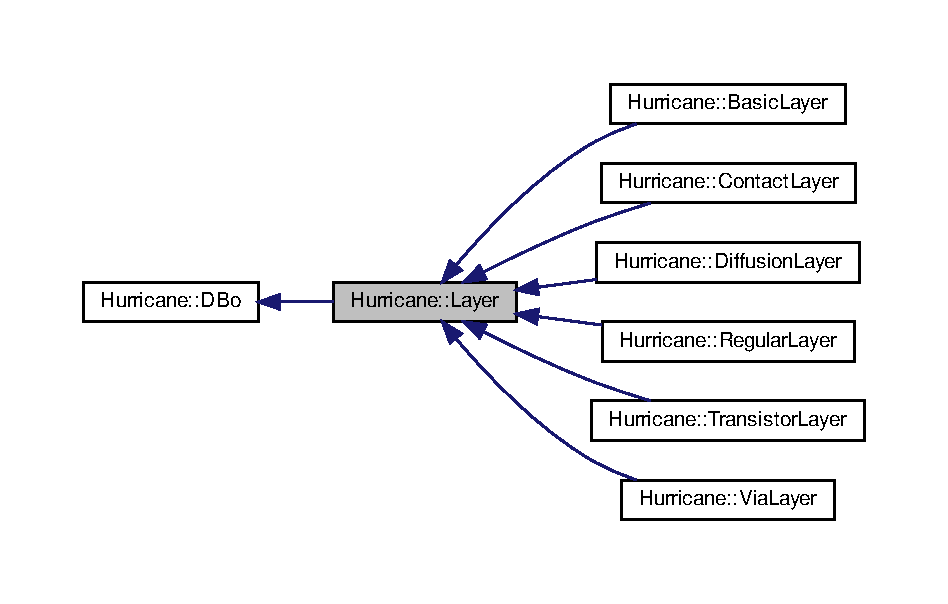
\includegraphics[width=350pt]{classHurricane_1_1Layer__inherit__graph}
\end{center}
\end{figure}
\doxysubsection*{Public Types}
\begin{DoxyCompactItemize}
\item 
typedef Hurricane\+::\+Mask$<$ unsigned long long $>$ \mbox{\hyperlink{classHurricane_1_1Layer_af5277c670637bd5d910237e7afe01a91}{Mask}}
\end{DoxyCompactItemize}
\doxysubsection*{Public Member Functions}
\begin{DoxyCompactItemize}
\item 
\mbox{\hyperlink{classHurricane_1_1Technology}{Technology}} $\ast$ \mbox{\hyperlink{classHurricane_1_1Layer_ae506b17bd7a245de622f8a8e9947629b}{get\+Technology}} () const
\item 
const \mbox{\hyperlink{classHurricane_1_1Name}{Name}} \& \mbox{\hyperlink{classHurricane_1_1Layer_a3dc54f6efc60fddb8529599caa6b0f1f}{get\+Name}} () const
\item 
const \mbox{\hyperlink{classHurricane_1_1Layer_af5277c670637bd5d910237e7afe01a91}{Mask}} \& \mbox{\hyperlink{classHurricane_1_1Layer_a29b22c3b59cc24bf82449ad6c068ff1f}{get\+Mask}} () const
\item 
const \mbox{\hyperlink{classHurricane_1_1Layer_af5277c670637bd5d910237e7afe01a91}{Mask}} \& \mbox{\hyperlink{classHurricane_1_1Layer_af009bbd89a8e8260122b7244bfa10349}{get\+Extract\+Mask}} () const
\item 
const \mbox{\hyperlink{classHurricane_1_1DbU_a4fbfa3e8c89347af76c9628ea06c4146}{Db\+U\+::\+Unit}} \& \mbox{\hyperlink{classHurricane_1_1Layer_afed9a488bf20daaeed18874f2b16268e}{get\+Minimal\+Size}} () const
\item 
const \mbox{\hyperlink{classHurricane_1_1DbU_a4fbfa3e8c89347af76c9628ea06c4146}{Db\+U\+::\+Unit}} \& \mbox{\hyperlink{classHurricane_1_1Layer_a6a03f9f40ca855d33763497162414062}{get\+Minimal\+Spacing}} () const
\item 
virtual Basic\+Layers \mbox{\hyperlink{classHurricane_1_1Layer_a7e953c126a02952e3a0b0d32f37e2ae0}{get\+Basic\+Layers}} () const =0
\item 
virtual const \mbox{\hyperlink{classHurricane_1_1Layer}{Layer}} $\ast$ \mbox{\hyperlink{classHurricane_1_1Layer_a5f7c43a29f3dd02a9ebccbcbf91d6727}{get\+Top}} () const
\item 
virtual const \mbox{\hyperlink{classHurricane_1_1Layer}{Layer}} $\ast$ \mbox{\hyperlink{classHurricane_1_1Layer_a4dab4552a219d2d900ed0b1245dc6580}{get\+Bottom}} () const
\item 
virtual const \mbox{\hyperlink{classHurricane_1_1Layer}{Layer}} $\ast$ \mbox{\hyperlink{classHurricane_1_1Layer_a69e76c09a56260169c4f5c145a35a47f}{get\+Opposite}} (const \mbox{\hyperlink{classHurricane_1_1Layer}{Layer}} $\ast$) const
\item 
\mbox{\hyperlink{classHurricane_1_1Layer}{Layer}} $\ast$ \mbox{\hyperlink{classHurricane_1_1Layer_ac32eff2dc51180660fe9b4ce17cae42c}{get\+Metal\+Above}} (bool use\+Symbolic=true) const
\item 
\mbox{\hyperlink{classHurricane_1_1Layer}{Layer}} $\ast$ \mbox{\hyperlink{classHurricane_1_1Layer_a4bc8358f67c1a1a9b2581e4b3732108c}{get\+Metal\+Below}} (bool use\+Symbolic=true) const
\item 
\mbox{\hyperlink{classHurricane_1_1Layer}{Layer}} $\ast$ \mbox{\hyperlink{classHurricane_1_1Layer_ad9fca94fed1837e3e80e9b6445822b7d}{get\+Cut\+Above}} (bool use\+Symbolic=true) const
\item 
\mbox{\hyperlink{classHurricane_1_1Layer}{Layer}} $\ast$ \mbox{\hyperlink{classHurricane_1_1Layer_a983956c8127688390f978cc5bd0d768d}{get\+Cut\+Below}} (bool use\+Symbolic=true) const
\item 
bool \mbox{\hyperlink{classHurricane_1_1Layer_abbd13bf66cf75dd6445d0353987119f3}{above}} (const \mbox{\hyperlink{classHurricane_1_1Layer}{Layer}} $\ast$layer) const
\item 
bool \mbox{\hyperlink{classHurricane_1_1Layer_a090f8697946f721351a626052af25027}{below}} (const \mbox{\hyperlink{classHurricane_1_1Layer}{Layer}} $\ast$layer) const
\item 
bool \mbox{\hyperlink{classHurricane_1_1Layer_af63dd0a48e2a3514a1cdaccd4586bad8}{contains}} (const \mbox{\hyperlink{classHurricane_1_1Layer}{Layer}} $\ast$layer) const
\item 
bool \mbox{\hyperlink{classHurricane_1_1Layer_adbea0bafaa87b033efdaa98bf2709182}{intersect}} (const \mbox{\hyperlink{classHurricane_1_1Layer}{Layer}} $\ast$layer) const
\item 
void \mbox{\hyperlink{classHurricane_1_1Layer_ab93809f19bc360f58d35e91438ef2f87}{set\+Name}} (const \mbox{\hyperlink{classHurricane_1_1Name}{Name}} \&name)
\item 
void \mbox{\hyperlink{classHurricane_1_1Layer_a400d17fe999c0080bb50489948986fe7}{set\+Minimal\+Size}} (const \mbox{\hyperlink{classHurricane_1_1DbU_a4fbfa3e8c89347af76c9628ea06c4146}{Db\+U\+::\+Unit}} \&minimal\+Size)
\item 
void \mbox{\hyperlink{classHurricane_1_1Layer_a81a8a24526e8535fba5a35cdcc194a8f}{set\+Minimal\+Spacing}} (const \mbox{\hyperlink{classHurricane_1_1DbU_a4fbfa3e8c89347af76c9628ea06c4146}{Db\+U\+::\+Unit}} \&minimal\+Spacing)
\item 
virtual void \mbox{\hyperlink{classHurricane_1_1Layer_a04e9c983525d074508d7e10107c1c3c7}{set\+Enclosure}} (const \mbox{\hyperlink{classHurricane_1_1BasicLayer}{Basic\+Layer}} $\ast$layer, \mbox{\hyperlink{classHurricane_1_1DbU_a4fbfa3e8c89347af76c9628ea06c4146}{Db\+U\+::\+Unit}}, uint32\+\_\+t flags)
\item 
virtual void \mbox{\hyperlink{classHurricane_1_1Layer_a55c7b39e000442ea36a0774d26b7fbde}{set\+Extention\+Cap}} (const \mbox{\hyperlink{classHurricane_1_1BasicLayer}{Basic\+Layer}} $\ast$layer, \mbox{\hyperlink{classHurricane_1_1DbU_a4fbfa3e8c89347af76c9628ea06c4146}{Db\+U\+::\+Unit}})
\item 
virtual void \mbox{\hyperlink{classHurricane_1_1Layer_a7a6943dbcb3403aff34056cd5de00e66}{set\+Extention\+Width}} (const \mbox{\hyperlink{classHurricane_1_1BasicLayer}{Basic\+Layer}} $\ast$layer, \mbox{\hyperlink{classHurricane_1_1DbU_a4fbfa3e8c89347af76c9628ea06c4146}{Db\+U\+::\+Unit}})
\end{DoxyCompactItemize}


\doxysubsection{Detailed Description}
\mbox{\hyperlink{classHurricane_1_1Layer}{Layer}} description ({\bfseries{API}}) 

\hypertarget{classHurricane_1_1Layer_secLayerIntro}{}\doxysubsection{Introduction}\label{classHurricane_1_1Layer_secLayerIntro}
Layers are divideds in three categories\+: 
\begin{DoxyItemize}
\item \mbox{\hyperlink{classHurricane_1_1Layer}{Layer}} \+: the base class, it supplies a generic interface sufficent for most manipulations. However, there are cases when a specific derived class may be needed. Mostly when assembling the symbolic layers. 
\item \mbox{\hyperlink{classHurricane_1_1BasicLayer}{Basic\+Layer}} \+: they represents the real process layers (GDS ones). They possesses the following characteristics\+: 
\begin{DoxyItemize}
\item Each \mbox{\hyperlink{classHurricane_1_1BasicLayer}{Basic\+Layer}} is associated with an unique bit in the \mbox{\hyperlink{classHurricane_1_1Layer_af5277c670637bd5d910237e7afe01a91}{Layer\+::\+Mask}}. This bit is used to find if a symbolic layer contains that particular \mbox{\hyperlink{classHurricane_1_1BasicLayer}{Basic\+Layer}}. 
\item No dimension extentions. Database objects drawn with those layers have rectangles the exact size specified by the user. This is mandatory if you want to create a real layout (by opposition to a symbolic one). 
\item They have a {\bfseries{material}} field hinting the purpose of the layer (is a routing metal, a cut, a diffusion and so on). 
\item They may have an associated blockage layer (for routing layers). 
\end{DoxyItemize}
\item {\bfseries{Symbolic Layers}} \+: used to draw the various components of a symbolic layout. They are made of a list of Basic\+Layers and how to extend their dimensions from the user specified sizes. 
\begin{DoxyItemize}
\item \mbox{\hyperlink{classHurricane_1_1RegularLayer}{Regular\+Layer}} \+: contains one \mbox{\hyperlink{classHurricane_1_1BasicLayer}{Basic\+Layer}}, use for wires. 
\item \mbox{\hyperlink{classHurricane_1_1ViaLayer}{Via\+Layer}} \+: contains three \mbox{\hyperlink{classHurricane_1_1BasicLayer}{Basic\+Layer}}, for contact between metal layers. The Basic\+Layers must be of {\ttfamily }(metal,cut,metal) materials. 
\item \mbox{\hyperlink{classHurricane_1_1ContactLayer}{Contact\+Layer}} \+: contains four or five Basic\+Layers, for contact towards active layers or transistor gates. The fifth optional parameter is the well. Materials of the components must be of type {\ttfamily }(metal,cut,active,diffusion\mbox{[},well\mbox{]}) 
\item \mbox{\hyperlink{classHurricane_1_1DiffusionLayer}{Diffusion\+Layer}} \+: contains three \mbox{\hyperlink{classHurricane_1_1BasicLayer}{Basic\+Layer}}, for diffusion area. Materials of the components must be of type {\ttfamily }(active,diffusion,well). 
\item \mbox{\hyperlink{classHurricane_1_1TransistorLayer}{Transistor\+Layer}} \+: contains three to four layers, for representing digital transistors. Materials are of type \+: {\ttfamily }(gate,active,diffusion,well). 
\end{DoxyItemize}
\end{DoxyItemize}

Like for the \mbox{\hyperlink{classHurricane_1_1Technology}{Technology}} object, a layer must not be deleted, else all components located on it will have a dangling pointer to an deleted object ...\hypertarget{classHurricane_1_1Layer_secBasicLayerOrder}{}\doxysubsubsection{Basic\+Layer Creation Ordering}\label{classHurricane_1_1Layer_secBasicLayerOrder}
The creation order is significant regarding the metal connectivity. The metal \& cut layers must be created in alternately fashion, for example\+: \begin{center} \tabulinesep=1mm
\begin{longtabu}spread 0pt [c]{*{3}{|X[-1]}|}
\hline
\cellcolor{\tableheadbgcolor}\textbf{ \mbox{\hyperlink{classHurricane_1_1BasicLayer}{Basic\+Layer}}}&\cellcolor{\tableheadbgcolor}\textbf{ Material}&\cellcolor{\tableheadbgcolor}\textbf{ \mbox{\hyperlink{classHurricane_1_1Layer_af5277c670637bd5d910237e7afe01a91}{Layer\+::\+Mask}} }\\\cline{1-3}
\endfirsthead
\hline
\endfoot
\hline
\cellcolor{\tableheadbgcolor}\textbf{ \mbox{\hyperlink{classHurricane_1_1BasicLayer}{Basic\+Layer}}}&\cellcolor{\tableheadbgcolor}\textbf{ Material}&\cellcolor{\tableheadbgcolor}\textbf{ \mbox{\hyperlink{classHurricane_1_1Layer_af5277c670637bd5d910237e7afe01a91}{Layer\+::\+Mask}} }\\\cline{1-3}
\endhead
{\ttfamily cut0} &\cellcolor{\tableheadbgcolor}\textbf{ {\ttfamily cut} }&\cellcolor{\tableheadbgcolor}\textbf{ {\ttfamily 0x00000010} }\\\cline{1-3}
{\ttfamily metal1} &\cellcolor{\tableheadbgcolor}\textbf{ {\ttfamily metal} }&\cellcolor{\tableheadbgcolor}\textbf{ {\ttfamily 0x00000020} }\\\cline{1-3}
{\ttfamily cut1} &\cellcolor{\tableheadbgcolor}\textbf{ {\ttfamily cut} }&\cellcolor{\tableheadbgcolor}\textbf{ {\ttfamily 0x00000040} }\\\cline{1-3}
{\ttfamily metal2} &\cellcolor{\tableheadbgcolor}\textbf{ {\ttfamily metal} }&\cellcolor{\tableheadbgcolor}\textbf{ {\ttfamily 0x00000080} }\\\cline{1-3}
{\ttfamily cut2} &\cellcolor{\tableheadbgcolor}\textbf{ {\ttfamily cut} }&\cellcolor{\tableheadbgcolor}\textbf{ {\ttfamily 0x00000100} }\\\cline{1-3}
{\ttfamily metal3} &\cellcolor{\tableheadbgcolor}\textbf{ {\ttfamily metal} }&\cellcolor{\tableheadbgcolor}\textbf{ {\ttfamily 0x00000200} }\\\cline{1-3}
\end{longtabu}
\end{center} \hypertarget{classHurricane_1_1Layer_secLayerLookup}{}\doxysubsubsection{Looking Up a Layer from a Mask}\label{classHurricane_1_1Layer_secLayerLookup}
A \mbox{\hyperlink{classHurricane_1_1BasicLayer}{Basic\+Layer}} is uniquely associated to a bit in the \mbox{\hyperlink{classHurricane_1_1Layer_af5277c670637bd5d910237e7afe01a91}{Layer\+::\+Mask}}. But, multiple symbolic layers could be built over that \mbox{\hyperlink{classHurricane_1_1BasicLayer}{Basic\+Layer}}. In that case all those layers will have the same mask. For the mask lookup functions not to be confused, we introduce the concept of {\bfseries{working layer}} in all the symbolic layers with the same mask, this is the one that will be returned. 

\doxysubsection{Member Typedef Documentation}
\mbox{\Hypertarget{classHurricane_1_1Layer_af5277c670637bd5d910237e7afe01a91}\label{classHurricane_1_1Layer_af5277c670637bd5d910237e7afe01a91}} 
\index{Hurricane::Layer@{Hurricane::Layer}!Mask@{Mask}}
\index{Mask@{Mask}!Hurricane::Layer@{Hurricane::Layer}}
\doxysubsubsection{\texorpdfstring{Mask}{Mask}}
{\footnotesize\ttfamily \mbox{\hyperlink{classHurricane_1_1Layer_af5277c670637bd5d910237e7afe01a91}{Hurricane\+::\+Layer\+::\+Mask}}}

This type represents a mask bit field characterising efficiently the constituents of any kind of layer. It associates to each basic layer a bit and to each symbolic layer the union of the bits corresponding to its basic layers. 

\doxysubsection{Member Function Documentation}
\mbox{\Hypertarget{classHurricane_1_1Layer_ae506b17bd7a245de622f8a8e9947629b}\label{classHurricane_1_1Layer_ae506b17bd7a245de622f8a8e9947629b}} 
\index{Hurricane::Layer@{Hurricane::Layer}!getTechnology@{getTechnology}}
\index{getTechnology@{getTechnology}!Hurricane::Layer@{Hurricane::Layer}}
\doxysubsubsection{\texorpdfstring{getTechnology()}{getTechnology()}}
{\footnotesize\ttfamily \mbox{\hyperlink{classHurricane_1_1Technology}{Technology}} $\ast$ Hurricane\+::\+Layer\+::get\+Technology (\begin{DoxyParamCaption}{ }\end{DoxyParamCaption}) const\hspace{0.3cm}{\ttfamily [inline]}}

{\bfseries{Returns\+:}} the technolgy owning the layer. \mbox{\Hypertarget{classHurricane_1_1Layer_a3dc54f6efc60fddb8529599caa6b0f1f}\label{classHurricane_1_1Layer_a3dc54f6efc60fddb8529599caa6b0f1f}} 
\index{Hurricane::Layer@{Hurricane::Layer}!getName@{getName}}
\index{getName@{getName}!Hurricane::Layer@{Hurricane::Layer}}
\doxysubsubsection{\texorpdfstring{getName()}{getName()}}
{\footnotesize\ttfamily const \mbox{\hyperlink{classHurricane_1_1Name}{Name}} \& Hurricane\+::\+Layer\+::get\+Name (\begin{DoxyParamCaption}{ }\end{DoxyParamCaption}) const\hspace{0.3cm}{\ttfamily [inline]}}

{\bfseries{Returns\+:}} the name of the layer. \mbox{\Hypertarget{classHurricane_1_1Layer_a29b22c3b59cc24bf82449ad6c068ff1f}\label{classHurricane_1_1Layer_a29b22c3b59cc24bf82449ad6c068ff1f}} 
\index{Hurricane::Layer@{Hurricane::Layer}!getMask@{getMask}}
\index{getMask@{getMask}!Hurricane::Layer@{Hurricane::Layer}}
\doxysubsubsection{\texorpdfstring{getMask()}{getMask()}}
{\footnotesize\ttfamily const \mbox{\hyperlink{classHurricane_1_1Layer_af5277c670637bd5d910237e7afe01a91}{Layer\+::\+Mask}} \& Hurricane\+::\+Layer\+::get\+Mask (\begin{DoxyParamCaption}{ }\end{DoxyParamCaption}) const\hspace{0.3cm}{\ttfamily [inline]}}

{\bfseries{Returns\+:}} the mask associated to the layer. 

Referenced by above(), below(), and Hurricane\+::\+Technology\+::is\+Metal().

\mbox{\Hypertarget{classHurricane_1_1Layer_af009bbd89a8e8260122b7244bfa10349}\label{classHurricane_1_1Layer_af009bbd89a8e8260122b7244bfa10349}} 
\index{Hurricane::Layer@{Hurricane::Layer}!getExtractMask@{getExtractMask}}
\index{getExtractMask@{getExtractMask}!Hurricane::Layer@{Hurricane::Layer}}
\doxysubsubsection{\texorpdfstring{getExtractMask()}{getExtractMask()}}
{\footnotesize\ttfamily const \mbox{\hyperlink{classHurricane_1_1Layer_af5277c670637bd5d910237e7afe01a91}{Layer\+::\+Mask}} \& Hurricane\+::\+Layer\+::get\+Extract\+Mask (\begin{DoxyParamCaption}{ }\end{DoxyParamCaption}) const\hspace{0.3cm}{\ttfamily [inline]}}

{\bfseries{Returns\+:}} the mask used for extraction.

Two differents basic layers have different masks but may have same extraction masks (ie CP layer which represent poly and CPG which represent poly used to realize transistor gates). \mbox{\Hypertarget{classHurricane_1_1Layer_afed9a488bf20daaeed18874f2b16268e}\label{classHurricane_1_1Layer_afed9a488bf20daaeed18874f2b16268e}} 
\index{Hurricane::Layer@{Hurricane::Layer}!getMinimalSize@{getMinimalSize}}
\index{getMinimalSize@{getMinimalSize}!Hurricane::Layer@{Hurricane::Layer}}
\doxysubsubsection{\texorpdfstring{getMinimalSize()}{getMinimalSize()}}
{\footnotesize\ttfamily const \mbox{\hyperlink{classHurricane_1_1DbU_a4fbfa3e8c89347af76c9628ea06c4146}{Db\+U\+::\+Unit}} \& Hurricane\+::\+Layer\+::get\+Minimal\+Size (\begin{DoxyParamCaption}{ }\end{DoxyParamCaption}) const\hspace{0.3cm}{\ttfamily [inline]}}

{\bfseries{Returns\+:}} the minimal size allowed for a rectangular layout pad on this layer. \mbox{\Hypertarget{classHurricane_1_1Layer_a6a03f9f40ca855d33763497162414062}\label{classHurricane_1_1Layer_a6a03f9f40ca855d33763497162414062}} 
\index{Hurricane::Layer@{Hurricane::Layer}!getMinimalSpacing@{getMinimalSpacing}}
\index{getMinimalSpacing@{getMinimalSpacing}!Hurricane::Layer@{Hurricane::Layer}}
\doxysubsubsection{\texorpdfstring{getMinimalSpacing()}{getMinimalSpacing()}}
{\footnotesize\ttfamily const \mbox{\hyperlink{classHurricane_1_1DbU_a4fbfa3e8c89347af76c9628ea06c4146}{Db\+U\+::\+Unit}} \& Hurricane\+::\+Layer\+::get\+Minimal\+Spacing (\begin{DoxyParamCaption}{ }\end{DoxyParamCaption}) const\hspace{0.3cm}{\ttfamily [inline]}}

{\bfseries{Returns\+:}} the minimal spacing between two pads on this layer. \mbox{\Hypertarget{classHurricane_1_1Layer_a7e953c126a02952e3a0b0d32f37e2ae0}\label{classHurricane_1_1Layer_a7e953c126a02952e3a0b0d32f37e2ae0}} 
\index{Hurricane::Layer@{Hurricane::Layer}!getBasicLayers@{getBasicLayers}}
\index{getBasicLayers@{getBasicLayers}!Hurricane::Layer@{Hurricane::Layer}}
\doxysubsubsection{\texorpdfstring{getBasicLayers()}{getBasicLayers()}}
{\footnotesize\ttfamily Basic\+Layers Hurricane\+::\+Layer\+::get\+Basic\+Layers (\begin{DoxyParamCaption}{ }\end{DoxyParamCaption}) const\hspace{0.3cm}{\ttfamily [pure virtual]}}

{\bfseries{Returns\+:}} the collection of basic layers within this layer.

\begin{DoxyRemark}{Remarks}
For a basic layer the collection contains this one only. 
\end{DoxyRemark}
\mbox{\Hypertarget{classHurricane_1_1Layer_a5f7c43a29f3dd02a9ebccbcbf91d6727}\label{classHurricane_1_1Layer_a5f7c43a29f3dd02a9ebccbcbf91d6727}} 
\index{Hurricane::Layer@{Hurricane::Layer}!getTop@{getTop}}
\index{getTop@{getTop}!Hurricane::Layer@{Hurricane::Layer}}
\doxysubsubsection{\texorpdfstring{getTop()}{getTop()}}
{\footnotesize\ttfamily const \mbox{\hyperlink{classHurricane_1_1Layer}{Layer}} $\ast$ Hurricane\+::\+Layer\+::get\+Top (\begin{DoxyParamCaption}{ }\end{DoxyParamCaption}) const\hspace{0.3cm}{\ttfamily [virtual]}}

{\bfseries{Returns\+:}} The uppermost layer of that layer. On \mbox{\hyperlink{classHurricane_1_1BasicLayer}{Basic\+Layer}}, it is always the layer itself. In symbolic layers the meaning depends on the object structure.

\begin{DoxyRemark}{Remarks}
In symbolic layers, top \& bottom are not related to the \mbox{\hyperlink{classHurricane_1_1Layer_af5277c670637bd5d910237e7afe01a91}{Layer\+::\+Mask}} but to the {\itshape structuration} of the layer. It is advisable that the designer create layers and symbolic layers in way that ensure the top layer is indeed the one with the greater mask. 
\end{DoxyRemark}
\mbox{\Hypertarget{classHurricane_1_1Layer_a4dab4552a219d2d900ed0b1245dc6580}\label{classHurricane_1_1Layer_a4dab4552a219d2d900ed0b1245dc6580}} 
\index{Hurricane::Layer@{Hurricane::Layer}!getBottom@{getBottom}}
\index{getBottom@{getBottom}!Hurricane::Layer@{Hurricane::Layer}}
\doxysubsubsection{\texorpdfstring{getBottom()}{getBottom()}}
{\footnotesize\ttfamily const \mbox{\hyperlink{classHurricane_1_1Layer}{Layer}} $\ast$ Hurricane\+::\+Layer\+::get\+Bottom (\begin{DoxyParamCaption}{ }\end{DoxyParamCaption}) const\hspace{0.3cm}{\ttfamily [virtual]}}

{\bfseries{Returns\+:}} The lowermost layer of that layer. On \mbox{\hyperlink{classHurricane_1_1BasicLayer}{Basic\+Layer}}, it is always the layer itself. In symbolic layers the meaning depends on the object structure. \mbox{\Hypertarget{classHurricane_1_1Layer_a69e76c09a56260169c4f5c145a35a47f}\label{classHurricane_1_1Layer_a69e76c09a56260169c4f5c145a35a47f}} 
\index{Hurricane::Layer@{Hurricane::Layer}!getOpposite@{getOpposite}}
\index{getOpposite@{getOpposite}!Hurricane::Layer@{Hurricane::Layer}}
\doxysubsubsection{\texorpdfstring{getOpposite()}{getOpposite()}}
{\footnotesize\ttfamily const \mbox{\hyperlink{classHurricane_1_1Layer}{Layer}} $\ast$ Hurricane\+::\+Layer\+::get\+Opposite (\begin{DoxyParamCaption}\item[{const \mbox{\hyperlink{classHurricane_1_1Layer}{Layer}} $\ast$}]{source }\end{DoxyParamCaption}) const\hspace{0.3cm}{\ttfamily [virtual]}}

{\bfseries{Returns\+:}} This method is only meaningful for \mbox{\hyperlink{classHurricane_1_1ViaLayer}{Via\+Layer}}. It returns the metal \mbox{\hyperlink{classHurricane_1_1Layer}{Layer}} opposite to the one given in arguments. \mbox{\Hypertarget{classHurricane_1_1Layer_ac32eff2dc51180660fe9b4ce17cae42c}\label{classHurricane_1_1Layer_ac32eff2dc51180660fe9b4ce17cae42c}} 
\index{Hurricane::Layer@{Hurricane::Layer}!getMetalAbove@{getMetalAbove}}
\index{getMetalAbove@{getMetalAbove}!Hurricane::Layer@{Hurricane::Layer}}
\doxysubsubsection{\texorpdfstring{getMetalAbove()}{getMetalAbove()}}
{\footnotesize\ttfamily \mbox{\hyperlink{classHurricane_1_1Layer}{Layer}} $\ast$ Hurricane\+::\+Layer\+::get\+Metal\+Above (\begin{DoxyParamCaption}\item[{bool}]{use\+Symbolic = {\ttfamily true} }\end{DoxyParamCaption}) const}

{\bfseries{Returns\+:}} The metal {\itshape working layer} whose mask is immediatly above this one. \mbox{\Hypertarget{classHurricane_1_1Layer_a4bc8358f67c1a1a9b2581e4b3732108c}\label{classHurricane_1_1Layer_a4bc8358f67c1a1a9b2581e4b3732108c}} 
\index{Hurricane::Layer@{Hurricane::Layer}!getMetalBelow@{getMetalBelow}}
\index{getMetalBelow@{getMetalBelow}!Hurricane::Layer@{Hurricane::Layer}}
\doxysubsubsection{\texorpdfstring{getMetalBelow()}{getMetalBelow()}}
{\footnotesize\ttfamily \mbox{\hyperlink{classHurricane_1_1Layer}{Layer}} $\ast$ Hurricane\+::\+Layer\+::get\+Metal\+Below (\begin{DoxyParamCaption}\item[{bool}]{use\+Symbolic = {\ttfamily true} }\end{DoxyParamCaption}) const}

{\bfseries{Returns\+:}} The metal {\itshape working layer} whose mask is immediatly below this one. \mbox{\Hypertarget{classHurricane_1_1Layer_ad9fca94fed1837e3e80e9b6445822b7d}\label{classHurricane_1_1Layer_ad9fca94fed1837e3e80e9b6445822b7d}} 
\index{Hurricane::Layer@{Hurricane::Layer}!getCutAbove@{getCutAbove}}
\index{getCutAbove@{getCutAbove}!Hurricane::Layer@{Hurricane::Layer}}
\doxysubsubsection{\texorpdfstring{getCutAbove()}{getCutAbove()}}
{\footnotesize\ttfamily \mbox{\hyperlink{classHurricane_1_1Layer}{Layer}} $\ast$ Hurricane\+::\+Layer\+::get\+Cut\+Above (\begin{DoxyParamCaption}\item[{bool}]{use\+Symbolic = {\ttfamily true} }\end{DoxyParamCaption}) const}

{\bfseries{Returns\+:}} The cut {\itshape working layer} whose mask is immediatly above this one. \mbox{\Hypertarget{classHurricane_1_1Layer_a983956c8127688390f978cc5bd0d768d}\label{classHurricane_1_1Layer_a983956c8127688390f978cc5bd0d768d}} 
\index{Hurricane::Layer@{Hurricane::Layer}!getCutBelow@{getCutBelow}}
\index{getCutBelow@{getCutBelow}!Hurricane::Layer@{Hurricane::Layer}}
\doxysubsubsection{\texorpdfstring{getCutBelow()}{getCutBelow()}}
{\footnotesize\ttfamily \mbox{\hyperlink{classHurricane_1_1Layer}{Layer}} $\ast$ Hurricane\+::\+Layer\+::get\+Cut\+Below (\begin{DoxyParamCaption}\item[{bool}]{use\+Symbolic = {\ttfamily true} }\end{DoxyParamCaption}) const}

{\bfseries{Returns\+:}} The cut {\itshape working layer} whose mask is immediatly below this one. \mbox{\Hypertarget{classHurricane_1_1Layer_abbd13bf66cf75dd6445d0353987119f3}\label{classHurricane_1_1Layer_abbd13bf66cf75dd6445d0353987119f3}} 
\index{Hurricane::Layer@{Hurricane::Layer}!above@{above}}
\index{above@{above}!Hurricane::Layer@{Hurricane::Layer}}
\doxysubsubsection{\texorpdfstring{above()}{above()}}
{\footnotesize\ttfamily bool Hurricane\+::\+Layer\+::above (\begin{DoxyParamCaption}\item[{const \mbox{\hyperlink{classHurricane_1_1Layer}{Layer}} $\ast$}]{layer }\end{DoxyParamCaption}) const\hspace{0.3cm}{\ttfamily [inline]}}

{\bfseries{Returns\+:}} {\bfseries{true}}, if {\ttfamily layer} is above this one. 

References get\+Mask().

\mbox{\Hypertarget{classHurricane_1_1Layer_a090f8697946f721351a626052af25027}\label{classHurricane_1_1Layer_a090f8697946f721351a626052af25027}} 
\index{Hurricane::Layer@{Hurricane::Layer}!below@{below}}
\index{below@{below}!Hurricane::Layer@{Hurricane::Layer}}
\doxysubsubsection{\texorpdfstring{below()}{below()}}
{\footnotesize\ttfamily bool Hurricane\+::\+Layer\+::below (\begin{DoxyParamCaption}\item[{const \mbox{\hyperlink{classHurricane_1_1Layer}{Layer}} $\ast$}]{layer }\end{DoxyParamCaption}) const\hspace{0.3cm}{\ttfamily [inline]}}

{\bfseries{Returns\+:}} {\bfseries{true}}, if {\ttfamily layer} is below this one. 

References get\+Mask().

\mbox{\Hypertarget{classHurricane_1_1Layer_af63dd0a48e2a3514a1cdaccd4586bad8}\label{classHurricane_1_1Layer_af63dd0a48e2a3514a1cdaccd4586bad8}} 
\index{Hurricane::Layer@{Hurricane::Layer}!contains@{contains}}
\index{contains@{contains}!Hurricane::Layer@{Hurricane::Layer}}
\doxysubsubsection{\texorpdfstring{contains()}{contains()}}
{\footnotesize\ttfamily bool Hurricane\+::\+Layer\+::contains (\begin{DoxyParamCaption}\item[{const \mbox{\hyperlink{classHurricane_1_1Layer}{Layer}} $\ast$}]{layer }\end{DoxyParamCaption}) const}

{\bfseries{Returns\+:}} {\bfseries{true}} if the {\ttfamily $<$layer$>$} is completely included in the layer {\ttfamily $<$this$>$} (that is if the basic layers of {\ttfamily $<$layer$>$} are a sub-\/set of the basic layers of {\ttfamily $<$this$>$}), else {\bfseries{false}}. \mbox{\Hypertarget{classHurricane_1_1Layer_adbea0bafaa87b033efdaa98bf2709182}\label{classHurricane_1_1Layer_adbea0bafaa87b033efdaa98bf2709182}} 
\index{Hurricane::Layer@{Hurricane::Layer}!intersect@{intersect}}
\index{intersect@{intersect}!Hurricane::Layer@{Hurricane::Layer}}
\doxysubsubsection{\texorpdfstring{intersect()}{intersect()}}
{\footnotesize\ttfamily bool Hurricane\+::\+Layer\+::intersect (\begin{DoxyParamCaption}\item[{const \mbox{\hyperlink{classHurricane_1_1Layer}{Layer}} $\ast$}]{layer }\end{DoxyParamCaption}) const}

{\bfseries{Returns\+:}} {\bfseries{true}} if the {\ttfamily $<$layer$>$} and the layer {\ttfamily $<$this$>$} have at least a common basic layer, else {\bfseries{false}}. \mbox{\Hypertarget{classHurricane_1_1Layer_ab93809f19bc360f58d35e91438ef2f87}\label{classHurricane_1_1Layer_ab93809f19bc360f58d35e91438ef2f87}} 
\index{Hurricane::Layer@{Hurricane::Layer}!setName@{setName}}
\index{setName@{setName}!Hurricane::Layer@{Hurricane::Layer}}
\doxysubsubsection{\texorpdfstring{setName()}{setName()}}
{\footnotesize\ttfamily void Hurricane\+::\+Layer\+::set\+Name (\begin{DoxyParamCaption}\item[{const \mbox{\hyperlink{classHurricane_1_1Name}{Name}} \&}]{name }\end{DoxyParamCaption})}

sets or changes the layer name.

\begin{DoxyRemark}{Remarks}
An exception is thrown if the name is empty or if there is an other layer with that name. 
\end{DoxyRemark}
\mbox{\Hypertarget{classHurricane_1_1Layer_a400d17fe999c0080bb50489948986fe7}\label{classHurricane_1_1Layer_a400d17fe999c0080bb50489948986fe7}} 
\index{Hurricane::Layer@{Hurricane::Layer}!setMinimalSize@{setMinimalSize}}
\index{setMinimalSize@{setMinimalSize}!Hurricane::Layer@{Hurricane::Layer}}
\doxysubsubsection{\texorpdfstring{setMinimalSize()}{setMinimalSize()}}
{\footnotesize\ttfamily void Hurricane\+::\+Layer\+::set\+Minimal\+Size (\begin{DoxyParamCaption}\item[{const \mbox{\hyperlink{classHurricane_1_1DbU_a4fbfa3e8c89347af76c9628ea06c4146}{Db\+U\+::\+Unit}} \&}]{minimal\+Size }\end{DoxyParamCaption})}

Sets the minimal size of a pad on this layer. \mbox{\Hypertarget{classHurricane_1_1Layer_a81a8a24526e8535fba5a35cdcc194a8f}\label{classHurricane_1_1Layer_a81a8a24526e8535fba5a35cdcc194a8f}} 
\index{Hurricane::Layer@{Hurricane::Layer}!setMinimalSpacing@{setMinimalSpacing}}
\index{setMinimalSpacing@{setMinimalSpacing}!Hurricane::Layer@{Hurricane::Layer}}
\doxysubsubsection{\texorpdfstring{setMinimalSpacing()}{setMinimalSpacing()}}
{\footnotesize\ttfamily void Hurricane\+::\+Layer\+::set\+Minimal\+Spacing (\begin{DoxyParamCaption}\item[{const \mbox{\hyperlink{classHurricane_1_1DbU_a4fbfa3e8c89347af76c9628ea06c4146}{Db\+U\+::\+Unit}} \&}]{minimal\+Spacing }\end{DoxyParamCaption})}

Sets the minimal spacing between two pads on this layer. \mbox{\Hypertarget{classHurricane_1_1Layer_a04e9c983525d074508d7e10107c1c3c7}\label{classHurricane_1_1Layer_a04e9c983525d074508d7e10107c1c3c7}} 
\index{Hurricane::Layer@{Hurricane::Layer}!setEnclosure@{setEnclosure}}
\index{setEnclosure@{setEnclosure}!Hurricane::Layer@{Hurricane::Layer}}
\doxysubsubsection{\texorpdfstring{setEnclosure()}{setEnclosure()}}
{\footnotesize\ttfamily void Hurricane\+::\+Layer\+::set\+Enclosure (\begin{DoxyParamCaption}\item[{const \mbox{\hyperlink{classHurricane_1_1BasicLayer}{Basic\+Layer}} $\ast$}]{layer,  }\item[{\mbox{\hyperlink{classHurricane_1_1DbU_a4fbfa3e8c89347af76c9628ea06c4146}{Db\+U\+::\+Unit}}}]{,  }\item[{uint32\+\_\+t}]{flags }\end{DoxyParamCaption})\hspace{0.3cm}{\ttfamily [virtual]}}

Sets the enclosure for the given \mbox{\hyperlink{classHurricane_1_1BasicLayer}{Basic\+Layer}}. \mbox{\Hypertarget{classHurricane_1_1Layer_a55c7b39e000442ea36a0774d26b7fbde}\label{classHurricane_1_1Layer_a55c7b39e000442ea36a0774d26b7fbde}} 
\index{Hurricane::Layer@{Hurricane::Layer}!setExtentionCap@{setExtentionCap}}
\index{setExtentionCap@{setExtentionCap}!Hurricane::Layer@{Hurricane::Layer}}
\doxysubsubsection{\texorpdfstring{setExtentionCap()}{setExtentionCap()}}
{\footnotesize\ttfamily void Hurricane\+::\+Layer\+::set\+Extention\+Cap (\begin{DoxyParamCaption}\item[{const \mbox{\hyperlink{classHurricane_1_1BasicLayer}{Basic\+Layer}} $\ast$}]{layer,  }\item[{\mbox{\hyperlink{classHurricane_1_1DbU_a4fbfa3e8c89347af76c9628ea06c4146}{Db\+U\+::\+Unit}}}]{ecap }\end{DoxyParamCaption})\hspace{0.3cm}{\ttfamily [virtual]}}

Sets the extention cap for the given \mbox{\hyperlink{classHurricane_1_1BasicLayer}{Basic\+Layer}}. \mbox{\Hypertarget{classHurricane_1_1Layer_a7a6943dbcb3403aff34056cd5de00e66}\label{classHurricane_1_1Layer_a7a6943dbcb3403aff34056cd5de00e66}} 
\index{Hurricane::Layer@{Hurricane::Layer}!setExtentionWidth@{setExtentionWidth}}
\index{setExtentionWidth@{setExtentionWidth}!Hurricane::Layer@{Hurricane::Layer}}
\doxysubsubsection{\texorpdfstring{setExtentionWidth()}{setExtentionWidth()}}
{\footnotesize\ttfamily void Hurricane\+::\+Layer\+::set\+Extention\+Width (\begin{DoxyParamCaption}\item[{const \mbox{\hyperlink{classHurricane_1_1BasicLayer}{Basic\+Layer}} $\ast$}]{layer,  }\item[{\mbox{\hyperlink{classHurricane_1_1DbU_a4fbfa3e8c89347af76c9628ea06c4146}{Db\+U\+::\+Unit}}}]{ewidth }\end{DoxyParamCaption})\hspace{0.3cm}{\ttfamily [virtual]}}

Sets the extention width for the given \mbox{\hyperlink{classHurricane_1_1BasicLayer}{Basic\+Layer}}. 

The documentation for this class was generated from the following files\+:\begin{DoxyCompactItemize}
\item 
Layer.\+h\item 
Layer.\+dox\end{DoxyCompactItemize}

\hypertarget{classHurricane_1_1Library}{}\doxysection{Hurricane\+::Library Class Reference}
\label{classHurricane_1_1Library}\index{Hurricane::Library@{Hurricane::Library}}


\mbox{\hyperlink{classHurricane_1_1Library}{Library}} description ({\bfseries{API}})  




Inheritance diagram for Hurricane\+::Library\+:\nopagebreak
\begin{figure}[H]
\begin{center}
\leavevmode
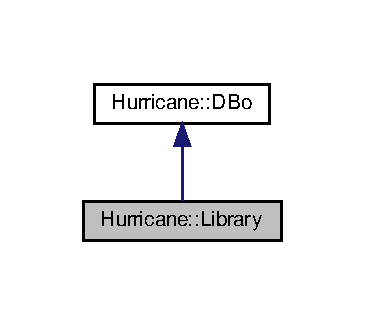
\includegraphics[width=175pt]{classHurricane_1_1Library__inherit__graph}
\end{center}
\end{figure}
\doxysubsection*{Public Types}
\begin{DoxyCompactItemize}
\item 
typedef \mbox{\hyperlink{classHurricane_1_1DBo}{DBo}} \mbox{\hyperlink{classHurricane_1_1Library_a30ef446b2da0d405bdf4e11ce67b160f}{Inherit}}
\end{DoxyCompactItemize}
\doxysubsection*{Public Member Functions}
\begin{DoxyCompactItemize}
\item 
\mbox{\hyperlink{classHurricane_1_1DataBase}{Data\+Base}} $\ast$ \mbox{\hyperlink{classHurricane_1_1Library_a657cbf1ac426ef6def0b5b51f80ed248}{get\+Data\+Base}} () const
\item 
\mbox{\hyperlink{classHurricane_1_1Library}{Library}} $\ast$ \mbox{\hyperlink{classHurricane_1_1Library_a5299d19afc96c535d557b86ba42eaa82}{get\+Library}} () const
\item 
const \mbox{\hyperlink{classHurricane_1_1Name}{Name}} \& \mbox{\hyperlink{classHurricane_1_1Library_a13a9c4d0c43e2e1df09b7c0ee59f577f}{get\+Name}} () const
\item 
\mbox{\hyperlink{classHurricane_1_1Library}{Library}} $\ast$ \mbox{\hyperlink{classHurricane_1_1Library_a8589e1ff3db5ef288c3027ceef28636b}{get\+Library}} (const \mbox{\hyperlink{classHurricane_1_1Name}{Name}} \&name) const
\item 
\mbox{\hyperlink{namespaceHurricane_a2868a53bbb0507710460ff02fab77cad}{Libraries}} \mbox{\hyperlink{classHurricane_1_1Library_a43b3703b939b7e70261d1f9319db2bb0}{get\+Libraries}} () const
\item 
\mbox{\hyperlink{classHurricane_1_1Cell}{Cell}} $\ast$ \mbox{\hyperlink{classHurricane_1_1Library_a2e6bb294c611db79e00a5a6ea00974d5}{get\+Cell}} (const \mbox{\hyperlink{classHurricane_1_1Name}{Name}} \&name) const
\item 
\mbox{\hyperlink{namespaceHurricane_a8b4ab14b26f36f43d83a50294410b44a}{Cells}} \mbox{\hyperlink{classHurricane_1_1Library_aae3e47aef08e50f9858fb79537f6eb41}{get\+Cells}} () const
\item 
void \mbox{\hyperlink{classHurricane_1_1Library_a1181e4e87f42749bdfda253cad658ea9}{set\+Name}} (const \mbox{\hyperlink{classHurricane_1_1Name}{Name}} \&name)
\end{DoxyCompactItemize}
\doxysubsection*{Static Public Member Functions}
\begin{DoxyCompactItemize}
\item 
static \mbox{\hyperlink{classHurricane_1_1Library}{Library}} $\ast$ \mbox{\hyperlink{classHurricane_1_1Library_af304234d0347128300df5ad09801229d}{create}} (\mbox{\hyperlink{classHurricane_1_1DataBase}{Data\+Base}} $\ast$data\+Base, const \mbox{\hyperlink{classHurricane_1_1Name}{Name}} \&name)
\item 
static \mbox{\hyperlink{classHurricane_1_1Library}{Library}} $\ast$ \mbox{\hyperlink{classHurricane_1_1Library_a36bc1af0e48307180be81a81d462650e}{create}} (\mbox{\hyperlink{classHurricane_1_1Library}{Library}} $\ast$library, const \mbox{\hyperlink{classHurricane_1_1Name}{Name}} \&name)
\end{DoxyCompactItemize}


\doxysubsection{Detailed Description}
\mbox{\hyperlink{classHurricane_1_1Library}{Library}} description ({\bfseries{API}}) 

\hypertarget{classHurricane_1_1Library_secLibraryIntro}{}\doxysubsection{Introduction}\label{classHurricane_1_1Library_secLibraryIntro}
A library contains a set of symbols, a set of cells and may also contains a set of sub libraries.

A root library exists directly attached to the data\+\_\+base. This root library is the only one which has no parent library. 

\doxysubsection{Member Typedef Documentation}
\mbox{\Hypertarget{classHurricane_1_1Library_a30ef446b2da0d405bdf4e11ce67b160f}\label{classHurricane_1_1Library_a30ef446b2da0d405bdf4e11ce67b160f}} 
\index{Hurricane::Library@{Hurricane::Library}!Inherit@{Inherit}}
\index{Inherit@{Inherit}!Hurricane::Library@{Hurricane::Library}}
\doxysubsubsection{\texorpdfstring{Inherit}{Inherit}}
{\footnotesize\ttfamily \mbox{\hyperlink{classHurricane_1_1Library_a30ef446b2da0d405bdf4e11ce67b160f}{Hurricane\+::\+Library\+::\+Inherit}}}

Useful for calling upon methods of the base class without knowing it. 

\doxysubsection{Member Function Documentation}
\mbox{\Hypertarget{classHurricane_1_1Library_af304234d0347128300df5ad09801229d}\label{classHurricane_1_1Library_af304234d0347128300df5ad09801229d}} 
\index{Hurricane::Library@{Hurricane::Library}!create@{create}}
\index{create@{create}!Hurricane::Library@{Hurricane::Library}}
\doxysubsubsection{\texorpdfstring{create()}{create()}\hspace{0.1cm}{\footnotesize\ttfamily [1/2]}}
{\footnotesize\ttfamily \mbox{\hyperlink{classHurricane_1_1Library}{Library}} $\ast$ Hurricane\+::\+Library\+::create (\begin{DoxyParamCaption}\item[{\mbox{\hyperlink{classHurricane_1_1DataBase}{Data\+Base}} $\ast$}]{data\+Base,  }\item[{const \mbox{\hyperlink{classHurricane_1_1Name}{Name}} \&}]{name }\end{DoxyParamCaption})\hspace{0.3cm}{\ttfamily [static]}}

creates and returns a new root library named {\ttfamily $<$name$>$} for the data base {\ttfamily $<$data\+Base$>$}.

\begin{DoxyParagraph}{Caution\+: Throws an exception if the data base is null, if the name is }
empty or if the data base already contains a root library. 
\end{DoxyParagraph}
\mbox{\Hypertarget{classHurricane_1_1Library_a36bc1af0e48307180be81a81d462650e}\label{classHurricane_1_1Library_a36bc1af0e48307180be81a81d462650e}} 
\index{Hurricane::Library@{Hurricane::Library}!create@{create}}
\index{create@{create}!Hurricane::Library@{Hurricane::Library}}
\doxysubsubsection{\texorpdfstring{create()}{create()}\hspace{0.1cm}{\footnotesize\ttfamily [2/2]}}
{\footnotesize\ttfamily \mbox{\hyperlink{classHurricane_1_1Library}{Library}} $\ast$ Hurricane\+::\+Library\+::create (\begin{DoxyParamCaption}\item[{\mbox{\hyperlink{classHurricane_1_1Library}{Library}} $\ast$}]{library,  }\item[{const \mbox{\hyperlink{classHurricane_1_1Name}{Name}} \&}]{name }\end{DoxyParamCaption})\hspace{0.3cm}{\ttfamily [static]}}

creates and returns a new sub library named {\ttfamily $<$name$>$} for the library {\ttfamily $<$library$>$}.

\begin{DoxyParagraph}{Caution\+: Throws an exception if the library is null, if the name is }
empty or if a sub library with same name already exists in the library. 
\end{DoxyParagraph}
\mbox{\Hypertarget{classHurricane_1_1Library_a657cbf1ac426ef6def0b5b51f80ed248}\label{classHurricane_1_1Library_a657cbf1ac426ef6def0b5b51f80ed248}} 
\index{Hurricane::Library@{Hurricane::Library}!getDataBase@{getDataBase}}
\index{getDataBase@{getDataBase}!Hurricane::Library@{Hurricane::Library}}
\doxysubsubsection{\texorpdfstring{getDataBase()}{getDataBase()}}
{\footnotesize\ttfamily \mbox{\hyperlink{classHurricane_1_1DataBase}{Data\+Base}} $\ast$ Hurricane\+::\+Library\+::get\+Data\+Base (\begin{DoxyParamCaption}{ }\end{DoxyParamCaption}) const\hspace{0.3cm}{\ttfamily [inline]}}

{\bfseries{Returns\+:}} the data base owning directly or indirectly the library. \mbox{\Hypertarget{classHurricane_1_1Library_a5299d19afc96c535d557b86ba42eaa82}\label{classHurricane_1_1Library_a5299d19afc96c535d557b86ba42eaa82}} 
\index{Hurricane::Library@{Hurricane::Library}!getLibrary@{getLibrary}}
\index{getLibrary@{getLibrary}!Hurricane::Library@{Hurricane::Library}}
\doxysubsubsection{\texorpdfstring{getLibrary()}{getLibrary()}\hspace{0.1cm}{\footnotesize\ttfamily [1/2]}}
{\footnotesize\ttfamily \mbox{\hyperlink{classHurricane_1_1Library}{Library}} $\ast$ Hurricane\+::\+Library\+::get\+Library (\begin{DoxyParamCaption}{ }\end{DoxyParamCaption}) const\hspace{0.3cm}{\ttfamily [inline]}}

{\bfseries{Returns\+:}} the library owning the library (NULL for the root library). \mbox{\Hypertarget{classHurricane_1_1Library_a13a9c4d0c43e2e1df09b7c0ee59f577f}\label{classHurricane_1_1Library_a13a9c4d0c43e2e1df09b7c0ee59f577f}} 
\index{Hurricane::Library@{Hurricane::Library}!getName@{getName}}
\index{getName@{getName}!Hurricane::Library@{Hurricane::Library}}
\doxysubsubsection{\texorpdfstring{getName()}{getName()}}
{\footnotesize\ttfamily const \mbox{\hyperlink{classHurricane_1_1Name}{Name}} \& Hurricane\+::\+Library\+::get\+Name (\begin{DoxyParamCaption}{ }\end{DoxyParamCaption}) const\hspace{0.3cm}{\ttfamily [inline]}}

{\bfseries{Returns\+:}} the name of the library. \mbox{\Hypertarget{classHurricane_1_1Library_a8589e1ff3db5ef288c3027ceef28636b}\label{classHurricane_1_1Library_a8589e1ff3db5ef288c3027ceef28636b}} 
\index{Hurricane::Library@{Hurricane::Library}!getLibrary@{getLibrary}}
\index{getLibrary@{getLibrary}!Hurricane::Library@{Hurricane::Library}}
\doxysubsubsection{\texorpdfstring{getLibrary()}{getLibrary()}\hspace{0.1cm}{\footnotesize\ttfamily [2/2]}}
{\footnotesize\ttfamily \mbox{\hyperlink{classHurricane_1_1Library}{Library}} $\ast$ Hurricane\+::\+Library\+::get\+Library (\begin{DoxyParamCaption}\item[{const \mbox{\hyperlink{classHurricane_1_1Name}{Name}} \&}]{name }\end{DoxyParamCaption}) const\hspace{0.3cm}{\ttfamily [inline]}}

{\bfseries{Returns\+:}} the sub library of name {\ttfamily $<$name$>$} if it exists, else NULL. \mbox{\Hypertarget{classHurricane_1_1Library_a43b3703b939b7e70261d1f9319db2bb0}\label{classHurricane_1_1Library_a43b3703b939b7e70261d1f9319db2bb0}} 
\index{Hurricane::Library@{Hurricane::Library}!getLibraries@{getLibraries}}
\index{getLibraries@{getLibraries}!Hurricane::Library@{Hurricane::Library}}
\doxysubsubsection{\texorpdfstring{getLibraries()}{getLibraries()}}
{\footnotesize\ttfamily \mbox{\hyperlink{namespaceHurricane_a2868a53bbb0507710460ff02fab77cad}{Libraries}} Hurricane\+::\+Library\+::get\+Libraries (\begin{DoxyParamCaption}{ }\end{DoxyParamCaption}) const\hspace{0.3cm}{\ttfamily [inline]}}

{\bfseries{Returns\+:}} the collection of all sub libraries of the library. \mbox{\Hypertarget{classHurricane_1_1Library_a2e6bb294c611db79e00a5a6ea00974d5}\label{classHurricane_1_1Library_a2e6bb294c611db79e00a5a6ea00974d5}} 
\index{Hurricane::Library@{Hurricane::Library}!getCell@{getCell}}
\index{getCell@{getCell}!Hurricane::Library@{Hurricane::Library}}
\doxysubsubsection{\texorpdfstring{getCell()}{getCell()}}
{\footnotesize\ttfamily \mbox{\hyperlink{classHurricane_1_1Cell}{Cell}} $\ast$ Hurricane\+::\+Library\+::get\+Cell (\begin{DoxyParamCaption}\item[{const \mbox{\hyperlink{classHurricane_1_1Name}{Name}} \&}]{name }\end{DoxyParamCaption}) const\hspace{0.3cm}{\ttfamily [inline]}}

{\bfseries{Returns\+:}} the cell of name {\ttfamily $<$name$>$} if it exists, else NULL. \mbox{\Hypertarget{classHurricane_1_1Library_aae3e47aef08e50f9858fb79537f6eb41}\label{classHurricane_1_1Library_aae3e47aef08e50f9858fb79537f6eb41}} 
\index{Hurricane::Library@{Hurricane::Library}!getCells@{getCells}}
\index{getCells@{getCells}!Hurricane::Library@{Hurricane::Library}}
\doxysubsubsection{\texorpdfstring{getCells()}{getCells()}}
{\footnotesize\ttfamily \mbox{\hyperlink{namespaceHurricane_a8b4ab14b26f36f43d83a50294410b44a}{Cells}} Hurricane\+::\+Library\+::get\+Cells (\begin{DoxyParamCaption}{ }\end{DoxyParamCaption}) const\hspace{0.3cm}{\ttfamily [inline]}}

{\bfseries{Returns\+:}} the collection of all cells of the library. \mbox{\Hypertarget{classHurricane_1_1Library_a1181e4e87f42749bdfda253cad658ea9}\label{classHurricane_1_1Library_a1181e4e87f42749bdfda253cad658ea9}} 
\index{Hurricane::Library@{Hurricane::Library}!setName@{setName}}
\index{setName@{setName}!Hurricane::Library@{Hurricane::Library}}
\doxysubsubsection{\texorpdfstring{setName()}{setName()}}
{\footnotesize\ttfamily void Hurricane\+::\+Library\+::set\+Name (\begin{DoxyParamCaption}\item[{const \mbox{\hyperlink{classHurricane_1_1Name}{Name}} \&}]{name }\end{DoxyParamCaption})}

Allows to change the library name.

\begin{DoxyRemark}{Remarks}
Throws an exception if the new name is empty or if the library owning the library (if any) has already a sub library with the same name. 
\end{DoxyRemark}


The documentation for this class was generated from the following files\+:\begin{DoxyCompactItemize}
\item 
Library.\+h\item 
Library.\+dox\end{DoxyCompactItemize}

\hypertarget{classHurricane_1_1ListCollection}{}\doxysection{Hurricane\+::List\+Collection$<$ Element $>$ Class Template Reference}
\label{classHurricane_1_1ListCollection}\index{Hurricane::ListCollection$<$ Element $>$@{Hurricane::ListCollection$<$ Element $>$}}


\mbox{\hyperlink{namespaceHurricane}{Hurricane}} \mbox{\hyperlink{classHurricane_1_1Collection}{Collection}} wrapper around a std\+::list.  




Inheritance diagram for Hurricane\+::List\+Collection$<$ Element $>$\+:\nopagebreak
\begin{figure}[H]
\begin{center}
\leavevmode
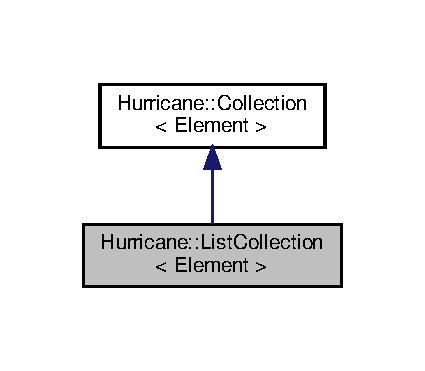
\includegraphics[width=204pt]{classHurricane_1_1ListCollection__inherit__graph}
\end{center}
\end{figure}
\doxysubsection*{Public Member Functions}
\begin{Indent}\textbf{ Collection Collection}\par
{\em \hypertarget{Collection_8h_secCollectionUtilitarians}{}\doxysubsection{Utilitarians}\label{Collection_8h_secCollectionUtilitarians}
{\bfseries{Collection\+::\+Fill}} {\bfseries{Collection\+::\+Fill}} {\bfseries{Collection\+::\+Fill}} \begin{DoxyRemark}{Remarks}
The elements are added to the container in the order with which the collection is visited. So the same order will appear in a list or a vector, but for a set they will be inserted according to the set ordering method. 
\end{DoxyRemark}
}\begin{DoxyCompactItemize}
\item 
\mbox{\hyperlink{classHurricane_1_1ListCollection_a11d0b27c9b01f16fe9ac9da091575e7c}{List\+Collection}} (const Element\+List $\ast$element\+List=NULL)
\end{DoxyCompactItemize}
\end{Indent}


\doxysubsection{Detailed Description}
\subsubsection*{template$<$class Element$>$\newline
class Hurricane\+::\+List\+Collection$<$ Element $>$}

\mbox{\hyperlink{namespaceHurricane}{Hurricane}} \mbox{\hyperlink{classHurricane_1_1Collection}{Collection}} wrapper around a std\+::list. 

Automatically wrap a \mbox{\hyperlink{namespaceHurricane}{Hurricane}} \mbox{\hyperlink{classHurricane_1_1Collection}{Collection}} around a stl\+::list. 

\doxysubsection{Constructor \& Destructor Documentation}
\mbox{\Hypertarget{classHurricane_1_1ListCollection_a11d0b27c9b01f16fe9ac9da091575e7c}\label{classHurricane_1_1ListCollection_a11d0b27c9b01f16fe9ac9da091575e7c}} 
\index{Hurricane::ListCollection$<$ Element $>$@{Hurricane::ListCollection$<$ Element $>$}!ListCollection@{ListCollection}}
\index{ListCollection@{ListCollection}!Hurricane::ListCollection$<$ Element $>$@{Hurricane::ListCollection$<$ Element $>$}}
\doxysubsubsection{\texorpdfstring{ListCollection()}{ListCollection()}}
{\footnotesize\ttfamily template$<$class Element $>$ \\
\mbox{\hyperlink{classHurricane_1_1ListCollection}{Hurricane\+::\+List\+Collection}}$<$ Element $>$\+::\mbox{\hyperlink{classHurricane_1_1ListCollection}{List\+Collection}} (\begin{DoxyParamCaption}\item[{const Element\+List $\ast$}]{element\+List = {\ttfamily NULL} }\end{DoxyParamCaption})\hspace{0.3cm}{\ttfamily [inline]}}

Constructor from a STL list, the list must not be de-\/allocated. 

The documentation for this class was generated from the following files\+:\begin{DoxyCompactItemize}
\item 
List\+Collection.\+h\item 
Collection.\+dox\end{DoxyCompactItemize}

\hypertarget{classHurricane_1_1Locator}{}\doxysection{Hurricane\+::Locator$<$ Type $>$ Class Template Reference}
\label{classHurricane_1_1Locator}\index{Hurricane::Locator$<$ Type $>$@{Hurricane::Locator$<$ Type $>$}}


\mbox{\hyperlink{classHurricane_1_1Locator}{Locator}} description ({\bfseries{API}})  




Inheritance diagram for Hurricane\+::Locator$<$ Type $>$\+:\nopagebreak
\begin{figure}[H]
\begin{center}
\leavevmode
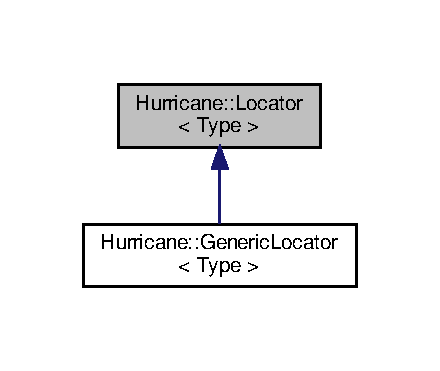
\includegraphics[width=211pt]{classHurricane_1_1Locator__inherit__graph}
\end{center}
\end{figure}
\doxysubsection*{Public Member Functions}
\begin{DoxyCompactItemize}
\item 
virtual Type \mbox{\hyperlink{classHurricane_1_1Locator_aa2202b4cf461a7c3b666da10bc96219f}{get\+Element}} () const =0
\item 
virtual \mbox{\hyperlink{classHurricane_1_1Locator}{Locator}}$<$ Type $>$ $\ast$ \mbox{\hyperlink{classHurricane_1_1Locator_a83779aa300e3de011bf3b93be8a48d83}{get\+Clone}} () const =0
\item 
virtual bool \mbox{\hyperlink{classHurricane_1_1Locator_abb6e5255372e22e31bf0a8e4cae93f87}{is\+Valid}} () const =0
\item 
virtual void \mbox{\hyperlink{classHurricane_1_1Locator_ad8d72c1625a343a50520792c96fa1ca1}{progress}} ()=0
\end{DoxyCompactItemize}


\doxysubsection{Detailed Description}
\subsubsection*{template$<$class Type$>$\newline
class Hurricane\+::\+Locator$<$ Type $>$}

\mbox{\hyperlink{classHurricane_1_1Locator}{Locator}} description ({\bfseries{API}}) 

\hypertarget{classHurricane_1_1Locator_secLocatorIntro}{}\doxysubsection{Introduction}\label{classHurricane_1_1Locator_secLocatorIntro}
Locators are objects which allow to walk efficiently through the data structure.

Locators are indeed algorithms. They do not hold a list of elements but the way to go from one element to the next. As such, they are very light in memory, contrary to containers. Locators are the workhorse of \mbox{\hyperlink{classHurricane_1_1Collection}{Collection}}, and while they can be used directly, this is not the recommended way.\hypertarget{classHurricane_1_1Locator_secLocatorGeneralConcepts}{}\doxysubsection{General concepts}\label{classHurricane_1_1Locator_secLocatorGeneralConcepts}
{\bfseries{Initialization}} In order to get a locator, you must \+: either ask the collection to provide a locator for visiting the elements of its described set, or build a clone of an existing locator allowing to visit the remaining elements starting from the current position of that locator.

{\bfseries{End of walk indicator}} The predicate {\bfseries{\mbox{\hyperlink{classHurricane_1_1Locator_abb6e5255372e22e31bf0a8e4cae93f87}{is\+Valid()}}}} returns {\bfseries{true}} if the locator refers an element of the set, {\bfseries{false}} when all the elements have been visited.

{\bfseries{getting the current element}} The current element is obtained by the accessor {\bfseries{\mbox{\hyperlink{classHurricane_1_1Locator_aa2202b4cf461a7c3b666da10bc96219f}{get\+Element()}}}}. There is no risk to call this function when the visit is finished or the locator is non initialized (the returned value is meaningless).

{\bfseries{Walk progression}} The function {\bfseries{\mbox{\hyperlink{classHurricane_1_1Locator_ad8d72c1625a343a50520792c96fa1ca1}{progress()}}}} moves forward the locator on the next element of the set (does nothing if called after the last element).\hypertarget{classHurricane_1_1Locator_secLocatorUsageExamples}{}\doxysubsection{Usage examples}\label{classHurricane_1_1Locator_secLocatorUsageExamples}
The following sample code shows how to trace the nets of a given cell 
\begin{DoxyCode}{0}
\DoxyCodeLine{Cell* cell = ...; \textcolor{comment}{// we get the cell}}
\DoxyCodeLine{ }
\DoxyCodeLine{\textcolor{keywordflow}{if} (cell) \{}
\DoxyCodeLine{ }
\DoxyCodeLine{   \textcolor{comment}{// cell-\/>getNets()}}
\DoxyCodeLine{   \textcolor{comment}{//    returns the nets collection of the cell}}
\DoxyCodeLine{   \textcolor{comment}{// and getLocator()}}
\DoxyCodeLine{   \textcolor{comment}{//    allocates and returns a locator for traversing those nets}}
\DoxyCodeLine{   Locator<Net*>* locator = cell-\/>getNets().getLocator();}
\DoxyCodeLine{ }
\DoxyCodeLine{   \textcolor{keywordflow}{while} (locator-\/>isValid()) \{}
\DoxyCodeLine{      Net* net = locator-\/>getElement();}
\DoxyCodeLine{      assert(net-\/>getCell() == cell);}
\DoxyCodeLine{      locator-\/>progress();}
\DoxyCodeLine{   \}}
\DoxyCodeLine{ }
\DoxyCodeLine{   \textcolor{comment}{// don't forget to release the allocated locator}}
\DoxyCodeLine{   \textcolor{keyword}{delete} locator;}
\DoxyCodeLine{\}}

\end{DoxyCode}
 And this one how to print all pairs of nets of a given cell 
\begin{DoxyCode}{0}
\DoxyCodeLine{Cell* cell = ...; \textcolor{comment}{// we get a cell}}
\DoxyCodeLine{ }
\DoxyCodeLine{\textcolor{keywordflow}{if} (cell) \{}
\DoxyCodeLine{   Locator<Net*>* locator1 = cell-\/>GetNets().getLocator();}
\DoxyCodeLine{   \textcolor{keywordflow}{while} (locator1-\/>isValid()) \{}
\DoxyCodeLine{      Net* net1 = locator1-\/>getElement();}
\DoxyCodeLine{ }
\DoxyCodeLine{      Locator<Net*>* locator2 = locator1-\/>getClone();}
\DoxyCodeLine{      \textcolor{keywordflow}{while} (locator2-\/>isValid()) \{}
\DoxyCodeLine{         Net* net2 = locator2-\/>getElement();}
\DoxyCodeLine{         cerr << net1 << \textcolor{stringliteral}{"{} "{}} << net2 << endl;}
\DoxyCodeLine{         locator2-\/>progress();}
\DoxyCodeLine{      \}}
\DoxyCodeLine{      \textcolor{keyword}{delete} locator2;}
\DoxyCodeLine{ }
\DoxyCodeLine{      locator1-\/>progress();}
\DoxyCodeLine{   \}}
\DoxyCodeLine{   \textcolor{keyword}{delete} locator1;}
\DoxyCodeLine{\}}

\end{DoxyCode}
 \begin{DoxyRemark}{Remarks}
Those examples are given in order to explain how locators work. We will see in the following how to do that more simply by using generic locators, or even simpler by using the for\+Each macros. 
\end{DoxyRemark}


\doxysubsection{Member Function Documentation}
\mbox{\Hypertarget{classHurricane_1_1Locator_aa2202b4cf461a7c3b666da10bc96219f}\label{classHurricane_1_1Locator_aa2202b4cf461a7c3b666da10bc96219f}} 
\index{Hurricane::Locator$<$ Type $>$@{Hurricane::Locator$<$ Type $>$}!getElement@{getElement}}
\index{getElement@{getElement}!Hurricane::Locator$<$ Type $>$@{Hurricane::Locator$<$ Type $>$}}
\doxysubsubsection{\texorpdfstring{getElement()}{getElement()}}
{\footnotesize\ttfamily template$<$class Type $>$ \\
Type \mbox{\hyperlink{classHurricane_1_1Locator}{Hurricane\+::\+Locator}}$<$ Type $>$\+::get\+Element (\begin{DoxyParamCaption}{ }\end{DoxyParamCaption}) const\hspace{0.3cm}{\ttfamily [pure virtual]}}

{\bfseries{Returns\+:}} the current element (or the value {\bfseries{Type()}} when the locator is not or no longer valid). \mbox{\Hypertarget{classHurricane_1_1Locator_a83779aa300e3de011bf3b93be8a48d83}\label{classHurricane_1_1Locator_a83779aa300e3de011bf3b93be8a48d83}} 
\index{Hurricane::Locator$<$ Type $>$@{Hurricane::Locator$<$ Type $>$}!getClone@{getClone}}
\index{getClone@{getClone}!Hurricane::Locator$<$ Type $>$@{Hurricane::Locator$<$ Type $>$}}
\doxysubsubsection{\texorpdfstring{getClone()}{getClone()}}
{\footnotesize\ttfamily template$<$class Type $>$ \\
\mbox{\hyperlink{classHurricane_1_1Locator}{Locator}}$<$ Type $>$ $\ast$ \mbox{\hyperlink{classHurricane_1_1Locator}{Hurricane\+::\+Locator}}$<$ Type $>$\+::get\+Clone (\begin{DoxyParamCaption}{ }\end{DoxyParamCaption}) const\hspace{0.3cm}{\ttfamily [pure virtual]}}

This function allocates and returns a new locator that will have the same visiting course than the remaining one of the locator being cloned.

\begin{DoxyRemark}{Remarks}
In principle there is no need to call this function, but if you do so you must not forget to release the clone after its use or, from it, build a generic locator which will do that for you (to be explained later). 
\end{DoxyRemark}
\mbox{\Hypertarget{classHurricane_1_1Locator_abb6e5255372e22e31bf0a8e4cae93f87}\label{classHurricane_1_1Locator_abb6e5255372e22e31bf0a8e4cae93f87}} 
\index{Hurricane::Locator$<$ Type $>$@{Hurricane::Locator$<$ Type $>$}!isValid@{isValid}}
\index{isValid@{isValid}!Hurricane::Locator$<$ Type $>$@{Hurricane::Locator$<$ Type $>$}}
\doxysubsubsection{\texorpdfstring{isValid()}{isValid()}}
{\footnotesize\ttfamily template$<$class Type $>$ \\
bool \mbox{\hyperlink{classHurricane_1_1Locator}{Hurricane\+::\+Locator}}$<$ Type $>$\+::is\+Valid (\begin{DoxyParamCaption}{ }\end{DoxyParamCaption}) const\hspace{0.3cm}{\ttfamily [pure virtual]}}

{\bfseries{Returns\+:}} {\bfseries{true}} while the walk has not exhausted the set of elements, else {\bfseries{false}}. \mbox{\Hypertarget{classHurricane_1_1Locator_ad8d72c1625a343a50520792c96fa1ca1}\label{classHurricane_1_1Locator_ad8d72c1625a343a50520792c96fa1ca1}} 
\index{Hurricane::Locator$<$ Type $>$@{Hurricane::Locator$<$ Type $>$}!progress@{progress}}
\index{progress@{progress}!Hurricane::Locator$<$ Type $>$@{Hurricane::Locator$<$ Type $>$}}
\doxysubsubsection{\texorpdfstring{progress()}{progress()}}
{\footnotesize\ttfamily template$<$class Type $>$ \\
void \mbox{\hyperlink{classHurricane_1_1Locator}{Hurricane\+::\+Locator}}$<$ Type $>$\+::progress (\begin{DoxyParamCaption}{ }\end{DoxyParamCaption})\hspace{0.3cm}{\ttfamily [pure virtual]}}

Moves forward the locator to the following element. 

The documentation for this class was generated from the following files\+:\begin{DoxyCompactItemize}
\item 
Locator.\+h\item 
Locator.\+dox\end{DoxyCompactItemize}

\hypertarget{classHurricane_1_1MapCollection}{}\doxysection{Hurricane\+::Map\+Collection$<$ Key, Element, Compare $>$ Class Template Reference}
\label{classHurricane_1_1MapCollection}\index{Hurricane::MapCollection$<$ Key, Element, Compare $>$@{Hurricane::MapCollection$<$ Key, Element, Compare $>$}}


\mbox{\hyperlink{namespaceHurricane}{Hurricane}} \mbox{\hyperlink{classHurricane_1_1Collection}{Collection}} wrapper around a std\+::map.  




Inheritance diagram for Hurricane\+::Map\+Collection$<$ Key, Element, Compare $>$\+:\nopagebreak
\begin{figure}[H]
\begin{center}
\leavevmode
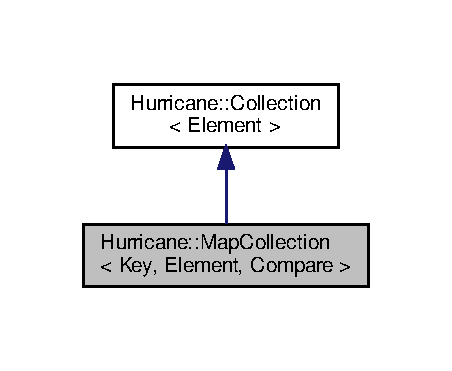
\includegraphics[width=217pt]{classHurricane_1_1MapCollection__inherit__graph}
\end{center}
\end{figure}
\doxysubsection*{Public Member Functions}
\begin{Indent}\textbf{ Collection Collection}\par
{\em \hypertarget{Collection_8h_secCollectionUtilitarians}{}\doxysubsection{Utilitarians}\label{Collection_8h_secCollectionUtilitarians}
{\bfseries{Collection\+::\+Fill}} {\bfseries{Collection\+::\+Fill}} {\bfseries{Collection\+::\+Fill}} \begin{DoxyRemark}{Remarks}
The elements are added to the container in the order with which the collection is visited. So the same order will appear in a list or a vector, but for a set they will be inserted according to the set ordering method. 
\end{DoxyRemark}
}\begin{DoxyCompactItemize}
\item 
\mbox{\hyperlink{classHurricane_1_1MapCollection_a0b905fb46ced35815132e5eab62a8de1}{Map\+Collection}} (const Element\+Map $\ast$element\+Map=NULL)
\end{DoxyCompactItemize}
\end{Indent}


\doxysubsection{Detailed Description}
\subsubsection*{template$<$class Key, class Element, class Compare = less$<$\+Key$>$$>$\newline
class Hurricane\+::\+Map\+Collection$<$ Key, Element, Compare $>$}

\mbox{\hyperlink{namespaceHurricane}{Hurricane}} \mbox{\hyperlink{classHurricane_1_1Collection}{Collection}} wrapper around a std\+::map. 

Automatically wrap a \mbox{\hyperlink{namespaceHurricane}{Hurricane}} \mbox{\hyperlink{classHurricane_1_1Collection}{Collection}} around a stl\+::map. 

\doxysubsection{Constructor \& Destructor Documentation}
\mbox{\Hypertarget{classHurricane_1_1MapCollection_a0b905fb46ced35815132e5eab62a8de1}\label{classHurricane_1_1MapCollection_a0b905fb46ced35815132e5eab62a8de1}} 
\index{Hurricane::MapCollection$<$ Key, Element, Compare $>$@{Hurricane::MapCollection$<$ Key, Element, Compare $>$}!MapCollection@{MapCollection}}
\index{MapCollection@{MapCollection}!Hurricane::MapCollection$<$ Key, Element, Compare $>$@{Hurricane::MapCollection$<$ Key, Element, Compare $>$}}
\doxysubsubsection{\texorpdfstring{MapCollection()}{MapCollection()}}
{\footnotesize\ttfamily template$<$class Key , class Element , class Compare  = less$<$\+Key$>$$>$ \\
\mbox{\hyperlink{classHurricane_1_1MapCollection}{Hurricane\+::\+Map\+Collection}}$<$ Key, Element, Compare $>$\+::\mbox{\hyperlink{classHurricane_1_1MapCollection}{Map\+Collection}} (\begin{DoxyParamCaption}\item[{const Element\+Map $\ast$}]{element\+Map = {\ttfamily NULL} }\end{DoxyParamCaption})\hspace{0.3cm}{\ttfamily [inline]}}

Constructor from a STL map, the map must not be de-\/allocated. 

The documentation for this class was generated from the following files\+:\begin{DoxyCompactItemize}
\item 
Map\+Collection.\+h\item 
Collection.\+dox\end{DoxyCompactItemize}

\hypertarget{classHurricane_1_1BasicLayer_1_1Material}{}\doxysection{Hurricane\+::Basic\+Layer\+::Material Class Reference}
\label{classHurricane_1_1BasicLayer_1_1Material}\index{Hurricane::BasicLayer::Material@{Hurricane::BasicLayer::Material}}
\doxysubsection*{Public Types}
\begin{Indent}\textbf{ Basic\+Layer Collection}\par
\begin{DoxyCompactItemize}
\item 
enum \mbox{\hyperlink{classHurricane_1_1BasicLayer_1_1Material_a3e815440ad4b86b3569fa54ca06fc3e8}{Code}} \{ \newline
\mbox{\hyperlink{classHurricane_1_1BasicLayer_1_1Material_a3e815440ad4b86b3569fa54ca06fc3e8acdf0cf84e1b081113add657e0a8bd49c}{n\+Well}} =0
, \newline
\mbox{\hyperlink{classHurricane_1_1BasicLayer_1_1Material_a3e815440ad4b86b3569fa54ca06fc3e8abab32187e9c4013a84e39cb6283bcc92}{p\+Well}}
, \newline
\mbox{\hyperlink{classHurricane_1_1BasicLayer_1_1Material_a3e815440ad4b86b3569fa54ca06fc3e8ac4e1ac9fce1c8328c415aebc024d1fda}{n\+Implant}}
, \newline
\mbox{\hyperlink{classHurricane_1_1BasicLayer_1_1Material_a3e815440ad4b86b3569fa54ca06fc3e8a73d7adbdda868d5e680a24ce3c20279e}{p\+Implant}}
, \newline
\mbox{\hyperlink{classHurricane_1_1BasicLayer_1_1Material_a3e815440ad4b86b3569fa54ca06fc3e8ab67cfb3c192135ea8d52452a8932f7b7}{active}}
, \newline
\mbox{\hyperlink{classHurricane_1_1BasicLayer_1_1Material_a3e815440ad4b86b3569fa54ca06fc3e8a506eb536d54e1005b664cc0f2c101670}{poly}}
, \newline
\mbox{\hyperlink{classHurricane_1_1BasicLayer_1_1Material_a3e815440ad4b86b3569fa54ca06fc3e8ac853c14f5754c0d802b5be0f8068b4cf}{cut}}
, \newline
\mbox{\hyperlink{classHurricane_1_1BasicLayer_1_1Material_a3e815440ad4b86b3569fa54ca06fc3e8a9f5ac52339b7bd9bbf7cdac468c51924}{metal}}
, \newline
\mbox{\hyperlink{classHurricane_1_1BasicLayer_1_1Material_a3e815440ad4b86b3569fa54ca06fc3e8a0dd9279952186054fda92b8a97b253fd}{blockage}}
, \newline
{\bfseries info}
, \newline
\mbox{\hyperlink{classHurricane_1_1BasicLayer_1_1Material_a3e815440ad4b86b3569fa54ca06fc3e8a43faff93bcb2788ccb23905cc0d07bec}{other}}
 \}
\end{DoxyCompactItemize}
\end{Indent}


\doxysubsection{Detailed Description}
Encapsulate the \mbox{\hyperlink{classHurricane_1_1BasicLayer_1_1Material_a3e815440ad4b86b3569fa54ca06fc3e8}{Basic\+Layer\+::\+Material\+::\+Code}} enumeration that defines the \mbox{\hyperlink{classHurricane_1_1BasicLayer}{Basic\+Layer}} purpose. 

\doxysubsection{Member Enumeration Documentation}
\mbox{\Hypertarget{classHurricane_1_1BasicLayer_1_1Material_a3e815440ad4b86b3569fa54ca06fc3e8}\label{classHurricane_1_1BasicLayer_1_1Material_a3e815440ad4b86b3569fa54ca06fc3e8}} 
\index{Hurricane::BasicLayer::Material@{Hurricane::BasicLayer::Material}!Code@{Code}}
\index{Code@{Code}!Hurricane::BasicLayer::Material@{Hurricane::BasicLayer::Material}}
\doxysubsubsection{\texorpdfstring{Code}{Code}}
{\footnotesize\ttfamily enum \mbox{\hyperlink{classHurricane_1_1BasicLayer_1_1Material_a3e815440ad4b86b3569fa54ca06fc3e8}{Hurricane\+::\+Basic\+Layer\+::\+Material\+::\+Code}}}

This enumeration defines the layer purpose inside the \mbox{\hyperlink{classHurricane_1_1BasicLayer_1_1Material}{Basic\+Layer\+::\+Material}}. \begin{DoxyEnumFields}{Enumerator}
\raisebox{\heightof{T}}[0pt][0pt]{\index{nWell@{nWell}!Hurricane::BasicLayer::Material@{Hurricane::BasicLayer::Material}}\index{Hurricane::BasicLayer::Material@{Hurricane::BasicLayer::Material}!nWell@{nWell}}}\mbox{\Hypertarget{classHurricane_1_1BasicLayer_1_1Material_a3e815440ad4b86b3569fa54ca06fc3e8acdf0cf84e1b081113add657e0a8bd49c}\label{classHurricane_1_1BasicLayer_1_1Material_a3e815440ad4b86b3569fa54ca06fc3e8acdf0cf84e1b081113add657e0a8bd49c}} 
n\+Well&This is a NWELL layer. \\
\hline

\raisebox{\heightof{T}}[0pt][0pt]{\index{pWell@{pWell}!Hurricane::BasicLayer::Material@{Hurricane::BasicLayer::Material}}\index{Hurricane::BasicLayer::Material@{Hurricane::BasicLayer::Material}!pWell@{pWell}}}\mbox{\Hypertarget{classHurricane_1_1BasicLayer_1_1Material_a3e815440ad4b86b3569fa54ca06fc3e8abab32187e9c4013a84e39cb6283bcc92}\label{classHurricane_1_1BasicLayer_1_1Material_a3e815440ad4b86b3569fa54ca06fc3e8abab32187e9c4013a84e39cb6283bcc92}} 
p\+Well&This is a PWELL layer. \\
\hline

\raisebox{\heightof{T}}[0pt][0pt]{\index{nImplant@{nImplant}!Hurricane::BasicLayer::Material@{Hurricane::BasicLayer::Material}}\index{Hurricane::BasicLayer::Material@{Hurricane::BasicLayer::Material}!nImplant@{nImplant}}}\mbox{\Hypertarget{classHurricane_1_1BasicLayer_1_1Material_a3e815440ad4b86b3569fa54ca06fc3e8ac4e1ac9fce1c8328c415aebc024d1fda}\label{classHurricane_1_1BasicLayer_1_1Material_a3e815440ad4b86b3569fa54ca06fc3e8ac4e1ac9fce1c8328c415aebc024d1fda}} 
n\+Implant&This is a N implant layer, for transistor source \& drain. \\
\hline

\raisebox{\heightof{T}}[0pt][0pt]{\index{pImplant@{pImplant}!Hurricane::BasicLayer::Material@{Hurricane::BasicLayer::Material}}\index{Hurricane::BasicLayer::Material@{Hurricane::BasicLayer::Material}!pImplant@{pImplant}}}\mbox{\Hypertarget{classHurricane_1_1BasicLayer_1_1Material_a3e815440ad4b86b3569fa54ca06fc3e8a73d7adbdda868d5e680a24ce3c20279e}\label{classHurricane_1_1BasicLayer_1_1Material_a3e815440ad4b86b3569fa54ca06fc3e8a73d7adbdda868d5e680a24ce3c20279e}} 
p\+Implant&This is a P implant layer, for transistor source \& drain. \\
\hline

\raisebox{\heightof{T}}[0pt][0pt]{\index{active@{active}!Hurricane::BasicLayer::Material@{Hurricane::BasicLayer::Material}}\index{Hurricane::BasicLayer::Material@{Hurricane::BasicLayer::Material}!active@{active}}}\mbox{\Hypertarget{classHurricane_1_1BasicLayer_1_1Material_a3e815440ad4b86b3569fa54ca06fc3e8ab67cfb3c192135ea8d52452a8932f7b7}\label{classHurricane_1_1BasicLayer_1_1Material_a3e815440ad4b86b3569fa54ca06fc3e8ab67cfb3c192135ea8d52452a8932f7b7}} 
active&For active area, for transistor gates. \\
\hline

\raisebox{\heightof{T}}[0pt][0pt]{\index{poly@{poly}!Hurricane::BasicLayer::Material@{Hurricane::BasicLayer::Material}}\index{Hurricane::BasicLayer::Material@{Hurricane::BasicLayer::Material}!poly@{poly}}}\mbox{\Hypertarget{classHurricane_1_1BasicLayer_1_1Material_a3e815440ad4b86b3569fa54ca06fc3e8a506eb536d54e1005b664cc0f2c101670}\label{classHurricane_1_1BasicLayer_1_1Material_a3e815440ad4b86b3569fa54ca06fc3e8a506eb536d54e1005b664cc0f2c101670}} 
poly&Polysilicium, for short connections \& transistor gates. \\
\hline

\raisebox{\heightof{T}}[0pt][0pt]{\index{cut@{cut}!Hurricane::BasicLayer::Material@{Hurricane::BasicLayer::Material}}\index{Hurricane::BasicLayer::Material@{Hurricane::BasicLayer::Material}!cut@{cut}}}\mbox{\Hypertarget{classHurricane_1_1BasicLayer_1_1Material_a3e815440ad4b86b3569fa54ca06fc3e8ac853c14f5754c0d802b5be0f8068b4cf}\label{classHurricane_1_1BasicLayer_1_1Material_a3e815440ad4b86b3569fa54ca06fc3e8ac853c14f5754c0d802b5be0f8068b4cf}} 
cut&For the {\itshape hole} part of VIAs. \\
\hline

\raisebox{\heightof{T}}[0pt][0pt]{\index{metal@{metal}!Hurricane::BasicLayer::Material@{Hurricane::BasicLayer::Material}}\index{Hurricane::BasicLayer::Material@{Hurricane::BasicLayer::Material}!metal@{metal}}}\mbox{\Hypertarget{classHurricane_1_1BasicLayer_1_1Material_a3e815440ad4b86b3569fa54ca06fc3e8a9f5ac52339b7bd9bbf7cdac468c51924}\label{classHurricane_1_1BasicLayer_1_1Material_a3e815440ad4b86b3569fa54ca06fc3e8a9f5ac52339b7bd9bbf7cdac468c51924}} 
metal&For routing layers. \\
\hline

\raisebox{\heightof{T}}[0pt][0pt]{\index{blockage@{blockage}!Hurricane::BasicLayer::Material@{Hurricane::BasicLayer::Material}}\index{Hurricane::BasicLayer::Material@{Hurricane::BasicLayer::Material}!blockage@{blockage}}}\mbox{\Hypertarget{classHurricane_1_1BasicLayer_1_1Material_a3e815440ad4b86b3569fa54ca06fc3e8a0dd9279952186054fda92b8a97b253fd}\label{classHurricane_1_1BasicLayer_1_1Material_a3e815440ad4b86b3569fa54ca06fc3e8a0dd9279952186054fda92b8a97b253fd}} 
blockage&For blockages, associated to metals. \\
\hline

\raisebox{\heightof{T}}[0pt][0pt]{\index{other@{other}!Hurricane::BasicLayer::Material@{Hurricane::BasicLayer::Material}}\index{Hurricane::BasicLayer::Material@{Hurricane::BasicLayer::Material}!other@{other}}}\mbox{\Hypertarget{classHurricane_1_1BasicLayer_1_1Material_a3e815440ad4b86b3569fa54ca06fc3e8a43faff93bcb2788ccb23905cc0d07bec}\label{classHurricane_1_1BasicLayer_1_1Material_a3e815440ad4b86b3569fa54ca06fc3e8a43faff93bcb2788ccb23905cc0d07bec}} 
other&Fallback for any other purposes. \\
\hline

\end{DoxyEnumFields}


The documentation for this class was generated from the following files\+:\begin{DoxyCompactItemize}
\item 
Basic\+Layer.\+h\item 
Basic\+Layer.\+dox\end{DoxyCompactItemize}

\hypertarget{classHurricane_1_1Name}{}\doxysection{Hurricane\+::Name Class Reference}
\label{classHurricane_1_1Name}\index{Hurricane::Name@{Hurricane::Name}}


\mbox{\hyperlink{classHurricane_1_1Name}{Name}} description ({\bfseries{API}})  


\doxysubsection*{Public Member Functions}
\begin{DoxyCompactItemize}
\item 
\mbox{\hyperlink{classHurricane_1_1Name_a42636ecb0d4d7d03eb881420a244038b}{Name}} ()
\item 
\mbox{\hyperlink{classHurricane_1_1Name_a754d54199d54c5e4568421c89f0682cb}{Name}} (const char $\ast$c)
\item 
\mbox{\hyperlink{classHurricane_1_1Name_a446df795ebe2e641710696bf775eb491}{Name}} (const string \&s)
\item 
\mbox{\hyperlink{classHurricane_1_1Name_a56ffee3e75dc343c7ec8b61102c1d3a2}{Name}} (const \mbox{\hyperlink{classHurricane_1_1Name}{Name}} \&name)
\item 
\mbox{\hyperlink{classHurricane_1_1Name_a1ce605ce16980334f93d7cc278984842}{$\sim$\+Name}} ()
\item 
\mbox{\hyperlink{classHurricane_1_1Name}{Name}} \& \mbox{\hyperlink{classHurricane_1_1Name_adcd165de286782c011acc31727adb4a1}{operator=}} (const \mbox{\hyperlink{classHurricane_1_1Name}{Name}} \&name)
\item 
bool \mbox{\hyperlink{classHurricane_1_1Name_a3b728f0b8aa027639ebd47c60addf738}{operator==}} (const \mbox{\hyperlink{classHurricane_1_1Name}{Name}} \&name) const
\item 
bool \mbox{\hyperlink{classHurricane_1_1Name_aff97f0bcf698ad76f6f3c9a4c4833cc3}{operator!=}} (const \mbox{\hyperlink{classHurricane_1_1Name}{Name}} \&name) const
\item 
bool \mbox{\hyperlink{classHurricane_1_1Name_a9ce91a54cd340fb1e14baf56797f1577}{operator$<$}} (const \mbox{\hyperlink{classHurricane_1_1Name}{Name}} \&name) const
\item 
bool \mbox{\hyperlink{classHurricane_1_1Name_a9704f9fe4c605a86de13b6a8d90feab2}{operator$<$=}} (const \mbox{\hyperlink{classHurricane_1_1Name}{Name}} \&name) const
\item 
bool \mbox{\hyperlink{classHurricane_1_1Name_a33bd981f4f6923a50c603cd06283032d}{operator$>$}} (const \mbox{\hyperlink{classHurricane_1_1Name}{Name}} \&name) const
\item 
bool \mbox{\hyperlink{classHurricane_1_1Name_a241d0568f16c8ba60d4c5148be6a48b3}{operator$>$=}} (const \mbox{\hyperlink{classHurricane_1_1Name}{Name}} \&name) const
\item 
char \mbox{\hyperlink{classHurricane_1_1Name_a2e6f3869321016de8f98f2b35f136ab4}{operator\mbox{[}$\,$\mbox{]}}} (unsigned index) const
\item 
bool \mbox{\hyperlink{classHurricane_1_1Name_a6c05cf200a0aeb95f98603fa0c9c9d4b}{is\+Empty}} () const
\end{DoxyCompactItemize}


\doxysubsection{Detailed Description}
\mbox{\hyperlink{classHurricane_1_1Name}{Name}} description ({\bfseries{API}}) 

\hypertarget{classHurricane_1_1Name_secNameIntro}{}\doxysubsection{Introduction}\label{classHurricane_1_1Name_secNameIntro}
Those objects provide an automatic management of shared name (character strings).

The underlying representation is based on a string shared by the different names. Each shared string is automatically released when the last name referencing it disapears (managed by a reference count technic). 

\doxysubsection{Constructor \& Destructor Documentation}
\mbox{\Hypertarget{classHurricane_1_1Name_a42636ecb0d4d7d03eb881420a244038b}\label{classHurricane_1_1Name_a42636ecb0d4d7d03eb881420a244038b}} 
\index{Hurricane::Name@{Hurricane::Name}!Name@{Name}}
\index{Name@{Name}!Hurricane::Name@{Hurricane::Name}}
\doxysubsubsection{\texorpdfstring{Name()}{Name()}\hspace{0.1cm}{\footnotesize\ttfamily [1/4]}}
{\footnotesize\ttfamily Hurricane\+::\+Name\+::\+Name (\begin{DoxyParamCaption}{ }\end{DoxyParamCaption})}

Default constructor (initialized with an empty string). \mbox{\Hypertarget{classHurricane_1_1Name_a754d54199d54c5e4568421c89f0682cb}\label{classHurricane_1_1Name_a754d54199d54c5e4568421c89f0682cb}} 
\index{Hurricane::Name@{Hurricane::Name}!Name@{Name}}
\index{Name@{Name}!Hurricane::Name@{Hurricane::Name}}
\doxysubsubsection{\texorpdfstring{Name()}{Name()}\hspace{0.1cm}{\footnotesize\ttfamily [2/4]}}
{\footnotesize\ttfamily Hurricane\+::\+Name\+::\+Name (\begin{DoxyParamCaption}\item[{const char $\ast$}]{s }\end{DoxyParamCaption})}

Standard constructor, from a C like character string. \mbox{\Hypertarget{classHurricane_1_1Name_a446df795ebe2e641710696bf775eb491}\label{classHurricane_1_1Name_a446df795ebe2e641710696bf775eb491}} 
\index{Hurricane::Name@{Hurricane::Name}!Name@{Name}}
\index{Name@{Name}!Hurricane::Name@{Hurricane::Name}}
\doxysubsubsection{\texorpdfstring{Name()}{Name()}\hspace{0.1cm}{\footnotesize\ttfamily [3/4]}}
{\footnotesize\ttfamily Hurricane\+::\+Name\+::\+Name (\begin{DoxyParamCaption}\item[{const string \&}]{s }\end{DoxyParamCaption})}

Standard constructor, from a STL string. \mbox{\Hypertarget{classHurricane_1_1Name_a56ffee3e75dc343c7ec8b61102c1d3a2}\label{classHurricane_1_1Name_a56ffee3e75dc343c7ec8b61102c1d3a2}} 
\index{Hurricane::Name@{Hurricane::Name}!Name@{Name}}
\index{Name@{Name}!Hurricane::Name@{Hurricane::Name}}
\doxysubsubsection{\texorpdfstring{Name()}{Name()}\hspace{0.1cm}{\footnotesize\ttfamily [4/4]}}
{\footnotesize\ttfamily Hurricane\+::\+Name\+::\+Name (\begin{DoxyParamCaption}\item[{const \mbox{\hyperlink{classHurricane_1_1Name}{Name}} \&}]{name }\end{DoxyParamCaption})}

Copy constructor. \mbox{\Hypertarget{classHurricane_1_1Name_a1ce605ce16980334f93d7cc278984842}\label{classHurricane_1_1Name_a1ce605ce16980334f93d7cc278984842}} 
\index{Hurricane::Name@{Hurricane::Name}!````~Name@{$\sim$Name}}
\index{````~Name@{$\sim$Name}!Hurricane::Name@{Hurricane::Name}}
\doxysubsubsection{\texorpdfstring{$\sim$Name()}{~Name()}}
{\footnotesize\ttfamily Hurricane\+::\+Name\+::$\sim$\+Name (\begin{DoxyParamCaption}{ }\end{DoxyParamCaption})}

The destructor releases the shared string if it no longer referenced. 

\doxysubsection{Member Function Documentation}
\mbox{\Hypertarget{classHurricane_1_1Name_adcd165de286782c011acc31727adb4a1}\label{classHurricane_1_1Name_adcd165de286782c011acc31727adb4a1}} 
\index{Hurricane::Name@{Hurricane::Name}!operator=@{operator=}}
\index{operator=@{operator=}!Hurricane::Name@{Hurricane::Name}}
\doxysubsubsection{\texorpdfstring{operator=()}{operator=()}}
{\footnotesize\ttfamily \mbox{\hyperlink{classHurricane_1_1Name}{Name}} \& Hurricane\+::\+Name\+::operator= (\begin{DoxyParamCaption}\item[{const \mbox{\hyperlink{classHurricane_1_1Name}{Name}} \&}]{name }\end{DoxyParamCaption})}

Assignment operator. Very fast because there is only an assignement of pointer to the shared string and an incrementation of its reference counter. \mbox{\Hypertarget{classHurricane_1_1Name_a3b728f0b8aa027639ebd47c60addf738}\label{classHurricane_1_1Name_a3b728f0b8aa027639ebd47c60addf738}} 
\index{Hurricane::Name@{Hurricane::Name}!operator==@{operator==}}
\index{operator==@{operator==}!Hurricane::Name@{Hurricane::Name}}
\doxysubsubsection{\texorpdfstring{operator==()}{operator==()}}
{\footnotesize\ttfamily bool Hurricane\+::\+Name\+::operator== (\begin{DoxyParamCaption}\item[{const \mbox{\hyperlink{classHurricane_1_1Name}{Name}} \&}]{name }\end{DoxyParamCaption}) const}

Equality operator. Very fast because it only tests the equality of pointers to the two shared strings (and not the equality of the two strings).

\begin{DoxyRemark}{Remarks}
Don\textquotesingle{}t loose on one side what you save on the other as shown in the following code \+: 
\begin{DoxyCode}{0}
\DoxyCodeLine{Cell* cell = ...; \textcolor{comment}{// we get the cell}}
\DoxyCodeLine{ }
\DoxyCodeLine{for\_each\_net(net, cellGetNets()) \{}
\DoxyCodeLine{   \textcolor{keywordflow}{if} (netGetName() == \textcolor{stringliteral}{"{}vdd"{}}) \{}
\DoxyCodeLine{      ... ;}
\DoxyCodeLine{   \}}
\DoxyCodeLine{   end\_for;}
\DoxyCodeLine{\}}

\end{DoxyCode}
 Indeed, for each equality test, a name will be created from the string \char`\"{}vdd\char`\"{}. If the equality test is very fast, it is not the same for the name construction. So it is faster to write \+: 
\begin{DoxyCode}{0}
\DoxyCodeLine{Cell* cell = ...; \textcolor{comment}{// we get the cell}}
\DoxyCodeLine{ }
\DoxyCodeLine{\mbox{\hyperlink{classHurricane_1_1Name_a42636ecb0d4d7d03eb881420a244038b}{Name}} vdd = \textcolor{stringliteral}{"{}vdd"{}};}
\DoxyCodeLine{for\_each\_net(net, cellGetNets()) \{}
\DoxyCodeLine{   \textcolor{keywordflow}{if} (netGetName() == vdd) \{}
\DoxyCodeLine{      ...}
\DoxyCodeLine{   \}}
\DoxyCodeLine{   end\_for;}
\DoxyCodeLine{\}}

\end{DoxyCode}
 Or yet faster \+: 
\begin{DoxyCode}{0}
\DoxyCodeLine{Cell* cell = ...; \textcolor{comment}{// we get the cell}}
\DoxyCodeLine{ }
\DoxyCodeLine{\textcolor{keyword}{static} \mbox{\hyperlink{classHurricane_1_1Name_a42636ecb0d4d7d03eb881420a244038b}{Name}} VDD = \textcolor{stringliteral}{"{}vdd"{}};}
\DoxyCodeLine{for\_each\_net(net, cellGetNets()) \{}
\DoxyCodeLine{   \textcolor{keywordflow}{if} (netGetName() == VDD) \{}
\DoxyCodeLine{      ...}
\DoxyCodeLine{   \}}
\DoxyCodeLine{   end\_for;}
\DoxyCodeLine{\}}

\end{DoxyCode}
 
\end{DoxyRemark}
\mbox{\Hypertarget{classHurricane_1_1Name_aff97f0bcf698ad76f6f3c9a4c4833cc3}\label{classHurricane_1_1Name_aff97f0bcf698ad76f6f3c9a4c4833cc3}} 
\index{Hurricane::Name@{Hurricane::Name}!operator"!=@{operator"!=}}
\index{operator"!=@{operator"!=}!Hurricane::Name@{Hurricane::Name}}
\doxysubsubsection{\texorpdfstring{operator"!=()}{operator!=()}}
{\footnotesize\ttfamily bool Hurricane\+::\+Name\+::operator!= (\begin{DoxyParamCaption}\item[{const \mbox{\hyperlink{classHurricane_1_1Name}{Name}} \&}]{name }\end{DoxyParamCaption}) const}

Difference operator. Very fast because it only tests the difference of pointers to the two shared strings (and not the difference of the two strings). \mbox{\Hypertarget{classHurricane_1_1Name_a9ce91a54cd340fb1e14baf56797f1577}\label{classHurricane_1_1Name_a9ce91a54cd340fb1e14baf56797f1577}} 
\index{Hurricane::Name@{Hurricane::Name}!operator$<$@{operator$<$}}
\index{operator$<$@{operator$<$}!Hurricane::Name@{Hurricane::Name}}
\doxysubsubsection{\texorpdfstring{operator$<$()}{operator<()}}
{\footnotesize\ttfamily bool Hurricane\+::\+Name\+::operator$<$ (\begin{DoxyParamCaption}\item[{const \mbox{\hyperlink{classHurricane_1_1Name}{Name}} \&}]{name }\end{DoxyParamCaption}) const}

No description. \mbox{\Hypertarget{classHurricane_1_1Name_a9704f9fe4c605a86de13b6a8d90feab2}\label{classHurricane_1_1Name_a9704f9fe4c605a86de13b6a8d90feab2}} 
\index{Hurricane::Name@{Hurricane::Name}!operator$<$=@{operator$<$=}}
\index{operator$<$=@{operator$<$=}!Hurricane::Name@{Hurricane::Name}}
\doxysubsubsection{\texorpdfstring{operator$<$=()}{operator<=()}}
{\footnotesize\ttfamily bool Hurricane\+::\+Name\+::operator$<$= (\begin{DoxyParamCaption}\item[{const \mbox{\hyperlink{classHurricane_1_1Name}{Name}} \&}]{name }\end{DoxyParamCaption}) const}

No description. \mbox{\Hypertarget{classHurricane_1_1Name_a33bd981f4f6923a50c603cd06283032d}\label{classHurricane_1_1Name_a33bd981f4f6923a50c603cd06283032d}} 
\index{Hurricane::Name@{Hurricane::Name}!operator$>$@{operator$>$}}
\index{operator$>$@{operator$>$}!Hurricane::Name@{Hurricane::Name}}
\doxysubsubsection{\texorpdfstring{operator$>$()}{operator>()}}
{\footnotesize\ttfamily bool Hurricane\+::\+Name\+::operator$>$ (\begin{DoxyParamCaption}\item[{const \mbox{\hyperlink{classHurricane_1_1Name}{Name}} \&}]{name }\end{DoxyParamCaption}) const}

No description. \mbox{\Hypertarget{classHurricane_1_1Name_a241d0568f16c8ba60d4c5148be6a48b3}\label{classHurricane_1_1Name_a241d0568f16c8ba60d4c5148be6a48b3}} 
\index{Hurricane::Name@{Hurricane::Name}!operator$>$=@{operator$>$=}}
\index{operator$>$=@{operator$>$=}!Hurricane::Name@{Hurricane::Name}}
\doxysubsubsection{\texorpdfstring{operator$>$=()}{operator>=()}}
{\footnotesize\ttfamily bool Hurricane\+::\+Name\+::operator$>$= (\begin{DoxyParamCaption}\item[{const \mbox{\hyperlink{classHurricane_1_1Name}{Name}} \&}]{name }\end{DoxyParamCaption}) const}

Those operators need to process the two shared strings and are not as fast as the previous ones. \mbox{\Hypertarget{classHurricane_1_1Name_a2e6f3869321016de8f98f2b35f136ab4}\label{classHurricane_1_1Name_a2e6f3869321016de8f98f2b35f136ab4}} 
\index{Hurricane::Name@{Hurricane::Name}!operator\mbox{[}\mbox{]}@{operator[]}}
\index{operator\mbox{[}\mbox{]}@{operator[]}!Hurricane::Name@{Hurricane::Name}}
\doxysubsubsection{\texorpdfstring{operator[]()}{operator[]()}}
{\footnotesize\ttfamily char Hurricane\+::\+Name\+::operator\mbox{[}$\,$\mbox{]} (\begin{DoxyParamCaption}\item[{unsigned}]{index }\end{DoxyParamCaption}) const}

Indexation operator (for reading the character of rank index). Throws an exception if index is out of bounds. \mbox{\Hypertarget{classHurricane_1_1Name_a6c05cf200a0aeb95f98603fa0c9c9d4b}\label{classHurricane_1_1Name_a6c05cf200a0aeb95f98603fa0c9c9d4b}} 
\index{Hurricane::Name@{Hurricane::Name}!isEmpty@{isEmpty}}
\index{isEmpty@{isEmpty}!Hurricane::Name@{Hurricane::Name}}
\doxysubsubsection{\texorpdfstring{isEmpty()}{isEmpty()}}
{\footnotesize\ttfamily bool Hurricane\+::\+Name\+::is\+Empty (\begin{DoxyParamCaption}{ }\end{DoxyParamCaption}) const}

{\bfseries{Returns\+:}} {\bfseries{true}} if the shared string is empty, else {\bfseries{false}}. 

The documentation for this class was generated from the following files\+:\begin{DoxyCompactItemize}
\item 
Name.\+h\item 
Name.\+dox\end{DoxyCompactItemize}

\hypertarget{classHurricane_1_1Net}{}\doxysection{Hurricane\+::Net Class Reference}
\label{classHurricane_1_1Net}\index{Hurricane::Net@{Hurricane::Net}}


\mbox{\hyperlink{classHurricane_1_1Net}{Net}} description ({\bfseries{API}})  




Inheritance diagram for Hurricane\+::Net\+:\nopagebreak
\begin{figure}[H]
\begin{center}
\leavevmode
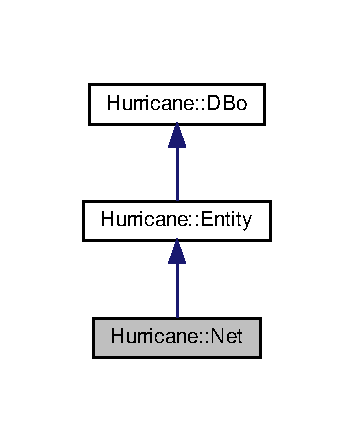
\includegraphics[width=170pt]{classHurricane_1_1Net__inherit__graph}
\end{center}
\end{figure}
\doxysubsection*{Classes}
\begin{DoxyCompactItemize}
\item 
class \mbox{\hyperlink{classHurricane_1_1Net_1_1Direction}{Direction}}
\item 
class \mbox{\hyperlink{classHurricane_1_1Net_1_1Type}{Type}}
\end{DoxyCompactItemize}
\doxysubsection*{Public Types}
\begin{DoxyCompactItemize}
\item 
typedef \mbox{\hyperlink{classHurricane_1_1Entity}{Entity}} \mbox{\hyperlink{classHurricane_1_1Net_a3f1ac0fcb03638b2ffa9af6a9a58de15}{Inherit}}
\item 
typedef unsigned \mbox{\hyperlink{classHurricane_1_1Net_a3a242d929e0c733f90f3f69be8cc427b}{Arity}}
\end{DoxyCompactItemize}
\doxysubsection*{Public Member Functions}
\begin{DoxyCompactItemize}
\item 
const \mbox{\hyperlink{classHurricane_1_1Name}{Name}} \& \mbox{\hyperlink{classHurricane_1_1Net_aeba73ca641db371dde29baf348b58bba}{get\+Name}} () const
\item 
const \mbox{\hyperlink{classHurricane_1_1Net_a3a242d929e0c733f90f3f69be8cc427b}{Arity}} \& \mbox{\hyperlink{classHurricane_1_1Net_a78de2202fcf4f16024b4460ebb7dc907}{get\+Arity}} () const
\item 
const \mbox{\hyperlink{classHurricane_1_1Net_1_1Type}{Type}} \& \mbox{\hyperlink{classHurricane_1_1Net_a0fa61dc0ccb67f384f03b35f83d391e7}{get\+Type}} () const
\item 
const \mbox{\hyperlink{classHurricane_1_1Net_1_1Direction}{Direction}} \& \mbox{\hyperlink{classHurricane_1_1Net_aa84245d734dfaa572660a1a2c1bfc56e}{get\+Direction}} () const
\item 
const \mbox{\hyperlink{classHurricane_1_1Point}{Point}} \& \mbox{\hyperlink{classHurricane_1_1Net_abcfdec9c953d228845fdb9d75e8173cc}{get\+Position}} () const
\item 
const \mbox{\hyperlink{classHurricane_1_1DbU_a4fbfa3e8c89347af76c9628ea06c4146}{Db\+U\+::\+Unit}} \& \mbox{\hyperlink{classHurricane_1_1Net_a1f8f4c4632614b84a1227a1da8310428}{getX}} () const
\item 
const \mbox{\hyperlink{classHurricane_1_1DbU_a4fbfa3e8c89347af76c9628ea06c4146}{Db\+U\+::\+Unit}} \& \mbox{\hyperlink{classHurricane_1_1Net_aa97899b408aa47ec22792b5c6d6e9216}{getY}} () const
\item 
\mbox{\hyperlink{namespaceHurricane_a7d26d99aeb5dd6d70d51bd35d2473e72}{Components}} \mbox{\hyperlink{classHurricane_1_1Net_a1e2d7ef9bab15694870a605e514f26e8}{get\+Components}} () const
\item 
\mbox{\hyperlink{namespaceHurricane_af8923abd57508cc44931a00d61b564ad}{Rubbers}} \mbox{\hyperlink{classHurricane_1_1Net_a6ddbe2697a7fd7a7cd359f97b2ad0223}{get\+Rubbers}} () const
\item 
Routing\+Pads \mbox{\hyperlink{classHurricane_1_1Net_a1078d55acf3efa0b3c23cd345cae87fa}{get\+Routing\+Pads}} () const
\item 
\mbox{\hyperlink{namespaceHurricane_ac8335d2057483ee7a935c15a9460c64f}{Plugs}} \mbox{\hyperlink{classHurricane_1_1Net_a88322672c105405a61a78022359178aa}{get\+Plugs}} () const
\item 
\mbox{\hyperlink{namespaceHurricane_a1e6a8ab09f688509bd727b3fee02d0d2}{Contacts}} \mbox{\hyperlink{classHurricane_1_1Net_a9c397596fe9ecbf674712c72e0b9010c}{get\+Contacts}} () const
\item 
\mbox{\hyperlink{namespaceHurricane_a30748fa53a81cb597d4a13d651238716}{Segments}} \mbox{\hyperlink{classHurricane_1_1Net_aadc5a9ef26d7a72f49fdf22452f3cc58}{get\+Segments}} () const
\item 
\mbox{\hyperlink{namespaceHurricane_a146e2d3d34b4035aff422f12e85345b9}{Verticals}} \mbox{\hyperlink{classHurricane_1_1Net_a97f32cf738af9cf107833ca81fe95db8}{get\+Verticals}} () const
\item 
\mbox{\hyperlink{namespaceHurricane_a721e644c7d97f2f66049ab062140b855}{Horizontals}} \mbox{\hyperlink{classHurricane_1_1Net_ad8553af888909e1c127e12e68bd000fb}{get\+Horizontals}} () const
\item 
\mbox{\hyperlink{namespaceHurricane_abd1f433c44d8b515e1b8a8810aea1610}{Pads}} \mbox{\hyperlink{classHurricane_1_1Net_a564df07be5589bc72dd6eb944855aa2b}{get\+Pads}} () const
\item 
\mbox{\hyperlink{namespaceHurricane_ac8335d2057483ee7a935c15a9460c64f}{Plugs}} \mbox{\hyperlink{classHurricane_1_1Net_a9c835d2f071155521700921d816ac1fa}{get\+Slave\+Plugs}} () const
\item 
\mbox{\hyperlink{namespaceHurricane_ac8335d2057483ee7a935c15a9460c64f}{Plugs}} \mbox{\hyperlink{classHurricane_1_1Net_a08560ffa6b0f5ecc442bf232486dd8ff}{get\+Connected\+Slave\+Plugs}} () const
\item 
\mbox{\hyperlink{namespaceHurricane_ac8335d2057483ee7a935c15a9460c64f}{Plugs}} \mbox{\hyperlink{classHurricane_1_1Net_aad3f3ea88bdea914cab3f38bdcdb843d}{get\+Unconnected\+Slave\+Plugs}} () const
\item 
bool \mbox{\hyperlink{classHurricane_1_1Net_a332e9b311809f75fc0fa3a5f36acebcc}{is\+Global}} () const
\item 
bool \mbox{\hyperlink{classHurricane_1_1Net_aeeb3735dd7451bc0054dd68ac21aae47}{is\+External}} () const
\item 
bool \mbox{\hyperlink{classHurricane_1_1Net_a9caf25bfa84478157d206979dd521ed4}{is\+Logical}} () const
\item 
bool \mbox{\hyperlink{classHurricane_1_1Net_a8807cc000bbbe1c340c71fcbfbb8fe33}{is\+Clock}} () const
\item 
bool \mbox{\hyperlink{classHurricane_1_1Net_ab8947fc6c5093341958b94148407c2a2}{is\+Supply}} () const
\item 
void \mbox{\hyperlink{classHurricane_1_1Net_a1a39702b9f4d26ba29ad0dafcdddf840}{set\+Name}} (\mbox{\hyperlink{classHurricane_1_1Name}{Name}} name)
\item 
void \mbox{\hyperlink{classHurricane_1_1Net_af5dfdca4401902ee7e1e46a1a486da38}{set\+Arity}} (const \mbox{\hyperlink{classHurricane_1_1Net_a3a242d929e0c733f90f3f69be8cc427b}{Arity}} \&arity)
\item 
void \mbox{\hyperlink{classHurricane_1_1Net_a35c84afd9dade0cb715602bcf8ec8865}{set\+Global}} (bool \mbox{\hyperlink{classHurricane_1_1Net_a332e9b311809f75fc0fa3a5f36acebcc}{is\+Global}})
\item 
void \mbox{\hyperlink{classHurricane_1_1Net_a6a30bc8282ce7e4b936e73a11549fedf}{set\+External}} (bool \mbox{\hyperlink{classHurricane_1_1Net_aeeb3735dd7451bc0054dd68ac21aae47}{is\+External}})
\item 
void \mbox{\hyperlink{classHurricane_1_1Net_a83f5ce12291b0ec5ab584d515dd8963c}{set\+Type}} (const \mbox{\hyperlink{classHurricane_1_1Net_1_1Type}{Type}} \&type)
\item 
void \mbox{\hyperlink{classHurricane_1_1Net_ac33d13bb0ddc60f369d5bfcffc4bb0f8}{set\+Direction}} (const \mbox{\hyperlink{classHurricane_1_1Net_1_1Direction}{Direction}} \&direction)
\item 
void \mbox{\hyperlink{classHurricane_1_1Net_a0a3a3232a74ebced14b14029c5199561}{set\+Position}} (const \mbox{\hyperlink{classHurricane_1_1Point}{Point}} \&position)
\item 
void \mbox{\hyperlink{classHurricane_1_1Net_ae46f7e4a9b00b265c06cb6e0ee00b806}{materialize}} ()
\item 
void \mbox{\hyperlink{classHurricane_1_1Net_a9e53a3d54b61f7081263e6d7b4fa81b9}{unmaterialize}} ()
\item 
void \mbox{\hyperlink{classHurricane_1_1Net_a442f62d23364805f39816cd543284886}{merge}} (\mbox{\hyperlink{classHurricane_1_1Net}{Net}} $\ast$net)
\item 
\mbox{\hyperlink{classHurricane_1_1Net}{Net}} $\ast$ \mbox{\hyperlink{classHurricane_1_1Net_a4bd27e6ae22606463491c28437c4068f}{get\+Clone}} (\mbox{\hyperlink{classHurricane_1_1Cell}{Cell}} $\ast$clone\+Cell)
\end{DoxyCompactItemize}
\doxysubsection*{Static Public Member Functions}
\begin{DoxyCompactItemize}
\item 
static \mbox{\hyperlink{classHurricane_1_1Net}{Net}} $\ast$ \mbox{\hyperlink{classHurricane_1_1Net_ac1524cea15e8eacbf992c0cfb9e481db}{create}} (\mbox{\hyperlink{classHurricane_1_1Cell}{Cell}} $\ast$cell, const \mbox{\hyperlink{classHurricane_1_1Name}{Name}} \&name)
\end{DoxyCompactItemize}
\begin{Indent}\textbf{ Net Collection}\par
\begin{DoxyCompactItemize}
\item 
static \mbox{\hyperlink{namespaceHurricane_a0dfd2c5b40325a919d139091312732e9}{Net\+Filter}} \mbox{\hyperlink{classHurricane_1_1Net_a1730ed1247cd9bce7fcf519ea60dc738}{get\+Is\+Global\+Filter}} ()
\item 
static \mbox{\hyperlink{namespaceHurricane_a0dfd2c5b40325a919d139091312732e9}{Net\+Filter}} \mbox{\hyperlink{classHurricane_1_1Net_a3af91a80e219e37e70229e61dfd385da}{get\+Is\+External\+Filter}} ()
\item 
static \mbox{\hyperlink{namespaceHurricane_a0dfd2c5b40325a919d139091312732e9}{Net\+Filter}} \mbox{\hyperlink{classHurricane_1_1Net_a7a2d1c4ab84bf81a16e24557d2342ea5}{get\+Is\+Internal\+Filter}} ()
\item 
static \mbox{\hyperlink{namespaceHurricane_a0dfd2c5b40325a919d139091312732e9}{Net\+Filter}} \mbox{\hyperlink{classHurricane_1_1Net_afdb2269f3a88923c25264f6f785372a1}{get\+Is\+Clock\+Filter}} ()
\item 
static \mbox{\hyperlink{namespaceHurricane_a0dfd2c5b40325a919d139091312732e9}{Net\+Filter}} \mbox{\hyperlink{classHurricane_1_1Net_ac241f44abf1f332004dd6103ee1dfa48}{get\+Is\+Supply\+Filter}} ()
\end{DoxyCompactItemize}
\end{Indent}


\doxysubsection{Detailed Description}
\mbox{\hyperlink{classHurricane_1_1Net}{Net}} description ({\bfseries{API}}) 

\hypertarget{classHurricane_1_1Net_secNetPredefinedFilters}{}\doxysubsection{Predefined filters}\label{classHurricane_1_1Net_secNetPredefinedFilters}

\begin{DoxyItemize}
\item {\bfseries{\mbox{\hyperlink{classHurricane_1_1Net_a1730ed1247cd9bce7fcf519ea60dc738}{Hurricane\+::\+Net\+::get\+Is\+Global\+Filter}}}}
\item {\bfseries{\mbox{\hyperlink{classHurricane_1_1Net_a3af91a80e219e37e70229e61dfd385da}{Hurricane\+::\+Net\+::get\+Is\+External\+Filter}}}}
\item {\bfseries{\mbox{\hyperlink{classHurricane_1_1Net_a7a2d1c4ab84bf81a16e24557d2342ea5}{Hurricane\+::\+Net\+::get\+Is\+Internal\+Filter}}}}
\item {\bfseries{\mbox{\hyperlink{classHurricane_1_1Net_afdb2269f3a88923c25264f6f785372a1}{Hurricane\+::\+Net\+::get\+Is\+Clock\+Filter}}}}
\item {\bfseries{\mbox{\hyperlink{classHurricane_1_1Net_ac241f44abf1f332004dd6103ee1dfa48}{Hurricane\+::\+Net\+::get\+Is\+Supply\+Filter}}}} 
\end{DoxyItemize}

\doxysubsection{Member Typedef Documentation}
\mbox{\Hypertarget{classHurricane_1_1Net_a3f1ac0fcb03638b2ffa9af6a9a58de15}\label{classHurricane_1_1Net_a3f1ac0fcb03638b2ffa9af6a9a58de15}} 
\index{Hurricane::Net@{Hurricane::Net}!Inherit@{Inherit}}
\index{Inherit@{Inherit}!Hurricane::Net@{Hurricane::Net}}
\doxysubsubsection{\texorpdfstring{Inherit}{Inherit}}
{\footnotesize\ttfamily \mbox{\hyperlink{classHurricane_1_1Net_a3f1ac0fcb03638b2ffa9af6a9a58de15}{Hurricane\+::\+Net\+::\+Inherit}}}

Useful for calling upon methods of the base class without knowing it. \mbox{\Hypertarget{classHurricane_1_1Net_a3a242d929e0c733f90f3f69be8cc427b}\label{classHurricane_1_1Net_a3a242d929e0c733f90f3f69be8cc427b}} 
\index{Hurricane::Net@{Hurricane::Net}!Arity@{Arity}}
\index{Arity@{Arity}!Hurricane::Net@{Hurricane::Net}}
\doxysubsubsection{\texorpdfstring{Arity}{Arity}}
{\footnotesize\ttfamily \mbox{\hyperlink{classHurricane_1_1Net_a3a242d929e0c733f90f3f69be8cc427b}{Hurricane\+::\+Net\+::\+Arity}}}

This type allows to represent the number of bits associated to a net (a null value meaning undefined). 

\doxysubsection{Member Function Documentation}
\mbox{\Hypertarget{classHurricane_1_1Net_ac1524cea15e8eacbf992c0cfb9e481db}\label{classHurricane_1_1Net_ac1524cea15e8eacbf992c0cfb9e481db}} 
\index{Hurricane::Net@{Hurricane::Net}!create@{create}}
\index{create@{create}!Hurricane::Net@{Hurricane::Net}}
\doxysubsubsection{\texorpdfstring{create()}{create()}}
{\footnotesize\ttfamily \mbox{\hyperlink{classHurricane_1_1Net}{Net}} $\ast$ Hurricane\+::\+Net\+::create (\begin{DoxyParamCaption}\item[{\mbox{\hyperlink{classHurricane_1_1Cell}{Cell}} $\ast$}]{cell,  }\item[{const \mbox{\hyperlink{classHurricane_1_1Name}{Name}} \&}]{name }\end{DoxyParamCaption})\hspace{0.3cm}{\ttfamily [static]}}

Creates and returns a new net named {\ttfamily $<$name$>$} for the cell {\ttfamily $<$cell$>$}.

\begin{DoxyParagraph}{Caution\+: Throws an exception if the cell is null, if the name empty or }
if a net with same name already exists. 
\end{DoxyParagraph}
\mbox{\Hypertarget{classHurricane_1_1Net_aeba73ca641db371dde29baf348b58bba}\label{classHurricane_1_1Net_aeba73ca641db371dde29baf348b58bba}} 
\index{Hurricane::Net@{Hurricane::Net}!getName@{getName}}
\index{getName@{getName}!Hurricane::Net@{Hurricane::Net}}
\doxysubsubsection{\texorpdfstring{getName()}{getName()}}
{\footnotesize\ttfamily const \mbox{\hyperlink{classHurricane_1_1Name}{Name}} \& Hurricane\+::\+Net\+::get\+Name (\begin{DoxyParamCaption}{ }\end{DoxyParamCaption}) const\hspace{0.3cm}{\ttfamily [inline]}}

{\bfseries{Returns\+:}} the net name. \mbox{\Hypertarget{classHurricane_1_1Net_a78de2202fcf4f16024b4460ebb7dc907}\label{classHurricane_1_1Net_a78de2202fcf4f16024b4460ebb7dc907}} 
\index{Hurricane::Net@{Hurricane::Net}!getArity@{getArity}}
\index{getArity@{getArity}!Hurricane::Net@{Hurricane::Net}}
\doxysubsubsection{\texorpdfstring{getArity()}{getArity()}}
{\footnotesize\ttfamily const \mbox{\hyperlink{classHurricane_1_1Net_a3a242d929e0c733f90f3f69be8cc427b}{Net\+::\+Arity}} \& Hurricane\+::\+Net\+::get\+Arity (\begin{DoxyParamCaption}{ }\end{DoxyParamCaption}) const\hspace{0.3cm}{\ttfamily [inline]}}

{\bfseries{Returns\+:}} the signal arity (by default set to 1). \mbox{\Hypertarget{classHurricane_1_1Net_a0fa61dc0ccb67f384f03b35f83d391e7}\label{classHurricane_1_1Net_a0fa61dc0ccb67f384f03b35f83d391e7}} 
\index{Hurricane::Net@{Hurricane::Net}!getType@{getType}}
\index{getType@{getType}!Hurricane::Net@{Hurricane::Net}}
\doxysubsubsection{\texorpdfstring{getType()}{getType()}}
{\footnotesize\ttfamily const \mbox{\hyperlink{classHurricane_1_1Net_1_1Type}{Net\+::\+Type}} \& Hurricane\+::\+Net\+::get\+Type (\begin{DoxyParamCaption}{ }\end{DoxyParamCaption}) const\hspace{0.3cm}{\ttfamily [inline]}}

{\bfseries{Returns\+:}} the signal type (by default set to UNDEFINED). \mbox{\Hypertarget{classHurricane_1_1Net_aa84245d734dfaa572660a1a2c1bfc56e}\label{classHurricane_1_1Net_aa84245d734dfaa572660a1a2c1bfc56e}} 
\index{Hurricane::Net@{Hurricane::Net}!getDirection@{getDirection}}
\index{getDirection@{getDirection}!Hurricane::Net@{Hurricane::Net}}
\doxysubsubsection{\texorpdfstring{getDirection()}{getDirection()}}
{\footnotesize\ttfamily const \mbox{\hyperlink{classHurricane_1_1Net_1_1Direction}{Net\+::\+Direction}} \& Hurricane\+::\+Net\+::get\+Direction (\begin{DoxyParamCaption}{ }\end{DoxyParamCaption}) const\hspace{0.3cm}{\ttfamily [inline]}}

{\bfseries{Returns\+:}} the signal direction (by default set to UNDEFINED).

\begin{DoxyRemark}{Remarks}
This direction is meaningfull only for external nets. 
\end{DoxyRemark}
\mbox{\Hypertarget{classHurricane_1_1Net_abcfdec9c953d228845fdb9d75e8173cc}\label{classHurricane_1_1Net_abcfdec9c953d228845fdb9d75e8173cc}} 
\index{Hurricane::Net@{Hurricane::Net}!getPosition@{getPosition}}
\index{getPosition@{getPosition}!Hurricane::Net@{Hurricane::Net}}
\doxysubsubsection{\texorpdfstring{getPosition()}{getPosition()}}
{\footnotesize\ttfamily const \mbox{\hyperlink{classHurricane_1_1Point}{Point}} \& Hurricane\+::\+Net\+::get\+Position (\begin{DoxyParamCaption}{ }\end{DoxyParamCaption}) const\hspace{0.3cm}{\ttfamily [inline]}}

{\bfseries{Returns\+:}} the X,Y position of the net. This position is used for computing the location of the plugs (on slave instances calling the cell owning this net) having that net as master. \mbox{\Hypertarget{classHurricane_1_1Net_a1f8f4c4632614b84a1227a1da8310428}\label{classHurricane_1_1Net_a1f8f4c4632614b84a1227a1da8310428}} 
\index{Hurricane::Net@{Hurricane::Net}!getX@{getX}}
\index{getX@{getX}!Hurricane::Net@{Hurricane::Net}}
\doxysubsubsection{\texorpdfstring{getX()}{getX()}}
{\footnotesize\ttfamily const Unit \& Hurricane\+::\+Net\+::getX (\begin{DoxyParamCaption}{ }\end{DoxyParamCaption}) const\hspace{0.3cm}{\ttfamily [inline]}}

{\bfseries{Returns\+:}} net abscissa. \mbox{\Hypertarget{classHurricane_1_1Net_aa97899b408aa47ec22792b5c6d6e9216}\label{classHurricane_1_1Net_aa97899b408aa47ec22792b5c6d6e9216}} 
\index{Hurricane::Net@{Hurricane::Net}!getY@{getY}}
\index{getY@{getY}!Hurricane::Net@{Hurricane::Net}}
\doxysubsubsection{\texorpdfstring{getY()}{getY()}}
{\footnotesize\ttfamily const Unit \& Hurricane\+::\+Net\+::getY (\begin{DoxyParamCaption}{ }\end{DoxyParamCaption}) const\hspace{0.3cm}{\ttfamily [inline]}}

{\bfseries{Returns\+:}} net ordinate. \mbox{\Hypertarget{classHurricane_1_1Net_a1e2d7ef9bab15694870a605e514f26e8}\label{classHurricane_1_1Net_a1e2d7ef9bab15694870a605e514f26e8}} 
\index{Hurricane::Net@{Hurricane::Net}!getComponents@{getComponents}}
\index{getComponents@{getComponents}!Hurricane::Net@{Hurricane::Net}}
\doxysubsubsection{\texorpdfstring{getComponents()}{getComponents()}}
{\footnotesize\ttfamily \mbox{\hyperlink{namespaceHurricane_a7d26d99aeb5dd6d70d51bd35d2473e72}{Components}} Hurricane\+::\+Net\+::get\+Components (\begin{DoxyParamCaption}{ }\end{DoxyParamCaption}) const\hspace{0.3cm}{\ttfamily [inline]}}

{\bfseries{Returns\+:}} the collection of net\textquotesingle{}s components. \mbox{\Hypertarget{classHurricane_1_1Net_a6ddbe2697a7fd7a7cd359f97b2ad0223}\label{classHurricane_1_1Net_a6ddbe2697a7fd7a7cd359f97b2ad0223}} 
\index{Hurricane::Net@{Hurricane::Net}!getRubbers@{getRubbers}}
\index{getRubbers@{getRubbers}!Hurricane::Net@{Hurricane::Net}}
\doxysubsubsection{\texorpdfstring{getRubbers()}{getRubbers()}}
{\footnotesize\ttfamily \mbox{\hyperlink{namespaceHurricane_af8923abd57508cc44931a00d61b564ad}{Rubbers}} Hurricane\+::\+Net\+::get\+Rubbers (\begin{DoxyParamCaption}{ }\end{DoxyParamCaption}) const\hspace{0.3cm}{\ttfamily [inline]}}

{\bfseries{Returns\+:}} the collection of net\textquotesingle{}s rubbers. \mbox{\Hypertarget{classHurricane_1_1Net_a1078d55acf3efa0b3c23cd345cae87fa}\label{classHurricane_1_1Net_a1078d55acf3efa0b3c23cd345cae87fa}} 
\index{Hurricane::Net@{Hurricane::Net}!getRoutingPads@{getRoutingPads}}
\index{getRoutingPads@{getRoutingPads}!Hurricane::Net@{Hurricane::Net}}
\doxysubsubsection{\texorpdfstring{getRoutingPads()}{getRoutingPads()}}
{\footnotesize\ttfamily Routing\+Pads Hurricane\+::\+Net\+::get\+Routing\+Pads (\begin{DoxyParamCaption}{ }\end{DoxyParamCaption}) const}

{\bfseries{Returns\+:}} the collection of net\textquotesingle{}s Routing\+Pads. \mbox{\Hypertarget{classHurricane_1_1Net_a88322672c105405a61a78022359178aa}\label{classHurricane_1_1Net_a88322672c105405a61a78022359178aa}} 
\index{Hurricane::Net@{Hurricane::Net}!getPlugs@{getPlugs}}
\index{getPlugs@{getPlugs}!Hurricane::Net@{Hurricane::Net}}
\doxysubsubsection{\texorpdfstring{getPlugs()}{getPlugs()}}
{\footnotesize\ttfamily \mbox{\hyperlink{namespaceHurricane_ac8335d2057483ee7a935c15a9460c64f}{Plugs}} Hurricane\+::\+Net\+::get\+Plugs (\begin{DoxyParamCaption}{ }\end{DoxyParamCaption}) const}

{\bfseries{Returns\+:}} the collection of net\textquotesingle{}s plugs. \mbox{\Hypertarget{classHurricane_1_1Net_a9c397596fe9ecbf674712c72e0b9010c}\label{classHurricane_1_1Net_a9c397596fe9ecbf674712c72e0b9010c}} 
\index{Hurricane::Net@{Hurricane::Net}!getContacts@{getContacts}}
\index{getContacts@{getContacts}!Hurricane::Net@{Hurricane::Net}}
\doxysubsubsection{\texorpdfstring{getContacts()}{getContacts()}}
{\footnotesize\ttfamily \mbox{\hyperlink{namespaceHurricane_a1e6a8ab09f688509bd727b3fee02d0d2}{Contacts}} Hurricane\+::\+Net\+::get\+Contacts (\begin{DoxyParamCaption}{ }\end{DoxyParamCaption}) const}

{\bfseries{Returns\+:}} the collection of net\textquotesingle{}s contacts. \mbox{\Hypertarget{classHurricane_1_1Net_aadc5a9ef26d7a72f49fdf22452f3cc58}\label{classHurricane_1_1Net_aadc5a9ef26d7a72f49fdf22452f3cc58}} 
\index{Hurricane::Net@{Hurricane::Net}!getSegments@{getSegments}}
\index{getSegments@{getSegments}!Hurricane::Net@{Hurricane::Net}}
\doxysubsubsection{\texorpdfstring{getSegments()}{getSegments()}}
{\footnotesize\ttfamily \mbox{\hyperlink{namespaceHurricane_a30748fa53a81cb597d4a13d651238716}{Segments}} Hurricane\+::\+Net\+::get\+Segments (\begin{DoxyParamCaption}{ }\end{DoxyParamCaption}) const}

{\bfseries{Returns\+:}} the collection of net\textquotesingle{}s segments. \mbox{\Hypertarget{classHurricane_1_1Net_a97f32cf738af9cf107833ca81fe95db8}\label{classHurricane_1_1Net_a97f32cf738af9cf107833ca81fe95db8}} 
\index{Hurricane::Net@{Hurricane::Net}!getVerticals@{getVerticals}}
\index{getVerticals@{getVerticals}!Hurricane::Net@{Hurricane::Net}}
\doxysubsubsection{\texorpdfstring{getVerticals()}{getVerticals()}}
{\footnotesize\ttfamily \mbox{\hyperlink{namespaceHurricane_a146e2d3d34b4035aff422f12e85345b9}{Verticals}} Hurricane\+::\+Net\+::get\+Verticals (\begin{DoxyParamCaption}{ }\end{DoxyParamCaption}) const}

{\bfseries{Returns\+:}} the collection of net\textquotesingle{}s vertical segments. \mbox{\Hypertarget{classHurricane_1_1Net_ad8553af888909e1c127e12e68bd000fb}\label{classHurricane_1_1Net_ad8553af888909e1c127e12e68bd000fb}} 
\index{Hurricane::Net@{Hurricane::Net}!getHorizontals@{getHorizontals}}
\index{getHorizontals@{getHorizontals}!Hurricane::Net@{Hurricane::Net}}
\doxysubsubsection{\texorpdfstring{getHorizontals()}{getHorizontals()}}
{\footnotesize\ttfamily \mbox{\hyperlink{namespaceHurricane_a721e644c7d97f2f66049ab062140b855}{Horizontals}} Hurricane\+::\+Net\+::get\+Horizontals (\begin{DoxyParamCaption}{ }\end{DoxyParamCaption}) const}

{\bfseries{Returns\+:}} the collection of net\textquotesingle{}s horizontal segments. \mbox{\Hypertarget{classHurricane_1_1Net_a564df07be5589bc72dd6eb944855aa2b}\label{classHurricane_1_1Net_a564df07be5589bc72dd6eb944855aa2b}} 
\index{Hurricane::Net@{Hurricane::Net}!getPads@{getPads}}
\index{getPads@{getPads}!Hurricane::Net@{Hurricane::Net}}
\doxysubsubsection{\texorpdfstring{getPads()}{getPads()}}
{\footnotesize\ttfamily \mbox{\hyperlink{namespaceHurricane_abd1f433c44d8b515e1b8a8810aea1610}{Pads}} Hurricane\+::\+Net\+::get\+Pads (\begin{DoxyParamCaption}{ }\end{DoxyParamCaption}) const}

{\bfseries{Returns\+:}} the collection of net\textquotesingle{}s pads. \mbox{\Hypertarget{classHurricane_1_1Net_a9c835d2f071155521700921d816ac1fa}\label{classHurricane_1_1Net_a9c835d2f071155521700921d816ac1fa}} 
\index{Hurricane::Net@{Hurricane::Net}!getSlavePlugs@{getSlavePlugs}}
\index{getSlavePlugs@{getSlavePlugs}!Hurricane::Net@{Hurricane::Net}}
\doxysubsubsection{\texorpdfstring{getSlavePlugs()}{getSlavePlugs()}}
{\footnotesize\ttfamily \mbox{\hyperlink{namespaceHurricane_ac8335d2057483ee7a935c15a9460c64f}{Plugs}} Hurricane\+::\+Net\+::get\+Slave\+Plugs (\begin{DoxyParamCaption}{ }\end{DoxyParamCaption}) const}

{\bfseries{Returns\+:}} the collection of plugs which have this net as master.

\begin{DoxyRemark}{Remarks}
Meaningfull only for external nets. 
\end{DoxyRemark}
\mbox{\Hypertarget{classHurricane_1_1Net_a08560ffa6b0f5ecc442bf232486dd8ff}\label{classHurricane_1_1Net_a08560ffa6b0f5ecc442bf232486dd8ff}} 
\index{Hurricane::Net@{Hurricane::Net}!getConnectedSlavePlugs@{getConnectedSlavePlugs}}
\index{getConnectedSlavePlugs@{getConnectedSlavePlugs}!Hurricane::Net@{Hurricane::Net}}
\doxysubsubsection{\texorpdfstring{getConnectedSlavePlugs()}{getConnectedSlavePlugs()}}
{\footnotesize\ttfamily \mbox{\hyperlink{namespaceHurricane_ac8335d2057483ee7a935c15a9460c64f}{Plugs}} Hurricane\+::\+Net\+::get\+Connected\+Slave\+Plugs (\begin{DoxyParamCaption}{ }\end{DoxyParamCaption}) const}

{\bfseries{Returns\+:}} the collection of connected plugs which have this net as master.

\begin{DoxyRemark}{Remarks}
Meaningfull only for external nets. 
\end{DoxyRemark}
\mbox{\Hypertarget{classHurricane_1_1Net_aad3f3ea88bdea914cab3f38bdcdb843d}\label{classHurricane_1_1Net_aad3f3ea88bdea914cab3f38bdcdb843d}} 
\index{Hurricane::Net@{Hurricane::Net}!getUnconnectedSlavePlugs@{getUnconnectedSlavePlugs}}
\index{getUnconnectedSlavePlugs@{getUnconnectedSlavePlugs}!Hurricane::Net@{Hurricane::Net}}
\doxysubsubsection{\texorpdfstring{getUnconnectedSlavePlugs()}{getUnconnectedSlavePlugs()}}
{\footnotesize\ttfamily \mbox{\hyperlink{namespaceHurricane_ac8335d2057483ee7a935c15a9460c64f}{Plugs}} Hurricane\+::\+Net\+::get\+Unconnected\+Slave\+Plugs (\begin{DoxyParamCaption}{ }\end{DoxyParamCaption}) const}

{\bfseries{Returns\+:}} the collection of unconnected plugs which have this net as master.

\begin{DoxyRemark}{Remarks}
Meaningfull only for external nets. 
\end{DoxyRemark}
\mbox{\Hypertarget{classHurricane_1_1Net_a1730ed1247cd9bce7fcf519ea60dc738}\label{classHurricane_1_1Net_a1730ed1247cd9bce7fcf519ea60dc738}} 
\index{Hurricane::Net@{Hurricane::Net}!getIsGlobalFilter@{getIsGlobalFilter}}
\index{getIsGlobalFilter@{getIsGlobalFilter}!Hurricane::Net@{Hurricane::Net}}
\doxysubsubsection{\texorpdfstring{getIsGlobalFilter()}{getIsGlobalFilter()}}
{\footnotesize\ttfamily \mbox{\hyperlink{namespaceHurricane_a0dfd2c5b40325a919d139091312732e9}{Net\+Filter}} Hurricane\+::\+Net\+::get\+Is\+Global\+Filter (\begin{DoxyParamCaption}{ }\end{DoxyParamCaption})\hspace{0.3cm}{\ttfamily [static]}}

{\bfseries{Returns\+:}} the filter selecting global nets. \mbox{\Hypertarget{classHurricane_1_1Net_a3af91a80e219e37e70229e61dfd385da}\label{classHurricane_1_1Net_a3af91a80e219e37e70229e61dfd385da}} 
\index{Hurricane::Net@{Hurricane::Net}!getIsExternalFilter@{getIsExternalFilter}}
\index{getIsExternalFilter@{getIsExternalFilter}!Hurricane::Net@{Hurricane::Net}}
\doxysubsubsection{\texorpdfstring{getIsExternalFilter()}{getIsExternalFilter()}}
{\footnotesize\ttfamily \mbox{\hyperlink{namespaceHurricane_a0dfd2c5b40325a919d139091312732e9}{Net\+Filter}} Hurricane\+::\+Net\+::get\+Is\+External\+Filter (\begin{DoxyParamCaption}{ }\end{DoxyParamCaption})\hspace{0.3cm}{\ttfamily [static]}}

{\bfseries{Returns\+:}} the filter selecting external nets. \mbox{\Hypertarget{classHurricane_1_1Net_a7a2d1c4ab84bf81a16e24557d2342ea5}\label{classHurricane_1_1Net_a7a2d1c4ab84bf81a16e24557d2342ea5}} 
\index{Hurricane::Net@{Hurricane::Net}!getIsInternalFilter@{getIsInternalFilter}}
\index{getIsInternalFilter@{getIsInternalFilter}!Hurricane::Net@{Hurricane::Net}}
\doxysubsubsection{\texorpdfstring{getIsInternalFilter()}{getIsInternalFilter()}}
{\footnotesize\ttfamily \mbox{\hyperlink{namespaceHurricane_a0dfd2c5b40325a919d139091312732e9}{Net\+Filter}} Hurricane\+::\+Net\+::get\+Is\+Internal\+Filter (\begin{DoxyParamCaption}{ }\end{DoxyParamCaption})\hspace{0.3cm}{\ttfamily [static]}}

{\bfseries{Returns\+:}} the filter selecting internal nets. \mbox{\Hypertarget{classHurricane_1_1Net_afdb2269f3a88923c25264f6f785372a1}\label{classHurricane_1_1Net_afdb2269f3a88923c25264f6f785372a1}} 
\index{Hurricane::Net@{Hurricane::Net}!getIsClockFilter@{getIsClockFilter}}
\index{getIsClockFilter@{getIsClockFilter}!Hurricane::Net@{Hurricane::Net}}
\doxysubsubsection{\texorpdfstring{getIsClockFilter()}{getIsClockFilter()}}
{\footnotesize\ttfamily \mbox{\hyperlink{namespaceHurricane_a0dfd2c5b40325a919d139091312732e9}{Net\+Filter}} Hurricane\+::\+Net\+::get\+Is\+Clock\+Filter (\begin{DoxyParamCaption}{ }\end{DoxyParamCaption})\hspace{0.3cm}{\ttfamily [static]}}

{\bfseries{Returns\+:}} the filter selecting clock nets. \mbox{\Hypertarget{classHurricane_1_1Net_ac241f44abf1f332004dd6103ee1dfa48}\label{classHurricane_1_1Net_ac241f44abf1f332004dd6103ee1dfa48}} 
\index{Hurricane::Net@{Hurricane::Net}!getIsSupplyFilter@{getIsSupplyFilter}}
\index{getIsSupplyFilter@{getIsSupplyFilter}!Hurricane::Net@{Hurricane::Net}}
\doxysubsubsection{\texorpdfstring{getIsSupplyFilter()}{getIsSupplyFilter()}}
{\footnotesize\ttfamily \mbox{\hyperlink{namespaceHurricane_a0dfd2c5b40325a919d139091312732e9}{Net\+Filter}} Hurricane\+::\+Net\+::get\+Is\+Supply\+Filter (\begin{DoxyParamCaption}{ }\end{DoxyParamCaption})\hspace{0.3cm}{\ttfamily [static]}}

{\bfseries{Returns\+:}} the filter selecting supply nets. \mbox{\Hypertarget{classHurricane_1_1Net_a332e9b311809f75fc0fa3a5f36acebcc}\label{classHurricane_1_1Net_a332e9b311809f75fc0fa3a5f36acebcc}} 
\index{Hurricane::Net@{Hurricane::Net}!isGlobal@{isGlobal}}
\index{isGlobal@{isGlobal}!Hurricane::Net@{Hurricane::Net}}
\doxysubsubsection{\texorpdfstring{isGlobal()}{isGlobal()}}
{\footnotesize\ttfamily bool Hurricane\+::\+Net\+::is\+Global (\begin{DoxyParamCaption}{ }\end{DoxyParamCaption}) const\hspace{0.3cm}{\ttfamily [inline]}}

{\bfseries{Returns\+:}} {\bfseries{true}} if the net is global else {\bfseries{false}}. \mbox{\Hypertarget{classHurricane_1_1Net_aeeb3735dd7451bc0054dd68ac21aae47}\label{classHurricane_1_1Net_aeeb3735dd7451bc0054dd68ac21aae47}} 
\index{Hurricane::Net@{Hurricane::Net}!isExternal@{isExternal}}
\index{isExternal@{isExternal}!Hurricane::Net@{Hurricane::Net}}
\doxysubsubsection{\texorpdfstring{isExternal()}{isExternal()}}
{\footnotesize\ttfamily bool Hurricane\+::\+Net\+::is\+External (\begin{DoxyParamCaption}{ }\end{DoxyParamCaption}) const\hspace{0.3cm}{\ttfamily [inline]}}

{\bfseries{Returns\+:}} {\bfseries{true}} if the net is external else {\bfseries{false}}. \mbox{\Hypertarget{classHurricane_1_1Net_a9caf25bfa84478157d206979dd521ed4}\label{classHurricane_1_1Net_a9caf25bfa84478157d206979dd521ed4}} 
\index{Hurricane::Net@{Hurricane::Net}!isLogical@{isLogical}}
\index{isLogical@{isLogical}!Hurricane::Net@{Hurricane::Net}}
\doxysubsubsection{\texorpdfstring{isLogical()}{isLogical()}}
{\footnotesize\ttfamily bool Hurricane\+::\+Net\+::is\+Logical (\begin{DoxyParamCaption}{ }\end{DoxyParamCaption}) const\hspace{0.3cm}{\ttfamily [inline]}}

{\bfseries{Returns\+:}} {\bfseries{true}} if the net is logical else {\bfseries{false}}. 

References Hurricane\+::\+Net\+::\+Type\+::\+LOGICAL.

\mbox{\Hypertarget{classHurricane_1_1Net_a8807cc000bbbe1c340c71fcbfbb8fe33}\label{classHurricane_1_1Net_a8807cc000bbbe1c340c71fcbfbb8fe33}} 
\index{Hurricane::Net@{Hurricane::Net}!isClock@{isClock}}
\index{isClock@{isClock}!Hurricane::Net@{Hurricane::Net}}
\doxysubsubsection{\texorpdfstring{isClock()}{isClock()}}
{\footnotesize\ttfamily bool Hurricane\+::\+Net\+::is\+Clock (\begin{DoxyParamCaption}{ }\end{DoxyParamCaption}) const\hspace{0.3cm}{\ttfamily [inline]}}

{\bfseries{Returns\+:}} {\bfseries{true}} if the net is a clock else {\bfseries{false}}. 

References Hurricane\+::\+Net\+::\+Type\+::\+CLOCK.

\mbox{\Hypertarget{classHurricane_1_1Net_ab8947fc6c5093341958b94148407c2a2}\label{classHurricane_1_1Net_ab8947fc6c5093341958b94148407c2a2}} 
\index{Hurricane::Net@{Hurricane::Net}!isSupply@{isSupply}}
\index{isSupply@{isSupply}!Hurricane::Net@{Hurricane::Net}}
\doxysubsubsection{\texorpdfstring{isSupply()}{isSupply()}}
{\footnotesize\ttfamily bool Hurricane\+::\+Net\+::is\+Supply (\begin{DoxyParamCaption}{ }\end{DoxyParamCaption}) const\hspace{0.3cm}{\ttfamily [inline]}}

{\bfseries{Returns\+:}} {\bfseries{true}} if the net is a supply else {\bfseries{false}}. \mbox{\Hypertarget{classHurricane_1_1Net_a1a39702b9f4d26ba29ad0dafcdddf840}\label{classHurricane_1_1Net_a1a39702b9f4d26ba29ad0dafcdddf840}} 
\index{Hurricane::Net@{Hurricane::Net}!setName@{setName}}
\index{setName@{setName}!Hurricane::Net@{Hurricane::Net}}
\doxysubsubsection{\texorpdfstring{setName()}{setName()}}
{\footnotesize\ttfamily void Hurricane\+::\+Net\+::set\+Name (\begin{DoxyParamCaption}\item[{\mbox{\hyperlink{classHurricane_1_1Name}{Name}}}]{name }\end{DoxyParamCaption})}

Allows to change net name.

\begin{DoxyRemark}{Remarks}
Throws an exception if the new name is empty, or if a net with same net already exists in the cell. 
\end{DoxyRemark}
\mbox{\Hypertarget{classHurricane_1_1Net_af5dfdca4401902ee7e1e46a1a486da38}\label{classHurricane_1_1Net_af5dfdca4401902ee7e1e46a1a486da38}} 
\index{Hurricane::Net@{Hurricane::Net}!setArity@{setArity}}
\index{setArity@{setArity}!Hurricane::Net@{Hurricane::Net}}
\doxysubsubsection{\texorpdfstring{setArity()}{setArity()}}
{\footnotesize\ttfamily void Hurricane\+::\+Net\+::set\+Arity (\begin{DoxyParamCaption}\item[{const \mbox{\hyperlink{classHurricane_1_1Net_a3a242d929e0c733f90f3f69be8cc427b}{Arity}} \&}]{arity }\end{DoxyParamCaption})}

Sets the signal arity to {\ttfamily $<$arity$>$}. \mbox{\Hypertarget{classHurricane_1_1Net_a35c84afd9dade0cb715602bcf8ec8865}\label{classHurricane_1_1Net_a35c84afd9dade0cb715602bcf8ec8865}} 
\index{Hurricane::Net@{Hurricane::Net}!setGlobal@{setGlobal}}
\index{setGlobal@{setGlobal}!Hurricane::Net@{Hurricane::Net}}
\doxysubsubsection{\texorpdfstring{setGlobal()}{setGlobal()}}
{\footnotesize\ttfamily void Hurricane\+::\+Net\+::set\+Global (\begin{DoxyParamCaption}\item[{bool}]{state }\end{DoxyParamCaption})}

Sets global signal status to {\ttfamily $<$state$>$}. \mbox{\Hypertarget{classHurricane_1_1Net_a6a30bc8282ce7e4b936e73a11549fedf}\label{classHurricane_1_1Net_a6a30bc8282ce7e4b936e73a11549fedf}} 
\index{Hurricane::Net@{Hurricane::Net}!setExternal@{setExternal}}
\index{setExternal@{setExternal}!Hurricane::Net@{Hurricane::Net}}
\doxysubsubsection{\texorpdfstring{setExternal()}{setExternal()}}
{\footnotesize\ttfamily void Hurricane\+::\+Net\+::set\+External (\begin{DoxyParamCaption}\item[{bool}]{state }\end{DoxyParamCaption})}

Sets the external net status to {\ttfamily $<$state$>$}.

\begin{DoxyRemark}{Remarks}
This function will throw an exception if the net switches to internal and there is a plug refering to it. 
\end{DoxyRemark}
\mbox{\Hypertarget{classHurricane_1_1Net_a83f5ce12291b0ec5ab584d515dd8963c}\label{classHurricane_1_1Net_a83f5ce12291b0ec5ab584d515dd8963c}} 
\index{Hurricane::Net@{Hurricane::Net}!setType@{setType}}
\index{setType@{setType}!Hurricane::Net@{Hurricane::Net}}
\doxysubsubsection{\texorpdfstring{setType()}{setType()}}
{\footnotesize\ttfamily void Hurricane\+::\+Net\+::set\+Type (\begin{DoxyParamCaption}\item[{const \mbox{\hyperlink{classHurricane_1_1Net_1_1Type}{Type}} \&}]{type }\end{DoxyParamCaption})}

Sets the signal type of the net. \mbox{\Hypertarget{classHurricane_1_1Net_ac33d13bb0ddc60f369d5bfcffc4bb0f8}\label{classHurricane_1_1Net_ac33d13bb0ddc60f369d5bfcffc4bb0f8}} 
\index{Hurricane::Net@{Hurricane::Net}!setDirection@{setDirection}}
\index{setDirection@{setDirection}!Hurricane::Net@{Hurricane::Net}}
\doxysubsubsection{\texorpdfstring{setDirection()}{setDirection()}}
{\footnotesize\ttfamily void Hurricane\+::\+Net\+::set\+Direction (\begin{DoxyParamCaption}\item[{const \mbox{\hyperlink{classHurricane_1_1Net_1_1Direction}{Direction}} \&}]{direction }\end{DoxyParamCaption})}

Sets the signal direction of the net. \mbox{\Hypertarget{classHurricane_1_1Net_a0a3a3232a74ebced14b14029c5199561}\label{classHurricane_1_1Net_a0a3a3232a74ebced14b14029c5199561}} 
\index{Hurricane::Net@{Hurricane::Net}!setPosition@{setPosition}}
\index{setPosition@{setPosition}!Hurricane::Net@{Hurricane::Net}}
\doxysubsubsection{\texorpdfstring{setPosition()}{setPosition()}}
{\footnotesize\ttfamily void Hurricane\+::\+Net\+::set\+Position (\begin{DoxyParamCaption}\item[{const \mbox{\hyperlink{classHurricane_1_1Point}{Point}} \&}]{position }\end{DoxyParamCaption})}

Sets the X,Y location of the net. By default it is located at the coordinates origin of the cell (point 0,0). \mbox{\Hypertarget{classHurricane_1_1Net_ae46f7e4a9b00b265c06cb6e0ee00b806}\label{classHurricane_1_1Net_ae46f7e4a9b00b265c06cb6e0ee00b806}} 
\index{Hurricane::Net@{Hurricane::Net}!materialize@{materialize}}
\index{materialize@{materialize}!Hurricane::Net@{Hurricane::Net}}
\doxysubsubsection{\texorpdfstring{materialize()}{materialize()}}
{\footnotesize\ttfamily void Hurricane\+::\+Net\+::materialize (\begin{DoxyParamCaption}{ }\end{DoxyParamCaption})}

Materializes all the rubbers and components of a net. \mbox{\Hypertarget{classHurricane_1_1Net_a9e53a3d54b61f7081263e6d7b4fa81b9}\label{classHurricane_1_1Net_a9e53a3d54b61f7081263e6d7b4fa81b9}} 
\index{Hurricane::Net@{Hurricane::Net}!unmaterialize@{unmaterialize}}
\index{unmaterialize@{unmaterialize}!Hurricane::Net@{Hurricane::Net}}
\doxysubsubsection{\texorpdfstring{unmaterialize()}{unmaterialize()}}
{\footnotesize\ttfamily void Hurricane\+::\+Net\+::unmaterialize (\begin{DoxyParamCaption}{ }\end{DoxyParamCaption})}

De-\/materializes all rubbers and the components of a net. \mbox{\Hypertarget{classHurricane_1_1Net_a442f62d23364805f39816cd543284886}\label{classHurricane_1_1Net_a442f62d23364805f39816cd543284886}} 
\index{Hurricane::Net@{Hurricane::Net}!merge@{merge}}
\index{merge@{merge}!Hurricane::Net@{Hurricane::Net}}
\doxysubsubsection{\texorpdfstring{merge()}{merge()}}
{\footnotesize\ttfamily void Hurricane\+::\+Net\+::merge (\begin{DoxyParamCaption}\item[{\mbox{\hyperlink{classHurricane_1_1Net}{Net}} $\ast$}]{net }\end{DoxyParamCaption})}

Merges the net {\ttfamily $<$net$>$} to the net {\ttfamily $<$this$>$} which keeps its characteristics (arity, global, external and direction).

\begin{DoxyParagraph}{Caution\+: An exception is thrown if the {\ttfamily $<$net$>$} is null or equal to }
{\ttfamily $<$this$>$}, if the two nets don\textquotesingle{}t belong to the same cell or if {\ttfamily $<$net$>$} is external and master net of a connected plug while net {\ttfamily $<$this$>$} is not external.
\end{DoxyParagraph}
\begin{DoxyRemark}{Remarks}
All the rubbers and the components of the {\ttfamily $<$net$>$} (and also the plugs) become rubbers or components of the net {\ttfamily $<$this$>$}. Nevertheless if for a particular slave instance there was both a plug referencing the {\ttfamily $<$net$>$} and an other plug referencing {\ttfamily $<$this$>$}, the first is deleted to the advantage of the second, because a net can\textquotesingle{}t have more than one plug for a given instance (the rings of the body hooks are then merged).

Once the merger done the net {\ttfamily $<$net$>$} is definitively deleted. Its properties and those of its deleted plugs, if any, are lost (as well as the ones which could be attached to their occurences). 
\end{DoxyRemark}
\mbox{\Hypertarget{classHurricane_1_1Net_a4bd27e6ae22606463491c28437c4068f}\label{classHurricane_1_1Net_a4bd27e6ae22606463491c28437c4068f}} 
\index{Hurricane::Net@{Hurricane::Net}!getClone@{getClone}}
\index{getClone@{getClone}!Hurricane::Net@{Hurricane::Net}}
\doxysubsubsection{\texorpdfstring{getClone()}{getClone()}}
{\footnotesize\ttfamily \mbox{\hyperlink{classHurricane_1_1Net}{Net}} $\ast$ Hurricane\+::\+Net\+::get\+Clone (\begin{DoxyParamCaption}\item[{\mbox{\hyperlink{classHurricane_1_1Cell}{Cell}} $\ast$}]{clone\+Cell }\end{DoxyParamCaption})}

Build a duplicate of net ({\ttfamily } $<$this$>$) inside a cloned \mbox{\hyperlink{classHurricane_1_1Cell}{Cell}} {\ttfamily } $<$clone\+Cell$>$. The connectivity (\mbox{\hyperlink{classHurricane_1_1Plug}{Plug}}) or components of the original net are {\bfseries{not}} copied.

\begin{DoxyRemark}{Remarks}
It is likely that {\ttfamily } $<$clone\+Cell$>$ is a copy of this net\textquotesingle{}s onwer \mbox{\hyperlink{classHurricane_1_1Cell}{Cell}}, but it is not mandatory. 
\end{DoxyRemark}


The documentation for this class was generated from the following files\+:\begin{DoxyCompactItemize}
\item 
Net.\+h\item 
Net.\+dox\end{DoxyCompactItemize}

\hypertarget{classHurricane_1_1NotFilter}{}\doxysection{Hurricane\+::Not\+Filter$<$ Type $>$ Class Template Reference}
\label{classHurricane_1_1NotFilter}\index{Hurricane::NotFilter$<$ Type $>$@{Hurricane::NotFilter$<$ Type $>$}}


\mbox{\hyperlink{classHurricane_1_1Filter}{Filter}} negation.  




Inheritance diagram for Hurricane\+::Not\+Filter$<$ Type $>$\+:\nopagebreak
\begin{figure}[H]
\begin{center}
\leavevmode
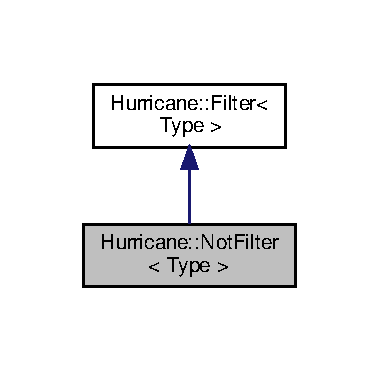
\includegraphics[width=182pt]{classHurricane_1_1NotFilter__inherit__graph}
\end{center}
\end{figure}
\doxysubsection*{Public Member Functions}
\begin{DoxyCompactItemize}
\item 
\mbox{\hyperlink{classHurricane_1_1NotFilter_a8c75f2e192929c1b559f4ca876e47126}{Not\+Filter}} (const \mbox{\hyperlink{classHurricane_1_1Filter}{Filter}}$<$ Type $>$ \&filter)
\item 
\mbox{\hyperlink{classHurricane_1_1NotFilter_a232102dc584111a704e66b2ac793af86}{Not\+Filter}} (const \mbox{\hyperlink{classHurricane_1_1NotFilter}{Not\+Filter}}$<$ Type $>$ \&not\+Filter)
\end{DoxyCompactItemize}


\doxysubsection{Detailed Description}
\subsubsection*{template$<$class Type$>$\newline
class Hurricane\+::\+Not\+Filter$<$ Type $>$}

\mbox{\hyperlink{classHurricane_1_1Filter}{Filter}} negation. 

This filter invert the matching criterion of any other filter.

\begin{DoxyRemark}{Remarks}
This is a raw \mbox{\hyperlink{classHurricane_1_1Filter}{Filter}}. 
\end{DoxyRemark}


\doxysubsection{Constructor \& Destructor Documentation}
\mbox{\Hypertarget{classHurricane_1_1NotFilter_a8c75f2e192929c1b559f4ca876e47126}\label{classHurricane_1_1NotFilter_a8c75f2e192929c1b559f4ca876e47126}} 
\index{Hurricane::NotFilter$<$ Type $>$@{Hurricane::NotFilter$<$ Type $>$}!NotFilter@{NotFilter}}
\index{NotFilter@{NotFilter}!Hurricane::NotFilter$<$ Type $>$@{Hurricane::NotFilter$<$ Type $>$}}
\doxysubsubsection{\texorpdfstring{NotFilter()}{NotFilter()}\hspace{0.1cm}{\footnotesize\ttfamily [1/2]}}
{\footnotesize\ttfamily template$<$class Type $>$ \\
\mbox{\hyperlink{classHurricane_1_1NotFilter}{Hurricane\+::\+Not\+Filter}}$<$ Type $>$\+::\mbox{\hyperlink{classHurricane_1_1NotFilter}{Not\+Filter}} (\begin{DoxyParamCaption}\item[{const \mbox{\hyperlink{classHurricane_1_1Filter}{Filter}}$<$ Type $>$ \&}]{filter }\end{DoxyParamCaption})\hspace{0.3cm}{\ttfamily [inline]}}

Constructor from a raw \mbox{\hyperlink{classHurricane_1_1Filter}{Filter}}.

\begin{DoxyRemark}{Remarks}
This constructor build a {\itshape copy} of the raw filter. So the originating filter can be safely deleted. 
\end{DoxyRemark}
\mbox{\Hypertarget{classHurricane_1_1NotFilter_a232102dc584111a704e66b2ac793af86}\label{classHurricane_1_1NotFilter_a232102dc584111a704e66b2ac793af86}} 
\index{Hurricane::NotFilter$<$ Type $>$@{Hurricane::NotFilter$<$ Type $>$}!NotFilter@{NotFilter}}
\index{NotFilter@{NotFilter}!Hurricane::NotFilter$<$ Type $>$@{Hurricane::NotFilter$<$ Type $>$}}
\doxysubsubsection{\texorpdfstring{NotFilter()}{NotFilter()}\hspace{0.1cm}{\footnotesize\ttfamily [2/2]}}
{\footnotesize\ttfamily template$<$class Type $>$ \\
\mbox{\hyperlink{classHurricane_1_1NotFilter}{Hurricane\+::\+Not\+Filter}}$<$ Type $>$\+::\mbox{\hyperlink{classHurricane_1_1NotFilter}{Not\+Filter}} (\begin{DoxyParamCaption}\item[{const \mbox{\hyperlink{classHurricane_1_1NotFilter}{Not\+Filter}}$<$ Type $>$ \&}]{filter }\end{DoxyParamCaption})\hspace{0.3cm}{\ttfamily [inline]}}

Copy constructor.

\begin{DoxyRemark}{Remarks}
This constructor build a {\itshape copy} of the raw filter. So the originating filter can be safely deleted. 
\end{DoxyRemark}


The documentation for this class was generated from the following files\+:\begin{DoxyCompactItemize}
\item 
Filter.\+h\item 
Filter.\+dox\end{DoxyCompactItemize}

\hypertarget{classHurricane_1_1Occurrence}{}\doxysection{Hurricane\+::Occurrence Class Reference}
\label{classHurricane_1_1Occurrence}\index{Hurricane::Occurrence@{Hurricane::Occurrence}}


\mbox{\hyperlink{classHurricane_1_1Occurrence}{Occurrence}} description ({\bfseries{API}})  


\doxysubsection*{Public Member Functions}
\begin{DoxyCompactItemize}
\item 
\mbox{\hyperlink{classHurricane_1_1Occurrence_aa4162a36dc984d71caf962e55b991ed0}{Occurrence}} (const \mbox{\hyperlink{classHurricane_1_1Entity}{Entity}} $\ast$entity=NULL)
\item 
\mbox{\hyperlink{classHurricane_1_1Occurrence_afedb5d75781a9a4f0a19d37f0e8c88a8}{Occurrence}} (const \mbox{\hyperlink{classHurricane_1_1Entity}{Entity}} $\ast$entity, const \mbox{\hyperlink{classHurricane_1_1Path}{Path}} \&path)
\item 
\mbox{\hyperlink{classHurricane_1_1Occurrence_affec5f25b9c2efa2bcde02e9c4833626}{Occurrence}} (const \mbox{\hyperlink{classHurricane_1_1Occurrence}{Occurrence}} \&occurrence)
\item 
\mbox{\hyperlink{classHurricane_1_1Occurrence}{Occurrence}} \& \mbox{\hyperlink{classHurricane_1_1Occurrence_a389472d0d5b121a4e091511c8003cb47}{operator=}} (const \mbox{\hyperlink{classHurricane_1_1Occurrence}{Occurrence}} \&occurrence)
\item 
bool \mbox{\hyperlink{classHurricane_1_1Occurrence_accae7f6611cb5985478d58fc793dc3e0}{operator==}} (const \mbox{\hyperlink{classHurricane_1_1Occurrence}{Occurrence}} \&occurrence) const
\item 
bool \mbox{\hyperlink{classHurricane_1_1Occurrence_a39edad19edeef964e5340381360c0add}{operator!=}} (const \mbox{\hyperlink{classHurricane_1_1Occurrence}{Occurrence}} \&occurrence) const
\item 
bool \mbox{\hyperlink{classHurricane_1_1Occurrence_a2f1668ccce22799c99eb3a02e522c204}{operator$<$}} (const \mbox{\hyperlink{classHurricane_1_1Occurrence}{Occurrence}} \&occurrence) const
\item 
\mbox{\hyperlink{classHurricane_1_1Entity}{Entity}} $\ast$ \mbox{\hyperlink{classHurricane_1_1Occurrence_ac121005d5d3bc0837f66c0de4265b0c4}{get\+Entity}} () const
\item 
\mbox{\hyperlink{classHurricane_1_1Path}{Path}} \mbox{\hyperlink{classHurricane_1_1Occurrence_adeab556806a83e8cf3ad6ecc08f3a83e}{get\+Path}} () const
\item 
\mbox{\hyperlink{classHurricane_1_1Cell}{Cell}} $\ast$ \mbox{\hyperlink{classHurricane_1_1Occurrence_affced95f35617150b5811c3784b20d93}{get\+Owner\+Cell}} () const
\item 
\mbox{\hyperlink{classHurricane_1_1Cell}{Cell}} $\ast$ \mbox{\hyperlink{classHurricane_1_1Occurrence_a5caeab69e23907909b3deb60ff26df15}{get\+Master\+Cell}} () const
\item 
\mbox{\hyperlink{classHurricane_1_1Property}{Property}} $\ast$ \mbox{\hyperlink{classHurricane_1_1Occurrence_ab2b36b219037a2310f6527a35a9a266f}{get\+Property}} (const \mbox{\hyperlink{classHurricane_1_1Name}{Name}} \&name) const
\item 
\mbox{\hyperlink{namespaceHurricane_afd7bca6dad4be54b7c03b0463e6c0004}{Properties}} \mbox{\hyperlink{classHurricane_1_1Occurrence_acbf59d6c01804e01f66d076c149abb49}{get\+Properties}} () const
\item 
\mbox{\hyperlink{classHurricane_1_1Box}{Box}} \mbox{\hyperlink{classHurricane_1_1Occurrence_a6c808dba6637c716075e0887c5f25518}{get\+Bounding\+Box}} () const
\item 
bool \mbox{\hyperlink{classHurricane_1_1Occurrence_ade38e5da7eb5d8701cd3a8f252cdf62f}{is\+Valid}} () const
\item 
bool \mbox{\hyperlink{classHurricane_1_1Occurrence_a0c1c6cfdf47f33166d108e2311d74e48}{has\+Property}} () const
\item 
void \mbox{\hyperlink{classHurricane_1_1Occurrence_aaea0bdc4f5bb4012eb52f3abe20525be}{put}} (\mbox{\hyperlink{classHurricane_1_1Property}{Property}} $\ast$property)
\item 
void \mbox{\hyperlink{classHurricane_1_1Occurrence_a774404aa5eb01371f64cf5fda3f3ffbf}{remove}} (\mbox{\hyperlink{classHurricane_1_1Property}{Property}} $\ast$property)
\item 
void \mbox{\hyperlink{classHurricane_1_1Occurrence_a8d86755bf50cbc7fd2849b039a372b0a}{remove\+Property}} (const \mbox{\hyperlink{classHurricane_1_1Name}{Name}} \&name)
\item 
void \mbox{\hyperlink{classHurricane_1_1Occurrence_ae9b269d39f3f68645d6d396d7ab5d8b7}{clear\+Properties}} ()
\end{DoxyCompactItemize}


\doxysubsection{Detailed Description}
\mbox{\hyperlink{classHurricane_1_1Occurrence}{Occurrence}} description ({\bfseries{API}}) 

\hypertarget{classHurricane_1_1Occurrence_secOccurrenceIntro}{}\doxysubsection{Introduction}\label{classHurricane_1_1Occurrence_secOccurrenceIntro}
Occurrences are objects providing the capability to designate any entity of the hierarchical assembly as if this one was virtually unfolded.

For that purpose they handle, on one side the referenced entity and on the other side the hierarchical instanciation path which refers to the cell containing this entity.

Those occurrences are handy, volatile and very light objects. Two different occurrences may designate the same entity of the virtually unfolded data structure, simplifying the creation and deletion of those objects.

Anyway it is possible to attach properties to each occurrence.

Of course, those properties are securely stored in order to access them unambiguously.

Therefore, if a property is placed on an occurrence, we have access to it from a different occurrence provided it designates the same entity of the virtually unfolded data structure.\hypertarget{classHurricane_1_1Occurrence_secOccurrenceTerminology}{}\doxysubsection{Terminology}\label{classHurricane_1_1Occurrence_secOccurrenceTerminology}
An occurrence is said invalid if it refers no entity.

When it is valid, an occurrence has \+: an {\bfseries{Owner\+Cell}} which is either the cell owning the path if this one is non void, else the cell owning the entity itself. and a {\bfseries{Master\+Cell}} which is always the cell owning the entity.\hypertarget{classHurricane_1_1Occurrence_secOccurrenceRemarks}{}\doxysubsection{Remarks}\label{classHurricane_1_1Occurrence_secOccurrenceRemarks}
All constructors, the destructor and the different operators are very efficient. 

\doxysubsection{Constructor \& Destructor Documentation}
\mbox{\Hypertarget{classHurricane_1_1Occurrence_aa4162a36dc984d71caf962e55b991ed0}\label{classHurricane_1_1Occurrence_aa4162a36dc984d71caf962e55b991ed0}} 
\index{Hurricane::Occurrence@{Hurricane::Occurrence}!Occurrence@{Occurrence}}
\index{Occurrence@{Occurrence}!Hurricane::Occurrence@{Hurricane::Occurrence}}
\doxysubsubsection{\texorpdfstring{Occurrence()}{Occurrence()}\hspace{0.1cm}{\footnotesize\ttfamily [1/3]}}
{\footnotesize\ttfamily Hurricane\+::\+Occurrence\+::\+Occurrence (\begin{DoxyParamCaption}\item[{const \mbox{\hyperlink{classHurricane_1_1Entity}{Entity}} $\ast$}]{entity = {\ttfamily NULL} }\end{DoxyParamCaption})}

Builds an occurrence refering to an entity through a void path, in some way it is equivalent to the entity itself.

\begin{DoxyRemark}{Remarks}
If the entity is null the occurrence is invalid. 
\end{DoxyRemark}
\mbox{\Hypertarget{classHurricane_1_1Occurrence_afedb5d75781a9a4f0a19d37f0e8c88a8}\label{classHurricane_1_1Occurrence_afedb5d75781a9a4f0a19d37f0e8c88a8}} 
\index{Hurricane::Occurrence@{Hurricane::Occurrence}!Occurrence@{Occurrence}}
\index{Occurrence@{Occurrence}!Hurricane::Occurrence@{Hurricane::Occurrence}}
\doxysubsubsection{\texorpdfstring{Occurrence()}{Occurrence()}\hspace{0.1cm}{\footnotesize\ttfamily [2/3]}}
{\footnotesize\ttfamily Hurricane\+::\+Occurrence\+::\+Occurrence (\begin{DoxyParamCaption}\item[{const \mbox{\hyperlink{classHurricane_1_1Entity}{Entity}} $\ast$}]{entity,  }\item[{const \mbox{\hyperlink{classHurricane_1_1Path}{Path}} \&}]{path }\end{DoxyParamCaption})}

Builds an occurrence refering to an entity through a path (possibly void).

\begin{DoxyParagraph}{Caution\+: If the entity is null or if the path is uncompatible with the }
entity, an exception is thrown.
\end{DoxyParagraph}
\begin{DoxyRemark}{Remarks}
The entity and the path are compatible if the path is void or if the master cell of the path is the cell owning the entity. 
\end{DoxyRemark}
\mbox{\Hypertarget{classHurricane_1_1Occurrence_affec5f25b9c2efa2bcde02e9c4833626}\label{classHurricane_1_1Occurrence_affec5f25b9c2efa2bcde02e9c4833626}} 
\index{Hurricane::Occurrence@{Hurricane::Occurrence}!Occurrence@{Occurrence}}
\index{Occurrence@{Occurrence}!Hurricane::Occurrence@{Hurricane::Occurrence}}
\doxysubsubsection{\texorpdfstring{Occurrence()}{Occurrence()}\hspace{0.1cm}{\footnotesize\ttfamily [3/3]}}
{\footnotesize\ttfamily Hurricane\+::\+Occurrence\+::\+Occurrence (\begin{DoxyParamCaption}\item[{const \mbox{\hyperlink{classHurricane_1_1Occurrence}{Occurrence}} \&}]{Occurrence }\end{DoxyParamCaption})}

Copy constructor. 

\doxysubsection{Member Function Documentation}
\mbox{\Hypertarget{classHurricane_1_1Occurrence_a389472d0d5b121a4e091511c8003cb47}\label{classHurricane_1_1Occurrence_a389472d0d5b121a4e091511c8003cb47}} 
\index{Hurricane::Occurrence@{Hurricane::Occurrence}!operator=@{operator=}}
\index{operator=@{operator=}!Hurricane::Occurrence@{Hurricane::Occurrence}}
\doxysubsubsection{\texorpdfstring{operator=()}{operator=()}}
{\footnotesize\ttfamily \mbox{\hyperlink{classHurricane_1_1Occurrence}{Occurrence}} \& Hurricane\+::\+Occurrence\+::operator= (\begin{DoxyParamCaption}\item[{const \mbox{\hyperlink{classHurricane_1_1Occurrence}{Occurrence}} \&}]{occurrence }\end{DoxyParamCaption})}

Assignment operator. \mbox{\Hypertarget{classHurricane_1_1Occurrence_accae7f6611cb5985478d58fc793dc3e0}\label{classHurricane_1_1Occurrence_accae7f6611cb5985478d58fc793dc3e0}} 
\index{Hurricane::Occurrence@{Hurricane::Occurrence}!operator==@{operator==}}
\index{operator==@{operator==}!Hurricane::Occurrence@{Hurricane::Occurrence}}
\doxysubsubsection{\texorpdfstring{operator==()}{operator==()}}
{\footnotesize\ttfamily bool Hurricane\+::\+Occurrence\+::operator== (\begin{DoxyParamCaption}\item[{const \mbox{\hyperlink{classHurricane_1_1Occurrence}{Occurrence}} \&}]{occurrence }\end{DoxyParamCaption}) const}

Two occurrences are equal if both are valid and refer to the same entity and have indentical instanciation pathes. \mbox{\Hypertarget{classHurricane_1_1Occurrence_a39edad19edeef964e5340381360c0add}\label{classHurricane_1_1Occurrence_a39edad19edeef964e5340381360c0add}} 
\index{Hurricane::Occurrence@{Hurricane::Occurrence}!operator"!=@{operator"!=}}
\index{operator"!=@{operator"!=}!Hurricane::Occurrence@{Hurricane::Occurrence}}
\doxysubsubsection{\texorpdfstring{operator"!=()}{operator!=()}}
{\footnotesize\ttfamily bool Hurricane\+::\+Occurrence\+::operator!= (\begin{DoxyParamCaption}\item[{const \mbox{\hyperlink{classHurricane_1_1Occurrence}{Occurrence}} \&}]{occurrence }\end{DoxyParamCaption}) const}

Two occurrences are different if a least one is either invalid or both don\textquotesingle{}t refer to the same entity or have differing instanciation pathes. \mbox{\Hypertarget{classHurricane_1_1Occurrence_a2f1668ccce22799c99eb3a02e522c204}\label{classHurricane_1_1Occurrence_a2f1668ccce22799c99eb3a02e522c204}} 
\index{Hurricane::Occurrence@{Hurricane::Occurrence}!operator$<$@{operator$<$}}
\index{operator$<$@{operator$<$}!Hurricane::Occurrence@{Hurricane::Occurrence}}
\doxysubsubsection{\texorpdfstring{operator$<$()}{operator<()}}
{\footnotesize\ttfamily bool Hurricane\+::\+Occurrence\+::operator$<$ (\begin{DoxyParamCaption}\item[{const \mbox{\hyperlink{classHurricane_1_1Occurrence}{Occurrence}} \&}]{occurrence }\end{DoxyParamCaption}) const}

This comparator has no particular signification. It is just defined to be abble to use a STL set of occurrences which need a comparator. \mbox{\Hypertarget{classHurricane_1_1Occurrence_ac121005d5d3bc0837f66c0de4265b0c4}\label{classHurricane_1_1Occurrence_ac121005d5d3bc0837f66c0de4265b0c4}} 
\index{Hurricane::Occurrence@{Hurricane::Occurrence}!getEntity@{getEntity}}
\index{getEntity@{getEntity}!Hurricane::Occurrence@{Hurricane::Occurrence}}
\doxysubsubsection{\texorpdfstring{getEntity()}{getEntity()}}
{\footnotesize\ttfamily \mbox{\hyperlink{classHurricane_1_1Entity}{Entity}} $\ast$ Hurricane\+::\+Occurrence\+::get\+Entity (\begin{DoxyParamCaption}{ }\end{DoxyParamCaption}) const\hspace{0.3cm}{\ttfamily [inline]}}

{\bfseries{Returns\+:}} the referenced entity or NULL if the occurrence is invalid. \mbox{\Hypertarget{classHurricane_1_1Occurrence_adeab556806a83e8cf3ad6ecc08f3a83e}\label{classHurricane_1_1Occurrence_adeab556806a83e8cf3ad6ecc08f3a83e}} 
\index{Hurricane::Occurrence@{Hurricane::Occurrence}!getPath@{getPath}}
\index{getPath@{getPath}!Hurricane::Occurrence@{Hurricane::Occurrence}}
\doxysubsubsection{\texorpdfstring{getPath()}{getPath()}}
{\footnotesize\ttfamily const \mbox{\hyperlink{classHurricane_1_1Path}{Path}} \& Hurricane\+::\+Occurrence\+::get\+Path (\begin{DoxyParamCaption}{ }\end{DoxyParamCaption}) const\hspace{0.3cm}{\ttfamily [inline]}}

{\bfseries{Returns\+:}} the hierarchical instanciation path of the occurrence (possibly void, but always void when the occurrence id invalid). \mbox{\Hypertarget{classHurricane_1_1Occurrence_affced95f35617150b5811c3784b20d93}\label{classHurricane_1_1Occurrence_affced95f35617150b5811c3784b20d93}} 
\index{Hurricane::Occurrence@{Hurricane::Occurrence}!getOwnerCell@{getOwnerCell}}
\index{getOwnerCell@{getOwnerCell}!Hurricane::Occurrence@{Hurricane::Occurrence}}
\doxysubsubsection{\texorpdfstring{getOwnerCell()}{getOwnerCell()}}
{\footnotesize\ttfamily \mbox{\hyperlink{classHurricane_1_1Cell}{Cell}} $\ast$ Hurricane\+::\+Occurrence\+::get\+Owner\+Cell (\begin{DoxyParamCaption}{ }\end{DoxyParamCaption}) const}

{\bfseries{Returns\+:}} the owner cell of the occurrence or NULL if the occurrence is invalid. 

Referenced by Hurricane\+::\+Hyper\+Net\+::get\+Cell().

\mbox{\Hypertarget{classHurricane_1_1Occurrence_a5caeab69e23907909b3deb60ff26df15}\label{classHurricane_1_1Occurrence_a5caeab69e23907909b3deb60ff26df15}} 
\index{Hurricane::Occurrence@{Hurricane::Occurrence}!getMasterCell@{getMasterCell}}
\index{getMasterCell@{getMasterCell}!Hurricane::Occurrence@{Hurricane::Occurrence}}
\doxysubsubsection{\texorpdfstring{getMasterCell()}{getMasterCell()}}
{\footnotesize\ttfamily \mbox{\hyperlink{classHurricane_1_1Cell}{Cell}} $\ast$ Hurricane\+::\+Occurrence\+::get\+Master\+Cell (\begin{DoxyParamCaption}{ }\end{DoxyParamCaption}) const}

{\bfseries{Returns\+:}} the cell owning the referenced entity or NULL if the occurrence is invalid. \mbox{\Hypertarget{classHurricane_1_1Occurrence_ab2b36b219037a2310f6527a35a9a266f}\label{classHurricane_1_1Occurrence_ab2b36b219037a2310f6527a35a9a266f}} 
\index{Hurricane::Occurrence@{Hurricane::Occurrence}!getProperty@{getProperty}}
\index{getProperty@{getProperty}!Hurricane::Occurrence@{Hurricane::Occurrence}}
\doxysubsubsection{\texorpdfstring{getProperty()}{getProperty()}}
{\footnotesize\ttfamily \mbox{\hyperlink{classHurricane_1_1Property}{Property}} $\ast$ Hurricane\+::\+Occurrence\+::get\+Property (\begin{DoxyParamCaption}\item[{const \mbox{\hyperlink{classHurricane_1_1Name}{Name}} \&}]{name }\end{DoxyParamCaption}) const}

{\bfseries{Returns\+:}} the property named {\ttfamily $<$name$>$} if it exists or NULL if not (or if the occurrence is invalid). \mbox{\Hypertarget{classHurricane_1_1Occurrence_acbf59d6c01804e01f66d076c149abb49}\label{classHurricane_1_1Occurrence_acbf59d6c01804e01f66d076c149abb49}} 
\index{Hurricane::Occurrence@{Hurricane::Occurrence}!getProperties@{getProperties}}
\index{getProperties@{getProperties}!Hurricane::Occurrence@{Hurricane::Occurrence}}
\doxysubsubsection{\texorpdfstring{getProperties()}{getProperties()}}
{\footnotesize\ttfamily \mbox{\hyperlink{namespaceHurricane_afd7bca6dad4be54b7c03b0463e6c0004}{Properties}} Hurricane\+::\+Occurrence\+::get\+Properties (\begin{DoxyParamCaption}{ }\end{DoxyParamCaption}) const}

{\bfseries{Returns\+:}} the collection of properties attached to the occurrence (always empty if the occurrence is invalid). \mbox{\Hypertarget{classHurricane_1_1Occurrence_a6c808dba6637c716075e0887c5f25518}\label{classHurricane_1_1Occurrence_a6c808dba6637c716075e0887c5f25518}} 
\index{Hurricane::Occurrence@{Hurricane::Occurrence}!getBoundingBox@{getBoundingBox}}
\index{getBoundingBox@{getBoundingBox}!Hurricane::Occurrence@{Hurricane::Occurrence}}
\doxysubsubsection{\texorpdfstring{getBoundingBox()}{getBoundingBox()}}
{\footnotesize\ttfamily \mbox{\hyperlink{classHurricane_1_1Box}{Box}} Hurricane\+::\+Occurrence\+::get\+Bounding\+Box (\begin{DoxyParamCaption}{ }\end{DoxyParamCaption}) const}

{\bfseries{Returns\+:}} the bounding box of the occurrence (within the coordinate sysem of the owner cell) if it is valid or else the empty box. \mbox{\Hypertarget{classHurricane_1_1Occurrence_ade38e5da7eb5d8701cd3a8f252cdf62f}\label{classHurricane_1_1Occurrence_ade38e5da7eb5d8701cd3a8f252cdf62f}} 
\index{Hurricane::Occurrence@{Hurricane::Occurrence}!isValid@{isValid}}
\index{isValid@{isValid}!Hurricane::Occurrence@{Hurricane::Occurrence}}
\doxysubsubsection{\texorpdfstring{isValid()}{isValid()}}
{\footnotesize\ttfamily bool Hurricane\+::\+Occurrence\+::is\+Valid (\begin{DoxyParamCaption}{ }\end{DoxyParamCaption}) const\hspace{0.3cm}{\ttfamily [inline]}}

{\bfseries{Returns\+:}} {\bfseries{true}} if the occurrence is valid, else {\bfseries{false}} (the occurrence refers no entity). \mbox{\Hypertarget{classHurricane_1_1Occurrence_a0c1c6cfdf47f33166d108e2311d74e48}\label{classHurricane_1_1Occurrence_a0c1c6cfdf47f33166d108e2311d74e48}} 
\index{Hurricane::Occurrence@{Hurricane::Occurrence}!hasProperty@{hasProperty}}
\index{hasProperty@{hasProperty}!Hurricane::Occurrence@{Hurricane::Occurrence}}
\doxysubsubsection{\texorpdfstring{hasProperty()}{hasProperty()}}
{\footnotesize\ttfamily bool Hurricane\+::\+Occurrence\+::has\+Property (\begin{DoxyParamCaption}{ }\end{DoxyParamCaption}) const}

{\bfseries{Returns\+:}} {\bfseries{true}} if the occurrence owns some property else {\bfseries{false}}. \mbox{\Hypertarget{classHurricane_1_1Occurrence_aaea0bdc4f5bb4012eb52f3abe20525be}\label{classHurricane_1_1Occurrence_aaea0bdc4f5bb4012eb52f3abe20525be}} 
\index{Hurricane::Occurrence@{Hurricane::Occurrence}!put@{put}}
\index{put@{put}!Hurricane::Occurrence@{Hurricane::Occurrence}}
\doxysubsubsection{\texorpdfstring{put()}{put()}}
{\footnotesize\ttfamily void Hurricane\+::\+Occurrence\+::put (\begin{DoxyParamCaption}\item[{\mbox{\hyperlink{classHurricane_1_1Property}{Property}} $\ast$}]{property }\end{DoxyParamCaption})}

Adds the property {\ttfamily $<$property$>$} to the occurrence property set. The property being named, if another property already exists in the set it will be, in a first step, detached from this set.

\begin{DoxyRemark}{Remarks}
Does nothing if the occurrence already owns this property object.
\end{DoxyRemark}
\begin{DoxyParagraph}{Caution\+: If the occurrence is invalid or the property null, an }
exception is thrown. 
\end{DoxyParagraph}
\mbox{\Hypertarget{classHurricane_1_1Occurrence_a774404aa5eb01371f64cf5fda3f3ffbf}\label{classHurricane_1_1Occurrence_a774404aa5eb01371f64cf5fda3f3ffbf}} 
\index{Hurricane::Occurrence@{Hurricane::Occurrence}!remove@{remove}}
\index{remove@{remove}!Hurricane::Occurrence@{Hurricane::Occurrence}}
\doxysubsubsection{\texorpdfstring{remove()}{remove()}}
{\footnotesize\ttfamily void Hurricane\+::\+Occurrence\+::remove (\begin{DoxyParamCaption}\item[{\mbox{\hyperlink{classHurricane_1_1Property}{Property}} $\ast$}]{property }\end{DoxyParamCaption})}

removes the property {\ttfamily $<$property$>$} from the occurrence property set.

\begin{DoxyRemark}{Remarks}
Does nothing if the occurrence doesn\textquotesingle{}t own this property object.
\end{DoxyRemark}
\begin{DoxyParagraph}{Caution\+: If the occurrence is invalid or the property null, an }
exception is thrown. 
\end{DoxyParagraph}
\mbox{\Hypertarget{classHurricane_1_1Occurrence_a8d86755bf50cbc7fd2849b039a372b0a}\label{classHurricane_1_1Occurrence_a8d86755bf50cbc7fd2849b039a372b0a}} 
\index{Hurricane::Occurrence@{Hurricane::Occurrence}!removeProperty@{removeProperty}}
\index{removeProperty@{removeProperty}!Hurricane::Occurrence@{Hurricane::Occurrence}}
\doxysubsubsection{\texorpdfstring{removeProperty()}{removeProperty()}}
{\footnotesize\ttfamily void Hurricane\+::\+Occurrence\+::remove\+Property (\begin{DoxyParamCaption}\item[{const \mbox{\hyperlink{classHurricane_1_1Name}{Name}} \&}]{name }\end{DoxyParamCaption})}

removes the property of name {\ttfamily $<$name$>$} if it exists.

\begin{DoxyParagraph}{Caution\+: If the occurrence is invalid an exception is thrown. }

\end{DoxyParagraph}
\mbox{\Hypertarget{classHurricane_1_1Occurrence_ae9b269d39f3f68645d6d396d7ab5d8b7}\label{classHurricane_1_1Occurrence_ae9b269d39f3f68645d6d396d7ab5d8b7}} 
\index{Hurricane::Occurrence@{Hurricane::Occurrence}!clearProperties@{clearProperties}}
\index{clearProperties@{clearProperties}!Hurricane::Occurrence@{Hurricane::Occurrence}}
\doxysubsubsection{\texorpdfstring{clearProperties()}{clearProperties()}}
{\footnotesize\ttfamily void Hurricane\+::\+Occurrence\+::clear\+Properties (\begin{DoxyParamCaption}{ }\end{DoxyParamCaption})}

removes all properties attached to the occurrence. As a consequence, the occurrence is deleted.

\begin{DoxyParagraph}{Caution\+: If the occurrence is invalid an exception is thrown. }

\end{DoxyParagraph}


The documentation for this class was generated from the following files\+:\begin{DoxyCompactItemize}
\item 
Occurrence.\+h\item 
Occurrence.\+dox\end{DoxyCompactItemize}

\hypertarget{classHurricane_1_1Transformation_1_1Orientation}{}\doxysection{Hurricane\+::Transformation\+::Orientation Class Reference}
\label{classHurricane_1_1Transformation_1_1Orientation}\index{Hurricane::Transformation::Orientation@{Hurricane::Transformation::Orientation}}


\doxysubsection{Detailed Description}
This enumeration defines the orientation associated to a transformation object.

\begin{center} 
\tabulinesep=1mm
\begin{longtabu}spread 0pt [c]{*{8}{|X[-1]}|}
\caption{\mbox{\hyperlink{classHurricane_1_1Transformation_1_1Orientation}{Orientation}} codes and associated transformation matrix}\label{_}\\
\hline
\cellcolor{\tableheadbgcolor}\textbf{ \begin{center}\mbox{\hyperlink{classHurricane_1_1Name}{Name}}\end{center}  }&\cellcolor{\tableheadbgcolor}\textbf{ \begin{center}Aspect\end{center}  }&\cellcolor{\tableheadbgcolor}\textbf{ \begin{center}Code\end{center}  }&\cellcolor{\tableheadbgcolor}\textbf{ \begin{center}Signification\end{center}  }&\cellcolor{\tableheadbgcolor}\textbf{ \begin{center}a\end{center}  }&\cellcolor{\tableheadbgcolor}\textbf{ \begin{center}b\end{center}  }&\cellcolor{\tableheadbgcolor}\textbf{ \begin{center}c\end{center}  }&\cellcolor{\tableheadbgcolor}\textbf{ \begin{center}d\end{center}  }\\\cline{1-8}
\endfirsthead
\hline
\endfoot
\hline
\cellcolor{\tableheadbgcolor}\textbf{ \begin{center}\mbox{\hyperlink{classHurricane_1_1Name}{Name}}\end{center}  }&\cellcolor{\tableheadbgcolor}\textbf{ \begin{center}Aspect\end{center}  }&\cellcolor{\tableheadbgcolor}\textbf{ \begin{center}Code\end{center}  }&\cellcolor{\tableheadbgcolor}\textbf{ \begin{center}Signification\end{center}  }&\cellcolor{\tableheadbgcolor}\textbf{ \begin{center}a\end{center}  }&\cellcolor{\tableheadbgcolor}\textbf{ \begin{center}b\end{center}  }&\cellcolor{\tableheadbgcolor}\textbf{ \begin{center}c\end{center}  }&\cellcolor{\tableheadbgcolor}\textbf{ \begin{center}d\end{center}  }\\\cline{1-8}
\endhead
\begin{center}{\bfseries{ID}}\end{center}  & &\begin{center}{\bfseries{0}}\end{center}  &Identity &\begin{center}1\end{center}  &\begin{center}0\end{center}  &\begin{center}0\end{center}  &\begin{center}1\end{center}  \\\cline{1-8}
\begin{center}{\bfseries{R1}}\end{center}  & &\begin{center}{\bfseries{1}}\end{center}  &Simple rotation (90�) &\begin{center}0\end{center}  &\begin{center}-\/1\end{center}  &\begin{center}1\end{center}  &\begin{center}0\end{center}  \\\cline{1-8}
\begin{center}{\bfseries{R2}}\end{center}  & &\begin{center}{\bfseries{2}}\end{center}  &Double rotation (180�) &\begin{center}-\/1\end{center}  &\begin{center}0\end{center}  &\begin{center}0\end{center}  &\begin{center}-\/1\end{center}  \\\cline{1-8}
\begin{center}{\bfseries{R3}}\end{center}  & &\begin{center}{\bfseries{3}}\end{center} &Triple rotation (270�) &\begin{center}0\end{center} &\begin{center}1\end{center} &\begin{center}-\/1\end{center} &\begin{center}0\end{center}  \\\cline{1-8}
\begin{center}{\bfseries{MX}}\end{center}  & &\begin{center}{\bfseries{4}}\end{center}  &\mbox{\hyperlink{classHurricane_1_1Horizontal}{Horizontal}} symetry (Mirror X) &\begin{center}-\/1 \end{center} &\begin{center}0 \end{center} &\begin{center}0 \end{center} &\begin{center}1\end{center}  \\\cline{1-8}
\begin{center}{\bfseries{XR}}\end{center}  & &\begin{center}{\bfseries{5}}\end{center} &\mbox{\hyperlink{classHurricane_1_1Horizontal}{Horizontal}} symetry followed by a 90� rotation &\begin{center}0\end{center}  &\begin{center}-\/1\end{center}  &\begin{center}-\/1\end{center}  &\begin{center}0\end{center}  \\\cline{1-8}
\begin{center}{\bfseries{MY}}\end{center} & &\begin{center}{\bfseries{6}}\end{center} &\mbox{\hyperlink{classHurricane_1_1Vertical}{Vertical}} symetry (Mirror Y) &\begin{center}1\end{center}  &\begin{center}0\end{center}  &\begin{center}0\end{center}  &\begin{center}-\/1\end{center}  \\\cline{1-8}
\begin{center}{\bfseries{YR}}\end{center}  & &\begin{center}{\bfseries{7}}\end{center} &\mbox{\hyperlink{classHurricane_1_1Vertical}{Vertical}} symetry followed by a 90� rotation &\begin{center}0\end{center}  &\begin{center}1\end{center}  &\begin{center}1\end{center}  &\begin{center}0\end{center}  \\\cline{1-8}
\end{longtabu}
\end{center} 

The transformation formula is given by\+: \[ \Large \left \{ \begin{array}{r c l l l l l} x\textnormal{\textquotesingle} & = & (a \times x) & + & (b \times y) & + & tx \\ y\textnormal{\textquotesingle} & = & (c \times x) & + & (d \times y) & + & ty \end{array} \right . \] where x and y are the coordinates of any point, x\textquotesingle{} and y\textquotesingle{} the coordinates of the transformed point, tx and ty the horizontal and vertical components of the translation and where a, b, c and d are the coefficients of the matrix associated to the orientation. 

The documentation for this class was generated from the following file\+:\begin{DoxyCompactItemize}
\item 
Transformation.\+h\end{DoxyCompactItemize}

\hypertarget{classHurricane_1_1Pad}{}\doxysection{Hurricane\+::Pad Class Reference}
\label{classHurricane_1_1Pad}\index{Hurricane::Pad@{Hurricane::Pad}}


\mbox{\hyperlink{classHurricane_1_1Pad}{Pad}} description ({\bfseries{API}})  




Inheritance diagram for Hurricane\+::Pad\+:\nopagebreak
\begin{figure}[H]
\begin{center}
\leavevmode
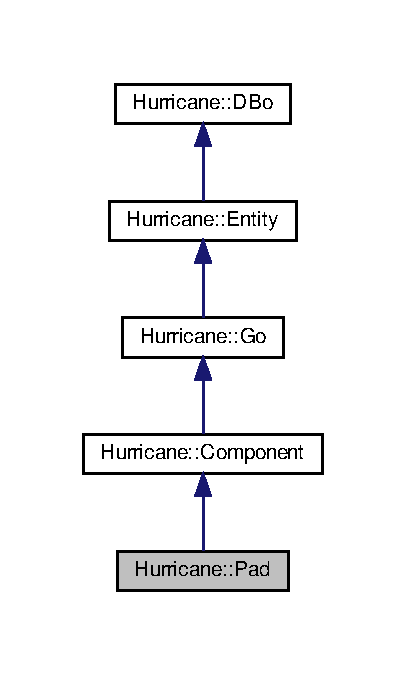
\includegraphics[width=195pt]{classHurricane_1_1Pad__inherit__graph}
\end{center}
\end{figure}
\doxysubsection*{Public Types}
\begin{DoxyCompactItemize}
\item 
typedef \mbox{\hyperlink{classHurricane_1_1Component}{Component}} \mbox{\hyperlink{classHurricane_1_1Pad_aa44130a291ce3cb878d749fbf3e5437e}{Inherit}}
\end{DoxyCompactItemize}
\doxysubsection*{Static Public Member Functions}
\begin{DoxyCompactItemize}
\item 
static \mbox{\hyperlink{classHurricane_1_1Pad}{Pad}} $\ast$ \mbox{\hyperlink{classHurricane_1_1Pad_a0fdf586f9f815d375f54b40bfa027b24}{create}} (\mbox{\hyperlink{classHurricane_1_1Net}{Net}} $\ast$net, const \mbox{\hyperlink{classHurricane_1_1Layer}{Layer}} $\ast$layer, const \mbox{\hyperlink{classHurricane_1_1Box}{Box}} \&bounding\+Box)
\end{DoxyCompactItemize}
\doxysubsection*{Additional Inherited Members}


\doxysubsection{Detailed Description}
\mbox{\hyperlink{classHurricane_1_1Pad}{Pad}} description ({\bfseries{API}}) 

\hypertarget{classHurricane_1_1Pad_secPadIntro}{}\doxysubsection{Introduction}\label{classHurricane_1_1Pad_secPadIntro}
A pad is an object representing a layout rectangle. 

\doxysubsection{Member Typedef Documentation}
\mbox{\Hypertarget{classHurricane_1_1Pad_aa44130a291ce3cb878d749fbf3e5437e}\label{classHurricane_1_1Pad_aa44130a291ce3cb878d749fbf3e5437e}} 
\index{Hurricane::Pad@{Hurricane::Pad}!Inherit@{Inherit}}
\index{Inherit@{Inherit}!Hurricane::Pad@{Hurricane::Pad}}
\doxysubsubsection{\texorpdfstring{Inherit}{Inherit}}
{\footnotesize\ttfamily \mbox{\hyperlink{classHurricane_1_1Pad_aa44130a291ce3cb878d749fbf3e5437e}{Hurricane\+::\+Pad\+::\+Inherit}}}

Useful for calling upon methods of the base class without knowing it. 

\doxysubsection{Member Function Documentation}
\mbox{\Hypertarget{classHurricane_1_1Pad_a0fdf586f9f815d375f54b40bfa027b24}\label{classHurricane_1_1Pad_a0fdf586f9f815d375f54b40bfa027b24}} 
\index{Hurricane::Pad@{Hurricane::Pad}!create@{create}}
\index{create@{create}!Hurricane::Pad@{Hurricane::Pad}}
\doxysubsubsection{\texorpdfstring{create()}{create()}}
{\footnotesize\ttfamily \mbox{\hyperlink{classHurricane_1_1Pad}{Pad}} $\ast$ Hurricane\+::\+Pad\+::create (\begin{DoxyParamCaption}\item[{\mbox{\hyperlink{classHurricane_1_1Net}{Net}} $\ast$}]{net,  }\item[{const \mbox{\hyperlink{classHurricane_1_1Layer}{Layer}} $\ast$}]{layer,  }\item[{const \mbox{\hyperlink{classHurricane_1_1Box}{Box}} \&}]{bounding\+Box }\end{DoxyParamCaption})\hspace{0.3cm}{\ttfamily [static]}}

No description. 

The documentation for this class was generated from the following files\+:\begin{DoxyCompactItemize}
\item 
Pad.\+h\item 
Pad.\+dox\end{DoxyCompactItemize}

\hypertarget{classHurricane_1_1Path}{}\doxysection{Hurricane\+::Path Class Reference}
\label{classHurricane_1_1Path}\index{Hurricane::Path@{Hurricane::Path}}


\mbox{\hyperlink{classHurricane_1_1Path}{Path}} description ({\bfseries{API}})  


\doxysubsection*{Public Member Functions}
\begin{DoxyCompactItemize}
\item 
\mbox{\hyperlink{classHurricane_1_1Path_ad3fe735dcb2ce630f89b98c039663c23}{Path}} (Shared\+Path $\ast$shared\+Path=NULL)
\item 
\mbox{\hyperlink{classHurricane_1_1Path_aa1a70f922b9b6a78fd3ac9b7bd94d158}{Path}} (\mbox{\hyperlink{classHurricane_1_1Instance}{Instance}} $\ast$instance)
\item 
\mbox{\hyperlink{classHurricane_1_1Path_a3197a114ed98117dde0f41d999917775}{Path}} (\mbox{\hyperlink{classHurricane_1_1Instance}{Instance}} $\ast$head\+Instance, const \mbox{\hyperlink{classHurricane_1_1Path}{Path}} \&tail\+Path)
\item 
\mbox{\hyperlink{classHurricane_1_1Path_add5812ab3bb9a4cf6dbe49d1e4e932cb}{Path}} (const \mbox{\hyperlink{classHurricane_1_1Path}{Path}} \&head\+Path, \mbox{\hyperlink{classHurricane_1_1Instance}{Instance}} $\ast$tail\+Instance)
\item 
\mbox{\hyperlink{classHurricane_1_1Path_a6e3d331f5c5a0dcb91d10516a4beb6bc}{Path}} (\mbox{\hyperlink{classHurricane_1_1Cell}{Cell}} $\ast$cell, const string \&path\+Name)
\item 
\mbox{\hyperlink{classHurricane_1_1Path_a8db875f788013ec5ad8ed517cf1e1715}{Path}} (const \mbox{\hyperlink{classHurricane_1_1Path}{Path}} \&path)
\item 
\mbox{\hyperlink{classHurricane_1_1Path_a6226639f50213598ffad86031afe69ff}{$\sim$\+Path}} ()
\item 
\mbox{\hyperlink{classHurricane_1_1Path}{Path}} \& \mbox{\hyperlink{classHurricane_1_1Path_a1355dd2d191d492a1b5e5180324a9f8f}{operator=}} (const \mbox{\hyperlink{classHurricane_1_1Path}{Path}} \&path)
\item 
bool \mbox{\hyperlink{classHurricane_1_1Path_a16a5b6529dd4424c55518ac9f687862f}{operator==}} (const \mbox{\hyperlink{classHurricane_1_1Path}{Path}} \&path) const
\item 
bool \mbox{\hyperlink{classHurricane_1_1Path_a182e82a2bc3f41262e1e76fcdc5a0c1e}{operator!=}} (const \mbox{\hyperlink{classHurricane_1_1Path}{Path}} \&path) const
\item 
bool \mbox{\hyperlink{classHurricane_1_1Path_a5bf33d2d9e3e7d46db770e26c09be90b}{operator$<$}} (const \mbox{\hyperlink{classHurricane_1_1Path}{Path}} \&path) const
\item 
\mbox{\hyperlink{classHurricane_1_1Instance}{Instance}} $\ast$ \mbox{\hyperlink{classHurricane_1_1Path_afddde635f302cee0a215ca364e9689b5}{get\+Head\+Instance}} () const
\item 
\mbox{\hyperlink{classHurricane_1_1Path}{Path}} \mbox{\hyperlink{classHurricane_1_1Path_af0b27566643cc252d9a0feb1709d3180}{get\+Tail\+Path}} () const
\item 
\mbox{\hyperlink{classHurricane_1_1Path}{Path}} \mbox{\hyperlink{classHurricane_1_1Path_ae89034b297b27545cf3865e0cfa31f3d}{get\+Head\+Path}} () const
\item 
\mbox{\hyperlink{classHurricane_1_1Instance}{Instance}} $\ast$ \mbox{\hyperlink{classHurricane_1_1Path_a1f9350514c4751b54b2f01082a93e3bf}{get\+Tail\+Instance}} () const
\item 
string \mbox{\hyperlink{classHurricane_1_1Path_a97ff25c53f4e7bdacb7cb8a58adf6499}{get\+Name}} () const
\item 
\mbox{\hyperlink{classHurricane_1_1Cell}{Cell}} $\ast$ \mbox{\hyperlink{classHurricane_1_1Path_a0954eb842af9d863ea701aa0b681412e}{get\+Owner\+Cell}} () const
\item 
\mbox{\hyperlink{classHurricane_1_1Cell}{Cell}} $\ast$ \mbox{\hyperlink{classHurricane_1_1Path_a3f4a865f570375ec5b6e5cb487369696}{get\+Master\+Cell}} () const
\item 
\mbox{\hyperlink{namespaceHurricane_ac9436b03a2926f34ad6863deae2baadc}{Instances}} \mbox{\hyperlink{classHurricane_1_1Path_af820422a686ab35d611a6c1969e37e90}{get\+Instances}} () const
\item 
\mbox{\hyperlink{classHurricane_1_1Transformation}{Transformation}} \mbox{\hyperlink{classHurricane_1_1Path_af48dc47810f65e7aba6ee8f24ed8a09e}{get\+Transformation}} (const \mbox{\hyperlink{classHurricane_1_1Transformation}{Transformation}} \&transformation=\mbox{\hyperlink{classHurricane_1_1Transformation}{Transformation}}()) const
\item 
bool \mbox{\hyperlink{classHurricane_1_1Path_aeddd764b4b10c72630ee81119614935a}{is\+Empty}} () const
\end{DoxyCompactItemize}
\doxysubsection*{Static Public Member Functions}
\begin{DoxyCompactItemize}
\item 
static char \mbox{\hyperlink{classHurricane_1_1Path_ac63015239df43b8c44a6d74a262eb3a2}{get\+Name\+Separator}} ()
\item 
static void \mbox{\hyperlink{classHurricane_1_1Path_a505231a4bf7e8041c7a01e482505cd7a}{set\+Name\+Separator}} (char name\+Separator)
\end{DoxyCompactItemize}


\doxysubsection{Detailed Description}
\mbox{\hyperlink{classHurricane_1_1Path}{Path}} description ({\bfseries{API}}) 

\hypertarget{classHurricane_1_1Path_secPathIntro}{}\doxysubsection{Introduction}\label{classHurricane_1_1Path_secPathIntro}
Pathes are objects representing an ordered sequence of instances through the hierarchy.

They are represented by a head instance which defines the path start and tail path which defines the remaining path with respect to the cell model referenced by the head instance.

terminology A non void path begins by an instance \+: this instance pertains to the top caller cell, named Owner\+Cell. On the other hand the path ends by an instance (which may be the same) \+: this instance refers to its model which will be named the Master\+Cell.\hypertarget{classHurricane_1_1Path_secPathRemarks}{}\doxysubsection{Remarks}\label{classHurricane_1_1Path_secPathRemarks}
The different constructors (appart the one which analyses the names of the path) as welle as the destructor and the different operators are very efficient because the tail pathes being shared, only pointer assignments and pointer comparisons are realized. 

\doxysubsection{Constructor \& Destructor Documentation}
\mbox{\Hypertarget{classHurricane_1_1Path_ad3fe735dcb2ce630f89b98c039663c23}\label{classHurricane_1_1Path_ad3fe735dcb2ce630f89b98c039663c23}} 
\index{Hurricane::Path@{Hurricane::Path}!Path@{Path}}
\index{Path@{Path}!Hurricane::Path@{Hurricane::Path}}
\doxysubsubsection{\texorpdfstring{Path()}{Path()}\hspace{0.1cm}{\footnotesize\ttfamily [1/6]}}
{\footnotesize\ttfamily Hurricane\+::\+Path\+::\+Path (\begin{DoxyParamCaption}\item[{Shared\+Path $\ast$}]{shared\+Path = {\ttfamily NULL} }\end{DoxyParamCaption})}

Default constructor \+: the path is then void.

\begin{DoxyRemark}{Remarks}
This path has no instance and will be the tail terminal path of any other path. 
\end{DoxyRemark}
\mbox{\Hypertarget{classHurricane_1_1Path_aa1a70f922b9b6a78fd3ac9b7bd94d158}\label{classHurricane_1_1Path_aa1a70f922b9b6a78fd3ac9b7bd94d158}} 
\index{Hurricane::Path@{Hurricane::Path}!Path@{Path}}
\index{Path@{Path}!Hurricane::Path@{Hurricane::Path}}
\doxysubsubsection{\texorpdfstring{Path()}{Path()}\hspace{0.1cm}{\footnotesize\ttfamily [2/6]}}
{\footnotesize\ttfamily Hurricane\+::\+Path\+::\+Path (\begin{DoxyParamCaption}\item[{\mbox{\hyperlink{classHurricane_1_1Instance}{Instance}} $\ast$}]{instance }\end{DoxyParamCaption})}

Builds the path made up of this unique instance.

\begin{DoxyParagraph}{Caution\+: If the instance is null an exception is thrown. }

\end{DoxyParagraph}
\mbox{\Hypertarget{classHurricane_1_1Path_a3197a114ed98117dde0f41d999917775}\label{classHurricane_1_1Path_a3197a114ed98117dde0f41d999917775}} 
\index{Hurricane::Path@{Hurricane::Path}!Path@{Path}}
\index{Path@{Path}!Hurricane::Path@{Hurricane::Path}}
\doxysubsubsection{\texorpdfstring{Path()}{Path()}\hspace{0.1cm}{\footnotesize\ttfamily [3/6]}}
{\footnotesize\ttfamily Hurricane\+::\+Path\+::\+Path (\begin{DoxyParamCaption}\item[{\mbox{\hyperlink{classHurricane_1_1Instance}{Instance}} $\ast$}]{head\+Instance,  }\item[{const \mbox{\hyperlink{classHurricane_1_1Path}{Path}} \&}]{tail\+Path }\end{DoxyParamCaption})}

Builds the path with head instance {\ttfamily $<$head\+Instance$>$} and tail path {\ttfamily $<$tail\+Path$>$}.

\begin{DoxyParagraph}{Caution\+: If the instance is null, or if the tail path is not }
compatible with this head instance, an exception is thrown.
\end{DoxyParagraph}
\begin{DoxyRemark}{Remarks}
The head instance and the tail path are compatible if the tail path is void or if the owner cell of the tail path is the model cell referenced by the head instance. 
\end{DoxyRemark}
\mbox{\Hypertarget{classHurricane_1_1Path_add5812ab3bb9a4cf6dbe49d1e4e932cb}\label{classHurricane_1_1Path_add5812ab3bb9a4cf6dbe49d1e4e932cb}} 
\index{Hurricane::Path@{Hurricane::Path}!Path@{Path}}
\index{Path@{Path}!Hurricane::Path@{Hurricane::Path}}
\doxysubsubsection{\texorpdfstring{Path()}{Path()}\hspace{0.1cm}{\footnotesize\ttfamily [4/6]}}
{\footnotesize\ttfamily Hurricane\+::\+Path\+::\+Path (\begin{DoxyParamCaption}\item[{const \mbox{\hyperlink{classHurricane_1_1Path}{Path}} \&}]{head\+Path,  }\item[{\mbox{\hyperlink{classHurricane_1_1Instance}{Instance}} $\ast$}]{tail\+Instance }\end{DoxyParamCaption})}

Builds the path with head path {\ttfamily $<$head\+Path$>$} and tail instance {\ttfamily $<$tail\+Instance$>$}.

\begin{DoxyParagraph}{Caution\+: If the tail instance is null, or if the head path is not }
compatible with this tail instance, an exception is thrown.
\end{DoxyParagraph}
\begin{DoxyRemark}{Remarks}
The tail instance and the head path are compatible if the owner cell of the tail instance is the master cell of the head path (which is recall it, the model cell referenced by the last instance of the head path) or if the head path is empty (then compatible with any non null instance). 
\end{DoxyRemark}
\mbox{\Hypertarget{classHurricane_1_1Path_a6e3d331f5c5a0dcb91d10516a4beb6bc}\label{classHurricane_1_1Path_a6e3d331f5c5a0dcb91d10516a4beb6bc}} 
\index{Hurricane::Path@{Hurricane::Path}!Path@{Path}}
\index{Path@{Path}!Hurricane::Path@{Hurricane::Path}}
\doxysubsubsection{\texorpdfstring{Path()}{Path()}\hspace{0.1cm}{\footnotesize\ttfamily [5/6]}}
{\footnotesize\ttfamily Hurricane\+::\+Path\+::\+Path (\begin{DoxyParamCaption}\item[{\mbox{\hyperlink{classHurricane_1_1Cell}{Cell}} $\ast$}]{cell,  }\item[{const string \&}]{path\+Name }\end{DoxyParamCaption})}

Builds the path representing the logic sequence of instance names described as a character string. Each instance name is separated from the preceeding one by a special delimiter (which can be defined with the function {\bfseries{set\+Path\+Name\+Separator}} to be defined later). The cell given in argument defines where sarts the search (at each new instance identified, we go to its model cell to pursue the search within the {\ttfamily $<$path\+Name$>$}).

\begin{DoxyParagraph}{Caution\+: If the cell is null or if the name doesn\textquotesingle{}t correspond to an }
existing hierarchical instanciation path an exception is thrown. 
\end{DoxyParagraph}
\mbox{\Hypertarget{classHurricane_1_1Path_a8db875f788013ec5ad8ed517cf1e1715}\label{classHurricane_1_1Path_a8db875f788013ec5ad8ed517cf1e1715}} 
\index{Hurricane::Path@{Hurricane::Path}!Path@{Path}}
\index{Path@{Path}!Hurricane::Path@{Hurricane::Path}}
\doxysubsubsection{\texorpdfstring{Path()}{Path()}\hspace{0.1cm}{\footnotesize\ttfamily [6/6]}}
{\footnotesize\ttfamily Hurricane\+::\+Path\+::\+Path (\begin{DoxyParamCaption}\item[{const \mbox{\hyperlink{classHurricane_1_1Path}{Path}} \&}]{path }\end{DoxyParamCaption})}

Copy constructor. \mbox{\Hypertarget{classHurricane_1_1Path_a6226639f50213598ffad86031afe69ff}\label{classHurricane_1_1Path_a6226639f50213598ffad86031afe69ff}} 
\index{Hurricane::Path@{Hurricane::Path}!````~Path@{$\sim$Path}}
\index{````~Path@{$\sim$Path}!Hurricane::Path@{Hurricane::Path}}
\doxysubsubsection{\texorpdfstring{$\sim$Path()}{~Path()}}
{\footnotesize\ttfamily Hurricane\+::\+Path\+::$\sim$\+Path (\begin{DoxyParamCaption}{ }\end{DoxyParamCaption})}

No description. 

\doxysubsection{Member Function Documentation}
\mbox{\Hypertarget{classHurricane_1_1Path_a1355dd2d191d492a1b5e5180324a9f8f}\label{classHurricane_1_1Path_a1355dd2d191d492a1b5e5180324a9f8f}} 
\index{Hurricane::Path@{Hurricane::Path}!operator=@{operator=}}
\index{operator=@{operator=}!Hurricane::Path@{Hurricane::Path}}
\doxysubsubsection{\texorpdfstring{operator=()}{operator=()}}
{\footnotesize\ttfamily \mbox{\hyperlink{classHurricane_1_1Path}{Path}} \& Hurricane\+::\+Path\+::operator= (\begin{DoxyParamCaption}\item[{const \mbox{\hyperlink{classHurricane_1_1Path}{Path}} \&}]{path }\end{DoxyParamCaption})}

Assignment operator. \mbox{\Hypertarget{classHurricane_1_1Path_a16a5b6529dd4424c55518ac9f687862f}\label{classHurricane_1_1Path_a16a5b6529dd4424c55518ac9f687862f}} 
\index{Hurricane::Path@{Hurricane::Path}!operator==@{operator==}}
\index{operator==@{operator==}!Hurricane::Path@{Hurricane::Path}}
\doxysubsubsection{\texorpdfstring{operator==()}{operator==()}}
{\footnotesize\ttfamily bool Hurricane\+::\+Path\+::operator== (\begin{DoxyParamCaption}\item[{const \mbox{\hyperlink{classHurricane_1_1Path}{Path}} \&}]{path }\end{DoxyParamCaption}) const}

Two pathes are equal if they have the same head instance and if their tail pathes are equal. \mbox{\Hypertarget{classHurricane_1_1Path_a182e82a2bc3f41262e1e76fcdc5a0c1e}\label{classHurricane_1_1Path_a182e82a2bc3f41262e1e76fcdc5a0c1e}} 
\index{Hurricane::Path@{Hurricane::Path}!operator"!=@{operator"!=}}
\index{operator"!=@{operator"!=}!Hurricane::Path@{Hurricane::Path}}
\doxysubsubsection{\texorpdfstring{operator"!=()}{operator!=()}}
{\footnotesize\ttfamily bool Hurricane\+::\+Path\+::operator!= (\begin{DoxyParamCaption}\item[{const \mbox{\hyperlink{classHurricane_1_1Path}{Path}} \&}]{path }\end{DoxyParamCaption}) const}

Two pathes are differents either if they have different head instance or if the tail pathes differ. \mbox{\Hypertarget{classHurricane_1_1Path_a5bf33d2d9e3e7d46db770e26c09be90b}\label{classHurricane_1_1Path_a5bf33d2d9e3e7d46db770e26c09be90b}} 
\index{Hurricane::Path@{Hurricane::Path}!operator$<$@{operator$<$}}
\index{operator$<$@{operator$<$}!Hurricane::Path@{Hurricane::Path}}
\doxysubsubsection{\texorpdfstring{operator$<$()}{operator<()}}
{\footnotesize\ttfamily bool Hurricane\+::\+Path\+::operator$<$ (\begin{DoxyParamCaption}\item[{const \mbox{\hyperlink{classHurricane_1_1Path}{Path}} \&}]{path }\end{DoxyParamCaption}) const}

This comparator has no particular signification. It is just defined to be abble to use a STL set of pathes which need a comparator. \mbox{\Hypertarget{classHurricane_1_1Path_ac63015239df43b8c44a6d74a262eb3a2}\label{classHurricane_1_1Path_ac63015239df43b8c44a6d74a262eb3a2}} 
\index{Hurricane::Path@{Hurricane::Path}!getNameSeparator@{getNameSeparator}}
\index{getNameSeparator@{getNameSeparator}!Hurricane::Path@{Hurricane::Path}}
\doxysubsubsection{\texorpdfstring{getNameSeparator()}{getNameSeparator()}}
{\footnotesize\ttfamily char Hurricane\+::\+Path\+::get\+Name\+Separator (\begin{DoxyParamCaption}{ }\end{DoxyParamCaption})\hspace{0.3cm}{\ttfamily [static]}}

{\bfseries{Returns\+:}} the special character used as a separator between the instance names of a path. By default it is the \textquotesingle{}.\textquotesingle{} (point). \mbox{\Hypertarget{classHurricane_1_1Path_afddde635f302cee0a215ca364e9689b5}\label{classHurricane_1_1Path_afddde635f302cee0a215ca364e9689b5}} 
\index{Hurricane::Path@{Hurricane::Path}!getHeadInstance@{getHeadInstance}}
\index{getHeadInstance@{getHeadInstance}!Hurricane::Path@{Hurricane::Path}}
\doxysubsubsection{\texorpdfstring{getHeadInstance()}{getHeadInstance()}}
{\footnotesize\ttfamily \mbox{\hyperlink{classHurricane_1_1Instance}{Instance}} $\ast$ Hurricane\+::\+Path\+::get\+Head\+Instance (\begin{DoxyParamCaption}{ }\end{DoxyParamCaption}) const}

{\bfseries{Returns\+:}} the head instance or NULL if the path is void. \mbox{\Hypertarget{classHurricane_1_1Path_af0b27566643cc252d9a0feb1709d3180}\label{classHurricane_1_1Path_af0b27566643cc252d9a0feb1709d3180}} 
\index{Hurricane::Path@{Hurricane::Path}!getTailPath@{getTailPath}}
\index{getTailPath@{getTailPath}!Hurricane::Path@{Hurricane::Path}}
\doxysubsubsection{\texorpdfstring{getTailPath()}{getTailPath()}}
{\footnotesize\ttfamily \mbox{\hyperlink{classHurricane_1_1Path}{Path}} Hurricane\+::\+Path\+::get\+Tail\+Path (\begin{DoxyParamCaption}{ }\end{DoxyParamCaption}) const}

{\bfseries{Returns\+:}} the tail path or a void path if the path has 1 or 0 hierarchical depth. \mbox{\Hypertarget{classHurricane_1_1Path_ae89034b297b27545cf3865e0cfa31f3d}\label{classHurricane_1_1Path_ae89034b297b27545cf3865e0cfa31f3d}} 
\index{Hurricane::Path@{Hurricane::Path}!getHeadPath@{getHeadPath}}
\index{getHeadPath@{getHeadPath}!Hurricane::Path@{Hurricane::Path}}
\doxysubsubsection{\texorpdfstring{getHeadPath()}{getHeadPath()}}
{\footnotesize\ttfamily \mbox{\hyperlink{classHurricane_1_1Path}{Path}} Hurricane\+::\+Path\+::get\+Head\+Path (\begin{DoxyParamCaption}{ }\end{DoxyParamCaption}) const}

{\bfseries{Returns\+:}} the head path or a void path if the path has 1 or 0 hierarchical depth. \mbox{\Hypertarget{classHurricane_1_1Path_a1f9350514c4751b54b2f01082a93e3bf}\label{classHurricane_1_1Path_a1f9350514c4751b54b2f01082a93e3bf}} 
\index{Hurricane::Path@{Hurricane::Path}!getTailInstance@{getTailInstance}}
\index{getTailInstance@{getTailInstance}!Hurricane::Path@{Hurricane::Path}}
\doxysubsubsection{\texorpdfstring{getTailInstance()}{getTailInstance()}}
{\footnotesize\ttfamily \mbox{\hyperlink{classHurricane_1_1Instance}{Instance}} $\ast$ Hurricane\+::\+Path\+::get\+Tail\+Instance (\begin{DoxyParamCaption}{ }\end{DoxyParamCaption}) const}

{\bfseries{Returns\+:}} the tail instance or NULL if the path is void. \mbox{\Hypertarget{classHurricane_1_1Path_a97ff25c53f4e7bdacb7cb8a58adf6499}\label{classHurricane_1_1Path_a97ff25c53f4e7bdacb7cb8a58adf6499}} 
\index{Hurricane::Path@{Hurricane::Path}!getName@{getName}}
\index{getName@{getName}!Hurricane::Path@{Hurricane::Path}}
\doxysubsubsection{\texorpdfstring{getName()}{getName()}}
{\footnotesize\ttfamily string Hurricane\+::\+Path\+::get\+Name (\begin{DoxyParamCaption}{ }\end{DoxyParamCaption}) const}

{\bfseries{Returns\+:}} a string defined by the concatenation of instance names separated by a special character (which can be set up by the function {\bfseries{set\+Path\+Name\+Separator}}).

{\bfseries{Returns\+:}} the string {\bfseries{\char`\"{}\char`\"{}}} when the path is void. \mbox{\Hypertarget{classHurricane_1_1Path_a0954eb842af9d863ea701aa0b681412e}\label{classHurricane_1_1Path_a0954eb842af9d863ea701aa0b681412e}} 
\index{Hurricane::Path@{Hurricane::Path}!getOwnerCell@{getOwnerCell}}
\index{getOwnerCell@{getOwnerCell}!Hurricane::Path@{Hurricane::Path}}
\doxysubsubsection{\texorpdfstring{getOwnerCell()}{getOwnerCell()}}
{\footnotesize\ttfamily \mbox{\hyperlink{classHurricane_1_1Cell}{Cell}} $\ast$ Hurricane\+::\+Path\+::get\+Owner\+Cell (\begin{DoxyParamCaption}{ }\end{DoxyParamCaption}) const}

Retruns the cell owning the head instance or NULL if the path is void. \mbox{\Hypertarget{classHurricane_1_1Path_a3f4a865f570375ec5b6e5cb487369696}\label{classHurricane_1_1Path_a3f4a865f570375ec5b6e5cb487369696}} 
\index{Hurricane::Path@{Hurricane::Path}!getMasterCell@{getMasterCell}}
\index{getMasterCell@{getMasterCell}!Hurricane::Path@{Hurricane::Path}}
\doxysubsubsection{\texorpdfstring{getMasterCell()}{getMasterCell()}}
{\footnotesize\ttfamily \mbox{\hyperlink{classHurricane_1_1Cell}{Cell}} $\ast$ Hurricane\+::\+Path\+::get\+Master\+Cell (\begin{DoxyParamCaption}{ }\end{DoxyParamCaption}) const}

{\bfseries{Returns\+:}} the master cell referenced by the last instance of the path or NULL if the path is void. \mbox{\Hypertarget{classHurricane_1_1Path_af820422a686ab35d611a6c1969e37e90}\label{classHurricane_1_1Path_af820422a686ab35d611a6c1969e37e90}} 
\index{Hurricane::Path@{Hurricane::Path}!getInstances@{getInstances}}
\index{getInstances@{getInstances}!Hurricane::Path@{Hurricane::Path}}
\doxysubsubsection{\texorpdfstring{getInstances()}{getInstances()}}
{\footnotesize\ttfamily \mbox{\hyperlink{namespaceHurricane_ac9436b03a2926f34ad6863deae2baadc}{Instances}} Hurricane\+::\+Path\+::get\+Instances (\begin{DoxyParamCaption}{ }\end{DoxyParamCaption}) const}

{\bfseries{Returns\+:}} the collection of instances defining the path. \mbox{\Hypertarget{classHurricane_1_1Path_af48dc47810f65e7aba6ee8f24ed8a09e}\label{classHurricane_1_1Path_af48dc47810f65e7aba6ee8f24ed8a09e}} 
\index{Hurricane::Path@{Hurricane::Path}!getTransformation@{getTransformation}}
\index{getTransformation@{getTransformation}!Hurricane::Path@{Hurricane::Path}}
\doxysubsubsection{\texorpdfstring{getTransformation()}{getTransformation()}}
{\footnotesize\ttfamily \mbox{\hyperlink{classHurricane_1_1Transformation}{Transformation}} Hurricane\+::\+Path\+::get\+Transformation (\begin{DoxyParamCaption}\item[{const \mbox{\hyperlink{classHurricane_1_1Transformation}{Transformation}} \&}]{transformation = {\ttfamily \mbox{\hyperlink{classHurricane_1_1Transformation}{Transformation}}()} }\end{DoxyParamCaption}) const}

{\bfseries{Returns\+:}} the transform resulting of the composition of all transforms associated with the different instances of the path, applied to the given {\ttfamily $<$transformation$>$}. \mbox{\Hypertarget{classHurricane_1_1Path_aeddd764b4b10c72630ee81119614935a}\label{classHurricane_1_1Path_aeddd764b4b10c72630ee81119614935a}} 
\index{Hurricane::Path@{Hurricane::Path}!isEmpty@{isEmpty}}
\index{isEmpty@{isEmpty}!Hurricane::Path@{Hurricane::Path}}
\doxysubsubsection{\texorpdfstring{isEmpty()}{isEmpty()}}
{\footnotesize\ttfamily bool Hurricane\+::\+Path\+::is\+Empty (\begin{DoxyParamCaption}{ }\end{DoxyParamCaption}) const}

{\bfseries{Returns\+:}} {\bfseries{true}} if the path is void and else {\bfseries{false}}. \mbox{\Hypertarget{classHurricane_1_1Path_a505231a4bf7e8041c7a01e482505cd7a}\label{classHurricane_1_1Path_a505231a4bf7e8041c7a01e482505cd7a}} 
\index{Hurricane::Path@{Hurricane::Path}!setNameSeparator@{setNameSeparator}}
\index{setNameSeparator@{setNameSeparator}!Hurricane::Path@{Hurricane::Path}}
\doxysubsubsection{\texorpdfstring{setNameSeparator()}{setNameSeparator()}}
{\footnotesize\ttfamily void Hurricane\+::\+Path\+::set\+Name\+Separator (\begin{DoxyParamCaption}\item[{char}]{separator }\end{DoxyParamCaption})\hspace{0.3cm}{\ttfamily [static]}}

This function sets the special character used as a separator between the instance names of a path (choose it carrefully, it must not appear in any instance name). 

The documentation for this class was generated from the following files\+:\begin{DoxyCompactItemize}
\item 
Path.\+h\item 
Path.\+dox\end{DoxyCompactItemize}

\hypertarget{classHurricane_1_1PhysicalRule}{}\doxysection{Hurricane\+::Physical\+Rule Class Reference}
\label{classHurricane_1_1PhysicalRule}\index{Hurricane::PhysicalRule@{Hurricane::PhysicalRule}}


Define a rule for the technology ({\bfseries{API}}).  




Inherits Rule.

\doxysubsection*{Public Member Functions}
\begin{DoxyCompactItemize}
\item 
bool \mbox{\hyperlink{classHurricane_1_1PhysicalRule_ad419b79177064cab06f7c8dbeccc4dce}{is\+Double}} () const
\item 
bool \mbox{\hyperlink{classHurricane_1_1PhysicalRule_af1e9eeb3499bfd66cedf5756e2d7e2a3}{is\+DbU}} () const
\item 
bool \mbox{\hyperlink{classHurricane_1_1PhysicalRule_a56f3eed5835ad1c268638f0f813fc029}{is\+Symmetric}} () const
\item 
bool \mbox{\hyperlink{classHurricane_1_1PhysicalRule_a8cc9f7f2dfc580e4f91b7f93ce8a26cc}{has\+Steps}} () const
\item 
void \mbox{\hyperlink{classHurricane_1_1PhysicalRule_afc1e61c5b2baa1126a2e253e02f40f40}{set\+Symmetric}} (bool)
\item 
double \mbox{\hyperlink{classHurricane_1_1PhysicalRule_a89a0cd27aec78836500a5066c276bbf0}{get\+Double\+Value}} () const
\item 
\mbox{\hyperlink{classHurricane_1_1DbU_a4fbfa3e8c89347af76c9628ea06c4146}{Db\+U\+::\+Unit}} \mbox{\hyperlink{classHurricane_1_1PhysicalRule_aa3548c58b42cd29cbe07d1a0289416a0}{get\+Value}} (\mbox{\hyperlink{classHurricane_1_1DbU_a4fbfa3e8c89347af76c9628ea06c4146}{Hurricane\+::\+Db\+U\+::\+Unit}} length=0, bool h\+Dir=true) const
\item 
void \mbox{\hyperlink{classHurricane_1_1PhysicalRule_ada08351fb24f36a63f4e3a3c524000a2}{add\+Value}} (double)
\item 
void \mbox{\hyperlink{classHurricane_1_1PhysicalRule_ac25990fc4aff5e5739ae9632f43d9bf8}{add\+Value}} (\mbox{\hyperlink{classHurricane_1_1DbU_a4fbfa3e8c89347af76c9628ea06c4146}{Hurricane\+::\+Db\+U\+::\+Unit}} value, \mbox{\hyperlink{classHurricane_1_1DbU_a4fbfa3e8c89347af76c9628ea06c4146}{Hurricane\+::\+Db\+U\+::\+Unit}} max\+Length)
\item 
void \mbox{\hyperlink{classHurricane_1_1PhysicalRule_a51356a2e3e6cae11c8063b6a092f304d}{add\+Value}} (\mbox{\hyperlink{classHurricane_1_1DbU_a4fbfa3e8c89347af76c9628ea06c4146}{Hurricane\+::\+Db\+U\+::\+Unit}} h\+Value, \mbox{\hyperlink{classHurricane_1_1DbU_a4fbfa3e8c89347af76c9628ea06c4146}{Hurricane\+::\+Db\+U\+::\+Unit}} v\+Value, \mbox{\hyperlink{classHurricane_1_1DbU_a4fbfa3e8c89347af76c9628ea06c4146}{Hurricane\+::\+Db\+U\+::\+Unit}} max\+Length)
\end{DoxyCompactItemize}


\doxysubsection{Detailed Description}
Define a rule for the technology ({\bfseries{API}}). 

\hypertarget{classHurricane_1_1PhysicalRule_sPhysicalRuleIntro}{}\doxysubsection{Introduction}\label{classHurricane_1_1PhysicalRule_sPhysicalRuleIntro}
The constructor of Physical rule is not directly accessible, as thoses objects must be created only through the \mbox{\hyperlink{classHurricane_1_1Technology}{Technology}} class {\ttfamily API} (to be stored in the relevant tables).

\mbox{\hyperlink{classHurricane_1_1PhysicalRule}{Physical\+Rule}} is a {\itshape \char`\"{}one size fit class\char`\"{}}. As there will be only a small number of objects created (compare to other kinds) we choose to implement all variant in one class instead of creating a flock of derived classes and all the assorted paraphernalia. As a consequence, not all fields will be used at the same time, they are mutually exclusive. 

\doxysubsection{Member Function Documentation}
\mbox{\Hypertarget{classHurricane_1_1PhysicalRule_ad419b79177064cab06f7c8dbeccc4dce}\label{classHurricane_1_1PhysicalRule_ad419b79177064cab06f7c8dbeccc4dce}} 
\index{Hurricane::PhysicalRule@{Hurricane::PhysicalRule}!isDouble@{isDouble}}
\index{isDouble@{isDouble}!Hurricane::PhysicalRule@{Hurricane::PhysicalRule}}
\doxysubsubsection{\texorpdfstring{isDouble()}{isDouble()}}
{\footnotesize\ttfamily bool Hurricane\+::\+Physical\+Rule\+::is\+Double (\begin{DoxyParamCaption}{ }\end{DoxyParamCaption}) const\hspace{0.3cm}{\ttfamily [inline]}}

Tells if the rule describe non-\/length values (Volts, Ohms, Henry, Celsius, ...). \mbox{\Hypertarget{classHurricane_1_1PhysicalRule_af1e9eeb3499bfd66cedf5756e2d7e2a3}\label{classHurricane_1_1PhysicalRule_af1e9eeb3499bfd66cedf5756e2d7e2a3}} 
\index{Hurricane::PhysicalRule@{Hurricane::PhysicalRule}!isDbU@{isDbU}}
\index{isDbU@{isDbU}!Hurricane::PhysicalRule@{Hurricane::PhysicalRule}}
\doxysubsubsection{\texorpdfstring{isDbU()}{isDbU()}}
{\footnotesize\ttfamily bool Hurricane\+::\+Physical\+Rule\+::is\+DbU (\begin{DoxyParamCaption}{ }\end{DoxyParamCaption}) const\hspace{0.3cm}{\ttfamily [inline]}}

Tells if the rule uses physical lengths, with multiple steps or not. \mbox{\Hypertarget{classHurricane_1_1PhysicalRule_a56f3eed5835ad1c268638f0f813fc029}\label{classHurricane_1_1PhysicalRule_a56f3eed5835ad1c268638f0f813fc029}} 
\index{Hurricane::PhysicalRule@{Hurricane::PhysicalRule}!isSymmetric@{isSymmetric}}
\index{isSymmetric@{isSymmetric}!Hurricane::PhysicalRule@{Hurricane::PhysicalRule}}
\doxysubsubsection{\texorpdfstring{isSymmetric()}{isSymmetric()}}
{\footnotesize\ttfamily bool Hurricane\+::\+Physical\+Rule\+::is\+Symmetric (\begin{DoxyParamCaption}{ }\end{DoxyParamCaption}) const\hspace{0.3cm}{\ttfamily [inline]}}

Tells if the rule is symmetric. \mbox{\Hypertarget{classHurricane_1_1PhysicalRule_a8cc9f7f2dfc580e4f91b7f93ce8a26cc}\label{classHurricane_1_1PhysicalRule_a8cc9f7f2dfc580e4f91b7f93ce8a26cc}} 
\index{Hurricane::PhysicalRule@{Hurricane::PhysicalRule}!hasSteps@{hasSteps}}
\index{hasSteps@{hasSteps}!Hurricane::PhysicalRule@{Hurricane::PhysicalRule}}
\doxysubsubsection{\texorpdfstring{hasSteps()}{hasSteps()}}
{\footnotesize\ttfamily bool Hurricane\+::\+Physical\+Rule\+::has\+Steps (\begin{DoxyParamCaption}{ }\end{DoxyParamCaption}) const\hspace{0.3cm}{\ttfamily [inline]}}

Tells if the rule has more than one step, that is, is not uniform for all length. \mbox{\Hypertarget{classHurricane_1_1PhysicalRule_afc1e61c5b2baa1126a2e253e02f40f40}\label{classHurricane_1_1PhysicalRule_afc1e61c5b2baa1126a2e253e02f40f40}} 
\index{Hurricane::PhysicalRule@{Hurricane::PhysicalRule}!setSymmetric@{setSymmetric}}
\index{setSymmetric@{setSymmetric}!Hurricane::PhysicalRule@{Hurricane::PhysicalRule}}
\doxysubsubsection{\texorpdfstring{setSymmetric()}{setSymmetric()}}
{\footnotesize\ttfamily void Hurricane\+::\+Physical\+Rule\+::set\+Symmetric (\begin{DoxyParamCaption}\item[{bool}]{state }\end{DoxyParamCaption})\hspace{0.3cm}{\ttfamily [inline]}}

Set the symmetric state of the rule. This used only for rules bound to two layers. \mbox{\Hypertarget{classHurricane_1_1PhysicalRule_a89a0cd27aec78836500a5066c276bbf0}\label{classHurricane_1_1PhysicalRule_a89a0cd27aec78836500a5066c276bbf0}} 
\index{Hurricane::PhysicalRule@{Hurricane::PhysicalRule}!getDoubleValue@{getDoubleValue}}
\index{getDoubleValue@{getDoubleValue}!Hurricane::PhysicalRule@{Hurricane::PhysicalRule}}
\doxysubsubsection{\texorpdfstring{getDoubleValue()}{getDoubleValue()}}
{\footnotesize\ttfamily double Hurricane\+::\+Physical\+Rule\+::get\+Double\+Value (\begin{DoxyParamCaption}{ }\end{DoxyParamCaption}) const\hspace{0.3cm}{\ttfamily [inline]}}

\begin{DoxyReturn}{Returns}
The {\ttfamily double} value of the rule. 
\end{DoxyReturn}
\mbox{\Hypertarget{classHurricane_1_1PhysicalRule_aa3548c58b42cd29cbe07d1a0289416a0}\label{classHurricane_1_1PhysicalRule_aa3548c58b42cd29cbe07d1a0289416a0}} 
\index{Hurricane::PhysicalRule@{Hurricane::PhysicalRule}!getValue@{getValue}}
\index{getValue@{getValue}!Hurricane::PhysicalRule@{Hurricane::PhysicalRule}}
\doxysubsubsection{\texorpdfstring{getValue()}{getValue()}}
{\footnotesize\ttfamily double Hurricane\+::\+Physical\+Rule\+::get\+Value (\begin{DoxyParamCaption}\item[{\mbox{\hyperlink{classHurricane_1_1DbU_a4fbfa3e8c89347af76c9628ea06c4146}{Hurricane\+::\+Db\+U\+::\+Unit}}}]{length = {\ttfamily 0},  }\item[{bool}]{h\+Dir = {\ttfamily true} }\end{DoxyParamCaption}) const\hspace{0.3cm}{\ttfamily [inline]}}


\begin{DoxyParams}{Parameters}
{\em length} & The length for which we want the rule\textquotesingle{}s value. \\
\hline
{\em h\+Dir} & In case of non-\/isotropic rule, which dimension do we want. \\
\hline
\end{DoxyParams}
\begin{DoxyReturn}{Returns}
The rule\textquotesingle{}s value for the given length. If no parameter is supplied, then, the X value of the first step is returned. 
\end{DoxyReturn}
\mbox{\Hypertarget{classHurricane_1_1PhysicalRule_ada08351fb24f36a63f4e3a3c524000a2}\label{classHurricane_1_1PhysicalRule_ada08351fb24f36a63f4e3a3c524000a2}} 
\index{Hurricane::PhysicalRule@{Hurricane::PhysicalRule}!addValue@{addValue}}
\index{addValue@{addValue}!Hurricane::PhysicalRule@{Hurricane::PhysicalRule}}
\doxysubsubsection{\texorpdfstring{addValue()}{addValue()}\hspace{0.1cm}{\footnotesize\ttfamily [1/3]}}
{\footnotesize\ttfamily void Hurricane\+::\+Physical\+Rule\+::add\+Value (\begin{DoxyParamCaption}\item[{double}]{value }\end{DoxyParamCaption})\hspace{0.3cm}{\ttfamily [inline]}}

Set the {\ttfamily double} value of a rule. \mbox{\Hypertarget{classHurricane_1_1PhysicalRule_ac25990fc4aff5e5739ae9632f43d9bf8}\label{classHurricane_1_1PhysicalRule_ac25990fc4aff5e5739ae9632f43d9bf8}} 
\index{Hurricane::PhysicalRule@{Hurricane::PhysicalRule}!addValue@{addValue}}
\index{addValue@{addValue}!Hurricane::PhysicalRule@{Hurricane::PhysicalRule}}
\doxysubsubsection{\texorpdfstring{addValue()}{addValue()}\hspace{0.1cm}{\footnotesize\ttfamily [2/3]}}
{\footnotesize\ttfamily void Hurricane\+::\+Physical\+Rule\+::add\+Value (\begin{DoxyParamCaption}\item[{\mbox{\hyperlink{classHurricane_1_1DbU_a4fbfa3e8c89347af76c9628ea06c4146}{Hurricane\+::\+Db\+U\+::\+Unit}}}]{value,  }\item[{\mbox{\hyperlink{classHurricane_1_1DbU_a4fbfa3e8c89347af76c9628ea06c4146}{Hurricane\+::\+Db\+U\+::\+Unit}}}]{max\+Length }\end{DoxyParamCaption})\hspace{0.3cm}{\ttfamily [inline]}}


\begin{DoxyParams}{Parameters}
{\em value} & The {\itshape value} of the step to add. \\
\hline
{\em max\+Length} & The length up to which the rule is valid. passing zero as this argument means always valid.\\
\hline
\end{DoxyParams}
Adds a new stepping value to the rule. If the rules never change, give a {\ttfamily max\+Length} of zero and only call this function once on the rule. The rule is isotropic in X and Y.

This function can be called multiple time on a rule, each call will add a new step. Steps are defined and ordered according to {\ttfamily max\+Length}. \mbox{\Hypertarget{classHurricane_1_1PhysicalRule_a51356a2e3e6cae11c8063b6a092f304d}\label{classHurricane_1_1PhysicalRule_a51356a2e3e6cae11c8063b6a092f304d}} 
\index{Hurricane::PhysicalRule@{Hurricane::PhysicalRule}!addValue@{addValue}}
\index{addValue@{addValue}!Hurricane::PhysicalRule@{Hurricane::PhysicalRule}}
\doxysubsubsection{\texorpdfstring{addValue()}{addValue()}\hspace{0.1cm}{\footnotesize\ttfamily [3/3]}}
{\footnotesize\ttfamily void Hurricane\+::\+Physical\+Rule\+::add\+Value (\begin{DoxyParamCaption}\item[{\mbox{\hyperlink{classHurricane_1_1DbU_a4fbfa3e8c89347af76c9628ea06c4146}{Hurricane\+::\+Db\+U\+::\+Unit}}}]{h\+Value,  }\item[{\mbox{\hyperlink{classHurricane_1_1DbU_a4fbfa3e8c89347af76c9628ea06c4146}{Hurricane\+::\+Db\+U\+::\+Unit}}}]{v\+Value,  }\item[{\mbox{\hyperlink{classHurricane_1_1DbU_a4fbfa3e8c89347af76c9628ea06c4146}{Hurricane\+::\+Db\+U\+::\+Unit}}}]{max\+Length }\end{DoxyParamCaption})\hspace{0.3cm}{\ttfamily [inline]}}


\begin{DoxyParams}{Parameters}
{\em hvalue} & The horizontal {\itshape value} of the step to add. \\
\hline
{\em vvalue} & The vertical {\itshape value} of the step to add. \\
\hline
{\em max\+Length} & The length up to which the rule is valid. passing zero as this argument means always valid.\\
\hline
\end{DoxyParams}
Adds a new stepping value to the rule. If the rules never change, give a {\ttfamily max\+Length} of zero and only call this function once on the rule. The rule is {\bfseries{not}} isotropic, it defines a different value for X and Y.

This function can be called multiple time on a rule, each call will add a new step. Steps are defined and ordered according to {\ttfamily max\+Length}. 

The documentation for this class was generated from the following files\+:\begin{DoxyCompactItemize}
\item 
Physical\+Rule.\+h\item 
Physical\+Rule.\+dox\end{DoxyCompactItemize}

\hypertarget{classHurricane_1_1Pin}{}\doxysection{Hurricane\+::Pin Class Reference}
\label{classHurricane_1_1Pin}\index{Hurricane::Pin@{Hurricane::Pin}}


\mbox{\hyperlink{classHurricane_1_1Pin}{Pin}} description ({\bfseries{API}})  




Inheritance diagram for Hurricane\+::Pin\+:\nopagebreak
\begin{figure}[H]
\begin{center}
\leavevmode
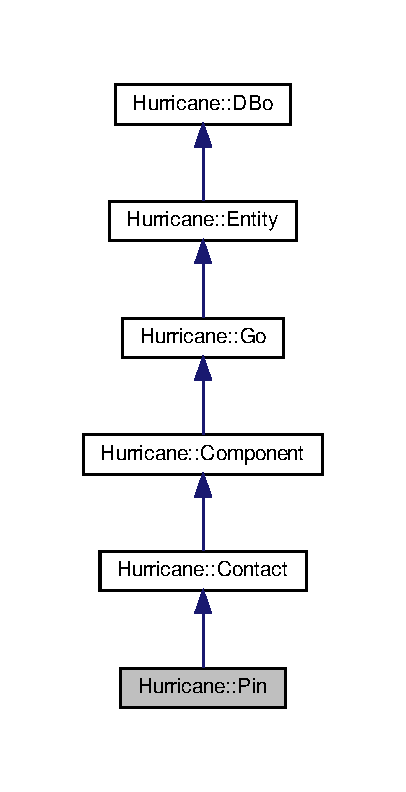
\includegraphics[width=195pt]{classHurricane_1_1Pin__inherit__graph}
\end{center}
\end{figure}
\doxysubsection*{Additional Inherited Members}


\doxysubsection{Detailed Description}
\mbox{\hyperlink{classHurricane_1_1Pin}{Pin}} description ({\bfseries{API}}) 

The documentation for this class was generated from the following file\+:\begin{DoxyCompactItemize}
\item 
Pin.\+h\end{DoxyCompactItemize}

\hypertarget{classHurricane_1_1Instance_1_1PlacementStatus}{}\doxysection{Hurricane\+::Instance\+::Placement\+Status Class Reference}
\label{classHurricane_1_1Instance_1_1PlacementStatus}\index{Hurricane::Instance::PlacementStatus@{Hurricane::Instance::PlacementStatus}}


\mbox{\hyperlink{classHurricane_1_1Instance}{Instance}} Placement Status ({\bfseries{API}})  


\doxysubsection*{Instance Collection}
\begin{DoxyCompactItemize}
\item 
enum \mbox{\hyperlink{classHurricane_1_1Instance_1_1PlacementStatus_af76cc0838783b3eb3a515eb3c3e0f7bf}{Code}} \{ \newline
\mbox{\hyperlink{classHurricane_1_1Instance_1_1PlacementStatus_af76cc0838783b3eb3a515eb3c3e0f7bfa3e19a0a1b3e8c8fd860164df7f935216}{UNPLACED}} =0
, \newline
\mbox{\hyperlink{classHurricane_1_1Instance_1_1PlacementStatus_af76cc0838783b3eb3a515eb3c3e0f7bfaf3589c11ecd7d5de63db24826b74d457}{PLACED}} =1
, \newline
\mbox{\hyperlink{classHurricane_1_1Instance_1_1PlacementStatus_af76cc0838783b3eb3a515eb3c3e0f7bfa47be8a40f04081635fe24485ae7c6bd7}{FIXED}} =2
 \}
\item 
\mbox{\hyperlink{classHurricane_1_1Instance_1_1PlacementStatus_a29d2678343f4b712a9bbbb8f5460ec11}{Placement\+Status}} (const \mbox{\hyperlink{classHurricane_1_1Instance_1_1PlacementStatus_af76cc0838783b3eb3a515eb3c3e0f7bf}{Code}} \&code=\mbox{\hyperlink{classHurricane_1_1Instance_1_1PlacementStatus_af76cc0838783b3eb3a515eb3c3e0f7bfa3e19a0a1b3e8c8fd860164df7f935216}{UNPLACED}})
\item 
\mbox{\hyperlink{classHurricane_1_1Instance_1_1PlacementStatus_a121a628ab6f7a86b99acacc0d874d97b}{Placement\+Status}} (const \mbox{\hyperlink{classHurricane_1_1Instance_1_1PlacementStatus}{Placement\+Status}} \&placementstatus)
\item 
\mbox{\hyperlink{classHurricane_1_1Instance_1_1PlacementStatus_a375d2547ed3e8a127e34b0ee3ca14ad6}{operator const Code \&}} () const
\item 
const \mbox{\hyperlink{classHurricane_1_1Instance_1_1PlacementStatus_af76cc0838783b3eb3a515eb3c3e0f7bf}{Code}} \& \mbox{\hyperlink{classHurricane_1_1Instance_1_1PlacementStatus_aa907067c594076ed8422bf6c949c8731}{get\+Code}} () const
\end{DoxyCompactItemize}


\doxysubsection{Detailed Description}
\mbox{\hyperlink{classHurricane_1_1Instance}{Instance}} Placement Status ({\bfseries{API}}) 

\hypertarget{classHurricane_1_1Instance_1_1PlacementStatus_secInstancePStatus}{}\doxysubsection{Instance Placement Status}\label{classHurricane_1_1Instance_1_1PlacementStatus_secInstancePStatus}
An \mbox{\hyperlink{classHurricane_1_1Instance}{Instance}} can have three kind of placement status\+:
\begin{DoxyItemize}
\item \mbox{\hyperlink{classHurricane_1_1Instance_1_1PlacementStatus_af76cc0838783b3eb3a515eb3c3e0f7bfa3e19a0a1b3e8c8fd860164df7f935216}{Instance\+::\+Placement\+Status\+::\+UNPLACED}} \+: the instance doesn\textquotesingle{}t have a meaningful position. It shouldn\textquotesingle{}t be materialized either. It\textquotesingle{}s position therfore shouldn\textquotesingle{}t be used.
\item \mbox{\hyperlink{classHurricane_1_1Instance_1_1PlacementStatus_af76cc0838783b3eb3a515eb3c3e0f7bfaf3589c11ecd7d5de63db24826b74d457}{Instance\+::\+Placement\+Status\+::\+PLACED}} \+: the instance has be placed manually or by an automated tool. It is movable.
\item \mbox{\hyperlink{classHurricane_1_1Instance_1_1PlacementStatus_af76cc0838783b3eb3a515eb3c3e0f7bfa47be8a40f04081635fe24485ae7c6bd7}{Instance\+::\+Placement\+Status\+::\+FIXED}} \+: the instance is placed and mustn\textquotesingle{}t be moved by automated tools. It can still be moved manually. 
\end{DoxyItemize}

\doxysubsection{Member Enumeration Documentation}
\mbox{\Hypertarget{classHurricane_1_1Instance_1_1PlacementStatus_af76cc0838783b3eb3a515eb3c3e0f7bf}\label{classHurricane_1_1Instance_1_1PlacementStatus_af76cc0838783b3eb3a515eb3c3e0f7bf}} 
\index{Hurricane::Instance::PlacementStatus@{Hurricane::Instance::PlacementStatus}!Code@{Code}}
\index{Code@{Code}!Hurricane::Instance::PlacementStatus@{Hurricane::Instance::PlacementStatus}}
\doxysubsubsection{\texorpdfstring{Code}{Code}}
{\footnotesize\ttfamily enum \mbox{\hyperlink{classHurricane_1_1Instance_1_1PlacementStatus_af76cc0838783b3eb3a515eb3c3e0f7bf}{Hurricane\+::\+Instance\+::\+Placement\+Status\+::\+Code}}}

Describe the various placement status an \mbox{\hyperlink{classHurricane_1_1Instance}{Instance}} can be in. \begin{DoxyEnumFields}{Enumerator}
\raisebox{\heightof{T}}[0pt][0pt]{\index{UNPLACED@{UNPLACED}!Hurricane::Instance::PlacementStatus@{Hurricane::Instance::PlacementStatus}}\index{Hurricane::Instance::PlacementStatus@{Hurricane::Instance::PlacementStatus}!UNPLACED@{UNPLACED}}}\mbox{\Hypertarget{classHurricane_1_1Instance_1_1PlacementStatus_af76cc0838783b3eb3a515eb3c3e0f7bfa3e19a0a1b3e8c8fd860164df7f935216}\label{classHurricane_1_1Instance_1_1PlacementStatus_af76cc0838783b3eb3a515eb3c3e0f7bfa3e19a0a1b3e8c8fd860164df7f935216}} 
UNPLACED&\begin{DoxySeeAlso}{See also}
\mbox{\hyperlink{classHurricane_1_1Instance_1_1PlacementStatus}{Instance\+::\+Placement\+Status}}. 
\end{DoxySeeAlso}
\\
\hline

\raisebox{\heightof{T}}[0pt][0pt]{\index{PLACED@{PLACED}!Hurricane::Instance::PlacementStatus@{Hurricane::Instance::PlacementStatus}}\index{Hurricane::Instance::PlacementStatus@{Hurricane::Instance::PlacementStatus}!PLACED@{PLACED}}}\mbox{\Hypertarget{classHurricane_1_1Instance_1_1PlacementStatus_af76cc0838783b3eb3a515eb3c3e0f7bfaf3589c11ecd7d5de63db24826b74d457}\label{classHurricane_1_1Instance_1_1PlacementStatus_af76cc0838783b3eb3a515eb3c3e0f7bfaf3589c11ecd7d5de63db24826b74d457}} 
PLACED&\begin{DoxySeeAlso}{See also}
\mbox{\hyperlink{classHurricane_1_1Instance_1_1PlacementStatus}{Instance\+::\+Placement\+Status}}. 
\end{DoxySeeAlso}
\\
\hline

\raisebox{\heightof{T}}[0pt][0pt]{\index{FIXED@{FIXED}!Hurricane::Instance::PlacementStatus@{Hurricane::Instance::PlacementStatus}}\index{Hurricane::Instance::PlacementStatus@{Hurricane::Instance::PlacementStatus}!FIXED@{FIXED}}}\mbox{\Hypertarget{classHurricane_1_1Instance_1_1PlacementStatus_af76cc0838783b3eb3a515eb3c3e0f7bfa47be8a40f04081635fe24485ae7c6bd7}\label{classHurricane_1_1Instance_1_1PlacementStatus_af76cc0838783b3eb3a515eb3c3e0f7bfa47be8a40f04081635fe24485ae7c6bd7}} 
FIXED&\begin{DoxySeeAlso}{See also}
\mbox{\hyperlink{classHurricane_1_1Instance_1_1PlacementStatus}{Instance\+::\+Placement\+Status}}. 
\end{DoxySeeAlso}
\\
\hline

\end{DoxyEnumFields}


\doxysubsection{Constructor \& Destructor Documentation}
\mbox{\Hypertarget{classHurricane_1_1Instance_1_1PlacementStatus_a29d2678343f4b712a9bbbb8f5460ec11}\label{classHurricane_1_1Instance_1_1PlacementStatus_a29d2678343f4b712a9bbbb8f5460ec11}} 
\index{Hurricane::Instance::PlacementStatus@{Hurricane::Instance::PlacementStatus}!PlacementStatus@{PlacementStatus}}
\index{PlacementStatus@{PlacementStatus}!Hurricane::Instance::PlacementStatus@{Hurricane::Instance::PlacementStatus}}
\doxysubsubsection{\texorpdfstring{PlacementStatus()}{PlacementStatus()}\hspace{0.1cm}{\footnotesize\ttfamily [1/2]}}
{\footnotesize\ttfamily Hurricane\+::\+Instance\+::\+Placement\+Status\+::\+Placement\+Status (\begin{DoxyParamCaption}\item[{const \mbox{\hyperlink{classHurricane_1_1Instance_1_1PlacementStatus_af76cc0838783b3eb3a515eb3c3e0f7bf}{Code}} \&}]{code = {\ttfamily \mbox{\hyperlink{classHurricane_1_1Instance_1_1PlacementStatus_af76cc0838783b3eb3a515eb3c3e0f7bfa3e19a0a1b3e8c8fd860164df7f935216}{UNPLACED}}} }\end{DoxyParamCaption})}

Constructor. By default the status is unplaced. \mbox{\Hypertarget{classHurricane_1_1Instance_1_1PlacementStatus_a121a628ab6f7a86b99acacc0d874d97b}\label{classHurricane_1_1Instance_1_1PlacementStatus_a121a628ab6f7a86b99acacc0d874d97b}} 
\index{Hurricane::Instance::PlacementStatus@{Hurricane::Instance::PlacementStatus}!PlacementStatus@{PlacementStatus}}
\index{PlacementStatus@{PlacementStatus}!Hurricane::Instance::PlacementStatus@{Hurricane::Instance::PlacementStatus}}
\doxysubsubsection{\texorpdfstring{PlacementStatus()}{PlacementStatus()}\hspace{0.1cm}{\footnotesize\ttfamily [2/2]}}
{\footnotesize\ttfamily Hurricane\+::\+Instance\+::\+Placement\+Status\+::\+Placement\+Status (\begin{DoxyParamCaption}\item[{const \mbox{\hyperlink{classHurricane_1_1Instance_1_1PlacementStatus}{Placement\+Status}} \&}]{placementstatus }\end{DoxyParamCaption})}

Copy Constructor. 

\doxysubsection{Member Function Documentation}
\mbox{\Hypertarget{classHurricane_1_1Instance_1_1PlacementStatus_a375d2547ed3e8a127e34b0ee3ca14ad6}\label{classHurricane_1_1Instance_1_1PlacementStatus_a375d2547ed3e8a127e34b0ee3ca14ad6}} 
\index{Hurricane::Instance::PlacementStatus@{Hurricane::Instance::PlacementStatus}!operator const Code \&@{operator const Code \&}}
\index{operator const Code \&@{operator const Code \&}!Hurricane::Instance::PlacementStatus@{Hurricane::Instance::PlacementStatus}}
\doxysubsubsection{\texorpdfstring{operator const Code \&()}{operator const Code \&()}}
{\footnotesize\ttfamily Hurricane\+::\+Instance\+::\+Placement\+Status\+::operator const \mbox{\hyperlink{classHurricane_1_1Instance_1_1PlacementStatus_af76cc0838783b3eb3a515eb3c3e0f7bf}{Code}} \& (\begin{DoxyParamCaption}{ }\end{DoxyParamCaption}) const\hspace{0.3cm}{\ttfamily [inline]}}

Type converter toward \mbox{\hyperlink{classHurricane_1_1Instance_1_1PlacementStatus_af76cc0838783b3eb3a515eb3c3e0f7bf}{Instance\+::\+Placement\+Status\+::\+Code}} enum. \mbox{\Hypertarget{classHurricane_1_1Instance_1_1PlacementStatus_aa907067c594076ed8422bf6c949c8731}\label{classHurricane_1_1Instance_1_1PlacementStatus_aa907067c594076ed8422bf6c949c8731}} 
\index{Hurricane::Instance::PlacementStatus@{Hurricane::Instance::PlacementStatus}!getCode@{getCode}}
\index{getCode@{getCode}!Hurricane::Instance::PlacementStatus@{Hurricane::Instance::PlacementStatus}}
\doxysubsubsection{\texorpdfstring{getCode()}{getCode()}}
{\footnotesize\ttfamily \mbox{\hyperlink{classHurricane_1_1Instance_1_1PlacementStatus_af76cc0838783b3eb3a515eb3c3e0f7bf}{Instance\+::\+Placement\+Status\+::\+Code}} \& Hurricane\+::\+Instance\+::\+Placement\+Status\+::get\+Code (\begin{DoxyParamCaption}{ }\end{DoxyParamCaption}) const\hspace{0.3cm}{\ttfamily [inline]}}

\begin{DoxyReturn}{Returns}
The status (Code) value. 
\end{DoxyReturn}


The documentation for this class was generated from the following files\+:\begin{DoxyCompactItemize}
\item 
Instance.\+h\item 
Instance.\+dox\end{DoxyCompactItemize}

\hypertarget{classHurricane_1_1Plug}{}\doxysection{Hurricane\+::Plug Class Reference}
\label{classHurricane_1_1Plug}\index{Hurricane::Plug@{Hurricane::Plug}}


\mbox{\hyperlink{classHurricane_1_1Plug}{Plug}} description ({\bfseries{API}})  




Inheritance diagram for Hurricane\+::Plug\+:\nopagebreak
\begin{figure}[H]
\begin{center}
\leavevmode
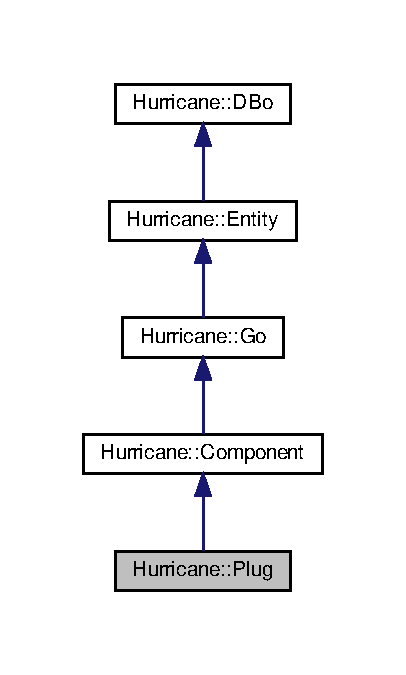
\includegraphics[width=195pt]{classHurricane_1_1Plug__inherit__graph}
\end{center}
\end{figure}
\doxysubsection*{Public Types}
\begin{DoxyCompactItemize}
\item 
typedef \mbox{\hyperlink{classHurricane_1_1Component}{Component}} \mbox{\hyperlink{classHurricane_1_1Plug_a71bee60105cbd9fdc5f0f2e5b793eeca}{Inherit}}
\end{DoxyCompactItemize}
\doxysubsection*{Public Member Functions}
\begin{DoxyCompactItemize}
\item 
\mbox{\hyperlink{classHurricane_1_1Instance}{Instance}} $\ast$ \mbox{\hyperlink{classHurricane_1_1Plug_a6ed1a11f86fbb80afacc9cc31b18a706}{get\+Instance}} () const
\item 
\mbox{\hyperlink{classHurricane_1_1Net}{Net}} $\ast$ \mbox{\hyperlink{classHurricane_1_1Plug_a57860e49d2674dcef6ea27d79c9d2ad8}{get\+Master\+Net}} () const
\item 
bool \mbox{\hyperlink{classHurricane_1_1Plug_a177400e23157885a76c924bf53000957}{is\+Connected}} () const
\item 
void \mbox{\hyperlink{classHurricane_1_1Plug_af5a0448a5cb0c4956f2f1b28f9c87530}{set\+Net}} (\mbox{\hyperlink{classHurricane_1_1Net}{Net}} $\ast$net)
\end{DoxyCompactItemize}
\doxysubsection*{Static Public Member Functions}
\begin{Indent}\textbf{ Plug Collection}\par
\begin{DoxyCompactItemize}
\item 
static \mbox{\hyperlink{namespaceHurricane_ad6b0bd4bdff4c52e6163b9f54e3e5c92}{Plug\+Filter}} \mbox{\hyperlink{classHurricane_1_1Plug_a51bd5d04a337544709950d7cace05f0d}{get\+Is\+Connected\+Filter}} ()
\item 
static \mbox{\hyperlink{namespaceHurricane_ad6b0bd4bdff4c52e6163b9f54e3e5c92}{Plug\+Filter}} \mbox{\hyperlink{classHurricane_1_1Plug_af27b873ed2420329a63ea67dcc243f07}{get\+Is\+Unconnected\+Filter}} ()
\end{DoxyCompactItemize}
\end{Indent}


\doxysubsection{Detailed Description}
\mbox{\hyperlink{classHurricane_1_1Plug}{Plug}} description ({\bfseries{API}}) 

\hypertarget{classHurricane_1_1Plug_secPlugIntro}{}\doxysubsection{Introduction}\label{classHurricane_1_1Plug_secPlugIntro}
A plug can be assimilated to a \char`\"{}logical port instance\char`\"{} \+: it designates both the concerned instance and the net of the model cell instanciated to which it is connected. This net, which must be an external net, will be named {\bfseries{\char`\"{}master                net\char`\"{}}} because it is a net of the instance master cell (notice that this net can be asimilated to a \char`\"{}logical port\char`\"{}).

A plug is unique, that is, for a given instance there is one and only one plug refering to a given master net.

\begin{DoxyParagraph}{Caution\+: When created, an instance creates all plugs corresponding to }
the external nets of its master cell. So, some plugs may exist without being connected. Plugs are the only components which have this characteristic.
\end{DoxyParagraph}
\begin{DoxyRemark}{Remarks}
Plugs being completely managed by the system, you can\textquotesingle{}t define sub-\/types of plugs.
\end{DoxyRemark}
\hypertarget{classHurricane_1_1Plug_secPlugConstructors}{}\doxysubsection{Constructors \& Destructors}\label{classHurricane_1_1Plug_secPlugConstructors}
Plugs being completely managed by the system, there is no constructor nor destructor provided.\hypertarget{classHurricane_1_1Plug_secPlugPredefinedFilters}{}\doxysubsection{Predefined filters}\label{classHurricane_1_1Plug_secPlugPredefinedFilters}
{\bfseries{\mbox{\hyperlink{classHurricane_1_1Plug_a51bd5d04a337544709950d7cace05f0d}{Hurricane\+::\+Plug\+::get\+Is\+Connected\+Filter}}}} {\bfseries{\mbox{\hyperlink{classHurricane_1_1Plug_af27b873ed2420329a63ea67dcc243f07}{Hurricane\+::\+Plug\+::get\+Is\+Unconnected\+Filter}}}} 

\doxysubsection{Member Typedef Documentation}
\mbox{\Hypertarget{classHurricane_1_1Plug_a71bee60105cbd9fdc5f0f2e5b793eeca}\label{classHurricane_1_1Plug_a71bee60105cbd9fdc5f0f2e5b793eeca}} 
\index{Hurricane::Plug@{Hurricane::Plug}!Inherit@{Inherit}}
\index{Inherit@{Inherit}!Hurricane::Plug@{Hurricane::Plug}}
\doxysubsubsection{\texorpdfstring{Inherit}{Inherit}}
{\footnotesize\ttfamily \mbox{\hyperlink{classHurricane_1_1Plug_a71bee60105cbd9fdc5f0f2e5b793eeca}{Hurricane\+::\+Plug\+::\+Inherit}}}

Useful for calling upon methods of the base class without knowing it. 

\doxysubsection{Member Function Documentation}
\mbox{\Hypertarget{classHurricane_1_1Plug_a6ed1a11f86fbb80afacc9cc31b18a706}\label{classHurricane_1_1Plug_a6ed1a11f86fbb80afacc9cc31b18a706}} 
\index{Hurricane::Plug@{Hurricane::Plug}!getInstance@{getInstance}}
\index{getInstance@{getInstance}!Hurricane::Plug@{Hurricane::Plug}}
\doxysubsubsection{\texorpdfstring{getInstance()}{getInstance()}}
{\footnotesize\ttfamily \mbox{\hyperlink{classHurricane_1_1Instance}{Instance}} $\ast$ Hurricane\+::\+Plug\+::get\+Instance (\begin{DoxyParamCaption}{ }\end{DoxyParamCaption}) const\hspace{0.3cm}{\ttfamily [inline]}}

{\bfseries{Returns\+:}} the instance to which belongs the plug. \mbox{\Hypertarget{classHurricane_1_1Plug_a57860e49d2674dcef6ea27d79c9d2ad8}\label{classHurricane_1_1Plug_a57860e49d2674dcef6ea27d79c9d2ad8}} 
\index{Hurricane::Plug@{Hurricane::Plug}!getMasterNet@{getMasterNet}}
\index{getMasterNet@{getMasterNet}!Hurricane::Plug@{Hurricane::Plug}}
\doxysubsubsection{\texorpdfstring{getMasterNet()}{getMasterNet()}}
{\footnotesize\ttfamily \mbox{\hyperlink{classHurricane_1_1Net}{Net}} $\ast$ Hurricane\+::\+Plug\+::get\+Master\+Net (\begin{DoxyParamCaption}{ }\end{DoxyParamCaption}) const\hspace{0.3cm}{\ttfamily [inline]}}

{\bfseries{Returns\+:}} the external net referenced by the plug in the master cell of its instance.

\begin{DoxyRemark}{Remarks}
Don\textquotesingle{}t mistake with \mbox{\hyperlink{classHurricane_1_1Component_a1556ef77d6b89bfc17698d52ebde9791}{get\+Net()}} which returns the net owning the plug (or NULL if is unconnected). 
\end{DoxyRemark}
\mbox{\Hypertarget{classHurricane_1_1Plug_a51bd5d04a337544709950d7cace05f0d}\label{classHurricane_1_1Plug_a51bd5d04a337544709950d7cace05f0d}} 
\index{Hurricane::Plug@{Hurricane::Plug}!getIsConnectedFilter@{getIsConnectedFilter}}
\index{getIsConnectedFilter@{getIsConnectedFilter}!Hurricane::Plug@{Hurricane::Plug}}
\doxysubsubsection{\texorpdfstring{getIsConnectedFilter()}{getIsConnectedFilter()}}
{\footnotesize\ttfamily \mbox{\hyperlink{namespaceHurricane_ad6b0bd4bdff4c52e6163b9f54e3e5c92}{Plug\+Filter}} Hurricane\+::\+Plug\+::get\+Is\+Connected\+Filter (\begin{DoxyParamCaption}{ }\end{DoxyParamCaption})\hspace{0.3cm}{\ttfamily [static]}}

{\bfseries{Returns\+:}} a filter for selecting only connected plugs. \mbox{\Hypertarget{classHurricane_1_1Plug_af27b873ed2420329a63ea67dcc243f07}\label{classHurricane_1_1Plug_af27b873ed2420329a63ea67dcc243f07}} 
\index{Hurricane::Plug@{Hurricane::Plug}!getIsUnconnectedFilter@{getIsUnconnectedFilter}}
\index{getIsUnconnectedFilter@{getIsUnconnectedFilter}!Hurricane::Plug@{Hurricane::Plug}}
\doxysubsubsection{\texorpdfstring{getIsUnconnectedFilter()}{getIsUnconnectedFilter()}}
{\footnotesize\ttfamily \mbox{\hyperlink{namespaceHurricane_ad6b0bd4bdff4c52e6163b9f54e3e5c92}{Plug\+Filter}} Hurricane\+::\+Plug\+::get\+Is\+Unconnected\+Filter (\begin{DoxyParamCaption}{ }\end{DoxyParamCaption})\hspace{0.3cm}{\ttfamily [static]}}

{\bfseries{Returns\+:}} a filter for selecting only unconnected plugs. \mbox{\Hypertarget{classHurricane_1_1Plug_a177400e23157885a76c924bf53000957}\label{classHurricane_1_1Plug_a177400e23157885a76c924bf53000957}} 
\index{Hurricane::Plug@{Hurricane::Plug}!isConnected@{isConnected}}
\index{isConnected@{isConnected}!Hurricane::Plug@{Hurricane::Plug}}
\doxysubsubsection{\texorpdfstring{isConnected()}{isConnected()}}
{\footnotesize\ttfamily bool Hurricane\+::\+Plug\+::is\+Connected (\begin{DoxyParamCaption}{ }\end{DoxyParamCaption}) const\hspace{0.3cm}{\ttfamily [inline]}}

{\bfseries{Returns\+:}} {\bfseries{true}} if the plug is connected, else {\bfseries{false}}.

\begin{DoxyRemark}{Remarks}
A plug is connected if the call upon {\bfseries{\mbox{\hyperlink{classHurricane_1_1Component_a1556ef77d6b89bfc17698d52ebde9791}{get\+Net()}}}} doesn\textquotesingle{}t return NULL. 
\end{DoxyRemark}


References Hurricane\+::\+Component\+::get\+Net().

\mbox{\Hypertarget{classHurricane_1_1Plug_af5a0448a5cb0c4956f2f1b28f9c87530}\label{classHurricane_1_1Plug_af5a0448a5cb0c4956f2f1b28f9c87530}} 
\index{Hurricane::Plug@{Hurricane::Plug}!setNet@{setNet}}
\index{setNet@{setNet}!Hurricane::Plug@{Hurricane::Plug}}
\doxysubsubsection{\texorpdfstring{setNet()}{setNet()}}
{\footnotesize\ttfamily void Hurricane\+::\+Plug\+::set\+Net (\begin{DoxyParamCaption}\item[{\mbox{\hyperlink{classHurricane_1_1Net}{Net}} $\ast$}]{net }\end{DoxyParamCaption})}

This method allows to connect or change the net of a plug.

\begin{DoxyParagraph}{Caution\+: An exception is thrown if the net owner cell differs from the }
plug owner cell, or if there are components (contact, segments, ...) currently anchored on the plug.
\end{DoxyParagraph}
\begin{DoxyRemark}{Remarks}
The properties attached to this plug and its occurences are left unchanged. 
\end{DoxyRemark}


The documentation for this class was generated from the following files\+:\begin{DoxyCompactItemize}
\item 
Plug.\+h\item 
Plug.\+dox\end{DoxyCompactItemize}

\hypertarget{classHurricane_1_1Point}{}\section{Hurricane\+:\+:Point Class Reference}
\label{classHurricane_1_1Point}\index{Hurricane\+::\+Point@{Hurricane\+::\+Point}}


\mbox{\hyperlink{classHurricane_1_1Point}{Point}} description ({\bfseries A\+PI})  


\subsection*{Public Member Functions}
\begin{DoxyCompactItemize}
\item 
\mbox{\hyperlink{classHurricane_1_1Point_a54c8ad2b1f3005ac1564c0fd7d5ef5b7}{Point}} ()
\item 
\mbox{\hyperlink{classHurricane_1_1Point_a871672d833661cc79101d1e43d4d8325}{Point}} (const \mbox{\hyperlink{group__DbUGroup_ga4fbfa3e8c89347af76c9628ea06c4146}{Db\+U\+::\+Unit}} \&x, const \mbox{\hyperlink{group__DbUGroup_ga4fbfa3e8c89347af76c9628ea06c4146}{Db\+U\+::\+Unit}} \&y)
\item 
\mbox{\hyperlink{classHurricane_1_1Point_a8840ca5f42bec6203058911ea0ba6cb9}{Point}} (const \mbox{\hyperlink{classHurricane_1_1Point}{Point}} \&point)
\item 
\mbox{\hyperlink{classHurricane_1_1Point}{Point}} \& \mbox{\hyperlink{classHurricane_1_1Point_ae3e33361927744a483d97cb7d182a1d6}{operator=}} (const \mbox{\hyperlink{classHurricane_1_1Point}{Point}} \&point)
\item 
bool \mbox{\hyperlink{classHurricane_1_1Point_a2aeb5fe96fbe9324dcbc90d41ad70fb9}{operator==}} (const \mbox{\hyperlink{classHurricane_1_1Point}{Point}} \&point) const
\item 
bool \mbox{\hyperlink{classHurricane_1_1Point_ac6a0b7107f04913b78f96afa69e68d86}{operator!=}} (const \mbox{\hyperlink{classHurricane_1_1Point}{Point}} \&point) const
\item 
void \mbox{\hyperlink{classHurricane_1_1Point_adebab98c82f881b1d2e1e7680a907830}{setX}} (\mbox{\hyperlink{group__DbUGroup_ga4fbfa3e8c89347af76c9628ea06c4146}{Db\+U\+::\+Unit}} x)
\item 
void \mbox{\hyperlink{classHurricane_1_1Point_a14a51f177d298ccccb25066c0298a268}{setY}} (\mbox{\hyperlink{group__DbUGroup_ga4fbfa3e8c89347af76c9628ea06c4146}{Db\+U\+::\+Unit}} y)
\item 
\mbox{\hyperlink{classHurricane_1_1Point}{Point}} \& \mbox{\hyperlink{classHurricane_1_1Point_a86d908d60346bc15f1af4e96eddbdb19}{translate}} (const \mbox{\hyperlink{group__DbUGroup_ga4fbfa3e8c89347af76c9628ea06c4146}{Db\+U\+::\+Unit}} \&dx, const \mbox{\hyperlink{group__DbUGroup_ga4fbfa3e8c89347af76c9628ea06c4146}{Db\+U\+::\+Unit}} \&dy)
\end{DoxyCompactItemize}


\subsection{Detailed Description}
\mbox{\hyperlink{classHurricane_1_1Point}{Point}} description ({\bfseries A\+PI}) 

\subsection{Constructor \& Destructor Documentation}
\mbox{\Hypertarget{classHurricane_1_1Point_a54c8ad2b1f3005ac1564c0fd7d5ef5b7}\label{classHurricane_1_1Point_a54c8ad2b1f3005ac1564c0fd7d5ef5b7}} 
\index{Hurricane\+::\+Point@{Hurricane\+::\+Point}!Point@{Point}}
\index{Point@{Point}!Hurricane\+::\+Point@{Hurricane\+::\+Point}}
\subsubsection{\texorpdfstring{Point()}{Point()}\hspace{0.1cm}{\footnotesize\ttfamily [1/3]}}
{\footnotesize\ttfamily Hurricane\+::\+Point\+::\+Point (\begin{DoxyParamCaption}{ }\end{DoxyParamCaption})}

Default constructor. \mbox{\Hypertarget{classHurricane_1_1Point_a871672d833661cc79101d1e43d4d8325}\label{classHurricane_1_1Point_a871672d833661cc79101d1e43d4d8325}} 
\index{Hurricane\+::\+Point@{Hurricane\+::\+Point}!Point@{Point}}
\index{Point@{Point}!Hurricane\+::\+Point@{Hurricane\+::\+Point}}
\subsubsection{\texorpdfstring{Point()}{Point()}\hspace{0.1cm}{\footnotesize\ttfamily [2/3]}}
{\footnotesize\ttfamily Hurricane\+::\+Point\+::\+Point (\begin{DoxyParamCaption}\item[{const \mbox{\hyperlink{group__DbUGroup_ga4fbfa3e8c89347af76c9628ea06c4146}{Db\+U\+::\+Unit}} \&}]{x,  }\item[{const \mbox{\hyperlink{group__DbUGroup_ga4fbfa3e8c89347af76c9628ea06c4146}{Db\+U\+::\+Unit}} \&}]{y }\end{DoxyParamCaption})}

Creates the point defined by x and y coordinates. \mbox{\Hypertarget{classHurricane_1_1Point_a8840ca5f42bec6203058911ea0ba6cb9}\label{classHurricane_1_1Point_a8840ca5f42bec6203058911ea0ba6cb9}} 
\index{Hurricane\+::\+Point@{Hurricane\+::\+Point}!Point@{Point}}
\index{Point@{Point}!Hurricane\+::\+Point@{Hurricane\+::\+Point}}
\subsubsection{\texorpdfstring{Point()}{Point()}\hspace{0.1cm}{\footnotesize\ttfamily [3/3]}}
{\footnotesize\ttfamily Hurricane\+::\+Point\+::\+Point (\begin{DoxyParamCaption}\item[{const \mbox{\hyperlink{classHurricane_1_1Point}{Point}} \&}]{point }\end{DoxyParamCaption})}

Copy constructor. 

\subsection{Member Function Documentation}
\mbox{\Hypertarget{classHurricane_1_1Point_ae3e33361927744a483d97cb7d182a1d6}\label{classHurricane_1_1Point_ae3e33361927744a483d97cb7d182a1d6}} 
\index{Hurricane\+::\+Point@{Hurricane\+::\+Point}!operator=@{operator=}}
\index{operator=@{operator=}!Hurricane\+::\+Point@{Hurricane\+::\+Point}}
\subsubsection{\texorpdfstring{operator=()}{operator=()}}
{\footnotesize\ttfamily \mbox{\hyperlink{classHurricane_1_1Point}{Point}} \& Hurricane\+::\+Point\+::operator= (\begin{DoxyParamCaption}\item[{const \mbox{\hyperlink{classHurricane_1_1Point}{Point}} \&}]{point }\end{DoxyParamCaption})}

Assignment operator. \mbox{\Hypertarget{classHurricane_1_1Point_a2aeb5fe96fbe9324dcbc90d41ad70fb9}\label{classHurricane_1_1Point_a2aeb5fe96fbe9324dcbc90d41ad70fb9}} 
\index{Hurricane\+::\+Point@{Hurricane\+::\+Point}!operator==@{operator==}}
\index{operator==@{operator==}!Hurricane\+::\+Point@{Hurricane\+::\+Point}}
\subsubsection{\texorpdfstring{operator==()}{operator==()}}
{\footnotesize\ttfamily bool Hurricane\+::\+Point\+::operator== (\begin{DoxyParamCaption}\item[{const \mbox{\hyperlink{classHurricane_1_1Point}{Point}} \&}]{point }\end{DoxyParamCaption}) const}

Equality operator. \mbox{\Hypertarget{classHurricane_1_1Point_ac6a0b7107f04913b78f96afa69e68d86}\label{classHurricane_1_1Point_ac6a0b7107f04913b78f96afa69e68d86}} 
\index{Hurricane\+::\+Point@{Hurricane\+::\+Point}!operator"!=@{operator"!=}}
\index{operator"!=@{operator"!=}!Hurricane\+::\+Point@{Hurricane\+::\+Point}}
\subsubsection{\texorpdfstring{operator"!=()}{operator!=()}}
{\footnotesize\ttfamily bool Hurricane\+::\+Point\+::operator!= (\begin{DoxyParamCaption}\item[{const \mbox{\hyperlink{classHurricane_1_1Point}{Point}} \&}]{point }\end{DoxyParamCaption}) const}

Difference operator. \mbox{\Hypertarget{classHurricane_1_1Point_adebab98c82f881b1d2e1e7680a907830}\label{classHurricane_1_1Point_adebab98c82f881b1d2e1e7680a907830}} 
\index{Hurricane\+::\+Point@{Hurricane\+::\+Point}!setX@{setX}}
\index{setX@{setX}!Hurricane\+::\+Point@{Hurricane\+::\+Point}}
\subsubsection{\texorpdfstring{set\+X()}{setX()}}
{\footnotesize\ttfamily void Hurricane\+::\+Point\+::setX (\begin{DoxyParamCaption}\item[{\mbox{\hyperlink{group__DbUGroup_ga4fbfa3e8c89347af76c9628ea06c4146}{Db\+U\+::\+Unit}}}]{x }\end{DoxyParamCaption})\hspace{0.3cm}{\ttfamily [inline]}}

Modifies point abscissa. \mbox{\Hypertarget{classHurricane_1_1Point_a14a51f177d298ccccb25066c0298a268}\label{classHurricane_1_1Point_a14a51f177d298ccccb25066c0298a268}} 
\index{Hurricane\+::\+Point@{Hurricane\+::\+Point}!setY@{setY}}
\index{setY@{setY}!Hurricane\+::\+Point@{Hurricane\+::\+Point}}
\subsubsection{\texorpdfstring{set\+Y()}{setY()}}
{\footnotesize\ttfamily void Hurricane\+::\+Point\+::setY (\begin{DoxyParamCaption}\item[{\mbox{\hyperlink{group__DbUGroup_ga4fbfa3e8c89347af76c9628ea06c4146}{Db\+U\+::\+Unit}}}]{y }\end{DoxyParamCaption})\hspace{0.3cm}{\ttfamily [inline]}}

Modifies point ordinate. \mbox{\Hypertarget{classHurricane_1_1Point_a86d908d60346bc15f1af4e96eddbdb19}\label{classHurricane_1_1Point_a86d908d60346bc15f1af4e96eddbdb19}} 
\index{Hurricane\+::\+Point@{Hurricane\+::\+Point}!translate@{translate}}
\index{translate@{translate}!Hurricane\+::\+Point@{Hurricane\+::\+Point}}
\subsubsection{\texorpdfstring{translate()}{translate()}}
{\footnotesize\ttfamily \mbox{\hyperlink{classHurricane_1_1Point}{Point}} \& Hurricane\+::\+Point\+::translate (\begin{DoxyParamCaption}\item[{const \mbox{\hyperlink{group__DbUGroup_ga4fbfa3e8c89347af76c9628ea06c4146}{Db\+U\+::\+Unit}} \&}]{dx,  }\item[{const \mbox{\hyperlink{group__DbUGroup_ga4fbfa3e8c89347af76c9628ea06c4146}{Db\+U\+::\+Unit}} \&}]{dy }\end{DoxyParamCaption})}

Translates the point of dx and dy. 

The documentation for this class was generated from the following files\+:\begin{DoxyCompactItemize}
\item 
Point.\+h\item 
Point.\+dox\end{DoxyCompactItemize}

\hypertarget{classHurricane_1_1Polygon}{}\doxysection{Hurricane\+::Polygon Class Reference}
\label{classHurricane_1_1Polygon}\index{Hurricane::Polygon@{Hurricane::Polygon}}


\mbox{\hyperlink{classHurricane_1_1Polygon}{Polygon}} description ({\bfseries{API}})  




Inheritance diagram for Hurricane\+::Polygon\+:\nopagebreak
\begin{figure}[H]
\begin{center}
\leavevmode
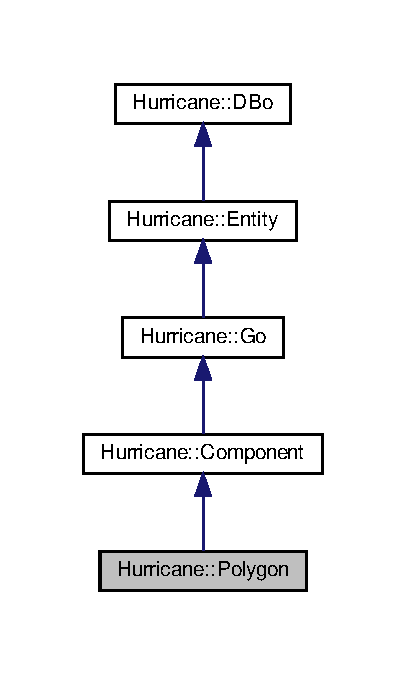
\includegraphics[width=195pt]{classHurricane_1_1Polygon__inherit__graph}
\end{center}
\end{figure}
\doxysubsection*{Public Types}
\begin{DoxyCompactItemize}
\item 
typedef \mbox{\hyperlink{classHurricane_1_1Component}{Component}} \mbox{\hyperlink{classHurricane_1_1Polygon_adac4dcd1480b81e7778775540b95f81c}{Super}}
\end{DoxyCompactItemize}
\doxysubsection*{Static Public Member Functions}
\begin{DoxyCompactItemize}
\item 
static \mbox{\hyperlink{classHurricane_1_1Polygon}{Polygon}} $\ast$ \mbox{\hyperlink{classHurricane_1_1Polygon_ac248679558ff51bf509b28050027b7da}{create}} (\mbox{\hyperlink{classHurricane_1_1Net}{Net}} $\ast$, const \mbox{\hyperlink{classHurricane_1_1Layer}{Layer}} $\ast$, const std\+::vector$<$ \mbox{\hyperlink{classHurricane_1_1Point}{Point}} $>$ \&)
\end{DoxyCompactItemize}
\doxysubsection*{Additional Inherited Members}


\doxysubsection{Detailed Description}
\mbox{\hyperlink{classHurricane_1_1Polygon}{Polygon}} description ({\bfseries{API}}) 

\hypertarget{classHurricane_1_1Polygon_secPolygonIntro}{}\doxysubsection{Introduction}\label{classHurricane_1_1Polygon_secPolygonIntro}
\mbox{\hyperlink{classHurricane_1_1Polygon}{Polygon}} should be used to create huge convex and manhattanized polygons. Manhattanization is done so the real geometric shape is completly included in it. The memory representation has been optimized for very large shape (compare to the foundry grid) and is inefficient for small ones.

The minimal step length for the manhattanisation is set up with Db\+U\+::set\+Polygon\+Step().

\begin{DoxyWarning}{Warning}
\mbox{\hyperlink{classHurricane_1_1Polygon}{Polygon}} objects {\bfseries{cannot}} be exported in symbolic layout. 
\end{DoxyWarning}


\doxysubsection{Member Typedef Documentation}
\mbox{\Hypertarget{classHurricane_1_1Polygon_adac4dcd1480b81e7778775540b95f81c}\label{classHurricane_1_1Polygon_adac4dcd1480b81e7778775540b95f81c}} 
\index{Hurricane::Polygon@{Hurricane::Polygon}!Super@{Super}}
\index{Super@{Super}!Hurricane::Polygon@{Hurricane::Polygon}}
\doxysubsubsection{\texorpdfstring{Super}{Super}}
{\footnotesize\ttfamily \mbox{\hyperlink{classHurricane_1_1Polygon_adac4dcd1480b81e7778775540b95f81c}{Hurricane\+::\+Polygon\+::\+Super}}}

Useful for calling upon methods of the base class without knowing it. 

\doxysubsection{Member Function Documentation}
\mbox{\Hypertarget{classHurricane_1_1Polygon_ac248679558ff51bf509b28050027b7da}\label{classHurricane_1_1Polygon_ac248679558ff51bf509b28050027b7da}} 
\index{Hurricane::Polygon@{Hurricane::Polygon}!create@{create}}
\index{create@{create}!Hurricane::Polygon@{Hurricane::Polygon}}
\doxysubsubsection{\texorpdfstring{create()}{create()}}
{\footnotesize\ttfamily \mbox{\hyperlink{classHurricane_1_1Polygon}{Polygon}} $\ast$ Hurricane\+::\+Polygon\+::create (\begin{DoxyParamCaption}\item[{\mbox{\hyperlink{classHurricane_1_1Net}{Net}} $\ast$}]{net,  }\item[{const \mbox{\hyperlink{classHurricane_1_1Layer}{Layer}} $\ast$}]{layer,  }\item[{const std\+::vector$<$ \mbox{\hyperlink{classHurricane_1_1Point}{Point}} $>$ \&}]{points }\end{DoxyParamCaption})\hspace{0.3cm}{\ttfamily [static]}}

Create a polygon of {\ttfamily layer} in {\ttfamily net}. {\ttfamily points} define the vertexes. 

The documentation for this class was generated from the following files\+:\begin{DoxyCompactItemize}
\item 
Polygon.\+h\item 
Polygon.\+dox\end{DoxyCompactItemize}

\hypertarget{classHurricane_1_1PrivateProperty}{}\doxysection{Hurricane\+::Private\+Property Class Reference}
\label{classHurricane_1_1PrivateProperty}\index{Hurricane::PrivateProperty@{Hurricane::PrivateProperty}}


\mbox{\hyperlink{classHurricane_1_1PrivateProperty}{Private\+Property}} description ({\bfseries{API}})  




Inheritance diagram for Hurricane\+::Private\+Property\+:\nopagebreak
\begin{figure}[H]
\begin{center}
\leavevmode
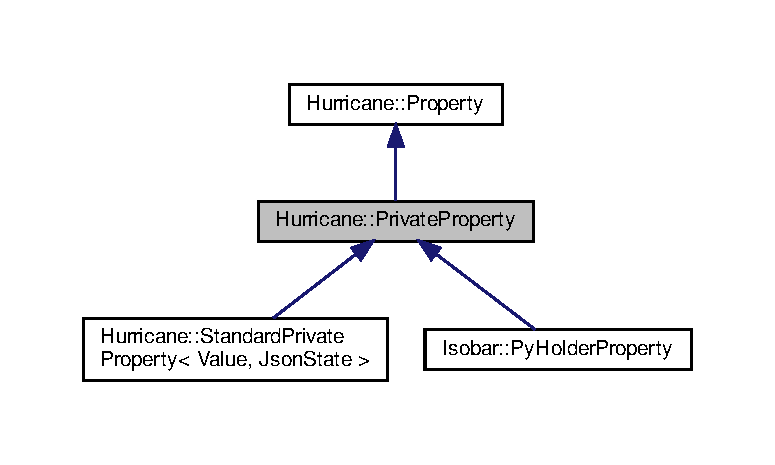
\includegraphics[width=350pt]{classHurricane_1_1PrivateProperty__inherit__graph}
\end{center}
\end{figure}
\doxysubsection*{Public Member Functions}
\begin{DoxyCompactItemize}
\item 
\mbox{\hyperlink{classHurricane_1_1DBo}{DBo}} $\ast$ \mbox{\hyperlink{classHurricane_1_1PrivateProperty_a070ea464f4859734163b12a134e2d8f2}{get\+Owner}} () const
\end{DoxyCompactItemize}


\doxysubsection{Detailed Description}
\mbox{\hyperlink{classHurricane_1_1PrivateProperty}{Private\+Property}} description ({\bfseries{API}}) 

\hypertarget{classHurricane_1_1PrivateProperty_secPrivatePropertyIntro}{}\doxysubsection{Introduction}\label{classHurricane_1_1PrivateProperty_secPrivatePropertyIntro}
Private properties are owned by only one data base object.

When a new property is created, it is not yet assigned to any particular object. It becomes effectively the property of an object after the call {\bfseries{dbo-\/$>$put(property)}}. The property then receives a message {\bfseries{on\+Captured\+By}} whose argument is the additional owner. From that time onwards, this object becomes partially responsible of the future of the property.

{\bfseries{What can happen then ?}}

If the property is destroyed \+: The property, being private, informs its owner (if any) of its deletion which detaches it from its property list (if the object is a quark and if this was the last property owned, it has no more reason to exist and automatically deletes itself).

If a property of same name already exist \+: Two properties with the same name can\textquotesingle{}t cohabit, the older one is released by the object which receives the message {\bfseries{on\+Released\+By}} from that old property and proceeds as required according to the type of property.

If the property changes of owner \+: This one is first captured by the new owner and the released by the older owner (the reason why messages are called upon in this order will be explained later).

If the property owner is destroyed \+: All properties owned by the object are then released. The future of each of those properties is fully driven by their respective messages {\bfseries{on\+Released\+By}}. 

\doxysubsection{Member Function Documentation}
\mbox{\Hypertarget{classHurricane_1_1PrivateProperty_a070ea464f4859734163b12a134e2d8f2}\label{classHurricane_1_1PrivateProperty_a070ea464f4859734163b12a134e2d8f2}} 
\index{Hurricane::PrivateProperty@{Hurricane::PrivateProperty}!getOwner@{getOwner}}
\index{getOwner@{getOwner}!Hurricane::PrivateProperty@{Hurricane::PrivateProperty}}
\doxysubsubsection{\texorpdfstring{getOwner()}{getOwner()}}
{\footnotesize\ttfamily \mbox{\hyperlink{classHurricane_1_1DBo}{DBo}} $\ast$ Hurricane\+::\+Private\+Property\+::get\+Owner (\begin{DoxyParamCaption}{ }\end{DoxyParamCaption}) const\hspace{0.3cm}{\ttfamily [inline]}}

\hypertarget{classHurricane_1_1PrivateProperty_secPrivatePropertyDestruction}{}\doxysubsection{Destruction}\label{classHurricane_1_1PrivateProperty_secPrivatePropertyDestruction}
The property has an owner, this one is informed of the property deletion and detaches it from its property list. If the object is a quark and if this was the last property owned it automatically deletes itself.

\begin{DoxyRemark}{Remarks}
Once the property is attached to an object this one becomes responsible of its automatic destruction. When a property changes its owner, the old owner delegates this task to the new one. On the other hand, a property which has never been attached to an owner will never be deleted automatically.
\end{DoxyRemark}
{\bfseries{Returns\+:}} the current owner of the property (or NULL if at not been assigned yet). 

The documentation for this class was generated from the following files\+:\begin{DoxyCompactItemize}
\item 
Property.\+h\item 
Private\+Property.\+dox\end{DoxyCompactItemize}

\hypertarget{classHurricane_1_1Property}{}\doxysection{Hurricane\+::Property Class Reference}
\label{classHurricane_1_1Property}\index{Hurricane::Property@{Hurricane::Property}}


\mbox{\hyperlink{classHurricane_1_1Property}{Property}} description ({\bfseries{API}})  




Inheritance diagram for Hurricane\+::Property\+:\nopagebreak
\begin{figure}[H]
\begin{center}
\leavevmode
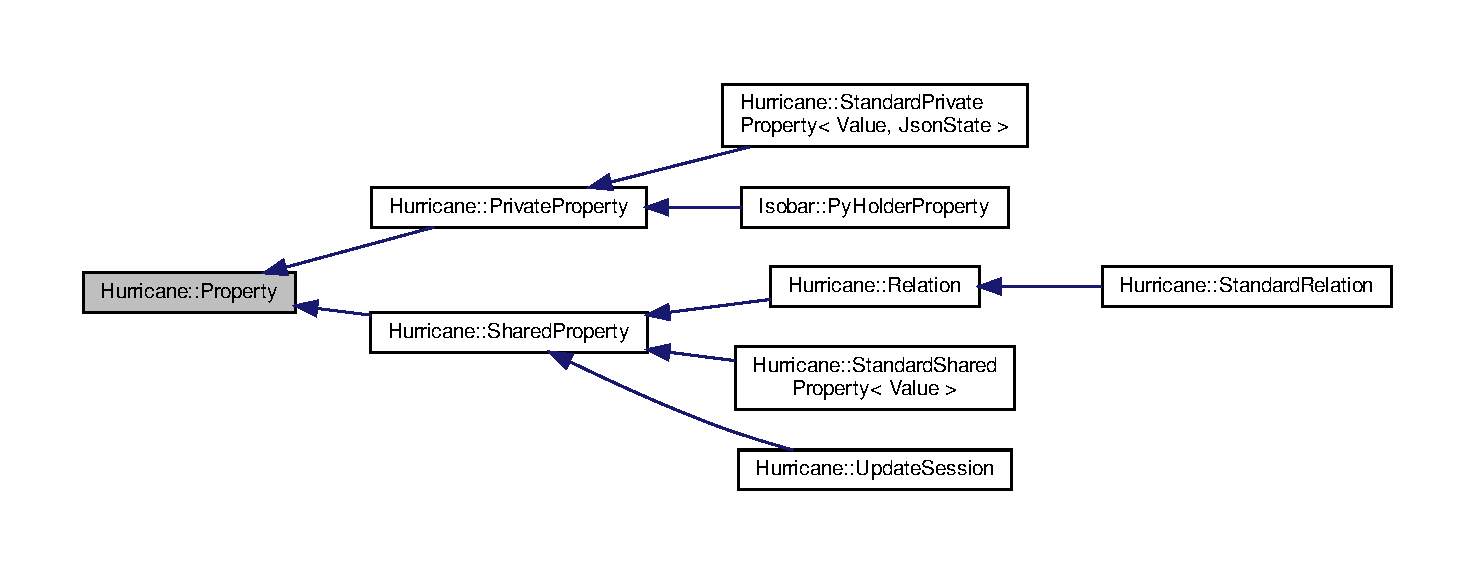
\includegraphics[width=350pt]{classHurricane_1_1Property__inherit__graph}
\end{center}
\end{figure}
\doxysubsection*{Public Member Functions}
\begin{DoxyCompactItemize}
\item 
virtual \mbox{\hyperlink{classHurricane_1_1Name}{Name}} \mbox{\hyperlink{classHurricane_1_1Property_a2759e2003c15d417b925092bc253ddd1}{get\+Name}} () const =0
\item 
virtual void \mbox{\hyperlink{classHurricane_1_1Property_ac7b936414d9d85bb6509100b5dd6a667}{on\+Captured\+By}} (\mbox{\hyperlink{classHurricane_1_1DBo}{DBo}} $\ast$owner)=0
\item 
virtual void \mbox{\hyperlink{classHurricane_1_1Property_a0ea7ee2089f1463c0c16e30313b54083}{on\+Released\+By}} (\mbox{\hyperlink{classHurricane_1_1DBo}{DBo}} $\ast$owner)=0
\end{DoxyCompactItemize}
\begin{Indent}\textbf{ Property Collection}\par
\begin{DoxyCompactItemize}
\item 
virtual void \mbox{\hyperlink{classHurricane_1_1Property_ab60362699e6c6ea35ace45dbd1075a2f}{destroy}} ()
\end{DoxyCompactItemize}
\end{Indent}


\doxysubsection{Detailed Description}
\mbox{\hyperlink{classHurricane_1_1Property}{Property}} description ({\bfseries{API}}) 

\hypertarget{classHurricane_1_1Property_secPropertyIntro}{}\doxysubsection{Introduction}\label{classHurricane_1_1Property_secPropertyIntro}
Properties can be attached to the data base objects. Those properties must have a name in order to access them unambiguously. Of course only one property of a given name can be attached to an object.

In a first step we define two great categories of properties \+: the private properties which can be attached to only one object and the shared properties which can be attached to a large number of objects.

We will detail separately their respective behaviour, but we ensure that the management of each of those two property categories is absolutely secure. That is, on one side you can destroy explicitely a property (and the objects will be notified) and on the other side the properties will be automatically destroyed when no more object reference them.

\begin{DoxyRemark}{Remarks}
By overloading some messages, as we will see later, it is possible to set up different behaviours (like avoid the automatic delete).
\end{DoxyRemark}
\hypertarget{classHurricane_1_1Property_secPropertyTheQuarks}{}\doxysubsection{The Quarks}\label{classHurricane_1_1Property_secPropertyTheQuarks}
As we shall see, the occurences are very simple objects which are used to designate some entity of the virtually unfolded hierarchy. Indeed, those occurences, which are built and deleted very quickly, are very volatile objects to which obvioulsy we can\textquotesingle{}t attach properties directly.

But the interest of occurences is precisely to be able to attach them properties. In order to be able to do that, properties must be stored in a secure place where we could find them when needed. The quarks are here for that purpose \+: they are subtypes of data base object and therefore can store the properties attached to occurences.

\begin{DoxyParagraph}{Important\+:\textbackslash{}n only one quark is attached to all occurences which refer the }
same entity of the virtually unfolded hierarchy. This means that a property placed on an occurence can be read by any other occurence which refers the same entity of the virtually unfolded hierarchy.
\end{DoxyParagraph}
\begin{DoxyRemark}{Remarks}
Those quarks are also volatile objects because their only reason to exist is that at least one property is attached to them.
\end{DoxyRemark}
\hypertarget{classHurricane_1_1Property_secPropertyHowThatWorks}{}\doxysubsection{How that works}\label{classHurricane_1_1Property_secPropertyHowThatWorks}
We will detail the way properties are managed by analysing more precisely what happens at the level of property access functions both for data base objects and for occurences.

{\bfseries{Accessing a property by its name}} 
\begin{DoxyCode}{0}
\DoxyCodeLine{Property* \mbox{\hyperlink{classHurricane_1_1DBo_a599f61978df51d1d4c351f6cbd02488d}{DBo::getProperty}}(\textcolor{keyword}{const} Name\& name) \textcolor{keyword}{const};}

\end{DoxyCode}
 This member function returns the property of name {\ttfamily $<$name$>$} if there is one attached to the object, else NULL. 
\begin{DoxyCode}{0}
\DoxyCodeLine{Property* \mbox{\hyperlink{classHurricane_1_1Occurrence_ab2b36b219037a2310f6527a35a9a266f}{Occurrence::getProperty}}(\textcolor{keyword}{const} Name\& name) \textcolor{keyword}{const};}

\end{DoxyCode}
 This function searches in a first time the quark representing the occurence.

If the quark doesn\textquotesingle{}t exist, this means there is no property attached to that occurence, then the function returns NULL.

If the quark does exist, the function returns the property of name {\ttfamily $<$name$>$} attached to the quark, if any, by calling the previous function (because quarks are data base objects).

{\bfseries{Accessing the set of all properties}} 
\begin{DoxyCode}{0}
\DoxyCodeLine{\mbox{\hyperlink{namespaceHurricane_afd7bca6dad4be54b7c03b0463e6c0004}{Properties}}  \mbox{\hyperlink{classHurricane_1_1DBo_aec46894a10e83abb54c495dc4d90f2d3}{DBo::getProperties}}() \textcolor{keyword}{const};}

\end{DoxyCode}
 Return the collection of properties attached to the object (possibly empty). 
\begin{DoxyCode}{0}
\DoxyCodeLine{\mbox{\hyperlink{namespaceHurricane_afd7bca6dad4be54b7c03b0463e6c0004}{Properties}}  \mbox{\hyperlink{classHurricane_1_1Occurrence_acbf59d6c01804e01f66d076c149abb49}{Occurrence::getProperties}}() \textcolor{keyword}{const};}

\end{DoxyCode}
 This function searches in a first time the quark representing the occurence.

If the quark doesn\textquotesingle{}t exist, this means there is no property attached to that occurence, then the function returns an empty property collection.

If the quark does exist, the function returns the property collection attached to the quark, by calling the previous function (the returned collection is inevitably non empty, else the quark would not exist).

{\bfseries{Does the object have properties ?}} 
\begin{DoxyCode}{0}
\DoxyCodeLine{\textcolor{keywordtype}{bool} \mbox{\hyperlink{classHurricane_1_1DBo_a1563f094565030c77592ed82f9a9989b}{DBo::hasProperty}}() \textcolor{keyword}{const};}

\end{DoxyCode}
 Return {\bfseries{true}} if the object owns at least a property, else {\bfseries{false}}. 
\begin{DoxyCode}{0}
\DoxyCodeLine{\textcolor{keywordtype}{bool} \mbox{\hyperlink{classHurricane_1_1Occurrence_a0c1c6cfdf47f33166d108e2311d74e48}{Occurrence::hasProperty}}() \textcolor{keyword}{const};}

\end{DoxyCode}
 This function searches the quark representing the occurence.

If the quark does exist it means there is at least a property assigned to it and the function returns {\bfseries{true}}, else it returns {\bfseries{false}}.

{\bfseries{Adding a property \+: things becomes a little harder}} 
\begin{DoxyCode}{0}
\DoxyCodeLine{\textcolor{keywordtype}{void} \mbox{\hyperlink{classHurricane_1_1DBo_a8979674f11507cb4c7c5251b41ed72d5}{DBo::put}}(Property* property);}

\end{DoxyCode}
 Adds the property {\ttfamily $<$property$>$} to the set of properties of the object. 
\begin{DoxyCode}{0}
\DoxyCodeLine{\textcolor{keywordtype}{void} \mbox{\hyperlink{classHurricane_1_1Occurrence_aaea0bdc4f5bb4012eb52f3abe20525be}{Occurrence::put}}(Property* property);}

\end{DoxyCode}
 This function searches the quark representing the occurence.

If the quark doesn\textquotesingle{}t exist it is automatically created in order to attach this first property.

once the quark has been got or created, we can add the property with the previous function.

Two important things might happen then \+: The property is already owned by an other object (may be a quark) and that property is not a shared one {\bfseries{and/or}} the object owns already a property with the same name.

Therefore it may happen, within this step, that adding a property to an object leads to the deletion of an other property on that object {\bfseries{(name unicity)}} or on an other object {\bfseries{(unicity of owner for a private property)}}.

Which behaviour should we have in such conditions ? Shall we destroy the property which has been detached ? There is no unique behaviour which matches all needs. In order to solve this problem the properties must answer to two specific messages which are \+: {\bfseries{\mbox{\hyperlink{classHurricane_1_1Property_ac7b936414d9d85bb6509100b5dd6a667}{on\+Captured\+By(\+DBo$\ast$ dbo)}}}} when the property is attached to an object and {\bfseries{on\+Released\+By(DBo$\ast$ dbo)}} when it is detached from the object. It is within that last message that the decision about the future of the property must be taken.

\begin{DoxyRemark}{Remarks}
We will detail below those messages for both private and shared properties.
\end{DoxyRemark}
{\bfseries{Removing a property}} 
\begin{DoxyCode}{0}
\DoxyCodeLine{\textcolor{keywordtype}{void} \mbox{\hyperlink{classHurricane_1_1DBo_a7833a1f0b8c704930bdc00861e63cf5e}{DBo::remove}}(Property* property);}

\end{DoxyCode}
 Removes the property {\ttfamily $<$property$>$} from the set of properties of the object. 
\begin{DoxyCode}{0}
\DoxyCodeLine{\textcolor{keywordtype}{void} \mbox{\hyperlink{classHurricane_1_1Occurrence_a774404aa5eb01371f64cf5fda3f3ffbf}{Occurrence::remove}}(Property* property);}

\end{DoxyCode}
 The function searches for the quark associated to the occurence.

If the quark doesn\textquotesingle{}t exist, there is nothing to do, the occurence has no properties.

Else the property is removed from the set of quark properties by calling the previous function. Furthermore if this removed property is the last one, the quark is automatically deleted.

\begin{DoxyParagraph}{Important\+:\textbackslash{}n The message on\+Released\+By is called upon as explained }
above. This call will decide of the future of the removed property.
\end{DoxyParagraph}
{\bfseries{Clearing all properties}} 
\begin{DoxyCode}{0}
\DoxyCodeLine{\textcolor{keywordtype}{void} \mbox{\hyperlink{classHurricane_1_1DBo_a3e02f3d665cb0b2120df2fdfe9c3df4f}{DBo::clearProperties}}();}

\end{DoxyCode}
 Removes all properties attached to the object. 
\begin{DoxyCode}{0}
\DoxyCodeLine{\textcolor{keywordtype}{void} \mbox{\hyperlink{classHurricane_1_1Occurrence_ae9b269d39f3f68645d6d396d7ab5d8b7}{Occurrence::clearProperties}}();}

\end{DoxyCode}
 First searches for the quark associated to the occurence.

If the quark exist it is simply destroyed after removing all its private properties and detaching it from all its shared properties (wich may lead to their removal). Without quark the occurence looses all its properties.

\begin{DoxyParagraph}{Important\+:\textbackslash{}n Here again the message on\+Released\+By is called upon for }
each removed property.
\end{DoxyParagraph}
\hypertarget{classHurricane_1_1Property_secPropertyCreationProcess}{}\doxysubsection{Creation process}\label{classHurricane_1_1Property_secPropertyCreationProcess}
The creation process is similar to the data base objects creation one. Therefore a property must be created by the special function {\bfseries{Create}} and not by the usual new (which is not available).\hypertarget{classHurricane_1_1Property_secPropertyDeletionProcess}{}\doxysubsection{Deletion process}\label{classHurricane_1_1Property_secPropertyDeletionProcess}
{\bfseries{\mbox{\hyperlink{classHurricane_1_1Property_ab60362699e6c6ea35ace45dbd1075a2f}{Hurricane\+::\+Property\+::destroy}}}}\hypertarget{classHurricane_1_1Property_secPropertyNaming}{}\doxysubsection{Naming Conventions}\label{classHurricane_1_1Property_secPropertyNaming}
Properties being named and the their management being based on that name, it could occur conflicts between \mbox{\hyperlink{namespaceHurricane}{Hurricane}} which use some properties and the different tools which will be plugged above, or between different tools themselves.

In order to avoid that you must take some precautions in the choice of the property names.

So \mbox{\hyperlink{namespaceHurricane}{Hurricane}} uses properties prefixed by the string \char`\"{}\+Hurricane\+::\char`\"{},like for instance \char`\"{}\+Hurricane\+::\+Selector\char`\"{} for the property of type Selector.

So I suggest that different tools use a similar namming strategy which would keep confident all the community of {\bfseries{{\itshape hurricaners}}}

\begin{DoxyRemark}{Remarks}
Using names like \char`\"{}\+Zen\+Tek\+::\+Timing\+Node\char`\"{} for the Timing\+Node type property managed by tools from the Zen\+Tek society decreases name conflicts, unless with other tools from the same society. A property name \char`\"{}\+Society\+Name\+::\+Tool\+Name\+::\+Property\+Name\char`\"{} would be more secure.
\end{DoxyRemark}
Furthermore, if the community adopts this convention it will be possible to simplify some parts of the code by avoiding for example calls to the macro {\bfseries{is\+\_\+a}} to check that the collected property is of the expected type, as shown in the following example \+: 
\begin{DoxyCode}{0}
\DoxyCodeLine{Property* \textcolor{keyword}{property} = occurence.getProperty(\textcolor{stringliteral}{"{}Hurricane::Selector"{}});}
\DoxyCodeLine{ }
\DoxyCodeLine{\textcolor{keywordflow}{if} (property \&\& is\_a<Selector*>(property)) \{}
\DoxyCodeLine{  Selector* selector = (Selector*)property;}
\DoxyCodeLine{  \textcolor{comment}{// ...}}
\DoxyCodeLine{\}}

\end{DoxyCode}
 Which could become \+: 
\begin{DoxyCode}{0}
\DoxyCodeLine{Selector* selector = (Selector*)occurence.getProperty(\textcolor{stringliteral}{"{}Hurricane::Selector"{}});}
\DoxyCodeLine{ }
\DoxyCodeLine{\textcolor{keywordflow}{if} (selector) \{}
\DoxyCodeLine{  \textcolor{comment}{// ...}}
\DoxyCodeLine{\}}

\end{DoxyCode}
\hypertarget{classHurricane_1_1Property_secPropertyRemarks}{}\doxysubsection{Remarks}\label{classHurricane_1_1Property_secPropertyRemarks}
The name of properties being of type \mbox{\hyperlink{classHurricane_1_1Name}{Name}} and not of type string, the comparison between two names operates on their pointers and not on their character strings. The length of the name doesn\textquotesingle{}t affect the comparison performance.

on the other hand, the time to create a property name depends obviously of its length and of the number of names (which fortunately are managed by efficient map containers).

Therefore in order to avoid building names at each property access, you must provide a specific function which returns a \mbox{\hyperlink{classHurricane_1_1Name}{Name}} object allocated once and once only.

As a matter of fact if you write, like in the previous example \+: 
\begin{DoxyCode}{0}
\DoxyCodeLine{Property* \textcolor{keyword}{property} = occurence.getProperty(\textcolor{stringliteral}{"{}Hurricane::Selector"{}});}

\end{DoxyCode}
 Each time the name is built and this will degrade performance.

on the other hand if the following static member function is provided \+: 
\begin{DoxyCode}{0}
\DoxyCodeLine{\textcolor{keyword}{const} Name\& Selector::getPropertyName ()}
\DoxyCodeLine{\{}
\DoxyCodeLine{  \textcolor{keyword}{static} Name NAME = \textcolor{stringliteral}{"{}Hurricane::Selector"{}};}
\DoxyCodeLine{  \textcolor{keywordflow}{return} NAME;}
\DoxyCodeLine{\}}

\end{DoxyCode}
 You could write later \+: 
\begin{DoxyCode}{0}
\DoxyCodeLine{Property* \textcolor{keyword}{property} = occurence.getProperty(Selector::getPropertyName());}

\end{DoxyCode}
 This approach is much more efficient and presents an other interest \+: you don\textquotesingle{}t need to know the name of the property being handled. This allows to change property names without affecting existing code.

Therefore I propose, for every new instanciable property (whose name depends of the property type), that a static member function be systematically provided.

Furthermore, both \mbox{\hyperlink{classHurricane_1_1StandardPrivateProperty}{Standard\+Private\+Property}} and \mbox{\hyperlink{classHurricane_1_1StandardSharedProperty}{Standard\+Shared\+Property}} have, as we shall see later, an attribute giving their name. Here again, for accessing the propety, a name must be created.

So I propose also that a global function (which can\textquotesingle{}t be a static member function) be defined for each new property name.

That way, by defining (i.\+e. for the property Object\+Id) the function \+: 
\begin{DoxyCode}{0}
\DoxyCodeLine{\textcolor{keyword}{const} Name\& getObjectIdPropertyName ()}
\DoxyCodeLine{\{}
\DoxyCodeLine{  \textcolor{keyword}{static} Name NAME = \textcolor{stringliteral}{"{}Hurricane::ObjectId"{}};}
\DoxyCodeLine{  \textcolor{keywordflow}{return} NAME;}
\DoxyCodeLine{\}}

\end{DoxyCode}
 You can write later \+: 
\begin{DoxyCode}{0}
\DoxyCodeLine{Property* \textcolor{keyword}{property} = occurence.getProperty(getObjectIdPropertyName());}

\end{DoxyCode}
 

\doxysubsection{Member Function Documentation}
\mbox{\Hypertarget{classHurricane_1_1Property_ab60362699e6c6ea35ace45dbd1075a2f}\label{classHurricane_1_1Property_ab60362699e6c6ea35ace45dbd1075a2f}} 
\index{Hurricane::Property@{Hurricane::Property}!destroy@{destroy}}
\index{destroy@{destroy}!Hurricane::Property@{Hurricane::Property}}
\doxysubsubsection{\texorpdfstring{destroy()}{destroy()}}
{\footnotesize\ttfamily void Hurricane\+::\+Property\+::destroy (\begin{DoxyParamCaption}{ }\end{DoxyParamCaption})\hspace{0.3cm}{\ttfamily [virtual]}}

Like the data base objects, properties can be destroyed by calling upon this function and not the standard C++ destructor (which is not available). \mbox{\Hypertarget{classHurricane_1_1Property_a2759e2003c15d417b925092bc253ddd1}\label{classHurricane_1_1Property_a2759e2003c15d417b925092bc253ddd1}} 
\index{Hurricane::Property@{Hurricane::Property}!getName@{getName}}
\index{getName@{getName}!Hurricane::Property@{Hurricane::Property}}
\doxysubsubsection{\texorpdfstring{getName()}{getName()}}
{\footnotesize\ttfamily \mbox{\hyperlink{classHurricane_1_1Name}{Name}} Hurricane\+::\+Property\+::get\+Name (\begin{DoxyParamCaption}{ }\end{DoxyParamCaption}) const\hspace{0.3cm}{\ttfamily [pure virtual]}}

{\bfseries{Returns\+:}} the name of the property \+: this method must absolutely be overloaded for all new property classes, because the property name is not a \char`\"{}wired in\char`\"{} attribute. A property being a real object, this name derives naturally from the property type name (so don\textquotesingle{}t loose room uselessly to store it in a record slot). \mbox{\Hypertarget{classHurricane_1_1Property_ac7b936414d9d85bb6509100b5dd6a667}\label{classHurricane_1_1Property_ac7b936414d9d85bb6509100b5dd6a667}} 
\index{Hurricane::Property@{Hurricane::Property}!onCapturedBy@{onCapturedBy}}
\index{onCapturedBy@{onCapturedBy}!Hurricane::Property@{Hurricane::Property}}
\doxysubsubsection{\texorpdfstring{onCapturedBy()}{onCapturedBy()}}
{\footnotesize\ttfamily void Hurricane\+::\+Property\+::on\+Captured\+By (\begin{DoxyParamCaption}\item[{\mbox{\hyperlink{classHurricane_1_1DBo}{DBo}} $\ast$}]{dbo }\end{DoxyParamCaption})\hspace{0.3cm}{\ttfamily [pure virtual]}}

This message is called upon when the property is added to the properties of {\ttfamily $<$dbo$>$}.

By default this function does nothing particular, but it must be overloaded for all property sub-\/classes. We will detail later the reaction to this message as taken by the private and shared property classes.

\begin{DoxyRemark}{Remarks}
This message being already overloaded for private and shared property classes there is no need to overload it again when specializing any of those two classes. 
\end{DoxyRemark}
\mbox{\Hypertarget{classHurricane_1_1Property_a0ea7ee2089f1463c0c16e30313b54083}\label{classHurricane_1_1Property_a0ea7ee2089f1463c0c16e30313b54083}} 
\index{Hurricane::Property@{Hurricane::Property}!onReleasedBy@{onReleasedBy}}
\index{onReleasedBy@{onReleasedBy}!Hurricane::Property@{Hurricane::Property}}
\doxysubsubsection{\texorpdfstring{onReleasedBy()}{onReleasedBy()}}
{\footnotesize\ttfamily void Hurricane\+::\+Property\+::on\+Released\+By (\begin{DoxyParamCaption}\item[{\mbox{\hyperlink{classHurricane_1_1DBo}{DBo}} $\ast$}]{dbo }\end{DoxyParamCaption})\hspace{0.3cm}{\ttfamily [pure virtual]}}

This message is called upon when the property is removed from the {\ttfamily $<$dbo$>$} properties.

\begin{DoxyParagraph}{Important\+:\textbackslash{}n The argument {\ttfamily $<$dbo$>$} is not (or no more) necessarily the }
owner of the property which receives the message. The processing to be done in reaction to this message often depends on this observation. We will better understand this subtlety when studying private properties.
\end{DoxyParagraph}
\begin{DoxyRemark}{Remarks}
This message being already overloaded for private and shared property classes there is no need to overload it again when specializing any of those two classes. 
\end{DoxyRemark}


The documentation for this class was generated from the following files\+:\begin{DoxyCompactItemize}
\item 
Property.\+h\item 
Property.\+dox\end{DoxyCompactItemize}

\hypertarget{classHurricane_1_1QuadTree}{}\section{Hurricane\+:\+:Quad\+Tree Class Reference}
\label{classHurricane_1_1QuadTree}\index{Hurricane\+::\+Quad\+Tree@{Hurricane\+::\+Quad\+Tree}}


\mbox{\hyperlink{classHurricane_1_1QuadTree}{Quad\+Tree}} description ({\bfseries A\+PI})  


\subsection*{Public Member Functions}
\begin{DoxyCompactItemize}
\item 
\mbox{\hyperlink{classHurricane_1_1QuadTree_a91303ebe7740d87429c74205181ac702}{Quad\+Tree}} ()
\item 
\mbox{\hyperlink{classHurricane_1_1QuadTree_a3f0c6d7849185a9881bdb3b022fe1777}{$\sim$\+Quad\+Tree}} ()
\item 
const \mbox{\hyperlink{classHurricane_1_1Box}{Box}} \& \mbox{\hyperlink{classHurricane_1_1QuadTree_a80806e2d7e99fee07d0335697ed9b82b}{get\+Bounding\+Box}} () const
\item 
\mbox{\hyperlink{namespaceHurricane_a4456a34f3bc6766d471c3064ace19759}{Gos}} \mbox{\hyperlink{classHurricane_1_1QuadTree_a571dd774ee953dfebb3d4162f98c679c}{get\+Gos}} () const
\item 
\mbox{\hyperlink{namespaceHurricane_a4456a34f3bc6766d471c3064ace19759}{Gos}} \mbox{\hyperlink{classHurricane_1_1QuadTree_a6b4aa294b89c3f6b5f49388dbb985ff7}{get\+Gos\+Under}} (const \mbox{\hyperlink{classHurricane_1_1Box}{Box}} \&area, \mbox{\hyperlink{group__DbUGroup_ga4fbfa3e8c89347af76c9628ea06c4146}{Db\+U\+::\+Unit}} threshold=0) const
\item 
bool \mbox{\hyperlink{classHurricane_1_1QuadTree_a9d942a3c16a775a9ea576ef7dc753ac9}{is\+Empty}} () const
\item 
void \mbox{\hyperlink{classHurricane_1_1QuadTree_ac39f6a095f3b4148b36b92d2b0906f16}{insert}} (\mbox{\hyperlink{classHurricane_1_1Go}{Go}} $\ast$go)
\item 
void \mbox{\hyperlink{classHurricane_1_1QuadTree_af646d2864c70f6456d845c2d6a8d1785}{remove}} (\mbox{\hyperlink{classHurricane_1_1Go}{Go}} $\ast$go)
\end{DoxyCompactItemize}


\subsection{Detailed Description}
\mbox{\hyperlink{classHurricane_1_1QuadTree}{Quad\+Tree}} description ({\bfseries A\+PI}) 

\hypertarget{classHurricane_1_1QuadTree_secQuadTreeIntro}{}\subsection{Introduction}\label{classHurricane_1_1QuadTree_secQuadTreeIntro}
Quadtrees are efficient hierarchical data structures for the geometrical access of gos.

\begin{DoxyParagraph}{Important\+: You must not change the bounding box of an object already }
present in the quadtree, because its localization within the tree depends on it. Therefore, if an object is modified, you must in a firts time remove it from the quadtree, apply the changes then re-\/insert it in the quadtree, at the right place which depends of its new bounding box. 
\end{DoxyParagraph}


\subsection{Constructor \& Destructor Documentation}
\mbox{\Hypertarget{classHurricane_1_1QuadTree_a91303ebe7740d87429c74205181ac702}\label{classHurricane_1_1QuadTree_a91303ebe7740d87429c74205181ac702}} 
\index{Hurricane\+::\+Quad\+Tree@{Hurricane\+::\+Quad\+Tree}!Quad\+Tree@{Quad\+Tree}}
\index{Quad\+Tree@{Quad\+Tree}!Hurricane\+::\+Quad\+Tree@{Hurricane\+::\+Quad\+Tree}}
\subsubsection{\texorpdfstring{Quad\+Tree()}{QuadTree()}}
{\footnotesize\ttfamily Hurricane\+::\+Quad\+Tree\+::\+Quad\+Tree (\begin{DoxyParamCaption}{ }\end{DoxyParamCaption})}

Default constructor \+: the quadtree is initially empty (objects will be inserted or removed on demand). \mbox{\Hypertarget{classHurricane_1_1QuadTree_a3f0c6d7849185a9881bdb3b022fe1777}\label{classHurricane_1_1QuadTree_a3f0c6d7849185a9881bdb3b022fe1777}} 
\index{Hurricane\+::\+Quad\+Tree@{Hurricane\+::\+Quad\+Tree}!````~Quad\+Tree@{$\sim$\+Quad\+Tree}}
\index{````~Quad\+Tree@{$\sim$\+Quad\+Tree}!Hurricane\+::\+Quad\+Tree@{Hurricane\+::\+Quad\+Tree}}
\subsubsection{\texorpdfstring{$\sim$\+Quad\+Tree()}{~QuadTree()}}
{\footnotesize\ttfamily Hurricane\+::\+Quad\+Tree\+::$\sim$\+Quad\+Tree (\begin{DoxyParamCaption}{ }\end{DoxyParamCaption})}

Destroys the quadtree and its sub-\/quadtrees but doesn\textquotesingle{}t touch to the contained objects, they will ibe only detached from their respective quadtree nodes. 

\subsection{Member Function Documentation}
\mbox{\Hypertarget{classHurricane_1_1QuadTree_a80806e2d7e99fee07d0335697ed9b82b}\label{classHurricane_1_1QuadTree_a80806e2d7e99fee07d0335697ed9b82b}} 
\index{Hurricane\+::\+Quad\+Tree@{Hurricane\+::\+Quad\+Tree}!get\+Bounding\+Box@{get\+Bounding\+Box}}
\index{get\+Bounding\+Box@{get\+Bounding\+Box}!Hurricane\+::\+Quad\+Tree@{Hurricane\+::\+Quad\+Tree}}
\subsubsection{\texorpdfstring{get\+Bounding\+Box()}{getBoundingBox()}}
{\footnotesize\ttfamily \mbox{\hyperlink{classHurricane_1_1Box}{Box}} Hurricane\+::\+Quad\+Tree\+::get\+Bounding\+Box (\begin{DoxyParamCaption}{ }\end{DoxyParamCaption}) const}

{\bfseries Returns\+:} the quadtree bounding box, that is the minimal bounding box including all objects of the quad tree (this bounding box is updated dynamically). 

Referenced by Hurricane\+::\+Slice\+::get\+Bounding\+Box().

\mbox{\Hypertarget{classHurricane_1_1QuadTree_a571dd774ee953dfebb3d4162f98c679c}\label{classHurricane_1_1QuadTree_a571dd774ee953dfebb3d4162f98c679c}} 
\index{Hurricane\+::\+Quad\+Tree@{Hurricane\+::\+Quad\+Tree}!get\+Gos@{get\+Gos}}
\index{get\+Gos@{get\+Gos}!Hurricane\+::\+Quad\+Tree@{Hurricane\+::\+Quad\+Tree}}
\subsubsection{\texorpdfstring{get\+Gos()}{getGos()}}
{\footnotesize\ttfamily \mbox{\hyperlink{namespaceHurricane_a4456a34f3bc6766d471c3064ace19759}{Gos}} Hurricane\+::\+Quad\+Tree\+::get\+Gos (\begin{DoxyParamCaption}{ }\end{DoxyParamCaption}) const}

{\bfseries Returns\+:} the collection of graphical objects contained in the quadtree. 

Referenced by Hurricane\+::\+Slice\+::get\+Gos().

\mbox{\Hypertarget{classHurricane_1_1QuadTree_a6b4aa294b89c3f6b5f49388dbb985ff7}\label{classHurricane_1_1QuadTree_a6b4aa294b89c3f6b5f49388dbb985ff7}} 
\index{Hurricane\+::\+Quad\+Tree@{Hurricane\+::\+Quad\+Tree}!get\+Gos\+Under@{get\+Gos\+Under}}
\index{get\+Gos\+Under@{get\+Gos\+Under}!Hurricane\+::\+Quad\+Tree@{Hurricane\+::\+Quad\+Tree}}
\subsubsection{\texorpdfstring{get\+Gos\+Under()}{getGosUnder()}}
{\footnotesize\ttfamily \mbox{\hyperlink{namespaceHurricane_a4456a34f3bc6766d471c3064ace19759}{Gos}} Hurricane\+::\+Quad\+Tree\+::get\+Gos\+Under (\begin{DoxyParamCaption}\item[{const \mbox{\hyperlink{classHurricane_1_1Box}{Box}} \&}]{area,  }\item[{\mbox{\hyperlink{group__DbUGroup_ga4fbfa3e8c89347af76c9628ea06c4146}{Db\+U\+::\+Unit}}}]{threshold = {\ttfamily 0} }\end{DoxyParamCaption}) const}

{\bfseries Returns\+:} the collection of graphical objects contained in the quadtree and whose bounding box intersects the rectangular region defined by {\ttfamily $<$area$>$}. \mbox{\Hypertarget{classHurricane_1_1QuadTree_a9d942a3c16a775a9ea576ef7dc753ac9}\label{classHurricane_1_1QuadTree_a9d942a3c16a775a9ea576ef7dc753ac9}} 
\index{Hurricane\+::\+Quad\+Tree@{Hurricane\+::\+Quad\+Tree}!is\+Empty@{is\+Empty}}
\index{is\+Empty@{is\+Empty}!Hurricane\+::\+Quad\+Tree@{Hurricane\+::\+Quad\+Tree}}
\subsubsection{\texorpdfstring{is\+Empty()}{isEmpty()}}
{\footnotesize\ttfamily bool Hurricane\+::\+Quad\+Tree\+::is\+Empty (\begin{DoxyParamCaption}{ }\end{DoxyParamCaption}) const\hspace{0.3cm}{\ttfamily [inline]}}

{\bfseries Returns\+:} {\bfseries true} if the quadtree doesn\textquotesingle{}t contain any object, else {\bfseries false}. \mbox{\Hypertarget{classHurricane_1_1QuadTree_ac39f6a095f3b4148b36b92d2b0906f16}\label{classHurricane_1_1QuadTree_ac39f6a095f3b4148b36b92d2b0906f16}} 
\index{Hurricane\+::\+Quad\+Tree@{Hurricane\+::\+Quad\+Tree}!insert@{insert}}
\index{insert@{insert}!Hurricane\+::\+Quad\+Tree@{Hurricane\+::\+Quad\+Tree}}
\subsubsection{\texorpdfstring{insert()}{insert()}}
{\footnotesize\ttfamily void Hurricane\+::\+Quad\+Tree\+::insert (\begin{DoxyParamCaption}\item[{\mbox{\hyperlink{classHurricane_1_1Go}{Go}} $\ast$}]{go }\end{DoxyParamCaption})}

inserts the graphic object within the quadtree (if not yet inserted).

\begin{DoxyParagraph}{Caution\+: If the graphic object pointer is N\+U\+LL an exception is thrown. }

\end{DoxyParagraph}
\begin{DoxyRemark}{Remarks}
When the number of objects contained in a quadtree leaf is greater than some threshold, this leaf is split into four balanced sub-\/quadtrees. This recursive division provides a faster access even for very large quadtrees (to the detriment of some memory loss). 
\end{DoxyRemark}
\mbox{\Hypertarget{classHurricane_1_1QuadTree_af646d2864c70f6456d845c2d6a8d1785}\label{classHurricane_1_1QuadTree_af646d2864c70f6456d845c2d6a8d1785}} 
\index{Hurricane\+::\+Quad\+Tree@{Hurricane\+::\+Quad\+Tree}!remove@{remove}}
\index{remove@{remove}!Hurricane\+::\+Quad\+Tree@{Hurricane\+::\+Quad\+Tree}}
\subsubsection{\texorpdfstring{remove()}{remove()}}
{\footnotesize\ttfamily void Hurricane\+::\+Quad\+Tree\+::remove (\begin{DoxyParamCaption}\item[{\mbox{\hyperlink{classHurricane_1_1Go}{Go}} $\ast$}]{go }\end{DoxyParamCaption})}

removes the object from the quadtree.

\begin{DoxyParagraph}{Caution\+: If the graphic object is N\+U\+LL an exception is thrown. }

\end{DoxyParagraph}
\begin{DoxyRemark}{Remarks}
When the number of objects included in the quadtree goes below an other threshold, the inverse behaviour happens \+: the sub-\/quadtrees are deleted and the contained objects are taken in charge by this quadtree node (and memory is released to the system). 
\end{DoxyRemark}


The documentation for this class was generated from the following files\+:\begin{DoxyCompactItemize}
\item 
Quad\+Tree.\+h\item 
Quad\+Tree.\+dox\end{DoxyCompactItemize}

\hypertarget{classHurricane_1_1Quark}{}\doxysection{Hurricane\+::Quark Class Reference}
\label{classHurricane_1_1Quark}\index{Hurricane::Quark@{Hurricane::Quark}}


\mbox{\hyperlink{classHurricane_1_1Quark}{Quark}} description ({\bfseries{API}})  




Inheritance diagram for Hurricane\+::Quark\+:\nopagebreak
\begin{figure}[H]
\begin{center}
\leavevmode
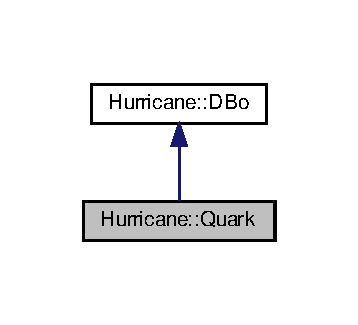
\includegraphics[width=172pt]{classHurricane_1_1Quark__inherit__graph}
\end{center}
\end{figure}
\doxysubsection*{Public Member Functions}
\begin{DoxyCompactItemize}
\item 
const \mbox{\hyperlink{classHurricane_1_1Occurrence}{Occurrence}} \& \mbox{\hyperlink{classHurricane_1_1Quark_a22ee192574dae1546ec17d6c549b2ca0}{get\+Occurrence}} () const
\end{DoxyCompactItemize}


\doxysubsection{Detailed Description}
\mbox{\hyperlink{classHurricane_1_1Quark}{Quark}} description ({\bfseries{API}}) 

\hypertarget{classHurricane_1_1Quark_secQuarkIntro}{}\doxysubsection{Introduction}\label{classHurricane_1_1Quark_secQuarkIntro}
As explained in the Occurence class, occurences are very simple objects used to designate any entity of the virtually unfolded hierarchy. However, those occurences, which are built and deleted very easily, are very volatile objects to which we can\textquotesingle{}t, of course, attach properties directly.

But the usefullness of occurences lies in their ability to attach them properties.

In order to do that, properties must be stored in a secure place, where they can be found when needed. That is the purpose of quarks \+: they are data base objects and then can own the properties of the occurences.\hypertarget{classHurricane_1_1Quark_secQuarkImportant}{}\doxysubsection{Important}\label{classHurricane_1_1Quark_secQuarkImportant}
A quark designates all occurences refering to the same entity of the virtually unfolded hierarchy.

This means that a property put on an occurence can be recovered by an other occurence refering the same entity of the virtually unfolded hierarchy.\hypertarget{classHurricane_1_1Quark_secQuarkConstructionAndDestruction}{}\doxysubsection{Construction and destruction}\label{classHurricane_1_1Quark_secQuarkConstructionAndDestruction}
Quarks being completely managed by the system, there is no constructor provided.

They are themselves volatile because they need to exist only if there is at least a property attached to them (you must never store pointers to them !).

An occurence may have, during its life, different quarks representing it.

Nevertheless, it is possible to destroy a quark. This one will carry away with it the destruction of all its owned properties (like any other data base object). This is equivalent to destroying the properties associated to the occurences whom it is the unique representative. Conceptually, it is wiser to use the call \+: {\bfseries{occurence.\+clear\+Properties()}} which does the same.\hypertarget{classHurricane_1_1Quark_secQuarkExample}{}\doxysubsection{Example}\label{classHurricane_1_1Quark_secQuarkExample}
The following sample code shows how to print the set of owners of a shared property \+: 
\begin{DoxyCode}{0}
\DoxyCodeLine{Property* \textcolor{keyword}{property} = ...; \textcolor{comment}{// we get a property}}
\DoxyCodeLine{ }
\DoxyCodeLine{\textcolor{keywordflow}{if} (is\_a<SharedPropery*>(property)) \{}
\DoxyCodeLine{  forEach(DBo*, idbo, ((SharedProperty*)property)getOwners()) \{}
\DoxyCodeLine{    \textcolor{keywordflow}{if} (not is\_a<Quark*>(*idbo))}
\DoxyCodeLine{      cerr << *idbo << endl;}
\DoxyCodeLine{    \textcolor{keywordflow}{else}}
\DoxyCodeLine{      cerr << ((Quark*)*idbo)-\/>getOccurence() << endl;}
\DoxyCodeLine{  \}}
\DoxyCodeLine{\}}

\end{DoxyCode}
 

\doxysubsection{Member Function Documentation}
\mbox{\Hypertarget{classHurricane_1_1Quark_a22ee192574dae1546ec17d6c549b2ca0}\label{classHurricane_1_1Quark_a22ee192574dae1546ec17d6c549b2ca0}} 
\index{Hurricane::Quark@{Hurricane::Quark}!getOccurrence@{getOccurrence}}
\index{getOccurrence@{getOccurrence}!Hurricane::Quark@{Hurricane::Quark}}
\doxysubsubsection{\texorpdfstring{getOccurrence()}{getOccurrence()}}
{\footnotesize\ttfamily const \mbox{\hyperlink{classHurricane_1_1Occurrence}{Occurrence}} \& Hurricane\+::\+Quark\+::get\+Occurrence (\begin{DoxyParamCaption}{ }\end{DoxyParamCaption}) const\hspace{0.3cm}{\ttfamily [inline]}}

{\bfseries{Returns\+:}} an occurence of which this quark is a representative. 

The documentation for this class was generated from the following files\+:\begin{DoxyCompactItemize}
\item 
Quark.\+h\item 
Quark.\+dox\end{DoxyCompactItemize}

\hypertarget{classHurricane_1_1Query}{}\section{Hurricane\+:\+:Query Class Reference}
\label{classHurricane_1_1Query}\index{Hurricane\+::\+Query@{Hurricane\+::\+Query}}


\mbox{\hyperlink{classHurricane_1_1Query}{Query}} description ({\bfseries A\+PI})  


\subsection*{Public Types}
\begin{DoxyCompactItemize}
\item 
enum \mbox{\hyperlink{classHurricane_1_1Query_a003517b82eaba58104d1749cf344eaa9}{Query\+Filter}} \{ \newline
\mbox{\hyperlink{classHurricane_1_1Query_a003517b82eaba58104d1749cf344eaa9a427b951cfef3fbeb3c2baa9abc4eae83}{Do\+Master\+Cells}} = 1, 
\newline
\mbox{\hyperlink{classHurricane_1_1Query_a003517b82eaba58104d1749cf344eaa9a2a1f9d4cf126b86694e05152a1b04ee9}{Do\+Terminal\+Cells}} = 2, 
\newline
\mbox{\hyperlink{classHurricane_1_1Query_a003517b82eaba58104d1749cf344eaa9a7b591d72b86f94f90d212746ed8f9f56}{Do\+Components}} = 4, 
\newline
\mbox{\hyperlink{classHurricane_1_1Query_a003517b82eaba58104d1749cf344eaa9ade01b12e4a2af3bfba0440caa557619a}{Do\+Markers}} = 8, 
\newline
\mbox{\hyperlink{classHurricane_1_1Query_a003517b82eaba58104d1749cf344eaa9a3671f7b32f05ccbd1db6e6e94da040e4}{Do\+Rubbers}} = 16, 
\newline
\mbox{\hyperlink{classHurricane_1_1Query_a003517b82eaba58104d1749cf344eaa9a241d98f4f53e908f113669540ef4288c}{Do\+Extension\+Gos}} = 32, 
\newline
\mbox{\hyperlink{classHurricane_1_1Query_a003517b82eaba58104d1749cf344eaa9ad3d1832e33bbdd8fa1e07ce622c984ec}{Do\+All}}
 \}
\end{DoxyCompactItemize}
\subsection*{Public Member Functions}
\begin{DoxyCompactItemize}
\item 
\mbox{\hyperlink{classHurricane_1_1Query_a999eaaaf34672fb056df14629d3197d1}{Query}} ()
\item 
virtual \mbox{\hyperlink{classHurricane_1_1Query_acd18d98c6bf30dd049916508a397391a}{$\sim$\+Query}} ()
\item 
unsigned int \mbox{\hyperlink{classHurricane_1_1Query_a7aac7fbdc96df19e7249bf8993eb355f}{get\+Start\+Level}} () const
\item 
unsigned int \mbox{\hyperlink{classHurricane_1_1Query_a3544d22dbb0685208c590cef09412796}{get\+Stop\+Level}} () const
\item 
size\+\_\+t \mbox{\hyperlink{classHurricane_1_1Query_afb81080617e5b4d3c2bedf1bf8b2ebd8}{get\+Depth}} () const
\item 
const \mbox{\hyperlink{classHurricane_1_1Transformation}{Transformation}} \& \mbox{\hyperlink{classHurricane_1_1Query_aabe2c0588f95c30a3acfec8fed269be4}{get\+Transformation}} () const
\item 
const \mbox{\hyperlink{classHurricane_1_1Box}{Box}} \& \mbox{\hyperlink{classHurricane_1_1Query_a666c44432d3f5717f2fee5f57a281bdd}{get\+Area}} () const
\item 
const \mbox{\hyperlink{classHurricane_1_1BasicLayer}{Basic\+Layer}} $\ast$ \mbox{\hyperlink{classHurricane_1_1Query_ac683152bccef813184e572806e4c14f4}{get\+Basic\+Layer}} () const
\item 
\mbox{\hyperlink{classHurricane_1_1Cell}{Cell}} $\ast$ \mbox{\hyperlink{classHurricane_1_1Query_add13f7ff193df6ce5223f9761b6cba69}{get\+Master\+Cell}} ()
\item 
\mbox{\hyperlink{classHurricane_1_1Instance}{Instance}} $\ast$ \mbox{\hyperlink{classHurricane_1_1Query_a459b9f175f77fce91963eeb192c6e018}{get\+Instance}} ()
\item 
\mbox{\hyperlink{classHurricane_1_1Path}{Path}} \mbox{\hyperlink{classHurricane_1_1Query_ae6be93b35a9174b2e7b656853f450021}{get\+Path}} () const
\item 
virtual bool \mbox{\hyperlink{classHurricane_1_1Query_aeff0c9c1ef8b787a3f1460ea55db2947}{has\+Go\+Callback}} () const
\item 
virtual bool \mbox{\hyperlink{classHurricane_1_1Query_a4f121b05f722a661b88bb8a0dc981024}{has\+Marker\+Callback}} () const
\item 
virtual bool \mbox{\hyperlink{classHurricane_1_1Query_a5d49250d46dea1542bc3034f3eb1daee}{has\+Rubber\+Callback}} () const
\item 
virtual bool \mbox{\hyperlink{classHurricane_1_1Query_abd8ff8d187e4499e625feb12c68e9b29}{has\+Extension\+Go\+Callback}} () const
\item 
virtual bool \mbox{\hyperlink{classHurricane_1_1Query_a7ebb7b16bab183cd4508dc5639bd12ab}{has\+Master\+Cell\+Callback}} () const
\item 
virtual void \mbox{\hyperlink{classHurricane_1_1Query_a59007148bd0afa0405801f341e7e4139}{go\+Callback}} (\mbox{\hyperlink{classHurricane_1_1Go}{Go}} $\ast$)=0
\item 
virtual void \mbox{\hyperlink{classHurricane_1_1Query_a4ad5bf076073f107189d4b7ee48f040e}{marker\+Callback}} (Marker $\ast$)
\item 
virtual void \mbox{\hyperlink{classHurricane_1_1Query_acec322581e35c1556ce706aa5ea66aa3}{rubber\+Callback}} (\mbox{\hyperlink{classHurricane_1_1Rubber}{Rubber}} $\ast$)
\item 
virtual void \mbox{\hyperlink{classHurricane_1_1Query_a75b87e969b64caaf24ec058c0d2dfa68}{extension\+Go\+Callback}} (\mbox{\hyperlink{classHurricane_1_1Go}{Go}} $\ast$)=0
\item 
virtual void \mbox{\hyperlink{classHurricane_1_1Query_abaf97e93c7fa96469adf64f7865938b4}{master\+Cell\+Callback}} ()=0
\item 
void \mbox{\hyperlink{classHurricane_1_1Query_a70fce1e5b7754f1ec11097ad5b9ecfc9}{set\+Query}} (\mbox{\hyperlink{classHurricane_1_1Cell}{Cell}} $\ast$cell, const \mbox{\hyperlink{classHurricane_1_1Box}{Box}} \&area, const \mbox{\hyperlink{classHurricane_1_1Transformation}{Transformation}} \&transformation, const \mbox{\hyperlink{classHurricane_1_1BasicLayer}{Basic\+Layer}} $\ast$basic\+Layer, Extension\+Slice\+::\+Mask extension\+Mask, Mask filter, \mbox{\hyperlink{group__DbUGroup_ga4fbfa3e8c89347af76c9628ea06c4146}{Db\+U\+::\+Unit}} threshold=0)
\item 
void \mbox{\hyperlink{classHurricane_1_1Query_a36378e1604e484450a3ccee0ececcff7}{set\+Cell}} (\mbox{\hyperlink{classHurricane_1_1Cell}{Cell}} $\ast$cell)
\item 
void \mbox{\hyperlink{classHurricane_1_1Query_ac41de6b1535c256c4929c075769890b1}{set\+Area}} (const \mbox{\hyperlink{classHurricane_1_1Box}{Box}} \&area)
\item 
void \mbox{\hyperlink{classHurricane_1_1Query_a885360fc2f351fc3612c7dda363b5131}{set\+Transformation}} (const \mbox{\hyperlink{classHurricane_1_1Transformation}{Transformation}} \&transformation)
\item 
virtual void \mbox{\hyperlink{classHurricane_1_1Query_ac3718c4e2cd4d5e80af32558285481af}{set\+Basic\+Layer}} (const \mbox{\hyperlink{classHurricane_1_1BasicLayer}{Basic\+Layer}} $\ast$basic\+Layer)
\item 
void \mbox{\hyperlink{classHurricane_1_1Query_af7f83fd3aefe1b5654f9bdd3566fe0d4}{set\+Extension\+Mask}} (Extension\+Slice\+::\+Mask mode)
\item 
void \mbox{\hyperlink{classHurricane_1_1Query_a457a0cda5ea5ad849a46aefce2514963}{set\+Filter}} (Mask mode)
\item 
void \mbox{\hyperlink{classHurricane_1_1Query_a8c4bc1bcfae942042ccb90a46b6fb510}{set\+Start\+Level}} (unsigned int level)
\item 
void \mbox{\hyperlink{classHurricane_1_1Query_a70359c71d7dc7e3f17d0a29c8208c92f}{set\+Stop\+Level}} (unsigned int level)
\item 
virtual void \mbox{\hyperlink{classHurricane_1_1Query_a2ca5bf71c7b35e14c4a64488a5e21bc6}{do\+Query}} ()
\end{DoxyCompactItemize}


\subsection{Detailed Description}
\mbox{\hyperlink{classHurricane_1_1Query}{Query}} description ({\bfseries A\+PI}) 

\hypertarget{classHurricane_1_1Query_secQueryIntro}{}\subsection{Introduction}\label{classHurricane_1_1Query_secQueryIntro}
The \mbox{\hyperlink{classHurricane_1_1Query}{Query}} is a part of the trans-\/hierarchical mechanism. A \mbox{\hyperlink{classHurricane_1_1Query}{Query}} performs a walktrough over all the Occurrences of objects under a determined area, thus providing a virtual flattening service. Please note that only placed objects (i.\+e. inserted in a \mbox{\hyperlink{classHurricane_1_1QuadTree}{Quad\+Tree}}) are took into account.

To use the \mbox{\hyperlink{classHurricane_1_1Query}{Query}} class the user has to create derived classes and overload the various callbacks. At least the following pure virtual methods must be overloaded\+:
\begin{DoxyItemize}
\item \mbox{\hyperlink{classHurricane_1_1Query_abaf97e93c7fa96469adf64f7865938b4}{Query\+::master\+Cell\+Callback()}}.
\item \mbox{\hyperlink{classHurricane_1_1Query_a59007148bd0afa0405801f341e7e4139}{Query\+::go\+Callback()}}.
\item \mbox{\hyperlink{classHurricane_1_1Query_a75b87e969b64caaf24ec058c0d2dfa68}{Query\+::extension\+Go\+Callback()}}.
\end{DoxyItemize}\hypertarget{classHurricane_1_1Query_secQueryParameters}{}\subsection{sec\+Query\+Parameters}\label{classHurricane_1_1Query_secQueryParameters}
A query walkthrough is defined by the following parameters\+:
\begin{DoxyItemize}
\item The starting hierarchical level\+: only objects with a hierarchical depth greater or equal will be explored. The top level \mbox{\hyperlink{classHurricane_1_1Cell}{Cell}} has a depth of {\itshape zero}, the master \mbox{\hyperlink{classHurricane_1_1Cell}{Cell}} of the instances a depth of {\itshape one} and so on.
\item The stoping hierarchical level\+: only objects with a hierarchical depth lesser or equal will be considered.
\item The top \mbox{\hyperlink{classHurricane_1_1Cell}{Cell}} on which to start.
\item The area to consider on the top \mbox{\hyperlink{classHurricane_1_1Cell}{Cell}}.
\item A transformation to apply on the top \mbox{\hyperlink{classHurricane_1_1Cell}{Cell}}.
\item A \mbox{\hyperlink{classHurricane_1_1BasicLayer}{Basic\+Layer}} to select only the Gos containing it.
\item An Extension\+Slice\+::\+Mask to select which user-\/defined slice to process.
\item A Mask, to select which kind of \mbox{\hyperlink{classHurricane_1_1Go}{Go}} to process. 
\end{DoxyItemize}

\subsection{Member Enumeration Documentation}
\mbox{\Hypertarget{classHurricane_1_1Query_a003517b82eaba58104d1749cf344eaa9}\label{classHurricane_1_1Query_a003517b82eaba58104d1749cf344eaa9}} 
\index{Hurricane\+::\+Query@{Hurricane\+::\+Query}!Query\+Filter@{Query\+Filter}}
\index{Query\+Filter@{Query\+Filter}!Hurricane\+::\+Query@{Hurricane\+::\+Query}}
\subsubsection{\texorpdfstring{Query\+Filter}{QueryFilter}}
{\footnotesize\ttfamily enum \mbox{\hyperlink{classHurricane_1_1Query_a003517b82eaba58104d1749cf344eaa9}{Hurricane\+::\+Query\+::\+Query\+Filter}}}

Set of flags to specify on which types of objects the \mbox{\hyperlink{classHurricane_1_1Query}{Query}} must iterate. \begin{DoxyEnumFields}{Enumerator}
\raisebox{\heightof{T}}[0pt][0pt]{\index{Do\+Master\+Cells@{Do\+Master\+Cells}!Hurricane\+::\+Query@{Hurricane\+::\+Query}}\index{Hurricane\+::\+Query@{Hurricane\+::\+Query}!Do\+Master\+Cells@{Do\+Master\+Cells}}}\mbox{\Hypertarget{classHurricane_1_1Query_a003517b82eaba58104d1749cf344eaa9a427b951cfef3fbeb3c2baa9abc4eae83}\label{classHurricane_1_1Query_a003517b82eaba58104d1749cf344eaa9a427b951cfef3fbeb3c2baa9abc4eae83}} 
Do\+Master\+Cells&Activate the call of the \mbox{\hyperlink{classHurricane_1_1Query_abaf97e93c7fa96469adf64f7865938b4}{Query\+::master\+Cell\+Callback()}}. \\
\hline

\raisebox{\heightof{T}}[0pt][0pt]{\index{Do\+Terminal\+Cells@{Do\+Terminal\+Cells}!Hurricane\+::\+Query@{Hurricane\+::\+Query}}\index{Hurricane\+::\+Query@{Hurricane\+::\+Query}!Do\+Terminal\+Cells@{Do\+Terminal\+Cells}}}\mbox{\Hypertarget{classHurricane_1_1Query_a003517b82eaba58104d1749cf344eaa9a2a1f9d4cf126b86694e05152a1b04ee9}\label{classHurricane_1_1Query_a003517b82eaba58104d1749cf344eaa9a2a1f9d4cf126b86694e05152a1b04ee9}} 
Do\+Terminal\+Cells&Activate the call of the \mbox{\hyperlink{classHurricane_1_1Query_abaf97e93c7fa96469adf64f7865938b4}{Query\+::master\+Cell\+Callback()}}, but only on leaf \mbox{\hyperlink{classHurricane_1_1Cell}{Cell}} of the hierarchy. \\
\hline

\raisebox{\heightof{T}}[0pt][0pt]{\index{Do\+Components@{Do\+Components}!Hurricane\+::\+Query@{Hurricane\+::\+Query}}\index{Hurricane\+::\+Query@{Hurricane\+::\+Query}!Do\+Components@{Do\+Components}}}\mbox{\Hypertarget{classHurricane_1_1Query_a003517b82eaba58104d1749cf344eaa9a7b591d72b86f94f90d212746ed8f9f56}\label{classHurricane_1_1Query_a003517b82eaba58104d1749cf344eaa9a7b591d72b86f94f90d212746ed8f9f56}} 
Do\+Components&Activate the call of the \mbox{\hyperlink{classHurricane_1_1Query_a59007148bd0afa0405801f341e7e4139}{Query\+::go\+Callback()}}. \\
\hline

\raisebox{\heightof{T}}[0pt][0pt]{\index{Do\+Markers@{Do\+Markers}!Hurricane\+::\+Query@{Hurricane\+::\+Query}}\index{Hurricane\+::\+Query@{Hurricane\+::\+Query}!Do\+Markers@{Do\+Markers}}}\mbox{\Hypertarget{classHurricane_1_1Query_a003517b82eaba58104d1749cf344eaa9ade01b12e4a2af3bfba0440caa557619a}\label{classHurricane_1_1Query_a003517b82eaba58104d1749cf344eaa9ade01b12e4a2af3bfba0440caa557619a}} 
Do\+Markers&Activate the call of the \mbox{\hyperlink{classHurricane_1_1Query_a4ad5bf076073f107189d4b7ee48f040e}{Query\+::marker\+Callback()}}. \\
\hline

\raisebox{\heightof{T}}[0pt][0pt]{\index{Do\+Rubbers@{Do\+Rubbers}!Hurricane\+::\+Query@{Hurricane\+::\+Query}}\index{Hurricane\+::\+Query@{Hurricane\+::\+Query}!Do\+Rubbers@{Do\+Rubbers}}}\mbox{\Hypertarget{classHurricane_1_1Query_a003517b82eaba58104d1749cf344eaa9a3671f7b32f05ccbd1db6e6e94da040e4}\label{classHurricane_1_1Query_a003517b82eaba58104d1749cf344eaa9a3671f7b32f05ccbd1db6e6e94da040e4}} 
Do\+Rubbers&Activate the call of the \mbox{\hyperlink{classHurricane_1_1Query_acec322581e35c1556ce706aa5ea66aa3}{Query\+::rubber\+Callback()}}. \\
\hline

\raisebox{\heightof{T}}[0pt][0pt]{\index{Do\+Extension\+Gos@{Do\+Extension\+Gos}!Hurricane\+::\+Query@{Hurricane\+::\+Query}}\index{Hurricane\+::\+Query@{Hurricane\+::\+Query}!Do\+Extension\+Gos@{Do\+Extension\+Gos}}}\mbox{\Hypertarget{classHurricane_1_1Query_a003517b82eaba58104d1749cf344eaa9a241d98f4f53e908f113669540ef4288c}\label{classHurricane_1_1Query_a003517b82eaba58104d1749cf344eaa9a241d98f4f53e908f113669540ef4288c}} 
Do\+Extension\+Gos&Activate the call of the \mbox{\hyperlink{classHurricane_1_1Query_a75b87e969b64caaf24ec058c0d2dfa68}{Query\+::extension\+Go\+Callback()}}. \\
\hline

\raisebox{\heightof{T}}[0pt][0pt]{\index{Do\+All@{Do\+All}!Hurricane\+::\+Query@{Hurricane\+::\+Query}}\index{Hurricane\+::\+Query@{Hurricane\+::\+Query}!Do\+All@{Do\+All}}}\mbox{\Hypertarget{classHurricane_1_1Query_a003517b82eaba58104d1749cf344eaa9ad3d1832e33bbdd8fa1e07ce622c984ec}\label{classHurricane_1_1Query_a003517b82eaba58104d1749cf344eaa9ad3d1832e33bbdd8fa1e07ce622c984ec}} 
Do\+All&Activate all the callbacks at once. \\
\hline

\end{DoxyEnumFields}


\subsection{Constructor \& Destructor Documentation}
\mbox{\Hypertarget{classHurricane_1_1Query_a999eaaaf34672fb056df14629d3197d1}\label{classHurricane_1_1Query_a999eaaaf34672fb056df14629d3197d1}} 
\index{Hurricane\+::\+Query@{Hurricane\+::\+Query}!Query@{Query}}
\index{Query@{Query}!Hurricane\+::\+Query@{Hurricane\+::\+Query}}
\subsubsection{\texorpdfstring{Query()}{Query()}}
{\footnotesize\ttfamily Hurricane\+::\+Query\+::\+Query (\begin{DoxyParamCaption}{ }\end{DoxyParamCaption})}

Default constructor. Initialisation is done through \mbox{\hyperlink{classHurricane_1_1Query_a70fce1e5b7754f1ec11097ad5b9ecfc9}{Query\+::set\+Query()}}. \mbox{\Hypertarget{classHurricane_1_1Query_acd18d98c6bf30dd049916508a397391a}\label{classHurricane_1_1Query_acd18d98c6bf30dd049916508a397391a}} 
\index{Hurricane\+::\+Query@{Hurricane\+::\+Query}!````~Query@{$\sim$\+Query}}
\index{````~Query@{$\sim$\+Query}!Hurricane\+::\+Query@{Hurricane\+::\+Query}}
\subsubsection{\texorpdfstring{$\sim$\+Query()}{~Query()}}
{\footnotesize\ttfamily Hurricane\+::\+Query\+::$\sim$\+Query (\begin{DoxyParamCaption}{ }\end{DoxyParamCaption})\hspace{0.3cm}{\ttfamily [virtual]}}

Default destructor. 

\subsection{Member Function Documentation}
\mbox{\Hypertarget{classHurricane_1_1Query_a7aac7fbdc96df19e7249bf8993eb355f}\label{classHurricane_1_1Query_a7aac7fbdc96df19e7249bf8993eb355f}} 
\index{Hurricane\+::\+Query@{Hurricane\+::\+Query}!get\+Start\+Level@{get\+Start\+Level}}
\index{get\+Start\+Level@{get\+Start\+Level}!Hurricane\+::\+Query@{Hurricane\+::\+Query}}
\subsubsection{\texorpdfstring{get\+Start\+Level()}{getStartLevel()}}
{\footnotesize\ttfamily unsigned int Hurricane\+::\+Query\+::get\+Start\+Level (\begin{DoxyParamCaption}{ }\end{DoxyParamCaption}) const\hspace{0.3cm}{\ttfamily [inline]}}

The hierarchical level from which we start to consider objects. \mbox{\Hypertarget{classHurricane_1_1Query_a3544d22dbb0685208c590cef09412796}\label{classHurricane_1_1Query_a3544d22dbb0685208c590cef09412796}} 
\index{Hurricane\+::\+Query@{Hurricane\+::\+Query}!get\+Stop\+Level@{get\+Stop\+Level}}
\index{get\+Stop\+Level@{get\+Stop\+Level}!Hurricane\+::\+Query@{Hurricane\+::\+Query}}
\subsubsection{\texorpdfstring{get\+Stop\+Level()}{getStopLevel()}}
{\footnotesize\ttfamily unsigned int Hurricane\+::\+Query\+::get\+Stop\+Level (\begin{DoxyParamCaption}{ }\end{DoxyParamCaption}) const\hspace{0.3cm}{\ttfamily [inline]}}

The hierarchical level from which we stop to consider objects. \mbox{\Hypertarget{classHurricane_1_1Query_afb81080617e5b4d3c2bedf1bf8b2ebd8}\label{classHurricane_1_1Query_afb81080617e5b4d3c2bedf1bf8b2ebd8}} 
\index{Hurricane\+::\+Query@{Hurricane\+::\+Query}!get\+Depth@{get\+Depth}}
\index{get\+Depth@{get\+Depth}!Hurricane\+::\+Query@{Hurricane\+::\+Query}}
\subsubsection{\texorpdfstring{get\+Depth()}{getDepth()}}
{\footnotesize\ttfamily size\+\_\+t Hurricane\+::\+Query\+::get\+Depth (\begin{DoxyParamCaption}{ }\end{DoxyParamCaption}) const\hspace{0.3cm}{\ttfamily [inline]}}

The hierarchical depth of the current \mbox{\hyperlink{classHurricane_1_1Query}{Query}} walkthrough. \mbox{\Hypertarget{classHurricane_1_1Query_aabe2c0588f95c30a3acfec8fed269be4}\label{classHurricane_1_1Query_aabe2c0588f95c30a3acfec8fed269be4}} 
\index{Hurricane\+::\+Query@{Hurricane\+::\+Query}!get\+Transformation@{get\+Transformation}}
\index{get\+Transformation@{get\+Transformation}!Hurricane\+::\+Query@{Hurricane\+::\+Query}}
\subsubsection{\texorpdfstring{get\+Transformation()}{getTransformation()}}
{\footnotesize\ttfamily const \mbox{\hyperlink{classHurricane_1_1Transformation}{Transformation}} \& Hurricane\+::\+Query\+::get\+Transformation (\begin{DoxyParamCaption}{ }\end{DoxyParamCaption}) const\hspace{0.3cm}{\ttfamily [inline]}}

The cumulative transformation of the master cell currently under exploration. \mbox{\Hypertarget{classHurricane_1_1Query_a666c44432d3f5717f2fee5f57a281bdd}\label{classHurricane_1_1Query_a666c44432d3f5717f2fee5f57a281bdd}} 
\index{Hurricane\+::\+Query@{Hurricane\+::\+Query}!get\+Area@{get\+Area}}
\index{get\+Area@{get\+Area}!Hurricane\+::\+Query@{Hurricane\+::\+Query}}
\subsubsection{\texorpdfstring{get\+Area()}{getArea()}}
{\footnotesize\ttfamily const \mbox{\hyperlink{classHurricane_1_1Box}{Box}} \& Hurricane\+::\+Query\+::get\+Area (\begin{DoxyParamCaption}{ }\end{DoxyParamCaption}) const\hspace{0.3cm}{\ttfamily [inline]}}

The area to explore, expressed in the coordinates system of the current master cell under exploration. This is the starting area with the inverse of the current transformation applied. \mbox{\Hypertarget{classHurricane_1_1Query_ac683152bccef813184e572806e4c14f4}\label{classHurricane_1_1Query_ac683152bccef813184e572806e4c14f4}} 
\index{Hurricane\+::\+Query@{Hurricane\+::\+Query}!get\+Basic\+Layer@{get\+Basic\+Layer}}
\index{get\+Basic\+Layer@{get\+Basic\+Layer}!Hurricane\+::\+Query@{Hurricane\+::\+Query}}
\subsubsection{\texorpdfstring{get\+Basic\+Layer()}{getBasicLayer()}}
{\footnotesize\ttfamily const \mbox{\hyperlink{classHurricane_1_1BasicLayer}{Basic\+Layer}} $\ast$ Hurricane\+::\+Query\+::get\+Basic\+Layer (\begin{DoxyParamCaption}{ }\end{DoxyParamCaption}) const\hspace{0.3cm}{\ttfamily [inline]}}

The \mbox{\hyperlink{classHurricane_1_1BasicLayer}{Basic\+Layer}} we are filtering with. \mbox{\Hypertarget{classHurricane_1_1Query_add13f7ff193df6ce5223f9761b6cba69}\label{classHurricane_1_1Query_add13f7ff193df6ce5223f9761b6cba69}} 
\index{Hurricane\+::\+Query@{Hurricane\+::\+Query}!get\+Master\+Cell@{get\+Master\+Cell}}
\index{get\+Master\+Cell@{get\+Master\+Cell}!Hurricane\+::\+Query@{Hurricane\+::\+Query}}
\subsubsection{\texorpdfstring{get\+Master\+Cell()}{getMasterCell()}}
{\footnotesize\ttfamily \mbox{\hyperlink{classHurricane_1_1Cell}{Cell}} $\ast$ Hurricane\+::\+Query\+::get\+Master\+Cell (\begin{DoxyParamCaption}{ }\end{DoxyParamCaption})\hspace{0.3cm}{\ttfamily [inline]}}

The master \mbox{\hyperlink{classHurricane_1_1Cell}{Cell}} currently under exploration. \mbox{\Hypertarget{classHurricane_1_1Query_a459b9f175f77fce91963eeb192c6e018}\label{classHurricane_1_1Query_a459b9f175f77fce91963eeb192c6e018}} 
\index{Hurricane\+::\+Query@{Hurricane\+::\+Query}!get\+Instance@{get\+Instance}}
\index{get\+Instance@{get\+Instance}!Hurricane\+::\+Query@{Hurricane\+::\+Query}}
\subsubsection{\texorpdfstring{get\+Instance()}{getInstance()}}
{\footnotesize\ttfamily \mbox{\hyperlink{classHurricane_1_1Instance}{Instance}} $\ast$ Hurricane\+::\+Query\+::get\+Instance (\begin{DoxyParamCaption}{ }\end{DoxyParamCaption})\hspace{0.3cm}{\ttfamily [inline]}}

The \mbox{\hyperlink{classHurricane_1_1Instance}{Instance}} currently under exploration. \mbox{\Hypertarget{classHurricane_1_1Query_ae6be93b35a9174b2e7b656853f450021}\label{classHurricane_1_1Query_ae6be93b35a9174b2e7b656853f450021}} 
\index{Hurricane\+::\+Query@{Hurricane\+::\+Query}!get\+Path@{get\+Path}}
\index{get\+Path@{get\+Path}!Hurricane\+::\+Query@{Hurricane\+::\+Query}}
\subsubsection{\texorpdfstring{get\+Path()}{getPath()}}
{\footnotesize\ttfamily \mbox{\hyperlink{classHurricane_1_1Path}{Path}} Hurricane\+::\+Query\+::get\+Path (\begin{DoxyParamCaption}{ }\end{DoxyParamCaption}) const\hspace{0.3cm}{\ttfamily [inline]}}

The instanciation path between the instance currently under inspection and the top cell. \mbox{\Hypertarget{classHurricane_1_1Query_aeff0c9c1ef8b787a3f1460ea55db2947}\label{classHurricane_1_1Query_aeff0c9c1ef8b787a3f1460ea55db2947}} 
\index{Hurricane\+::\+Query@{Hurricane\+::\+Query}!has\+Go\+Callback@{has\+Go\+Callback}}
\index{has\+Go\+Callback@{has\+Go\+Callback}!Hurricane\+::\+Query@{Hurricane\+::\+Query}}
\subsubsection{\texorpdfstring{has\+Go\+Callback()}{hasGoCallback()}}
{\footnotesize\ttfamily bool Hurricane\+::\+Query\+::has\+Go\+Callback (\begin{DoxyParamCaption}{ }\end{DoxyParamCaption}) const\hspace{0.3cm}{\ttfamily [virtual]}}

Tells wether the \mbox{\hyperlink{classHurricane_1_1Go}{Go}} callback is present and should be called. \mbox{\Hypertarget{classHurricane_1_1Query_a4f121b05f722a661b88bb8a0dc981024}\label{classHurricane_1_1Query_a4f121b05f722a661b88bb8a0dc981024}} 
\index{Hurricane\+::\+Query@{Hurricane\+::\+Query}!has\+Marker\+Callback@{has\+Marker\+Callback}}
\index{has\+Marker\+Callback@{has\+Marker\+Callback}!Hurricane\+::\+Query@{Hurricane\+::\+Query}}
\subsubsection{\texorpdfstring{has\+Marker\+Callback()}{hasMarkerCallback()}}
{\footnotesize\ttfamily bool Hurricane\+::\+Query\+::has\+Marker\+Callback (\begin{DoxyParamCaption}{ }\end{DoxyParamCaption}) const\hspace{0.3cm}{\ttfamily [virtual]}}

Tells wether the Marker callback is present and should be called. \mbox{\Hypertarget{classHurricane_1_1Query_a5d49250d46dea1542bc3034f3eb1daee}\label{classHurricane_1_1Query_a5d49250d46dea1542bc3034f3eb1daee}} 
\index{Hurricane\+::\+Query@{Hurricane\+::\+Query}!has\+Rubber\+Callback@{has\+Rubber\+Callback}}
\index{has\+Rubber\+Callback@{has\+Rubber\+Callback}!Hurricane\+::\+Query@{Hurricane\+::\+Query}}
\subsubsection{\texorpdfstring{has\+Rubber\+Callback()}{hasRubberCallback()}}
{\footnotesize\ttfamily bool Hurricane\+::\+Query\+::has\+Rubber\+Callback (\begin{DoxyParamCaption}{ }\end{DoxyParamCaption}) const\hspace{0.3cm}{\ttfamily [virtual]}}

Tells wether the \mbox{\hyperlink{classHurricane_1_1Rubber}{Rubber}} callback is present and should be called. \mbox{\Hypertarget{classHurricane_1_1Query_abd8ff8d187e4499e625feb12c68e9b29}\label{classHurricane_1_1Query_abd8ff8d187e4499e625feb12c68e9b29}} 
\index{Hurricane\+::\+Query@{Hurricane\+::\+Query}!has\+Extension\+Go\+Callback@{has\+Extension\+Go\+Callback}}
\index{has\+Extension\+Go\+Callback@{has\+Extension\+Go\+Callback}!Hurricane\+::\+Query@{Hurricane\+::\+Query}}
\subsubsection{\texorpdfstring{has\+Extension\+Go\+Callback()}{hasExtensionGoCallback()}}
{\footnotesize\ttfamily bool Hurricane\+::\+Query\+::has\+Extension\+Go\+Callback (\begin{DoxyParamCaption}{ }\end{DoxyParamCaption}) const\hspace{0.3cm}{\ttfamily [virtual]}}

Tells wether the Extension\+Go callback is present and should be called. \mbox{\Hypertarget{classHurricane_1_1Query_a7ebb7b16bab183cd4508dc5639bd12ab}\label{classHurricane_1_1Query_a7ebb7b16bab183cd4508dc5639bd12ab}} 
\index{Hurricane\+::\+Query@{Hurricane\+::\+Query}!has\+Master\+Cell\+Callback@{has\+Master\+Cell\+Callback}}
\index{has\+Master\+Cell\+Callback@{has\+Master\+Cell\+Callback}!Hurricane\+::\+Query@{Hurricane\+::\+Query}}
\subsubsection{\texorpdfstring{has\+Master\+Cell\+Callback()}{hasMasterCellCallback()}}
{\footnotesize\ttfamily bool Hurricane\+::\+Query\+::has\+Master\+Cell\+Callback (\begin{DoxyParamCaption}{ }\end{DoxyParamCaption}) const\hspace{0.3cm}{\ttfamily [virtual]}}

Tells wether the master \mbox{\hyperlink{classHurricane_1_1Cell}{Cell}} callback is present and should be called. \mbox{\Hypertarget{classHurricane_1_1Query_a59007148bd0afa0405801f341e7e4139}\label{classHurricane_1_1Query_a59007148bd0afa0405801f341e7e4139}} 
\index{Hurricane\+::\+Query@{Hurricane\+::\+Query}!go\+Callback@{go\+Callback}}
\index{go\+Callback@{go\+Callback}!Hurricane\+::\+Query@{Hurricane\+::\+Query}}
\subsubsection{\texorpdfstring{go\+Callback()}{goCallback()}}
{\footnotesize\ttfamily void Hurricane\+::\+Query\+::go\+Callback (\begin{DoxyParamCaption}\item[{\mbox{\hyperlink{classHurricane_1_1Go}{Go}} $\ast$}]{ }\end{DoxyParamCaption})\hspace{0.3cm}{\ttfamily [pure virtual]}}

The method called on each encountered \mbox{\hyperlink{classHurricane_1_1Go}{Go}}. This is a pure virtual method which must be overloaded in derived classes. \mbox{\Hypertarget{classHurricane_1_1Query_a4ad5bf076073f107189d4b7ee48f040e}\label{classHurricane_1_1Query_a4ad5bf076073f107189d4b7ee48f040e}} 
\index{Hurricane\+::\+Query@{Hurricane\+::\+Query}!marker\+Callback@{marker\+Callback}}
\index{marker\+Callback@{marker\+Callback}!Hurricane\+::\+Query@{Hurricane\+::\+Query}}
\subsubsection{\texorpdfstring{marker\+Callback()}{markerCallback()}}
{\footnotesize\ttfamily void Hurricane\+::\+Query\+::marker\+Callback (\begin{DoxyParamCaption}\item[{Marker $\ast$}]{ }\end{DoxyParamCaption})\hspace{0.3cm}{\ttfamily [virtual]}}

The method called on each encountered Marker. A default implementation is provided, which does absolutely nothing. \mbox{\Hypertarget{classHurricane_1_1Query_acec322581e35c1556ce706aa5ea66aa3}\label{classHurricane_1_1Query_acec322581e35c1556ce706aa5ea66aa3}} 
\index{Hurricane\+::\+Query@{Hurricane\+::\+Query}!rubber\+Callback@{rubber\+Callback}}
\index{rubber\+Callback@{rubber\+Callback}!Hurricane\+::\+Query@{Hurricane\+::\+Query}}
\subsubsection{\texorpdfstring{rubber\+Callback()}{rubberCallback()}}
{\footnotesize\ttfamily void Hurricane\+::\+Query\+::rubber\+Callback (\begin{DoxyParamCaption}\item[{\mbox{\hyperlink{classHurricane_1_1Rubber}{Rubber}} $\ast$}]{ }\end{DoxyParamCaption})\hspace{0.3cm}{\ttfamily [virtual]}}

The method called on each encountered \mbox{\hyperlink{classHurricane_1_1Rubber}{Rubber}}. A default implementation is provided, which does absolutely nothing. \mbox{\Hypertarget{classHurricane_1_1Query_a75b87e969b64caaf24ec058c0d2dfa68}\label{classHurricane_1_1Query_a75b87e969b64caaf24ec058c0d2dfa68}} 
\index{Hurricane\+::\+Query@{Hurricane\+::\+Query}!extension\+Go\+Callback@{extension\+Go\+Callback}}
\index{extension\+Go\+Callback@{extension\+Go\+Callback}!Hurricane\+::\+Query@{Hurricane\+::\+Query}}
\subsubsection{\texorpdfstring{extension\+Go\+Callback()}{extensionGoCallback()}}
{\footnotesize\ttfamily void Hurricane\+::\+Query\+::extension\+Go\+Callback (\begin{DoxyParamCaption}\item[{\mbox{\hyperlink{classHurricane_1_1Go}{Go}} $\ast$}]{ }\end{DoxyParamCaption})\hspace{0.3cm}{\ttfamily [pure virtual]}}

The method called on each encountered Extension\+Go. This is a pure virtual method which must be overloaded in derived classes. \mbox{\Hypertarget{classHurricane_1_1Query_abaf97e93c7fa96469adf64f7865938b4}\label{classHurricane_1_1Query_abaf97e93c7fa96469adf64f7865938b4}} 
\index{Hurricane\+::\+Query@{Hurricane\+::\+Query}!master\+Cell\+Callback@{master\+Cell\+Callback}}
\index{master\+Cell\+Callback@{master\+Cell\+Callback}!Hurricane\+::\+Query@{Hurricane\+::\+Query}}
\subsubsection{\texorpdfstring{master\+Cell\+Callback()}{masterCellCallback()}}
{\footnotesize\ttfamily void Hurricane\+::\+Query\+::master\+Cell\+Callback (\begin{DoxyParamCaption}{ }\end{DoxyParamCaption})\hspace{0.3cm}{\ttfamily [pure virtual]}}

The method called on each encountered master \mbox{\hyperlink{classHurricane_1_1Cell}{Cell}}. The \mbox{\hyperlink{classHurricane_1_1Cell}{Cell}} is not passed as parameter as it is directly accessible through Query\+::get\+Cell(). This is a pure virtual method which must be overloaded in derived classes. \mbox{\Hypertarget{classHurricane_1_1Query_a70fce1e5b7754f1ec11097ad5b9ecfc9}\label{classHurricane_1_1Query_a70fce1e5b7754f1ec11097ad5b9ecfc9}} 
\index{Hurricane\+::\+Query@{Hurricane\+::\+Query}!set\+Query@{set\+Query}}
\index{set\+Query@{set\+Query}!Hurricane\+::\+Query@{Hurricane\+::\+Query}}
\subsubsection{\texorpdfstring{set\+Query()}{setQuery()}}
{\footnotesize\ttfamily void Hurricane\+::\+Query\+::set\+Query (\begin{DoxyParamCaption}\item[{\mbox{\hyperlink{classHurricane_1_1Cell}{Cell}} $\ast$}]{cell,  }\item[{const \mbox{\hyperlink{classHurricane_1_1Box}{Box}} \&}]{area,  }\item[{const \mbox{\hyperlink{classHurricane_1_1Transformation}{Transformation}} \&}]{transformation,  }\item[{const \mbox{\hyperlink{classHurricane_1_1BasicLayer}{Basic\+Layer}} $\ast$}]{basic\+Layer,  }\item[{Extension\+Slice\+::\+Mask}]{extension\+Mask,  }\item[{Mask}]{filter,  }\item[{\mbox{\hyperlink{group__DbUGroup_ga4fbfa3e8c89347af76c9628ea06c4146}{Db\+U\+::\+Unit}}}]{threshold = {\ttfamily 0} }\end{DoxyParamCaption})}


\begin{DoxyParams}{Parameters}
{\em cell} & The top \mbox{\hyperlink{classHurricane_1_1Cell}{Cell}} on which to start the \mbox{\hyperlink{classHurricane_1_1Query}{Query}}. \\
\hline
{\em area} & The area under which objects are queried. \\
\hline
{\em transformation} & An initial transformation to apply to {\ttfamily cell}. \\
\hline
{\em basic\+Layer} & Consider only objects containing this \mbox{\hyperlink{classHurricane_1_1BasicLayer}{Basic\+Layer}}. \\
\hline
{\em extension\+Mask} & Consider only Extension\+Go matching this mask. \\
\hline
{\em filter} & Consider only objects of certain types, as defined in Query\+Filter.\\
\hline
\end{DoxyParams}
Initialize the basic parameters of the \mbox{\hyperlink{classHurricane_1_1Query}{Query}}. Those parameters can be changed individually afterwards with specific mutators. \mbox{\Hypertarget{classHurricane_1_1Query_a36378e1604e484450a3ccee0ececcff7}\label{classHurricane_1_1Query_a36378e1604e484450a3ccee0ececcff7}} 
\index{Hurricane\+::\+Query@{Hurricane\+::\+Query}!set\+Cell@{set\+Cell}}
\index{set\+Cell@{set\+Cell}!Hurricane\+::\+Query@{Hurricane\+::\+Query}}
\subsubsection{\texorpdfstring{set\+Cell()}{setCell()}}
{\footnotesize\ttfamily void Hurricane\+::\+Query\+::set\+Cell (\begin{DoxyParamCaption}\item[{\mbox{\hyperlink{classHurricane_1_1Cell}{Cell}} $\ast$}]{cell }\end{DoxyParamCaption})\hspace{0.3cm}{\ttfamily [inline]}}

Change the top \mbox{\hyperlink{classHurricane_1_1Cell}{Cell}} on which to perform the \mbox{\hyperlink{classHurricane_1_1Query}{Query}}. \mbox{\Hypertarget{classHurricane_1_1Query_ac41de6b1535c256c4929c075769890b1}\label{classHurricane_1_1Query_ac41de6b1535c256c4929c075769890b1}} 
\index{Hurricane\+::\+Query@{Hurricane\+::\+Query}!set\+Area@{set\+Area}}
\index{set\+Area@{set\+Area}!Hurricane\+::\+Query@{Hurricane\+::\+Query}}
\subsubsection{\texorpdfstring{set\+Area()}{setArea()}}
{\footnotesize\ttfamily void Hurricane\+::\+Query\+::set\+Area (\begin{DoxyParamCaption}\item[{const \mbox{\hyperlink{classHurricane_1_1Box}{Box}} \&}]{box }\end{DoxyParamCaption})\hspace{0.3cm}{\ttfamily [inline]}}

Change the top area to query. \mbox{\Hypertarget{classHurricane_1_1Query_a885360fc2f351fc3612c7dda363b5131}\label{classHurricane_1_1Query_a885360fc2f351fc3612c7dda363b5131}} 
\index{Hurricane\+::\+Query@{Hurricane\+::\+Query}!set\+Transformation@{set\+Transformation}}
\index{set\+Transformation@{set\+Transformation}!Hurricane\+::\+Query@{Hurricane\+::\+Query}}
\subsubsection{\texorpdfstring{set\+Transformation()}{setTransformation()}}
{\footnotesize\ttfamily void Hurricane\+::\+Query\+::set\+Transformation (\begin{DoxyParamCaption}\item[{const \mbox{\hyperlink{classHurricane_1_1Transformation}{Transformation}} \&}]{transformation }\end{DoxyParamCaption})\hspace{0.3cm}{\ttfamily [inline]}}

Change the transformation applied to the top level \mbox{\hyperlink{classHurricane_1_1Cell}{Cell}}. \mbox{\Hypertarget{classHurricane_1_1Query_ac3718c4e2cd4d5e80af32558285481af}\label{classHurricane_1_1Query_ac3718c4e2cd4d5e80af32558285481af}} 
\index{Hurricane\+::\+Query@{Hurricane\+::\+Query}!set\+Basic\+Layer@{set\+Basic\+Layer}}
\index{set\+Basic\+Layer@{set\+Basic\+Layer}!Hurricane\+::\+Query@{Hurricane\+::\+Query}}
\subsubsection{\texorpdfstring{set\+Basic\+Layer()}{setBasicLayer()}}
{\footnotesize\ttfamily void Hurricane\+::\+Query\+::set\+Basic\+Layer (\begin{DoxyParamCaption}\item[{const \mbox{\hyperlink{classHurricane_1_1BasicLayer}{Basic\+Layer}} $\ast$}]{basic\+Layer }\end{DoxyParamCaption})\hspace{0.3cm}{\ttfamily [virtual]}}

Change the \mbox{\hyperlink{classHurricane_1_1BasicLayer}{Basic\+Layer}} selector. \mbox{\Hypertarget{classHurricane_1_1Query_af7f83fd3aefe1b5654f9bdd3566fe0d4}\label{classHurricane_1_1Query_af7f83fd3aefe1b5654f9bdd3566fe0d4}} 
\index{Hurricane\+::\+Query@{Hurricane\+::\+Query}!set\+Extension\+Mask@{set\+Extension\+Mask}}
\index{set\+Extension\+Mask@{set\+Extension\+Mask}!Hurricane\+::\+Query@{Hurricane\+::\+Query}}
\subsubsection{\texorpdfstring{set\+Extension\+Mask()}{setExtensionMask()}}
{\footnotesize\ttfamily void Hurricane\+::\+Query\+::set\+Extension\+Mask (\begin{DoxyParamCaption}\item[{Extension\+Slice\+::\+Mask}]{mode }\end{DoxyParamCaption})\hspace{0.3cm}{\ttfamily [inline]}}

Change the filtering mask for Extension\+Slice. \mbox{\Hypertarget{classHurricane_1_1Query_a457a0cda5ea5ad849a46aefce2514963}\label{classHurricane_1_1Query_a457a0cda5ea5ad849a46aefce2514963}} 
\index{Hurricane\+::\+Query@{Hurricane\+::\+Query}!set\+Filter@{set\+Filter}}
\index{set\+Filter@{set\+Filter}!Hurricane\+::\+Query@{Hurricane\+::\+Query}}
\subsubsection{\texorpdfstring{set\+Filter()}{setFilter()}}
{\footnotesize\ttfamily void Hurricane\+::\+Query\+::set\+Filter (\begin{DoxyParamCaption}\item[{Mask}]{mode }\end{DoxyParamCaption})\hspace{0.3cm}{\ttfamily [inline]}}

Change the filtering mask for object types. \mbox{\Hypertarget{classHurricane_1_1Query_a8c4bc1bcfae942042ccb90a46b6fb510}\label{classHurricane_1_1Query_a8c4bc1bcfae942042ccb90a46b6fb510}} 
\index{Hurricane\+::\+Query@{Hurricane\+::\+Query}!set\+Start\+Level@{set\+Start\+Level}}
\index{set\+Start\+Level@{set\+Start\+Level}!Hurricane\+::\+Query@{Hurricane\+::\+Query}}
\subsubsection{\texorpdfstring{set\+Start\+Level()}{setStartLevel()}}
{\footnotesize\ttfamily void Hurricane\+::\+Query\+::set\+Start\+Level (\begin{DoxyParamCaption}\item[{unsigned int}]{level }\end{DoxyParamCaption})\hspace{0.3cm}{\ttfamily [inline]}}

Change the starting depth level. \mbox{\Hypertarget{classHurricane_1_1Query_a70359c71d7dc7e3f17d0a29c8208c92f}\label{classHurricane_1_1Query_a70359c71d7dc7e3f17d0a29c8208c92f}} 
\index{Hurricane\+::\+Query@{Hurricane\+::\+Query}!set\+Stop\+Level@{set\+Stop\+Level}}
\index{set\+Stop\+Level@{set\+Stop\+Level}!Hurricane\+::\+Query@{Hurricane\+::\+Query}}
\subsubsection{\texorpdfstring{set\+Stop\+Level()}{setStopLevel()}}
{\footnotesize\ttfamily void Hurricane\+::\+Query\+::set\+Stop\+Level (\begin{DoxyParamCaption}\item[{unsigned int}]{level }\end{DoxyParamCaption})\hspace{0.3cm}{\ttfamily [inline]}}

Change the stoping depth level. \mbox{\Hypertarget{classHurricane_1_1Query_a2ca5bf71c7b35e14c4a64488a5e21bc6}\label{classHurricane_1_1Query_a2ca5bf71c7b35e14c4a64488a5e21bc6}} 
\index{Hurricane\+::\+Query@{Hurricane\+::\+Query}!do\+Query@{do\+Query}}
\index{do\+Query@{do\+Query}!Hurricane\+::\+Query@{Hurricane\+::\+Query}}
\subsubsection{\texorpdfstring{do\+Query()}{doQuery()}}
{\footnotesize\ttfamily void Hurricane\+::\+Query\+::do\+Query (\begin{DoxyParamCaption}{ }\end{DoxyParamCaption})\hspace{0.3cm}{\ttfamily [virtual]}}

Perform the actual \mbox{\hyperlink{classHurricane_1_1Query}{Query}}. 

The documentation for this class was generated from the following files\+:\begin{DoxyCompactItemize}
\item 
Query.\+h\item 
Query.\+dox\end{DoxyCompactItemize}

\hypertarget{classHurricane_1_1RegularLayer}{}\doxysection{Hurricane\+::Regular\+Layer Class Reference}
\label{classHurricane_1_1RegularLayer}\index{Hurricane::RegularLayer@{Hurricane::RegularLayer}}


\mbox{\hyperlink{classHurricane_1_1RegularLayer}{Regular\+Layer}} description ({\bfseries{API}})  




Inheritance diagram for Hurricane\+::Regular\+Layer\+:\nopagebreak
\begin{figure}[H]
\begin{center}
\leavevmode
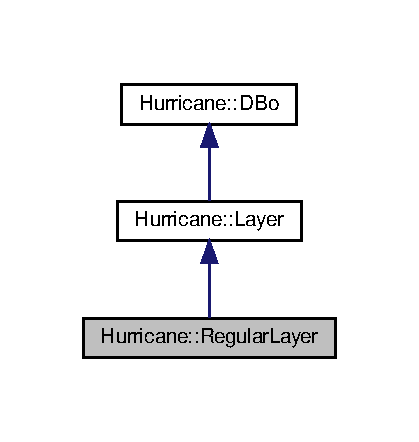
\includegraphics[width=201pt]{classHurricane_1_1RegularLayer__inherit__graph}
\end{center}
\end{figure}
\doxysubsection*{Public Member Functions}
\begin{DoxyCompactItemize}
\item 
\mbox{\hyperlink{classHurricane_1_1BasicLayer}{Basic\+Layer}} $\ast$ \mbox{\hyperlink{classHurricane_1_1RegularLayer_a148c5839b544c2a0aa5d25be5958dfaf}{get\+Basic\+Layer}} () const
\end{DoxyCompactItemize}
\doxysubsection*{Static Public Member Functions}
\begin{DoxyCompactItemize}
\item 
static \mbox{\hyperlink{classHurricane_1_1RegularLayer}{Regular\+Layer}} $\ast$ \mbox{\hyperlink{classHurricane_1_1RegularLayer_a6b40a35fec1c4fc168d608b8b96c8477}{create}} (\mbox{\hyperlink{classHurricane_1_1Technology}{Technology}} $\ast$technology, const \mbox{\hyperlink{classHurricane_1_1Name}{Name}} \&name, \mbox{\hyperlink{classHurricane_1_1BasicLayer}{Basic\+Layer}} $\ast$layer)
\end{DoxyCompactItemize}
\doxysubsection*{Additional Inherited Members}


\doxysubsection{Detailed Description}
\mbox{\hyperlink{classHurricane_1_1RegularLayer}{Regular\+Layer}} description ({\bfseries{API}}) 

For a more complete description of the Layers objects, please refer to \mbox{\hyperlink{classHurricane_1_1Layer_secLayerIntro}{Layer Introduction}}.

\mbox{\hyperlink{classHurricane_1_1RegularLayer}{Regular\+Layer}} is a symbolic layer that contains exactly one \mbox{\hyperlink{classHurricane_1_1BasicLayer}{Basic\+Layer}}. The accessors functions\+: 
\begin{DoxyItemize}
\item Regular\+Layer\+::get\+Top() 
\item Regular\+Layer\+::get\+Bottom() 
\item Regular\+Layer\+::get\+Opposite() 
\end{DoxyItemize}All returns that \mbox{\hyperlink{classHurricane_1_1BasicLayer}{Basic\+Layer}}.

It have one enclose, extention cap \& extension width. 

\doxysubsection{Member Function Documentation}
\mbox{\Hypertarget{classHurricane_1_1RegularLayer_a6b40a35fec1c4fc168d608b8b96c8477}\label{classHurricane_1_1RegularLayer_a6b40a35fec1c4fc168d608b8b96c8477}} 
\index{Hurricane::RegularLayer@{Hurricane::RegularLayer}!create@{create}}
\index{create@{create}!Hurricane::RegularLayer@{Hurricane::RegularLayer}}
\doxysubsubsection{\texorpdfstring{create()}{create()}}
{\footnotesize\ttfamily \mbox{\hyperlink{classHurricane_1_1RegularLayer}{Regular\+Layer}} $\ast$ Hurricane\+::\+Regular\+Layer\+::create (\begin{DoxyParamCaption}\item[{\mbox{\hyperlink{classHurricane_1_1Technology}{Technology}} $\ast$}]{technology,  }\item[{const \mbox{\hyperlink{classHurricane_1_1Name}{Name}} \&}]{name,  }\item[{\mbox{\hyperlink{classHurricane_1_1BasicLayer}{Basic\+Layer}} $\ast$}]{layer }\end{DoxyParamCaption})\hspace{0.3cm}{\ttfamily [static]}}

creates and returns a new regular layer named {\ttfamily $<$name$>$}.

\begin{DoxyParagraph}{Caution\+: Throws an exception if the technology is null, if the name is }
empty, if a layer of same name already exists or if we overflow the capacity of the bit field associated to the layer mask. 
\end{DoxyParagraph}
\mbox{\Hypertarget{classHurricane_1_1RegularLayer_a148c5839b544c2a0aa5d25be5958dfaf}\label{classHurricane_1_1RegularLayer_a148c5839b544c2a0aa5d25be5958dfaf}} 
\index{Hurricane::RegularLayer@{Hurricane::RegularLayer}!getBasicLayer@{getBasicLayer}}
\index{getBasicLayer@{getBasicLayer}!Hurricane::RegularLayer@{Hurricane::RegularLayer}}
\doxysubsubsection{\texorpdfstring{getBasicLayer()}{getBasicLayer()}}
{\footnotesize\ttfamily \mbox{\hyperlink{classHurricane_1_1BasicLayer}{Basic\+Layer}} $\ast$ Hurricane\+::\+Regular\+Layer\+::get\+Basic\+Layer (\begin{DoxyParamCaption}{ }\end{DoxyParamCaption}) const\hspace{0.3cm}{\ttfamily [inline]}}

{\bfseries{Returns\+:}} the one associated \mbox{\hyperlink{classHurricane_1_1BasicLayer}{Basic\+Layer}}. 

The documentation for this class was generated from the following files\+:\begin{DoxyCompactItemize}
\item 
Regular\+Layer.\+h\item 
Regular\+Layer.\+dox\end{DoxyCompactItemize}

\hypertarget{classHurricane_1_1Relation}{}\doxysection{Hurricane\+::Relation Class Reference}
\label{classHurricane_1_1Relation}\index{Hurricane::Relation@{Hurricane::Relation}}


\mbox{\hyperlink{classHurricane_1_1Relation}{Relation}} description ({\bfseries{API}})  




Inheritance diagram for Hurricane\+::Relation\+:\nopagebreak
\begin{figure}[H]
\begin{center}
\leavevmode
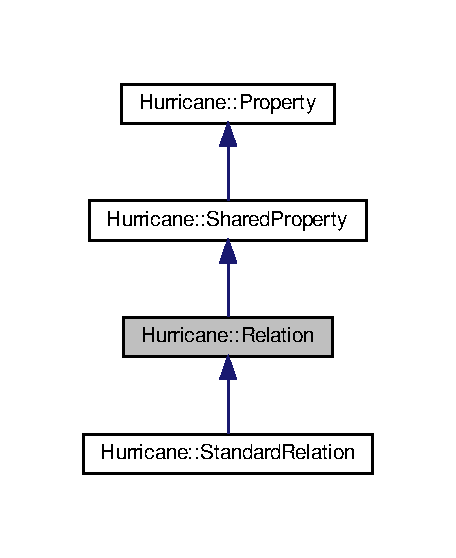
\includegraphics[width=219pt]{classHurricane_1_1Relation__inherit__graph}
\end{center}
\end{figure}
\doxysubsection*{Additional Inherited Members}


\doxysubsection{Detailed Description}
\mbox{\hyperlink{classHurricane_1_1Relation}{Relation}} description ({\bfseries{API}}) 

The documentation for this class was generated from the following file\+:\begin{DoxyCompactItemize}
\item 
Relation.\+h\end{DoxyCompactItemize}

\hypertarget{classHurricane_1_1RoutingPad}{}\doxysection{Hurricane\+::Routing\+Pad Class Reference}
\label{classHurricane_1_1RoutingPad}\index{Hurricane::RoutingPad@{Hurricane::RoutingPad}}


\mbox{\hyperlink{classHurricane_1_1RoutingPad}{Routing\+Pad}} description ({\bfseries{API}})  




Inheritance diagram for Hurricane\+::Routing\+Pad\+:\nopagebreak
\begin{figure}[H]
\begin{center}
\leavevmode
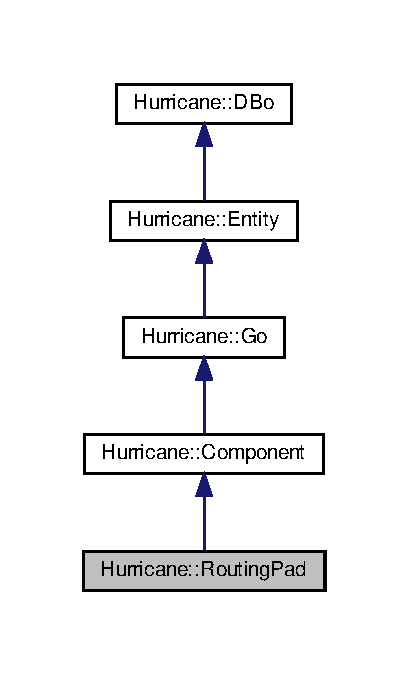
\includegraphics[width=196pt]{classHurricane_1_1RoutingPad__inherit__graph}
\end{center}
\end{figure}
\doxysubsection*{Public Types}
\begin{DoxyCompactItemize}
\item 
enum \mbox{\hyperlink{classHurricane_1_1RoutingPad_a69f37f0b06b9bfd758d9be42c71e2bd4}{Flags}} \{ \newline
\mbox{\hyperlink{classHurricane_1_1RoutingPad_a69f37f0b06b9bfd758d9be42c71e2bd4add72642d150e901835fa7d66d40e327d}{Biggest\+Area}} = (1 $<$$<$ 0)
, \newline
\mbox{\hyperlink{classHurricane_1_1RoutingPad_a69f37f0b06b9bfd758d9be42c71e2bd4a8f7993760a105713a97abdfb05eee852}{Highest\+Layer}} = (1 $<$$<$ 1)
, \newline
\mbox{\hyperlink{classHurricane_1_1RoutingPad_a69f37f0b06b9bfd758d9be42c71e2bd4a14c89f0c4ca6f4108b7f2ac30ab885a6}{Lowest\+Layer}} = (1 $<$$<$ 2)
, \newline
\mbox{\hyperlink{classHurricane_1_1RoutingPad_a69f37f0b06b9bfd758d9be42c71e2bd4aa2db526191b29a7e094bff309e27ef4c}{Component\+Selection}} = Biggest\+Area$\vert$\+Highest\+Layer$\vert$\+Lowest\+Layer
, \newline
\mbox{\hyperlink{classHurricane_1_1RoutingPad_a69f37f0b06b9bfd758d9be42c71e2bd4a8fd74358022a29aab828700c8f7347ba}{Show\+Warning}} = (1 $<$$<$ 4)
 \}
\item 
typedef \mbox{\hyperlink{classHurricane_1_1Component}{Component}} \mbox{\hyperlink{classHurricane_1_1RoutingPad_a53bed3713fe846a351621d2022bc6b68}{Inherit}}
\end{DoxyCompactItemize}
\doxysubsection*{Public Member Functions}
\begin{DoxyCompactItemize}
\item 
bool \mbox{\hyperlink{classHurricane_1_1RoutingPad_a3e94730dded06e5953087755f0551b73}{is\+Placed\+Occurrence}} (unsigned int flags) const
\item 
\mbox{\hyperlink{classHurricane_1_1Occurrence}{Occurrence}} \mbox{\hyperlink{classHurricane_1_1RoutingPad_a2767550364ef01c772f3270850ec052f}{get\+Occurrence}} () const
\item 
\mbox{\hyperlink{classHurricane_1_1Occurrence}{Occurrence}} \mbox{\hyperlink{classHurricane_1_1RoutingPad_a30190c50577ce47727dec11f5423a85b}{get\+Plug\+Occurrence}} ()
\item 
virtual const \mbox{\hyperlink{classHurricane_1_1Layer}{Layer}} $\ast$ \mbox{\hyperlink{classHurricane_1_1RoutingPad_a7f1e300e4148556fa223e623738d79d4}{get\+Layer}} () const
\item 
virtual \mbox{\hyperlink{classHurricane_1_1DbU_a4fbfa3e8c89347af76c9628ea06c4146}{Db\+U\+::\+Unit}} \mbox{\hyperlink{classHurricane_1_1RoutingPad_a5c9c00c648bd0d24e1a8b0876ab442df}{getX}} () const
\item 
virtual \mbox{\hyperlink{classHurricane_1_1DbU_a4fbfa3e8c89347af76c9628ea06c4146}{Db\+U\+::\+Unit}} \mbox{\hyperlink{classHurricane_1_1RoutingPad_aede4c04a7f893b1e5478b164b6eaae2d}{getY}} () const
\item 
virtual \mbox{\hyperlink{classHurricane_1_1Box}{Box}} \mbox{\hyperlink{classHurricane_1_1RoutingPad_a2cc2894b5e1c82b725dedcf1978dc773}{get\+Bounding\+Box}} () const
\item 
virtual \mbox{\hyperlink{classHurricane_1_1Point}{Point}} \mbox{\hyperlink{classHurricane_1_1RoutingPad_ad254b92749146a0eaaa7ed8f33fac4da}{get\+Center}} () const
\item 
\mbox{\hyperlink{classHurricane_1_1Point}{Point}} \mbox{\hyperlink{classHurricane_1_1RoutingPad_acc706fecb615230387a73ed8a7384c8e}{get\+Source\+Position}} () const
\item 
\mbox{\hyperlink{classHurricane_1_1Point}{Point}} \mbox{\hyperlink{classHurricane_1_1RoutingPad_a8de215adabb4a3330d02339c38dd6d4b}{get\+Target\+Position}} () const
\item 
\mbox{\hyperlink{classHurricane_1_1DbU_a4fbfa3e8c89347af76c9628ea06c4146}{Db\+U\+::\+Unit}} \mbox{\hyperlink{classHurricane_1_1RoutingPad_ae80e8f84f5806582905f6695f5cc43df}{get\+SourceX}} () const
\item 
\mbox{\hyperlink{classHurricane_1_1DbU_a4fbfa3e8c89347af76c9628ea06c4146}{Db\+U\+::\+Unit}} \mbox{\hyperlink{classHurricane_1_1RoutingPad_a75983ff3507f4cbf2aaa4e3132eac987}{get\+SourceY}} () const
\item 
\mbox{\hyperlink{classHurricane_1_1DbU_a4fbfa3e8c89347af76c9628ea06c4146}{Db\+U\+::\+Unit}} \mbox{\hyperlink{classHurricane_1_1RoutingPad_a3c0f5056b20515d308c2945ab692bce5}{get\+TargetX}} () const
\item 
\mbox{\hyperlink{classHurricane_1_1DbU_a4fbfa3e8c89347af76c9628ea06c4146}{Db\+U\+::\+Unit}} \mbox{\hyperlink{classHurricane_1_1RoutingPad_a41a9c831d668377fc0c5e628f66465a0}{get\+TargetY}} () const
\item 
virtual void \mbox{\hyperlink{classHurricane_1_1RoutingPad_a41bf66ffda0c0ceaaebc67acd72d5b36}{translate}} (const \mbox{\hyperlink{classHurricane_1_1DbU_a4fbfa3e8c89347af76c9628ea06c4146}{Db\+U\+::\+Unit}} \&dx, const \mbox{\hyperlink{classHurricane_1_1DbU_a4fbfa3e8c89347af76c9628ea06c4146}{Db\+U\+::\+Unit}} \&dy)
\item 
void \mbox{\hyperlink{classHurricane_1_1RoutingPad_a9f448ad4f05f6995edc4a5ab50501586}{set\+External\+Component}} (\mbox{\hyperlink{classHurricane_1_1Component}{Component}} $\ast$)
\item 
\mbox{\hyperlink{classHurricane_1_1Component}{Component}} $\ast$ \mbox{\hyperlink{classHurricane_1_1RoutingPad_a410992ef75c40f9a898c36f39a7d1a1a}{set\+On\+Best\+Component}} (unsigned int flags)
\item 
void \mbox{\hyperlink{classHurricane_1_1RoutingPad_a1fcb0951f5f9505c6978bf498f78fce9}{restore\+Plug\+Occurrence}} ()
\end{DoxyCompactItemize}
\doxysubsection*{Static Public Member Functions}
\begin{DoxyCompactItemize}
\item 
static \mbox{\hyperlink{classHurricane_1_1RoutingPad}{Routing\+Pad}} $\ast$ \mbox{\hyperlink{classHurricane_1_1RoutingPad_a87c3a286477f81b9c791dc24104a3e51}{create}} (\mbox{\hyperlink{classHurricane_1_1Net}{Net}} $\ast$, \mbox{\hyperlink{classHurricane_1_1Occurrence}{Occurrence}}, unsigned int flags=0)
\item 
static \mbox{\hyperlink{classHurricane_1_1RoutingPad}{Routing\+Pad}} $\ast$ \mbox{\hyperlink{classHurricane_1_1RoutingPad_a1883e5711b5700cd7d1024f1cff6abb0}{create}} (\mbox{\hyperlink{classHurricane_1_1Pin}{Pin}} $\ast$)
\end{DoxyCompactItemize}


\doxysubsection{Detailed Description}
\mbox{\hyperlink{classHurricane_1_1RoutingPad}{Routing\+Pad}} description ({\bfseries{API}}) 

\hypertarget{classHurricane_1_1RoutingPad_secRoutingPadIntro}{}\doxysubsection{Introduction}\label{classHurricane_1_1RoutingPad_secRoutingPadIntro}
The \mbox{\hyperlink{classHurricane_1_1RoutingPad}{Routing\+Pad}} is a part of the trans-\/hierarchical mechanism. It allows to connect a \mbox{\hyperlink{classHurricane_1_1Net}{Net}} from the top-\/level netlist to a plug in an \mbox{\hyperlink{classHurricane_1_1Instance}{Instance}} at any level inside the hierarchy, through a \mbox{\hyperlink{classHurricane_1_1Plug}{Plug}} \mbox{\hyperlink{classHurricane_1_1Occurrence}{Occurrence}}. \mbox{\hyperlink{classHurricane_1_1RoutingPad}{Routing\+Pad}} can also be created from \mbox{\hyperlink{classHurricane_1_1Pin}{Pin}} or \mbox{\hyperlink{classHurricane_1_1Contact}{Contact}} Occurrences.

When the \mbox{\hyperlink{classHurricane_1_1RoutingPad}{Routing\+Pad}} is created using a \mbox{\hyperlink{classHurricane_1_1Plug}{Plug}} \mbox{\hyperlink{classHurricane_1_1Occurrence}{Occurrence}}, it can be set afterward to any of master net external \mbox{\hyperlink{classHurricane_1_1Component}{Component}}. A utility method \mbox{\hyperlink{classHurricane_1_1RoutingPad_a410992ef75c40f9a898c36f39a7d1a1a}{Routing\+Pad\+::set\+On\+Best\+Component()}} is also provided to automatically set the \mbox{\hyperlink{classHurricane_1_1RoutingPad}{Routing\+Pad}} on a \mbox{\hyperlink{classHurricane_1_1Component}{Component}} matching criteria of surface or layer level.

The position of the \mbox{\hyperlink{classHurricane_1_1RoutingPad}{Routing\+Pad}} is fixed relatively from the instances in it\textquotesingle{}s occurrence path and the entity it refers. The reference point used on the entity is it\textquotesingle{}s center whether it is a segment, a pin or a plug. In the later case, it is the center of the cell. 

\doxysubsection{Member Typedef Documentation}
\mbox{\Hypertarget{classHurricane_1_1RoutingPad_a53bed3713fe846a351621d2022bc6b68}\label{classHurricane_1_1RoutingPad_a53bed3713fe846a351621d2022bc6b68}} 
\index{Hurricane::RoutingPad@{Hurricane::RoutingPad}!Inherit@{Inherit}}
\index{Inherit@{Inherit}!Hurricane::RoutingPad@{Hurricane::RoutingPad}}
\doxysubsubsection{\texorpdfstring{Inherit}{Inherit}}
{\footnotesize\ttfamily \mbox{\hyperlink{classHurricane_1_1RoutingPad_a53bed3713fe846a351621d2022bc6b68}{Hurricane\+::\+Routing\+Pad\+::\+Inherit}}}

Useful for calling upon methods of the base class without knowing it. 

\doxysubsection{Member Enumeration Documentation}
\mbox{\Hypertarget{classHurricane_1_1RoutingPad_a69f37f0b06b9bfd758d9be42c71e2bd4}\label{classHurricane_1_1RoutingPad_a69f37f0b06b9bfd758d9be42c71e2bd4}} 
\index{Hurricane::RoutingPad@{Hurricane::RoutingPad}!Flags@{Flags}}
\index{Flags@{Flags}!Hurricane::RoutingPad@{Hurricane::RoutingPad}}
\doxysubsubsection{\texorpdfstring{Flags}{Flags}}
{\footnotesize\ttfamily enum \mbox{\hyperlink{classHurricane_1_1RoutingPad_a69f37f0b06b9bfd758d9be42c71e2bd4}{Hurricane\+::\+Routing\+Pad\+::\+Flags}}}

Set of flags to choose how to select the external component of a \mbox{\hyperlink{classHurricane_1_1RoutingPad}{Routing\+Pad}} to be anchored on. \begin{DoxyEnumFields}{Enumerator}
\raisebox{\heightof{T}}[0pt][0pt]{\index{BiggestArea@{BiggestArea}!Hurricane::RoutingPad@{Hurricane::RoutingPad}}\index{Hurricane::RoutingPad@{Hurricane::RoutingPad}!BiggestArea@{BiggestArea}}}\mbox{\Hypertarget{classHurricane_1_1RoutingPad_a69f37f0b06b9bfd758d9be42c71e2bd4add72642d150e901835fa7d66d40e327d}\label{classHurricane_1_1RoutingPad_a69f37f0b06b9bfd758d9be42c71e2bd4add72642d150e901835fa7d66d40e327d}} 
Biggest\+Area&Select the external \mbox{\hyperlink{classHurricane_1_1Component}{Component}} of biggest area. \\
\hline

\raisebox{\heightof{T}}[0pt][0pt]{\index{HighestLayer@{HighestLayer}!Hurricane::RoutingPad@{Hurricane::RoutingPad}}\index{Hurricane::RoutingPad@{Hurricane::RoutingPad}!HighestLayer@{HighestLayer}}}\mbox{\Hypertarget{classHurricane_1_1RoutingPad_a69f37f0b06b9bfd758d9be42c71e2bd4a8f7993760a105713a97abdfb05eee852}\label{classHurricane_1_1RoutingPad_a69f37f0b06b9bfd758d9be42c71e2bd4a8f7993760a105713a97abdfb05eee852}} 
Highest\+Layer&Select the external \mbox{\hyperlink{classHurricane_1_1Component}{Component}} of in the highest layer. \\
\hline

\raisebox{\heightof{T}}[0pt][0pt]{\index{LowestLayer@{LowestLayer}!Hurricane::RoutingPad@{Hurricane::RoutingPad}}\index{Hurricane::RoutingPad@{Hurricane::RoutingPad}!LowestLayer@{LowestLayer}}}\mbox{\Hypertarget{classHurricane_1_1RoutingPad_a69f37f0b06b9bfd758d9be42c71e2bd4a14c89f0c4ca6f4108b7f2ac30ab885a6}\label{classHurricane_1_1RoutingPad_a69f37f0b06b9bfd758d9be42c71e2bd4a14c89f0c4ca6f4108b7f2ac30ab885a6}} 
Lowest\+Layer&Select the external \mbox{\hyperlink{classHurricane_1_1Component}{Component}} of in the lowest layer. \\
\hline

\raisebox{\heightof{T}}[0pt][0pt]{\index{ComponentSelection@{ComponentSelection}!Hurricane::RoutingPad@{Hurricane::RoutingPad}}\index{Hurricane::RoutingPad@{Hurricane::RoutingPad}!ComponentSelection@{ComponentSelection}}}\mbox{\Hypertarget{classHurricane_1_1RoutingPad_a69f37f0b06b9bfd758d9be42c71e2bd4aa2db526191b29a7e094bff309e27ef4c}\label{classHurricane_1_1RoutingPad_a69f37f0b06b9bfd758d9be42c71e2bd4aa2db526191b29a7e094bff309e27ef4c}} 
Component\+Selection&A mask to filter bit parts of a flag belonging to component selection. \\
\hline

\raisebox{\heightof{T}}[0pt][0pt]{\index{ShowWarning@{ShowWarning}!Hurricane::RoutingPad@{Hurricane::RoutingPad}}\index{Hurricane::RoutingPad@{Hurricane::RoutingPad}!ShowWarning@{ShowWarning}}}\mbox{\Hypertarget{classHurricane_1_1RoutingPad_a69f37f0b06b9bfd758d9be42c71e2bd4a8fd74358022a29aab828700c8f7347ba}\label{classHurricane_1_1RoutingPad_a69f37f0b06b9bfd758d9be42c71e2bd4a8fd74358022a29aab828700c8f7347ba}} 
Show\+Warning&Whether to display a warning or not while checking the instances placement. \\
\hline

\end{DoxyEnumFields}


\doxysubsection{Member Function Documentation}
\mbox{\Hypertarget{classHurricane_1_1RoutingPad_a87c3a286477f81b9c791dc24104a3e51}\label{classHurricane_1_1RoutingPad_a87c3a286477f81b9c791dc24104a3e51}} 
\index{Hurricane::RoutingPad@{Hurricane::RoutingPad}!create@{create}}
\index{create@{create}!Hurricane::RoutingPad@{Hurricane::RoutingPad}}
\doxysubsubsection{\texorpdfstring{create()}{create()}\hspace{0.1cm}{\footnotesize\ttfamily [1/2]}}
{\footnotesize\ttfamily \mbox{\hyperlink{classHurricane_1_1RoutingPad}{Routing\+Pad}} $\ast$ Hurricane\+::\+Routing\+Pad\+::create (\begin{DoxyParamCaption}\item[{\mbox{\hyperlink{classHurricane_1_1Net}{Net}} $\ast$}]{net,  }\item[{\mbox{\hyperlink{classHurricane_1_1Occurrence}{Occurrence}}}]{occurrence,  }\item[{unsigned int}]{flags = {\ttfamily 0} }\end{DoxyParamCaption})\hspace{0.3cm}{\ttfamily [static]}}


\begin{DoxyParams}{Parameters}
{\em net} & The \mbox{\hyperlink{classHurricane_1_1Net}{Net}} of the top-\/level netlist connected to this \mbox{\hyperlink{classHurricane_1_1RoutingPad}{Routing\+Pad}}. \\
\hline
{\em occurrence} & The \mbox{\hyperlink{classHurricane_1_1Occurrence}{Occurrence}} of \mbox{\hyperlink{classHurricane_1_1Plug}{Plug}}, \mbox{\hyperlink{classHurricane_1_1Pin}{Pin}} or \mbox{\hyperlink{classHurricane_1_1Pad}{Pad}} to connect to. \\
\hline
{\em flags} & In the case of a \mbox{\hyperlink{classHurricane_1_1Plug}{Plug}}, the way to select the external component of the \mbox{\hyperlink{classHurricane_1_1Net}{Net}}. \\
\hline
\end{DoxyParams}
\begin{DoxyReturn}{Returns}
The newly created \mbox{\hyperlink{classHurricane_1_1RoutingPad}{Routing\+Pad}}. 
\end{DoxyReturn}
\mbox{\Hypertarget{classHurricane_1_1RoutingPad_a1883e5711b5700cd7d1024f1cff6abb0}\label{classHurricane_1_1RoutingPad_a1883e5711b5700cd7d1024f1cff6abb0}} 
\index{Hurricane::RoutingPad@{Hurricane::RoutingPad}!create@{create}}
\index{create@{create}!Hurricane::RoutingPad@{Hurricane::RoutingPad}}
\doxysubsubsection{\texorpdfstring{create()}{create()}\hspace{0.1cm}{\footnotesize\ttfamily [2/2]}}
{\footnotesize\ttfamily \mbox{\hyperlink{classHurricane_1_1RoutingPad}{Routing\+Pad}} $\ast$ Hurricane\+::\+Routing\+Pad\+::create (\begin{DoxyParamCaption}\item[{\mbox{\hyperlink{classHurricane_1_1Pin}{Pin}} $\ast$}]{pin }\end{DoxyParamCaption})\hspace{0.3cm}{\ttfamily [static]}}

Special variant to create a \mbox{\hyperlink{classHurricane_1_1RoutingPad}{Routing\+Pad}} from a top-\/level \mbox{\hyperlink{classHurricane_1_1Pin}{Pin}}. \mbox{\Hypertarget{classHurricane_1_1RoutingPad_a3e94730dded06e5953087755f0551b73}\label{classHurricane_1_1RoutingPad_a3e94730dded06e5953087755f0551b73}} 
\index{Hurricane::RoutingPad@{Hurricane::RoutingPad}!isPlacedOccurrence@{isPlacedOccurrence}}
\index{isPlacedOccurrence@{isPlacedOccurrence}!Hurricane::RoutingPad@{Hurricane::RoutingPad}}
\doxysubsubsection{\texorpdfstring{isPlacedOccurrence()}{isPlacedOccurrence()}}
{\footnotesize\ttfamily bool Hurricane\+::\+Routing\+Pad\+::is\+Placed\+Occurrence (\begin{DoxyParamCaption}\item[{unsigned int}]{flags }\end{DoxyParamCaption}) const}

Check wether all the instances in the occurrence path are placed. If at least, one is not and {\ttfamily flags} contains \mbox{\hyperlink{classHurricane_1_1RoutingPad_a69f37f0b06b9bfd758d9be42c71e2bd4a8fd74358022a29aab828700c8f7347ba}{Routing\+Pad\+::\+Show\+Warning}}, display a warning.

When using a \mbox{\hyperlink{classHurricane_1_1RoutingPad}{Routing\+Pad}} as a reference/anchor for other physical components (that is, the occurence entity is no longer a \mbox{\hyperlink{classHurricane_1_1Plug}{Plug}}), it is critical that it is in a truly meaningful position. And this is true {\itshape only} if all the instances in the occurrence\textquotesingle{}s \mbox{\hyperlink{classHurricane_1_1Path}{Path}} have a physical position (i.\+e. are placed). \mbox{\Hypertarget{classHurricane_1_1RoutingPad_a2767550364ef01c772f3270850ec052f}\label{classHurricane_1_1RoutingPad_a2767550364ef01c772f3270850ec052f}} 
\index{Hurricane::RoutingPad@{Hurricane::RoutingPad}!getOccurrence@{getOccurrence}}
\index{getOccurrence@{getOccurrence}!Hurricane::RoutingPad@{Hurricane::RoutingPad}}
\doxysubsubsection{\texorpdfstring{getOccurrence()}{getOccurrence()}}
{\footnotesize\ttfamily \mbox{\hyperlink{classHurricane_1_1Occurrence}{Occurrence}} Hurricane\+::\+Routing\+Pad\+::get\+Occurrence (\begin{DoxyParamCaption}{ }\end{DoxyParamCaption}) const\hspace{0.3cm}{\ttfamily [inline]}}

\begin{DoxyReturn}{Returns}
The Occurence on which we are anchored on. If a \mbox{\hyperlink{classHurricane_1_1Component}{Component}} has been selected to be the anchor, it\textquotesingle{}s an \mbox{\hyperlink{classHurricane_1_1Occurrence}{Occurrence}} on that component which is returned, not the actual \mbox{\hyperlink{classHurricane_1_1Plug}{Plug}}. 
\end{DoxyReturn}
\mbox{\Hypertarget{classHurricane_1_1RoutingPad_a30190c50577ce47727dec11f5423a85b}\label{classHurricane_1_1RoutingPad_a30190c50577ce47727dec11f5423a85b}} 
\index{Hurricane::RoutingPad@{Hurricane::RoutingPad}!getPlugOccurrence@{getPlugOccurrence}}
\index{getPlugOccurrence@{getPlugOccurrence}!Hurricane::RoutingPad@{Hurricane::RoutingPad}}
\doxysubsubsection{\texorpdfstring{getPlugOccurrence()}{getPlugOccurrence()}}
{\footnotesize\ttfamily \mbox{\hyperlink{classHurricane_1_1Occurrence}{Occurrence}} Hurricane\+::\+Routing\+Pad\+::get\+Plug\+Occurrence (\begin{DoxyParamCaption}{ }\end{DoxyParamCaption})}

\begin{DoxyReturn}{Returns}
The original \mbox{\hyperlink{classHurricane_1_1Plug}{Plug}} \mbox{\hyperlink{classHurricane_1_1Occurrence}{Occurrence}}. 
\end{DoxyReturn}
\mbox{\Hypertarget{classHurricane_1_1RoutingPad_a7f1e300e4148556fa223e623738d79d4}\label{classHurricane_1_1RoutingPad_a7f1e300e4148556fa223e623738d79d4}} 
\index{Hurricane::RoutingPad@{Hurricane::RoutingPad}!getLayer@{getLayer}}
\index{getLayer@{getLayer}!Hurricane::RoutingPad@{Hurricane::RoutingPad}}
\doxysubsubsection{\texorpdfstring{getLayer()}{getLayer()}}
{\footnotesize\ttfamily const \mbox{\hyperlink{classHurricane_1_1Layer}{Layer}} $\ast$ Hurricane\+::\+Routing\+Pad\+::get\+Layer (\begin{DoxyParamCaption}{ }\end{DoxyParamCaption}) const\hspace{0.3cm}{\ttfamily [virtual]}}

\begin{DoxyReturn}{Returns}
If anchored on a component, the \mbox{\hyperlink{classHurricane_1_1Layer}{Layer}} of that \mbox{\hyperlink{classHurricane_1_1Component}{Component}}. If anchored on a \mbox{\hyperlink{classHurricane_1_1Plug}{Plug}}, {\ttfamily NULL}. 
\end{DoxyReturn}


Implements \mbox{\hyperlink{classHurricane_1_1Component_ab451ef19059e6e5bbb77ae391d02a039}{Hurricane\+::\+Component}}.

\mbox{\Hypertarget{classHurricane_1_1RoutingPad_a5c9c00c648bd0d24e1a8b0876ab442df}\label{classHurricane_1_1RoutingPad_a5c9c00c648bd0d24e1a8b0876ab442df}} 
\index{Hurricane::RoutingPad@{Hurricane::RoutingPad}!getX@{getX}}
\index{getX@{getX}!Hurricane::RoutingPad@{Hurricane::RoutingPad}}
\doxysubsubsection{\texorpdfstring{getX()}{getX()}}
{\footnotesize\ttfamily \mbox{\hyperlink{classHurricane_1_1DbU_a4fbfa3e8c89347af76c9628ea06c4146}{Db\+U\+::\+Unit}} Hurricane\+::\+Routing\+Pad\+::getX (\begin{DoxyParamCaption}{ }\end{DoxyParamCaption}) const\hspace{0.3cm}{\ttfamily [virtual]}}

\begin{DoxyReturn}{Returns}
The X position of the \mbox{\hyperlink{classHurricane_1_1RoutingPad}{Routing\+Pad}}. This is the position, as returned by \mbox{\hyperlink{classHurricane_1_1Component_aa4e9a47c89fe701670ca34355195d519}{Component\+::get\+Position()}} of the \mbox{\hyperlink{classHurricane_1_1Component}{Component}} it is anchored on. 
\end{DoxyReturn}


Implements \mbox{\hyperlink{classHurricane_1_1Component_a0f8299ed73705fd4fbf56589dcc7e074}{Hurricane\+::\+Component}}.

\mbox{\Hypertarget{classHurricane_1_1RoutingPad_aede4c04a7f893b1e5478b164b6eaae2d}\label{classHurricane_1_1RoutingPad_aede4c04a7f893b1e5478b164b6eaae2d}} 
\index{Hurricane::RoutingPad@{Hurricane::RoutingPad}!getY@{getY}}
\index{getY@{getY}!Hurricane::RoutingPad@{Hurricane::RoutingPad}}
\doxysubsubsection{\texorpdfstring{getY()}{getY()}}
{\footnotesize\ttfamily \mbox{\hyperlink{classHurricane_1_1DbU_a4fbfa3e8c89347af76c9628ea06c4146}{Db\+U\+::\+Unit}} Hurricane\+::\+Routing\+Pad\+::getY (\begin{DoxyParamCaption}{ }\end{DoxyParamCaption}) const\hspace{0.3cm}{\ttfamily [virtual]}}

\begin{DoxyReturn}{Returns}
The Y position of the \mbox{\hyperlink{classHurricane_1_1RoutingPad}{Routing\+Pad}}. This is the position, as returned by \mbox{\hyperlink{classHurricane_1_1Component_aa4e9a47c89fe701670ca34355195d519}{Component\+::get\+Position()}} of the \mbox{\hyperlink{classHurricane_1_1Component}{Component}} it is anchored on. 
\end{DoxyReturn}


Implements \mbox{\hyperlink{classHurricane_1_1Component_a727da3f127c3a7a0a09468219f98c3e6}{Hurricane\+::\+Component}}.

\mbox{\Hypertarget{classHurricane_1_1RoutingPad_a2cc2894b5e1c82b725dedcf1978dc773}\label{classHurricane_1_1RoutingPad_a2cc2894b5e1c82b725dedcf1978dc773}} 
\index{Hurricane::RoutingPad@{Hurricane::RoutingPad}!getBoundingBox@{getBoundingBox}}
\index{getBoundingBox@{getBoundingBox}!Hurricane::RoutingPad@{Hurricane::RoutingPad}}
\doxysubsubsection{\texorpdfstring{getBoundingBox()}{getBoundingBox()}}
{\footnotesize\ttfamily \mbox{\hyperlink{classHurricane_1_1Box}{Box}} Hurricane\+::\+Routing\+Pad\+::get\+Bounding\+Box (\begin{DoxyParamCaption}{ }\end{DoxyParamCaption}) const\hspace{0.3cm}{\ttfamily [virtual]}}

\begin{DoxyReturn}{Returns}
If it\textquotesingle{}s anchored on a \mbox{\hyperlink{classHurricane_1_1Component}{Component}}, returns the bounding box of that component (with \mbox{\hyperlink{classHurricane_1_1Occurrence}{Occurrence}} \mbox{\hyperlink{classHurricane_1_1Transformation}{Transformation}} applied). If it\textquotesingle{}s on a \mbox{\hyperlink{classHurricane_1_1Plug}{Plug}}, just return a zero-\/sised box from get\+Position(). 
\end{DoxyReturn}


Implements \mbox{\hyperlink{classHurricane_1_1Component}{Hurricane\+::\+Component}}.

\mbox{\Hypertarget{classHurricane_1_1RoutingPad_ad254b92749146a0eaaa7ed8f33fac4da}\label{classHurricane_1_1RoutingPad_ad254b92749146a0eaaa7ed8f33fac4da}} 
\index{Hurricane::RoutingPad@{Hurricane::RoutingPad}!getCenter@{getCenter}}
\index{getCenter@{getCenter}!Hurricane::RoutingPad@{Hurricane::RoutingPad}}
\doxysubsubsection{\texorpdfstring{getCenter()}{getCenter()}}
{\footnotesize\ttfamily \mbox{\hyperlink{classHurricane_1_1Point}{Point}} Hurricane\+::\+Routing\+Pad\+::get\+Center (\begin{DoxyParamCaption}{ }\end{DoxyParamCaption}) const\hspace{0.3cm}{\ttfamily [virtual]}}

\begin{DoxyReturn}{Returns}
The center of the bounding box. 
\end{DoxyReturn}


Reimplemented from \mbox{\hyperlink{classHurricane_1_1Component}{Hurricane\+::\+Component}}.

\mbox{\Hypertarget{classHurricane_1_1RoutingPad_acc706fecb615230387a73ed8a7384c8e}\label{classHurricane_1_1RoutingPad_acc706fecb615230387a73ed8a7384c8e}} 
\index{Hurricane::RoutingPad@{Hurricane::RoutingPad}!getSourcePosition@{getSourcePosition}}
\index{getSourcePosition@{getSourcePosition}!Hurricane::RoutingPad@{Hurricane::RoutingPad}}
\doxysubsubsection{\texorpdfstring{getSourcePosition()}{getSourcePosition()}}
{\footnotesize\ttfamily \mbox{\hyperlink{classHurricane_1_1Point}{Point}} Hurricane\+::\+Routing\+Pad\+::get\+Source\+Position (\begin{DoxyParamCaption}{ }\end{DoxyParamCaption}) const}

\begin{DoxyReturn}{Returns}
If anchored on a \mbox{\hyperlink{classHurricane_1_1Segment}{Segment}}, the source position of it. get\+Position() otherwise. 
\end{DoxyReturn}
\mbox{\Hypertarget{classHurricane_1_1RoutingPad_a8de215adabb4a3330d02339c38dd6d4b}\label{classHurricane_1_1RoutingPad_a8de215adabb4a3330d02339c38dd6d4b}} 
\index{Hurricane::RoutingPad@{Hurricane::RoutingPad}!getTargetPosition@{getTargetPosition}}
\index{getTargetPosition@{getTargetPosition}!Hurricane::RoutingPad@{Hurricane::RoutingPad}}
\doxysubsubsection{\texorpdfstring{getTargetPosition()}{getTargetPosition()}}
{\footnotesize\ttfamily \mbox{\hyperlink{classHurricane_1_1Point}{Point}} Hurricane\+::\+Routing\+Pad\+::get\+Target\+Position (\begin{DoxyParamCaption}{ }\end{DoxyParamCaption}) const}

\begin{DoxyReturn}{Returns}
If anchored on a \mbox{\hyperlink{classHurricane_1_1Segment}{Segment}}, the target position of it. get\+Position() otherwise. 
\end{DoxyReturn}
\mbox{\Hypertarget{classHurricane_1_1RoutingPad_ae80e8f84f5806582905f6695f5cc43df}\label{classHurricane_1_1RoutingPad_ae80e8f84f5806582905f6695f5cc43df}} 
\index{Hurricane::RoutingPad@{Hurricane::RoutingPad}!getSourceX@{getSourceX}}
\index{getSourceX@{getSourceX}!Hurricane::RoutingPad@{Hurricane::RoutingPad}}
\doxysubsubsection{\texorpdfstring{getSourceX()}{getSourceX()}}
{\footnotesize\ttfamily \mbox{\hyperlink{classHurricane_1_1Point}{Point}} Hurricane\+::\+Routing\+Pad\+::get\+SourceX (\begin{DoxyParamCaption}{ }\end{DoxyParamCaption}) const}

\begin{DoxyReturn}{Returns}
If anchored on a \mbox{\hyperlink{classHurricane_1_1Segment}{Segment}}, the X coordinate of the source position. \mbox{\hyperlink{classHurricane_1_1RoutingPad_a5c9c00c648bd0d24e1a8b0876ab442df}{get\+X()}} otherwise. 
\end{DoxyReturn}
\mbox{\Hypertarget{classHurricane_1_1RoutingPad_a75983ff3507f4cbf2aaa4e3132eac987}\label{classHurricane_1_1RoutingPad_a75983ff3507f4cbf2aaa4e3132eac987}} 
\index{Hurricane::RoutingPad@{Hurricane::RoutingPad}!getSourceY@{getSourceY}}
\index{getSourceY@{getSourceY}!Hurricane::RoutingPad@{Hurricane::RoutingPad}}
\doxysubsubsection{\texorpdfstring{getSourceY()}{getSourceY()}}
{\footnotesize\ttfamily \mbox{\hyperlink{classHurricane_1_1Point}{Point}} Hurricane\+::\+Routing\+Pad\+::get\+SourceY (\begin{DoxyParamCaption}{ }\end{DoxyParamCaption}) const}

\begin{DoxyReturn}{Returns}
If anchored on a \mbox{\hyperlink{classHurricane_1_1Segment}{Segment}}, the Y coordinate of the source position. \mbox{\hyperlink{classHurricane_1_1RoutingPad_aede4c04a7f893b1e5478b164b6eaae2d}{get\+Y()}} otherwise. 
\end{DoxyReturn}
\mbox{\Hypertarget{classHurricane_1_1RoutingPad_a3c0f5056b20515d308c2945ab692bce5}\label{classHurricane_1_1RoutingPad_a3c0f5056b20515d308c2945ab692bce5}} 
\index{Hurricane::RoutingPad@{Hurricane::RoutingPad}!getTargetX@{getTargetX}}
\index{getTargetX@{getTargetX}!Hurricane::RoutingPad@{Hurricane::RoutingPad}}
\doxysubsubsection{\texorpdfstring{getTargetX()}{getTargetX()}}
{\footnotesize\ttfamily \mbox{\hyperlink{classHurricane_1_1Point}{Point}} Hurricane\+::\+Routing\+Pad\+::get\+TargetX (\begin{DoxyParamCaption}{ }\end{DoxyParamCaption}) const}

\begin{DoxyReturn}{Returns}
If anchored on a \mbox{\hyperlink{classHurricane_1_1Segment}{Segment}}, the X coordinate of the target position. \mbox{\hyperlink{classHurricane_1_1RoutingPad_a5c9c00c648bd0d24e1a8b0876ab442df}{get\+X()}} otherwise. 
\end{DoxyReturn}
\mbox{\Hypertarget{classHurricane_1_1RoutingPad_a41a9c831d668377fc0c5e628f66465a0}\label{classHurricane_1_1RoutingPad_a41a9c831d668377fc0c5e628f66465a0}} 
\index{Hurricane::RoutingPad@{Hurricane::RoutingPad}!getTargetY@{getTargetY}}
\index{getTargetY@{getTargetY}!Hurricane::RoutingPad@{Hurricane::RoutingPad}}
\doxysubsubsection{\texorpdfstring{getTargetY()}{getTargetY()}}
{\footnotesize\ttfamily \mbox{\hyperlink{classHurricane_1_1Point}{Point}} Hurricane\+::\+Routing\+Pad\+::get\+TargetY (\begin{DoxyParamCaption}{ }\end{DoxyParamCaption}) const}

\begin{DoxyReturn}{Returns}
If anchored on a \mbox{\hyperlink{classHurricane_1_1Segment}{Segment}}, the Y coordinate of the target position. \mbox{\hyperlink{classHurricane_1_1RoutingPad_aede4c04a7f893b1e5478b164b6eaae2d}{get\+Y()}} otherwise. 
\end{DoxyReturn}
\mbox{\Hypertarget{classHurricane_1_1RoutingPad_a41bf66ffda0c0ceaaebc67acd72d5b36}\label{classHurricane_1_1RoutingPad_a41bf66ffda0c0ceaaebc67acd72d5b36}} 
\index{Hurricane::RoutingPad@{Hurricane::RoutingPad}!translate@{translate}}
\index{translate@{translate}!Hurricane::RoutingPad@{Hurricane::RoutingPad}}
\doxysubsubsection{\texorpdfstring{translate()}{translate()}}
{\footnotesize\ttfamily void Hurricane\+::\+Routing\+Pad\+::translate (\begin{DoxyParamCaption}\item[{const \mbox{\hyperlink{classHurricane_1_1DbU_a4fbfa3e8c89347af76c9628ea06c4146}{Db\+U\+::\+Unit}} \&}]{dx,  }\item[{const \mbox{\hyperlink{classHurricane_1_1DbU_a4fbfa3e8c89347af76c9628ea06c4146}{Db\+U\+::\+Unit}} \&}]{dy }\end{DoxyParamCaption})\hspace{0.3cm}{\ttfamily [virtual]}}

As the position of the \mbox{\hyperlink{classHurricane_1_1RoutingPad}{Routing\+Pad}} is fixed relatively to the instance path and the anchoring component, it cannot be translated. Thus this method do nothing. The Routing pad will translate nevertheless with any translation of any of the instance in it\textquotesingle{}s path or the anchor. 

Implements \mbox{\hyperlink{classHurricane_1_1Go_a54c4351dbbf4045e1aa89f06bb893402}{Hurricane\+::\+Go}}.

\mbox{\Hypertarget{classHurricane_1_1RoutingPad_a9f448ad4f05f6995edc4a5ab50501586}\label{classHurricane_1_1RoutingPad_a9f448ad4f05f6995edc4a5ab50501586}} 
\index{Hurricane::RoutingPad@{Hurricane::RoutingPad}!setExternalComponent@{setExternalComponent}}
\index{setExternalComponent@{setExternalComponent}!Hurricane::RoutingPad@{Hurricane::RoutingPad}}
\doxysubsubsection{\texorpdfstring{setExternalComponent()}{setExternalComponent()}}
{\footnotesize\ttfamily void Hurricane\+::\+Routing\+Pad\+::set\+External\+Component (\begin{DoxyParamCaption}\item[{\mbox{\hyperlink{classHurricane_1_1Component}{Component}} $\ast$}]{component }\end{DoxyParamCaption})}

When the \mbox{\hyperlink{classHurricane_1_1RoutingPad}{Routing\+Pad}} is anchored on a \mbox{\hyperlink{classHurricane_1_1Plug}{Plug}}, allow to set the {\ttfamily component} that we will anchor on. The \mbox{\hyperlink{classHurricane_1_1Occurrence}{Occurrence}} of the \mbox{\hyperlink{classHurricane_1_1RoutingPad}{Routing\+Pad}} is updated from the \mbox{\hyperlink{classHurricane_1_1Plug}{Plug}} to the {\ttfamily component}.

\begin{DoxyRemark}{Remarks}
{\ttfamily component} must be tagged as \mbox{\hyperlink{classHurricane_1_1Net}{Net}} external. 
\end{DoxyRemark}
\mbox{\Hypertarget{classHurricane_1_1RoutingPad_a410992ef75c40f9a898c36f39a7d1a1a}\label{classHurricane_1_1RoutingPad_a410992ef75c40f9a898c36f39a7d1a1a}} 
\index{Hurricane::RoutingPad@{Hurricane::RoutingPad}!setOnBestComponent@{setOnBestComponent}}
\index{setOnBestComponent@{setOnBestComponent}!Hurricane::RoutingPad@{Hurricane::RoutingPad}}
\doxysubsubsection{\texorpdfstring{setOnBestComponent()}{setOnBestComponent()}}
{\footnotesize\ttfamily void Hurricane\+::\+Routing\+Pad\+::set\+On\+Best\+Component (\begin{DoxyParamCaption}\item[{unsigned int}]{flags }\end{DoxyParamCaption})}

Automatically select the best component to anchor on, according to the criteria givens on {\ttfamily flags} (selection occurs in net external components). \mbox{\Hypertarget{classHurricane_1_1RoutingPad_a1fcb0951f5f9505c6978bf498f78fce9}\label{classHurricane_1_1RoutingPad_a1fcb0951f5f9505c6978bf498f78fce9}} 
\index{Hurricane::RoutingPad@{Hurricane::RoutingPad}!restorePlugOccurrence@{restorePlugOccurrence}}
\index{restorePlugOccurrence@{restorePlugOccurrence}!Hurricane::RoutingPad@{Hurricane::RoutingPad}}
\doxysubsubsection{\texorpdfstring{restorePlugOccurrence()}{restorePlugOccurrence()}}
{\footnotesize\ttfamily void Hurricane\+::\+Routing\+Pad\+::restore\+Plug\+Occurrence (\begin{DoxyParamCaption}{ }\end{DoxyParamCaption})}

If the \mbox{\hyperlink{classHurricane_1_1RoutingPad}{Routing\+Pad}} has been anchored on a \mbox{\hyperlink{classHurricane_1_1Component}{Component}}, detach from it and revert to the \mbox{\hyperlink{classHurricane_1_1Plug}{Plug}} \mbox{\hyperlink{classHurricane_1_1Occurrence}{Occurrence}}. 

The documentation for this class was generated from the following files\+:\begin{DoxyCompactItemize}
\item 
Routing\+Pad.\+h\item 
Routing\+Pad.\+dox\end{DoxyCompactItemize}

\hypertarget{classHurricane_1_1Rubber}{}\doxysection{Hurricane\+::Rubber Class Reference}
\label{classHurricane_1_1Rubber}\index{Hurricane::Rubber@{Hurricane::Rubber}}


\mbox{\hyperlink{classHurricane_1_1Rubber}{Rubber}} description ({\bfseries{API}})  




Inheritance diagram for Hurricane\+::Rubber\+:\nopagebreak
\begin{figure}[H]
\begin{center}
\leavevmode
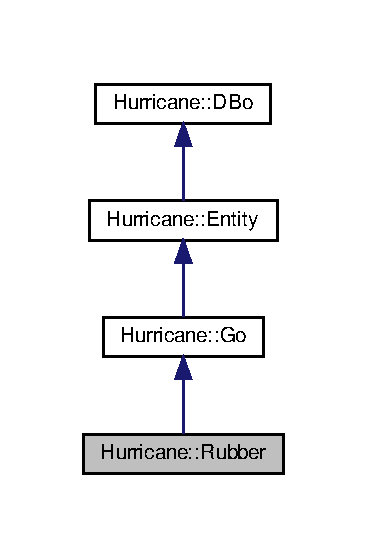
\includegraphics[width=176pt]{classHurricane_1_1Rubber__inherit__graph}
\end{center}
\end{figure}
\doxysubsection*{Public Types}
\begin{DoxyCompactItemize}
\item 
typedef \mbox{\hyperlink{classHurricane_1_1Go}{Go}} \mbox{\hyperlink{classHurricane_1_1Rubber_aa74649cee7cda714020e77194af2210a}{Inherit}}
\end{DoxyCompactItemize}
\doxysubsection*{Public Member Functions}
\begin{DoxyCompactItemize}
\item 
\mbox{\hyperlink{classHurricane_1_1Net}{Net}} $\ast$ \mbox{\hyperlink{classHurricane_1_1Rubber_a3d4156388d0a9e53daa00cdae9732e12}{get\+Net}} () const
\item 
\mbox{\hyperlink{classHurricane_1_1Hook}{Hook}} $\ast$ \mbox{\hyperlink{classHurricane_1_1Rubber_a9f7b9bc21b4df4c2bac602f045477711}{get\+Hook}} () const
\item 
unsigned \mbox{\hyperlink{classHurricane_1_1Rubber_a5fbe74e46313c0c1a264f0c7bda11e94}{get\+Count}} () const
\item 
\mbox{\hyperlink{classHurricane_1_1Point}{Point}} \mbox{\hyperlink{classHurricane_1_1Rubber_a124ef92401fd95ff794e381acd24e4ff}{get\+Center}} () const
\item 
\mbox{\hyperlink{namespaceHurricane_a9dcd9b74dc5e2b51bec7a13c25807e02}{Hooks}} \mbox{\hyperlink{classHurricane_1_1Rubber_a6d87ff89d80fbaeeb6fea4157b92d1e3}{get\+Hooks}} () const
\end{DoxyCompactItemize}
\doxysubsection*{Additional Inherited Members}


\doxysubsection{Detailed Description}
\mbox{\hyperlink{classHurricane_1_1Rubber}{Rubber}} description ({\bfseries{API}}) 

\hypertarget{classHurricane_1_1Rubber_secRubberIntro}{}\doxysubsection{Introduction}\label{classHurricane_1_1Rubber_secRubberIntro}
Ring introduce the concept of virtual connection between different master hooks present in the ring. \mbox{\hyperlink{classHurricane_1_1Rubber}{Rubber}} is just introduced to materialize this implicit relation.\hypertarget{classHurricane_1_1Rubber_secRubberConstructors}{}\doxysubsection{Constructors \& Destructors}\label{classHurricane_1_1Rubber_secRubberConstructors}
Rubbers are entirely managed by \mbox{\hyperlink{namespaceHurricane}{Hurricane}}. So no constructors nor destructor are avalaible. 

\doxysubsection{Member Typedef Documentation}
\mbox{\Hypertarget{classHurricane_1_1Rubber_aa74649cee7cda714020e77194af2210a}\label{classHurricane_1_1Rubber_aa74649cee7cda714020e77194af2210a}} 
\index{Hurricane::Rubber@{Hurricane::Rubber}!Inherit@{Inherit}}
\index{Inherit@{Inherit}!Hurricane::Rubber@{Hurricane::Rubber}}
\doxysubsubsection{\texorpdfstring{Inherit}{Inherit}}
{\footnotesize\ttfamily \mbox{\hyperlink{classHurricane_1_1Rubber_aa74649cee7cda714020e77194af2210a}{Hurricane\+::\+Rubber\+::\+Inherit}}}

Useful for calling upon methods of the base class without knowing it. 

\doxysubsection{Member Function Documentation}
\mbox{\Hypertarget{classHurricane_1_1Rubber_a3d4156388d0a9e53daa00cdae9732e12}\label{classHurricane_1_1Rubber_a3d4156388d0a9e53daa00cdae9732e12}} 
\index{Hurricane::Rubber@{Hurricane::Rubber}!getNet@{getNet}}
\index{getNet@{getNet}!Hurricane::Rubber@{Hurricane::Rubber}}
\doxysubsubsection{\texorpdfstring{getNet()}{getNet()}}
{\footnotesize\ttfamily \mbox{\hyperlink{classHurricane_1_1Net}{Net}} $\ast$ Hurricane\+::\+Rubber\+::get\+Net (\begin{DoxyParamCaption}{ }\end{DoxyParamCaption}) const\hspace{0.3cm}{\ttfamily [inline]}}

{\bfseries{Returns\+:}} the net owning the rubber. \mbox{\Hypertarget{classHurricane_1_1Rubber_a9f7b9bc21b4df4c2bac602f045477711}\label{classHurricane_1_1Rubber_a9f7b9bc21b4df4c2bac602f045477711}} 
\index{Hurricane::Rubber@{Hurricane::Rubber}!getHook@{getHook}}
\index{getHook@{getHook}!Hurricane::Rubber@{Hurricane::Rubber}}
\doxysubsubsection{\texorpdfstring{getHook()}{getHook()}}
{\footnotesize\ttfamily \mbox{\hyperlink{classHurricane_1_1Hook}{Hook}} $\ast$ Hurricane\+::\+Rubber\+::get\+Hook (\begin{DoxyParamCaption}{ }\end{DoxyParamCaption}) const\hspace{0.3cm}{\ttfamily [inline]}}

{\bfseries{Returns\+:}} one hook (necessarily a master hook) of the ring which has created the rubber. \mbox{\Hypertarget{classHurricane_1_1Rubber_a5fbe74e46313c0c1a264f0c7bda11e94}\label{classHurricane_1_1Rubber_a5fbe74e46313c0c1a264f0c7bda11e94}} 
\index{Hurricane::Rubber@{Hurricane::Rubber}!getCount@{getCount}}
\index{getCount@{getCount}!Hurricane::Rubber@{Hurricane::Rubber}}
\doxysubsubsection{\texorpdfstring{getCount()}{getCount()}}
{\footnotesize\ttfamily unsigned Hurricane\+::\+Rubber\+::get\+Count (\begin{DoxyParamCaption}{ }\end{DoxyParamCaption}) const\hspace{0.3cm}{\ttfamily [inline]}}

{\bfseries{Returns\+:}} the count associated to the rubber (in fact the number of master hooks of the ring).

\begin{DoxyRemark}{Remarks}
This count is at least equal to two else the rubber doesn\textquotesingle{}t exists (no need). 
\end{DoxyRemark}
\mbox{\Hypertarget{classHurricane_1_1Rubber_a124ef92401fd95ff794e381acd24e4ff}\label{classHurricane_1_1Rubber_a124ef92401fd95ff794e381acd24e4ff}} 
\index{Hurricane::Rubber@{Hurricane::Rubber}!getCenter@{getCenter}}
\index{getCenter@{getCenter}!Hurricane::Rubber@{Hurricane::Rubber}}
\doxysubsubsection{\texorpdfstring{getCenter()}{getCenter()}}
{\footnotesize\ttfamily \mbox{\hyperlink{classHurricane_1_1Point}{Point}} Hurricane\+::\+Rubber\+::get\+Center (\begin{DoxyParamCaption}{ }\end{DoxyParamCaption}) const}

{\bfseries{Returns\+:}} the center of the rubber (computed at the fly). \mbox{\Hypertarget{classHurricane_1_1Rubber_a6d87ff89d80fbaeeb6fea4157b92d1e3}\label{classHurricane_1_1Rubber_a6d87ff89d80fbaeeb6fea4157b92d1e3}} 
\index{Hurricane::Rubber@{Hurricane::Rubber}!getHooks@{getHooks}}
\index{getHooks@{getHooks}!Hurricane::Rubber@{Hurricane::Rubber}}
\doxysubsubsection{\texorpdfstring{getHooks()}{getHooks()}}
{\footnotesize\ttfamily \mbox{\hyperlink{namespaceHurricane_a9dcd9b74dc5e2b51bec7a13c25807e02}{Hooks}} Hurricane\+::\+Rubber\+::get\+Hooks (\begin{DoxyParamCaption}{ }\end{DoxyParamCaption}) const}

{\bfseries{Returns\+:}} the collection of master hooks that the rubber virtualy connect. 

The documentation for this class was generated from the following files\+:\begin{DoxyCompactItemize}
\item 
Rubber.\+h\item 
Rubber.\+dox\end{DoxyCompactItemize}

\hypertarget{classHurricane_1_1Segment}{}\doxysection{Hurricane\+::Segment Class Reference}
\label{classHurricane_1_1Segment}\index{Hurricane::Segment@{Hurricane::Segment}}


\mbox{\hyperlink{classHurricane_1_1Segment}{Segment}} description ({\bfseries{API}})  




Inheritance diagram for Hurricane\+::Segment\+:\nopagebreak
\begin{figure}[H]
\begin{center}
\leavevmode
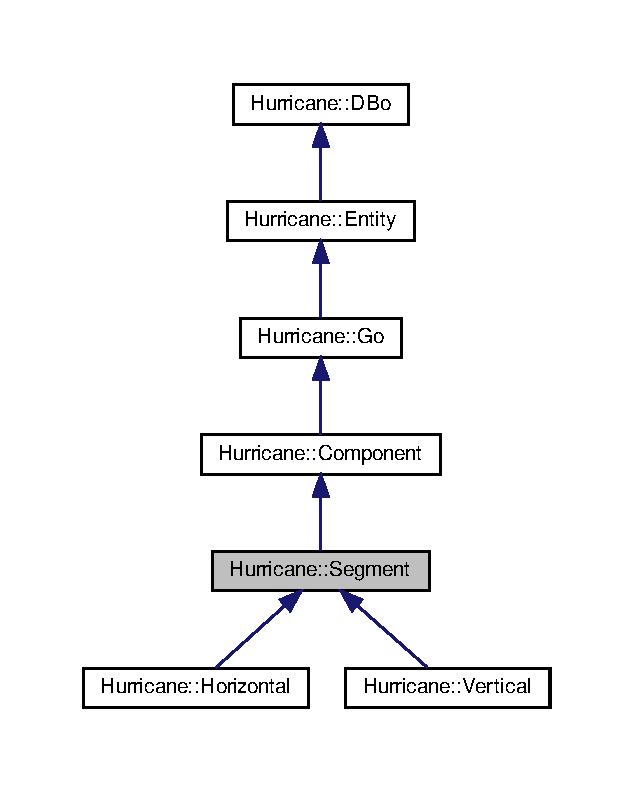
\includegraphics[width=304pt]{classHurricane_1_1Segment__inherit__graph}
\end{center}
\end{figure}
\doxysubsection*{Classes}
\begin{DoxyCompactItemize}
\item 
class \mbox{\hyperlink{classHurricane_1_1Segment_1_1SourceHook}{Source\+Hook}}
\item 
class \mbox{\hyperlink{classHurricane_1_1Segment_1_1TargetHook}{Target\+Hook}}
\end{DoxyCompactItemize}
\doxysubsection*{Public Types}
\begin{DoxyCompactItemize}
\item 
typedef \mbox{\hyperlink{classHurricane_1_1Component}{Component}} \mbox{\hyperlink{classHurricane_1_1Segment_a2f616ba119bb6e9751659814bdbf0320}{Inherit}}
\end{DoxyCompactItemize}
\doxysubsection*{Public Member Functions}
\begin{DoxyCompactItemize}
\item 
\mbox{\hyperlink{classHurricane_1_1Hook}{Hook}} $\ast$ \mbox{\hyperlink{classHurricane_1_1Segment_aa9d0303b444b44d7b8e47d42ac7151eb}{get\+Source\+Hook}} ()
\item 
\mbox{\hyperlink{classHurricane_1_1Hook}{Hook}} $\ast$ \mbox{\hyperlink{classHurricane_1_1Segment_a0fe6cd20516eca2a0b5639ab886bd831}{get\+Target\+Hook}} ()
\item 
\mbox{\hyperlink{classHurricane_1_1Hook}{Hook}} $\ast$ \mbox{\hyperlink{classHurricane_1_1Segment_afcd8471a2f2cfaa0e8e78a84ff7c09fc}{get\+Opposite\+Hook}} (const \mbox{\hyperlink{classHurricane_1_1Hook}{Hook}} $\ast$hook) const
\item 
\mbox{\hyperlink{classHurricane_1_1Component}{Component}} $\ast$ \mbox{\hyperlink{classHurricane_1_1Segment_aaa8954fc5948f2a881cdbc9213f9f7a9}{get\+Source}} () const
\item 
\mbox{\hyperlink{classHurricane_1_1Component}{Component}} $\ast$ \mbox{\hyperlink{classHurricane_1_1Segment_a1f7f13b33be3b1a20ea23b3f501296e9}{get\+Target}} () const
\item 
\mbox{\hyperlink{namespaceHurricane_a7d26d99aeb5dd6d70d51bd35d2473e72}{Components}} \mbox{\hyperlink{classHurricane_1_1Segment_ac179f0263fee7fc71e03c9cf8c2d4e45}{get\+Anchors}} () const
\item 
\mbox{\hyperlink{classHurricane_1_1Component}{Component}} $\ast$ \mbox{\hyperlink{classHurricane_1_1Segment_aa425757f271df5c58b024b0494c21588}{get\+Opposite\+Anchor}} (\mbox{\hyperlink{classHurricane_1_1Component}{Component}} $\ast$anchor) const
\item 
const \mbox{\hyperlink{classHurricane_1_1DbU_a4fbfa3e8c89347af76c9628ea06c4146}{Db\+U\+::\+Unit}} \& \mbox{\hyperlink{classHurricane_1_1Segment_a36c7ddda39077385bd8747a8c1df726a}{get\+Width}} () const
\item 
\mbox{\hyperlink{classHurricane_1_1DbU_a4fbfa3e8c89347af76c9628ea06c4146}{Db\+U\+::\+Unit}} \mbox{\hyperlink{classHurricane_1_1Segment_a58e4abcf545ad5c89ca2854a2b4471f8}{get\+Half\+Width}} () const
\item 
virtual \mbox{\hyperlink{classHurricane_1_1DbU_a4fbfa3e8c89347af76c9628ea06c4146}{Db\+U\+::\+Unit}} \mbox{\hyperlink{classHurricane_1_1Segment_a0347e3bde8e2e90b05cffdaf2d048710}{get\+SourceX}} () const =0
\item 
virtual \mbox{\hyperlink{classHurricane_1_1DbU_a4fbfa3e8c89347af76c9628ea06c4146}{Db\+U\+::\+Unit}} \mbox{\hyperlink{classHurricane_1_1Segment_abf305dd4510de6fe6fae5286acbe285a}{get\+SourceY}} () const =0
\item 
virtual \mbox{\hyperlink{classHurricane_1_1Point}{Point}} \mbox{\hyperlink{classHurricane_1_1Segment_a41c4b88c35b9af0ad741205d0a8ea9c2}{get\+Source\+Position}} () const
\item 
virtual \mbox{\hyperlink{classHurricane_1_1DbU_a4fbfa3e8c89347af76c9628ea06c4146}{Db\+U\+::\+Unit}} \mbox{\hyperlink{classHurricane_1_1Segment_abba6713e109a0925c078a9785274f389}{get\+TargetX}} () const =0
\item 
virtual \mbox{\hyperlink{classHurricane_1_1DbU_a4fbfa3e8c89347af76c9628ea06c4146}{Db\+U\+::\+Unit}} \mbox{\hyperlink{classHurricane_1_1Segment_a27d530abcff9742b81c4b549db161b90}{get\+TargetY}} () const =0
\item 
virtual \mbox{\hyperlink{classHurricane_1_1Point}{Point}} \mbox{\hyperlink{classHurricane_1_1Segment_af24bee306be3461bb5dd1ba680f2a2df}{get\+Target\+Position}} () const
\item 
virtual \mbox{\hyperlink{classHurricane_1_1DbU_a4fbfa3e8c89347af76c9628ea06c4146}{Db\+U\+::\+Unit}} \mbox{\hyperlink{classHurricane_1_1Segment_a9f6c42c2de0330aa6a486cdbf550cea1}{get\+Length}} () const =0
\item 
void \mbox{\hyperlink{classHurricane_1_1Segment_acd0b0cd25c824ba7f3b1ff2776c97cf1}{set\+Layer}} (const \mbox{\hyperlink{classHurricane_1_1Layer}{Layer}} $\ast$layer)
\item 
void \mbox{\hyperlink{classHurricane_1_1Segment_aec203d5d3aa96150979ba532d4bd1c7d}{set\+Width}} (const \mbox{\hyperlink{classHurricane_1_1DbU_a4fbfa3e8c89347af76c9628ea06c4146}{Db\+U\+::\+Unit}} \&width)
\item 
void \mbox{\hyperlink{classHurricane_1_1Segment_aceaa61242eb7275cf9c6a39cf1868c53}{invert}} ()
\end{DoxyCompactItemize}
\doxysubsection*{Additional Inherited Members}


\doxysubsection{Detailed Description}
\mbox{\hyperlink{classHurricane_1_1Segment}{Segment}} description ({\bfseries{API}}) 

\hypertarget{classHurricane_1_1Segment_secSegmentIntro}{}\doxysubsection{Introduction}\label{classHurricane_1_1Segment_secSegmentIntro}
Segments are abstract objects introducing the concept of link between two components.

They are implicitely oriented, but that doesn\textquotesingle{}t represent any particular signification (for layout objects at least). 

\doxysubsection{Member Typedef Documentation}
\mbox{\Hypertarget{classHurricane_1_1Segment_a2f616ba119bb6e9751659814bdbf0320}\label{classHurricane_1_1Segment_a2f616ba119bb6e9751659814bdbf0320}} 
\index{Hurricane::Segment@{Hurricane::Segment}!Inherit@{Inherit}}
\index{Inherit@{Inherit}!Hurricane::Segment@{Hurricane::Segment}}
\doxysubsubsection{\texorpdfstring{Inherit}{Inherit}}
{\footnotesize\ttfamily \mbox{\hyperlink{classHurricane_1_1Segment_a2f616ba119bb6e9751659814bdbf0320}{Hurricane\+::\+Segment\+::\+Inherit}}}

Useful for calling upon methods of the base class without knowing it. 

\doxysubsection{Member Function Documentation}
\mbox{\Hypertarget{classHurricane_1_1Segment_aa9d0303b444b44d7b8e47d42ac7151eb}\label{classHurricane_1_1Segment_aa9d0303b444b44d7b8e47d42ac7151eb}} 
\index{Hurricane::Segment@{Hurricane::Segment}!getSourceHook@{getSourceHook}}
\index{getSourceHook@{getSourceHook}!Hurricane::Segment@{Hurricane::Segment}}
\doxysubsubsection{\texorpdfstring{getSourceHook()}{getSourceHook()}}
{\footnotesize\ttfamily \mbox{\hyperlink{classHurricane_1_1Segment_1_1SourceHook}{Segment\+::\+Source\+Hook}} $\ast$ Hurricane\+::\+Segment\+::get\+Source\+Hook (\begin{DoxyParamCaption}{ }\end{DoxyParamCaption})\hspace{0.3cm}{\ttfamily [inline]}}

{\bfseries{Returns\+:}} the hook through which the segment origin can be anchored on a component. \mbox{\Hypertarget{classHurricane_1_1Segment_a0fe6cd20516eca2a0b5639ab886bd831}\label{classHurricane_1_1Segment_a0fe6cd20516eca2a0b5639ab886bd831}} 
\index{Hurricane::Segment@{Hurricane::Segment}!getTargetHook@{getTargetHook}}
\index{getTargetHook@{getTargetHook}!Hurricane::Segment@{Hurricane::Segment}}
\doxysubsubsection{\texorpdfstring{getTargetHook()}{getTargetHook()}}
{\footnotesize\ttfamily \mbox{\hyperlink{classHurricane_1_1Segment_1_1TargetHook}{Segment\+::\+Target\+Hook}} $\ast$ Hurricane\+::\+Segment\+::get\+Target\+Hook (\begin{DoxyParamCaption}{ }\end{DoxyParamCaption})\hspace{0.3cm}{\ttfamily [inline]}}

{\bfseries{Returns\+:}} the hook through which the segment extremity can be anchored on a component. \mbox{\Hypertarget{classHurricane_1_1Segment_afcd8471a2f2cfaa0e8e78a84ff7c09fc}\label{classHurricane_1_1Segment_afcd8471a2f2cfaa0e8e78a84ff7c09fc}} 
\index{Hurricane::Segment@{Hurricane::Segment}!getOppositeHook@{getOppositeHook}}
\index{getOppositeHook@{getOppositeHook}!Hurricane::Segment@{Hurricane::Segment}}
\doxysubsubsection{\texorpdfstring{getOppositeHook()}{getOppositeHook()}}
{\footnotesize\ttfamily \mbox{\hyperlink{classHurricane_1_1Hook}{Hook}} $\ast$ Hurricane\+::\+Segment\+::get\+Opposite\+Hook (\begin{DoxyParamCaption}\item[{const \mbox{\hyperlink{classHurricane_1_1Hook}{Hook}} $\ast$}]{hook }\end{DoxyParamCaption}) const}

{\bfseries{Returns\+:}} the target hook of the segment if {\ttfamily $<$hook$>$} is the source hook of the segment.

{\bfseries{Returns\+:}} the source hook of the segment if {\ttfamily $<$hook$>$} is the target hook of the segment.

{\bfseries{Returns\+:}} NULL otherwise. \mbox{\Hypertarget{classHurricane_1_1Segment_aaa8954fc5948f2a881cdbc9213f9f7a9}\label{classHurricane_1_1Segment_aaa8954fc5948f2a881cdbc9213f9f7a9}} 
\index{Hurricane::Segment@{Hurricane::Segment}!getSource@{getSource}}
\index{getSource@{getSource}!Hurricane::Segment@{Hurricane::Segment}}
\doxysubsubsection{\texorpdfstring{getSource()}{getSource()}}
{\footnotesize\ttfamily \mbox{\hyperlink{classHurricane_1_1Component}{Component}} $\ast$ Hurricane\+::\+Segment\+::get\+Source (\begin{DoxyParamCaption}{ }\end{DoxyParamCaption}) const}

The source hook being a slave one, it may have an associated master hook representing the body of the component on wich the segment origin is anchored.

So, this method returns the component owner of this master hook, if any, else a NULL pointer. \mbox{\Hypertarget{classHurricane_1_1Segment_a1f7f13b33be3b1a20ea23b3f501296e9}\label{classHurricane_1_1Segment_a1f7f13b33be3b1a20ea23b3f501296e9}} 
\index{Hurricane::Segment@{Hurricane::Segment}!getTarget@{getTarget}}
\index{getTarget@{getTarget}!Hurricane::Segment@{Hurricane::Segment}}
\doxysubsubsection{\texorpdfstring{getTarget()}{getTarget()}}
{\footnotesize\ttfamily \mbox{\hyperlink{classHurricane_1_1Component}{Component}} $\ast$ Hurricane\+::\+Segment\+::get\+Target (\begin{DoxyParamCaption}{ }\end{DoxyParamCaption}) const}

The target hook being a slave one, it may have an associated master hook representing the body of the component on wich the segment extremity is anchored.

So, this method returns the component owner of this master hook, if any, else a NULL pointer. \mbox{\Hypertarget{classHurricane_1_1Segment_ac179f0263fee7fc71e03c9cf8c2d4e45}\label{classHurricane_1_1Segment_ac179f0263fee7fc71e03c9cf8c2d4e45}} 
\index{Hurricane::Segment@{Hurricane::Segment}!getAnchors@{getAnchors}}
\index{getAnchors@{getAnchors}!Hurricane::Segment@{Hurricane::Segment}}
\doxysubsubsection{\texorpdfstring{getAnchors()}{getAnchors()}}
{\footnotesize\ttfamily \mbox{\hyperlink{namespaceHurricane_a7d26d99aeb5dd6d70d51bd35d2473e72}{Components}} Hurricane\+::\+Segment\+::get\+Anchors (\begin{DoxyParamCaption}{ }\end{DoxyParamCaption}) const}

{\bfseries{Returns\+:}} the collection of anchors. This collection is composed by the source (if non NULL) and the target (if non NULL) of the segment (may be empty if all extremities of the segment aren\textquotesingle{}t anchored). \mbox{\Hypertarget{classHurricane_1_1Segment_aa425757f271df5c58b024b0494c21588}\label{classHurricane_1_1Segment_aa425757f271df5c58b024b0494c21588}} 
\index{Hurricane::Segment@{Hurricane::Segment}!getOppositeAnchor@{getOppositeAnchor}}
\index{getOppositeAnchor@{getOppositeAnchor}!Hurricane::Segment@{Hurricane::Segment}}
\doxysubsubsection{\texorpdfstring{getOppositeAnchor()}{getOppositeAnchor()}}
{\footnotesize\ttfamily \mbox{\hyperlink{classHurricane_1_1Component}{Component}} $\ast$ Hurricane\+::\+Segment\+::get\+Opposite\+Anchor (\begin{DoxyParamCaption}\item[{\mbox{\hyperlink{classHurricane_1_1Component}{Component}} $\ast$}]{anchor }\end{DoxyParamCaption}) const}

{\bfseries{Returns\+:}} the target anchor of the segment if {\ttfamily $<$anchor$>$} is the source anchor of the segment (may be NULL)

{\bfseries{Returns\+:}} the source anchor of the segment if {\ttfamily $<$anchor$>$} is the target anchor of the segment (may be NULL)

{\bfseries{Returns\+:}} NULL otherwise. \mbox{\Hypertarget{classHurricane_1_1Segment_a36c7ddda39077385bd8747a8c1df726a}\label{classHurricane_1_1Segment_a36c7ddda39077385bd8747a8c1df726a}} 
\index{Hurricane::Segment@{Hurricane::Segment}!getWidth@{getWidth}}
\index{getWidth@{getWidth}!Hurricane::Segment@{Hurricane::Segment}}
\doxysubsubsection{\texorpdfstring{getWidth()}{getWidth()}}
{\footnotesize\ttfamily const \mbox{\hyperlink{classHurricane_1_1DbU_a4fbfa3e8c89347af76c9628ea06c4146}{Db\+U\+::\+Unit}} \& Hurricane\+::\+Segment\+::get\+Width (\begin{DoxyParamCaption}{ }\end{DoxyParamCaption}) const\hspace{0.3cm}{\ttfamily [inline]}}

{\bfseries{Returns\+:}} the segment width. \mbox{\Hypertarget{classHurricane_1_1Segment_a58e4abcf545ad5c89ca2854a2b4471f8}\label{classHurricane_1_1Segment_a58e4abcf545ad5c89ca2854a2b4471f8}} 
\index{Hurricane::Segment@{Hurricane::Segment}!getHalfWidth@{getHalfWidth}}
\index{getHalfWidth@{getHalfWidth}!Hurricane::Segment@{Hurricane::Segment}}
\doxysubsubsection{\texorpdfstring{getHalfWidth()}{getHalfWidth()}}
{\footnotesize\ttfamily \mbox{\hyperlink{classHurricane_1_1DbU_a4fbfa3e8c89347af76c9628ea06c4146}{Db\+U\+::\+Unit}} Hurricane\+::\+Segment\+::get\+Half\+Width (\begin{DoxyParamCaption}{ }\end{DoxyParamCaption}) const\hspace{0.3cm}{\ttfamily [inline]}}

{\bfseries{Returns\+:}} the segment half width. \mbox{\Hypertarget{classHurricane_1_1Segment_a0347e3bde8e2e90b05cffdaf2d048710}\label{classHurricane_1_1Segment_a0347e3bde8e2e90b05cffdaf2d048710}} 
\index{Hurricane::Segment@{Hurricane::Segment}!getSourceX@{getSourceX}}
\index{getSourceX@{getSourceX}!Hurricane::Segment@{Hurricane::Segment}}
\doxysubsubsection{\texorpdfstring{getSourceX()}{getSourceX()}}
{\footnotesize\ttfamily \mbox{\hyperlink{classHurricane_1_1DbU_a4fbfa3e8c89347af76c9628ea06c4146}{Db\+U\+::\+Unit}} Hurricane\+::\+Segment\+::get\+SourceX (\begin{DoxyParamCaption}{ }\end{DoxyParamCaption}) const\hspace{0.3cm}{\ttfamily [pure virtual]}}

{\bfseries{Returns\+:}} the abscissa of the segment origin. \mbox{\Hypertarget{classHurricane_1_1Segment_abf305dd4510de6fe6fae5286acbe285a}\label{classHurricane_1_1Segment_abf305dd4510de6fe6fae5286acbe285a}} 
\index{Hurricane::Segment@{Hurricane::Segment}!getSourceY@{getSourceY}}
\index{getSourceY@{getSourceY}!Hurricane::Segment@{Hurricane::Segment}}
\doxysubsubsection{\texorpdfstring{getSourceY()}{getSourceY()}}
{\footnotesize\ttfamily \mbox{\hyperlink{classHurricane_1_1DbU_a4fbfa3e8c89347af76c9628ea06c4146}{Db\+U\+::\+Unit}} Hurricane\+::\+Segment\+::get\+SourceY (\begin{DoxyParamCaption}{ }\end{DoxyParamCaption}) const\hspace{0.3cm}{\ttfamily [pure virtual]}}

{\bfseries{Returns\+:}} the ordinate of the segment origin. \mbox{\Hypertarget{classHurricane_1_1Segment_a41c4b88c35b9af0ad741205d0a8ea9c2}\label{classHurricane_1_1Segment_a41c4b88c35b9af0ad741205d0a8ea9c2}} 
\index{Hurricane::Segment@{Hurricane::Segment}!getSourcePosition@{getSourcePosition}}
\index{getSourcePosition@{getSourcePosition}!Hurricane::Segment@{Hurricane::Segment}}
\doxysubsubsection{\texorpdfstring{getSourcePosition()}{getSourcePosition()}}
{\footnotesize\ttfamily \mbox{\hyperlink{classHurricane_1_1Point}{Point}} Hurricane\+::\+Segment\+::get\+Source\+Position (\begin{DoxyParamCaption}{ }\end{DoxyParamCaption}) const\hspace{0.3cm}{\ttfamily [virtual]}}

{\bfseries{Returns\+:}} the point location of the segment origin. \mbox{\Hypertarget{classHurricane_1_1Segment_abba6713e109a0925c078a9785274f389}\label{classHurricane_1_1Segment_abba6713e109a0925c078a9785274f389}} 
\index{Hurricane::Segment@{Hurricane::Segment}!getTargetX@{getTargetX}}
\index{getTargetX@{getTargetX}!Hurricane::Segment@{Hurricane::Segment}}
\doxysubsubsection{\texorpdfstring{getTargetX()}{getTargetX()}}
{\footnotesize\ttfamily \mbox{\hyperlink{classHurricane_1_1DbU_a4fbfa3e8c89347af76c9628ea06c4146}{Db\+U\+::\+Unit}} Hurricane\+::\+Segment\+::get\+TargetX (\begin{DoxyParamCaption}{ }\end{DoxyParamCaption}) const\hspace{0.3cm}{\ttfamily [pure virtual]}}

{\bfseries{Returns\+:}} the abscissa of the segment extremity. \mbox{\Hypertarget{classHurricane_1_1Segment_a27d530abcff9742b81c4b549db161b90}\label{classHurricane_1_1Segment_a27d530abcff9742b81c4b549db161b90}} 
\index{Hurricane::Segment@{Hurricane::Segment}!getTargetY@{getTargetY}}
\index{getTargetY@{getTargetY}!Hurricane::Segment@{Hurricane::Segment}}
\doxysubsubsection{\texorpdfstring{getTargetY()}{getTargetY()}}
{\footnotesize\ttfamily \mbox{\hyperlink{classHurricane_1_1DbU_a4fbfa3e8c89347af76c9628ea06c4146}{Db\+U\+::\+Unit}} Hurricane\+::\+Segment\+::get\+TargetY (\begin{DoxyParamCaption}{ }\end{DoxyParamCaption}) const\hspace{0.3cm}{\ttfamily [pure virtual]}}

{\bfseries{Returns\+:}} the ordinate of the segment extremity. \mbox{\Hypertarget{classHurricane_1_1Segment_af24bee306be3461bb5dd1ba680f2a2df}\label{classHurricane_1_1Segment_af24bee306be3461bb5dd1ba680f2a2df}} 
\index{Hurricane::Segment@{Hurricane::Segment}!getTargetPosition@{getTargetPosition}}
\index{getTargetPosition@{getTargetPosition}!Hurricane::Segment@{Hurricane::Segment}}
\doxysubsubsection{\texorpdfstring{getTargetPosition()}{getTargetPosition()}}
{\footnotesize\ttfamily \mbox{\hyperlink{classHurricane_1_1Point}{Point}} Hurricane\+::\+Segment\+::get\+Target\+Position (\begin{DoxyParamCaption}{ }\end{DoxyParamCaption}) const\hspace{0.3cm}{\ttfamily [virtual]}}

{\bfseries{Returns\+:}} the point location of the segment extremity. \mbox{\Hypertarget{classHurricane_1_1Segment_a9f6c42c2de0330aa6a486cdbf550cea1}\label{classHurricane_1_1Segment_a9f6c42c2de0330aa6a486cdbf550cea1}} 
\index{Hurricane::Segment@{Hurricane::Segment}!getLength@{getLength}}
\index{getLength@{getLength}!Hurricane::Segment@{Hurricane::Segment}}
\doxysubsubsection{\texorpdfstring{getLength()}{getLength()}}
{\footnotesize\ttfamily \mbox{\hyperlink{classHurricane_1_1DbU_a4fbfa3e8c89347af76c9628ea06c4146}{Db\+U\+::\+Unit}} Hurricane\+::\+Segment\+::get\+Length (\begin{DoxyParamCaption}{ }\end{DoxyParamCaption}) const\hspace{0.3cm}{\ttfamily [pure virtual]}}

{\bfseries{Returns\+:}} the segment length. \mbox{\Hypertarget{classHurricane_1_1Segment_acd0b0cd25c824ba7f3b1ff2776c97cf1}\label{classHurricane_1_1Segment_acd0b0cd25c824ba7f3b1ff2776c97cf1}} 
\index{Hurricane::Segment@{Hurricane::Segment}!setLayer@{setLayer}}
\index{setLayer@{setLayer}!Hurricane::Segment@{Hurricane::Segment}}
\doxysubsubsection{\texorpdfstring{setLayer()}{setLayer()}}
{\footnotesize\ttfamily void Hurricane\+::\+Segment\+::set\+Layer (\begin{DoxyParamCaption}\item[{const \mbox{\hyperlink{classHurricane_1_1Layer}{Layer}} $\ast$}]{layer }\end{DoxyParamCaption})}

sets the segment layer. \mbox{\Hypertarget{classHurricane_1_1Segment_aec203d5d3aa96150979ba532d4bd1c7d}\label{classHurricane_1_1Segment_aec203d5d3aa96150979ba532d4bd1c7d}} 
\index{Hurricane::Segment@{Hurricane::Segment}!setWidth@{setWidth}}
\index{setWidth@{setWidth}!Hurricane::Segment@{Hurricane::Segment}}
\doxysubsubsection{\texorpdfstring{setWidth()}{setWidth()}}
{\footnotesize\ttfamily void Hurricane\+::\+Segment\+::set\+Width (\begin{DoxyParamCaption}\item[{const \mbox{\hyperlink{classHurricane_1_1DbU_a4fbfa3e8c89347af76c9628ea06c4146}{Db\+U\+::\+Unit}} \&}]{width }\end{DoxyParamCaption})}

sets the segment width. \mbox{\Hypertarget{classHurricane_1_1Segment_aceaa61242eb7275cf9c6a39cf1868c53}\label{classHurricane_1_1Segment_aceaa61242eb7275cf9c6a39cf1868c53}} 
\index{Hurricane::Segment@{Hurricane::Segment}!invert@{invert}}
\index{invert@{invert}!Hurricane::Segment@{Hurricane::Segment}}
\doxysubsubsection{\texorpdfstring{invert()}{invert()}}
{\footnotesize\ttfamily void Hurricane\+::\+Segment\+::invert (\begin{DoxyParamCaption}{ }\end{DoxyParamCaption})}

invert the segment. The source and target of the segment are permutted. 

The documentation for this class was generated from the following files\+:\begin{DoxyCompactItemize}
\item 
Segment.\+h\item 
Segment.\+dox\end{DoxyCompactItemize}

\hypertarget{classHurricane_1_1SetCollection}{}\doxysection{Hurricane\+::Set\+Collection$<$ Element, Compare $>$ Class Template Reference}
\label{classHurricane_1_1SetCollection}\index{Hurricane::SetCollection$<$ Element, Compare $>$@{Hurricane::SetCollection$<$ Element, Compare $>$}}


\mbox{\hyperlink{namespaceHurricane}{Hurricane}} \mbox{\hyperlink{classHurricane_1_1Collection}{Collection}} wrapper around a std\+::set.  




Inheritance diagram for Hurricane\+::Set\+Collection$<$ Element, Compare $>$\+:\nopagebreak
\begin{figure}[H]
\begin{center}
\leavevmode
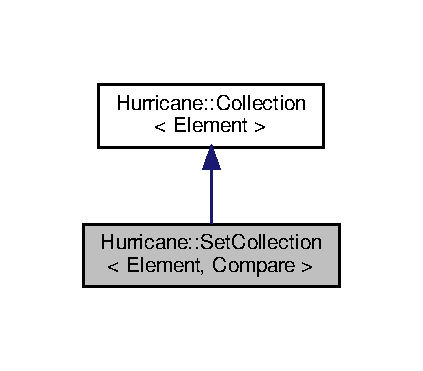
\includegraphics[width=203pt]{classHurricane_1_1SetCollection__inherit__graph}
\end{center}
\end{figure}
\doxysubsection*{Public Member Functions}
\begin{Indent}\textbf{ Collection Collection}\par
{\em \hypertarget{Collection_8h_secCollectionUtilitarians}{}\doxysubsection{Utilitarians}\label{Collection_8h_secCollectionUtilitarians}
{\bfseries{Collection\+::\+Fill}} {\bfseries{Collection\+::\+Fill}} {\bfseries{Collection\+::\+Fill}} \begin{DoxyRemark}{Remarks}
The elements are added to the container in the order with which the collection is visited. So the same order will appear in a list or a vector, but for a set they will be inserted according to the set ordering method. 
\end{DoxyRemark}
}\begin{DoxyCompactItemize}
\item 
\mbox{\hyperlink{classHurricane_1_1SetCollection_a3ee200fd00f3a6951906209c11c03e34}{Set\+Collection}} (const Element\+Set $\ast$element\+Set=NULL)
\end{DoxyCompactItemize}
\end{Indent}


\doxysubsection{Detailed Description}
\subsubsection*{template$<$class Element, class Compare = less$<$\+Element$>$$>$\newline
class Hurricane\+::\+Set\+Collection$<$ Element, Compare $>$}

\mbox{\hyperlink{namespaceHurricane}{Hurricane}} \mbox{\hyperlink{classHurricane_1_1Collection}{Collection}} wrapper around a std\+::set. 

Automatically wrap a \mbox{\hyperlink{namespaceHurricane}{Hurricane}} \mbox{\hyperlink{classHurricane_1_1Collection}{Collection}} around a stl\+::set. 

\doxysubsection{Constructor \& Destructor Documentation}
\mbox{\Hypertarget{classHurricane_1_1SetCollection_a3ee200fd00f3a6951906209c11c03e34}\label{classHurricane_1_1SetCollection_a3ee200fd00f3a6951906209c11c03e34}} 
\index{Hurricane::SetCollection$<$ Element, Compare $>$@{Hurricane::SetCollection$<$ Element, Compare $>$}!SetCollection@{SetCollection}}
\index{SetCollection@{SetCollection}!Hurricane::SetCollection$<$ Element, Compare $>$@{Hurricane::SetCollection$<$ Element, Compare $>$}}
\doxysubsubsection{\texorpdfstring{SetCollection()}{SetCollection()}}
{\footnotesize\ttfamily template$<$class Element , class Compare  = less$<$\+Element$>$$>$ \\
\mbox{\hyperlink{classHurricane_1_1SetCollection}{Hurricane\+::\+Set\+Collection}}$<$ Element, Compare $>$\+::\mbox{\hyperlink{classHurricane_1_1SetCollection}{Set\+Collection}} (\begin{DoxyParamCaption}\item[{const Element\+Set $\ast$}]{element\+Set = {\ttfamily NULL} }\end{DoxyParamCaption})\hspace{0.3cm}{\ttfamily [inline]}}

Constructor from a STL set, the set must not be de-\/allocated. 

The documentation for this class was generated from the following files\+:\begin{DoxyCompactItemize}
\item 
Set\+Collection.\+h\item 
Collection.\+dox\end{DoxyCompactItemize}

\hypertarget{classHurricane_1_1SharedProperty}{}\doxysection{Hurricane\+::Shared\+Property Class Reference}
\label{classHurricane_1_1SharedProperty}\index{Hurricane::SharedProperty@{Hurricane::SharedProperty}}


\mbox{\hyperlink{classHurricane_1_1SharedProperty}{Shared\+Property}} description ({\bfseries{API}})  




Inheritance diagram for Hurricane\+::Shared\+Property\+:\nopagebreak
\begin{figure}[H]
\begin{center}
\leavevmode
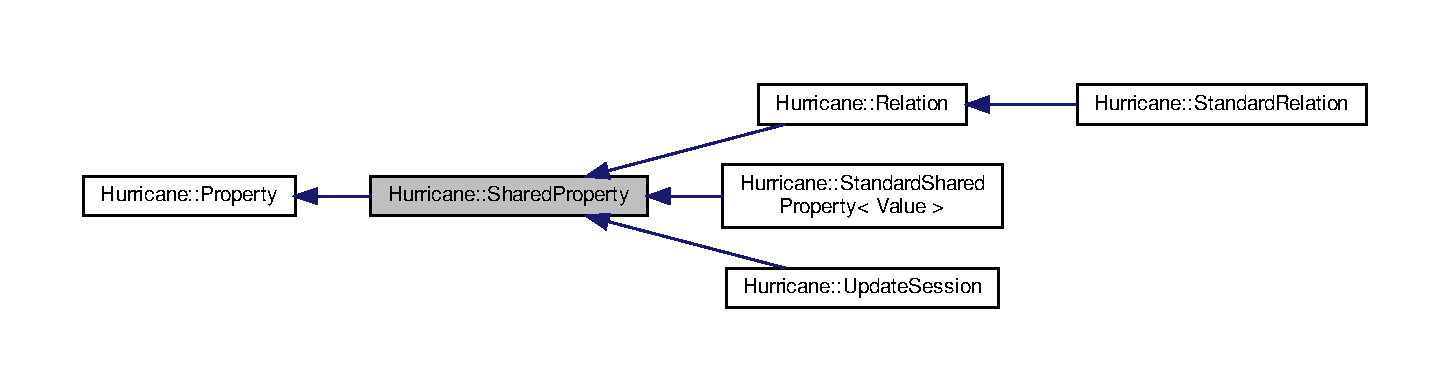
\includegraphics[width=350pt]{classHurricane_1_1SharedProperty__inherit__graph}
\end{center}
\end{figure}
\doxysubsection*{Additional Inherited Members}


\doxysubsection{Detailed Description}
\mbox{\hyperlink{classHurricane_1_1SharedProperty}{Shared\+Property}} description ({\bfseries{API}}) 

\hypertarget{classHurricane_1_1SharedProperty_secSharedPropertyIntro}{}\doxysubsection{Introduction}\label{classHurricane_1_1SharedProperty_secSharedPropertyIntro}
Shared properties can be attached to many objects of the data base.

When a new property is created, it is not yet assigned to any particular object. It becomes effectively the property of an object after the call {\bfseries{dbo-\/$>$Put(property)}}. The property then receives a message {\bfseries{On\+Captured\+By}} whose argument is the additional owner. From that time onwards, this object becomes partially responsible of the future of the property.

{\bfseries{What can happen then ?}}

If the property is destroyed \+: The property being shared, it informs its owners of its deletion. Each of those owners detaches it from the list of its properties. If the object is a quark and that property is the last one it owns, it automatically deletes itself.

If a property of same name already exist \+: Two properties with the same name can\textquotesingle{}t cohabit, the older one is released by the object which receives the message {\bfseries{On\+Released\+By}} from that old property and proceeds as required according to the type of property.

If the property is attached to a new owner \+: Being shared, the property is simply captured by this new owner.

If one of the owners of the property is destroyed \+: The properties captured by this object are then released. The future of those properties is here completely managed by the different messages {\bfseries{On\+Released\+By}} which are associated to them. If the deleted object is the last owner of a shared property, this one is automatically deleted. 

The documentation for this class was generated from the following file\+:\begin{DoxyCompactItemize}
\item 
Property.\+h\end{DoxyCompactItemize}

\hypertarget{classHurricane_1_1Slice}{}\section{Hurricane\+:\+:Slice Class Reference}
\label{classHurricane_1_1Slice}\index{Hurricane\+::\+Slice@{Hurricane\+::\+Slice}}


\mbox{\hyperlink{classHurricane_1_1Slice}{Slice}} description ({\bfseries A\+PI})  


\subsection*{Public Member Functions}
\begin{DoxyCompactItemize}
\item 
\mbox{\hyperlink{classHurricane_1_1Cell}{Cell}} $\ast$ \mbox{\hyperlink{classHurricane_1_1Slice_ae7a75f373a3d4e8878007c38688000f8}{get\+Cell}} () const
\item 
const \mbox{\hyperlink{classHurricane_1_1Layer}{Layer}} $\ast$ \mbox{\hyperlink{classHurricane_1_1Slice_a76c011cd461e588474a22fd0026e1f8f}{get\+Layer}} () const
\item 
const \mbox{\hyperlink{classHurricane_1_1Box}{Box}} \& \mbox{\hyperlink{classHurricane_1_1Slice_aa1a139b188879c37a8878a2353401d65}{get\+Bounding\+Box}} () const
\item 
\mbox{\hyperlink{namespaceHurricane_a4456a34f3bc6766d471c3064ace19759}{Gos}} \mbox{\hyperlink{classHurricane_1_1Slice_abc257f5b91c01c01a618787fd73db97b}{get\+Gos}} () const
\item 
\mbox{\hyperlink{namespaceHurricane_a7d26d99aeb5dd6d70d51bd35d2473e72}{Components}} \mbox{\hyperlink{classHurricane_1_1Slice_afe7c766d33e16461c3667af88e64773e}{get\+Components}} () const
\item 
\mbox{\hyperlink{namespaceHurricane_a7d26d99aeb5dd6d70d51bd35d2473e72}{Components}} \mbox{\hyperlink{classHurricane_1_1Slice_ada51a63690db8912eb58f1f33aa9f62c}{get\+Components\+Under}} (const \mbox{\hyperlink{classHurricane_1_1Box}{Box}} \&area, \mbox{\hyperlink{group__DbUGroup_ga4fbfa3e8c89347af76c9628ea06c4146}{Db\+U\+::\+Unit}} threshold=0) const
\end{DoxyCompactItemize}


\subsection{Detailed Description}
\mbox{\hyperlink{classHurricane_1_1Slice}{Slice}} description ({\bfseries A\+PI}) 

\hypertarget{classHurricane_1_1Slice_secSliceIntro}{}\subsection{Introduction}\label{classHurricane_1_1Slice_secSliceIntro}
The slices are objects which split the layout description of a cell into horizontal slices grouping all objects located on a given layer and storing them into a fast geometrical access structure implemented by a quadtree.\hypertarget{classHurricane_1_1Slice_secSliceConstructionAndDestruction}{}\subsection{Construction and destruction}\label{classHurricane_1_1Slice_secSliceConstructionAndDestruction}
The slices are fully managed by the cells \+: they are neither created nor destroyed by the application programmer.

Components are inserted in a slice (at their creation) and removed from their slice (at their deletion).

Empty slices being automatically deleted, you must never store pointers to them.\hypertarget{classHurricane_1_1Slice_secSliceExample}{}\subsection{Example}\label{classHurricane_1_1Slice_secSliceExample}
The following example shows how to visit all cell components lying on a given basic layer and whose bounding box intersects some rectangular area. 
\begin{DoxyCode}
Cell* cell = ...; \textcolor{comment}{// we get the cell}
 
BasicLayer* basicLayer = ...; \textcolor{comment}{// we get the basic layer}
 
Box area = ...; \textcolor{comment}{// we define the rectangular area}
 
forEach(Slice*, islice, cell->getSlices()) \{
  \textcolor{keywordflow}{if} (islice->getLayer()->contains(basicLayer)) \{
    forEach(Component*, icomponent, slice->getComponentsUnder(area)) \{
      \textcolor{comment}{// ...}
      \textcolor{comment}{// here we visit all requested components}
      \textcolor{comment}{// ...}
    \}
  \}
\}
\end{DoxyCode}
 

\subsection{Member Function Documentation}
\mbox{\Hypertarget{classHurricane_1_1Slice_ae7a75f373a3d4e8878007c38688000f8}\label{classHurricane_1_1Slice_ae7a75f373a3d4e8878007c38688000f8}} 
\index{Hurricane\+::\+Slice@{Hurricane\+::\+Slice}!get\+Cell@{get\+Cell}}
\index{get\+Cell@{get\+Cell}!Hurricane\+::\+Slice@{Hurricane\+::\+Slice}}
\subsubsection{\texorpdfstring{get\+Cell()}{getCell()}}
{\footnotesize\ttfamily \mbox{\hyperlink{classHurricane_1_1Cell}{Cell}} $\ast$ Hurricane\+::\+Slice\+::get\+Cell (\begin{DoxyParamCaption}{ }\end{DoxyParamCaption}) const\hspace{0.3cm}{\ttfamily [inline]}}

{\bfseries Returns\+:} the cell owning the slice. \mbox{\Hypertarget{classHurricane_1_1Slice_a76c011cd461e588474a22fd0026e1f8f}\label{classHurricane_1_1Slice_a76c011cd461e588474a22fd0026e1f8f}} 
\index{Hurricane\+::\+Slice@{Hurricane\+::\+Slice}!get\+Layer@{get\+Layer}}
\index{get\+Layer@{get\+Layer}!Hurricane\+::\+Slice@{Hurricane\+::\+Slice}}
\subsubsection{\texorpdfstring{get\+Layer()}{getLayer()}}
{\footnotesize\ttfamily \mbox{\hyperlink{classHurricane_1_1Layer}{Layer}} $\ast$ Hurricane\+::\+Slice\+::get\+Layer (\begin{DoxyParamCaption}{ }\end{DoxyParamCaption}) const\hspace{0.3cm}{\ttfamily [inline]}}

{\bfseries Returns\+:} the layer associated to the slice \+: all components lying in a cell are perforce located on that layer. \mbox{\Hypertarget{classHurricane_1_1Slice_aa1a139b188879c37a8878a2353401d65}\label{classHurricane_1_1Slice_aa1a139b188879c37a8878a2353401d65}} 
\index{Hurricane\+::\+Slice@{Hurricane\+::\+Slice}!get\+Bounding\+Box@{get\+Bounding\+Box}}
\index{get\+Bounding\+Box@{get\+Bounding\+Box}!Hurricane\+::\+Slice@{Hurricane\+::\+Slice}}
\subsubsection{\texorpdfstring{get\+Bounding\+Box()}{getBoundingBox()}}
{\footnotesize\ttfamily \mbox{\hyperlink{classHurricane_1_1Box}{Box}} Hurricane\+::\+Slice\+::get\+Bounding\+Box (\begin{DoxyParamCaption}{ }\end{DoxyParamCaption}) const\hspace{0.3cm}{\ttfamily [inline]}}

{\bfseries Returns\+:} the bounding box of the slice, that is the smallest enclosing rectangle of all its components. 

References Hurricane\+::\+Quad\+Tree\+::get\+Bounding\+Box().

\mbox{\Hypertarget{classHurricane_1_1Slice_abc257f5b91c01c01a618787fd73db97b}\label{classHurricane_1_1Slice_abc257f5b91c01c01a618787fd73db97b}} 
\index{Hurricane\+::\+Slice@{Hurricane\+::\+Slice}!get\+Gos@{get\+Gos}}
\index{get\+Gos@{get\+Gos}!Hurricane\+::\+Slice@{Hurricane\+::\+Slice}}
\subsubsection{\texorpdfstring{get\+Gos()}{getGos()}}
{\footnotesize\ttfamily const \mbox{\hyperlink{namespaceHurricane_a4456a34f3bc6766d471c3064ace19759}{Gos}} Hurricane\+::\+Slice\+::get\+Gos (\begin{DoxyParamCaption}{ }\end{DoxyParamCaption}) const\hspace{0.3cm}{\ttfamily [inline]}}

{\bfseries Returns\+:} the collection of graphic objects lying on the slice. 

References Hurricane\+::\+Quad\+Tree\+::get\+Gos().

\mbox{\Hypertarget{classHurricane_1_1Slice_afe7c766d33e16461c3667af88e64773e}\label{classHurricane_1_1Slice_afe7c766d33e16461c3667af88e64773e}} 
\index{Hurricane\+::\+Slice@{Hurricane\+::\+Slice}!get\+Components@{get\+Components}}
\index{get\+Components@{get\+Components}!Hurricane\+::\+Slice@{Hurricane\+::\+Slice}}
\subsubsection{\texorpdfstring{get\+Components()}{getComponents()}}
{\footnotesize\ttfamily const \mbox{\hyperlink{namespaceHurricane_a7d26d99aeb5dd6d70d51bd35d2473e72}{Components}} Hurricane\+::\+Slice\+::get\+Components (\begin{DoxyParamCaption}{ }\end{DoxyParamCaption}) const}

{\bfseries Returns\+:} the collection of components lying on the slice. \mbox{\Hypertarget{classHurricane_1_1Slice_ada51a63690db8912eb58f1f33aa9f62c}\label{classHurricane_1_1Slice_ada51a63690db8912eb58f1f33aa9f62c}} 
\index{Hurricane\+::\+Slice@{Hurricane\+::\+Slice}!get\+Components\+Under@{get\+Components\+Under}}
\index{get\+Components\+Under@{get\+Components\+Under}!Hurricane\+::\+Slice@{Hurricane\+::\+Slice}}
\subsubsection{\texorpdfstring{get\+Components\+Under()}{getComponentsUnder()}}
{\footnotesize\ttfamily const \mbox{\hyperlink{namespaceHurricane_a7d26d99aeb5dd6d70d51bd35d2473e72}{Components}} Hurricane\+::\+Slice\+::get\+Components\+Under (\begin{DoxyParamCaption}\item[{const \mbox{\hyperlink{classHurricane_1_1Box}{Box}} \&}]{area,  }\item[{\mbox{\hyperlink{group__DbUGroup_ga4fbfa3e8c89347af76c9628ea06c4146}{Db\+U\+::\+Unit}}}]{threshold = {\ttfamily 0} }\end{DoxyParamCaption}) const}

{\bfseries Returns\+:} the collection of components of the slice whose bounding box intersects the rectangular region defined by {\ttfamily $<$area$>$}. 

The documentation for this class was generated from the following files\+:\begin{DoxyCompactItemize}
\item 
Slice.\+h\item 
Slice.\+dox\end{DoxyCompactItemize}

\hypertarget{classHurricane_1_1Segment_1_1SourceHook}{}\doxysection{Hurricane\+::Segment\+::Source\+Hook Class Reference}
\label{classHurricane_1_1Segment_1_1SourceHook}\index{Hurricane::Segment::SourceHook@{Hurricane::Segment::SourceHook}}


Inheritance diagram for Hurricane\+::Segment\+::Source\+Hook\+:\nopagebreak
\begin{figure}[H]
\begin{center}
\leavevmode
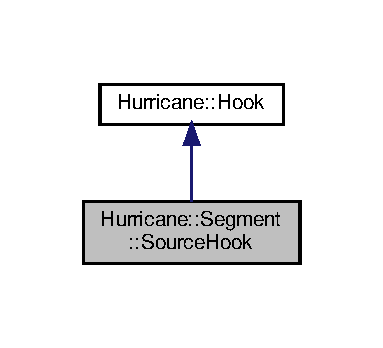
\includegraphics[width=184pt]{classHurricane_1_1Segment_1_1SourceHook__inherit__graph}
\end{center}
\end{figure}
\doxysubsection*{Additional Inherited Members}


\doxysubsection{Detailed Description}
With segments, a new type of \mbox{\hyperlink{classHurricane_1_1Hook}{Hook}} appears \+: the {\bfseries{\mbox{\hyperlink{classHurricane_1_1Segment_1_1SourceHook}{Source\+Hook}}}}, which allows to attach the segment origin upon an other component, on which it is said to be \char`\"{}anchored\char`\"{}. The \mbox{\hyperlink{classHurricane_1_1Segment_1_1SourceHook}{Source\+Hook}} is always a slave hook. 

The documentation for this class was generated from the following file\+:\begin{DoxyCompactItemize}
\item 
Segment.\+h\end{DoxyCompactItemize}

\hypertarget{classHurricane_1_1StandardPrivateProperty}{}\doxysection{Hurricane\+::Standard\+Private\+Property$<$ Value, Json\+State $>$ Class Template Reference}
\label{classHurricane_1_1StandardPrivateProperty}\index{Hurricane::StandardPrivateProperty$<$ Value, JsonState $>$@{Hurricane::StandardPrivateProperty$<$ Value, JsonState $>$}}


\mbox{\hyperlink{classHurricane_1_1StandardPrivateProperty}{Standard\+Private\+Property}} description ({\bfseries{API}})  




Inheritance diagram for Hurricane\+::Standard\+Private\+Property$<$ Value, Json\+State $>$\+:\nopagebreak
\begin{figure}[H]
\begin{center}
\leavevmode
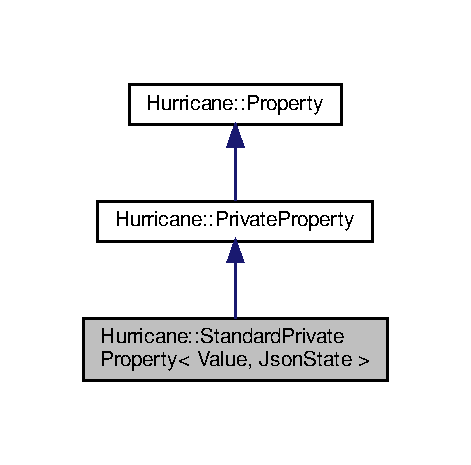
\includegraphics[width=226pt]{classHurricane_1_1StandardPrivateProperty__inherit__graph}
\end{center}
\end{figure}
\doxysubsection*{Additional Inherited Members}


\doxysubsection{Detailed Description}
\subsubsection*{template$<$typename Value, typename Json\+State = Json\+Disabled$>$\newline
class Hurricane\+::\+Standard\+Private\+Property$<$ Value, Json\+State $>$}

\mbox{\hyperlink{classHurricane_1_1StandardPrivateProperty}{Standard\+Private\+Property}} description ({\bfseries{API}}) 

\hypertarget{classHurricane_1_1StandardPrivateProperty_secStandardPrivatePropertyIntro}{}\doxysubsection{Introduction}\label{classHurricane_1_1StandardPrivateProperty_secStandardPrivatePropertyIntro}
Those properties allow to assign to an object a relation between a name and a value. 

The documentation for this class was generated from the following file\+:\begin{DoxyCompactItemize}
\item 
Property.\+h\end{DoxyCompactItemize}

\hypertarget{classHurricane_1_1StandardRelation}{}\doxysection{Hurricane\+::Standard\+Relation Class Reference}
\label{classHurricane_1_1StandardRelation}\index{Hurricane::StandardRelation@{Hurricane::StandardRelation}}


\mbox{\hyperlink{classHurricane_1_1StandardRelation}{Standard\+Relation}} description ({\bfseries{API}})  




Inheritance diagram for Hurricane\+::Standard\+Relation\+:\nopagebreak
\begin{figure}[H]
\begin{center}
\leavevmode
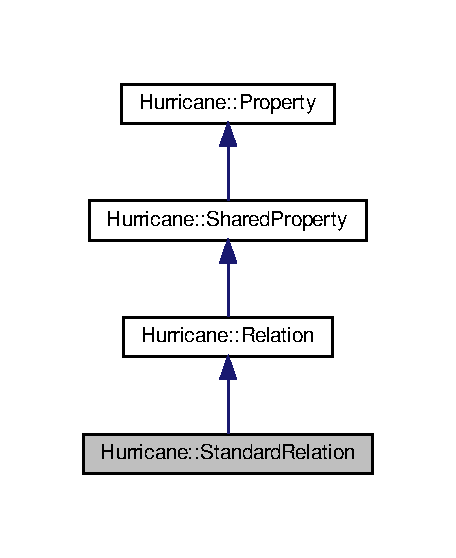
\includegraphics[width=219pt]{classHurricane_1_1StandardRelation__inherit__graph}
\end{center}
\end{figure}
\doxysubsection*{Additional Inherited Members}


\doxysubsection{Detailed Description}
\mbox{\hyperlink{classHurricane_1_1StandardRelation}{Standard\+Relation}} description ({\bfseries{API}}) 

The documentation for this class was generated from the following file\+:\begin{DoxyCompactItemize}
\item 
Relation.\+h\end{DoxyCompactItemize}

\hypertarget{classHurricane_1_1StandardSharedProperty}{}\doxysection{Hurricane\+::Standard\+Shared\+Property$<$ Value $>$ Class Template Reference}
\label{classHurricane_1_1StandardSharedProperty}\index{Hurricane::StandardSharedProperty$<$ Value $>$@{Hurricane::StandardSharedProperty$<$ Value $>$}}


\mbox{\hyperlink{classHurricane_1_1StandardSharedProperty}{Standard\+Shared\+Property}} description ({\bfseries{API}})  




Inheritance diagram for Hurricane\+::Standard\+Shared\+Property$<$ Value $>$\+:\nopagebreak
\begin{figure}[H]
\begin{center}
\leavevmode
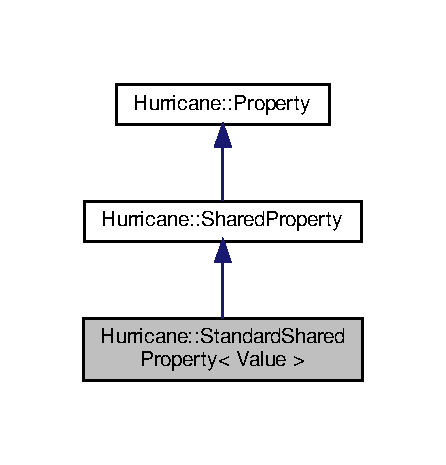
\includegraphics[width=214pt]{classHurricane_1_1StandardSharedProperty__inherit__graph}
\end{center}
\end{figure}
\doxysubsection*{Additional Inherited Members}


\doxysubsection{Detailed Description}
\subsubsection*{template$<$typename Value$>$\newline
class Hurricane\+::\+Standard\+Shared\+Property$<$ Value $>$}

\mbox{\hyperlink{classHurricane_1_1StandardSharedProperty}{Standard\+Shared\+Property}} description ({\bfseries{API}}) 

\hypertarget{classHurricane_1_1StandardSharedProperty_secStandardSharedPropertyIntro}{}\doxysubsection{Introduction}\label{classHurricane_1_1StandardSharedProperty_secStandardSharedPropertyIntro}
Those properties allow to assign to a set of objects a relation between a name and a value. 

The documentation for this class was generated from the following file\+:\begin{DoxyCompactItemize}
\item 
Property.\+h\end{DoxyCompactItemize}

\hypertarget{classHurricane_1_1SubSetCollection}{}\doxysection{Hurricane\+::Sub\+Set\+Collection$<$ Type $>$ Class Template Reference}
\label{classHurricane_1_1SubSetCollection}\index{Hurricane::SubSetCollection$<$ Type $>$@{Hurricane::SubSetCollection$<$ Type $>$}}


Applies a \mbox{\hyperlink{classHurricane_1_1Filter}{Filter}} to a \mbox{\hyperlink{classHurricane_1_1Collection}{Collection}}.  




Inheritance diagram for Hurricane\+::Sub\+Set\+Collection$<$ Type $>$\+:\nopagebreak
\begin{figure}[H]
\begin{center}
\leavevmode
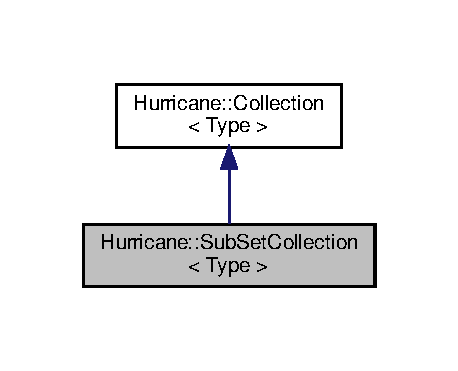
\includegraphics[width=220pt]{classHurricane_1_1SubSetCollection__inherit__graph}
\end{center}
\end{figure}
\doxysubsection*{Public Member Functions}
\begin{Indent}\textbf{ Collection Collection}\par
{\em \hypertarget{Collection_8h_secCollectionUtilitarians}{}\doxysubsection{Utilitarians}\label{Collection_8h_secCollectionUtilitarians}
{\bfseries{Collection\+::\+Fill}} {\bfseries{Collection\+::\+Fill}} {\bfseries{Collection\+::\+Fill}} \begin{DoxyRemark}{Remarks}
The elements are added to the container in the order with which the collection is visited. So the same order will appear in a list or a vector, but for a set they will be inserted according to the set ordering method. 
\end{DoxyRemark}
}\begin{DoxyCompactItemize}
\item 
\mbox{\hyperlink{classHurricane_1_1SubSetCollection_a6da1f511e27351cdc8b56bda7fbc44e8}{Sub\+Set\+Collection}} (const \mbox{\hyperlink{classHurricane_1_1Collection}{Collection}}$<$ Type $>$ \&collection, const \mbox{\hyperlink{classHurricane_1_1Filter}{Filter}}$<$ Type $>$ \&filter)
\item 
\mbox{\hyperlink{classHurricane_1_1SubSetCollection_ad4e0bd9554d898f3991585758dbf2aac}{Sub\+Set\+Collection}} (const \mbox{\hyperlink{classHurricane_1_1SubSetCollection}{Sub\+Set\+Collection}} \&sub\+Set\+Collection)
\end{DoxyCompactItemize}
\end{Indent}


\doxysubsection{Detailed Description}
\subsubsection*{template$<$class Type$>$\newline
class Hurricane\+::\+Sub\+Set\+Collection$<$ Type $>$}

Applies a \mbox{\hyperlink{classHurricane_1_1Filter}{Filter}} to a \mbox{\hyperlink{classHurricane_1_1Collection}{Collection}}. 

Build a sub-\/\+Collection of all the elements of the primary that match the \mbox{\hyperlink{classHurricane_1_1Filter}{Filter}} criterion. 

\doxysubsection{Constructor \& Destructor Documentation}
\mbox{\Hypertarget{classHurricane_1_1SubSetCollection_a6da1f511e27351cdc8b56bda7fbc44e8}\label{classHurricane_1_1SubSetCollection_a6da1f511e27351cdc8b56bda7fbc44e8}} 
\index{Hurricane::SubSetCollection$<$ Type $>$@{Hurricane::SubSetCollection$<$ Type $>$}!SubSetCollection@{SubSetCollection}}
\index{SubSetCollection@{SubSetCollection}!Hurricane::SubSetCollection$<$ Type $>$@{Hurricane::SubSetCollection$<$ Type $>$}}
\doxysubsubsection{\texorpdfstring{SubSetCollection()}{SubSetCollection()}\hspace{0.1cm}{\footnotesize\ttfamily [1/2]}}
{\footnotesize\ttfamily template$<$class Type $>$ \\
\mbox{\hyperlink{classHurricane_1_1SubSetCollection}{Hurricane\+::\+Sub\+Set\+Collection}}$<$ Type $>$\+::\mbox{\hyperlink{classHurricane_1_1SubSetCollection}{Sub\+Set\+Collection}} (\begin{DoxyParamCaption}\item[{const \mbox{\hyperlink{classHurricane_1_1Collection}{Collection}}$<$ Type $>$ \&}]{collection,  }\item[{const \mbox{\hyperlink{classHurricane_1_1Filter}{Filter}}$<$ Type $>$ \&}]{filter }\end{DoxyParamCaption})\hspace{0.3cm}{\ttfamily [inline]}}

Constructor from a primary \mbox{\hyperlink{classHurricane_1_1Collection}{Collection}} and a \mbox{\hyperlink{classHurricane_1_1Filter}{Filter}}. \mbox{\Hypertarget{classHurricane_1_1SubSetCollection_ad4e0bd9554d898f3991585758dbf2aac}\label{classHurricane_1_1SubSetCollection_ad4e0bd9554d898f3991585758dbf2aac}} 
\index{Hurricane::SubSetCollection$<$ Type $>$@{Hurricane::SubSetCollection$<$ Type $>$}!SubSetCollection@{SubSetCollection}}
\index{SubSetCollection@{SubSetCollection}!Hurricane::SubSetCollection$<$ Type $>$@{Hurricane::SubSetCollection$<$ Type $>$}}
\doxysubsubsection{\texorpdfstring{SubSetCollection()}{SubSetCollection()}\hspace{0.1cm}{\footnotesize\ttfamily [2/2]}}
{\footnotesize\ttfamily template$<$class Type $>$ \\
\mbox{\hyperlink{classHurricane_1_1SubSetCollection}{Hurricane\+::\+Sub\+Set\+Collection}}$<$ Type $>$\+::\mbox{\hyperlink{classHurricane_1_1SubSetCollection}{Sub\+Set\+Collection}} (\begin{DoxyParamCaption}\item[{const \mbox{\hyperlink{classHurricane_1_1SubSetCollection}{Sub\+Set\+Collection}}$<$ Type $>$ \&}]{sub\+Set\+Collection }\end{DoxyParamCaption})\hspace{0.3cm}{\ttfamily [inline]}}

Copy constructor. 

The documentation for this class was generated from the following files\+:\begin{DoxyCompactItemize}
\item 
Collection.\+h\item 
Collection.\+dox\end{DoxyCompactItemize}

\hypertarget{classHurricane_1_1SubTypeCollection}{}\doxysection{Hurricane\+::Sub\+Type\+Collection$<$ Type, Sub\+Type $>$ Class Template Reference}
\label{classHurricane_1_1SubTypeCollection}\index{Hurricane::SubTypeCollection$<$ Type, SubType $>$@{Hurricane::SubTypeCollection$<$ Type, SubType $>$}}


Applies a Type \mbox{\hyperlink{classHurricane_1_1Filter}{Filter}} to a \mbox{\hyperlink{classHurricane_1_1Collection}{Collection}}.  




Inheritance diagram for Hurricane\+::Sub\+Type\+Collection$<$ Type, Sub\+Type $>$\+:\nopagebreak
\begin{figure}[H]
\begin{center}
\leavevmode
\includegraphics[width=226pt]{classHurricane_1_1SubTypeCollection__inherit__graph}
\end{center}
\end{figure}
\doxysubsection*{Public Member Functions}
\begin{Indent}\textbf{ Collection Collection}\par
{\em \hypertarget{Collection_8h_secCollectionUtilitarians}{}\doxysubsection{Utilitarians}\label{Collection_8h_secCollectionUtilitarians}
{\bfseries{Collection\+::\+Fill}} {\bfseries{Collection\+::\+Fill}} {\bfseries{Collection\+::\+Fill}} \begin{DoxyRemark}{Remarks}
The elements are added to the container in the order with which the collection is visited. So the same order will appear in a list or a vector, but for a set they will be inserted according to the set ordering method. 
\end{DoxyRemark}
}\begin{DoxyCompactItemize}
\item 
\mbox{\hyperlink{classHurricane_1_1SubTypeCollection_a0fd6c8e781097e607b813306fd2ad677}{Sub\+Type\+Collection}} (const \mbox{\hyperlink{classHurricane_1_1Collection}{Collection}}$<$ Type $>$ $\ast$collection)
\item 
\mbox{\hyperlink{classHurricane_1_1SubTypeCollection_a09df045ff335493ac3068a865b793291}{Sub\+Type\+Collection}} (const \mbox{\hyperlink{classHurricane_1_1GenericCollection}{Generic\+Collection}}$<$ Type $>$ \&collection)
\item 
\mbox{\hyperlink{classHurricane_1_1SubTypeCollection_a5c223a20f42ebb72d8d4be5ee99bb2d8}{Sub\+Type\+Collection}} (const \mbox{\hyperlink{classHurricane_1_1SubTypeCollection}{Sub\+Type\+Collection}} \&sub\+Type\+Collection)
\end{DoxyCompactItemize}
\end{Indent}


\doxysubsection{Detailed Description}
\subsubsection*{template$<$class Type, class Sub\+Type$>$\newline
class Hurricane\+::\+Sub\+Type\+Collection$<$ Type, Sub\+Type $>$}

Applies a Type \mbox{\hyperlink{classHurricane_1_1Filter}{Filter}} to a \mbox{\hyperlink{classHurricane_1_1Collection}{Collection}}. 

Build a sub-\/\+Collection of all the elements of the primary that are of a certain sub-\/type. The filtering mechanism relies on a {\ttfamily dynamic\+\_\+cast$<$$>$} so there must be an inheritance path between the \mbox{\hyperlink{classHurricane_1_1Collection}{Collection}} type and the sub-\/type. 

\doxysubsection{Constructor \& Destructor Documentation}
\mbox{\Hypertarget{classHurricane_1_1SubTypeCollection_a0fd6c8e781097e607b813306fd2ad677}\label{classHurricane_1_1SubTypeCollection_a0fd6c8e781097e607b813306fd2ad677}} 
\index{Hurricane::SubTypeCollection$<$ Type, SubType $>$@{Hurricane::SubTypeCollection$<$ Type, SubType $>$}!SubTypeCollection@{SubTypeCollection}}
\index{SubTypeCollection@{SubTypeCollection}!Hurricane::SubTypeCollection$<$ Type, SubType $>$@{Hurricane::SubTypeCollection$<$ Type, SubType $>$}}
\doxysubsubsection{\texorpdfstring{SubTypeCollection()}{SubTypeCollection()}\hspace{0.1cm}{\footnotesize\ttfamily [1/3]}}
{\footnotesize\ttfamily template$<$class Type , class Sub\+Type $>$ \\
\mbox{\hyperlink{classHurricane_1_1SubTypeCollection}{Hurricane\+::\+Sub\+Type\+Collection}}$<$ Type, Sub\+Type $>$\+::\mbox{\hyperlink{classHurricane_1_1SubTypeCollection}{Sub\+Type\+Collection}} (\begin{DoxyParamCaption}\item[{const \mbox{\hyperlink{classHurricane_1_1Collection}{Collection}}$<$ Type $>$ $\ast$}]{collection }\end{DoxyParamCaption})\hspace{0.3cm}{\ttfamily [inline]}}

Constructor from a primary \mbox{\hyperlink{classHurricane_1_1Collection}{Collection}} and a \mbox{\hyperlink{classHurricane_1_1Filter}{Filter}}. \mbox{\Hypertarget{classHurricane_1_1SubTypeCollection_a09df045ff335493ac3068a865b793291}\label{classHurricane_1_1SubTypeCollection_a09df045ff335493ac3068a865b793291}} 
\index{Hurricane::SubTypeCollection$<$ Type, SubType $>$@{Hurricane::SubTypeCollection$<$ Type, SubType $>$}!SubTypeCollection@{SubTypeCollection}}
\index{SubTypeCollection@{SubTypeCollection}!Hurricane::SubTypeCollection$<$ Type, SubType $>$@{Hurricane::SubTypeCollection$<$ Type, SubType $>$}}
\doxysubsubsection{\texorpdfstring{SubTypeCollection()}{SubTypeCollection()}\hspace{0.1cm}{\footnotesize\ttfamily [2/3]}}
{\footnotesize\ttfamily template$<$class Type , class Sub\+Type $>$ \\
\mbox{\hyperlink{classHurricane_1_1SubTypeCollection}{Hurricane\+::\+Sub\+Type\+Collection}}$<$ Type, Sub\+Type $>$\+::\mbox{\hyperlink{classHurricane_1_1SubTypeCollection}{Sub\+Type\+Collection}} (\begin{DoxyParamCaption}\item[{const \mbox{\hyperlink{classHurricane_1_1GenericCollection}{Generic\+Collection}}$<$ Type $>$ \&}]{collection }\end{DoxyParamCaption})\hspace{0.3cm}{\ttfamily [inline]}}

Constructor from a primary \mbox{\hyperlink{classHurricane_1_1Collection}{Collection}} and a \mbox{\hyperlink{classHurricane_1_1Filter}{Filter}}. \mbox{\Hypertarget{classHurricane_1_1SubTypeCollection_a5c223a20f42ebb72d8d4be5ee99bb2d8}\label{classHurricane_1_1SubTypeCollection_a5c223a20f42ebb72d8d4be5ee99bb2d8}} 
\index{Hurricane::SubTypeCollection$<$ Type, SubType $>$@{Hurricane::SubTypeCollection$<$ Type, SubType $>$}!SubTypeCollection@{SubTypeCollection}}
\index{SubTypeCollection@{SubTypeCollection}!Hurricane::SubTypeCollection$<$ Type, SubType $>$@{Hurricane::SubTypeCollection$<$ Type, SubType $>$}}
\doxysubsubsection{\texorpdfstring{SubTypeCollection()}{SubTypeCollection()}\hspace{0.1cm}{\footnotesize\ttfamily [3/3]}}
{\footnotesize\ttfamily template$<$class Type , class Sub\+Type $>$ \\
\mbox{\hyperlink{classHurricane_1_1SubTypeCollection}{Hurricane\+::\+Sub\+Type\+Collection}}$<$ Type, Sub\+Type $>$\+::\mbox{\hyperlink{classHurricane_1_1SubTypeCollection}{Sub\+Type\+Collection}} (\begin{DoxyParamCaption}\item[{const \mbox{\hyperlink{classHurricane_1_1SubTypeCollection}{Sub\+Type\+Collection}}$<$ Type, Sub\+Type $>$ \&}]{sub\+Type\+Collection }\end{DoxyParamCaption})\hspace{0.3cm}{\ttfamily [inline]}}

Copy Constructor. 

The documentation for this class was generated from the following files\+:\begin{DoxyCompactItemize}
\item 
Collection.\+h\item 
Collection.\+dox\end{DoxyCompactItemize}

\hypertarget{classHurricane_1_1Tabulation}{}\doxysection{Hurricane\+::Tabulation Class Reference}
\label{classHurricane_1_1Tabulation}\index{Hurricane::Tabulation@{Hurricane::Tabulation}}


\mbox{\hyperlink{classHurricane_1_1Tabulation}{Tabulation}} description ({\bfseries{API}})  


\doxysubsection*{Public Member Functions}
\begin{DoxyCompactItemize}
\item 
\mbox{\hyperlink{classHurricane_1_1Tabulation_a59932db80223de3ba630592218cb1005}{Tabulation}} (const string \&s=\char`\"{}   \char`\"{})
\item 
\mbox{\hyperlink{classHurricane_1_1Tabulation_a78f765f6b4fc0e629f5d3babf7a785aa}{Tabulation}} (const \mbox{\hyperlink{classHurricane_1_1Tabulation}{Tabulation}} \&tabulation)
\item 
\mbox{\hyperlink{classHurricane_1_1Tabulation_aa549d938b7534f8eae8e8e954b1f3207}{$\sim$\+Tabulation}} ()
\item 
\mbox{\hyperlink{classHurricane_1_1Tabulation}{Tabulation}} \& \mbox{\hyperlink{classHurricane_1_1Tabulation_a33c4a5152580309407e3e2730f07c321}{operator=}} (const \mbox{\hyperlink{classHurricane_1_1Tabulation}{Tabulation}} \&tabulation)
\item 
\mbox{\hyperlink{classHurricane_1_1Tabulation}{Tabulation}} \& \mbox{\hyperlink{classHurricane_1_1Tabulation_ad108353099b0755a45a18ec1ab6c0b7c}{operator++}} ()
\item 
\mbox{\hyperlink{classHurricane_1_1Tabulation}{Tabulation}} \mbox{\hyperlink{classHurricane_1_1Tabulation_ae609e34474086ac1b9748368d798acae}{operator++}} (int)
\item 
\mbox{\hyperlink{classHurricane_1_1Tabulation}{Tabulation}} \& \mbox{\hyperlink{classHurricane_1_1Tabulation_af95446070605eb5d2ce89e9b8b3049be}{operator-\/-\/}} ()
\item 
\mbox{\hyperlink{classHurricane_1_1Tabulation}{Tabulation}} \mbox{\hyperlink{classHurricane_1_1Tabulation_a9bdb9f81cd412ffcfb1da048b75cbd99}{operator-\/-\/}} (int)
\end{DoxyCompactItemize}


\doxysubsection{Detailed Description}
\mbox{\hyperlink{classHurricane_1_1Tabulation}{Tabulation}} description ({\bfseries{API}}) 

\hypertarget{classHurricane_1_1Tabulation_secTabulationIntro}{}\doxysubsection{Introduction}\label{classHurricane_1_1Tabulation_secTabulationIntro}
This object provides an indentation capability for printing readable texts.\hypertarget{classHurricane_1_1Tabulation_secTabulationNewGlobalVariable}{}\doxysubsection{New global variable}\label{classHurricane_1_1Tabulation_secTabulationNewGlobalVariable}

\begin{DoxyCode}{0}
\DoxyCodeLine{\mbox{\hyperlink{classHurricane_1_1Tabulation_a59932db80223de3ba630592218cb1005}{Tabulation}} tab(\textcolor{stringliteral}{"{}    "{}});}

\end{DoxyCode}
 Represents the global tabulation variable usable by all application programmers. The elementary tabulation being fixed to 3 space characters.\hypertarget{classHurricane_1_1Tabulation_secTabulationUsage}{}\doxysubsection{Usage}\label{classHurricane_1_1Tabulation_secTabulationUsage}
Let us write a sample code of printing a succinct cell description \+: 
\begin{DoxyCode}{0}
\DoxyCodeLine{\textcolor{keywordtype}{void} Describe(Cell* cell)}
\DoxyCodeLine{\textcolor{comment}{// **********************}}
\DoxyCodeLine{\{}
\DoxyCodeLine{   cout << tab++ << \textcolor{stringliteral}{"{}cell : "{}} << cellGetName() << endl;}
\DoxyCodeLine{   \textcolor{keywordflow}{if} (!cellGetInstances().IsEmpty()) \{}
\DoxyCodeLine{      cout << tab++ << \textcolor{stringliteral}{"{}instances : \{"{}} << endl;}
\DoxyCodeLine{      for\_each\_instance(instance, cellGetInstances()) \{}
\DoxyCodeLine{         cout << tab << \textcolor{stringliteral}{"{}instance : "{}} << instanceGetName() << endl;}
\DoxyCodeLine{         end\_for;}
\DoxyCodeLine{      \}}
\DoxyCodeLine{      cout << -\/-\/tab << \textcolor{stringliteral}{"{}\}"{}};}
\DoxyCodeLine{   \}}
\DoxyCodeLine{   \textcolor{keywordflow}{if} (!cellGetNets().IsEmpty()) \{}
\DoxyCodeLine{      cout << tab++ << \textcolor{stringliteral}{"{}nets : \{"{}} << endl;}
\DoxyCodeLine{      for\_each\_net(net, cellGetNets()) \{}
\DoxyCodeLine{         cout << tab++ << \textcolor{stringliteral}{"{}net : "{}} << netGetName() << endl;}
\DoxyCodeLine{         \textcolor{keywordflow}{if} (!netGetPlugs().IsEmpty()) \{}
\DoxyCodeLine{            cout << tab++ << \textcolor{stringliteral}{"{}plugs : \{"{}} << endl;}
\DoxyCodeLine{            for\_each\_plug(plug, netGetPlugs()) \{}
\DoxyCodeLine{               cout << tab << \textcolor{stringliteral}{"{}master\_net : "{}}}
\DoxyCodeLine{                    << plugGetMasterNet()GetName() << endl;}
\DoxyCodeLine{               end\_for;}
\DoxyCodeLine{            \}}
\DoxyCodeLine{            cout << -\/-\/tab << "{}\}"{};}
\DoxyCodeLine{         \}}
\DoxyCodeLine{         end\_for;}
\DoxyCodeLine{      \}}
\DoxyCodeLine{      cout << -\/-\/tab << "{}\}"{};}
\DoxyCodeLine{   \}}
\DoxyCodeLine{   -\/-\/tab;}
\DoxyCodeLine{\}}

\end{DoxyCode}
 The call \+: 
\begin{DoxyCode}{0}
\DoxyCodeLine{Describe(cell);}

\end{DoxyCode}
 Will print the result in the following form \+: 
\begin{DoxyCode}{0}
\DoxyCodeLine{cell : ...}
\DoxyCodeLine{   instances : \{}
\DoxyCodeLine{      instance : ...}
\DoxyCodeLine{      instance : ...}
\DoxyCodeLine{      ...}
\DoxyCodeLine{   \}}
\DoxyCodeLine{   nets : \{}
\DoxyCodeLine{      net : ...}
\DoxyCodeLine{         plugs : \{}
\DoxyCodeLine{            master\_net : ...}
\DoxyCodeLine{            master\_net : ...}
\DoxyCodeLine{            ...}
\DoxyCodeLine{         \}}
\DoxyCodeLine{      net : ...}
\DoxyCodeLine{         plugs : \{}
\DoxyCodeLine{            master\_net : ...}
\DoxyCodeLine{            master\_net : ...}
\DoxyCodeLine{            ...}
\DoxyCodeLine{         \}}
\DoxyCodeLine{      ...}
\DoxyCodeLine{   \}}

\end{DoxyCode}
\hypertarget{classHurricane_1_1Tabulation_secTabulationRemark}{}\doxysubsection{Remark}\label{classHurricane_1_1Tabulation_secTabulationRemark}
Of course this automatic indentation works also in recursive mode. Its main interest is for that purpose because you don\textquotesingle{}t need to transfer through recursive function calls an additional argument for controling the indentation when formating print-\/outs. 

\doxysubsection{Constructor \& Destructor Documentation}
\mbox{\Hypertarget{classHurricane_1_1Tabulation_a59932db80223de3ba630592218cb1005}\label{classHurricane_1_1Tabulation_a59932db80223de3ba630592218cb1005}} 
\index{Hurricane::Tabulation@{Hurricane::Tabulation}!Tabulation@{Tabulation}}
\index{Tabulation@{Tabulation}!Hurricane::Tabulation@{Hurricane::Tabulation}}
\doxysubsubsection{\texorpdfstring{Tabulation()}{Tabulation()}\hspace{0.1cm}{\footnotesize\ttfamily [1/2]}}
{\footnotesize\ttfamily Hurricane\+::\+Tabulation\+::\+Tabulation (\begin{DoxyParamCaption}\item[{const string \&}]{s = {\ttfamily \char`\"{}~~~\char`\"{}} }\end{DoxyParamCaption})}

Default constructor \+: The string {\ttfamily $<$s$>$} represents the elementary tabulation (fixed by default to 3 space characters) \mbox{\Hypertarget{classHurricane_1_1Tabulation_a78f765f6b4fc0e629f5d3babf7a785aa}\label{classHurricane_1_1Tabulation_a78f765f6b4fc0e629f5d3babf7a785aa}} 
\index{Hurricane::Tabulation@{Hurricane::Tabulation}!Tabulation@{Tabulation}}
\index{Tabulation@{Tabulation}!Hurricane::Tabulation@{Hurricane::Tabulation}}
\doxysubsubsection{\texorpdfstring{Tabulation()}{Tabulation()}\hspace{0.1cm}{\footnotesize\ttfamily [2/2]}}
{\footnotesize\ttfamily Hurricane\+::\+Tabulation\+::\+Tabulation (\begin{DoxyParamCaption}\item[{const \mbox{\hyperlink{classHurricane_1_1Tabulation}{Tabulation}} \&}]{tabulation }\end{DoxyParamCaption})}

Copy constructor. \mbox{\Hypertarget{classHurricane_1_1Tabulation_aa549d938b7534f8eae8e8e954b1f3207}\label{classHurricane_1_1Tabulation_aa549d938b7534f8eae8e8e954b1f3207}} 
\index{Hurricane::Tabulation@{Hurricane::Tabulation}!````~Tabulation@{$\sim$Tabulation}}
\index{````~Tabulation@{$\sim$Tabulation}!Hurricane::Tabulation@{Hurricane::Tabulation}}
\doxysubsubsection{\texorpdfstring{$\sim$Tabulation()}{~Tabulation()}}
{\footnotesize\ttfamily Hurricane\+::\+Tabulation\+::$\sim$\+Tabulation (\begin{DoxyParamCaption}{ }\end{DoxyParamCaption})}

No description. 

\doxysubsection{Member Function Documentation}
\mbox{\Hypertarget{classHurricane_1_1Tabulation_a33c4a5152580309407e3e2730f07c321}\label{classHurricane_1_1Tabulation_a33c4a5152580309407e3e2730f07c321}} 
\index{Hurricane::Tabulation@{Hurricane::Tabulation}!operator=@{operator=}}
\index{operator=@{operator=}!Hurricane::Tabulation@{Hurricane::Tabulation}}
\doxysubsubsection{\texorpdfstring{operator=()}{operator=()}}
{\footnotesize\ttfamily \mbox{\hyperlink{classHurricane_1_1Tabulation}{Tabulation}} \& Hurricane\+::\+Tabulation\+::operator= (\begin{DoxyParamCaption}\item[{const \mbox{\hyperlink{classHurricane_1_1Tabulation}{Tabulation}} \&}]{tabulation }\end{DoxyParamCaption})}

Assignment operator. \mbox{\Hypertarget{classHurricane_1_1Tabulation_ad108353099b0755a45a18ec1ab6c0b7c}\label{classHurricane_1_1Tabulation_ad108353099b0755a45a18ec1ab6c0b7c}} 
\index{Hurricane::Tabulation@{Hurricane::Tabulation}!operator++@{operator++}}
\index{operator++@{operator++}!Hurricane::Tabulation@{Hurricane::Tabulation}}
\doxysubsubsection{\texorpdfstring{operator++()}{operator++()}\hspace{0.1cm}{\footnotesize\ttfamily [1/2]}}
{\footnotesize\ttfamily \mbox{\hyperlink{classHurricane_1_1Tabulation}{Tabulation}} \& Hurricane\+::\+Tabulation\+::operator++ (\begin{DoxyParamCaption}{ }\end{DoxyParamCaption})}

Incrementation operator \+: returns the tabulation augmented of an elementary tabulation. \mbox{\Hypertarget{classHurricane_1_1Tabulation_ae609e34474086ac1b9748368d798acae}\label{classHurricane_1_1Tabulation_ae609e34474086ac1b9748368d798acae}} 
\index{Hurricane::Tabulation@{Hurricane::Tabulation}!operator++@{operator++}}
\index{operator++@{operator++}!Hurricane::Tabulation@{Hurricane::Tabulation}}
\doxysubsubsection{\texorpdfstring{operator++()}{operator++()}\hspace{0.1cm}{\footnotesize\ttfamily [2/2]}}
{\footnotesize\ttfamily \mbox{\hyperlink{classHurricane_1_1Tabulation}{Tabulation}} Hurricane\+::\+Tabulation\+::operator++ (\begin{DoxyParamCaption}\item[{int}]{ }\end{DoxyParamCaption})}

Postfixed version of the incrementation operator \+: the tabulation is augmented of an elementary tabulation, but returns the previous tabulation. \mbox{\Hypertarget{classHurricane_1_1Tabulation_af95446070605eb5d2ce89e9b8b3049be}\label{classHurricane_1_1Tabulation_af95446070605eb5d2ce89e9b8b3049be}} 
\index{Hurricane::Tabulation@{Hurricane::Tabulation}!operator-\/-\/@{operator-\/-\/}}
\index{operator-\/-\/@{operator-\/-\/}!Hurricane::Tabulation@{Hurricane::Tabulation}}
\doxysubsubsection{\texorpdfstring{operator-\/-\/()}{operator--()}\hspace{0.1cm}{\footnotesize\ttfamily [1/2]}}
{\footnotesize\ttfamily \mbox{\hyperlink{classHurricane_1_1Tabulation}{Tabulation}} \& Hurricane\+::\+Tabulation\+::operator-\/-\/ (\begin{DoxyParamCaption}{ }\end{DoxyParamCaption})}

Decrementation operator \+: returns the tabulation reduced of an elementary tabulation. \mbox{\Hypertarget{classHurricane_1_1Tabulation_a9bdb9f81cd412ffcfb1da048b75cbd99}\label{classHurricane_1_1Tabulation_a9bdb9f81cd412ffcfb1da048b75cbd99}} 
\index{Hurricane::Tabulation@{Hurricane::Tabulation}!operator-\/-\/@{operator-\/-\/}}
\index{operator-\/-\/@{operator-\/-\/}!Hurricane::Tabulation@{Hurricane::Tabulation}}
\doxysubsubsection{\texorpdfstring{operator-\/-\/()}{operator--()}\hspace{0.1cm}{\footnotesize\ttfamily [2/2]}}
{\footnotesize\ttfamily \mbox{\hyperlink{classHurricane_1_1Tabulation}{Tabulation}} Hurricane\+::\+Tabulation\+::operator-\/-\/ (\begin{DoxyParamCaption}\item[{int}]{ }\end{DoxyParamCaption})}

Postfixed version of the decrementation operator \+: the tabulation is reduced of an elementary tabulation, but returns the previous tabulation. 

The documentation for this class was generated from the following files\+:\begin{DoxyCompactItemize}
\item 
Tabulation.\+h\item 
Tabulation.\+dox\end{DoxyCompactItemize}

\hypertarget{classHurricane_1_1Segment_1_1TargetHook}{}\doxysection{Hurricane\+::Segment\+::Target\+Hook Class Reference}
\label{classHurricane_1_1Segment_1_1TargetHook}\index{Hurricane::Segment::TargetHook@{Hurricane::Segment::TargetHook}}


Inheritance diagram for Hurricane\+::Segment\+::Target\+Hook\+:\nopagebreak
\begin{figure}[H]
\begin{center}
\leavevmode
\includegraphics[width=184pt]{classHurricane_1_1Segment_1_1TargetHook__inherit__graph}
\end{center}
\end{figure}
\doxysubsection*{Additional Inherited Members}


\doxysubsection{Detailed Description}
With segments, a new type of \mbox{\hyperlink{classHurricane_1_1Hook}{Hook}} appears \+: the {\bfseries{\mbox{\hyperlink{classHurricane_1_1Segment_1_1TargetHook}{Target\+Hook}}}}, which allows to attach the segment extremity upon an other component, on which it is said to be \char`\"{}anchored\char`\"{}. The \mbox{\hyperlink{classHurricane_1_1Segment_1_1TargetHook}{Target\+Hook}} is always a slave hook. 

The documentation for this class was generated from the following file\+:\begin{DoxyCompactItemize}
\item 
Segment.\+h\end{DoxyCompactItemize}

\hypertarget{classHurricane_1_1Technology}{}\doxysection{Hurricane\+::Technology Class Reference}
\label{classHurricane_1_1Technology}\index{Hurricane::Technology@{Hurricane::Technology}}


Technological rules description ({\bfseries{API}}).  




Inheritance diagram for Hurricane\+::Technology\+:\nopagebreak
\begin{figure}[H]
\begin{center}
\leavevmode
\includegraphics[width=194pt]{classHurricane_1_1Technology__inherit__graph}
\end{center}
\end{figure}
\doxysubsection*{Public Member Functions}
\begin{DoxyCompactItemize}
\item 
bool \mbox{\hyperlink{classHurricane_1_1Technology_ae5590e455d35f76531a6feb0c0f111a2}{is\+Metal}} (const \mbox{\hyperlink{classHurricane_1_1Layer}{Layer}} $\ast$) const
\item 
\mbox{\hyperlink{classHurricane_1_1DataBase}{Data\+Base}} $\ast$ \mbox{\hyperlink{classHurricane_1_1Technology_acf836e738fba14fa493b0e08148cc3ee}{get\+Data\+Base}} () const
\item 
const \mbox{\hyperlink{classHurricane_1_1Name}{Name}} \& \mbox{\hyperlink{classHurricane_1_1Technology_ae466071aa1991c853ee71af12fa62d4e}{get\+Name}} () const
\item 
\mbox{\hyperlink{classHurricane_1_1Layer}{Layer}} $\ast$ \mbox{\hyperlink{classHurricane_1_1Technology_a4ec69c9f8f6b483885f1900c56a97b61}{get\+Layer}} (const \mbox{\hyperlink{classHurricane_1_1Name}{Name}} \&) const
\item 
\mbox{\hyperlink{classHurricane_1_1BasicLayer}{Basic\+Layer}} $\ast$ \mbox{\hyperlink{classHurricane_1_1Technology_ab096154ce9485cef02244f0037efd4fb}{get\+Basic\+Layer}} (const \mbox{\hyperlink{classHurricane_1_1Name}{Name}} \&) const
\item 
\mbox{\hyperlink{classHurricane_1_1RegularLayer}{Regular\+Layer}} $\ast$ \mbox{\hyperlink{classHurricane_1_1Technology_a0e93f2f749ee9b6efd30de4ef74546cc}{get\+Regular\+Layer}} (const \mbox{\hyperlink{classHurricane_1_1Name}{Name}} \&) const
\item 
\mbox{\hyperlink{classHurricane_1_1ViaLayer}{Via\+Layer}} $\ast$ \mbox{\hyperlink{classHurricane_1_1Technology_a9edd085c08487642dd8745b66cf40c76}{get\+Via\+Layer}} (const \mbox{\hyperlink{classHurricane_1_1Name}{Name}} \&) const
\item 
\mbox{\hyperlink{namespaceHurricane_a7b7200a36ab7ce8a157ddbe78b625f38}{Layers}} \mbox{\hyperlink{classHurricane_1_1Technology_a4e58c5ae8e3e82d7fe1b3bb939d6a633}{get\+Layers}} () const
\item 
Basic\+Layers \mbox{\hyperlink{classHurricane_1_1Technology_a7fccff9da6604fafb90408ba56184fc0}{get\+Basic\+Layers}} () const
\item 
Basic\+Layers \mbox{\hyperlink{classHurricane_1_1Technology_a997457824046ea63eba51210a8e23f85}{get\+Basic\+Layers}} (const \mbox{\hyperlink{classHurricane_1_1Layer_af5277c670637bd5d910237e7afe01a91}{Layer\+::\+Mask}} \&) const
\item 
Regular\+Layers \mbox{\hyperlink{classHurricane_1_1Technology_abffce542bc1cee054b4a09c64449f3b8}{get\+Regular\+Layers}} () const
\item 
Via\+Layers \mbox{\hyperlink{classHurricane_1_1Technology_aacde973f6a02a232a01f3f618576e1ee}{get\+Via\+Layers}} () const
\item 
\mbox{\hyperlink{classHurricane_1_1Layer}{Layer}} $\ast$ \mbox{\hyperlink{classHurricane_1_1Technology_a2ab8d2c386bf3daeb2b93d92ecbac6b4}{get\+Layer}} (const \mbox{\hyperlink{classHurricane_1_1Layer_af5277c670637bd5d910237e7afe01a91}{Layer\+::\+Mask}} \&, bool use\+Symbolic=true) const
\item 
\mbox{\hyperlink{classHurricane_1_1Layer}{Layer}} $\ast$ \mbox{\hyperlink{classHurricane_1_1Technology_af5723b08c9d289ffef8159ac2ea71b74}{get\+Metal\+Above}} (const \mbox{\hyperlink{classHurricane_1_1Layer}{Layer}} $\ast$, bool use\+Symbolic=true) const
\item 
\mbox{\hyperlink{classHurricane_1_1Layer}{Layer}} $\ast$ \mbox{\hyperlink{classHurricane_1_1Technology_ae02123406c7362cc14413727e8689d5a}{get\+Metal\+Below}} (const \mbox{\hyperlink{classHurricane_1_1Layer}{Layer}} $\ast$, bool use\+Symbolic=true) const
\item 
\mbox{\hyperlink{classHurricane_1_1Layer}{Layer}} $\ast$ \mbox{\hyperlink{classHurricane_1_1Technology_ac7125a8eea871918e74bb295c56caceb}{get\+Cut\+Above}} (const \mbox{\hyperlink{classHurricane_1_1Layer}{Layer}} $\ast$, bool use\+Symbolic=true) const
\item 
\mbox{\hyperlink{classHurricane_1_1Layer}{Layer}} $\ast$ \mbox{\hyperlink{classHurricane_1_1Technology_a3ca39dccc7e19b404181f55777e1b933}{get\+Cut\+Below}} (const \mbox{\hyperlink{classHurricane_1_1Layer}{Layer}} $\ast$, bool use\+Symbolic=true) const
\item 
\mbox{\hyperlink{classHurricane_1_1Layer}{Layer}} $\ast$ \mbox{\hyperlink{classHurricane_1_1Technology_a8209708bc594a307ea39f15a39bbf196}{get\+Via\+Between}} (const \mbox{\hyperlink{classHurricane_1_1Layer}{Layer}} $\ast$, const \mbox{\hyperlink{classHurricane_1_1Layer}{Layer}} $\ast$, bool use\+Symbolic=true) const
\item 
\mbox{\hyperlink{classHurricane_1_1Layer}{Layer}} $\ast$ \mbox{\hyperlink{classHurricane_1_1Technology_a81a3f3e479aeb686c61a2d0fa2931f3b}{get\+Nth\+Metal}} (int) const
\item 
\mbox{\hyperlink{classHurricane_1_1PhysicalRule}{Physical\+Rule}} $\ast$ \mbox{\hyperlink{classHurricane_1_1Technology_a6ab76e8a246a10a395d68341bca9ea96}{get\+Unit\+Rule}} (std\+::string rule\+Name) const
\item 
\mbox{\hyperlink{classHurricane_1_1PhysicalRule}{Physical\+Rule}} $\ast$ \mbox{\hyperlink{classHurricane_1_1Technology_a21ef6f7507785a587e56aecc52a0c0ee}{get\+Physical\+Rule}} (std\+::string rule\+Name, std\+::string layer\+Name) const
\item 
\mbox{\hyperlink{classHurricane_1_1PhysicalRule}{Physical\+Rule}} $\ast$ \mbox{\hyperlink{classHurricane_1_1Technology_aec2ce8a8195e90537e6d35cb3ba8b58f}{get\+Physical\+Rule}} (std\+::string rule\+Name, std\+::string layer1\+Name, std\+::string layer2\+Name) const
\item 
void \mbox{\hyperlink{classHurricane_1_1Technology_a247b75d5cbb85198cea9e5e609304cd0}{set\+Name}} (const \mbox{\hyperlink{classHurricane_1_1Name}{Name}} \&)
\item 
bool \mbox{\hyperlink{classHurricane_1_1Technology_a26c12c5828acaeb33068a2899df1134b}{set\+Symbolic\+Layer}} (const \mbox{\hyperlink{classHurricane_1_1Layer}{Layer}} $\ast$)
\item 
\mbox{\hyperlink{classHurricane_1_1PhysicalRule}{Physical\+Rule}} $\ast$ \mbox{\hyperlink{classHurricane_1_1Technology_a96d62a8b3eb12560a9cb778328f8a301}{add\+Unit\+Rule}} (std\+::string rule\+Name, std\+::string reference)
\item 
\mbox{\hyperlink{classHurricane_1_1PhysicalRule}{Physical\+Rule}} $\ast$ \mbox{\hyperlink{classHurricane_1_1Technology_a267e44b205b97ff46297d16ed278a5bc}{add\+Physical\+Rule}} (std\+::string rule\+Name, std\+::string reference)
\item 
\mbox{\hyperlink{classHurricane_1_1PhysicalRule}{Physical\+Rule}} $\ast$ \mbox{\hyperlink{classHurricane_1_1Technology_a4210936e097a774035bf52bce7d962bc}{add\+Physical\+Rule}} (std\+::string rule\+Name, std\+::string layer\+Name, std\+::string reference)
\item 
\mbox{\hyperlink{classHurricane_1_1PhysicalRule}{Physical\+Rule}} $\ast$ \mbox{\hyperlink{classHurricane_1_1Technology_a3f04a0d9fe9c76fc3c0911c76c120e00}{add\+Physical\+Rule}} (std\+::string rule\+Name, std\+::string layer1\+Name, std\+::string layer2\+Name, std\+::string reference)
\end{DoxyCompactItemize}
\doxysubsection*{Static Public Member Functions}
\begin{DoxyCompactItemize}
\item 
static \mbox{\hyperlink{classHurricane_1_1Technology}{Technology}} $\ast$ \mbox{\hyperlink{classHurricane_1_1Technology_a64670f0d48e9460342005df52f25c152}{create}} (\mbox{\hyperlink{classHurricane_1_1DataBase}{Data\+Base}} $\ast$, const \mbox{\hyperlink{classHurricane_1_1Name}{Name}} \&)
\end{DoxyCompactItemize}


\doxysubsection{Detailed Description}
Technological rules description ({\bfseries{API}}). 

\hypertarget{classHurricane_1_1Technology_sTechnologyIntro}{}\doxysubsection{Introduction}\label{classHurricane_1_1Technology_sTechnologyIntro}
The \mbox{\hyperlink{classHurricane_1_1Technology}{Technology}} object provides the description of all the technology rules needed by the tools, currently it contains\+:


\begin{DoxyItemize}
\item The layers, roughly from bottom (i.\+e. closest to the subtsrate) to top. Layers can be basic, that is, match a real physical layer, or composite, like for VIAs in symbolic for macro-\/generation. It also provides a connexity table between layers.
\item Three sets of rules describing the technology rules (formerly the {\ttfamily DTR} in Alliance).
\begin{DoxyEnumerate}
\item {\ttfamily Zero \mbox{\hyperlink{classHurricane_1_1Layer}{Layer}}}\+: rules not associated to any layer.
\item {\ttfamily One \mbox{\hyperlink{classHurricane_1_1Layer}{Layer}}}\+: rules associated to one layer.
\item {\ttfamily Two Layers}\+: rules associated to two layer.
\end{DoxyEnumerate}
\end{DoxyItemize}

This object must be created once within the \mbox{\hyperlink{classHurricane_1_1DataBase}{Data\+Base}}, and, in principle never destroyed (this would destroy layers and all objects laying on them ...).

Here

\begin{DoxyRemark}{Remarks}
There is only one technology for the current \mbox{\hyperlink{classHurricane_1_1DataBase}{Data\+Base}}, and only one Database object, so only one technology defined.
\end{DoxyRemark}
\hypertarget{classHurricane_1_1Technology_sTechnologyRules}{}\doxysubsection{Using Physical\+Rules}\label{classHurricane_1_1Technology_sTechnologyRules}
How to create a simple one layer rule, setup the minimal width of {\ttfamily metal1} layer to 0.\+5{$\mu$}m.


\begin{DoxyCode}{0}
\DoxyCodeLine{tech = \mbox{\hyperlink{classHurricane_1_1DataBase_a53d0b9fcd06b73f3968c8f238f377a88}{DataBase::getDB}}()-\/>\mbox{\hyperlink{classHurricane_1_1DataBase_a144480c54b0f9fbda57622ad6767ab8a}{getTechnology}}();}
\DoxyCodeLine{PhysicalRule* rule = tech-\/>\mbox{\hyperlink{classHurricane_1_1Technology_a267e44b205b97ff46297d16ed278a5bc}{addPhysicalRule}}( \textcolor{stringliteral}{"{}minWidth"{}}, \textcolor{stringliteral}{"{}metal1"{}} );}
\DoxyCodeLine{rule-\/>\mbox{\hyperlink{classHurricane_1_1PhysicalRule_ada08351fb24f36a63f4e3a3c524000a2}{addValue}}( \mbox{\hyperlink{classHurricane_1_1DbU_a11d4dbd9134a19bda35cbacde1cb2769}{DbU::fromPhysical}}( 0.5, DbU::UnitPower::Micro ), 0 );}

\end{DoxyCode}


How to create a one layer rule, with multiple steps. The minimal spacing of {\ttfamily metal1} layer which will depend on the wire length. The spacing will be of 2{$\mu$}m for length below 50{$\mu$}m and 4{$\mu$}m above.


\begin{DoxyCode}{0}
\DoxyCodeLine{tech = \mbox{\hyperlink{classHurricane_1_1DataBase_a53d0b9fcd06b73f3968c8f238f377a88}{DataBase::getDB}}()-\/>\mbox{\hyperlink{classHurricane_1_1DataBase_a144480c54b0f9fbda57622ad6767ab8a}{getTechnology}}();}
\DoxyCodeLine{PhysicalRule* rule = tech-\/>\mbox{\hyperlink{classHurricane_1_1Technology_a267e44b205b97ff46297d16ed278a5bc}{addPhysicalRule}}( \textcolor{stringliteral}{"{}minWidth"{}}, \textcolor{stringliteral}{"{}metal1"{}} );}
\DoxyCodeLine{rule-\/>\mbox{\hyperlink{classHurricane_1_1PhysicalRule_ada08351fb24f36a63f4e3a3c524000a2}{addValue}}( \mbox{\hyperlink{classHurricane_1_1DbU_a11d4dbd9134a19bda35cbacde1cb2769}{DbU::fromPhysical}}(    2.0, DbU::UnitPower::Micro )}
\DoxyCodeLine{              , \mbox{\hyperlink{classHurricane_1_1DbU_a11d4dbd9134a19bda35cbacde1cb2769}{DbU::fromPhysical}}(   50.0, DbU::UnitPower::Micro ) );}
\DoxyCodeLine{rule-\/>addValue( \mbox{\hyperlink{classHurricane_1_1DbU_a11d4dbd9134a19bda35cbacde1cb2769}{DbU::fromPhysical}}(    4.0, DbU::UnitPower::Micro )}
\DoxyCodeLine{              , \mbox{\hyperlink{classHurricane_1_1DbU_a11d4dbd9134a19bda35cbacde1cb2769}{DbU::fromPhysical}}( 1000.0, DbU::UnitPower::Micro ) );}

\end{DoxyCode}


How to create a two layers rule, with non-\/isomorphic values. The minimum enclosure of {\ttfamily metal1} layer over {\ttfamily cut1} will be 1{$\mu$}m in horizontal direction and 0.\+5{$\mu$}m in vertical. The order of layers is significant in the function call, it must be read as {\itshape \char`\"{}\+The encolusre of metal1 over cut1\char`\"{}}.


\begin{DoxyCode}{0}
\DoxyCodeLine{tech = \mbox{\hyperlink{classHurricane_1_1DataBase_a53d0b9fcd06b73f3968c8f238f377a88}{DataBase::getDB}}()-\/>\mbox{\hyperlink{classHurricane_1_1DataBase_a144480c54b0f9fbda57622ad6767ab8a}{getTechnology}}();}
\DoxyCodeLine{PhysicalRule* rule = tech-\/>\mbox{\hyperlink{classHurricane_1_1Technology_a267e44b205b97ff46297d16ed278a5bc}{addPhysicalRule}}( \textcolor{stringliteral}{"{}minWidth"{}}, \textcolor{stringliteral}{"{}metal1"{}}, \textcolor{stringliteral}{"{}cut1"{}} );}
\DoxyCodeLine{rule-\/>\mbox{\hyperlink{classHurricane_1_1PhysicalRule_ada08351fb24f36a63f4e3a3c524000a2}{addValue}}( \mbox{\hyperlink{classHurricane_1_1DbU_a11d4dbd9134a19bda35cbacde1cb2769}{DbU::fromPhysical}}( 1.0, DbU::UnitPower::Micro )}
\DoxyCodeLine{              , \mbox{\hyperlink{classHurricane_1_1DbU_a11d4dbd9134a19bda35cbacde1cb2769}{DbU::fromPhysical}}( 0.5, DbU::UnitPower::Micro )}
\DoxyCodeLine{              , 0 );}

\end{DoxyCode}
 

\doxysubsection{Member Function Documentation}
\mbox{\Hypertarget{classHurricane_1_1Technology_a64670f0d48e9460342005df52f25c152}\label{classHurricane_1_1Technology_a64670f0d48e9460342005df52f25c152}} 
\index{Hurricane::Technology@{Hurricane::Technology}!create@{create}}
\index{create@{create}!Hurricane::Technology@{Hurricane::Technology}}
\doxysubsubsection{\texorpdfstring{create()}{create()}}
{\footnotesize\ttfamily $\ast$\mbox{\hyperlink{classHurricane_1_1Technology}{Technology}} $\ast$ Hurricane\+::\+Technology\+::create (\begin{DoxyParamCaption}\item[{\mbox{\hyperlink{classHurricane_1_1DataBase}{Data\+Base}} $\ast$}]{data\+Base,  }\item[{const \mbox{\hyperlink{classHurricane_1_1Name}{Name}} \&}]{name }\end{DoxyParamCaption})\hspace{0.3cm}{\ttfamily [static]}}

{\bfseries{Returns\+:}} a newly created technology named {\ttfamily $<$name$>$} for the data base {\ttfamily $<$data\+Base$>$}.

\begin{DoxyWarning}{Warning}
Throws an exception if the {\ttfamily data\+Base} is {\ttfamily NULL}, if the name is empty or if the {\ttfamily data\+Base} has already a technology. 
\end{DoxyWarning}
\mbox{\Hypertarget{classHurricane_1_1Technology_ae5590e455d35f76531a6feb0c0f111a2}\label{classHurricane_1_1Technology_ae5590e455d35f76531a6feb0c0f111a2}} 
\index{Hurricane::Technology@{Hurricane::Technology}!isMetal@{isMetal}}
\index{isMetal@{isMetal}!Hurricane::Technology@{Hurricane::Technology}}
\doxysubsubsection{\texorpdfstring{isMetal()}{isMetal()}}
{\footnotesize\ttfamily bool Hurricane\+::\+Technology\+::is\+Metal (\begin{DoxyParamCaption}\item[{const \mbox{\hyperlink{classHurricane_1_1Layer}{Layer}} $\ast$}]{layer }\end{DoxyParamCaption}) const\hspace{0.3cm}{\ttfamily [inline]}}

{\bfseries{Returns\+:}} {\bfseries{true}} if the {\ttfamily layer} is indeed of type \mbox{\hyperlink{classHurricane_1_1BasicLayer_1_1Material_a3e815440ad4b86b3569fa54ca06fc3e8a9f5ac52339b7bd9bbf7cdac468c51924}{Basic\+Layer\+::\+Material\+::metal}}. 

References Hurricane\+::\+Layer\+::get\+Mask().

\mbox{\Hypertarget{classHurricane_1_1Technology_acf836e738fba14fa493b0e08148cc3ee}\label{classHurricane_1_1Technology_acf836e738fba14fa493b0e08148cc3ee}} 
\index{Hurricane::Technology@{Hurricane::Technology}!getDataBase@{getDataBase}}
\index{getDataBase@{getDataBase}!Hurricane::Technology@{Hurricane::Technology}}
\doxysubsubsection{\texorpdfstring{getDataBase()}{getDataBase()}}
{\footnotesize\ttfamily \mbox{\hyperlink{classHurricane_1_1DataBase}{Data\+Base}} $\ast$ Hurricane\+::\+Technology\+::get\+Data\+Base (\begin{DoxyParamCaption}{ }\end{DoxyParamCaption}) const\hspace{0.3cm}{\ttfamily [inline]}}

{\bfseries{Returns\+:}} the \mbox{\hyperlink{classHurricane_1_1DataBase}{Data\+Base}} owning the technology. \mbox{\Hypertarget{classHurricane_1_1Technology_ae466071aa1991c853ee71af12fa62d4e}\label{classHurricane_1_1Technology_ae466071aa1991c853ee71af12fa62d4e}} 
\index{Hurricane::Technology@{Hurricane::Technology}!getName@{getName}}
\index{getName@{getName}!Hurricane::Technology@{Hurricane::Technology}}
\doxysubsubsection{\texorpdfstring{getName()}{getName()}}
{\footnotesize\ttfamily const \mbox{\hyperlink{classHurricane_1_1Name}{Name}} \& Hurricane\+::\+Technology\+::get\+Name (\begin{DoxyParamCaption}{ }\end{DoxyParamCaption}) const\hspace{0.3cm}{\ttfamily [inline]}}

{\bfseries{Returns\+:}} the technology name. \mbox{\Hypertarget{classHurricane_1_1Technology_a4ec69c9f8f6b483885f1900c56a97b61}\label{classHurricane_1_1Technology_a4ec69c9f8f6b483885f1900c56a97b61}} 
\index{Hurricane::Technology@{Hurricane::Technology}!getLayer@{getLayer}}
\index{getLayer@{getLayer}!Hurricane::Technology@{Hurricane::Technology}}
\doxysubsubsection{\texorpdfstring{getLayer()}{getLayer()}\hspace{0.1cm}{\footnotesize\ttfamily [1/2]}}
{\footnotesize\ttfamily \mbox{\hyperlink{classHurricane_1_1Layer}{Layer}} $\ast$ Hurricane\+::\+Technology\+::get\+Layer (\begin{DoxyParamCaption}\item[{const \mbox{\hyperlink{classHurricane_1_1Name}{Name}} \&}]{name }\end{DoxyParamCaption}) const}

{\bfseries{Returns\+:}} the \mbox{\hyperlink{classHurricane_1_1Layer}{Layer}} named {\ttfamily $<$name$>$} if it exists, else {\ttfamily NULL}. \mbox{\Hypertarget{classHurricane_1_1Technology_ab096154ce9485cef02244f0037efd4fb}\label{classHurricane_1_1Technology_ab096154ce9485cef02244f0037efd4fb}} 
\index{Hurricane::Technology@{Hurricane::Technology}!getBasicLayer@{getBasicLayer}}
\index{getBasicLayer@{getBasicLayer}!Hurricane::Technology@{Hurricane::Technology}}
\doxysubsubsection{\texorpdfstring{getBasicLayer()}{getBasicLayer()}}
{\footnotesize\ttfamily \mbox{\hyperlink{classHurricane_1_1BasicLayer}{Basic\+Layer}} $\ast$ Hurricane\+::\+Technology\+::get\+Basic\+Layer (\begin{DoxyParamCaption}\item[{const \mbox{\hyperlink{classHurricane_1_1Name}{Name}} \&}]{name }\end{DoxyParamCaption}) const}

{\bfseries{Returns\+:}} the \mbox{\hyperlink{classHurricane_1_1Layer}{Layer}} named {\ttfamily $<$name$>$} if it exists and is a \mbox{\hyperlink{classHurricane_1_1BasicLayer}{Basic\+Layer}}, else {\ttfamily NULL}. \mbox{\Hypertarget{classHurricane_1_1Technology_a0e93f2f749ee9b6efd30de4ef74546cc}\label{classHurricane_1_1Technology_a0e93f2f749ee9b6efd30de4ef74546cc}} 
\index{Hurricane::Technology@{Hurricane::Technology}!getRegularLayer@{getRegularLayer}}
\index{getRegularLayer@{getRegularLayer}!Hurricane::Technology@{Hurricane::Technology}}
\doxysubsubsection{\texorpdfstring{getRegularLayer()}{getRegularLayer()}}
{\footnotesize\ttfamily \mbox{\hyperlink{classHurricane_1_1BasicLayer}{Basic\+Layer}} $\ast$ Hurricane\+::\+Technology\+::get\+Regular\+Layer (\begin{DoxyParamCaption}\item[{const \mbox{\hyperlink{classHurricane_1_1Name}{Name}} \&}]{name }\end{DoxyParamCaption}) const}

{\bfseries{Returns\+:}} the \mbox{\hyperlink{classHurricane_1_1Layer}{Layer}} named {\ttfamily $<$name$>$} if it exists and is a \mbox{\hyperlink{classHurricane_1_1RegularLayer}{Regular\+Layer}}, else {\ttfamily NULL}. \mbox{\Hypertarget{classHurricane_1_1Technology_a9edd085c08487642dd8745b66cf40c76}\label{classHurricane_1_1Technology_a9edd085c08487642dd8745b66cf40c76}} 
\index{Hurricane::Technology@{Hurricane::Technology}!getViaLayer@{getViaLayer}}
\index{getViaLayer@{getViaLayer}!Hurricane::Technology@{Hurricane::Technology}}
\doxysubsubsection{\texorpdfstring{getViaLayer()}{getViaLayer()}}
{\footnotesize\ttfamily \mbox{\hyperlink{classHurricane_1_1BasicLayer}{Basic\+Layer}} $\ast$ Hurricane\+::\+Technology\+::get\+Via\+Layer (\begin{DoxyParamCaption}\item[{const \mbox{\hyperlink{classHurricane_1_1Name}{Name}} \&}]{name }\end{DoxyParamCaption}) const}

{\bfseries{Returns\+:}} the \mbox{\hyperlink{classHurricane_1_1Layer}{Layer}} named {\ttfamily $<$name$>$} if it exists and is a \mbox{\hyperlink{classHurricane_1_1ViaLayer}{Via\+Layer}}, else {\ttfamily NULL}. \mbox{\Hypertarget{classHurricane_1_1Technology_a4e58c5ae8e3e82d7fe1b3bb939d6a633}\label{classHurricane_1_1Technology_a4e58c5ae8e3e82d7fe1b3bb939d6a633}} 
\index{Hurricane::Technology@{Hurricane::Technology}!getLayers@{getLayers}}
\index{getLayers@{getLayers}!Hurricane::Technology@{Hurricane::Technology}}
\doxysubsubsection{\texorpdfstring{getLayers()}{getLayers()}}
{\footnotesize\ttfamily \mbox{\hyperlink{namespaceHurricane_a7b7200a36ab7ce8a157ddbe78b625f38}{Layers}} Hurricane\+::\+Technology\+::get\+Layers (\begin{DoxyParamCaption}{ }\end{DoxyParamCaption}) const\hspace{0.3cm}{\ttfamily [inline]}}

{\bfseries{Returns\+:}} the collection of layers of the technology.

\begin{DoxyRemark}{Remarks}
The layers are traversed according to their creation order. This order is very important, notably for the graphical display. Therefore deeper basic layers must be created first and upper layers later (the order of composite layers has no importance). 
\end{DoxyRemark}
\mbox{\Hypertarget{classHurricane_1_1Technology_a7fccff9da6604fafb90408ba56184fc0}\label{classHurricane_1_1Technology_a7fccff9da6604fafb90408ba56184fc0}} 
\index{Hurricane::Technology@{Hurricane::Technology}!getBasicLayers@{getBasicLayers}}
\index{getBasicLayers@{getBasicLayers}!Hurricane::Technology@{Hurricane::Technology}}
\doxysubsubsection{\texorpdfstring{getBasicLayers()}{getBasicLayers()}\hspace{0.1cm}{\footnotesize\ttfamily [1/2]}}
{\footnotesize\ttfamily Basic\+Layers Hurricane\+::\+Technology\+::get\+Basic\+Layers (\begin{DoxyParamCaption}{ }\end{DoxyParamCaption}) const}

{\bfseries{Returns\+:}} the collection of basic layers of the technology (uses the same order). \mbox{\Hypertarget{classHurricane_1_1Technology_a997457824046ea63eba51210a8e23f85}\label{classHurricane_1_1Technology_a997457824046ea63eba51210a8e23f85}} 
\index{Hurricane::Technology@{Hurricane::Technology}!getBasicLayers@{getBasicLayers}}
\index{getBasicLayers@{getBasicLayers}!Hurricane::Technology@{Hurricane::Technology}}
\doxysubsubsection{\texorpdfstring{getBasicLayers()}{getBasicLayers()}\hspace{0.1cm}{\footnotesize\ttfamily [2/2]}}
{\footnotesize\ttfamily Basic\+Layers Hurricane\+::\+Technology\+::get\+Basic\+Layers (\begin{DoxyParamCaption}\item[{const \mbox{\hyperlink{classHurricane_1_1Layer_af5277c670637bd5d910237e7afe01a91}{Layer\+::\+Mask}} \&}]{mask }\end{DoxyParamCaption}) const}

{\bfseries{Returns\+:}} the collection of basic layers of the technology which matches the \mbox{\hyperlink{classHurricane_1_1Layer}{Layer}} mask {\ttfamily $<$mask$>$} (uses the same order). \mbox{\Hypertarget{classHurricane_1_1Technology_abffce542bc1cee054b4a09c64449f3b8}\label{classHurricane_1_1Technology_abffce542bc1cee054b4a09c64449f3b8}} 
\index{Hurricane::Technology@{Hurricane::Technology}!getRegularLayers@{getRegularLayers}}
\index{getRegularLayers@{getRegularLayers}!Hurricane::Technology@{Hurricane::Technology}}
\doxysubsubsection{\texorpdfstring{getRegularLayers()}{getRegularLayers()}}
{\footnotesize\ttfamily Regular\+Layers Hurricane\+::\+Technology\+::get\+Regular\+Layers (\begin{DoxyParamCaption}{ }\end{DoxyParamCaption}) const}

{\bfseries{Returns\+:}} the collection of regular layers of the technology (uses the same order). \mbox{\Hypertarget{classHurricane_1_1Technology_aacde973f6a02a232a01f3f618576e1ee}\label{classHurricane_1_1Technology_aacde973f6a02a232a01f3f618576e1ee}} 
\index{Hurricane::Technology@{Hurricane::Technology}!getViaLayers@{getViaLayers}}
\index{getViaLayers@{getViaLayers}!Hurricane::Technology@{Hurricane::Technology}}
\doxysubsubsection{\texorpdfstring{getViaLayers()}{getViaLayers()}}
{\footnotesize\ttfamily Via\+Layers Hurricane\+::\+Technology\+::get\+Via\+Layers (\begin{DoxyParamCaption}{ }\end{DoxyParamCaption}) const}

{\bfseries{Returns\+:}} the collection of via layers of the technology (uses the same order). \mbox{\Hypertarget{classHurricane_1_1Technology_a2ab8d2c386bf3daeb2b93d92ecbac6b4}\label{classHurricane_1_1Technology_a2ab8d2c386bf3daeb2b93d92ecbac6b4}} 
\index{Hurricane::Technology@{Hurricane::Technology}!getLayer@{getLayer}}
\index{getLayer@{getLayer}!Hurricane::Technology@{Hurricane::Technology}}
\doxysubsubsection{\texorpdfstring{getLayer()}{getLayer()}\hspace{0.1cm}{\footnotesize\ttfamily [2/2]}}
{\footnotesize\ttfamily \mbox{\hyperlink{classHurricane_1_1Layer}{Layer}} $\ast$ Hurricane\+::\+Technology\+::get\+Layer (\begin{DoxyParamCaption}\item[{const \mbox{\hyperlink{classHurricane_1_1Layer_af5277c670637bd5d910237e7afe01a91}{Layer\+::\+Mask}} \&}]{mask,  }\item[{bool}]{use\+Working = {\ttfamily true} }\end{DoxyParamCaption}) const}

{\bfseries{Returns\+:}} the layer whose mask equal {\ttfamily mask} and is flagged as working layer. if there is no working layer, returns the first layer that matches. \mbox{\Hypertarget{classHurricane_1_1Technology_af5723b08c9d289ffef8159ac2ea71b74}\label{classHurricane_1_1Technology_af5723b08c9d289ffef8159ac2ea71b74}} 
\index{Hurricane::Technology@{Hurricane::Technology}!getMetalAbove@{getMetalAbove}}
\index{getMetalAbove@{getMetalAbove}!Hurricane::Technology@{Hurricane::Technology}}
\doxysubsubsection{\texorpdfstring{getMetalAbove()}{getMetalAbove()}}
{\footnotesize\ttfamily \mbox{\hyperlink{classHurricane_1_1Layer}{Layer}} $\ast$ Hurricane\+::\+Technology\+::get\+Metal\+Above (\begin{DoxyParamCaption}\item[{const \mbox{\hyperlink{classHurricane_1_1Layer}{Layer}} $\ast$}]{layer,  }\item[{bool}]{use\+Working = {\ttfamily true} }\end{DoxyParamCaption}) const}

{\bfseries{Returns\+:}} the first layer of metal type whose mask is above the current one. if there is no working layer, returns the first layer that matches. \mbox{\Hypertarget{classHurricane_1_1Technology_ae02123406c7362cc14413727e8689d5a}\label{classHurricane_1_1Technology_ae02123406c7362cc14413727e8689d5a}} 
\index{Hurricane::Technology@{Hurricane::Technology}!getMetalBelow@{getMetalBelow}}
\index{getMetalBelow@{getMetalBelow}!Hurricane::Technology@{Hurricane::Technology}}
\doxysubsubsection{\texorpdfstring{getMetalBelow()}{getMetalBelow()}}
{\footnotesize\ttfamily \mbox{\hyperlink{classHurricane_1_1Layer}{Layer}} $\ast$ Hurricane\+::\+Technology\+::get\+Metal\+Below (\begin{DoxyParamCaption}\item[{const \mbox{\hyperlink{classHurricane_1_1Layer}{Layer}} $\ast$}]{layer,  }\item[{bool}]{use\+Working = {\ttfamily true} }\end{DoxyParamCaption}) const}

{\bfseries{Returns\+:}} the first layer of metal type whose mask is below the current one. if there is no working layer, returns the first layer that matches. \mbox{\Hypertarget{classHurricane_1_1Technology_ac7125a8eea871918e74bb295c56caceb}\label{classHurricane_1_1Technology_ac7125a8eea871918e74bb295c56caceb}} 
\index{Hurricane::Technology@{Hurricane::Technology}!getCutAbove@{getCutAbove}}
\index{getCutAbove@{getCutAbove}!Hurricane::Technology@{Hurricane::Technology}}
\doxysubsubsection{\texorpdfstring{getCutAbove()}{getCutAbove()}}
{\footnotesize\ttfamily \mbox{\hyperlink{classHurricane_1_1Layer}{Layer}} $\ast$ Hurricane\+::\+Technology\+::get\+Cut\+Above (\begin{DoxyParamCaption}\item[{const \mbox{\hyperlink{classHurricane_1_1Layer}{Layer}} $\ast$}]{layer,  }\item[{bool}]{use\+Working = {\ttfamily true} }\end{DoxyParamCaption}) const}

{\bfseries{Returns\+:}} the first layer of cut type whose mask is above the current one. if there is no working layer, returns the first layer that matches. \mbox{\Hypertarget{classHurricane_1_1Technology_a3ca39dccc7e19b404181f55777e1b933}\label{classHurricane_1_1Technology_a3ca39dccc7e19b404181f55777e1b933}} 
\index{Hurricane::Technology@{Hurricane::Technology}!getCutBelow@{getCutBelow}}
\index{getCutBelow@{getCutBelow}!Hurricane::Technology@{Hurricane::Technology}}
\doxysubsubsection{\texorpdfstring{getCutBelow()}{getCutBelow()}}
{\footnotesize\ttfamily \mbox{\hyperlink{classHurricane_1_1Layer}{Layer}} $\ast$ Hurricane\+::\+Technology\+::get\+Cut\+Below (\begin{DoxyParamCaption}\item[{const \mbox{\hyperlink{classHurricane_1_1Layer}{Layer}} $\ast$}]{layer,  }\item[{bool}]{use\+Working = {\ttfamily true} }\end{DoxyParamCaption}) const}

{\bfseries{Returns\+:}} the first layer of cut type whose mask is below the current one. if there is no working layer, returns the first layer that matches. \mbox{\Hypertarget{classHurricane_1_1Technology_a8209708bc594a307ea39f15a39bbf196}\label{classHurricane_1_1Technology_a8209708bc594a307ea39f15a39bbf196}} 
\index{Hurricane::Technology@{Hurricane::Technology}!getViaBetween@{getViaBetween}}
\index{getViaBetween@{getViaBetween}!Hurricane::Technology@{Hurricane::Technology}}
\doxysubsubsection{\texorpdfstring{getViaBetween()}{getViaBetween()}}
{\footnotesize\ttfamily \mbox{\hyperlink{classHurricane_1_1Layer}{Layer}} $\ast$ Hurricane\+::\+Technology\+::get\+Via\+Between (\begin{DoxyParamCaption}\item[{const \mbox{\hyperlink{classHurricane_1_1Layer}{Layer}} $\ast$}]{,  }\item[{const \mbox{\hyperlink{classHurricane_1_1Layer}{Layer}} $\ast$}]{,  }\item[{bool}]{use\+Symbolic = {\ttfamily true} }\end{DoxyParamCaption}) const}

{\bfseries{Returns\+:}} the cut layer between {\ttfamily layer1} and {\ttfamily layer2}. They must be both of metal kind and contiguous. \mbox{\Hypertarget{classHurricane_1_1Technology_a81a3f3e479aeb686c61a2d0fa2931f3b}\label{classHurricane_1_1Technology_a81a3f3e479aeb686c61a2d0fa2931f3b}} 
\index{Hurricane::Technology@{Hurricane::Technology}!getNthMetal@{getNthMetal}}
\index{getNthMetal@{getNthMetal}!Hurricane::Technology@{Hurricane::Technology}}
\doxysubsubsection{\texorpdfstring{getNthMetal()}{getNthMetal()}}
{\footnotesize\ttfamily \mbox{\hyperlink{classHurricane_1_1Layer}{Layer}} $\ast$ Hurricane\+::\+Technology\+::get\+Nth\+Metal (\begin{DoxyParamCaption}\item[{int}]{depth }\end{DoxyParamCaption}) const}

{\bfseries{Returns\+:}} the {\ttfamily Nth} metal layer from the substrate. So a {\ttfamily depth} of zero should mean {\ttfamily metal1}. \mbox{\Hypertarget{classHurricane_1_1Technology_a6ab76e8a246a10a395d68341bca9ea96}\label{classHurricane_1_1Technology_a6ab76e8a246a10a395d68341bca9ea96}} 
\index{Hurricane::Technology@{Hurricane::Technology}!getUnitRule@{getUnitRule}}
\index{getUnitRule@{getUnitRule}!Hurricane::Technology@{Hurricane::Technology}}
\doxysubsubsection{\texorpdfstring{getUnitRule()}{getUnitRule()}}
{\footnotesize\ttfamily \mbox{\hyperlink{classHurricane_1_1PhysicalRule}{Physical\+Rule}} $\ast$ Hurricane\+::\+Technology\+::get\+Unit\+Rule (\begin{DoxyParamCaption}\item[{std\+::string}]{rule\+Name }\end{DoxyParamCaption}) const}


\begin{DoxyParams}{Parameters}
{\em rule\+Name} & The name of the rule\\
\hline
\end{DoxyParams}
{\bfseries{Returns\+:}} The matching rule in the table of {\bfseries{unit}} rules. \mbox{\Hypertarget{classHurricane_1_1Technology_a21ef6f7507785a587e56aecc52a0c0ee}\label{classHurricane_1_1Technology_a21ef6f7507785a587e56aecc52a0c0ee}} 
\index{Hurricane::Technology@{Hurricane::Technology}!getPhysicalRule@{getPhysicalRule}}
\index{getPhysicalRule@{getPhysicalRule}!Hurricane::Technology@{Hurricane::Technology}}
\doxysubsubsection{\texorpdfstring{getPhysicalRule()}{getPhysicalRule()}\hspace{0.1cm}{\footnotesize\ttfamily [1/2]}}
{\footnotesize\ttfamily \mbox{\hyperlink{classHurricane_1_1PhysicalRule}{Physical\+Rule}} $\ast$ Hurricane\+::\+Technology\+::get\+Physical\+Rule (\begin{DoxyParamCaption}\item[{std\+::string}]{rule\+Name,  }\item[{std\+::string}]{layer\+Name }\end{DoxyParamCaption}) const}


\begin{DoxyParams}{Parameters}
{\em rule\+Name} & The name of the rule \\
\hline
{\em layer\+Name} & The name of the layer\\
\hline
\end{DoxyParams}
{\bfseries{Returns\+:}} The matching rule in the table of {\bfseries{one layer}} rules. \mbox{\Hypertarget{classHurricane_1_1Technology_aec2ce8a8195e90537e6d35cb3ba8b58f}\label{classHurricane_1_1Technology_aec2ce8a8195e90537e6d35cb3ba8b58f}} 
\index{Hurricane::Technology@{Hurricane::Technology}!getPhysicalRule@{getPhysicalRule}}
\index{getPhysicalRule@{getPhysicalRule}!Hurricane::Technology@{Hurricane::Technology}}
\doxysubsubsection{\texorpdfstring{getPhysicalRule()}{getPhysicalRule()}\hspace{0.1cm}{\footnotesize\ttfamily [2/2]}}
{\footnotesize\ttfamily \mbox{\hyperlink{classHurricane_1_1PhysicalRule}{Physical\+Rule}} $\ast$ Hurricane\+::\+Technology\+::get\+Physical\+Rule (\begin{DoxyParamCaption}\item[{std\+::string}]{rule\+Name,  }\item[{std\+::string}]{layer1\+Name,  }\item[{std\+::string}]{layer2\+Name }\end{DoxyParamCaption}) const}


\begin{DoxyParams}{Parameters}
{\em rule\+Name} & The name of the rule \\
\hline
{\em layer1\+Name} & The name of the first layer \\
\hline
{\em layer2\+Name} & The name of the second layer\\
\hline
\end{DoxyParams}
{\bfseries{Returns\+:}} The matching rule in the table of {\bfseries{two layers}} rules. The order of layers arguments is meaningful and should match The one used at rule creation. \mbox{\Hypertarget{classHurricane_1_1Technology_a247b75d5cbb85198cea9e5e609304cd0}\label{classHurricane_1_1Technology_a247b75d5cbb85198cea9e5e609304cd0}} 
\index{Hurricane::Technology@{Hurricane::Technology}!setName@{setName}}
\index{setName@{setName}!Hurricane::Technology@{Hurricane::Technology}}
\doxysubsubsection{\texorpdfstring{setName()}{setName()}}
{\footnotesize\ttfamily void Hurricane\+::\+Technology\+::set\+Name (\begin{DoxyParamCaption}\item[{const \mbox{\hyperlink{classHurricane_1_1Name}{Name}} \&}]{name }\end{DoxyParamCaption})}

Allows to change the technology name (if empty name, throws an exception). \mbox{\Hypertarget{classHurricane_1_1Technology_a26c12c5828acaeb33068a2899df1134b}\label{classHurricane_1_1Technology_a26c12c5828acaeb33068a2899df1134b}} 
\index{Hurricane::Technology@{Hurricane::Technology}!setSymbolicLayer@{setSymbolicLayer}}
\index{setSymbolicLayer@{setSymbolicLayer}!Hurricane::Technology@{Hurricane::Technology}}
\doxysubsubsection{\texorpdfstring{setSymbolicLayer()}{setSymbolicLayer()}}
{\footnotesize\ttfamily bool Hurricane\+::\+Technology\+::set\+Symbolic\+Layer (\begin{DoxyParamCaption}\item[{const \mbox{\hyperlink{classHurricane_1_1Layer}{Layer}} $\ast$}]{layer }\end{DoxyParamCaption})}

Sets this exact {\ttfamily layer} as symbolic (not is mask). Returns {\bfseries{true}} on success (the layer exists). \mbox{\Hypertarget{classHurricane_1_1Technology_a96d62a8b3eb12560a9cb778328f8a301}\label{classHurricane_1_1Technology_a96d62a8b3eb12560a9cb778328f8a301}} 
\index{Hurricane::Technology@{Hurricane::Technology}!addUnitRule@{addUnitRule}}
\index{addUnitRule@{addUnitRule}!Hurricane::Technology@{Hurricane::Technology}}
\doxysubsubsection{\texorpdfstring{addUnitRule()}{addUnitRule()}}
{\footnotesize\ttfamily \mbox{\hyperlink{classHurricane_1_1PhysicalRule}{Physical\+Rule}} $\ast$ Hurricane\+::\+Technology\+::add\+Unit\+Rule (\begin{DoxyParamCaption}\item[{std\+::string}]{rule\+Name,  }\item[{std\+::string}]{reference }\end{DoxyParamCaption})}


\begin{DoxyParams}{Parameters}
{\em rule\+Name} & The name of the rule \\
\hline
{\em reference} & A free comentary string for further reference.\\
\hline
\end{DoxyParams}
{\bfseries{Returns\+:}} The newly added rule.

Create and add to \mbox{\hyperlink{classHurricane_1_1Technology}{Technology}} a rule whithout associated layer. The rule should contain a value which is anything but a length (Volt, Henry, Ohm, ...) The rule is created empty. For a detailed explanation see \mbox{\hyperlink{classHurricane_1_1PhysicalRule}{Physical\+Rule}}. \mbox{\Hypertarget{classHurricane_1_1Technology_a267e44b205b97ff46297d16ed278a5bc}\label{classHurricane_1_1Technology_a267e44b205b97ff46297d16ed278a5bc}} 
\index{Hurricane::Technology@{Hurricane::Technology}!addPhysicalRule@{addPhysicalRule}}
\index{addPhysicalRule@{addPhysicalRule}!Hurricane::Technology@{Hurricane::Technology}}
\doxysubsubsection{\texorpdfstring{addPhysicalRule()}{addPhysicalRule()}\hspace{0.1cm}{\footnotesize\ttfamily [1/3]}}
{\footnotesize\ttfamily \mbox{\hyperlink{classHurricane_1_1PhysicalRule}{Physical\+Rule}} $\ast$ Hurricane\+::\+Technology\+::add\+Physical\+Rule (\begin{DoxyParamCaption}\item[{std\+::string}]{rule\+Name,  }\item[{std\+::string}]{reference }\end{DoxyParamCaption})}


\begin{DoxyParams}{Parameters}
{\em rule\+Name} & The name of the rule \\
\hline
{\em reference} & A free comentary string for further reference.\\
\hline
\end{DoxyParams}
{\bfseries{Returns\+:}} The newly added rule.

Create and add to \mbox{\hyperlink{classHurricane_1_1Technology}{Technology}} a rule whithout associated layer. The rule should contain only length value(s) (so \mbox{\hyperlink{classHurricane_1_1DbU_a4fbfa3e8c89347af76c9628ea06c4146}{Db\+U\+::\+Unit}}). The rule is created empty. For a detailed explanation see \mbox{\hyperlink{classHurricane_1_1PhysicalRule}{Physical\+Rule}}. \mbox{\Hypertarget{classHurricane_1_1Technology_a4210936e097a774035bf52bce7d962bc}\label{classHurricane_1_1Technology_a4210936e097a774035bf52bce7d962bc}} 
\index{Hurricane::Technology@{Hurricane::Technology}!addPhysicalRule@{addPhysicalRule}}
\index{addPhysicalRule@{addPhysicalRule}!Hurricane::Technology@{Hurricane::Technology}}
\doxysubsubsection{\texorpdfstring{addPhysicalRule()}{addPhysicalRule()}\hspace{0.1cm}{\footnotesize\ttfamily [2/3]}}
{\footnotesize\ttfamily \mbox{\hyperlink{classHurricane_1_1PhysicalRule}{Physical\+Rule}} $\ast$ Hurricane\+::\+Technology\+::add\+Physical\+Rule (\begin{DoxyParamCaption}\item[{std\+::string}]{rule\+Name,  }\item[{std\+::string}]{layer\+Name,  }\item[{std\+::string}]{reference }\end{DoxyParamCaption})}


\begin{DoxyParams}{Parameters}
{\em rule\+Name} & The name of the rule \\
\hline
{\em layer\+Name} & The one layer associated to the rule. \\
\hline
{\em reference} & A free comentary string for further reference.\\
\hline
\end{DoxyParams}
{\bfseries{Returns\+:}} The newly added rule.

Create and add to \mbox{\hyperlink{classHurricane_1_1Technology}{Technology}} a rule associated to {\bfseries{one}} layer. The rule should contain only length value(s) (so \mbox{\hyperlink{classHurricane_1_1DbU_a4fbfa3e8c89347af76c9628ea06c4146}{Db\+U\+::\+Unit}}). The rule is created empty. For a detailed explanation see \mbox{\hyperlink{classHurricane_1_1PhysicalRule}{Physical\+Rule}}. \mbox{\Hypertarget{classHurricane_1_1Technology_a3f04a0d9fe9c76fc3c0911c76c120e00}\label{classHurricane_1_1Technology_a3f04a0d9fe9c76fc3c0911c76c120e00}} 
\index{Hurricane::Technology@{Hurricane::Technology}!addPhysicalRule@{addPhysicalRule}}
\index{addPhysicalRule@{addPhysicalRule}!Hurricane::Technology@{Hurricane::Technology}}
\doxysubsubsection{\texorpdfstring{addPhysicalRule()}{addPhysicalRule()}\hspace{0.1cm}{\footnotesize\ttfamily [3/3]}}
{\footnotesize\ttfamily \mbox{\hyperlink{classHurricane_1_1PhysicalRule}{Physical\+Rule}} $\ast$ Hurricane\+::\+Technology\+::add\+Physical\+Rule (\begin{DoxyParamCaption}\item[{std\+::string}]{rule\+Name,  }\item[{std\+::string}]{layer1\+Name,  }\item[{std\+::string}]{layer2\+Name,  }\item[{std\+::string}]{reference }\end{DoxyParamCaption})}


\begin{DoxyParams}{Parameters}
{\em rule\+Name} & The name of the rule \\
\hline
{\em layer1\+Name} & First layer associated to the rule. \\
\hline
{\em layer2\+Name} & First layer associated to the rule. \\
\hline
{\em reference} & A free comentary string for further reference.\\
\hline
\end{DoxyParams}
{\bfseries{Returns\+:}} The newly added rule.

Create and add to \mbox{\hyperlink{classHurricane_1_1Technology}{Technology}} a rule associated to {\bfseries{two}} layers. The order of layers is meaningful in case of an asymmetric rule. The rule should contain only length value(s) (so \mbox{\hyperlink{classHurricane_1_1DbU_a4fbfa3e8c89347af76c9628ea06c4146}{Db\+U\+::\+Unit}}). The rule is created empty. For a detailed explanation see \mbox{\hyperlink{classHurricane_1_1PhysicalRule}{Physical\+Rule}}. 

The documentation for this class was generated from the following files\+:\begin{DoxyCompactItemize}
\item 
Technology.\+h\item 
Technology.\+dox\end{DoxyCompactItemize}

\hypertarget{classHurricane_1_1Transformation}{}\doxysection{Hurricane\+::Transformation Class Reference}
\label{classHurricane_1_1Transformation}\index{Hurricane::Transformation@{Hurricane::Transformation}}


\mbox{\hyperlink{classHurricane_1_1Transformation}{Transformation}} description ({\bfseries{API}})  


\doxysubsection*{Classes}
\begin{DoxyCompactItemize}
\item 
class \mbox{\hyperlink{classHurricane_1_1Transformation_1_1Orientation}{Orientation}}
\end{DoxyCompactItemize}
\doxysubsection*{Public Member Functions}
\begin{DoxyCompactItemize}
\item 
\mbox{\hyperlink{classHurricane_1_1Transformation_a7a28cd6c2f62898bc947dc3f41fe3bcf}{Transformation}} ()
\item 
\mbox{\hyperlink{classHurricane_1_1Transformation_a6bb0e856cd0374bd6f38ee835a4744c0}{Transformation}} (const \mbox{\hyperlink{classHurricane_1_1DbU_a4fbfa3e8c89347af76c9628ea06c4146}{Db\+U\+::\+Unit}} \&tx, const \mbox{\hyperlink{classHurricane_1_1DbU_a4fbfa3e8c89347af76c9628ea06c4146}{Db\+U\+::\+Unit}} \&ty, const \mbox{\hyperlink{classHurricane_1_1Transformation_1_1Orientation}{Orientation}} \&orientation=Orientation\+::\+ID)
\item 
\mbox{\hyperlink{classHurricane_1_1Transformation_a01a6844815e536ca38d549a13b6c034f}{Transformation}} (const \mbox{\hyperlink{classHurricane_1_1Point}{Point}} \&translation, const \mbox{\hyperlink{classHurricane_1_1Transformation_1_1Orientation}{Orientation}} \&orientation=Orientation\+::\+ID)
\item 
\mbox{\hyperlink{classHurricane_1_1Transformation_acd94913a75fd4d3624b89e50acf4962f}{Transformation}} (const \mbox{\hyperlink{classHurricane_1_1Transformation}{Transformation}} \&transformation)
\item 
\mbox{\hyperlink{classHurricane_1_1Transformation}{Transformation}} \& \mbox{\hyperlink{classHurricane_1_1Transformation_aad1158c828cc8ad72eb9f17804495cd2}{operator=}} (const \mbox{\hyperlink{classHurricane_1_1Transformation}{Transformation}} \&transformation)
\item 
bool \mbox{\hyperlink{classHurricane_1_1Transformation_a6dbb6fe21e65506f35e1ee21d09e8447}{operator==}} (const \mbox{\hyperlink{classHurricane_1_1Transformation}{Transformation}} \&transformation) const
\item 
bool \mbox{\hyperlink{classHurricane_1_1Transformation_a7cb2ff77e4297fadbbf357d654de66a6}{operator!=}} (const \mbox{\hyperlink{classHurricane_1_1Transformation}{Transformation}} \&transformation) const
\item 
const \mbox{\hyperlink{classHurricane_1_1DbU_a4fbfa3e8c89347af76c9628ea06c4146}{Db\+U\+::\+Unit}} \& \mbox{\hyperlink{classHurricane_1_1Transformation_a08e8c1f23a73fcd1eb111c65695e848a}{get\+Tx}} () const
\item 
const \mbox{\hyperlink{classHurricane_1_1DbU_a4fbfa3e8c89347af76c9628ea06c4146}{Db\+U\+::\+Unit}} \& \mbox{\hyperlink{classHurricane_1_1Transformation_a0915bbf45c26ae91662653ce394ee203}{get\+Ty}} () const
\item 
\mbox{\hyperlink{classHurricane_1_1Point}{Point}} \mbox{\hyperlink{classHurricane_1_1Transformation_a45a5133c16af3ce80ffd084b02064013}{get\+Translation}} () const
\item 
const \mbox{\hyperlink{classHurricane_1_1Transformation_1_1Orientation}{Orientation}} \& \mbox{\hyperlink{classHurricane_1_1Transformation_ad1f4de093e3b87783b2b931444acbb76}{get\+Orientation}} () const
\item 
\mbox{\hyperlink{classHurricane_1_1DbU_a4fbfa3e8c89347af76c9628ea06c4146}{Db\+U\+::\+Unit}} \mbox{\hyperlink{classHurricane_1_1Transformation_af3b16accc64a12c5dcd4c099115a93f3}{getX}} (const \mbox{\hyperlink{classHurricane_1_1DbU_a4fbfa3e8c89347af76c9628ea06c4146}{Db\+U\+::\+Unit}} \&x, const \mbox{\hyperlink{classHurricane_1_1DbU_a4fbfa3e8c89347af76c9628ea06c4146}{Db\+U\+::\+Unit}} \&y) const
\item 
\mbox{\hyperlink{classHurricane_1_1DbU_a4fbfa3e8c89347af76c9628ea06c4146}{Db\+U\+::\+Unit}} \mbox{\hyperlink{classHurricane_1_1Transformation_a8ad883a70823c00772293549b6e611e7}{getY}} (const \mbox{\hyperlink{classHurricane_1_1DbU_a4fbfa3e8c89347af76c9628ea06c4146}{Db\+U\+::\+Unit}} \&x, const \mbox{\hyperlink{classHurricane_1_1DbU_a4fbfa3e8c89347af76c9628ea06c4146}{Db\+U\+::\+Unit}} \&y) const
\item 
\mbox{\hyperlink{classHurricane_1_1DbU_a4fbfa3e8c89347af76c9628ea06c4146}{Db\+U\+::\+Unit}} \mbox{\hyperlink{classHurricane_1_1Transformation_adcd79ae74399431387d246dce68b8d70}{getX}} (const \mbox{\hyperlink{classHurricane_1_1Point}{Point}} \&point) const
\item 
\mbox{\hyperlink{classHurricane_1_1DbU_a4fbfa3e8c89347af76c9628ea06c4146}{Db\+U\+::\+Unit}} \mbox{\hyperlink{classHurricane_1_1Transformation_a87152b7b585cf409950e9aba878143d5}{getY}} (const \mbox{\hyperlink{classHurricane_1_1Point}{Point}} \&point) const
\item 
\mbox{\hyperlink{classHurricane_1_1DbU_a4fbfa3e8c89347af76c9628ea06c4146}{Db\+U\+::\+Unit}} \mbox{\hyperlink{classHurricane_1_1Transformation_a2c20ee8506ad770a28c2e2b91e9b0153}{get\+Dx}} (const \mbox{\hyperlink{classHurricane_1_1DbU_a4fbfa3e8c89347af76c9628ea06c4146}{Db\+U\+::\+Unit}} \&dx, const \mbox{\hyperlink{classHurricane_1_1DbU_a4fbfa3e8c89347af76c9628ea06c4146}{Db\+U\+::\+Unit}} \&dy) const
\item 
\mbox{\hyperlink{classHurricane_1_1DbU_a4fbfa3e8c89347af76c9628ea06c4146}{Db\+U\+::\+Unit}} \mbox{\hyperlink{classHurricane_1_1Transformation_aa03354ff0a204e77863f392da8bb8678}{get\+Dy}} (const \mbox{\hyperlink{classHurricane_1_1DbU_a4fbfa3e8c89347af76c9628ea06c4146}{Db\+U\+::\+Unit}} \&dx, const \mbox{\hyperlink{classHurricane_1_1DbU_a4fbfa3e8c89347af76c9628ea06c4146}{Db\+U\+::\+Unit}} \&dy) const
\item 
\mbox{\hyperlink{classHurricane_1_1Point}{Point}} \mbox{\hyperlink{classHurricane_1_1Transformation_aea9a0f1d1ffeb4a38accbf0c9287a93f}{get\+Point}} (const \mbox{\hyperlink{classHurricane_1_1DbU_a4fbfa3e8c89347af76c9628ea06c4146}{Db\+U\+::\+Unit}} \&x, const \mbox{\hyperlink{classHurricane_1_1DbU_a4fbfa3e8c89347af76c9628ea06c4146}{Db\+U\+::\+Unit}} \&y) const
\item 
\mbox{\hyperlink{classHurricane_1_1Point}{Point}} \mbox{\hyperlink{classHurricane_1_1Transformation_a002347125ae10c408aa5e74d3c36d62f}{get\+Point}} (const \mbox{\hyperlink{classHurricane_1_1Point}{Point}} \&point) const
\item 
\mbox{\hyperlink{classHurricane_1_1Box}{Box}} \mbox{\hyperlink{classHurricane_1_1Transformation_a1335b209ff017d8bfd6f81ae65ae6cd7}{get\+Box}} (const \mbox{\hyperlink{classHurricane_1_1DbU_a4fbfa3e8c89347af76c9628ea06c4146}{Db\+U\+::\+Unit}} \&x1, const \mbox{\hyperlink{classHurricane_1_1DbU_a4fbfa3e8c89347af76c9628ea06c4146}{Db\+U\+::\+Unit}} \&y1, const \mbox{\hyperlink{classHurricane_1_1DbU_a4fbfa3e8c89347af76c9628ea06c4146}{Db\+U\+::\+Unit}} \&x2, const \mbox{\hyperlink{classHurricane_1_1DbU_a4fbfa3e8c89347af76c9628ea06c4146}{Db\+U\+::\+Unit}} \&y2) const
\item 
\mbox{\hyperlink{classHurricane_1_1Box}{Box}} \mbox{\hyperlink{classHurricane_1_1Transformation_a4d3ad1601d31e05c76bda4b417445aff}{get\+Box}} (const \mbox{\hyperlink{classHurricane_1_1Point}{Point}} \&point1, const \mbox{\hyperlink{classHurricane_1_1Point}{Point}} \&point2) const
\item 
\mbox{\hyperlink{classHurricane_1_1Box}{Box}} \mbox{\hyperlink{classHurricane_1_1Transformation_a051ddd67572c50b3b8edf75f790006e2}{get\+Box}} (const \mbox{\hyperlink{classHurricane_1_1Box}{Box}} \&box) const
\item 
\mbox{\hyperlink{classHurricane_1_1Transformation}{Transformation}} \mbox{\hyperlink{classHurricane_1_1Transformation_a12ba0cbe9154661e704ce0f2638f860f}{get\+Transformation}} (const \mbox{\hyperlink{classHurricane_1_1Transformation}{Transformation}} \&transformation) const
\item 
\mbox{\hyperlink{classHurricane_1_1Transformation}{Transformation}} \mbox{\hyperlink{classHurricane_1_1Transformation_af9b37e39fb0ba02655eba41fe7779990}{get\+Invert}} () const
\item 
\mbox{\hyperlink{classHurricane_1_1Transformation}{Transformation}} \& \mbox{\hyperlink{classHurricane_1_1Transformation_a4d49d9fde0fe04eba9e8f0c7360f2c79}{invert}} ()
\item 
void \mbox{\hyperlink{classHurricane_1_1Transformation_ad37365bfd47851ca33519bb9a05b5402}{apply\+On}} (\mbox{\hyperlink{classHurricane_1_1DbU_a4fbfa3e8c89347af76c9628ea06c4146}{Db\+U\+::\+Unit}} \&x, \mbox{\hyperlink{classHurricane_1_1DbU_a4fbfa3e8c89347af76c9628ea06c4146}{Db\+U\+::\+Unit}} \&y) const
\item 
void \mbox{\hyperlink{classHurricane_1_1Transformation_ae73ca0f0e10d85267ef685d94eda9bcc}{apply\+On}} (\mbox{\hyperlink{classHurricane_1_1Point}{Point}} \&point) const
\item 
void \mbox{\hyperlink{classHurricane_1_1Transformation_aa3ab2731934330107a3f2a3079f21132}{apply\+On}} (\mbox{\hyperlink{classHurricane_1_1Box}{Box}} \&box) const
\item 
void \mbox{\hyperlink{classHurricane_1_1Transformation_a3ac2c40977ecf061b4316ecedc87918a}{apply\+On}} (\mbox{\hyperlink{classHurricane_1_1Transformation}{Transformation}} \&transformation) const
\end{DoxyCompactItemize}


\doxysubsection{Detailed Description}
\mbox{\hyperlink{classHurricane_1_1Transformation}{Transformation}} description ({\bfseries{API}}) 

\hypertarget{classHurricane_1_1Transformation_secTransformationIntro}{}\doxysubsection{Introduction}\label{classHurricane_1_1Transformation_secTransformationIntro}
\mbox{\hyperlink{classHurricane_1_1Transformation}{Transformation}} objects are a combination of a {\bfseries{translation}} and an {\bfseries{orientation}} defined by the new enumeration {\bfseries{\mbox{\hyperlink{classHurricane_1_1Transformation_1_1Orientation}{Transformation\+::\+Orientation}}}} whose different values are described in table below. The {\bfseries{orientation}} is done {\itshape before} the {\bfseries{translation}}, which is to say that the orientation is applied in the coordinate system of the model.

The transformation formula is given by\+: \[ \Large \left \{ \begin{array}{r c l l l l l} x\textnormal{\textquotesingle} & = & (a \times x) & + & (b \times y) & + & tx \\ y\textnormal{\textquotesingle} & = & (c \times x) & + & (d \times y) & + & ty \end{array} \right . \] where x and y are the coordinates of any point, x\textquotesingle{} and y\textquotesingle{} the coordinates of the transformed point, tx and ty the horizontal and vertical components of the translation and where a, b, c and d are the coefficients of the matrix associated to the orientation. See \mbox{\hyperlink{classHurricane_1_1Transformation_1_1Orientation}{Orientation}} for the value of a, b, c \& d.

\begin{DoxyRemark}{Remarks}
{\bfseries{Rotations are done counter clock wise}} 
\end{DoxyRemark}


\doxysubsection{Constructor \& Destructor Documentation}
\mbox{\Hypertarget{classHurricane_1_1Transformation_a7a28cd6c2f62898bc947dc3f41fe3bcf}\label{classHurricane_1_1Transformation_a7a28cd6c2f62898bc947dc3f41fe3bcf}} 
\index{Hurricane::Transformation@{Hurricane::Transformation}!Transformation@{Transformation}}
\index{Transformation@{Transformation}!Hurricane::Transformation@{Hurricane::Transformation}}
\doxysubsubsection{\texorpdfstring{Transformation()}{Transformation()}\hspace{0.1cm}{\footnotesize\ttfamily [1/4]}}
{\footnotesize\ttfamily Hurricane\+::\+Transformation\+::\+Transformation (\begin{DoxyParamCaption}{ }\end{DoxyParamCaption})}

Default constructor \+: The translation is null and the orientation is equal to {\bfseries{ID}}. \mbox{\Hypertarget{classHurricane_1_1Transformation_a6bb0e856cd0374bd6f38ee835a4744c0}\label{classHurricane_1_1Transformation_a6bb0e856cd0374bd6f38ee835a4744c0}} 
\index{Hurricane::Transformation@{Hurricane::Transformation}!Transformation@{Transformation}}
\index{Transformation@{Transformation}!Hurricane::Transformation@{Hurricane::Transformation}}
\doxysubsubsection{\texorpdfstring{Transformation()}{Transformation()}\hspace{0.1cm}{\footnotesize\ttfamily [2/4]}}
{\footnotesize\ttfamily Hurricane\+::\+Transformation\+::\+Transformation (\begin{DoxyParamCaption}\item[{const \mbox{\hyperlink{classHurricane_1_1DbU_a4fbfa3e8c89347af76c9628ea06c4146}{Db\+U\+::\+Unit}} \&}]{tx,  }\item[{const \mbox{\hyperlink{classHurricane_1_1DbU_a4fbfa3e8c89347af76c9628ea06c4146}{Db\+U\+::\+Unit}} \&}]{ty,  }\item[{const \mbox{\hyperlink{classHurricane_1_1Transformation_1_1Orientation}{Orientation}} \&}]{orientation = {\ttfamily Orientation\+:\+:ID} }\end{DoxyParamCaption})}

Builds a transformation whose translation part is defined by the arguments {\ttfamily $<$xt$>$} and {\ttfamily $<$ty$>$} and whose orientation is defined by {\ttfamily $<$orientation$>$} ({\ttfamily $<$ID$>$} by default). \mbox{\Hypertarget{classHurricane_1_1Transformation_a01a6844815e536ca38d549a13b6c034f}\label{classHurricane_1_1Transformation_a01a6844815e536ca38d549a13b6c034f}} 
\index{Hurricane::Transformation@{Hurricane::Transformation}!Transformation@{Transformation}}
\index{Transformation@{Transformation}!Hurricane::Transformation@{Hurricane::Transformation}}
\doxysubsubsection{\texorpdfstring{Transformation()}{Transformation()}\hspace{0.1cm}{\footnotesize\ttfamily [3/4]}}
{\footnotesize\ttfamily Hurricane\+::\+Transformation\+::\+Transformation (\begin{DoxyParamCaption}\item[{const \mbox{\hyperlink{classHurricane_1_1Point}{Point}} \&}]{translation,  }\item[{const \mbox{\hyperlink{classHurricane_1_1Transformation_1_1Orientation}{Orientation}} \&}]{orientation = {\ttfamily Orientation\+:\+:ID} }\end{DoxyParamCaption})}

Builds a transformation whose translation part is defined by the argument {\ttfamily $<$translation$>$} and whose default orientation is {\bfseries{ID}}.

Builds a transformation whose translation part is defined by the argument {\ttfamily $<$translation$>$} and whose orientation is defined by {\ttfamily $<$orientation$>$}. \mbox{\Hypertarget{classHurricane_1_1Transformation_acd94913a75fd4d3624b89e50acf4962f}\label{classHurricane_1_1Transformation_acd94913a75fd4d3624b89e50acf4962f}} 
\index{Hurricane::Transformation@{Hurricane::Transformation}!Transformation@{Transformation}}
\index{Transformation@{Transformation}!Hurricane::Transformation@{Hurricane::Transformation}}
\doxysubsubsection{\texorpdfstring{Transformation()}{Transformation()}\hspace{0.1cm}{\footnotesize\ttfamily [4/4]}}
{\footnotesize\ttfamily Hurricane\+::\+Transformation\+::\+Transformation (\begin{DoxyParamCaption}\item[{const \mbox{\hyperlink{classHurricane_1_1Transformation}{Transformation}} \&}]{transformation }\end{DoxyParamCaption})}

Copy constructor. 

\doxysubsection{Member Function Documentation}
\mbox{\Hypertarget{classHurricane_1_1Transformation_aad1158c828cc8ad72eb9f17804495cd2}\label{classHurricane_1_1Transformation_aad1158c828cc8ad72eb9f17804495cd2}} 
\index{Hurricane::Transformation@{Hurricane::Transformation}!operator=@{operator=}}
\index{operator=@{operator=}!Hurricane::Transformation@{Hurricane::Transformation}}
\doxysubsubsection{\texorpdfstring{operator=()}{operator=()}}
{\footnotesize\ttfamily \mbox{\hyperlink{classHurricane_1_1Transformation}{Transformation}} \& Hurricane\+::\+Transformation\+::operator= (\begin{DoxyParamCaption}\item[{const \mbox{\hyperlink{classHurricane_1_1Transformation}{Transformation}} \&}]{transformation }\end{DoxyParamCaption})}

Assignment operator. \mbox{\Hypertarget{classHurricane_1_1Transformation_a6dbb6fe21e65506f35e1ee21d09e8447}\label{classHurricane_1_1Transformation_a6dbb6fe21e65506f35e1ee21d09e8447}} 
\index{Hurricane::Transformation@{Hurricane::Transformation}!operator==@{operator==}}
\index{operator==@{operator==}!Hurricane::Transformation@{Hurricane::Transformation}}
\doxysubsubsection{\texorpdfstring{operator==()}{operator==()}}
{\footnotesize\ttfamily bool Hurricane\+::\+Transformation\+::operator== (\begin{DoxyParamCaption}\item[{const \mbox{\hyperlink{classHurricane_1_1Transformation}{Transformation}} \&}]{transformation }\end{DoxyParamCaption}) const}

Two transformations are identical if their translations and orientation are identical. \mbox{\Hypertarget{classHurricane_1_1Transformation_a7cb2ff77e4297fadbbf357d654de66a6}\label{classHurricane_1_1Transformation_a7cb2ff77e4297fadbbf357d654de66a6}} 
\index{Hurricane::Transformation@{Hurricane::Transformation}!operator"!=@{operator"!=}}
\index{operator"!=@{operator"!=}!Hurricane::Transformation@{Hurricane::Transformation}}
\doxysubsubsection{\texorpdfstring{operator"!=()}{operator!=()}}
{\footnotesize\ttfamily bool Hurricane\+::\+Transformation\+::operator!= (\begin{DoxyParamCaption}\item[{const \mbox{\hyperlink{classHurricane_1_1Transformation}{Transformation}} \&}]{transformation }\end{DoxyParamCaption}) const}

Two transformations are different if eitheir their translations or orientation differ. \mbox{\Hypertarget{classHurricane_1_1Transformation_a08e8c1f23a73fcd1eb111c65695e848a}\label{classHurricane_1_1Transformation_a08e8c1f23a73fcd1eb111c65695e848a}} 
\index{Hurricane::Transformation@{Hurricane::Transformation}!getTx@{getTx}}
\index{getTx@{getTx}!Hurricane::Transformation@{Hurricane::Transformation}}
\doxysubsubsection{\texorpdfstring{getTx()}{getTx()}}
{\footnotesize\ttfamily const \mbox{\hyperlink{classHurricane_1_1DbU_a4fbfa3e8c89347af76c9628ea06c4146}{Db\+U\+::\+Unit}} \& Hurricane\+::\+Transformation\+::get\+Tx (\begin{DoxyParamCaption}{ }\end{DoxyParamCaption}) const\hspace{0.3cm}{\ttfamily [inline]}}

{\bfseries{Returns\+:}} the horizontal component of the translation. \mbox{\Hypertarget{classHurricane_1_1Transformation_a0915bbf45c26ae91662653ce394ee203}\label{classHurricane_1_1Transformation_a0915bbf45c26ae91662653ce394ee203}} 
\index{Hurricane::Transformation@{Hurricane::Transformation}!getTy@{getTy}}
\index{getTy@{getTy}!Hurricane::Transformation@{Hurricane::Transformation}}
\doxysubsubsection{\texorpdfstring{getTy()}{getTy()}}
{\footnotesize\ttfamily const \mbox{\hyperlink{classHurricane_1_1DbU_a4fbfa3e8c89347af76c9628ea06c4146}{Db\+U\+::\+Unit}} \& Hurricane\+::\+Transformation\+::get\+Ty (\begin{DoxyParamCaption}{ }\end{DoxyParamCaption}) const\hspace{0.3cm}{\ttfamily [inline]}}

{\bfseries{Returns\+:}} the vertical component of the translation. \mbox{\Hypertarget{classHurricane_1_1Transformation_a45a5133c16af3ce80ffd084b02064013}\label{classHurricane_1_1Transformation_a45a5133c16af3ce80ffd084b02064013}} 
\index{Hurricane::Transformation@{Hurricane::Transformation}!getTranslation@{getTranslation}}
\index{getTranslation@{getTranslation}!Hurricane::Transformation@{Hurricane::Transformation}}
\doxysubsubsection{\texorpdfstring{getTranslation()}{getTranslation()}}
{\footnotesize\ttfamily \mbox{\hyperlink{classHurricane_1_1Point}{Point}} Hurricane\+::\+Transformation\+::get\+Translation (\begin{DoxyParamCaption}{ }\end{DoxyParamCaption}) const\hspace{0.3cm}{\ttfamily [inline]}}

{\bfseries{Returns\+:}} the translation component of the transformation. \mbox{\Hypertarget{classHurricane_1_1Transformation_ad1f4de093e3b87783b2b931444acbb76}\label{classHurricane_1_1Transformation_ad1f4de093e3b87783b2b931444acbb76}} 
\index{Hurricane::Transformation@{Hurricane::Transformation}!getOrientation@{getOrientation}}
\index{getOrientation@{getOrientation}!Hurricane::Transformation@{Hurricane::Transformation}}
\doxysubsubsection{\texorpdfstring{getOrientation()}{getOrientation()}}
{\footnotesize\ttfamily const Translation\+::\+Orientation \& Hurricane\+::\+Transformation\+::get\+Orientation (\begin{DoxyParamCaption}{ }\end{DoxyParamCaption}) const\hspace{0.3cm}{\ttfamily [inline]}}

{\bfseries{Returns\+:}} the orientation of the transformation (may be used in a switch). \mbox{\Hypertarget{classHurricane_1_1Transformation_af3b16accc64a12c5dcd4c099115a93f3}\label{classHurricane_1_1Transformation_af3b16accc64a12c5dcd4c099115a93f3}} 
\index{Hurricane::Transformation@{Hurricane::Transformation}!getX@{getX}}
\index{getX@{getX}!Hurricane::Transformation@{Hurricane::Transformation}}
\doxysubsubsection{\texorpdfstring{getX()}{getX()}\hspace{0.1cm}{\footnotesize\ttfamily [1/2]}}
{\footnotesize\ttfamily \mbox{\hyperlink{classHurricane_1_1DbU_a4fbfa3e8c89347af76c9628ea06c4146}{Db\+U\+::\+Unit}} Hurricane\+::\+Transformation\+::getX (\begin{DoxyParamCaption}\item[{const \mbox{\hyperlink{classHurricane_1_1DbU_a4fbfa3e8c89347af76c9628ea06c4146}{Db\+U\+::\+Unit}} \&}]{x,  }\item[{const \mbox{\hyperlink{classHurricane_1_1DbU_a4fbfa3e8c89347af76c9628ea06c4146}{Db\+U\+::\+Unit}} \&}]{y }\end{DoxyParamCaption}) const}

{\bfseries{Returns\+:}} the point abscissa resulting of the transformation application on the point defined by {\ttfamily $<$x$>$} et {\ttfamily $<$y$>$}. \mbox{\Hypertarget{classHurricane_1_1Transformation_a8ad883a70823c00772293549b6e611e7}\label{classHurricane_1_1Transformation_a8ad883a70823c00772293549b6e611e7}} 
\index{Hurricane::Transformation@{Hurricane::Transformation}!getY@{getY}}
\index{getY@{getY}!Hurricane::Transformation@{Hurricane::Transformation}}
\doxysubsubsection{\texorpdfstring{getY()}{getY()}\hspace{0.1cm}{\footnotesize\ttfamily [1/2]}}
{\footnotesize\ttfamily \mbox{\hyperlink{classHurricane_1_1DbU_a4fbfa3e8c89347af76c9628ea06c4146}{Db\+U\+::\+Unit}} Hurricane\+::\+Transformation\+::getY (\begin{DoxyParamCaption}\item[{const \mbox{\hyperlink{classHurricane_1_1DbU_a4fbfa3e8c89347af76c9628ea06c4146}{Db\+U\+::\+Unit}} \&}]{x,  }\item[{const \mbox{\hyperlink{classHurricane_1_1DbU_a4fbfa3e8c89347af76c9628ea06c4146}{Db\+U\+::\+Unit}} \&}]{y }\end{DoxyParamCaption}) const}

{\bfseries{Returns\+:}} the point ordinate resulting of the transformation application on the point defined by {\ttfamily $<$x$>$} et {\ttfamily $<$y$>$}. \mbox{\Hypertarget{classHurricane_1_1Transformation_adcd79ae74399431387d246dce68b8d70}\label{classHurricane_1_1Transformation_adcd79ae74399431387d246dce68b8d70}} 
\index{Hurricane::Transformation@{Hurricane::Transformation}!getX@{getX}}
\index{getX@{getX}!Hurricane::Transformation@{Hurricane::Transformation}}
\doxysubsubsection{\texorpdfstring{getX()}{getX()}\hspace{0.1cm}{\footnotesize\ttfamily [2/2]}}
{\footnotesize\ttfamily \mbox{\hyperlink{classHurricane_1_1DbU_a4fbfa3e8c89347af76c9628ea06c4146}{Db\+U\+::\+Unit}} Hurricane\+::\+Transformation\+::getX (\begin{DoxyParamCaption}\item[{const \mbox{\hyperlink{classHurricane_1_1Point}{Point}} \&}]{point }\end{DoxyParamCaption}) const}

{\bfseries{Returns\+:}} the point abscissa resulting of the transformation application on {\ttfamily $<$point$>$}. \mbox{\Hypertarget{classHurricane_1_1Transformation_a87152b7b585cf409950e9aba878143d5}\label{classHurricane_1_1Transformation_a87152b7b585cf409950e9aba878143d5}} 
\index{Hurricane::Transformation@{Hurricane::Transformation}!getY@{getY}}
\index{getY@{getY}!Hurricane::Transformation@{Hurricane::Transformation}}
\doxysubsubsection{\texorpdfstring{getY()}{getY()}\hspace{0.1cm}{\footnotesize\ttfamily [2/2]}}
{\footnotesize\ttfamily \mbox{\hyperlink{classHurricane_1_1DbU_a4fbfa3e8c89347af76c9628ea06c4146}{Db\+U\+::\+Unit}} Hurricane\+::\+Transformation\+::getY (\begin{DoxyParamCaption}\item[{const \mbox{\hyperlink{classHurricane_1_1Point}{Point}} \&}]{point }\end{DoxyParamCaption}) const}

{\bfseries{Returns\+:}} the point ordinate resulting of the transformation application on {\ttfamily $<$point$>$}. \mbox{\Hypertarget{classHurricane_1_1Transformation_a2c20ee8506ad770a28c2e2b91e9b0153}\label{classHurricane_1_1Transformation_a2c20ee8506ad770a28c2e2b91e9b0153}} 
\index{Hurricane::Transformation@{Hurricane::Transformation}!getDx@{getDx}}
\index{getDx@{getDx}!Hurricane::Transformation@{Hurricane::Transformation}}
\doxysubsubsection{\texorpdfstring{getDx()}{getDx()}}
{\footnotesize\ttfamily \mbox{\hyperlink{classHurricane_1_1DbU_a4fbfa3e8c89347af76c9628ea06c4146}{Db\+U\+::\+Unit}} Hurricane\+::\+Transformation\+::get\+Dx (\begin{DoxyParamCaption}\item[{const \mbox{\hyperlink{classHurricane_1_1DbU_a4fbfa3e8c89347af76c9628ea06c4146}{Db\+U\+::\+Unit}} \&}]{dx,  }\item[{const \mbox{\hyperlink{classHurricane_1_1DbU_a4fbfa3e8c89347af76c9628ea06c4146}{Db\+U\+::\+Unit}} \&}]{dy }\end{DoxyParamCaption}) const}

{\bfseries{Returns\+:}} the horizontal component of the vector resulting from the application of the transformation on the vector defined by {\ttfamily $<$dx$>$} et {\ttfamily $<$dy$>$}. \mbox{\Hypertarget{classHurricane_1_1Transformation_aa03354ff0a204e77863f392da8bb8678}\label{classHurricane_1_1Transformation_aa03354ff0a204e77863f392da8bb8678}} 
\index{Hurricane::Transformation@{Hurricane::Transformation}!getDy@{getDy}}
\index{getDy@{getDy}!Hurricane::Transformation@{Hurricane::Transformation}}
\doxysubsubsection{\texorpdfstring{getDy()}{getDy()}}
{\footnotesize\ttfamily \mbox{\hyperlink{classHurricane_1_1DbU_a4fbfa3e8c89347af76c9628ea06c4146}{Db\+U\+::\+Unit}} Hurricane\+::\+Transformation\+::get\+Dy (\begin{DoxyParamCaption}\item[{const \mbox{\hyperlink{classHurricane_1_1DbU_a4fbfa3e8c89347af76c9628ea06c4146}{Db\+U\+::\+Unit}} \&}]{dx,  }\item[{const \mbox{\hyperlink{classHurricane_1_1DbU_a4fbfa3e8c89347af76c9628ea06c4146}{Db\+U\+::\+Unit}} \&}]{dy }\end{DoxyParamCaption}) const}

{\bfseries{Returns\+:}} the vertical component of the vector resulting from the application of the transformation on the vector defined by {\ttfamily $<$dx$>$} et {\ttfamily $<$dy$>$}. \mbox{\Hypertarget{classHurricane_1_1Transformation_aea9a0f1d1ffeb4a38accbf0c9287a93f}\label{classHurricane_1_1Transformation_aea9a0f1d1ffeb4a38accbf0c9287a93f}} 
\index{Hurricane::Transformation@{Hurricane::Transformation}!getPoint@{getPoint}}
\index{getPoint@{getPoint}!Hurricane::Transformation@{Hurricane::Transformation}}
\doxysubsubsection{\texorpdfstring{getPoint()}{getPoint()}\hspace{0.1cm}{\footnotesize\ttfamily [1/2]}}
{\footnotesize\ttfamily \mbox{\hyperlink{classHurricane_1_1Point}{Point}} Hurricane\+::\+Transformation\+::get\+Point (\begin{DoxyParamCaption}\item[{const \mbox{\hyperlink{classHurricane_1_1DbU_a4fbfa3e8c89347af76c9628ea06c4146}{Db\+U\+::\+Unit}} \&}]{x,  }\item[{const \mbox{\hyperlink{classHurricane_1_1DbU_a4fbfa3e8c89347af76c9628ea06c4146}{Db\+U\+::\+Unit}} \&}]{y }\end{DoxyParamCaption}) const}

{\bfseries{Returns\+:}} the point resulting from the application of the transformation on the point defined by {\ttfamily $<$dx$>$} et {\ttfamily $<$dy$>$}. \mbox{\Hypertarget{classHurricane_1_1Transformation_a002347125ae10c408aa5e74d3c36d62f}\label{classHurricane_1_1Transformation_a002347125ae10c408aa5e74d3c36d62f}} 
\index{Hurricane::Transformation@{Hurricane::Transformation}!getPoint@{getPoint}}
\index{getPoint@{getPoint}!Hurricane::Transformation@{Hurricane::Transformation}}
\doxysubsubsection{\texorpdfstring{getPoint()}{getPoint()}\hspace{0.1cm}{\footnotesize\ttfamily [2/2]}}
{\footnotesize\ttfamily \mbox{\hyperlink{classHurricane_1_1Point}{Point}} Hurricane\+::\+Transformation\+::get\+Point (\begin{DoxyParamCaption}\item[{const \mbox{\hyperlink{classHurricane_1_1Point}{Point}} \&}]{point }\end{DoxyParamCaption}) const}

{\bfseries{Returns\+:}} the point resulting from the application of the transformation on {\ttfamily $<$point$>$}. \mbox{\Hypertarget{classHurricane_1_1Transformation_a1335b209ff017d8bfd6f81ae65ae6cd7}\label{classHurricane_1_1Transformation_a1335b209ff017d8bfd6f81ae65ae6cd7}} 
\index{Hurricane::Transformation@{Hurricane::Transformation}!getBox@{getBox}}
\index{getBox@{getBox}!Hurricane::Transformation@{Hurricane::Transformation}}
\doxysubsubsection{\texorpdfstring{getBox()}{getBox()}\hspace{0.1cm}{\footnotesize\ttfamily [1/3]}}
{\footnotesize\ttfamily \mbox{\hyperlink{classHurricane_1_1Box}{Box}} Hurricane\+::\+Transformation\+::get\+Box (\begin{DoxyParamCaption}\item[{const \mbox{\hyperlink{classHurricane_1_1DbU_a4fbfa3e8c89347af76c9628ea06c4146}{Db\+U\+::\+Unit}} \&}]{x1,  }\item[{const \mbox{\hyperlink{classHurricane_1_1DbU_a4fbfa3e8c89347af76c9628ea06c4146}{Db\+U\+::\+Unit}} \&}]{y1,  }\item[{const \mbox{\hyperlink{classHurricane_1_1DbU_a4fbfa3e8c89347af76c9628ea06c4146}{Db\+U\+::\+Unit}} \&}]{x2,  }\item[{const \mbox{\hyperlink{classHurricane_1_1DbU_a4fbfa3e8c89347af76c9628ea06c4146}{Db\+U\+::\+Unit}} \&}]{y2 }\end{DoxyParamCaption}) const}

{\bfseries{Returns\+:}} the box resulting from the application of the transformation on the box defined by {\ttfamily $<$x1$>$}, {\ttfamily $<$y1$>$}, {\ttfamily $<$x2$>$} et {\ttfamily $<$y2$>$}. \mbox{\Hypertarget{classHurricane_1_1Transformation_a4d3ad1601d31e05c76bda4b417445aff}\label{classHurricane_1_1Transformation_a4d3ad1601d31e05c76bda4b417445aff}} 
\index{Hurricane::Transformation@{Hurricane::Transformation}!getBox@{getBox}}
\index{getBox@{getBox}!Hurricane::Transformation@{Hurricane::Transformation}}
\doxysubsubsection{\texorpdfstring{getBox()}{getBox()}\hspace{0.1cm}{\footnotesize\ttfamily [2/3]}}
{\footnotesize\ttfamily \mbox{\hyperlink{classHurricane_1_1Box}{Box}} Hurricane\+::\+Transformation\+::get\+Box (\begin{DoxyParamCaption}\item[{const \mbox{\hyperlink{classHurricane_1_1Point}{Point}} \&}]{point1,  }\item[{const \mbox{\hyperlink{classHurricane_1_1Point}{Point}} \&}]{point2 }\end{DoxyParamCaption}) const}

{\bfseries{Returns\+:}} the box resulting from the application of the transformation on the box defined by {\ttfamily $<$point1$>$} et {\ttfamily $<$point2$>$}. \mbox{\Hypertarget{classHurricane_1_1Transformation_a051ddd67572c50b3b8edf75f790006e2}\label{classHurricane_1_1Transformation_a051ddd67572c50b3b8edf75f790006e2}} 
\index{Hurricane::Transformation@{Hurricane::Transformation}!getBox@{getBox}}
\index{getBox@{getBox}!Hurricane::Transformation@{Hurricane::Transformation}}
\doxysubsubsection{\texorpdfstring{getBox()}{getBox()}\hspace{0.1cm}{\footnotesize\ttfamily [3/3]}}
{\footnotesize\ttfamily \mbox{\hyperlink{classHurricane_1_1Box}{Box}} Hurricane\+::\+Transformation\+::get\+Box (\begin{DoxyParamCaption}\item[{const \mbox{\hyperlink{classHurricane_1_1Box}{Box}} \&}]{box }\end{DoxyParamCaption}) const}

{\bfseries{Returns\+:}} the box resulting from the application of the transformation on the box {\ttfamily $<$box$>$}. \mbox{\Hypertarget{classHurricane_1_1Transformation_a12ba0cbe9154661e704ce0f2638f860f}\label{classHurricane_1_1Transformation_a12ba0cbe9154661e704ce0f2638f860f}} 
\index{Hurricane::Transformation@{Hurricane::Transformation}!getTransformation@{getTransformation}}
\index{getTransformation@{getTransformation}!Hurricane::Transformation@{Hurricane::Transformation}}
\doxysubsubsection{\texorpdfstring{getTransformation()}{getTransformation()}}
{\footnotesize\ttfamily \mbox{\hyperlink{classHurricane_1_1Transformation}{Transformation}} Hurricane\+::\+Transformation\+::get\+Transformation (\begin{DoxyParamCaption}\item[{const \mbox{\hyperlink{classHurricane_1_1Transformation}{Transformation}} \&}]{transformation }\end{DoxyParamCaption}) const}

{\bfseries{Returns\+:}} the transformation resulting from the application of the transformation on the transformation {\ttfamily $<$transformation$>$}. 

Referenced by Hurricane\+::\+Query\+::get\+Transformation().

\mbox{\Hypertarget{classHurricane_1_1Transformation_af9b37e39fb0ba02655eba41fe7779990}\label{classHurricane_1_1Transformation_af9b37e39fb0ba02655eba41fe7779990}} 
\index{Hurricane::Transformation@{Hurricane::Transformation}!getInvert@{getInvert}}
\index{getInvert@{getInvert}!Hurricane::Transformation@{Hurricane::Transformation}}
\doxysubsubsection{\texorpdfstring{getInvert()}{getInvert()}}
{\footnotesize\ttfamily \mbox{\hyperlink{classHurricane_1_1Transformation}{Transformation}} Hurricane\+::\+Transformation\+::get\+Invert (\begin{DoxyParamCaption}{ }\end{DoxyParamCaption}) const}

{\bfseries{Returns\+:}} the inverse transformation. \mbox{\Hypertarget{classHurricane_1_1Transformation_a4d49d9fde0fe04eba9e8f0c7360f2c79}\label{classHurricane_1_1Transformation_a4d49d9fde0fe04eba9e8f0c7360f2c79}} 
\index{Hurricane::Transformation@{Hurricane::Transformation}!invert@{invert}}
\index{invert@{invert}!Hurricane::Transformation@{Hurricane::Transformation}}
\doxysubsubsection{\texorpdfstring{invert()}{invert()}}
{\footnotesize\ttfamily \mbox{\hyperlink{classHurricane_1_1Transformation}{Transformation}} \& Hurricane\+::\+Transformation\+::invert (\begin{DoxyParamCaption}{ }\end{DoxyParamCaption})}

inverts the transformation {\ttfamily $<$this$>$} and returns a reference to it in order to apply in sequence a new function. \mbox{\Hypertarget{classHurricane_1_1Transformation_ad37365bfd47851ca33519bb9a05b5402}\label{classHurricane_1_1Transformation_ad37365bfd47851ca33519bb9a05b5402}} 
\index{Hurricane::Transformation@{Hurricane::Transformation}!applyOn@{applyOn}}
\index{applyOn@{applyOn}!Hurricane::Transformation@{Hurricane::Transformation}}
\doxysubsubsection{\texorpdfstring{applyOn()}{applyOn()}\hspace{0.1cm}{\footnotesize\ttfamily [1/4]}}
{\footnotesize\ttfamily void Hurricane\+::\+Transformation\+::apply\+On (\begin{DoxyParamCaption}\item[{\mbox{\hyperlink{classHurricane_1_1DbU_a4fbfa3e8c89347af76c9628ea06c4146}{Db\+U\+::\+Unit}} \&}]{x,  }\item[{\mbox{\hyperlink{classHurricane_1_1DbU_a4fbfa3e8c89347af76c9628ea06c4146}{Db\+U\+::\+Unit}} \&}]{y }\end{DoxyParamCaption}) const}

\hypertarget{classHurricane_1_1Transformation_secTransformationTransformers}{}\doxysubsection{Transformers}\label{classHurricane_1_1Transformation_secTransformationTransformers}
{\bfseries{\mbox{\hyperlink{classHurricane_1_1Transformation_ad37365bfd47851ca33519bb9a05b5402}{Transformation\+::apply\+On}}}}

{\bfseries{\mbox{\hyperlink{classHurricane_1_1Transformation_ad37365bfd47851ca33519bb9a05b5402}{Transformation\+::apply\+On}}}}

{\bfseries{\mbox{\hyperlink{classHurricane_1_1Transformation_ad37365bfd47851ca33519bb9a05b5402}{Transformation\+::apply\+On}}}}

{\bfseries{\mbox{\hyperlink{classHurricane_1_1Transformation_ad37365bfd47851ca33519bb9a05b5402}{Transformation\+::apply\+On}}}}

Applies the transformation on the coordinates given in arguments. \mbox{\Hypertarget{classHurricane_1_1Transformation_ae73ca0f0e10d85267ef685d94eda9bcc}\label{classHurricane_1_1Transformation_ae73ca0f0e10d85267ef685d94eda9bcc}} 
\index{Hurricane::Transformation@{Hurricane::Transformation}!applyOn@{applyOn}}
\index{applyOn@{applyOn}!Hurricane::Transformation@{Hurricane::Transformation}}
\doxysubsubsection{\texorpdfstring{applyOn()}{applyOn()}\hspace{0.1cm}{\footnotesize\ttfamily [2/4]}}
{\footnotesize\ttfamily void Hurricane\+::\+Transformation\+::apply\+On (\begin{DoxyParamCaption}\item[{\mbox{\hyperlink{classHurricane_1_1Point}{Point}} \&}]{point }\end{DoxyParamCaption}) const}

Applies the transformation on the point given in argument. \mbox{\Hypertarget{classHurricane_1_1Transformation_aa3ab2731934330107a3f2a3079f21132}\label{classHurricane_1_1Transformation_aa3ab2731934330107a3f2a3079f21132}} 
\index{Hurricane::Transformation@{Hurricane::Transformation}!applyOn@{applyOn}}
\index{applyOn@{applyOn}!Hurricane::Transformation@{Hurricane::Transformation}}
\doxysubsubsection{\texorpdfstring{applyOn()}{applyOn()}\hspace{0.1cm}{\footnotesize\ttfamily [3/4]}}
{\footnotesize\ttfamily void Hurricane\+::\+Transformation\+::apply\+On (\begin{DoxyParamCaption}\item[{\mbox{\hyperlink{classHurricane_1_1Box}{Box}} \&}]{box }\end{DoxyParamCaption}) const}

Applies the transformation on the box given in argument. \mbox{\Hypertarget{classHurricane_1_1Transformation_a3ac2c40977ecf061b4316ecedc87918a}\label{classHurricane_1_1Transformation_a3ac2c40977ecf061b4316ecedc87918a}} 
\index{Hurricane::Transformation@{Hurricane::Transformation}!applyOn@{applyOn}}
\index{applyOn@{applyOn}!Hurricane::Transformation@{Hurricane::Transformation}}
\doxysubsubsection{\texorpdfstring{applyOn()}{applyOn()}\hspace{0.1cm}{\footnotesize\ttfamily [4/4]}}
{\footnotesize\ttfamily void Hurricane\+::\+Transformation\+::apply\+On (\begin{DoxyParamCaption}\item[{\mbox{\hyperlink{classHurricane_1_1Transformation}{Transformation}} \&}]{transformation }\end{DoxyParamCaption}) const}

Applies the transformation on the transformation given in argument. This last one becomes then the transformation resulting of the product of those two. 

The documentation for this class was generated from the following files\+:\begin{DoxyCompactItemize}
\item 
Transformation.\+h\item 
Transformation.\+dox\end{DoxyCompactItemize}

\hypertarget{classHurricane_1_1TransistorLayer}{}\doxysection{Hurricane\+::Transistor\+Layer Class Reference}
\label{classHurricane_1_1TransistorLayer}\index{Hurricane::TransistorLayer@{Hurricane::TransistorLayer}}


\mbox{\hyperlink{classHurricane_1_1TransistorLayer}{Transistor\+Layer}} description ({\bfseries{API}})  




Inheritance diagram for Hurricane\+::Transistor\+Layer\+:\nopagebreak
\begin{figure}[H]
\begin{center}
\leavevmode
\includegraphics[width=211pt]{classHurricane_1_1TransistorLayer__inherit__graph}
\end{center}
\end{figure}
\doxysubsection*{Static Public Member Functions}
\begin{DoxyCompactItemize}
\item 
static \mbox{\hyperlink{classHurricane_1_1TransistorLayer}{Transistor\+Layer}} $\ast$ \mbox{\hyperlink{classHurricane_1_1TransistorLayer_ac34a9a0c5056f1f483b670a1e929ed93}{create}} (\mbox{\hyperlink{classHurricane_1_1Technology}{Technology}} $\ast$technology, const \mbox{\hyperlink{classHurricane_1_1Name}{Name}} \&name, \mbox{\hyperlink{classHurricane_1_1BasicLayer}{Basic\+Layer}} $\ast$gate\+Layer, \mbox{\hyperlink{classHurricane_1_1BasicLayer}{Basic\+Layer}} $\ast$active\+Layer, \mbox{\hyperlink{classHurricane_1_1BasicLayer}{Basic\+Layer}} $\ast$diffusion\+Layer, \mbox{\hyperlink{classHurricane_1_1BasicLayer}{Basic\+Layer}} $\ast$well\+Layer)
\end{DoxyCompactItemize}
\doxysubsection*{Additional Inherited Members}


\doxysubsection{Detailed Description}
\mbox{\hyperlink{classHurricane_1_1TransistorLayer}{Transistor\+Layer}} description ({\bfseries{API}}) 

For a more complete description of the Layers objects, please refer to \mbox{\hyperlink{classHurricane_1_1Layer_secLayerIntro}{Layer Introduction}}.

\mbox{\hyperlink{classHurricane_1_1TransistorLayer}{Transistor\+Layer}} is a symbolic layer that contains three layers (gate, active, diffusion) plus an optional well layer. As you may guess, it is used to represent digital transistors.

The accessors functions\+: 
\begin{DoxyItemize}
\item \mbox{\hyperlink{classHurricane_1_1Layer_a5f7c43a29f3dd02a9ebccbcbf91d6727}{Transistor\+Layer\+::get\+Top()}} 
\item \mbox{\hyperlink{classHurricane_1_1Layer_a4dab4552a219d2d900ed0b1245dc6580}{Transistor\+Layer\+::get\+Bottom()}} 
\item \mbox{\hyperlink{classHurricane_1_1Layer_a69e76c09a56260169c4f5c145a35a47f}{Transistor\+Layer\+::get\+Opposite()}} 
\end{DoxyItemize}Have no meaning here.

Only extention cap \& extention width are used here. Enclosure is not used. 

\doxysubsection{Member Function Documentation}
\mbox{\Hypertarget{classHurricane_1_1TransistorLayer_ac34a9a0c5056f1f483b670a1e929ed93}\label{classHurricane_1_1TransistorLayer_ac34a9a0c5056f1f483b670a1e929ed93}} 
\index{Hurricane::TransistorLayer@{Hurricane::TransistorLayer}!create@{create}}
\index{create@{create}!Hurricane::TransistorLayer@{Hurricane::TransistorLayer}}
\doxysubsubsection{\texorpdfstring{create()}{create()}}
{\footnotesize\ttfamily \mbox{\hyperlink{classHurricane_1_1TransistorLayer}{Transistor\+Layer}} $\ast$ Hurricane\+::\+Transistor\+Layer\+::create (\begin{DoxyParamCaption}\item[{\mbox{\hyperlink{classHurricane_1_1Technology}{Technology}} $\ast$}]{technology,  }\item[{const \mbox{\hyperlink{classHurricane_1_1Name}{Name}} \&}]{name,  }\item[{\mbox{\hyperlink{classHurricane_1_1BasicLayer}{Basic\+Layer}} $\ast$}]{gate\+Layer,  }\item[{\mbox{\hyperlink{classHurricane_1_1BasicLayer}{Basic\+Layer}} $\ast$}]{active\+Layer,  }\item[{\mbox{\hyperlink{classHurricane_1_1BasicLayer}{Basic\+Layer}} $\ast$}]{diffusion\+Layer,  }\item[{\mbox{\hyperlink{classHurricane_1_1BasicLayer}{Basic\+Layer}} $\ast$}]{well\+Layer }\end{DoxyParamCaption})\hspace{0.3cm}{\ttfamily [static]}}

creates and returns a new transistor layer named {\ttfamily $<$name$>$}, composed of gate, active \& diffusion \mbox{\hyperlink{classHurricane_1_1BasicLayer}{Basic\+Layer}} and an optional WELL \mbox{\hyperlink{classHurricane_1_1BasicLayer}{Basic\+Layer}}. A NULL value indicates that no NWELL is used.

\begin{DoxyParagraph}{Caution\+: Throws an exception if the technology is null, if the name is }
empty, if a layer of same name already exists or if we overflow the capacity of the bit field associated to the layer mask. 
\end{DoxyParagraph}


The documentation for this class was generated from the following files\+:\begin{DoxyCompactItemize}
\item 
Transistor\+Layer.\+h\item 
Transistor\+Layer.\+dox\end{DoxyCompactItemize}

\hypertarget{clasststream}{}\doxysection{tstream Class Reference}
\label{clasststream}\index{tstream@{tstream}}


Trace \& indentation enabled stream.  




Inherits std\+::ostream.

\doxysubsection*{Public Member Functions}
\begin{DoxyCompactItemize}
\item 
int \mbox{\hyperlink{clasststream_a86cfc3fc7bfa7d0064d27dea74d6888d}{get\+Min\+Level}} () const
\item 
int \mbox{\hyperlink{clasststream_abb7ecc2e0ddeab5442d52acb2ea5fd64}{get\+Max\+Level}} () const
\item 
int \mbox{\hyperlink{clasststream_a0dad8cbc8fc5611b788f55c75a20a88e}{set\+Min\+Level}} (int)
\item 
int \mbox{\hyperlink{clasststream_a75cb778234d7b49d9e89c73e6efcd132}{set\+Max\+Level}} (int)
\item 
int \mbox{\hyperlink{clasststream_a01c90e5cc80064cae20d3a4bc3320683}{get\+Level}} () const
\item 
int \mbox{\hyperlink{clasststream_a37fa7894d7ae83674ee7cb5a69a4c4a5}{set\+Level}} (int)
\item 
bool \mbox{\hyperlink{clasststream_a01303d5c2c5cd83d06985622ca50d77b}{enabled}} () const
\item 
bool \mbox{\hyperlink{clasststream_a3dab6aeefd316ad326a29cec3c2c574b}{enabled}} (int) const
\item 
\mbox{\hyperlink{clasststream}{tstream}} \& \mbox{\hyperlink{clasststream_a1fe9745dc492e891a6e765e34fa082c3}{log}} (int level, int count=0)
\item 
\mbox{\hyperlink{clasststream}{tstream}} \& \mbox{\hyperlink{clasststream_a5aa7a21d7b95f1bf40e68b5b13118fd0}{tabw}} (int level, int count)
\end{DoxyCompactItemize}


\doxysubsection{Detailed Description}
Trace \& indentation enabled stream. 

Traced {\itshape stream} are a derived class of std\+::ostream that provides integrated indentation and selective printing according to a verbosity level. Only messages comprised between {\ttfamily min\+Level} and {\ttfamily max\+Level} are to be printed\+: \[ minLevel \leq level < maxLevel \]

The cdebug instance of this class, in conjunction with \mbox{\hyperlink{classHurricane_1_1DebugSession}{Hurricane\+::\+Debug\+Session}} is provided to create tailored program traces. cdebug is a global variable which is put in the root namespace (not the \mbox{\hyperlink{namespaceHurricane}{Hurricane}} namespace). 

\doxysubsection{Member Function Documentation}
\mbox{\Hypertarget{clasststream_a86cfc3fc7bfa7d0064d27dea74d6888d}\label{clasststream_a86cfc3fc7bfa7d0064d27dea74d6888d}} 
\index{tstream@{tstream}!getMinLevel@{getMinLevel}}
\index{getMinLevel@{getMinLevel}!tstream@{tstream}}
\doxysubsubsection{\texorpdfstring{getMinLevel()}{getMinLevel()}}
{\footnotesize\ttfamily int tstream\+::get\+Min\+Level (\begin{DoxyParamCaption}{ }\end{DoxyParamCaption}) const\hspace{0.3cm}{\ttfamily [inline]}}

{\bfseries{Returns\+:}} The current mimimum level for the messages to be printeds (equal or superior). 

Referenced by Hurricane\+::\+Debug\+Session\+::open().

\mbox{\Hypertarget{clasststream_abb7ecc2e0ddeab5442d52acb2ea5fd64}\label{clasststream_abb7ecc2e0ddeab5442d52acb2ea5fd64}} 
\index{tstream@{tstream}!getMaxLevel@{getMaxLevel}}
\index{getMaxLevel@{getMaxLevel}!tstream@{tstream}}
\doxysubsubsection{\texorpdfstring{getMaxLevel()}{getMaxLevel()}}
{\footnotesize\ttfamily int tstream\+::get\+Max\+Level (\begin{DoxyParamCaption}{ }\end{DoxyParamCaption}) const\hspace{0.3cm}{\ttfamily [inline]}}

{\bfseries{Returns\+:}} The current maximum level for the messages to be printeds (strictly inferior). 

Referenced by Hurricane\+::\+Debug\+Session\+::open().

\mbox{\Hypertarget{clasststream_a0dad8cbc8fc5611b788f55c75a20a88e}\label{clasststream_a0dad8cbc8fc5611b788f55c75a20a88e}} 
\index{tstream@{tstream}!setMinLevel@{setMinLevel}}
\index{setMinLevel@{setMinLevel}!tstream@{tstream}}
\doxysubsubsection{\texorpdfstring{setMinLevel()}{setMinLevel()}}
{\footnotesize\ttfamily int tstream\+::set\+Min\+Level (\begin{DoxyParamCaption}\item[{int}]{level }\end{DoxyParamCaption})\hspace{0.3cm}{\ttfamily [inline]}}

Sets the minimum level, returns the {\itshape previous} value of the level. 

Referenced by Hurricane\+::\+Debug\+Session\+::close(), and Hurricane\+::\+Debug\+Session\+::open().

\mbox{\Hypertarget{clasststream_a75cb778234d7b49d9e89c73e6efcd132}\label{clasststream_a75cb778234d7b49d9e89c73e6efcd132}} 
\index{tstream@{tstream}!setMaxLevel@{setMaxLevel}}
\index{setMaxLevel@{setMaxLevel}!tstream@{tstream}}
\doxysubsubsection{\texorpdfstring{setMaxLevel()}{setMaxLevel()}}
{\footnotesize\ttfamily int tstream\+::set\+Max\+Level (\begin{DoxyParamCaption}\item[{int}]{level }\end{DoxyParamCaption})\hspace{0.3cm}{\ttfamily [inline]}}

Sets the maximum level, returns the {\itshape previous} value of the level. 

Referenced by Hurricane\+::\+Debug\+Session\+::close(), and Hurricane\+::\+Debug\+Session\+::open().

\mbox{\Hypertarget{clasststream_a01c90e5cc80064cae20d3a4bc3320683}\label{clasststream_a01c90e5cc80064cae20d3a4bc3320683}} 
\index{tstream@{tstream}!getLevel@{getLevel}}
\index{getLevel@{getLevel}!tstream@{tstream}}
\doxysubsubsection{\texorpdfstring{getLevel()}{getLevel()}}
{\footnotesize\ttfamily int tstream\+::get\+Level (\begin{DoxyParamCaption}{ }\end{DoxyParamCaption}) const\hspace{0.3cm}{\ttfamily [inline]}}

{\bfseries{Returns\+:}} The level of the latest message that was submitted to the stream. It is automatically set up after any call to \mbox{\hyperlink{clasststream_a1fe9745dc492e891a6e765e34fa082c3}{tstream\+::log()}} or \mbox{\hyperlink{clasststream_a5aa7a21d7b95f1bf40e68b5b13118fd0}{tstream\+::tabw()}}. \mbox{\Hypertarget{clasststream_a37fa7894d7ae83674ee7cb5a69a4c4a5}\label{clasststream_a37fa7894d7ae83674ee7cb5a69a4c4a5}} 
\index{tstream@{tstream}!setLevel@{setLevel}}
\index{setLevel@{setLevel}!tstream@{tstream}}
\doxysubsubsection{\texorpdfstring{setLevel()}{setLevel()}}
{\footnotesize\ttfamily int tstream\+::set\+Level (\begin{DoxyParamCaption}\item[{int}]{level }\end{DoxyParamCaption})\hspace{0.3cm}{\ttfamily [inline]}}

Sets the current level, returns the {\itshape previous} value of the level. This is the level of the latest message that was submitted to the stream. 

Referenced by log(), and tabw().

\mbox{\Hypertarget{clasststream_a01303d5c2c5cd83d06985622ca50d77b}\label{clasststream_a01303d5c2c5cd83d06985622ca50d77b}} 
\index{tstream@{tstream}!enabled@{enabled}}
\index{enabled@{enabled}!tstream@{tstream}}
\doxysubsubsection{\texorpdfstring{enabled()}{enabled()}\hspace{0.1cm}{\footnotesize\ttfamily [1/2]}}
{\footnotesize\ttfamily bool tstream\+::enabled (\begin{DoxyParamCaption}{ }\end{DoxyParamCaption}) const\hspace{0.3cm}{\ttfamily [inline]}}

{\bfseries{Returns\+:}} {\bfseries{true}} if the currently memorised level is inside the current valid range. \mbox{\Hypertarget{clasststream_a3dab6aeefd316ad326a29cec3c2c574b}\label{clasststream_a3dab6aeefd316ad326a29cec3c2c574b}} 
\index{tstream@{tstream}!enabled@{enabled}}
\index{enabled@{enabled}!tstream@{tstream}}
\doxysubsubsection{\texorpdfstring{enabled()}{enabled()}\hspace{0.1cm}{\footnotesize\ttfamily [2/2]}}
{\footnotesize\ttfamily bool tstream\+::enabled (\begin{DoxyParamCaption}\item[{int}]{level }\end{DoxyParamCaption}) const\hspace{0.3cm}{\ttfamily [inline]}}

{\bfseries{Returns\+:}} {\bfseries{true}} if this level is inside the current valid range. \mbox{\Hypertarget{clasststream_a1fe9745dc492e891a6e765e34fa082c3}\label{clasststream_a1fe9745dc492e891a6e765e34fa082c3}} 
\index{tstream@{tstream}!log@{log}}
\index{log@{log}!tstream@{tstream}}
\doxysubsubsection{\texorpdfstring{log()}{log()}}
{\footnotesize\ttfamily \mbox{\hyperlink{clasststream}{tstream}} \& tstream\+::log (\begin{DoxyParamCaption}\item[{int}]{level,  }\item[{int}]{count = {\ttfamily 0} }\end{DoxyParamCaption})\hspace{0.3cm}{\ttfamily [inline]}}


\begin{DoxyParams}{Parameters}
{\em level} & The level into which to print. \\
\hline
{\em count} & Increment/decrement the number of tabulations to print at the beginning of a line. \\
\hline
\end{DoxyParams}
\begin{DoxyReturn}{Returns}
A reference to the stream so the operator {\ttfamily $<$$<$} can be used.
\end{DoxyReturn}
Send a message into the stream, that will be displayed if {\ttfamily level} is enabled. The number of tabulations printed at the beginning of the line will be changed {\itshape after} this message has been printed (or discarted). 

References set\+Level().

\mbox{\Hypertarget{clasststream_a5aa7a21d7b95f1bf40e68b5b13118fd0}\label{clasststream_a5aa7a21d7b95f1bf40e68b5b13118fd0}} 
\index{tstream@{tstream}!tabw@{tabw}}
\index{tabw@{tabw}!tstream@{tstream}}
\doxysubsubsection{\texorpdfstring{tabw()}{tabw()}}
{\footnotesize\ttfamily \mbox{\hyperlink{clasststream}{tstream}} \& tstream\+::tabw (\begin{DoxyParamCaption}\item[{int}]{level,  }\item[{int}]{count }\end{DoxyParamCaption})\hspace{0.3cm}{\ttfamily [inline]}}


\begin{DoxyParams}{Parameters}
{\em level} & The level into which to print. \\
\hline
{\em count} & Increment/decrement the number of tabulations to print at the beginning of a line. \\
\hline
\end{DoxyParams}
\begin{DoxyReturn}{Returns}
A reference to the stream.
\end{DoxyReturn}
This function is dedicated to change the indentation level, but not print something on the stream (event if it returns a reference to it). 

References set\+Level().



The documentation for this class was generated from the following files\+:\begin{DoxyCompactItemize}
\item 
Commons.\+h\item 
Commons.\+dox\end{DoxyCompactItemize}

\hypertarget{classHurricane_1_1Net_1_1Type}{}\doxysection{Hurricane\+::Net\+::Type Class Reference}
\label{classHurricane_1_1Net_1_1Type}\index{Hurricane::Net::Type@{Hurricane::Net::Type}}
\doxysubsection*{Public Types}
\begin{DoxyCompactItemize}
\item 
enum \mbox{\hyperlink{classHurricane_1_1Net_1_1Type_a2652e3299403e0f5979a848b267163a5}{Code}} \{ \newline
\mbox{\hyperlink{classHurricane_1_1Net_1_1Type_a2652e3299403e0f5979a848b267163a5a973ba9d650b909a277813926d7ec4f96}{UNDEFINED}} =0
, \newline
\mbox{\hyperlink{classHurricane_1_1Net_1_1Type_a2652e3299403e0f5979a848b267163a5a8f454d4a48d8dbdd7d6341e7285b4a35}{LOGICAL}} =1
, \newline
\mbox{\hyperlink{classHurricane_1_1Net_1_1Type_a2652e3299403e0f5979a848b267163a5a94d77dd6484c8f8524a3960d42d3974b}{CLOCK}} =2
, \newline
\mbox{\hyperlink{classHurricane_1_1Net_1_1Type_a2652e3299403e0f5979a848b267163a5a0b7ce81772b3f4df72edb083a52b2748}{POWER}} =3
, \newline
\mbox{\hyperlink{classHurricane_1_1Net_1_1Type_a2652e3299403e0f5979a848b267163a5a87f5f36bbfcfac211f3dff73a8e46e65}{GROUND}} =4
, \newline
{\bfseries BLOCKAGE} =5
, \newline
{\bfseries FUSED} =6
 \}
\end{DoxyCompactItemize}


\doxysubsection{Detailed Description}
Encapsulate the \mbox{\hyperlink{classHurricane_1_1Net_1_1Type_a2652e3299403e0f5979a848b267163a5}{Net\+::\+Type\+::\+Code}} enumeration that defines the signal category. 

\doxysubsection{Member Enumeration Documentation}
\mbox{\Hypertarget{classHurricane_1_1Net_1_1Type_a2652e3299403e0f5979a848b267163a5}\label{classHurricane_1_1Net_1_1Type_a2652e3299403e0f5979a848b267163a5}} 
\index{Hurricane::Net::Type@{Hurricane::Net::Type}!Code@{Code}}
\index{Code@{Code}!Hurricane::Net::Type@{Hurricane::Net::Type}}
\doxysubsubsection{\texorpdfstring{Code}{Code}}
{\footnotesize\ttfamily enum \mbox{\hyperlink{classHurricane_1_1Net_1_1Type_a2652e3299403e0f5979a848b267163a5}{Hurricane\+::\+Net\+::\+Type\+::\+Code}}}

This enumeration defines the signal category inside the \mbox{\hyperlink{classHurricane_1_1Net_1_1Type}{Net\+::\+Type}}. \begin{DoxyEnumFields}{Enumerator}
\raisebox{\heightof{T}}[0pt][0pt]{\index{UNDEFINED@{UNDEFINED}!Hurricane::Net::Type@{Hurricane::Net::Type}}\index{Hurricane::Net::Type@{Hurricane::Net::Type}!UNDEFINED@{UNDEFINED}}}\mbox{\Hypertarget{classHurricane_1_1Net_1_1Type_a2652e3299403e0f5979a848b267163a5a973ba9d650b909a277813926d7ec4f96}\label{classHurricane_1_1Net_1_1Type_a2652e3299403e0f5979a848b267163a5a973ba9d650b909a277813926d7ec4f96}} 
UNDEFINED&\mbox{\hyperlink{classHurricane_1_1Net_1_1Type}{Type}} undefined. \\
\hline

\raisebox{\heightof{T}}[0pt][0pt]{\index{LOGICAL@{LOGICAL}!Hurricane::Net::Type@{Hurricane::Net::Type}}\index{Hurricane::Net::Type@{Hurricane::Net::Type}!LOGICAL@{LOGICAL}}}\mbox{\Hypertarget{classHurricane_1_1Net_1_1Type_a2652e3299403e0f5979a848b267163a5a8f454d4a48d8dbdd7d6341e7285b4a35}\label{classHurricane_1_1Net_1_1Type_a2652e3299403e0f5979a848b267163a5a8f454d4a48d8dbdd7d6341e7285b4a35}} 
LOGICAL&\mbox{\hyperlink{classHurricane_1_1Net_1_1Type}{Type}} assigned to ordinary signals. \\
\hline

\raisebox{\heightof{T}}[0pt][0pt]{\index{CLOCK@{CLOCK}!Hurricane::Net::Type@{Hurricane::Net::Type}}\index{Hurricane::Net::Type@{Hurricane::Net::Type}!CLOCK@{CLOCK}}}\mbox{\Hypertarget{classHurricane_1_1Net_1_1Type_a2652e3299403e0f5979a848b267163a5a94d77dd6484c8f8524a3960d42d3974b}\label{classHurricane_1_1Net_1_1Type_a2652e3299403e0f5979a848b267163a5a94d77dd6484c8f8524a3960d42d3974b}} 
CLOCK&\mbox{\hyperlink{classHurricane_1_1Net_1_1Type}{Type}} assigned to clock signals. \\
\hline

\raisebox{\heightof{T}}[0pt][0pt]{\index{POWER@{POWER}!Hurricane::Net::Type@{Hurricane::Net::Type}}\index{Hurricane::Net::Type@{Hurricane::Net::Type}!POWER@{POWER}}}\mbox{\Hypertarget{classHurricane_1_1Net_1_1Type_a2652e3299403e0f5979a848b267163a5a0b7ce81772b3f4df72edb083a52b2748}\label{classHurricane_1_1Net_1_1Type_a2652e3299403e0f5979a848b267163a5a0b7ce81772b3f4df72edb083a52b2748}} 
POWER&\mbox{\hyperlink{classHurricane_1_1Net_1_1Type}{Type}} assigned to supply signals. \\
\hline

\raisebox{\heightof{T}}[0pt][0pt]{\index{GROUND@{GROUND}!Hurricane::Net::Type@{Hurricane::Net::Type}}\index{Hurricane::Net::Type@{Hurricane::Net::Type}!GROUND@{GROUND}}}\mbox{\Hypertarget{classHurricane_1_1Net_1_1Type_a2652e3299403e0f5979a848b267163a5a87f5f36bbfcfac211f3dff73a8e46e65}\label{classHurricane_1_1Net_1_1Type_a2652e3299403e0f5979a848b267163a5a87f5f36bbfcfac211f3dff73a8e46e65}} 
GROUND&\mbox{\hyperlink{classHurricane_1_1Net_1_1Type}{Type}} assigned to supply signals. \\
\hline

\end{DoxyEnumFields}


The documentation for this class was generated from the following files\+:\begin{DoxyCompactItemize}
\item 
Net.\+h\item 
Net.\+dox\end{DoxyCompactItemize}

\hypertarget{classHurricane_1_1UpdateSession}{}\doxysection{Hurricane\+::Update\+Session Class Reference}
\label{classHurricane_1_1UpdateSession}\index{Hurricane::UpdateSession@{Hurricane::UpdateSession}}


\mbox{\hyperlink{classHurricane_1_1UpdateSession}{Update\+Session}} description ({\bfseries{API}})  




Inheritance diagram for Hurricane\+::Update\+Session\+:\nopagebreak
\begin{figure}[H]
\begin{center}
\leavevmode
\includegraphics[width=213pt]{classHurricane_1_1UpdateSession__inherit__graph}
\end{center}
\end{figure}
\doxysubsection*{Additional Inherited Members}


\doxysubsection{Detailed Description}
\mbox{\hyperlink{classHurricane_1_1UpdateSession}{Update\+Session}} description ({\bfseries{API}}) 

\hypertarget{classHurricane_1_1UpdateSession_secUpdateSessionMechanism}{}\doxysubsection{Update Session Mechanism}\label{classHurricane_1_1UpdateSession_secUpdateSessionMechanism}
Here is only an outline of the \mbox{\hyperlink{classHurricane_1_1UpdateSession}{Update\+Session}} mechanism. The classes involved are\+:
\begin{DoxyItemize}
\item \mbox{\hyperlink{classHurricane_1_1Go}{Go}} (Graphical Objects and their sub-\/classes).
\item \mbox{\hyperlink{classHurricane_1_1Cell}{Cell}} and it\textquotesingle{}s Quad\+Tree(s). Note that the \mbox{\hyperlink{classHurricane_1_1Cell}{Cell}} is {\itshape not} a \mbox{\hyperlink{classHurricane_1_1Go}{Go}}.
\item \mbox{\hyperlink{classHurricane_1_1UpdateSession}{Update\+Session}}.
\end{DoxyItemize}

When a \mbox{\hyperlink{classHurricane_1_1Go}{Go}} is to be displayed, it has to be inserted inside one of the \mbox{\hyperlink{classHurricane_1_1QuadTree}{Quad\+Tree}} of it\textquotesingle{}s owner \mbox{\hyperlink{classHurricane_1_1Cell}{Cell}}. \mbox{\hyperlink{classHurricane_1_1QuadTree}{Quad\+Tree}} allows fast geometric queries which are used extensively to perform the display. If a \mbox{\hyperlink{classHurricane_1_1Go}{Go}} is {\bfseries{not}} inserted in a \mbox{\hyperlink{classHurricane_1_1QuadTree}{Quad\+Tree}} it will {\bfseries{not}} be displayed at all or be included in any geometric query. When we insert a \mbox{\hyperlink{classHurricane_1_1Go}{Go}} in a \mbox{\hyperlink{classHurricane_1_1QuadTree}{Quad\+Tree}}, we talk about {\bfseries{materialization}}. So a \mbox{\hyperlink{classHurricane_1_1Go}{Go}} can be in two states\+: {\bfseries{materialized}} or {\bfseries{unmaterialized}}. The default behavior is to materialize a \mbox{\hyperlink{classHurricane_1_1Go}{Go}} as soon as it is created.

Now comes the \mbox{\hyperlink{classHurricane_1_1UpdateSession}{Update\+Session}} mechanism. When the characteristics of a \mbox{\hyperlink{classHurricane_1_1Go}{Go}} are changed, it may be needed to update it\textquotesingle{}s position inside the \mbox{\hyperlink{classHurricane_1_1QuadTree}{Quad\+Tree}}, or even to change of \mbox{\hyperlink{classHurricane_1_1QuadTree}{Quad\+Tree}} (in case of a \mbox{\hyperlink{classHurricane_1_1Layer}{Layer}} change). Basically, the mechanism proceed in three stages\+:


\begin{DoxyItemize}
\item Start a new \mbox{\hyperlink{classHurricane_1_1UpdateSession}{Update\+Session}} (it\textquotesingle{}s a \mbox{\hyperlink{classHurricane_1_1SharedProperty}{Shared\+Property}}).
\item When a \mbox{\hyperlink{classHurricane_1_1Go}{Go}} is changed, the {\ttfamily invalidate()} method is called, that {\itshape unmaterialize()} it, then adds it to the current \mbox{\hyperlink{classHurricane_1_1UpdateSession}{Update\+Session}}. This is done by adding the \mbox{\hyperlink{classHurricane_1_1UpdateSession}{Update\+Session}}, as a property, to the \mbox{\hyperlink{classHurricane_1_1Go}{Go}}. The \mbox{\hyperlink{classHurricane_1_1Go}{Go}} owner (it\textquotesingle{}s \mbox{\hyperlink{classHurricane_1_1Cell}{Cell}}) is also notified a {\ttfamily Cell\+::\+Flags\+::\+Cell\+About\+To\+Change}.
\item On closing the \mbox{\hyperlink{classHurricane_1_1UpdateSession}{Update\+Session}}, all the stored Gos are {\bfseries{materialized}} again. The owner \mbox{\hyperlink{classHurricane_1_1Cell}{Cell}} and their instances are then send a notification {\ttfamily Cell\+::\+Flags\+::\+Cell\+Changed}.
\end{DoxyItemize}

It is very important to notice that the Cells gets change notifications only when a \mbox{\hyperlink{classHurricane_1_1Go}{Go}} is {\itshape changed}, not when it is {\itshape created}. If we want the \mbox{\hyperlink{classHurricane_1_1Cell}{Cell}} to be notified, we must invalidate it manually. This is particularly critical when working with Extension\+Go. 

The documentation for this class was generated from the following file\+:\begin{DoxyCompactItemize}
\item 
Update\+Session.\+h\end{DoxyCompactItemize}

\hypertarget{classHurricane_1_1VectorCollection}{}\doxysection{Hurricane\+::Vector\+Collection$<$ Element $>$ Class Template Reference}
\label{classHurricane_1_1VectorCollection}\index{Hurricane::VectorCollection$<$ Element $>$@{Hurricane::VectorCollection$<$ Element $>$}}


\mbox{\hyperlink{namespaceHurricane}{Hurricane}} \mbox{\hyperlink{classHurricane_1_1Collection}{Collection}} wrapper around a std\+::vector.  




Inheritance diagram for Hurricane\+::Vector\+Collection$<$ Element $>$\+:\nopagebreak
\begin{figure}[H]
\begin{center}
\leavevmode
\includegraphics[width=216pt]{classHurricane_1_1VectorCollection__inherit__graph}
\end{center}
\end{figure}
\doxysubsection*{Public Member Functions}
\begin{Indent}\textbf{ Collection Collection}\par
{\em \hypertarget{Collection_8h_secCollectionUtilitarians}{}\doxysubsection{Utilitarians}\label{Collection_8h_secCollectionUtilitarians}
{\bfseries{Collection\+::\+Fill}} {\bfseries{Collection\+::\+Fill}} {\bfseries{Collection\+::\+Fill}} \begin{DoxyRemark}{Remarks}
The elements are added to the container in the order with which the collection is visited. So the same order will appear in a list or a vector, but for a set they will be inserted according to the set ordering method. 
\end{DoxyRemark}
}\begin{DoxyCompactItemize}
\item 
\mbox{\hyperlink{classHurricane_1_1VectorCollection_a783d1c053ef4d46040db27bba255dfb8}{Vector\+Collection}} (const Element\+Vector $\ast$element\+Vector=NULL)
\end{DoxyCompactItemize}
\end{Indent}


\doxysubsection{Detailed Description}
\subsubsection*{template$<$class Element$>$\newline
class Hurricane\+::\+Vector\+Collection$<$ Element $>$}

\mbox{\hyperlink{namespaceHurricane}{Hurricane}} \mbox{\hyperlink{classHurricane_1_1Collection}{Collection}} wrapper around a std\+::vector. 

Automatically wrap a \mbox{\hyperlink{namespaceHurricane}{Hurricane}} \mbox{\hyperlink{classHurricane_1_1Collection}{Collection}} around a stl\+::vector. 

\doxysubsection{Constructor \& Destructor Documentation}
\mbox{\Hypertarget{classHurricane_1_1VectorCollection_a783d1c053ef4d46040db27bba255dfb8}\label{classHurricane_1_1VectorCollection_a783d1c053ef4d46040db27bba255dfb8}} 
\index{Hurricane::VectorCollection$<$ Element $>$@{Hurricane::VectorCollection$<$ Element $>$}!VectorCollection@{VectorCollection}}
\index{VectorCollection@{VectorCollection}!Hurricane::VectorCollection$<$ Element $>$@{Hurricane::VectorCollection$<$ Element $>$}}
\doxysubsubsection{\texorpdfstring{VectorCollection()}{VectorCollection()}}
{\footnotesize\ttfamily template$<$class Element $>$ \\
\mbox{\hyperlink{classHurricane_1_1VectorCollection}{Hurricane\+::\+Vector\+Collection}}$<$ Element $>$\+::\mbox{\hyperlink{classHurricane_1_1VectorCollection}{Vector\+Collection}} (\begin{DoxyParamCaption}\item[{const Element\+Vector $\ast$}]{element\+Vector = {\ttfamily NULL} }\end{DoxyParamCaption})\hspace{0.3cm}{\ttfamily [inline]}}

Constructor from a STL vector, the vector must not be de-\/allocated. 

The documentation for this class was generated from the following files\+:\begin{DoxyCompactItemize}
\item 
Vector\+Collection.\+h\item 
Collection.\+dox\end{DoxyCompactItemize}

\hypertarget{classHurricane_1_1Vertical}{}\doxysection{Hurricane\+::Vertical Class Reference}
\label{classHurricane_1_1Vertical}\index{Hurricane::Vertical@{Hurricane::Vertical}}


\mbox{\hyperlink{classHurricane_1_1Vertical}{Vertical}} description ({\bfseries{API}})  




Inheritance diagram for Hurricane\+::Vertical\+:\nopagebreak
\begin{figure}[H]
\begin{center}
\leavevmode
\includegraphics[width=195pt]{classHurricane_1_1Vertical__inherit__graph}
\end{center}
\end{figure}
\doxysubsection*{Public Types}
\begin{DoxyCompactItemize}
\item 
typedef \mbox{\hyperlink{classHurricane_1_1Segment}{Segment}} \mbox{\hyperlink{classHurricane_1_1Vertical_a0132a4151899b356b157562c792294fd}{Inherit}}
\end{DoxyCompactItemize}
\doxysubsection*{Public Member Functions}
\begin{DoxyCompactItemize}
\item 
const \mbox{\hyperlink{classHurricane_1_1DbU_a4fbfa3e8c89347af76c9628ea06c4146}{Db\+U\+::\+Unit}} \& \mbox{\hyperlink{classHurricane_1_1Vertical_a798671c28c5e9848a92a6d1a9765e3ce}{get\+Dy\+Source}} () const
\item 
const \mbox{\hyperlink{classHurricane_1_1DbU_a4fbfa3e8c89347af76c9628ea06c4146}{Db\+U\+::\+Unit}} \& \mbox{\hyperlink{classHurricane_1_1Vertical_af9ae34d224436db7c4c30f18fbd8f9a3}{get\+Dy\+Target}} () const
\item 
void \mbox{\hyperlink{classHurricane_1_1Vertical_aaea60cb8247f4ea837f90a4532901143}{setX}} (const \mbox{\hyperlink{classHurricane_1_1DbU_a4fbfa3e8c89347af76c9628ea06c4146}{Db\+U\+::\+Unit}} \&x)
\item 
void \mbox{\hyperlink{classHurricane_1_1Vertical_a15f2854bf1d5928aff717d47015a8668}{translate}} (const \mbox{\hyperlink{classHurricane_1_1DbU_a4fbfa3e8c89347af76c9628ea06c4146}{Db\+U\+::\+Unit}} \&dx)
\end{DoxyCompactItemize}
\doxysubsection*{Static Public Member Functions}
\begin{DoxyCompactItemize}
\item 
static \mbox{\hyperlink{classHurricane_1_1Vertical}{Vertical}} $\ast$ \mbox{\hyperlink{classHurricane_1_1Vertical_a1ff223aa8f0b9ffe3aefc5e3ade6d34a}{create}} (\mbox{\hyperlink{classHurricane_1_1Net}{Net}} $\ast$net, const \mbox{\hyperlink{classHurricane_1_1Layer}{Layer}} $\ast$layer, const \mbox{\hyperlink{classHurricane_1_1DbU_a4fbfa3e8c89347af76c9628ea06c4146}{Db\+U\+::\+Unit}} \&x, const \mbox{\hyperlink{classHurricane_1_1DbU_a4fbfa3e8c89347af76c9628ea06c4146}{Db\+U\+::\+Unit}} \&width=0, const \mbox{\hyperlink{classHurricane_1_1DbU_a4fbfa3e8c89347af76c9628ea06c4146}{Db\+U\+::\+Unit}} \&dy\+Source=0, const \mbox{\hyperlink{classHurricane_1_1DbU_a4fbfa3e8c89347af76c9628ea06c4146}{Db\+U\+::\+Unit}} \&dy\+Target=0)
\item 
static \mbox{\hyperlink{classHurricane_1_1Vertical}{Vertical}} $\ast$ \mbox{\hyperlink{classHurricane_1_1Vertical_aabfa1b7d21d851f6f4c278bf2d7a2ff2}{create}} (\mbox{\hyperlink{classHurricane_1_1Component}{Component}} $\ast$source, \mbox{\hyperlink{classHurricane_1_1Component}{Component}} $\ast$target, const \mbox{\hyperlink{classHurricane_1_1Layer}{Layer}} $\ast$layer, const \mbox{\hyperlink{classHurricane_1_1DbU_a4fbfa3e8c89347af76c9628ea06c4146}{Db\+U\+::\+Unit}} \&x, const \mbox{\hyperlink{classHurricane_1_1DbU_a4fbfa3e8c89347af76c9628ea06c4146}{Db\+U\+::\+Unit}} \&width=0, const \mbox{\hyperlink{classHurricane_1_1DbU_a4fbfa3e8c89347af76c9628ea06c4146}{Db\+U\+::\+Unit}} \&dy\+Source=0, const \mbox{\hyperlink{classHurricane_1_1DbU_a4fbfa3e8c89347af76c9628ea06c4146}{Db\+U\+::\+Unit}} \&dy\+Target=0)
\end{DoxyCompactItemize}


\doxysubsection{Detailed Description}
\mbox{\hyperlink{classHurricane_1_1Vertical}{Vertical}} description ({\bfseries{API}}) 

\hypertarget{classHurricane_1_1Vertical_secVerticalIntro}{}\doxysubsection{Introduction}\label{classHurricane_1_1Vertical_secVerticalIntro}
A vertical has, in addition to inherited attributes, a specific one \+: its abscissa. The vertical extend of the segment is defined by the \char`\"{}source\char`\"{} and \char`\"{}target\char`\"{} components on which it is anchored.

This abscissa allows, among other things, to anchor a vertical segment extremity on a component (i.\+e. a contact) with a small horizontal offset without the need to materialize it, because it is implicitely equal to the difference between the vertical abscissa and the component abscissa. It allows also, and it not the least interesting feature, to anchor an extremity of a vertical directly on a horizontal segment (and conversely) without the need to create an intermediate contact (unless they are on different layers!). The abscissa of the implicit contact point is the one of the vertical and the ordinate the one of the horizontal). 

\doxysubsection{Member Typedef Documentation}
\mbox{\Hypertarget{classHurricane_1_1Vertical_a0132a4151899b356b157562c792294fd}\label{classHurricane_1_1Vertical_a0132a4151899b356b157562c792294fd}} 
\index{Hurricane::Vertical@{Hurricane::Vertical}!Inherit@{Inherit}}
\index{Inherit@{Inherit}!Hurricane::Vertical@{Hurricane::Vertical}}
\doxysubsubsection{\texorpdfstring{Inherit}{Inherit}}
{\footnotesize\ttfamily \mbox{\hyperlink{classHurricane_1_1Vertical_a0132a4151899b356b157562c792294fd}{Hurricane\+::\+Vertical\+::\+Inherit}}}

Useful for calling upon methods of the base class without knowing it. 

\doxysubsection{Member Function Documentation}
\mbox{\Hypertarget{classHurricane_1_1Vertical_a1ff223aa8f0b9ffe3aefc5e3ade6d34a}\label{classHurricane_1_1Vertical_a1ff223aa8f0b9ffe3aefc5e3ade6d34a}} 
\index{Hurricane::Vertical@{Hurricane::Vertical}!create@{create}}
\index{create@{create}!Hurricane::Vertical@{Hurricane::Vertical}}
\doxysubsubsection{\texorpdfstring{create()}{create()}\hspace{0.1cm}{\footnotesize\ttfamily [1/2]}}
{\footnotesize\ttfamily \mbox{\hyperlink{classHurricane_1_1Vertical}{Vertical}} $\ast$ Hurricane\+::\+Vertical\+::create (\begin{DoxyParamCaption}\item[{\mbox{\hyperlink{classHurricane_1_1Net}{Net}} $\ast$}]{net,  }\item[{const \mbox{\hyperlink{classHurricane_1_1Layer}{Layer}} $\ast$}]{layer,  }\item[{const \mbox{\hyperlink{classHurricane_1_1DbU_a4fbfa3e8c89347af76c9628ea06c4146}{Db\+U\+::\+Unit}} \&}]{x,  }\item[{const \mbox{\hyperlink{classHurricane_1_1DbU_a4fbfa3e8c89347af76c9628ea06c4146}{Db\+U\+::\+Unit}} \&}]{width = {\ttfamily 0},  }\item[{const \mbox{\hyperlink{classHurricane_1_1DbU_a4fbfa3e8c89347af76c9628ea06c4146}{Db\+U\+::\+Unit}} \&}]{dy\+Source = {\ttfamily 0},  }\item[{const \mbox{\hyperlink{classHurricane_1_1DbU_a4fbfa3e8c89347af76c9628ea06c4146}{Db\+U\+::\+Unit}} \&}]{dy\+Target = {\ttfamily 0} }\end{DoxyParamCaption})\hspace{0.3cm}{\ttfamily [static]}}

creates and returns an absolute vertical segment with layer {\ttfamily $<$layer$>$}, located at abscissa {\ttfamily $<$x$>$} and of width {\ttfamily $<$width$>$}. The differents extremities ordinates are given by {\ttfamily $<$dy\+Source$>$} and {\ttfamily $<$dy\+Target$>$}.

\begin{DoxyParagraph}{Caution\+: Throws an exception if any of the net or layer pointers is }
null. 
\end{DoxyParagraph}
\mbox{\Hypertarget{classHurricane_1_1Vertical_aabfa1b7d21d851f6f4c278bf2d7a2ff2}\label{classHurricane_1_1Vertical_aabfa1b7d21d851f6f4c278bf2d7a2ff2}} 
\index{Hurricane::Vertical@{Hurricane::Vertical}!create@{create}}
\index{create@{create}!Hurricane::Vertical@{Hurricane::Vertical}}
\doxysubsubsection{\texorpdfstring{create()}{create()}\hspace{0.1cm}{\footnotesize\ttfamily [2/2]}}
{\footnotesize\ttfamily \mbox{\hyperlink{classHurricane_1_1Vertical}{Vertical}} $\ast$ Hurricane\+::\+Vertical\+::create (\begin{DoxyParamCaption}\item[{\mbox{\hyperlink{classHurricane_1_1Component}{Component}} $\ast$}]{source,  }\item[{\mbox{\hyperlink{classHurricane_1_1Component}{Component}} $\ast$}]{target,  }\item[{const \mbox{\hyperlink{classHurricane_1_1Layer}{Layer}} $\ast$}]{layer,  }\item[{const \mbox{\hyperlink{classHurricane_1_1DbU_a4fbfa3e8c89347af76c9628ea06c4146}{Db\+U\+::\+Unit}} \&}]{x,  }\item[{const \mbox{\hyperlink{classHurricane_1_1DbU_a4fbfa3e8c89347af76c9628ea06c4146}{Db\+U\+::\+Unit}} \&}]{width = {\ttfamily 0},  }\item[{const \mbox{\hyperlink{classHurricane_1_1DbU_a4fbfa3e8c89347af76c9628ea06c4146}{Db\+U\+::\+Unit}} \&}]{dy\+Source = {\ttfamily 0},  }\item[{const \mbox{\hyperlink{classHurricane_1_1DbU_a4fbfa3e8c89347af76c9628ea06c4146}{Db\+U\+::\+Unit}} \&}]{dy\+Target = {\ttfamily 0} }\end{DoxyParamCaption})\hspace{0.3cm}{\ttfamily [static]}}

creates and returns a vertical segment whose origin lies (through an offset equal to {\ttfamily $<$dy\+Source$>$}) on {\ttfamily $<$source$>$}, whose extremity lies (through an offset equal to {\ttfamily $<$dy\+Target$>$}) on {\ttfamily $<$target$>$}, with layer {\ttfamily $<$layer$>$}, located at abscissa {\ttfamily $<$x$>$} and of width {\ttfamily $<$width$>$}.

\begin{DoxyParagraph}{Caution\+: Throws an exception if any of the source, target or layer }
pointers is null or if the two component don\textquotesingle{}t belong to the same net. 
\end{DoxyParagraph}
\mbox{\Hypertarget{classHurricane_1_1Vertical_a798671c28c5e9848a92a6d1a9765e3ce}\label{classHurricane_1_1Vertical_a798671c28c5e9848a92a6d1a9765e3ce}} 
\index{Hurricane::Vertical@{Hurricane::Vertical}!getDySource@{getDySource}}
\index{getDySource@{getDySource}!Hurricane::Vertical@{Hurricane::Vertical}}
\doxysubsubsection{\texorpdfstring{getDySource()}{getDySource()}}
{\footnotesize\ttfamily const \mbox{\hyperlink{classHurricane_1_1DbU_a4fbfa3e8c89347af76c9628ea06c4146}{Db\+U\+::\+Unit}} \& Hurricane\+::\+Vertical\+::get\+Dy\+Source (\begin{DoxyParamCaption}{ }\end{DoxyParamCaption}) const\hspace{0.3cm}{\ttfamily [inline]}}

{\bfseries{Returns\+:}} the relative source ordinate of the segment (may be absolute if the source extremity isn\textquotesingle{}t anchored).

\begin{DoxyRemark}{Remarks}
If you want to get the absolute one use the member function get\+Source\+X() defined at the \mbox{\hyperlink{classHurricane_1_1Segment}{Segment}} level. 
\end{DoxyRemark}
\mbox{\Hypertarget{classHurricane_1_1Vertical_af9ae34d224436db7c4c30f18fbd8f9a3}\label{classHurricane_1_1Vertical_af9ae34d224436db7c4c30f18fbd8f9a3}} 
\index{Hurricane::Vertical@{Hurricane::Vertical}!getDyTarget@{getDyTarget}}
\index{getDyTarget@{getDyTarget}!Hurricane::Vertical@{Hurricane::Vertical}}
\doxysubsubsection{\texorpdfstring{getDyTarget()}{getDyTarget()}}
{\footnotesize\ttfamily const \mbox{\hyperlink{classHurricane_1_1DbU_a4fbfa3e8c89347af76c9628ea06c4146}{Db\+U\+::\+Unit}} \& Hurricane\+::\+Vertical\+::get\+Dy\+Target (\begin{DoxyParamCaption}{ }\end{DoxyParamCaption}) const\hspace{0.3cm}{\ttfamily [inline]}}

{\bfseries{Returns\+:}} the relative target ordinate of the segment (may be absolute if the target extremity isn\textquotesingle{}t anchored).

\begin{DoxyRemark}{Remarks}
If you want to get the absolute one use the member function get\+Target\+X() defined at the \mbox{\hyperlink{classHurricane_1_1Segment}{Segment}} level. 
\end{DoxyRemark}
\mbox{\Hypertarget{classHurricane_1_1Vertical_aaea60cb8247f4ea837f90a4532901143}\label{classHurricane_1_1Vertical_aaea60cb8247f4ea837f90a4532901143}} 
\index{Hurricane::Vertical@{Hurricane::Vertical}!setX@{setX}}
\index{setX@{setX}!Hurricane::Vertical@{Hurricane::Vertical}}
\doxysubsubsection{\texorpdfstring{setX()}{setX()}}
{\footnotesize\ttfamily void Hurricane\+::\+Vertical\+::setX (\begin{DoxyParamCaption}\item[{const \mbox{\hyperlink{classHurricane_1_1DbU_a4fbfa3e8c89347af76c9628ea06c4146}{Db\+U\+::\+Unit}} \&}]{x }\end{DoxyParamCaption})}

sets the abscissa of the segment. \mbox{\Hypertarget{classHurricane_1_1Vertical_a15f2854bf1d5928aff717d47015a8668}\label{classHurricane_1_1Vertical_a15f2854bf1d5928aff717d47015a8668}} 
\index{Hurricane::Vertical@{Hurricane::Vertical}!translate@{translate}}
\index{translate@{translate}!Hurricane::Vertical@{Hurricane::Vertical}}
\doxysubsubsection{\texorpdfstring{translate()}{translate()}}
{\footnotesize\ttfamily void Hurricane\+::\+Vertical\+::translate (\begin{DoxyParamCaption}\item[{const \mbox{\hyperlink{classHurricane_1_1DbU_a4fbfa3e8c89347af76c9628ea06c4146}{Db\+U\+::\+Unit}} \&}]{dx }\end{DoxyParamCaption})}

translate horizontaly the vertical segment of the quantity {\ttfamily $<$dx$>$}. 

The documentation for this class was generated from the following files\+:\begin{DoxyCompactItemize}
\item 
Vertical.\+h\item 
Vertical.\+dox\end{DoxyCompactItemize}

\hypertarget{classHurricane_1_1ViaLayer}{}\doxysection{Hurricane\+::Via\+Layer Class Reference}
\label{classHurricane_1_1ViaLayer}\index{Hurricane::ViaLayer@{Hurricane::ViaLayer}}


\mbox{\hyperlink{classHurricane_1_1ViaLayer}{Via\+Layer}} description ({\bfseries{API}})  




Inheritance diagram for Hurricane\+::Via\+Layer\+:\nopagebreak
\begin{figure}[H]
\begin{center}
\leavevmode
\includegraphics[width=182pt]{classHurricane_1_1ViaLayer__inherit__graph}
\end{center}
\end{figure}
\doxysubsection*{Static Public Member Functions}
\begin{DoxyCompactItemize}
\item 
static \mbox{\hyperlink{classHurricane_1_1ViaLayer}{Via\+Layer}} $\ast$ \mbox{\hyperlink{classHurricane_1_1ViaLayer_af2a6aa6c3a92fb1427b21662eeed7abd}{create}} (\mbox{\hyperlink{classHurricane_1_1Technology}{Technology}} $\ast$technology, const \mbox{\hyperlink{classHurricane_1_1Name}{Name}} \&name, \mbox{\hyperlink{classHurricane_1_1BasicLayer}{Basic\+Layer}} $\ast$bottom\+Layer, \mbox{\hyperlink{classHurricane_1_1BasicLayer}{Basic\+Layer}} $\ast$cut\+Layer, \mbox{\hyperlink{classHurricane_1_1BasicLayer}{Basic\+Layer}} $\ast$top\+Layer)
\end{DoxyCompactItemize}
\doxysubsection*{Additional Inherited Members}


\doxysubsection{Detailed Description}
\mbox{\hyperlink{classHurricane_1_1ViaLayer}{Via\+Layer}} description ({\bfseries{API}}) 

For a more complete description of the Layers objects, please refer to \mbox{\hyperlink{classHurricane_1_1Layer_secLayerIntro}{Layer Introduction}}.

\mbox{\hyperlink{classHurricane_1_1ViaLayer}{Via\+Layer}} is a symbolic layer that contains three layers, a bottom metal, a cut and a top metal.

The accessors functions\+: 
\begin{DoxyItemize}
\item Via\+Layer\+::get\+Top() 
\item Via\+Layer\+::get\+Bottom() 
\item Via\+Layer\+::get\+Opposite() 
\end{DoxyItemize}Works on the top/bottom layers. They do not rely on the \mbox{\hyperlink{classHurricane_1_1Layer_af5277c670637bd5d910237e7afe01a91}{Layer\+::\+Mask}}, but on what has been passed as argument to the \mbox{\hyperlink{classHurricane_1_1ViaLayer_af2a6aa6c3a92fb1427b21662eeed7abd}{Via\+Layer\+::create()}} constructor.

Only enclosure have meaning on this class. Extension cap and extention width are not used. 

\doxysubsection{Member Function Documentation}
\mbox{\Hypertarget{classHurricane_1_1ViaLayer_af2a6aa6c3a92fb1427b21662eeed7abd}\label{classHurricane_1_1ViaLayer_af2a6aa6c3a92fb1427b21662eeed7abd}} 
\index{Hurricane::ViaLayer@{Hurricane::ViaLayer}!create@{create}}
\index{create@{create}!Hurricane::ViaLayer@{Hurricane::ViaLayer}}
\doxysubsubsection{\texorpdfstring{create()}{create()}}
{\footnotesize\ttfamily \mbox{\hyperlink{classHurricane_1_1ViaLayer}{Via\+Layer}} $\ast$ Hurricane\+::\+Via\+Layer\+::create (\begin{DoxyParamCaption}\item[{\mbox{\hyperlink{classHurricane_1_1Technology}{Technology}} $\ast$}]{technology,  }\item[{const \mbox{\hyperlink{classHurricane_1_1Name}{Name}} \&}]{name,  }\item[{\mbox{\hyperlink{classHurricane_1_1BasicLayer}{Basic\+Layer}} $\ast$}]{bottom\+Layer,  }\item[{\mbox{\hyperlink{classHurricane_1_1BasicLayer}{Basic\+Layer}} $\ast$}]{cut\+Layer,  }\item[{\mbox{\hyperlink{classHurricane_1_1BasicLayer}{Basic\+Layer}} $\ast$}]{top\+Layer }\end{DoxyParamCaption})\hspace{0.3cm}{\ttfamily [static]}}

creates and returns a new VIA layer named {\ttfamily $<$name$>$}, made of the two metals and a cut.

\begin{DoxyParagraph}{Caution\+: Throws an exception if the technology is null, if the name is }
empty, if a layer of same name already exists or if we overflow the capacity of the bit field associated to the layer mask. 
\end{DoxyParagraph}


The documentation for this class was generated from the following files\+:\begin{DoxyCompactItemize}
\item 
Via\+Layer.\+h\item 
Via\+Layer.\+dox\end{DoxyCompactItemize}

\hypertarget{classHurricane_1_1Warning}{}\doxysection{Hurricane\+::Warning Class Reference}
\label{classHurricane_1_1Warning}\index{Hurricane::Warning@{Hurricane::Warning}}


\mbox{\hyperlink{classHurricane_1_1Warning}{Warning}} description ({\bfseries{API}})  




Inheritance diagram for Hurricane\+::Warning\+:\nopagebreak
\begin{figure}[H]
\begin{center}
\leavevmode
\includegraphics[width=187pt]{classHurricane_1_1Warning__inherit__graph}
\end{center}
\end{figure}
\doxysubsection*{Public Member Functions}
\begin{DoxyCompactItemize}
\item 
\mbox{\hyperlink{classHurricane_1_1Warning_aea7aa9bccac13e6c15b1eb3b4741ef0d}{Warning}} (const string \&reason)
\item 
\mbox{\hyperlink{classHurricane_1_1Warning_a93bdec83d118f235def1d354938c0529}{Warning}} (const char $\ast$format,...)
\item 
\mbox{\hyperlink{classHurricane_1_1Warning_a95e98968e28550678f1ed91193f8ee5f}{Warning}} (int code, const string \&reason)
\item 
\mbox{\hyperlink{classHurricane_1_1Warning_aad9cf84a9c08fb2012462e6f38450bf0}{Warning}} (int code, const char $\ast$format,...)
\item 
\mbox{\hyperlink{classHurricane_1_1Warning_a5855a8066401c0b1d1b830a3f7c6216e}{Warning}} (const \mbox{\hyperlink{classHurricane_1_1Warning}{Warning}} \&warning)
\item 
\mbox{\hyperlink{classHurricane_1_1Warning}{Warning}} \& \mbox{\hyperlink{classHurricane_1_1Warning_a21827cacf1cb4f53d8a1963bdeb3cd50}{operator=}} (const \mbox{\hyperlink{classHurricane_1_1Warning}{Warning}} \&warning)
\item 
string \mbox{\hyperlink{classHurricane_1_1Warning_afe26e9c4e0801d112d743d8afe8c3ac3}{get\+Reason}} () const
\item 
int \mbox{\hyperlink{classHurricane_1_1Warning_a28350d25d1691b754fd8d79d1539234c}{get\+Code}} () const
\end{DoxyCompactItemize}
\doxysubsection*{Additional Inherited Members}


\doxysubsection{Detailed Description}
\mbox{\hyperlink{classHurricane_1_1Warning}{Warning}} description ({\bfseries{API}}) 

\hypertarget{classHurricane_1_1Warning_secWarningIntro}{}\doxysubsection{Introduction}\label{classHurricane_1_1Warning_secWarningIntro}
There is no difference with the \mbox{\hyperlink{classHurricane_1_1Error}{Error}} type but the printed message is prefixed by {\bfseries{WARNING}} instead of {\bfseries{ERROR}}.\hypertarget{classHurricane_1_1Warning_secWarningNouveauxTypes}{}\doxysubsection{Nouveaux types}\label{classHurricane_1_1Warning_secWarningNouveauxTypes}
type\+: {\bfseries{Warning\+::\+Inherit}} -\/$>$ \mbox{\hyperlink{classHurricane_1_1Exception}{Exception}} Useful for calling the base class methods without knowing this class.\hypertarget{classHurricane_1_1Warning_secWarningRemark}{}\doxysubsection{Remark}\label{classHurricane_1_1Warning_secWarningRemark}
You can also use this object to print messages without throwing an exception as shown below \+: 
\begin{DoxyCode}{0}
\DoxyCodeLine{Cell* cell = library-\/>getCell(\textcolor{stringliteral}{"{}adder"{}}); \textcolor{comment}{// we get the cell}}
\DoxyCodeLine{ }
\DoxyCodeLine{\textcolor{keywordflow}{if} (!cell)}
\DoxyCodeLine{   cerr << \mbox{\hyperlink{classHurricane_1_1Warning_aea7aa9bccac13e6c15b1eb3b4741ef0d}{Warning}}(\textcolor{stringliteral}{"{}Unknown cell adder"{}}).what() << endl;}
\DoxyCodeLine{\textcolor{keywordflow}{else} \{}
\DoxyCodeLine{   \textcolor{comment}{// we know what to do here}}
\DoxyCodeLine{\}}

\end{DoxyCode}
 The same remark applies to all exception types. 

\doxysubsection{Constructor \& Destructor Documentation}
\mbox{\Hypertarget{classHurricane_1_1Warning_aea7aa9bccac13e6c15b1eb3b4741ef0d}\label{classHurricane_1_1Warning_aea7aa9bccac13e6c15b1eb3b4741ef0d}} 
\index{Hurricane::Warning@{Hurricane::Warning}!Warning@{Warning}}
\index{Warning@{Warning}!Hurricane::Warning@{Hurricane::Warning}}
\doxysubsubsection{\texorpdfstring{Warning()}{Warning()}\hspace{0.1cm}{\footnotesize\ttfamily [1/5]}}
{\footnotesize\ttfamily Hurricane\+::\+Warning\+::\+Warning (\begin{DoxyParamCaption}\item[{const string \&}]{reason }\end{DoxyParamCaption})}

Builds a warning characterized by a reason (code defaults to zero). \mbox{\Hypertarget{classHurricane_1_1Warning_a93bdec83d118f235def1d354938c0529}\label{classHurricane_1_1Warning_a93bdec83d118f235def1d354938c0529}} 
\index{Hurricane::Warning@{Hurricane::Warning}!Warning@{Warning}}
\index{Warning@{Warning}!Hurricane::Warning@{Hurricane::Warning}}
\doxysubsubsection{\texorpdfstring{Warning()}{Warning()}\hspace{0.1cm}{\footnotesize\ttfamily [2/5]}}
{\footnotesize\ttfamily Hurricane\+::\+Warning\+::\+Warning (\begin{DoxyParamCaption}\item[{const char $\ast$}]{format,  }\item[{}]{... }\end{DoxyParamCaption})}

Builds a warning characterized by a reason, using the {\ttfamily vararg} protocol and {\ttfamily printf} format (code defaults to zero). \mbox{\Hypertarget{classHurricane_1_1Warning_a95e98968e28550678f1ed91193f8ee5f}\label{classHurricane_1_1Warning_a95e98968e28550678f1ed91193f8ee5f}} 
\index{Hurricane::Warning@{Hurricane::Warning}!Warning@{Warning}}
\index{Warning@{Warning}!Hurricane::Warning@{Hurricane::Warning}}
\doxysubsubsection{\texorpdfstring{Warning()}{Warning()}\hspace{0.1cm}{\footnotesize\ttfamily [3/5]}}
{\footnotesize\ttfamily Hurricane\+::\+Warning\+::\+Warning (\begin{DoxyParamCaption}\item[{int}]{code,  }\item[{const string \&}]{reason }\end{DoxyParamCaption})}

Builds a warning characterized by a reason and a code useful within a switch. \mbox{\Hypertarget{classHurricane_1_1Warning_aad9cf84a9c08fb2012462e6f38450bf0}\label{classHurricane_1_1Warning_aad9cf84a9c08fb2012462e6f38450bf0}} 
\index{Hurricane::Warning@{Hurricane::Warning}!Warning@{Warning}}
\index{Warning@{Warning}!Hurricane::Warning@{Hurricane::Warning}}
\doxysubsubsection{\texorpdfstring{Warning()}{Warning()}\hspace{0.1cm}{\footnotesize\ttfamily [4/5]}}
{\footnotesize\ttfamily Hurricane\+::\+Warning\+::\+Warning (\begin{DoxyParamCaption}\item[{int}]{code,  }\item[{const char $\ast$}]{format,  }\item[{}]{... }\end{DoxyParamCaption})}

Builds a warning characterized by a reason and a code useful within a switch. The reason is supplied in a {\ttfamily printf} like fashion. \mbox{\Hypertarget{classHurricane_1_1Warning_a5855a8066401c0b1d1b830a3f7c6216e}\label{classHurricane_1_1Warning_a5855a8066401c0b1d1b830a3f7c6216e}} 
\index{Hurricane::Warning@{Hurricane::Warning}!Warning@{Warning}}
\index{Warning@{Warning}!Hurricane::Warning@{Hurricane::Warning}}
\doxysubsubsection{\texorpdfstring{Warning()}{Warning()}\hspace{0.1cm}{\footnotesize\ttfamily [5/5]}}
{\footnotesize\ttfamily Hurricane\+::\+Warning\+::\+Warning (\begin{DoxyParamCaption}\item[{const \mbox{\hyperlink{classHurricane_1_1Warning}{Warning}} \&}]{warning }\end{DoxyParamCaption})}

Copy constructor. 

\doxysubsection{Member Function Documentation}
\mbox{\Hypertarget{classHurricane_1_1Warning_a21827cacf1cb4f53d8a1963bdeb3cd50}\label{classHurricane_1_1Warning_a21827cacf1cb4f53d8a1963bdeb3cd50}} 
\index{Hurricane::Warning@{Hurricane::Warning}!operator=@{operator=}}
\index{operator=@{operator=}!Hurricane::Warning@{Hurricane::Warning}}
\doxysubsubsection{\texorpdfstring{operator=()}{operator=()}}
{\footnotesize\ttfamily \mbox{\hyperlink{classHurricane_1_1Warning}{Warning}} \& Hurricane\+::\+Warning\+::operator= (\begin{DoxyParamCaption}\item[{const \mbox{\hyperlink{classHurricane_1_1Warning}{Warning}} \&}]{warning }\end{DoxyParamCaption})}

Assignment operator. \mbox{\Hypertarget{classHurricane_1_1Warning_afe26e9c4e0801d112d743d8afe8c3ac3}\label{classHurricane_1_1Warning_afe26e9c4e0801d112d743d8afe8c3ac3}} 
\index{Hurricane::Warning@{Hurricane::Warning}!getReason@{getReason}}
\index{getReason@{getReason}!Hurricane::Warning@{Hurricane::Warning}}
\doxysubsubsection{\texorpdfstring{getReason()}{getReason()}}
{\footnotesize\ttfamily string Hurricane\+::\+Warning\+::get\+Reason (\begin{DoxyParamCaption}{ }\end{DoxyParamCaption}) const\hspace{0.3cm}{\ttfamily [inline]}}

{\bfseries{Returns\+:}} the reason for which the warning was thrown. \mbox{\Hypertarget{classHurricane_1_1Warning_a28350d25d1691b754fd8d79d1539234c}\label{classHurricane_1_1Warning_a28350d25d1691b754fd8d79d1539234c}} 
\index{Hurricane::Warning@{Hurricane::Warning}!getCode@{getCode}}
\index{getCode@{getCode}!Hurricane::Warning@{Hurricane::Warning}}
\doxysubsubsection{\texorpdfstring{getCode()}{getCode()}}
{\footnotesize\ttfamily int Hurricane\+::\+Warning\+::get\+Code (\begin{DoxyParamCaption}{ }\end{DoxyParamCaption}) const\hspace{0.3cm}{\ttfamily [inline]}}

{\bfseries{Returns\+:}} the warning code number. 

The documentation for this class was generated from the following files\+:\begin{DoxyCompactItemize}
\item 
Warning.\+h\item 
Warning.\+dox\end{DoxyCompactItemize}

%--- End generated contents ---

% Index
\backmatter
\newpage
\phantomsection
\clearemptydoublepage
\addcontentsline{toc}{chapter}{Index}
\printindex

\end{document}
